\documentclass[twoside]{book}

% Packages required by doxygen
\usepackage{calc}
\usepackage{doxygen}
\usepackage{graphicx}
\usepackage[utf8]{inputenc}
\usepackage{makeidx}
\usepackage{multicol}
\usepackage{multirow}
\usepackage{textcomp}
\usepackage[table]{xcolor}

% NLS support packages
\usepackage[italian]{babel}

% Font selection
\usepackage[T1]{fontenc}
\usepackage{mathptmx}
\usepackage[scaled=.90]{helvet}
\usepackage{courier}
\usepackage{amssymb}
\usepackage{sectsty}
\renewcommand{\familydefault}{\sfdefault}
\allsectionsfont{%
  \fontseries{bc}\selectfont%
  \color{darkgray}%
}
\renewcommand{\DoxyLabelFont}{%
  \fontseries{bc}\selectfont%
  \color{darkgray}%
}

% Page & text layout
\usepackage{geometry}
\geometry{%
  a4paper,%
  top=2.5cm,%
  bottom=2.5cm,%
  left=2.5cm,%
  right=2.5cm%
}
\tolerance=750
\hfuzz=15pt
\hbadness=750
\setlength{\emergencystretch}{15pt}
\setlength{\parindent}{0cm}
\setlength{\parskip}{0.2cm}
\makeatletter
\renewcommand{\paragraph}{%
  \@startsection{paragraph}{4}{0ex}{-1.0ex}{1.0ex}{%
    \normalfont\normalsize\bfseries\SS@parafont%
  }%
}
\renewcommand{\subparagraph}{%
  \@startsection{subparagraph}{5}{0ex}{-1.0ex}{1.0ex}{%
    \normalfont\normalsize\bfseries\SS@subparafont%
  }%
}
\makeatother

% Headers & footers
\usepackage{fancyhdr}
\pagestyle{fancyplain}
\fancyhead[LE]{\fancyplain{}{\bfseries\thepage}}
\fancyhead[CE]{\fancyplain{}{}}
\fancyhead[RE]{\fancyplain{}{\bfseries\leftmark}}
\fancyhead[LO]{\fancyplain{}{\bfseries\rightmark}}
\fancyhead[CO]{\fancyplain{}{}}
\fancyhead[RO]{\fancyplain{}{\bfseries\thepage}}
\fancyfoot[LE]{\fancyplain{}{}}
\fancyfoot[CE]{\fancyplain{}{}}
\fancyfoot[RE]{\fancyplain{}{\bfseries\scriptsize Generato Mer 24 Dic 2014 16\-:05\-:41 per Progetto P\-A\-C\-S da Doxygen }}
\fancyfoot[LO]{\fancyplain{}{\bfseries\scriptsize Generato Mer 24 Dic 2014 16\-:05\-:41 per Progetto P\-A\-C\-S da Doxygen }}
\fancyfoot[CO]{\fancyplain{}{}}
\fancyfoot[RO]{\fancyplain{}{}}
\renewcommand{\footrulewidth}{0.4pt}
\renewcommand{\chaptermark}[1]{%
  \markboth{#1}{}%
}
\renewcommand{\sectionmark}[1]{%
  \markright{\thesection\ #1}%
}

% Indices & bibliography
\usepackage{natbib}
\usepackage[titles]{tocloft}
\setcounter{tocdepth}{3}
\setcounter{secnumdepth}{5}
\makeindex

% Hyperlinks (required, but should be loaded last)
\usepackage{ifpdf}
\ifpdf
  \usepackage[pdftex,pagebackref=true]{hyperref}
\else
  \usepackage[ps2pdf,pagebackref=true]{hyperref}
\fi
\hypersetup{%
  colorlinks=true,%
  linkcolor=blue,%
  citecolor=blue,%
  unicode%
}

% Custom commands
\newcommand{\clearemptydoublepage}{%
  \newpage{\pagestyle{empty}\cleardoublepage}%
}


%===== C O N T E N T S =====

\begin{document}

% Titlepage & ToC
\hypersetup{pageanchor=false}
\pagenumbering{roman}
\begin{titlepage}
\vspace*{7cm}
\begin{center}%
{\Large Progetto P\-A\-C\-S }\\
\vspace*{1cm}
{\large Generato da Doxygen 1.8.6}\\
\vspace*{0.5cm}
{\small Mer 24 Dic 2014 16:05:41}\\
\end{center}
\end{titlepage}
\clearemptydoublepage
\tableofcontents
\clearemptydoublepage
\pagenumbering{arabic}
\hypersetup{pageanchor=true}

%--- Begin generated contents ---
\chapter{Indice dei namespace}
\section{Lista dei namespace}
Questa è l'elenco di tutti i namespace con una loro breve descrizione\-:\begin{DoxyCompactList}
\item\contentsline{section}{\hyperlink{namespaceLifeV}{Life\-V} }{\pageref{namespaceLifeV}}{}
\end{DoxyCompactList}

\chapter{Indice della gerarchia}
\section{Gerarchia delle classi}
Questo elenco di ereditarietà è ordinato approssimativamente, ma non completamente, in ordine alfabetico\-:\begin{DoxyCompactList}
\item \contentsline{section}{B\-C}{\pageref{classBC}}{}
\item \contentsline{section}{B\-C\-Handler}{\pageref{classBCHandler}}{}
\item \contentsline{section}{Exporter}{\pageref{classExporter}}{}
\item \contentsline{section}{Flux\-Handler}{\pageref{classFluxHandler}}{}
\item \contentsline{section}{Fracture\-Data}{\pageref{classFractureData}}{}
\item \contentsline{section}{Fracture\-Handler}{\pageref{classFractureHandler}}{}
\item \contentsline{section}{Fracture\-Intersect}{\pageref{classFractureIntersect}}{}
\item \contentsline{section}{Fractures\-Set}{\pageref{classFracturesSet}}{}
\item grammar\begin{DoxyCompactList}
\item \contentsline{section}{Life\-V\-:\-:Parser\-Spirit\-Grammar$<$ Iterator\-Type, Results\-Type $>$}{\pageref{classLifeV_1_1ParserSpiritGrammar}}{}
\item \contentsline{section}{Life\-V\-:\-:Parser\-Spirit\-Grammar$<$ string\-Iterator\-\_\-\-Type $>$}{\pageref{classLifeV_1_1ParserSpiritGrammar}}{}
\end{DoxyCompactList}
\item \contentsline{section}{Intersect\-Data}{\pageref{classIntersectData}}{}
\item \contentsline{section}{Level\-Set\-Data}{\pageref{classLevelSetData}}{}
\item \contentsline{section}{Level\-Set\-Handler}{\pageref{classLevelSetHandler}}{}
\item \contentsline{section}{Life\-V\-:\-:Parser}{\pageref{classLifeV_1_1Parser}}{}
\item \contentsline{section}{Saturation\-Fractured}{\pageref{classSaturationFractured}}{}
\end{DoxyCompactList}

\chapter{Indice dei tipi composti}
\section{Elenco dei tipi composti}
Queste sono le classi, le struct, le union e le interfacce con una loro breve descrizione\-:\begin{DoxyCompactList}
\item\contentsline{section}{\hyperlink{classBC}{B\-C} }{\pageref{classBC}}{}
\item\contentsline{section}{\hyperlink{classBCHandler}{B\-C\-Handler} }{\pageref{classBCHandler}}{}
\item\contentsline{section}{\hyperlink{classExporter}{Exporter} }{\pageref{classExporter}}{}
\item\contentsline{section}{\hyperlink{classFluxHandler}{Flux\-Handler} }{\pageref{classFluxHandler}}{}
\item\contentsline{section}{\hyperlink{classFractureData}{Fracture\-Data} }{\pageref{classFractureData}}{}
\item\contentsline{section}{\hyperlink{classFractureHandler}{Fracture\-Handler} }{\pageref{classFractureHandler}}{}
\item\contentsline{section}{\hyperlink{classFractureIntersect}{Fracture\-Intersect} }{\pageref{classFractureIntersect}}{}
\item\contentsline{section}{\hyperlink{classFracturesSet}{Fractures\-Set} }{\pageref{classFracturesSet}}{}
\item\contentsline{section}{\hyperlink{classIntersectData}{Intersect\-Data} }{\pageref{classIntersectData}}{}
\item\contentsline{section}{\hyperlink{classLevelSetData}{Level\-Set\-Data} }{\pageref{classLevelSetData}}{}
\item\contentsline{section}{\hyperlink{classLevelSetHandler}{Level\-Set\-Handler} }{\pageref{classLevelSetHandler}}{}
\item\contentsline{section}{\hyperlink{classLifeV_1_1Parser}{Life\-V\-::\-Parser} \\*\hyperlink{classLifeV_1_1Parser}{Parser} -\/ A string parser for algebraic expressions }{\pageref{classLifeV_1_1Parser}}{}
\item\contentsline{section}{\hyperlink{classLifeV_1_1ParserSpiritGrammar}{Life\-V\-::\-Parser\-Spirit\-Grammar$<$ Iterator\-Type, Results\-Type $>$} \\*\hyperlink{classLifeV_1_1ParserSpiritGrammar}{Parser\-Spirit\-Grammar} -\/ A string parser grammar based on {\ttfamily boost\-::spirit\-::qi} }{\pageref{classLifeV_1_1ParserSpiritGrammar}}{}
\item\contentsline{section}{\hyperlink{classSaturationFractured}{Saturation\-Fractured} }{\pageref{classSaturationFractured}}{}
\end{DoxyCompactList}

\chapter{Indice dei file}
\section{Elenco dei file}
Questo è un elenco di tutti i file con una loro breve descrizione\-:\begin{DoxyCompactList}
\item\contentsline{section}{\hyperlink{main_8cc}{main.\-cc} }{\pageref{main_8cc}}{}
\item\contentsline{section}{include/\hyperlink{BC_8h}{B\-C.\-h} }{\pageref{BC_8h}}{}
\item\contentsline{section}{include/\hyperlink{BCHandler_8h}{B\-C\-Handler.\-h} }{\pageref{BCHandler_8h}}{}
\item\contentsline{section}{include/\hyperlink{Core_8h}{Core.\-h} }{\pageref{Core_8h}}{}
\item\contentsline{section}{include/\hyperlink{Exporter_8h}{Exporter.\-h} }{\pageref{Exporter_8h}}{}
\item\contentsline{section}{include/\hyperlink{FluxHandler_8h}{Flux\-Handler.\-h} }{\pageref{FluxHandler_8h}}{}
\item\contentsline{section}{include/\hyperlink{FractureData_8h}{Fracture\-Data.\-h} }{\pageref{FractureData_8h}}{}
\item\contentsline{section}{include/\hyperlink{FractureHandler_8h}{Fracture\-Handler.\-h} }{\pageref{FractureHandler_8h}}{}
\item\contentsline{section}{include/\hyperlink{FractureIntersect_8h}{Fracture\-Intersect.\-h} }{\pageref{FractureIntersect_8h}}{}
\item\contentsline{section}{include/\hyperlink{FracturesSet_8h}{Fractures\-Set.\-h} }{\pageref{FracturesSet_8h}}{}
\item\contentsline{section}{include/\hyperlink{IntersectData_8h}{Intersect\-Data.\-h} }{\pageref{IntersectData_8h}}{}
\item\contentsline{section}{include/\hyperlink{LevelSetData_8h}{Level\-Set\-Data.\-h} }{\pageref{LevelSetData_8h}}{}
\item\contentsline{section}{include/\hyperlink{LevelSetHandler_8h}{Level\-Set\-Handler.\-h} }{\pageref{LevelSetHandler_8h}}{}
\item\contentsline{section}{include/\hyperlink{Parser_8h}{Parser.\-h} \\*File containing the Parser interface }{\pageref{Parser_8h}}{}
\item\contentsline{section}{include/\hyperlink{ParserDefinitions_8h}{Parser\-Definitions.\-h} \\*File containing the Parser definitions }{\pageref{ParserDefinitions_8h}}{}
\item\contentsline{section}{include/\hyperlink{ParserSpiritGrammar_8h}{Parser\-Spirit\-Grammar.\-h} \\*File containing the Parser grammar }{\pageref{ParserSpiritGrammar_8h}}{}
\item\contentsline{section}{include/\hyperlink{SaturationFractured_8h}{Saturation\-Fractured.\-h} }{\pageref{SaturationFractured_8h}}{}
\item\contentsline{section}{include/\hyperlink{StringUtility_8h}{String\-Utility.\-h} \\*String utilities }{\pageref{StringUtility_8h}}{}
\item\contentsline{section}{include/\hyperlink{UsefulFunctions_8h}{Useful\-Functions.\-h} }{\pageref{UsefulFunctions_8h}}{}
\item\contentsline{section}{matlab/\hyperlink{confronto_8m}{confronto.\-m} }{\pageref{confronto_8m}}{}
\item\contentsline{section}{matlab/\hyperlink{discontinuo_8m}{discontinuo.\-m} }{\pageref{discontinuo_8m}}{}
\item\contentsline{section}{matlab/\hyperlink{flussi_8m}{flussi.\-m} }{\pageref{flussi_8m}}{}
\item\contentsline{section}{matlab/\hyperlink{god__e_8m}{god\-\_\-e.\-m} }{\pageref{god__e_8m}}{}
\item\contentsline{section}{matlab/\hyperlink{init_8m}{init.\-m} }{\pageref{init_8m}}{}
\item\contentsline{section}{matlab/\hyperlink{lineare_8m}{lineare.\-m} }{\pageref{lineare_8m}}{}
\item\contentsline{section}{matlab/\hyperlink{matrice_8mm}{matrice.\-mm} }{\pageref{matrice_8mm}}{}
\item\contentsline{section}{matlab/\hyperlink{quadratica_8m}{quadratica.\-m} }{\pageref{quadratica_8m}}{}
\item\contentsline{section}{matlab/\hyperlink{rieman_8m}{rieman.\-m} }{\pageref{rieman_8m}}{}
\item\contentsline{section}{matlab/\hyperlink{risultati__bastian_8m}{risultati\-\_\-bastian.\-m} }{\pageref{risultati__bastian_8m}}{}
\item\contentsline{section}{src/\hyperlink{BC_8cc}{B\-C.\-cc} }{\pageref{BC_8cc}}{}
\item\contentsline{section}{src/\hyperlink{BCHandler_8cc}{B\-C\-Handler.\-cc} }{\pageref{BCHandler_8cc}}{}
\item\contentsline{section}{src/\hyperlink{Exporter_8cc}{Exporter.\-cc} }{\pageref{Exporter_8cc}}{}
\item\contentsline{section}{src/\hyperlink{FluxHandler_8cc}{Flux\-Handler.\-cc} }{\pageref{FluxHandler_8cc}}{}
\item\contentsline{section}{src/\hyperlink{FractureData_8cc}{Fracture\-Data.\-cc} }{\pageref{FractureData_8cc}}{}
\item\contentsline{section}{src/\hyperlink{FractureHandler_8cc}{Fracture\-Handler.\-cc} }{\pageref{FractureHandler_8cc}}{}
\item\contentsline{section}{src/\hyperlink{FractureIntersect_8cc}{Fracture\-Intersect.\-cc} }{\pageref{FractureIntersect_8cc}}{}
\item\contentsline{section}{src/\hyperlink{FracturesSet_8cc}{Fractures\-Set.\-cc} }{\pageref{FracturesSet_8cc}}{}
\item\contentsline{section}{src/\hyperlink{IntersectData_8cc}{Intersect\-Data.\-cc} }{\pageref{IntersectData_8cc}}{}
\item\contentsline{section}{src/\hyperlink{LevelSetData_8cc}{Level\-Set\-Data.\-cc} }{\pageref{LevelSetData_8cc}}{}
\item\contentsline{section}{src/\hyperlink{LevelSetHandler_8cc}{Level\-Set\-Handler.\-cc} }{\pageref{LevelSetHandler_8cc}}{}
\item\contentsline{section}{src/\hyperlink{Parser_8cc}{Parser.\-cc} \\*File containing the Parser interface }{\pageref{Parser_8cc}}{}
\item\contentsline{section}{src/\hyperlink{SaturationFractured_8cc}{Saturation\-Fractured.\-cc} }{\pageref{SaturationFractured_8cc}}{}
\item\contentsline{section}{src/\hyperlink{StringUtility_8cc}{String\-Utility.\-cc} \\*String utilities }{\pageref{StringUtility_8cc}}{}
\item\contentsline{section}{src/\hyperlink{UsefulFunctions_8cc}{Useful\-Functions.\-cc} }{\pageref{UsefulFunctions_8cc}}{}
\end{DoxyCompactList}

\chapter{Documentazione dei namespace}
\hypertarget{namespaceLifeV}{\section{Riferimenti per il namespace Life\-V}
\label{namespaceLifeV}\index{Life\-V@{Life\-V}}
}
\subsection*{Composti}
\begin{DoxyCompactItemize}
\item 
class \hyperlink{classLifeV_1_1Parser}{Parser}
\begin{DoxyCompactList}\small\item\em \hyperlink{classLifeV_1_1Parser}{Parser} -\/ A string parser for algebraic expressions. \end{DoxyCompactList}\item 
class \hyperlink{classLifeV_1_1ParserSpiritGrammar}{Parser\-Spirit\-Grammar}
\begin{DoxyCompactList}\small\item\em \hyperlink{classLifeV_1_1ParserSpiritGrammar}{Parser\-Spirit\-Grammar} -\/ A string parser grammar based on {\ttfamily boost\-::spirit\-::qi}. \end{DoxyCompactList}\end{DoxyCompactItemize}
\subsection*{Ridefinizioni di tipo (typedef)}
\begin{DoxyCompactItemize}
\item 
typedef scalar\-\_\-type \hyperlink{namespaceLifeV_ad58c7402b26e5087b634b25d029c9c32}{Real}
\item 
typedef size\-\_\-type \hyperlink{namespaceLifeV_a4bd093cf6b0d5b57b2d89e0e90d610b7}{U\-Int}
\item 
typedef size\-\_\-type \hyperlink{namespaceLifeV_a7c0e64679fcd30daa5471b87a57601e9}{I\-D}
\item 
typedef int \hyperlink{namespaceLifeV_a86d39e8d98566ac745a6c441ed3de2dc}{Int}
\end{DoxyCompactItemize}
\subsection*{Funzioni}
\begin{DoxyCompactItemize}
\item 
std\-::istream \& \hyperlink{namespaceLifeV_aa91d4c3fafd93fcbfb7d0aca2b771a02}{eat\-Line} (std\-::istream \&\hyperlink{god__e_8m_aaa7c61c7163e7fc36352afb33ce6c3dd}{s})
\item 
std\-::istream \& \hyperlink{namespaceLifeV_aecf5099a32c6f096d09d0506ee79255b}{eat\-Comments} (std\-::istream \&\hyperlink{god__e_8m_aaa7c61c7163e7fc36352afb33ce6c3dd}{s})
\begin{DoxyCompactList}\small\item\em skip lines starting with '!\%\#;\$' \end{DoxyCompactList}\item 
std\-::istream \& \hyperlink{namespaceLifeV_a2c4dd8a300964aa48909fce6ad5c72f5}{next\-Good\-Line} (std\-::istream \&\hyperlink{god__e_8m_aaa7c61c7163e7fc36352afb33ce6c3dd}{s}, std\-::string \&line)
\begin{DoxyCompactList}\small\item\em gets next uncommented line \end{DoxyCompactList}\item 
std\-::string \& \hyperlink{namespaceLifeV_a5fb0107fd71b5be2c32f536619a73175}{set\-String\-Length} (std\-::string \&\hyperlink{god__e_8m_aaa7c61c7163e7fc36352afb33ce6c3dd}{s}, unsigned int len, char \hyperlink{lineare_8m_ae0323a9039add2978bf5b49550572c7c}{c})
\item 
int \hyperlink{namespaceLifeV_a1a787279805886c5b208055992c29c9a}{atoi} (const std\-::string \&\hyperlink{god__e_8m_aaa7c61c7163e7fc36352afb33ce6c3dd}{s})
\begin{DoxyCompactList}\small\item\em extends atoi to S\-T\-L std\-::strings (from Stroustrup) \end{DoxyCompactList}\item 
std\-::string \hyperlink{namespaceLifeV_af57500c586141320ace55cf0b2a5c9fe}{operator+} (const std\-::string \&str, const int \hyperlink{god__e_8m_a8604be5925f4266ab5ccc69675329c80}{i})
\item 
std\-::string \hyperlink{namespaceLifeV_ae00b5ce86e0f837f3f3392074652b7ed}{operator+} (const std\-::string \&str, const long int \hyperlink{god__e_8m_a8604be5925f4266ab5ccc69675329c80}{i})
\item 
std\-::string \hyperlink{namespaceLifeV_a54f5fa0ff0002920c744bcbaff350bc0}{operator+} (const std\-::string \&str, const unsigned int \hyperlink{god__e_8m_a8604be5925f4266ab5ccc69675329c80}{i})
\item 
{\footnotesize template$<$typename Entry\-Type $>$ }\\void \hyperlink{namespaceLifeV_a200b22ebae8c113c2624f7195797d4a4}{parse\-List} (const std\-::string \&slist, std\-::list$<$ Entry\-Type $>$ \&list)
\item 
double \hyperlink{namespaceLifeV_a95341022bde9111ea53dfe204cbe70ae}{string2number} (const std\-::string \&\hyperlink{god__e_8m_aaa7c61c7163e7fc36352afb33ce6c3dd}{s})
\item 
{\footnotesize template$<$typename Number\-Type $>$ }\\std\-::string \hyperlink{namespaceLifeV_a3c2a31cefb08654a69273a1a3bf11fac}{number2string} (const Number\-Type \&n)
\item 
{\footnotesize template$<$typename Enumerator\-Type $>$ }\\std\-::string \hyperlink{namespaceLifeV_a2e64a35012f78d9ab021477590e3bfaf}{enum2\-String} (const Enumerator\-Type \&Enum, const std\-::map$<$ std\-::string, Enumerator\-Type $>$ \&Map)
\item 
{\footnotesize template$<$typename Number\-Type $>$ }\\void \hyperlink{namespaceLifeV_a5f2c3319750ceebbeb2a3bb374a2596b}{string2numbers\-Vector} (const std\-::string \&string, std\-::vector$<$ Number\-Type $>$ \&number\-Vector)
\item 
std\-::string \hyperlink{namespaceLifeV_aed80af702e5521c5fc90b0c33bbd5af3}{operator+} (const std\-::string \&str, const long \hyperlink{god__e_8m_a8604be5925f4266ab5ccc69675329c80}{i})
\end{DoxyCompactItemize}


\subsection{Documentazione delle ridefinizioni di tipo (typedef)}
\hypertarget{namespaceLifeV_a7c0e64679fcd30daa5471b87a57601e9}{\index{Life\-V@{Life\-V}!I\-D@{I\-D}}
\index{I\-D@{I\-D}!LifeV@{Life\-V}}
\subsubsection[{I\-D}]{\setlength{\rightskip}{0pt plus 5cm}typedef size\-\_\-type {\bf Life\-V\-::\-I\-D}}}\label{namespaceLifeV_a7c0e64679fcd30daa5471b87a57601e9}
\hypertarget{namespaceLifeV_a86d39e8d98566ac745a6c441ed3de2dc}{\index{Life\-V@{Life\-V}!Int@{Int}}
\index{Int@{Int}!LifeV@{Life\-V}}
\subsubsection[{Int}]{\setlength{\rightskip}{0pt plus 5cm}typedef int {\bf Life\-V\-::\-Int}}}\label{namespaceLifeV_a86d39e8d98566ac745a6c441ed3de2dc}
\hypertarget{namespaceLifeV_ad58c7402b26e5087b634b25d029c9c32}{\index{Life\-V@{Life\-V}!Real@{Real}}
\index{Real@{Real}!LifeV@{Life\-V}}
\subsubsection[{Real}]{\setlength{\rightskip}{0pt plus 5cm}typedef scalar\-\_\-type {\bf Life\-V\-::\-Real}}}\label{namespaceLifeV_ad58c7402b26e5087b634b25d029c9c32}
\hypertarget{namespaceLifeV_a4bd093cf6b0d5b57b2d89e0e90d610b7}{\index{Life\-V@{Life\-V}!U\-Int@{U\-Int}}
\index{U\-Int@{U\-Int}!LifeV@{Life\-V}}
\subsubsection[{U\-Int}]{\setlength{\rightskip}{0pt plus 5cm}typedef size\-\_\-type {\bf Life\-V\-::\-U\-Int}}}\label{namespaceLifeV_a4bd093cf6b0d5b57b2d89e0e90d610b7}


\subsection{Documentazione delle funzioni}
\hypertarget{namespaceLifeV_a1a787279805886c5b208055992c29c9a}{\index{Life\-V@{Life\-V}!atoi@{atoi}}
\index{atoi@{atoi}!LifeV@{Life\-V}}
\subsubsection[{atoi}]{\setlength{\rightskip}{0pt plus 5cm}int Life\-V\-::atoi (
\begin{DoxyParamCaption}
\item[{const std\-::string \&}]{s}
\end{DoxyParamCaption}
)}}\label{namespaceLifeV_a1a787279805886c5b208055992c29c9a}


extends atoi to S\-T\-L std\-::strings (from Stroustrup) 


\begin{DoxyCode}
93 \{
94     \hyperlink{namespaceLifeV_a1a787279805886c5b208055992c29c9a}{return ::atoi}( \hyperlink{god__e_8m_aaa7c61c7163e7fc36352afb33ce6c3dd}{s}.c\_str() );
95 \}\textcolor{comment}{// atoi}
\end{DoxyCode}


Questo è il grafo dei chiamanti di questa funzione\-:
\nopagebreak
\begin{figure}[H]
\begin{center}
\leavevmode
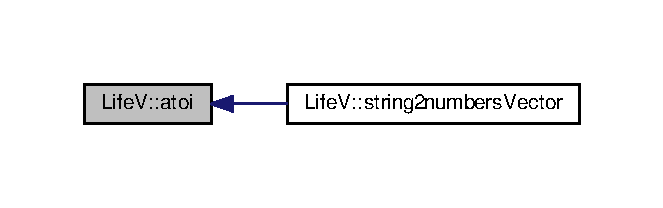
\includegraphics[width=318pt]{namespaceLifeV_a1a787279805886c5b208055992c29c9a_icgraph}
\end{center}
\end{figure}


\hypertarget{namespaceLifeV_aecf5099a32c6f096d09d0506ee79255b}{\index{Life\-V@{Life\-V}!eat\-Comments@{eat\-Comments}}
\index{eat\-Comments@{eat\-Comments}!LifeV@{Life\-V}}
\subsubsection[{eat\-Comments}]{\setlength{\rightskip}{0pt plus 5cm}std\-::istream \& Life\-V\-::eat\-Comments (
\begin{DoxyParamCaption}
\item[{std\-::istream \&}]{s}
\end{DoxyParamCaption}
)}}\label{namespaceLifeV_aecf5099a32c6f096d09d0506ee79255b}


skip lines starting with '!\%\#;\$' 


\begin{DoxyCode}
50 \{
51     \textcolor{keywordtype}{char} \hyperlink{lineare_8m_ae0323a9039add2978bf5b49550572c7c}{c} = \textcolor{charliteral}{'a'};
52     \hyperlink{god__e_8m_aaa7c61c7163e7fc36352afb33ce6c3dd}{s}.get( c ) ;
53     \textcolor{keywordflow}{while} ( c == \textcolor{charliteral}{'!'} ||
54             c == \textcolor{charliteral}{'%'} ||
55             c == \textcolor{charliteral}{'#'} ||
56             c == \textcolor{charliteral}{';'} ||
57             c == \textcolor{charliteral}{'$'} )
58     \{
59         \hyperlink{god__e_8m_aaa7c61c7163e7fc36352afb33ce6c3dd}{s} >> \hyperlink{namespaceLifeV_aa91d4c3fafd93fcbfb7d0aca2b771a02}{eatLine} ;
60         \hyperlink{god__e_8m_aaa7c61c7163e7fc36352afb33ce6c3dd}{s}.get( c ) ;
61     \}
62     \textcolor{keywordflow}{return} \hyperlink{god__e_8m_aaa7c61c7163e7fc36352afb33ce6c3dd}{s}.putback( c ) ;
63 \}\textcolor{comment}{// eatComments}
\end{DoxyCode}


Questo è il grafo delle chiamate per questa funzione\-:
\nopagebreak
\begin{figure}[H]
\begin{center}
\leavevmode
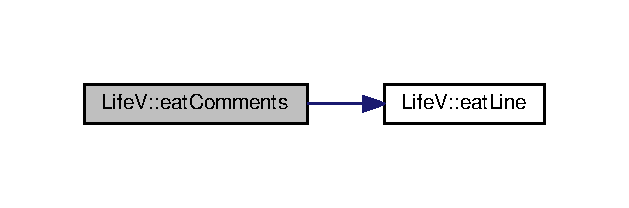
\includegraphics[width=302pt]{namespaceLifeV_aecf5099a32c6f096d09d0506ee79255b_cgraph}
\end{center}
\end{figure}




Questo è il grafo dei chiamanti di questa funzione\-:
\nopagebreak
\begin{figure}[H]
\begin{center}
\leavevmode
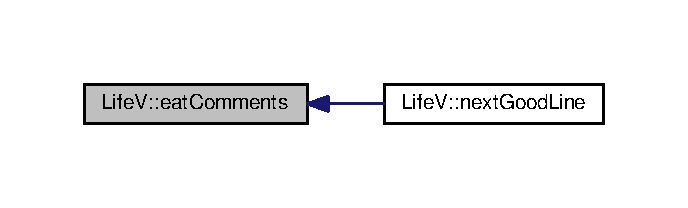
\includegraphics[width=330pt]{namespaceLifeV_aecf5099a32c6f096d09d0506ee79255b_icgraph}
\end{center}
\end{figure}


\hypertarget{namespaceLifeV_aa91d4c3fafd93fcbfb7d0aca2b771a02}{\index{Life\-V@{Life\-V}!eat\-Line@{eat\-Line}}
\index{eat\-Line@{eat\-Line}!LifeV@{Life\-V}}
\subsubsection[{eat\-Line}]{\setlength{\rightskip}{0pt plus 5cm}std\-::istream \& Life\-V\-::eat\-Line (
\begin{DoxyParamCaption}
\item[{std\-::istream \&}]{s}
\end{DoxyParamCaption}
)}}\label{namespaceLifeV_aa91d4c3fafd93fcbfb7d0aca2b771a02}
It gets a the next line from std\-::istream 
\begin{DoxyCode}
42 \{
43     \textcolor{keywordflow}{while} ( \hyperlink{god__e_8m_aaa7c61c7163e7fc36352afb33ce6c3dd}{s}.get() != \textcolor{charliteral}{'\(\backslash\)n'} && \hyperlink{god__e_8m_aaa7c61c7163e7fc36352afb33ce6c3dd}{s} . good() )
44         \{\}
45     \textcolor{keywordflow}{return} \hyperlink{god__e_8m_aaa7c61c7163e7fc36352afb33ce6c3dd}{s} ;
46 \}\textcolor{comment}{// eatLine}
\end{DoxyCode}


Questo è il grafo dei chiamanti di questa funzione\-:
\nopagebreak
\begin{figure}[H]
\begin{center}
\leavevmode
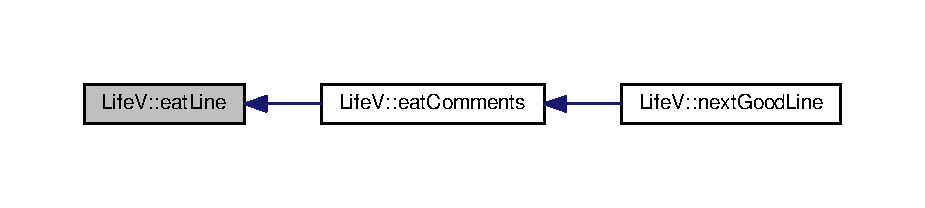
\includegraphics[width=350pt]{namespaceLifeV_aa91d4c3fafd93fcbfb7d0aca2b771a02_icgraph}
\end{center}
\end{figure}


\hypertarget{namespaceLifeV_a2e64a35012f78d9ab021477590e3bfaf}{\index{Life\-V@{Life\-V}!enum2\-String@{enum2\-String}}
\index{enum2\-String@{enum2\-String}!LifeV@{Life\-V}}
\subsubsection[{enum2\-String}]{\setlength{\rightskip}{0pt plus 5cm}template$<$typename Enumerator\-Type $>$ std\-::string Life\-V\-::enum2\-String (
\begin{DoxyParamCaption}
\item[{const Enumerator\-Type \&}]{Enum, }
\item[{const std\-::map$<$ std\-::string, Enumerator\-Type $>$ \&}]{Map}
\end{DoxyParamCaption}
)\hspace{0.3cm}{\ttfamily [inline]}}}\label{namespaceLifeV_a2e64a35012f78d9ab021477590e3bfaf}

\begin{DoxyCode}
147 \{
148     \textcolor{keywordflow}{for} ( \textcolor{keyword}{typename} std::map<std::string, EnumeratorType>::const\_iterator j = Map.begin();
149           j != Map.end() ; ++j )
150         \textcolor{keywordflow}{if} ( j->second == Enum )
151             \textcolor{keywordflow}{return} j->first;
152 
153     \textcolor{keywordflow}{return} \textcolor{stringliteral}{"NO\_TYPE\_FOUND"};
154 \}
\end{DoxyCode}
\hypertarget{namespaceLifeV_a2c4dd8a300964aa48909fce6ad5c72f5}{\index{Life\-V@{Life\-V}!next\-Good\-Line@{next\-Good\-Line}}
\index{next\-Good\-Line@{next\-Good\-Line}!LifeV@{Life\-V}}
\subsubsection[{next\-Good\-Line}]{\setlength{\rightskip}{0pt plus 5cm}std\-::istream \& Life\-V\-::next\-Good\-Line (
\begin{DoxyParamCaption}
\item[{std\-::istream \&}]{s, }
\item[{std\-::string \&}]{line}
\end{DoxyParamCaption}
)}}\label{namespaceLifeV_a2c4dd8a300964aa48909fce6ad5c72f5}


gets next uncommented line 


\begin{DoxyCode}
67 \{
68     \hyperlink{god__e_8m_aaa7c61c7163e7fc36352afb33ce6c3dd}{s} >> \hyperlink{namespaceLifeV_aecf5099a32c6f096d09d0506ee79255b}{eatComments};
69     getline( \hyperlink{god__e_8m_aaa7c61c7163e7fc36352afb33ce6c3dd}{s}, line );
70     \textcolor{keywordflow}{return} \hyperlink{god__e_8m_aaa7c61c7163e7fc36352afb33ce6c3dd}{s};
71 \}\textcolor{comment}{// nextGoodLine}
\end{DoxyCode}


Questo è il grafo delle chiamate per questa funzione\-:
\nopagebreak
\begin{figure}[H]
\begin{center}
\leavevmode
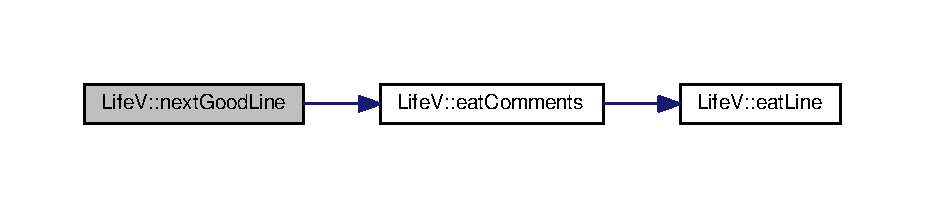
\includegraphics[width=350pt]{namespaceLifeV_a2c4dd8a300964aa48909fce6ad5c72f5_cgraph}
\end{center}
\end{figure}


\hypertarget{namespaceLifeV_a3c2a31cefb08654a69273a1a3bf11fac}{\index{Life\-V@{Life\-V}!number2string@{number2string}}
\index{number2string@{number2string}!LifeV@{Life\-V}}
\subsubsection[{number2string}]{\setlength{\rightskip}{0pt plus 5cm}template$<$typename Number\-Type $>$ std\-::string Life\-V\-::number2string (
\begin{DoxyParamCaption}
\item[{const Number\-Type \&}]{n}
\end{DoxyParamCaption}
)\hspace{0.3cm}{\ttfamily [inline]}}}\label{namespaceLifeV_a3c2a31cefb08654a69273a1a3bf11fac}

\begin{DoxyCode}
134 \{
135     std::stringstream out;
136     out << n;
137 
138     \textcolor{keywordflow}{return} out.str();
139 \}
\end{DoxyCode}
\hypertarget{namespaceLifeV_af57500c586141320ace55cf0b2a5c9fe}{\index{Life\-V@{Life\-V}!operator+@{operator+}}
\index{operator+@{operator+}!LifeV@{Life\-V}}
\subsubsection[{operator+}]{\setlength{\rightskip}{0pt plus 5cm}std\-::string Life\-V\-::operator+ (
\begin{DoxyParamCaption}
\item[{const std\-::string \&}]{str, }
\item[{const int}]{i}
\end{DoxyParamCaption}
)}}\label{namespaceLifeV_af57500c586141320ace55cf0b2a5c9fe}

\begin{DoxyCode}
99 \{
100     \textcolor{keywordtype}{int} digits = abs( \hyperlink{god__e_8m_a8604be5925f4266ab5ccc69675329c80}{i} ) / 10;
101     \textcolor{keywordtype}{char}* str\_i = \textcolor{keyword}{new} \textcolor{keywordtype}{char}[ digits ];
102     sprintf( str\_i, \textcolor{stringliteral}{"%i"}, \hyperlink{god__e_8m_a8604be5925f4266ab5ccc69675329c80}{i} );
103     std::string str2 = str + str\_i;
104     \textcolor{keyword}{delete}[] str\_i;
105     \textcolor{keywordflow}{return} str2;
106 \}\textcolor{comment}{// operator+}
\end{DoxyCode}
\hypertarget{namespaceLifeV_ae00b5ce86e0f837f3f3392074652b7ed}{\index{Life\-V@{Life\-V}!operator+@{operator+}}
\index{operator+@{operator+}!LifeV@{Life\-V}}
\subsubsection[{operator+}]{\setlength{\rightskip}{0pt plus 5cm}std\-::string Life\-V\-::operator+ (
\begin{DoxyParamCaption}
\item[{const std\-::string \&}]{str, }
\item[{const long int}]{i}
\end{DoxyParamCaption}
)}}\label{namespaceLifeV_ae00b5ce86e0f837f3f3392074652b7ed}
\hypertarget{namespaceLifeV_a54f5fa0ff0002920c744bcbaff350bc0}{\index{Life\-V@{Life\-V}!operator+@{operator+}}
\index{operator+@{operator+}!LifeV@{Life\-V}}
\subsubsection[{operator+}]{\setlength{\rightskip}{0pt plus 5cm}std\-::string Life\-V\-::operator+ (
\begin{DoxyParamCaption}
\item[{const std\-::string \&}]{str, }
\item[{const unsigned int}]{i}
\end{DoxyParamCaption}
)}}\label{namespaceLifeV_a54f5fa0ff0002920c744bcbaff350bc0}

\begin{DoxyCode}
120 \{
121     \textcolor{keywordtype}{int} digits = \hyperlink{god__e_8m_a8604be5925f4266ab5ccc69675329c80}{i} / 10;
122     \textcolor{keywordtype}{char}* str\_i = \textcolor{keyword}{new} \textcolor{keywordtype}{char}[ digits ];
123     sprintf( str\_i, \textcolor{stringliteral}{"%u"}, \hyperlink{god__e_8m_a8604be5925f4266ab5ccc69675329c80}{i} );
124     std::string str2 = str + str\_i;
125     \textcolor{keyword}{delete}[] str\_i;
126     \textcolor{keywordflow}{return} str2;
127 \}\textcolor{comment}{// operator+}
\end{DoxyCode}
\hypertarget{namespaceLifeV_aed80af702e5521c5fc90b0c33bbd5af3}{\index{Life\-V@{Life\-V}!operator+@{operator+}}
\index{operator+@{operator+}!LifeV@{Life\-V}}
\subsubsection[{operator+}]{\setlength{\rightskip}{0pt plus 5cm}std\-::string Life\-V\-::operator+ (
\begin{DoxyParamCaption}
\item[{const std\-::string \&}]{str, }
\item[{const long}]{i}
\end{DoxyParamCaption}
)}}\label{namespaceLifeV_aed80af702e5521c5fc90b0c33bbd5af3}

\begin{DoxyCode}
110 \{
111     \textcolor{keywordtype}{int} digits = abs( \hyperlink{god__e_8m_a8604be5925f4266ab5ccc69675329c80}{i} ) / 10;
112     \textcolor{keywordtype}{char}* str\_i = \textcolor{keyword}{new} \textcolor{keywordtype}{char}[ digits ];
113     sprintf( str\_i, \textcolor{stringliteral}{"%ld"}, \hyperlink{god__e_8m_a8604be5925f4266ab5ccc69675329c80}{i} );
114     std::string str2 = str + str\_i;
115     \textcolor{keyword}{delete}[] str\_i;
116     \textcolor{keywordflow}{return} str2;
117 \}\textcolor{comment}{// operator+}
\end{DoxyCode}
\hypertarget{namespaceLifeV_a200b22ebae8c113c2624f7195797d4a4}{\index{Life\-V@{Life\-V}!parse\-List@{parse\-List}}
\index{parse\-List@{parse\-List}!LifeV@{Life\-V}}
\subsubsection[{parse\-List}]{\setlength{\rightskip}{0pt plus 5cm}template$<$typename Entry\-Type $>$ void Life\-V\-::parse\-List (
\begin{DoxyParamCaption}
\item[{const std\-::string \&}]{slist, }
\item[{std\-::list$<$ Entry\-Type $>$ \&}]{list}
\end{DoxyParamCaption}
)}}\label{namespaceLifeV_a200b22ebae8c113c2624f7195797d4a4}

\begin{DoxyCode}
92 \{
93     std::string stringList = slist;
94     \textcolor{keywordflow}{if} ( slist == \textcolor{stringliteral}{""} )
95     \{
96         \textcolor{keywordflow}{return};
97     \}
98 
99     \textcolor{keywordtype}{int} commaPos = 0;
100 
101     \textcolor{keywordflow}{while} ( commaPos != (\textcolor{keywordtype}{int})std::string::npos )
102     \{
103         commaPos = stringList.find( \textcolor{stringliteral}{","} );
104 
105         std::stringstream stream;
106         stream <<  stringList.substr( 0, commaPos ).c\_str();
107 
108         EntryType var;
109         stream >> var;
110         list.push\_back( var );
111 
112         stringList = stringList.substr( commaPos + 1 );
113     \}
114 \}
\end{DoxyCode}
\hypertarget{namespaceLifeV_a5fb0107fd71b5be2c32f536619a73175}{\index{Life\-V@{Life\-V}!set\-String\-Length@{set\-String\-Length}}
\index{set\-String\-Length@{set\-String\-Length}!LifeV@{Life\-V}}
\subsubsection[{set\-String\-Length}]{\setlength{\rightskip}{0pt plus 5cm}std\-::string \& Life\-V\-::set\-String\-Length (
\begin{DoxyParamCaption}
\item[{std\-::string \&}]{s, }
\item[{unsigned int}]{len, }
\item[{char}]{c}
\end{DoxyParamCaption}
)}}\label{namespaceLifeV_a5fb0107fd71b5be2c32f536619a73175}
always return a std\-::string with len characters
\begin{DoxyItemize}
\item if the s has more than len characters \-: keep only the first len
\item if the s has less than len characters \-: complete with c until len 
\end{DoxyItemize}
\begin{DoxyCode}
75 \{
76     \textcolor{comment}{/*}
77 \textcolor{comment}{      always return a std::string with len characters}
78 \textcolor{comment}{        - if the s has more than len characters : keep only the first len}
79 \textcolor{comment}{        - if the s has less than len characters : complete with c until len}
80 \textcolor{comment}{    */}
81     std::string stmp( len, \hyperlink{lineare_8m_ae0323a9039add2978bf5b49550572c7c}{c} );
82     \textcolor{keywordflow}{if} ( \hyperlink{god__e_8m_aaa7c61c7163e7fc36352afb33ce6c3dd}{s}.length() > len )
83     \{
84         \hyperlink{god__e_8m_aaa7c61c7163e7fc36352afb33ce6c3dd}{s}.erase( len, \hyperlink{god__e_8m_aaa7c61c7163e7fc36352afb33ce6c3dd}{s}.length() );
85     \}
86     stmp.replace( 0, \hyperlink{god__e_8m_aaa7c61c7163e7fc36352afb33ce6c3dd}{s}.length(), \hyperlink{god__e_8m_aaa7c61c7163e7fc36352afb33ce6c3dd}{s} );
87     \hyperlink{god__e_8m_aaa7c61c7163e7fc36352afb33ce6c3dd}{s} = stmp;
88     \textcolor{keywordflow}{return} \hyperlink{god__e_8m_aaa7c61c7163e7fc36352afb33ce6c3dd}{s};
89 \}\textcolor{comment}{// setStringLength}
\end{DoxyCode}
\hypertarget{namespaceLifeV_a95341022bde9111ea53dfe204cbe70ae}{\index{Life\-V@{Life\-V}!string2number@{string2number}}
\index{string2number@{string2number}!LifeV@{Life\-V}}
\subsubsection[{string2number}]{\setlength{\rightskip}{0pt plus 5cm}double Life\-V\-::string2number (
\begin{DoxyParamCaption}
\item[{const std\-::string \&}]{s}
\end{DoxyParamCaption}
)\hspace{0.3cm}{\ttfamily [inline]}}}\label{namespaceLifeV_a95341022bde9111ea53dfe204cbe70ae}

\begin{DoxyCode}
120 \{
121     std::stringstream out;
122     out << \hyperlink{god__e_8m_aaa7c61c7163e7fc36352afb33ce6c3dd}{s};
123 
124     \textcolor{keywordtype}{double} n;
125     out >> n;
126 
127     \textcolor{keywordflow}{return} n;
128 \}
\end{DoxyCode}
\hypertarget{namespaceLifeV_a5f2c3319750ceebbeb2a3bb374a2596b}{\index{Life\-V@{Life\-V}!string2numbers\-Vector@{string2numbers\-Vector}}
\index{string2numbers\-Vector@{string2numbers\-Vector}!LifeV@{Life\-V}}
\subsubsection[{string2numbers\-Vector}]{\setlength{\rightskip}{0pt plus 5cm}template$<$typename Number\-Type $>$ void Life\-V\-::string2numbers\-Vector (
\begin{DoxyParamCaption}
\item[{const std\-::string \&}]{string, }
\item[{std\-::vector$<$ Number\-Type $>$ \&}]{number\-Vector}
\end{DoxyParamCaption}
)}}\label{namespaceLifeV_a5f2c3319750ceebbeb2a3bb374a2596b}

\begin{DoxyCode}
161 \{
162     \textcolor{comment}{//Split the string}
163     std::vector< std::string > stringVector;
164     boost::split( stringVector, \textcolor{keywordtype}{string}, boost::is\_any\_of( \textcolor{stringliteral}{","} ) );
165 
166     \textcolor{comment}{//Convert to the right type}
167     \textcolor{keywordflow}{for} ( \hyperlink{namespaceLifeV_a4bd093cf6b0d5b57b2d89e0e90d610b7}{UInt} \hyperlink{god__e_8m_a8604be5925f4266ab5ccc69675329c80}{i}( 0 ); i < static\_cast<UInt> ( stringVector.size() ); ++\hyperlink{god__e_8m_a8604be5925f4266ab5ccc69675329c80}{i} )
168         numberVector.push\_back( static\_cast<NumberType>( \hyperlink{namespaceLifeV_a1a787279805886c5b208055992c29c9a}{std::atoi}( stringVector[
      \hyperlink{god__e_8m_a8604be5925f4266ab5ccc69675329c80}{i}].c\_str())));
169 \}
\end{DoxyCode}


Questo è il grafo delle chiamate per questa funzione\-:
\nopagebreak
\begin{figure}[H]
\begin{center}
\leavevmode
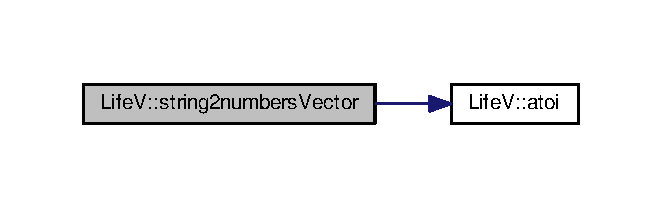
\includegraphics[width=318pt]{namespaceLifeV_a5f2c3319750ceebbeb2a3bb374a2596b_cgraph}
\end{center}
\end{figure}



\chapter{Documentazione delle classi}
\hypertarget{classBC}{\section{Riferimenti per la classe B\-C}
\label{classBC}\index{B\-C@{B\-C}}
}


{\ttfamily \#include $<$B\-C.\-h$>$}

\subsection*{Membri pubblici}
\begin{DoxyCompactItemize}
\item 
\hyperlink{classBC_a67ec843bf00c68c63aa5f701d0c0119b}{B\-C} (const Get\-Pot \&data\-File, const std\-::string \&section, getfem\-::mesh \&mesh, const std\-::string \&Mesh\-Type, const std\-::string \&section\-Saturation=\char`\"{}saturation/\char`\"{})
\end{DoxyCompactItemize}


\subsection{Documentazione dei costruttori e dei distruttori}
\hypertarget{classBC_a67ec843bf00c68c63aa5f701d0c0119b}{\index{B\-C@{B\-C}!B\-C@{B\-C}}
\index{B\-C@{B\-C}!BC@{B\-C}}
\subsubsection[{B\-C}]{\setlength{\rightskip}{0pt plus 5cm}B\-C\-::\-B\-C (
\begin{DoxyParamCaption}
\item[{const Get\-Pot \&}]{data\-File, }
\item[{const std\-::string \&}]{section, }
\item[{getfem\-::mesh \&}]{mesh, }
\item[{const std\-::string \&}]{Mesh\-Type, }
\item[{const std\-::string \&}]{section\-Saturation = {\ttfamily \char`\"{}saturation/\char`\"{}}}
\end{DoxyParamCaption}
)}}\label{classBC_a67ec843bf00c68c63aa5f701d0c0119b}

\begin{DoxyCode}
14                                              :
15          M\_meshFEM(mesh),
16          M\_section ( section ),
17          M\_sectionSaturation ( M\_section + sectionSaturation )
18 \{\};
\end{DoxyCode}


La documentazione per questa classe è stata generata a partire dai seguenti file\-:\begin{DoxyCompactItemize}
\item 
include/\hyperlink{BC_8h}{B\-C.\-h}\item 
src/\hyperlink{BC_8cc}{B\-C.\-cc}\end{DoxyCompactItemize}

\hypertarget{classBCHandler}{\section{Riferimenti per la classe B\-C\-Handler}
\label{classBCHandler}\index{B\-C\-Handler@{B\-C\-Handler}}
}


{\ttfamily \#include $<$B\-C\-Handler.\-h$>$}

\subsection*{Membri pubblici}
\begin{DoxyCompactItemize}
\item 
\hyperlink{classBCHandler_af15c3846a782d6b7db1985c69929c388}{B\-C\-Handler} (const \hyperlink{BC_8h_ae127263052e0676d0fe233f834ca7227}{B\-C\-Ptr\-Container\-\_\-\-Type} \&fracture\-B\-C)
\item 
const \hyperlink{BC_8h_a088c36f945ad8f6e7e0c7c423994c6ec}{B\-C\-Ptr\-\_\-\-Type} \& \hyperlink{classBCHandler_a2ab65711f8ee3643ecf19de52ceab470}{get\-Fracture\-B\-C} (const size\-\_\-type \&id) const 
\end{DoxyCompactItemize}


\subsection{Documentazione dei costruttori e dei distruttori}
\hypertarget{classBCHandler_af15c3846a782d6b7db1985c69929c388}{\index{B\-C\-Handler@{B\-C\-Handler}!B\-C\-Handler@{B\-C\-Handler}}
\index{B\-C\-Handler@{B\-C\-Handler}!BCHandler@{B\-C\-Handler}}
\subsubsection[{B\-C\-Handler}]{\setlength{\rightskip}{0pt plus 5cm}B\-C\-Handler\-::\-B\-C\-Handler (
\begin{DoxyParamCaption}
\item[{const {\bf B\-C\-Ptr\-Container\-\_\-\-Type} \&}]{fracture\-B\-C}
\end{DoxyParamCaption}
)}}\label{classBCHandler_af15c3846a782d6b7db1985c69929c388}

\begin{DoxyCode}
9                                                              :
10                        M\_fractureBC(fractureBC)
11 \{
12 \}
\end{DoxyCode}


\subsection{Documentazione delle funzioni membro}
\hypertarget{classBCHandler_a2ab65711f8ee3643ecf19de52ceab470}{\index{B\-C\-Handler@{B\-C\-Handler}!get\-Fracture\-B\-C@{get\-Fracture\-B\-C}}
\index{get\-Fracture\-B\-C@{get\-Fracture\-B\-C}!BCHandler@{B\-C\-Handler}}
\subsubsection[{get\-Fracture\-B\-C}]{\setlength{\rightskip}{0pt plus 5cm}const {\bf B\-C\-Ptr\-\_\-\-Type}\& B\-C\-Handler\-::get\-Fracture\-B\-C (
\begin{DoxyParamCaption}
\item[{const size\-\_\-type \&}]{id}
\end{DoxyParamCaption}
) const\hspace{0.3cm}{\ttfamily [inline]}}}\label{classBCHandler_a2ab65711f8ee3643ecf19de52ceab470}

\begin{DoxyCode}
35     \{
36         \textcolor{keywordflow}{return} M\_fractureBC [ id ];
37     \}
\end{DoxyCode}


La documentazione per questa classe è stata generata a partire dai seguenti file\-:\begin{DoxyCompactItemize}
\item 
include/\hyperlink{BCHandler_8h}{B\-C\-Handler.\-h}\item 
src/\hyperlink{BCHandler_8cc}{B\-C\-Handler.\-cc}\end{DoxyCompactItemize}

\hypertarget{classExporter}{\section{Riferimenti per la classe Exporter}
\label{classExporter}\index{Exporter@{Exporter}}
}


{\ttfamily \#include $<$Exporter.\-h$>$}

\subsection*{Membri pubblici}
\begin{DoxyCompactItemize}
\item 
\hyperlink{classExporter_a14a838ecbf8b9f5a370013430236081f}{Exporter} (const Get\-Pot \&data\-File, const std\-::string \&section=\char`\"{}\char`\"{})
\begin{DoxyCompactList}\small\item\em Costruttore che fissa la cartella dove esportare i risultati. \end{DoxyCompactList}\item 
const std\-::string \& \hyperlink{classExporter_a2771781a7f08fe8518973a6ba712a391}{get\-Folder} () const 
\item 
void \hyperlink{classExporter_a8ca0bdf8550569260ef4f3e39ab274dc}{spy} (const \hyperlink{Core_8h_a87137a9501b38c724ac80bc955164bb7}{sparse\-Matrix\-Ptr\-\_\-\-Type} \&matrix, const std\-::string \&name\-File) const 
\begin{DoxyCompactList}\small\item\em Funzione che esporta una matrice di tipo sparso. \end{DoxyCompactList}\item 
void \hyperlink{classExporter_ab5452c31e85ecfbbda8623aa20723e68}{spy} (const \hyperlink{Core_8h_ab09b6fa3c23db1b8c60456f8690c44a7}{scalar\-Vector\-Ptr\-\_\-\-Type} \&vector, const std\-::string \&name\-File) const 
\begin{DoxyCompactList}\small\item\em Funzione che esporta un vettore di scalari. \end{DoxyCompactList}\item 
void \hyperlink{classExporter_af02a2344019769ab23d9ac673a7b3709}{mesh\-Region} (const getfem\-::mesh \&mesh, const std\-::string \&name\-File=\char`\"{}Region\-Mesh.\-vtk\char`\"{}) const 
\begin{DoxyCompactList}\small\item\em Funzione che esporta le regioni della mesh. \end{DoxyCompactList}\end{DoxyCompactItemize}


\subsection{Documentazione dei costruttori e dei distruttori}
\hypertarget{classExporter_a14a838ecbf8b9f5a370013430236081f}{\index{Exporter@{Exporter}!Exporter@{Exporter}}
\index{Exporter@{Exporter}!Exporter@{Exporter}}
\subsubsection[{Exporter}]{\setlength{\rightskip}{0pt plus 5cm}Exporter\-::\-Exporter (
\begin{DoxyParamCaption}
\item[{const Get\-Pot \&}]{data\-File, }
\item[{const std\-::string \&}]{section = {\ttfamily \char`\"{}\char`\"{}}}
\end{DoxyParamCaption}
)}}\label{classExporter_a14a838ecbf8b9f5a370013430236081f}


Costruttore che fissa la cartella dove esportare i risultati. 


\begin{DoxyParams}{Parametri}
{\em data\-File} & variabile di tipo Get\-Pot che contiene il nome del file data \\
\hline
{\em section} & stringa con il nome della sezione in cui leggere \\
\hline
\end{DoxyParams}

\begin{DoxyCode}
9                                                                       :
10                     M\_vtkFolder(dataFile((section + \textcolor{stringliteral}{"folderVTK"}).data(), \textcolor{stringliteral}{"./vtk/"}))
11 \{
12 \}\textcolor{comment}{// costruttore}
\end{DoxyCode}


\subsection{Documentazione delle funzioni membro}
\hypertarget{classExporter_a2771781a7f08fe8518973a6ba712a391}{\index{Exporter@{Exporter}!get\-Folder@{get\-Folder}}
\index{get\-Folder@{get\-Folder}!Exporter@{Exporter}}
\subsubsection[{get\-Folder}]{\setlength{\rightskip}{0pt plus 5cm}const std\-::string\& Exporter\-::get\-Folder (
\begin{DoxyParamCaption}
{}
\end{DoxyParamCaption}
) const\hspace{0.3cm}{\ttfamily [inline]}}}\label{classExporter_a2771781a7f08fe8518973a6ba712a391}
\begin{DoxyReturn}{Restituisce}
std\-::string\& M\-\_\-vtk\-Folder\-: stringa col nome della cartella di esportazione 
\end{DoxyReturn}

\begin{DoxyCode}
43     \{
44         \textcolor{keywordflow}{return} M\_vtkFolder;
45     \}
\end{DoxyCode}
\hypertarget{classExporter_af02a2344019769ab23d9ac673a7b3709}{\index{Exporter@{Exporter}!mesh\-Region@{mesh\-Region}}
\index{mesh\-Region@{mesh\-Region}!Exporter@{Exporter}}
\subsubsection[{mesh\-Region}]{\setlength{\rightskip}{0pt plus 5cm}void Exporter\-::mesh\-Region (
\begin{DoxyParamCaption}
\item[{const getfem\-::mesh \&}]{mesh, }
\item[{const std\-::string \&}]{name\-File = {\ttfamily \char`\"{}RegionMesh.vtk\char`\"{}}}
\end{DoxyParamCaption}
) const}}\label{classExporter_af02a2344019769ab23d9ac673a7b3709}


Funzione che esporta le regioni della mesh. 


\begin{DoxyParams}{Parametri}
{\em getfem\-::mesh\&} & mesh\-: mesh di supporto \\
\hline
{\em std\-::string\&} & name\-File = \char`\"{}\-Region\-Mesh.\-vtk\char`\"{}\-: nome del file su cui scrivere la soluzione, se non è dato è posto di default pari a \char`\"{}\-Region\-Mesh.\-vtk\char`\"{} \\
\hline
\end{DoxyParams}
\hypertarget{classExporter_a8ca0bdf8550569260ef4f3e39ab274dc}{\index{Exporter@{Exporter}!spy@{spy}}
\index{spy@{spy}!Exporter@{Exporter}}
\subsubsection[{spy}]{\setlength{\rightskip}{0pt plus 5cm}void Exporter\-::spy (
\begin{DoxyParamCaption}
\item[{const {\bf sparse\-Matrix\-Ptr\-\_\-\-Type} \&}]{matrix, }
\item[{const std\-::string \&}]{name\-File}
\end{DoxyParamCaption}
) const}}\label{classExporter_a8ca0bdf8550569260ef4f3e39ab274dc}


Funzione che esporta una matrice di tipo sparso. 


\begin{DoxyParams}{Parametri}
{\em sparse\-Matrix\-Ptr\-\_\-\-Type\&} & matrix\-: matrice sparsa \\
\hline
{\em td\-::string\&} & name\-File\-: nome del file in cui esportare \\
\hline
\end{DoxyParams}

\begin{DoxyCode}
16 \{
17     gmm::MatrixMarket\_IO::write(nameFile.c\_str(), *matrix);
18 
19     \textcolor{keywordflow}{return};
20 
21 \} \textcolor{comment}{// spy}
\end{DoxyCode}
\hypertarget{classExporter_ab5452c31e85ecfbbda8623aa20723e68}{\index{Exporter@{Exporter}!spy@{spy}}
\index{spy@{spy}!Exporter@{Exporter}}
\subsubsection[{spy}]{\setlength{\rightskip}{0pt plus 5cm}void Exporter\-::spy (
\begin{DoxyParamCaption}
\item[{const {\bf scalar\-Vector\-Ptr\-\_\-\-Type} \&}]{vector, }
\item[{const std\-::string \&}]{name\-File}
\end{DoxyParamCaption}
) const}}\label{classExporter_ab5452c31e85ecfbbda8623aa20723e68}


Funzione che esporta un vettore di scalari. 


\begin{DoxyParams}{Parametri}
{\em scalar\-Vector\-Ptr\-\_\-\-Type\&} & vector\-: vettore di scalari \\
\hline
{\em std\-::string\&} & name\-File\-: nome del file in cui esportare \\
\hline
\end{DoxyParams}

\begin{DoxyCode}
25 \{
26     std::ofstream file;
27     file.open(nameFile.c\_str());
28     \textcolor{keywordflow}{for} ( size\_type \hyperlink{god__e_8m_a8604be5925f4266ab5ccc69675329c80}{i} = 0; \hyperlink{god__e_8m_a8604be5925f4266ab5ccc69675329c80}{i} < vector->size(); ++\hyperlink{god__e_8m_a8604be5925f4266ab5ccc69675329c80}{i} )
29     \{
30         file << std::setprecision(15) << vector->at(\hyperlink{god__e_8m_a8604be5925f4266ab5ccc69675329c80}{i}) << std::endl;
31     \}
32     file.close();
33 
34     \textcolor{keywordflow}{return};
35 
36 \} \textcolor{comment}{// spy}
\end{DoxyCode}


La documentazione per questa classe è stata generata a partire dai seguenti file\-:\begin{DoxyCompactItemize}
\item 
include/\hyperlink{Exporter_8h}{Exporter.\-h}\item 
src/\hyperlink{Exporter_8cc}{Exporter.\-cc}\end{DoxyCompactItemize}

\hypertarget{classFluxHandler}{\section{Riferimenti per la classe Flux\-Handler}
\label{classFluxHandler}\index{Flux\-Handler@{Flux\-Handler}}
}


{\ttfamily \#include $<$Flux\-Handler.\-h$>$}

\subsection*{Membri pubblici}
\begin{DoxyCompactItemize}
\item 
\hyperlink{classFluxHandler_a2dfd526283bcbbd9b085086483da6f1f}{Flux\-Handler} (const Get\-Pot \&data\-File, const std\-::string \&section\-Flux)
\item 
std\-::string \hyperlink{classFluxHandler_a14ae8f3fdcb387025bacbad018e87f21}{get\-Flux} () const 
\item 
std\-::string \hyperlink{classFluxHandler_a5bbc2d196b5ff3d10e0b48b7024bbf85}{get\-Flux1} () const 
\item 
scalar\-\_\-type \hyperlink{classFluxHandler_a30989bb4704c83aa4ac88e6630eadb68}{get\-Us} () const 
\end{DoxyCompactItemize}


\subsection{Documentazione dei costruttori e dei distruttori}
\hypertarget{classFluxHandler_a2dfd526283bcbbd9b085086483da6f1f}{\index{Flux\-Handler@{Flux\-Handler}!Flux\-Handler@{Flux\-Handler}}
\index{Flux\-Handler@{Flux\-Handler}!FluxHandler@{Flux\-Handler}}
\subsubsection[{Flux\-Handler}]{\setlength{\rightskip}{0pt plus 5cm}Flux\-Handler\-::\-Flux\-Handler (
\begin{DoxyParamCaption}
\item[{const Get\-Pot \&}]{data\-File, }
\item[{const std\-::string \&}]{section\-Flux}
\end{DoxyParamCaption}
)}}\label{classFluxHandler_a2dfd526283bcbbd9b085086483da6f1f}

\begin{DoxyCode}
10                                                                                :
11                          M\_sectionFlux ( sectionFlux ),
12                          M\_flux ( dataFile ( ( M\_sectionFlux + \textcolor{stringliteral}{"f"} ).data (), \textcolor{stringliteral}{"x*x./2"} ) ),
13                          M\_flux1 ( dataFile ( ( M\_sectionFlux + \textcolor{stringliteral}{"f1"} ).data (), \textcolor{stringliteral}{"x"} ) ),
14                          M\_Us ( dataFile ( ( M\_sectionFlux + \textcolor{stringliteral}{"us"} ).data (), 0.5 ) )
15 \{\}
\end{DoxyCode}


\subsection{Documentazione delle funzioni membro}
\hypertarget{classFluxHandler_a14ae8f3fdcb387025bacbad018e87f21}{\index{Flux\-Handler@{Flux\-Handler}!get\-Flux@{get\-Flux}}
\index{get\-Flux@{get\-Flux}!FluxHandler@{Flux\-Handler}}
\subsubsection[{get\-Flux}]{\setlength{\rightskip}{0pt plus 5cm}std\-::string Flux\-Handler\-::get\-Flux (
\begin{DoxyParamCaption}
{}
\end{DoxyParamCaption}
) const\hspace{0.3cm}{\ttfamily [inline]}}}\label{classFluxHandler_a14ae8f3fdcb387025bacbad018e87f21}

\begin{DoxyCode}
34     \{
35         \textcolor{keywordflow}{return} M\_flux;
36     \}
\end{DoxyCode}
\hypertarget{classFluxHandler_a5bbc2d196b5ff3d10e0b48b7024bbf85}{\index{Flux\-Handler@{Flux\-Handler}!get\-Flux1@{get\-Flux1}}
\index{get\-Flux1@{get\-Flux1}!FluxHandler@{Flux\-Handler}}
\subsubsection[{get\-Flux1}]{\setlength{\rightskip}{0pt plus 5cm}std\-::string Flux\-Handler\-::get\-Flux1 (
\begin{DoxyParamCaption}
{}
\end{DoxyParamCaption}
) const\hspace{0.3cm}{\ttfamily [inline]}}}\label{classFluxHandler_a5bbc2d196b5ff3d10e0b48b7024bbf85}

\begin{DoxyCode}
39     \{
40         \textcolor{keywordflow}{return} M\_flux1;
41     \}
\end{DoxyCode}
\hypertarget{classFluxHandler_a30989bb4704c83aa4ac88e6630eadb68}{\index{Flux\-Handler@{Flux\-Handler}!get\-Us@{get\-Us}}
\index{get\-Us@{get\-Us}!FluxHandler@{Flux\-Handler}}
\subsubsection[{get\-Us}]{\setlength{\rightskip}{0pt plus 5cm}scalar\-\_\-type Flux\-Handler\-::get\-Us (
\begin{DoxyParamCaption}
{}
\end{DoxyParamCaption}
) const\hspace{0.3cm}{\ttfamily [inline]}}}\label{classFluxHandler_a30989bb4704c83aa4ac88e6630eadb68}

\begin{DoxyCode}
44     \{
45         \textcolor{keywordflow}{return} M\_Us;
46     \}
\end{DoxyCode}


La documentazione per questa classe è stata generata a partire dai seguenti file\-:\begin{DoxyCompactItemize}
\item 
include/\hyperlink{FluxHandler_8h}{Flux\-Handler.\-h}\item 
src/\hyperlink{FluxHandler_8cc}{Flux\-Handler.\-cc}\end{DoxyCompactItemize}

\hypertarget{classFractureData}{\section{Riferimenti per la classe Fracture\-Data}
\label{classFractureData}\index{Fracture\-Data@{Fracture\-Data}}
}


{\ttfamily \#include $<$Fracture\-Data.\-h$>$}

\subsection*{Membri pubblici}
\begin{DoxyCompactItemize}
\item 
\hyperlink{classFractureData_a321da1e480bfd583c6a2c561ba1e0cf8}{Fracture\-Data} (const Get\-Pot \&data\-File, const std\-::string \&section=\char`\"{}fracture\-Data/\char`\"{}, const std\-::string \&section\-Domain=\char`\"{}domain/\char`\"{}, const std\-::string \&section\-Saturation=\char`\"{}saturation/\char`\"{})
\item 
void \hyperlink{classFractureData_a49671c83ba3f6501803913c224177a72}{feval} (\hyperlink{Core_8h_a4e75b5863535ba1dd79942de2846eff0}{scalar\-Vector\-\_\-\-Type} \&fl, const \hyperlink{Core_8h_a4e75b5863535ba1dd79942de2846eff0}{scalar\-Vector\-\_\-\-Type} \&\hyperlink{init_8m_aada26031cbb47e8d74da9873f5c1e3e1}{u0}, const size\-\_\-type \hyperlink{god__e_8m_a8604be5925f4266ab5ccc69675329c80}{i}, const size\-\_\-type \hyperlink{god__e_8m_a8ea372f7ee3c01d11fc4b4d13b8e6a75}{f})
\item 
scalar\-\_\-type \hyperlink{classFractureData_a8f6e19cc2575dd30498eb144d1d17554}{feval\-\_\-scal} (const scalar\-\_\-type \&us, const size\-\_\-type \hyperlink{god__e_8m_a8ea372f7ee3c01d11fc4b4d13b8e6a75}{f}=0)
\item 
scalar\-\_\-type \hyperlink{classFractureData_ae9fcfaedfb880fe7ef5bfe9eaffe0e50}{fzero} (const std\-::string \&\hyperlink{god__e_8m_a8ea372f7ee3c01d11fc4b4d13b8e6a75}{f}, const scalar\-\_\-type \&\hyperlink{init_8m_ab6991d210d93a78cdbdf6de1889c1259}{a}, const scalar\-\_\-type \&\hyperlink{rieman_8m_a21ad0bd836b90d08f4cf640b4c298e7c}{b}, size\-\_\-type count=0)
\item 
std\-::string \hyperlink{classFractureData_abc0da4d74175c7530375ad9368efb5f1}{get\-Flux} (const size\-\_\-type \&\hyperlink{god__e_8m_a8604be5925f4266ab5ccc69675329c80}{i})
\item 
std\-::string \hyperlink{classFractureData_aa30d8efee63dc3173cdd9864c9549ccf}{get\-Flux1} (const size\-\_\-type \&\hyperlink{god__e_8m_a8604be5925f4266ab5ccc69675329c80}{i})
\item 
scalar\-\_\-type \hyperlink{classFractureData_ab79d66dd830b6e1c55ade0d940c5c8cf}{mesh\-Spacing} (const scalar\-\_\-type \&\hyperlink{risultati__bastian_8m_a9336ebf25087d91c818ee6e9ec29f8c1}{x})
\item 
scalar\-\_\-type \hyperlink{classFractureData_a9598cf66a822a593e819df754420a2c2}{velocity} (const scalar\-\_\-type \&\hyperlink{god__e_8m_a5d13973cebbcfb3c9181cd74c7bc1812}{u})
\item 
scalar\-\_\-type \hyperlink{classFractureData_aab77ec8a8d3e878b5dfb72deb48841e7}{porosity} (const scalar\-\_\-type \&\hyperlink{god__e_8m_a5d13973cebbcfb3c9181cd74c7bc1812}{u})
\item 
scalar\-\_\-type \hyperlink{classFractureData_a142a1bb428365b60ed002362ca566517}{get\-Ci} (const scalar\-\_\-type \&\hyperlink{risultati__bastian_8m_a9336ebf25087d91c818ee6e9ec29f8c1}{x})
\item 
scalar\-\_\-type \hyperlink{classFractureData_a3ecc0d132f9cc105af6b24d676a7b9c5}{get\-Thickness} () const 
\item 
scalar\-\_\-type \hyperlink{classFractureData_abaebcf16d83713858e25837939ad3161}{get\-Length\-Abscissa} () const 
\item 
scalar\-\_\-type \hyperlink{classFractureData_a905e953f685b1329ddcc7ee56f8302b1}{get\-Length\-Ordinate} () const 
\item 
scalar\-\_\-type \hyperlink{classFractureData_a79747fff53da9d858950d83ad0114288}{get\-Length\-Quota} () const 
\item 
scalar\-\_\-type \hyperlink{classFractureData_aea2090efbba4e6aaa89e90864a1d46f6}{get\-A} () const 
\item 
scalar\-\_\-type \hyperlink{classFractureData_ad8a5510e522711cc9f2430a0b9fadc70}{get\-B} () const 
\item 
scalar\-\_\-type \hyperlink{classFractureData_a7ef5fdbdc462f4135d44102d2017c63b}{get\-H} () const 
\item 
scalar\-\_\-type \hyperlink{classFractureData_aeb3c6a78af1e2746bf5ce69c9ae8945d}{get\-Spatial\-Discretization} () const 
\item 
scalar\-\_\-type \hyperlink{classFractureData_a4b310767d1a91b0cef404093aacfab82}{get\-Space\-Dimension} () const 
\item 
std\-::string \hyperlink{classFractureData_aaded6c0452470489beb4ab95b5f4158f}{get\-Mesh\-Type} () const 
\item 
std\-::string \hyperlink{classFractureData_a2df7c1f0a0722878d4ccdca537605dac}{get\-Bc} () const 
\item 
size\-\_\-type \hyperlink{classFractureData_ab6b8416e26e0b37b9789d83336d37fef}{get\-Number\-Flux} () const 
\item 
scalar\-\_\-type \hyperlink{classFractureData_a875649432017de65d85176395e42376c}{get\-Xd} () const 
\item 
scalar\-\_\-type \hyperlink{classFractureData_a2695260e58e519fc0fa1c79a475d776d}{get\-Cfl} ()
\end{DoxyCompactItemize}


\subsection{Documentazione dei costruttori e dei distruttori}
\hypertarget{classFractureData_a321da1e480bfd583c6a2c561ba1e0cf8}{\index{Fracture\-Data@{Fracture\-Data}!Fracture\-Data@{Fracture\-Data}}
\index{Fracture\-Data@{Fracture\-Data}!FractureData@{Fracture\-Data}}
\subsubsection[{Fracture\-Data}]{\setlength{\rightskip}{0pt plus 5cm}Fracture\-Data\-::\-Fracture\-Data (
\begin{DoxyParamCaption}
\item[{const Get\-Pot \&}]{data\-File, }
\item[{const std\-::string \&}]{section = {\ttfamily \char`\"{}fractureData/\char`\"{}}, }
\item[{const std\-::string \&}]{section\-Domain = {\ttfamily \char`\"{}domain/\char`\"{}}, }
\item[{const std\-::string \&}]{section\-Saturation = {\ttfamily \char`\"{}saturation/\char`\"{}}}
\end{DoxyParamCaption}
)}}\label{classFractureData_a321da1e480bfd583c6a2c561ba1e0cf8}

\begin{DoxyCode}
12                                                                  :
13                              M\_section ( section ),
14                              M\_sectionDomain ( M\_section + sectionDomain ),
15                              M\_sectionSaturation ( M\_section + sectionSaturation ),
16                              \textcolor{comment}{// domain}
17                              M\_thickness ( dataFile ( ( M\_sectionDomain + \textcolor{stringliteral}{"thickness"} ).data (), 0.01 ) ),
18                              M\_lengthAbscissa ( dataFile ( ( M\_sectionDomain + \textcolor{stringliteral}{"lengthAbscissa"} ).data (), 
      1. ) ),
19                              M\_lengthOrdinate ( dataFile ( ( M\_sectionDomain + \textcolor{stringliteral}{"lengthOrdinate"} ).data (), 
      0. ) ),
20                              M\_lengthQuota ( dataFile ( ( M\_sectionDomain + \textcolor{stringliteral}{"lengthQuota"} ).data (), 0. ) )
      ,
21                              M\_a ( dataFile ( ( M\_sectionDomain + \textcolor{stringliteral}{"a"} ).data (), -1. ) ),
22                              M\_b ( dataFile ( ( M\_sectionDomain + \textcolor{stringliteral}{"b"} ).data (), 1. ) ),
23                              M\_spatialDiscretization ( dataFile ( ( M\_sectionDomain + \textcolor{stringliteral}{"
      spatialDiscretization"} ).data (), 200 ) ),
24                              M\_translateAbscissa ( dataFile ( ( M\_sectionDomain + \textcolor{stringliteral}{"translateAbscissa"} ).
      data (), 0. ) ),
25                              M\_spaceDimension ( dataFile ( ( M\_section + \textcolor{stringliteral}{"spaceDimension"} ).data (), 1. ) )
      ,
26                              M\_meshType ( dataFile ( ( M\_sectionDomain + \textcolor{stringliteral}{"meshType"} ).data (), \textcolor{stringliteral}{"GT\_PK(1,1)"}
       ) ),
27                              M\_meshSpacing( dataFile ( ( M\_sectionDomain + \textcolor{stringliteral}{"spacing"} ).data (), \textcolor{stringliteral}{"x"} ) ),
28                              \textcolor{comment}{// saturation}
29                              M\_bc ( dataFile ( ( M\_sectionSaturation + \textcolor{stringliteral}{"bc"}).data (), \textcolor{stringliteral}{"p"} ) ),
30                              M\_u0 ( dataFile ( ( M\_sectionSaturation + \textcolor{stringliteral}{"u0"}).data (), \textcolor{stringliteral}{"1."} ) ),
31                              M\_numberFlux( dataFile ( ( M\_sectionSaturation + \textcolor{stringliteral}{"numberFlux"}).data (), 1 ) ),
32                              M\_x( dataFile ( ( M\_sectionSaturation + \textcolor{stringliteral}{"x0"}).data (), 0. ) ),
33                              M\_cfl ( dataFile ( ( M\_sectionSaturation + \textcolor{stringliteral}{"cfl"} ).data (), 1.8 ) ),
34                              M\_U ( dataFile ( (M\_sectionSaturation + \textcolor{stringliteral}{"U"} ).data (), \textcolor{stringliteral}{"1."} ) ),
35                              M\_invP ( dataFile ( (M\_sectionSaturation + \textcolor{stringliteral}{"invPorosity"} ).data (), \textcolor{stringliteral}{"1."} ) )
36 \{
37     M\_h = ( M\_b-M\_a )/(M\_spatialDiscretization-2);
38 
39     M\_flux.resize( M\_numberFlux );
40 
41     std::ostringstream sectionFlux;
42 
43     \textcolor{keywordflow}{for} ( size\_type \hyperlink{god__e_8m_a8604be5925f4266ab5ccc69675329c80}{i} = 0; \hyperlink{god__e_8m_a8604be5925f4266ab5ccc69675329c80}{i} < M\_numberFlux; \hyperlink{god__e_8m_a8604be5925f4266ab5ccc69675329c80}{i}++ )
44     \{
45         sectionFlux << M\_sectionSaturation << \textcolor{stringliteral}{"fluxData"} << \hyperlink{god__e_8m_a8604be5925f4266ab5ccc69675329c80}{i} << \textcolor{stringliteral}{"/"};
46 
47         M\_flux [ \hyperlink{god__e_8m_a8604be5925f4266ab5ccc69675329c80}{i} ].reset( \textcolor{keyword}{new} \hyperlink{FluxHandler_8h_aead2274079d41aa00d7e649c4377b875}{FluxHandler\_Type}( dataFile, sectionFlux.str() ));
48 
49     \}
50 
51 \}\textcolor{comment}{// costruttore}
\end{DoxyCode}


\subsection{Documentazione delle funzioni membro}
\hypertarget{classFractureData_a49671c83ba3f6501803913c224177a72}{\index{Fracture\-Data@{Fracture\-Data}!feval@{feval}}
\index{feval@{feval}!FractureData@{Fracture\-Data}}
\subsubsection[{feval}]{\setlength{\rightskip}{0pt plus 5cm}void Fracture\-Data\-::feval (
\begin{DoxyParamCaption}
\item[{{\bf scalar\-Vector\-\_\-\-Type} \&}]{fl, }
\item[{const {\bf scalar\-Vector\-\_\-\-Type} \&}]{u0, }
\item[{const size\-\_\-type}]{i, }
\item[{const size\-\_\-type}]{f}
\end{DoxyParamCaption}
)}}\label{classFractureData_a49671c83ba3f6501803913c224177a72}

\begin{DoxyCode}
55 \{
56     \hyperlink{confronto_8m_a96d7a28b6a4428be15fc1017d19343fa}{flux}.clear();
57 
58     std::string Flux;
59 
60     \textcolor{keywordflow}{for} ( size\_type j = 0; j < \hyperlink{god__e_8m_ae060ce5868d35ef17bcb6e832da03be9}{u0}.size(); j++ )
61     \{
62         scalar\_type U = \hyperlink{classFractureData_a9598cf66a822a593e819df754420a2c2}{velocity} ( \hyperlink{god__e_8m_ae060ce5868d35ef17bcb6e832da03be9}{u0} [ j ]);
63         scalar\_type P = \hyperlink{classFractureData_aab77ec8a8d3e878b5dfb72deb48841e7}{porosity} ( \hyperlink{god__e_8m_ae060ce5868d35ef17bcb6e832da03be9}{u0} [ j ]);
64 
65         \textcolor{keywordflow}{if}( \hyperlink{god__e_8m_a8604be5925f4266ab5ccc69675329c80}{i} == 1)
66         \{
67             Flux = M\_flux [ \hyperlink{god__e_8m_a68f477f9b30a6300d5af9b02eac82f35}{f} ]->getFlux();
68         \}
69         \textcolor{keywordflow}{else}
70         \{
71             Flux = M\_flux [ \hyperlink{god__e_8m_a68f477f9b30a6300d5af9b02eac82f35}{f} ]->getFlux1();
72         \}
73         M\_parser.\hyperlink{classLifeV_1_1Parser_ac05769e836a0dc95d9c020df361a5194}{setString} ( Flux );
74         M\_parser.\hyperlink{classLifeV_1_1Parser_aa2b362e12b8feb60231705d499c9fbae}{setVariable} ( \textcolor{stringliteral}{"x"}, \hyperlink{god__e_8m_ae060ce5868d35ef17bcb6e832da03be9}{u0} [ j ] );
75 
76         \hyperlink{confronto_8m_a96d7a28b6a4428be15fc1017d19343fa}{flux}.push\_back( U*P*M\_parser.\hyperlink{classLifeV_1_1Parser_a51d84fd4ae6d420620e7beee58fad673}{evaluate} () );
77 
78     \}
79     \textcolor{keywordflow}{return};
80 \}\textcolor{comment}{// feval}
\end{DoxyCode}


Questo è il grafo delle chiamate per questa funzione\-:
\nopagebreak
\begin{figure}[H]
\begin{center}
\leavevmode
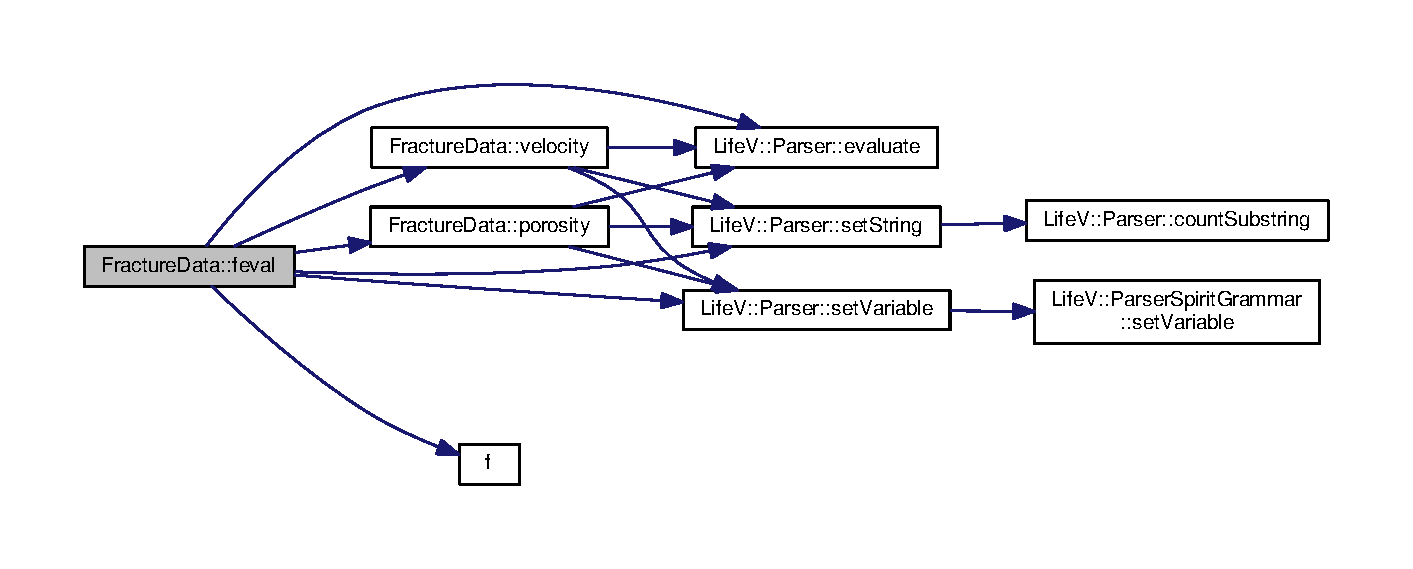
\includegraphics[width=350pt]{classFractureData_a49671c83ba3f6501803913c224177a72_cgraph}
\end{center}
\end{figure}


\hypertarget{classFractureData_a8f6e19cc2575dd30498eb144d1d17554}{\index{Fracture\-Data@{Fracture\-Data}!feval\-\_\-scal@{feval\-\_\-scal}}
\index{feval\-\_\-scal@{feval\-\_\-scal}!FractureData@{Fracture\-Data}}
\subsubsection[{feval\-\_\-scal}]{\setlength{\rightskip}{0pt plus 5cm}scalar\-\_\-type Fracture\-Data\-::feval\-\_\-scal (
\begin{DoxyParamCaption}
\item[{const scalar\-\_\-type \&}]{us, }
\item[{const size\-\_\-type}]{f = {\ttfamily 0}}
\end{DoxyParamCaption}
)}}\label{classFractureData_a8f6e19cc2575dd30498eb144d1d17554}

\begin{DoxyCode}
85 \{
86     scalar\_type U = \hyperlink{classFractureData_a9598cf66a822a593e819df754420a2c2}{velocity} ( us );
87     scalar\_type P = \hyperlink{classFractureData_aab77ec8a8d3e878b5dfb72deb48841e7}{porosity} ( us );
88 
89     std::string Flux;
90 
91     \textcolor{keywordflow}{if} ( \hyperlink{god__e_8m_a68f477f9b30a6300d5af9b02eac82f35}{f} == 0 )
92     \{
93         Flux = M\_flux [ 0 ]->getFlux();
94 
95         M\_parser.\hyperlink{classLifeV_1_1Parser_ac05769e836a0dc95d9c020df361a5194}{setString} ( Flux );
96 
97         M\_parser.\hyperlink{classLifeV_1_1Parser_aa2b362e12b8feb60231705d499c9fbae}{setVariable} ( \textcolor{stringliteral}{"x"}, us );
98 
99         \textcolor{keywordflow}{return} U*P*M\_parser.\hyperlink{classLifeV_1_1Parser_a51d84fd4ae6d420620e7beee58fad673}{evaluate} ();
100     \}
101     \textcolor{keywordflow}{else}
102     \{
103         Flux = M\_flux [ 0 ]->getFlux1();
104 
105         M\_parser.\hyperlink{classLifeV_1_1Parser_ac05769e836a0dc95d9c020df361a5194}{setString} ( Flux );
106 
107         M\_parser.\hyperlink{classLifeV_1_1Parser_aa2b362e12b8feb60231705d499c9fbae}{setVariable} ( \textcolor{stringliteral}{"x"}, us );
108 
109         \textcolor{keywordflow}{return} U*P*M\_parser.\hyperlink{classLifeV_1_1Parser_a51d84fd4ae6d420620e7beee58fad673}{evaluate} ();
110 
111     \}
112 
113 \}\textcolor{comment}{// feval\_scal}
\end{DoxyCode}


Questo è il grafo delle chiamate per questa funzione\-:
\nopagebreak
\begin{figure}[H]
\begin{center}
\leavevmode
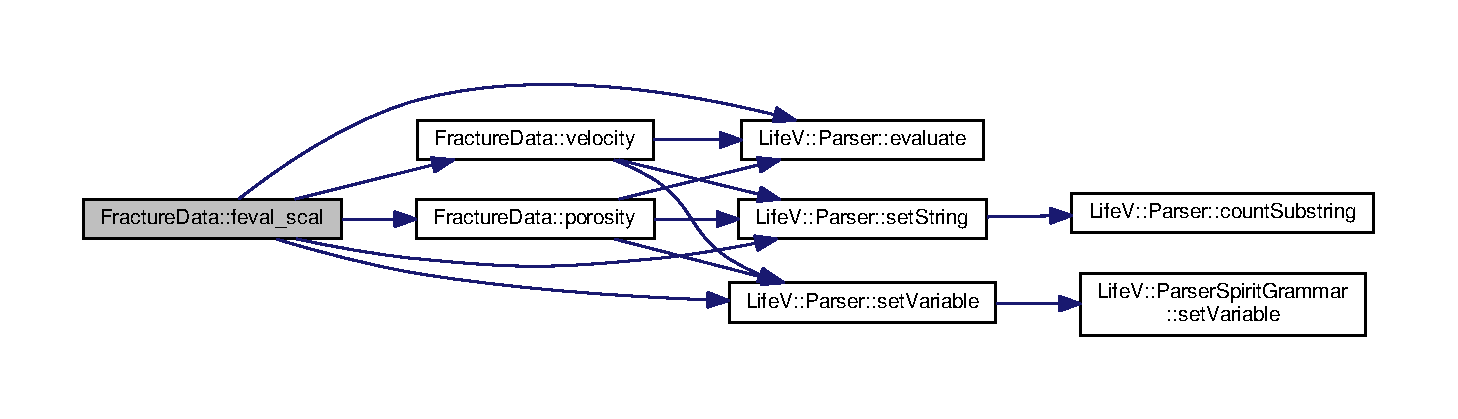
\includegraphics[width=350pt]{classFractureData_a8f6e19cc2575dd30498eb144d1d17554_cgraph}
\end{center}
\end{figure}


\hypertarget{classFractureData_ae9fcfaedfb880fe7ef5bfe9eaffe0e50}{\index{Fracture\-Data@{Fracture\-Data}!fzero@{fzero}}
\index{fzero@{fzero}!FractureData@{Fracture\-Data}}
\subsubsection[{fzero}]{\setlength{\rightskip}{0pt plus 5cm}scalar\-\_\-type Fracture\-Data\-::fzero (
\begin{DoxyParamCaption}
\item[{const std\-::string \&}]{f, }
\item[{const scalar\-\_\-type \&}]{a, }
\item[{const scalar\-\_\-type \&}]{b, }
\item[{size\-\_\-type}]{count = {\ttfamily 0}}
\end{DoxyParamCaption}
)}}\label{classFractureData_ae9fcfaedfb880fe7ef5bfe9eaffe0e50}

\begin{DoxyCode}
117 \{
118     scalar\_type toll = 1.0E-7;
119     size\_type itermax = 100;
120     scalar\_type x0;
121 
122     M\_parser.\hyperlink{classLifeV_1_1Parser_ac05769e836a0dc95d9c020df361a5194}{setString} ( \hyperlink{god__e_8m_a68f477f9b30a6300d5af9b02eac82f35}{f} );
123 
124     M\_parser.\hyperlink{classLifeV_1_1Parser_aa2b362e12b8feb60231705d499c9fbae}{setVariable} ( \textcolor{stringliteral}{"x"}, \hyperlink{init_8m_ab6991d210d93a78cdbdf6de1889c1259}{a} );
125 
126     scalar\_type f\_a = M\_parser.\hyperlink{classLifeV_1_1Parser_a51d84fd4ae6d420620e7beee58fad673}{evaluate} ();
127 
128     \textcolor{keywordflow}{if} ( f\_a < toll )
129     \{
130         \textcolor{keywordflow}{return} \hyperlink{init_8m_ab6991d210d93a78cdbdf6de1889c1259}{a};
131     \}
132     M\_parser.\hyperlink{classLifeV_1_1Parser_aa2b362e12b8feb60231705d499c9fbae}{setVariable} ( \textcolor{stringliteral}{"x"}, \hyperlink{init_8m_a21ad0bd836b90d08f4cf640b4c298e7c}{b} );
133 
134     scalar\_type f\_b = M\_parser.\hyperlink{classLifeV_1_1Parser_a51d84fd4ae6d420620e7beee58fad673}{evaluate} ();
135 
136     \textcolor{keywordflow}{if} ( f\_b < toll )
137     \{
138         \textcolor{keywordflow}{return} \hyperlink{init_8m_a21ad0bd836b90d08f4cf640b4c298e7c}{b};
139     \}
140 
141     scalar\_type \hyperlink{lineare_8m_ae0323a9039add2978bf5b49550572c7c}{c} = ( \hyperlink{init_8m_ab6991d210d93a78cdbdf6de1889c1259}{a} + \hyperlink{init_8m_a21ad0bd836b90d08f4cf640b4c298e7c}{b} )/2;
142 
143     M\_parser.\hyperlink{classLifeV_1_1Parser_aa2b362e12b8feb60231705d499c9fbae}{setVariable} ( \textcolor{stringliteral}{"x"}, c );
144 
145     scalar\_type f\_c = M\_parser.\hyperlink{classLifeV_1_1Parser_a51d84fd4ae6d420620e7beee58fad673}{evaluate} ();
146 
147 
148     \textcolor{keywordflow}{if} ( f\_c < toll )
149     \{
150         \textcolor{keywordflow}{return} \hyperlink{lineare_8m_ae0323a9039add2978bf5b49550572c7c}{c};
151     \}
152 
153     \textcolor{keywordflow}{if} ( count < itermax )
154     \{
155         \textcolor{keywordflow}{if} ( f\_a * f\_c <0 )
156         \{
157             x0 = \hyperlink{classFractureData_ae9fcfaedfb880fe7ef5bfe9eaffe0e50}{fzero}( \hyperlink{god__e_8m_a68f477f9b30a6300d5af9b02eac82f35}{f}, \hyperlink{init_8m_ab6991d210d93a78cdbdf6de1889c1259}{a}, c, count+1 );
158         \}
159         \textcolor{keywordflow}{else}
160         \{
161             x0 = \hyperlink{classFractureData_ae9fcfaedfb880fe7ef5bfe9eaffe0e50}{fzero}( \hyperlink{god__e_8m_a68f477f9b30a6300d5af9b02eac82f35}{f}, c, \hyperlink{init_8m_a21ad0bd836b90d08f4cf640b4c298e7c}{b}, count+1 );
162         \}
163     \}
164     \textcolor{keywordflow}{else}
165     \{
166         \textcolor{keywordflow}{return} x0;
167     \}
168 
169     \textcolor{keywordflow}{return} x0;
170 \}\textcolor{comment}{// fzero}
\end{DoxyCode}


Questo è il grafo delle chiamate per questa funzione\-:
\nopagebreak
\begin{figure}[H]
\begin{center}
\leavevmode
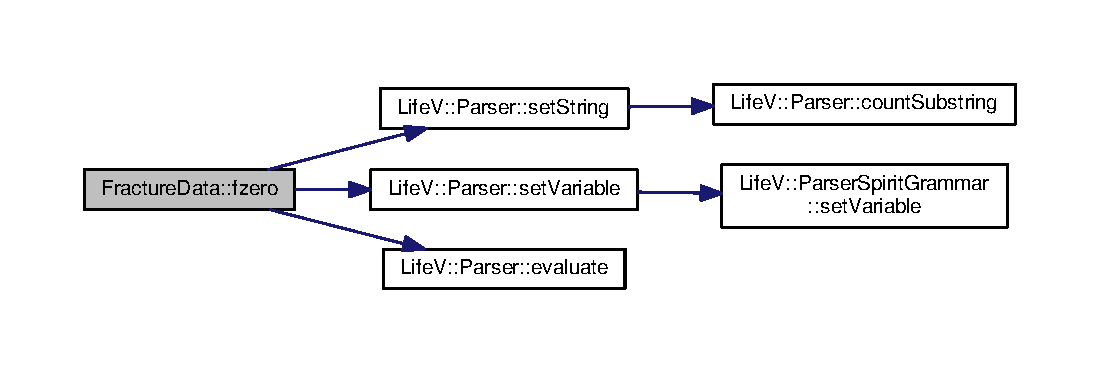
\includegraphics[width=350pt]{classFractureData_ae9fcfaedfb880fe7ef5bfe9eaffe0e50_cgraph}
\end{center}
\end{figure}


\hypertarget{classFractureData_aea2090efbba4e6aaa89e90864a1d46f6}{\index{Fracture\-Data@{Fracture\-Data}!get\-A@{get\-A}}
\index{get\-A@{get\-A}!FractureData@{Fracture\-Data}}
\subsubsection[{get\-A}]{\setlength{\rightskip}{0pt plus 5cm}scalar\-\_\-type Fracture\-Data\-::get\-A (
\begin{DoxyParamCaption}
{}
\end{DoxyParamCaption}
) const\hspace{0.3cm}{\ttfamily [inline]}}}\label{classFractureData_aea2090efbba4e6aaa89e90864a1d46f6}

\begin{DoxyCode}
72     \{
73         \textcolor{keywordflow}{return} M\_a;
74     \}
\end{DoxyCode}
\hypertarget{classFractureData_ad8a5510e522711cc9f2430a0b9fadc70}{\index{Fracture\-Data@{Fracture\-Data}!get\-B@{get\-B}}
\index{get\-B@{get\-B}!FractureData@{Fracture\-Data}}
\subsubsection[{get\-B}]{\setlength{\rightskip}{0pt plus 5cm}scalar\-\_\-type Fracture\-Data\-::get\-B (
\begin{DoxyParamCaption}
{}
\end{DoxyParamCaption}
) const\hspace{0.3cm}{\ttfamily [inline]}}}\label{classFractureData_ad8a5510e522711cc9f2430a0b9fadc70}

\begin{DoxyCode}
77     \{
78         \textcolor{keywordflow}{return} M\_b;
79     \}
\end{DoxyCode}
\hypertarget{classFractureData_a2df7c1f0a0722878d4ccdca537605dac}{\index{Fracture\-Data@{Fracture\-Data}!get\-Bc@{get\-Bc}}
\index{get\-Bc@{get\-Bc}!FractureData@{Fracture\-Data}}
\subsubsection[{get\-Bc}]{\setlength{\rightskip}{0pt plus 5cm}std\-::string Fracture\-Data\-::get\-Bc (
\begin{DoxyParamCaption}
{}
\end{DoxyParamCaption}
) const\hspace{0.3cm}{\ttfamily [inline]}}}\label{classFractureData_a2df7c1f0a0722878d4ccdca537605dac}

\begin{DoxyCode}
102     \{
103         \textcolor{keywordflow}{return} M\_bc;
104     \}
\end{DoxyCode}
\hypertarget{classFractureData_a2695260e58e519fc0fa1c79a475d776d}{\index{Fracture\-Data@{Fracture\-Data}!get\-Cfl@{get\-Cfl}}
\index{get\-Cfl@{get\-Cfl}!FractureData@{Fracture\-Data}}
\subsubsection[{get\-Cfl}]{\setlength{\rightskip}{0pt plus 5cm}scalar\-\_\-type Fracture\-Data\-::get\-Cfl (
\begin{DoxyParamCaption}
{}
\end{DoxyParamCaption}
)\hspace{0.3cm}{\ttfamily [inline]}}}\label{classFractureData_a2695260e58e519fc0fa1c79a475d776d}

\begin{DoxyCode}
117     \{
118         \textcolor{keywordflow}{return} M\_cfl;
119     \}
\end{DoxyCode}
\hypertarget{classFractureData_a142a1bb428365b60ed002362ca566517}{\index{Fracture\-Data@{Fracture\-Data}!get\-Ci@{get\-Ci}}
\index{get\-Ci@{get\-Ci}!FractureData@{Fracture\-Data}}
\subsubsection[{get\-Ci}]{\setlength{\rightskip}{0pt plus 5cm}scalar\-\_\-type Fracture\-Data\-::get\-Ci (
\begin{DoxyParamCaption}
\item[{const scalar\-\_\-type \&}]{x}
\end{DoxyParamCaption}
)}}\label{classFractureData_a142a1bb428365b60ed002362ca566517}

\begin{DoxyCode}
213 \{
214 
215     M\_parser.\hyperlink{classLifeV_1_1Parser_ac05769e836a0dc95d9c020df361a5194}{setString}( M\_u0 );
216     M\_parser.\hyperlink{classLifeV_1_1Parser_aa2b362e12b8feb60231705d499c9fbae}{setVariable} ( \textcolor{stringliteral}{"x"}, \hyperlink{confronto_8m_ad2e52d4a42a755ccd73c8de47175afa3}{x} );
217 
218     \textcolor{keywordflow}{return} M\_parser.\hyperlink{classLifeV_1_1Parser_a51d84fd4ae6d420620e7beee58fad673}{evaluate} ();
219 
220     \textcolor{comment}{/*}
221 \textcolor{comment}{    if( x == -4.0 )}
222 \textcolor{comment}{    \{}
223 \textcolor{comment}{        return 1.;}
224 \textcolor{comment}{    \}}
225 \textcolor{comment}{    else}
226 \textcolor{comment}{    \{}
227 \textcolor{comment}{        return 0;}
228 \textcolor{comment}{    \}}
229 \textcolor{comment}{    */}
230 \}\textcolor{comment}{// getCi}
\end{DoxyCode}


Questo è il grafo delle chiamate per questa funzione\-:
\nopagebreak
\begin{figure}[H]
\begin{center}
\leavevmode
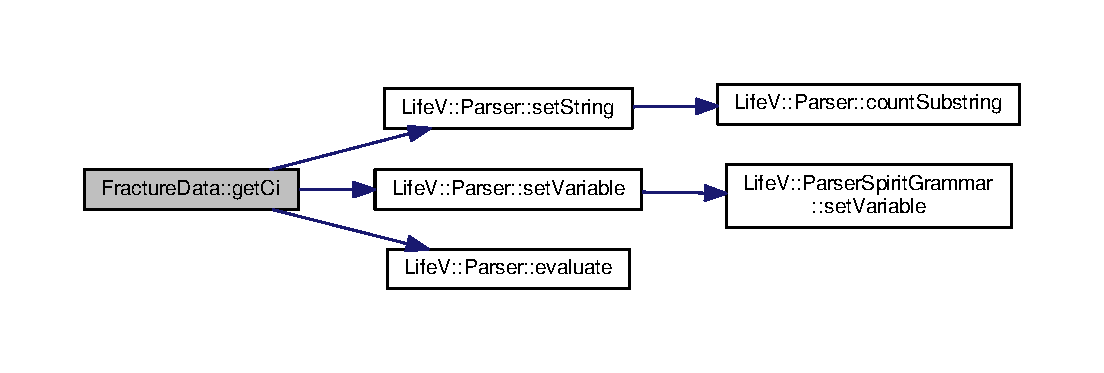
\includegraphics[width=350pt]{classFractureData_a142a1bb428365b60ed002362ca566517_cgraph}
\end{center}
\end{figure}




Questo è il grafo dei chiamanti di questa funzione\-:
\nopagebreak
\begin{figure}[H]
\begin{center}
\leavevmode
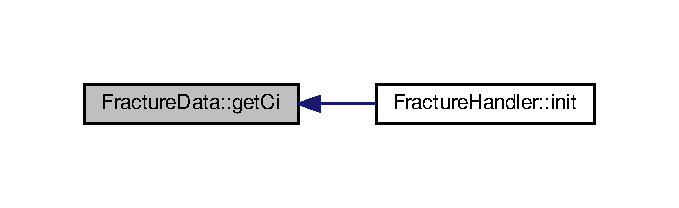
\includegraphics[width=326pt]{classFractureData_a142a1bb428365b60ed002362ca566517_icgraph}
\end{center}
\end{figure}


\hypertarget{classFractureData_abc0da4d74175c7530375ad9368efb5f1}{\index{Fracture\-Data@{Fracture\-Data}!get\-Flux@{get\-Flux}}
\index{get\-Flux@{get\-Flux}!FractureData@{Fracture\-Data}}
\subsubsection[{get\-Flux}]{\setlength{\rightskip}{0pt plus 5cm}std\-::string Fracture\-Data\-::get\-Flux (
\begin{DoxyParamCaption}
\item[{const size\-\_\-type \&}]{i}
\end{DoxyParamCaption}
)}}\label{classFractureData_abc0da4d74175c7530375ad9368efb5f1}

\begin{DoxyCode}
174 \{
175     \textcolor{keywordflow}{return} M\_flux [ \hyperlink{god__e_8m_a8604be5925f4266ab5ccc69675329c80}{i} ]->getFlux();
176 \}\textcolor{comment}{// getFlux}
\end{DoxyCode}
\hypertarget{classFractureData_aa30d8efee63dc3173cdd9864c9549ccf}{\index{Fracture\-Data@{Fracture\-Data}!get\-Flux1@{get\-Flux1}}
\index{get\-Flux1@{get\-Flux1}!FractureData@{Fracture\-Data}}
\subsubsection[{get\-Flux1}]{\setlength{\rightskip}{0pt plus 5cm}std\-::string Fracture\-Data\-::get\-Flux1 (
\begin{DoxyParamCaption}
\item[{const size\-\_\-type \&}]{i}
\end{DoxyParamCaption}
)}}\label{classFractureData_aa30d8efee63dc3173cdd9864c9549ccf}

\begin{DoxyCode}
180 \{
181     \textcolor{keywordflow}{return} M\_flux [ \hyperlink{god__e_8m_a8604be5925f4266ab5ccc69675329c80}{i} ]->getFlux1();
182 \}\textcolor{comment}{// getFlux1}
\end{DoxyCode}
\hypertarget{classFractureData_a7ef5fdbdc462f4135d44102d2017c63b}{\index{Fracture\-Data@{Fracture\-Data}!get\-H@{get\-H}}
\index{get\-H@{get\-H}!FractureData@{Fracture\-Data}}
\subsubsection[{get\-H}]{\setlength{\rightskip}{0pt plus 5cm}scalar\-\_\-type Fracture\-Data\-::get\-H (
\begin{DoxyParamCaption}
{}
\end{DoxyParamCaption}
) const\hspace{0.3cm}{\ttfamily [inline]}}}\label{classFractureData_a7ef5fdbdc462f4135d44102d2017c63b}

\begin{DoxyCode}
82     \{
83         \textcolor{keywordflow}{return} M\_h;
84     \}
\end{DoxyCode}
\hypertarget{classFractureData_abaebcf16d83713858e25837939ad3161}{\index{Fracture\-Data@{Fracture\-Data}!get\-Length\-Abscissa@{get\-Length\-Abscissa}}
\index{get\-Length\-Abscissa@{get\-Length\-Abscissa}!FractureData@{Fracture\-Data}}
\subsubsection[{get\-Length\-Abscissa}]{\setlength{\rightskip}{0pt plus 5cm}scalar\-\_\-type Fracture\-Data\-::get\-Length\-Abscissa (
\begin{DoxyParamCaption}
{}
\end{DoxyParamCaption}
) const\hspace{0.3cm}{\ttfamily [inline]}}}\label{classFractureData_abaebcf16d83713858e25837939ad3161}

\begin{DoxyCode}
57     \{
58         \textcolor{keywordflow}{return} M\_lengthAbscissa;
59     \}
\end{DoxyCode}


Questo è il grafo dei chiamanti di questa funzione\-:
\nopagebreak
\begin{figure}[H]
\begin{center}
\leavevmode
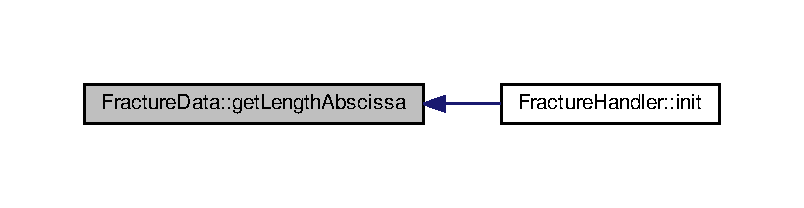
\includegraphics[width=350pt]{classFractureData_abaebcf16d83713858e25837939ad3161_icgraph}
\end{center}
\end{figure}


\hypertarget{classFractureData_a905e953f685b1329ddcc7ee56f8302b1}{\index{Fracture\-Data@{Fracture\-Data}!get\-Length\-Ordinate@{get\-Length\-Ordinate}}
\index{get\-Length\-Ordinate@{get\-Length\-Ordinate}!FractureData@{Fracture\-Data}}
\subsubsection[{get\-Length\-Ordinate}]{\setlength{\rightskip}{0pt plus 5cm}scalar\-\_\-type Fracture\-Data\-::get\-Length\-Ordinate (
\begin{DoxyParamCaption}
{}
\end{DoxyParamCaption}
) const\hspace{0.3cm}{\ttfamily [inline]}}}\label{classFractureData_a905e953f685b1329ddcc7ee56f8302b1}

\begin{DoxyCode}
62     \{
63         \textcolor{keywordflow}{return} M\_lengthOrdinate;
64     \}
\end{DoxyCode}


Questo è il grafo dei chiamanti di questa funzione\-:
\nopagebreak
\begin{figure}[H]
\begin{center}
\leavevmode
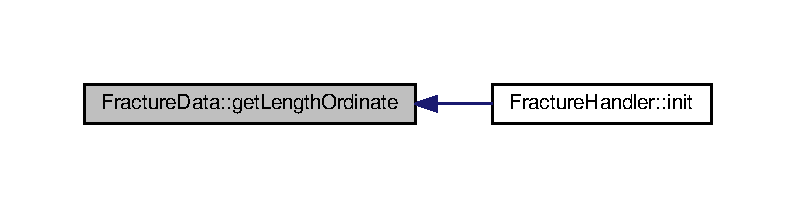
\includegraphics[width=350pt]{classFractureData_a905e953f685b1329ddcc7ee56f8302b1_icgraph}
\end{center}
\end{figure}


\hypertarget{classFractureData_a79747fff53da9d858950d83ad0114288}{\index{Fracture\-Data@{Fracture\-Data}!get\-Length\-Quota@{get\-Length\-Quota}}
\index{get\-Length\-Quota@{get\-Length\-Quota}!FractureData@{Fracture\-Data}}
\subsubsection[{get\-Length\-Quota}]{\setlength{\rightskip}{0pt plus 5cm}scalar\-\_\-type Fracture\-Data\-::get\-Length\-Quota (
\begin{DoxyParamCaption}
{}
\end{DoxyParamCaption}
) const\hspace{0.3cm}{\ttfamily [inline]}}}\label{classFractureData_a79747fff53da9d858950d83ad0114288}

\begin{DoxyCode}
67     \{
68         \textcolor{keywordflow}{return} M\_lengthQuota;
69     \}
\end{DoxyCode}


Questo è il grafo dei chiamanti di questa funzione\-:
\nopagebreak
\begin{figure}[H]
\begin{center}
\leavevmode
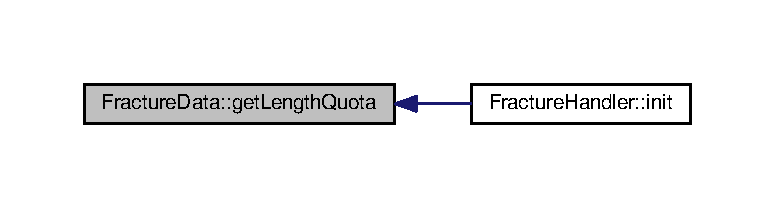
\includegraphics[width=350pt]{classFractureData_a79747fff53da9d858950d83ad0114288_icgraph}
\end{center}
\end{figure}


\hypertarget{classFractureData_aaded6c0452470489beb4ab95b5f4158f}{\index{Fracture\-Data@{Fracture\-Data}!get\-Mesh\-Type@{get\-Mesh\-Type}}
\index{get\-Mesh\-Type@{get\-Mesh\-Type}!FractureData@{Fracture\-Data}}
\subsubsection[{get\-Mesh\-Type}]{\setlength{\rightskip}{0pt plus 5cm}std\-::string Fracture\-Data\-::get\-Mesh\-Type (
\begin{DoxyParamCaption}
{}
\end{DoxyParamCaption}
) const\hspace{0.3cm}{\ttfamily [inline]}}}\label{classFractureData_aaded6c0452470489beb4ab95b5f4158f}

\begin{DoxyCode}
97     \{
98         \textcolor{keywordflow}{return} M\_meshType;
99     \}
\end{DoxyCode}


Questo è il grafo dei chiamanti di questa funzione\-:
\nopagebreak
\begin{figure}[H]
\begin{center}
\leavevmode
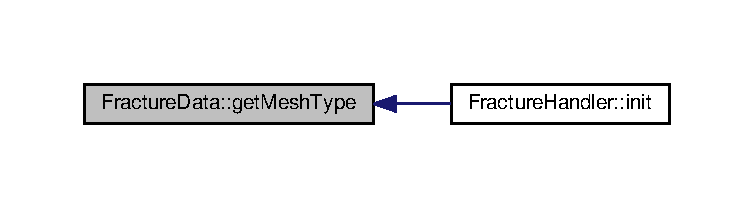
\includegraphics[width=350pt]{classFractureData_aaded6c0452470489beb4ab95b5f4158f_icgraph}
\end{center}
\end{figure}


\hypertarget{classFractureData_ab6b8416e26e0b37b9789d83336d37fef}{\index{Fracture\-Data@{Fracture\-Data}!get\-Number\-Flux@{get\-Number\-Flux}}
\index{get\-Number\-Flux@{get\-Number\-Flux}!FractureData@{Fracture\-Data}}
\subsubsection[{get\-Number\-Flux}]{\setlength{\rightskip}{0pt plus 5cm}size\-\_\-type Fracture\-Data\-::get\-Number\-Flux (
\begin{DoxyParamCaption}
{}
\end{DoxyParamCaption}
) const\hspace{0.3cm}{\ttfamily [inline]}}}\label{classFractureData_ab6b8416e26e0b37b9789d83336d37fef}

\begin{DoxyCode}
107     \{
108         \textcolor{keywordflow}{return} M\_numberFlux;
109     \}
\end{DoxyCode}
\hypertarget{classFractureData_a4b310767d1a91b0cef404093aacfab82}{\index{Fracture\-Data@{Fracture\-Data}!get\-Space\-Dimension@{get\-Space\-Dimension}}
\index{get\-Space\-Dimension@{get\-Space\-Dimension}!FractureData@{Fracture\-Data}}
\subsubsection[{get\-Space\-Dimension}]{\setlength{\rightskip}{0pt plus 5cm}scalar\-\_\-type Fracture\-Data\-::get\-Space\-Dimension (
\begin{DoxyParamCaption}
{}
\end{DoxyParamCaption}
) const\hspace{0.3cm}{\ttfamily [inline]}}}\label{classFractureData_a4b310767d1a91b0cef404093aacfab82}

\begin{DoxyCode}
92     \{
93         \textcolor{keywordflow}{return} M\_spaceDimension;
94     \}
\end{DoxyCode}


Questo è il grafo dei chiamanti di questa funzione\-:
\nopagebreak
\begin{figure}[H]
\begin{center}
\leavevmode
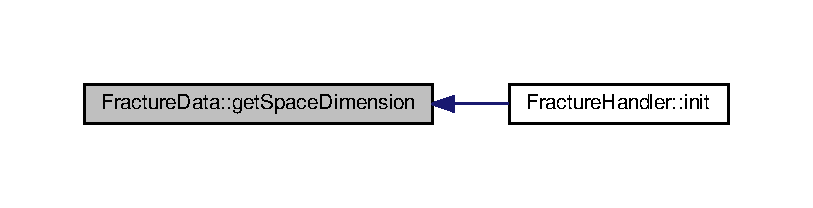
\includegraphics[width=350pt]{classFractureData_a4b310767d1a91b0cef404093aacfab82_icgraph}
\end{center}
\end{figure}


\hypertarget{classFractureData_aeb3c6a78af1e2746bf5ce69c9ae8945d}{\index{Fracture\-Data@{Fracture\-Data}!get\-Spatial\-Discretization@{get\-Spatial\-Discretization}}
\index{get\-Spatial\-Discretization@{get\-Spatial\-Discretization}!FractureData@{Fracture\-Data}}
\subsubsection[{get\-Spatial\-Discretization}]{\setlength{\rightskip}{0pt plus 5cm}scalar\-\_\-type Fracture\-Data\-::get\-Spatial\-Discretization (
\begin{DoxyParamCaption}
{}
\end{DoxyParamCaption}
) const\hspace{0.3cm}{\ttfamily [inline]}}}\label{classFractureData_aeb3c6a78af1e2746bf5ce69c9ae8945d}

\begin{DoxyCode}
87     \{
88         \textcolor{keywordflow}{return} M\_spatialDiscretization;
89     \}
\end{DoxyCode}


Questo è il grafo dei chiamanti di questa funzione\-:
\nopagebreak
\begin{figure}[H]
\begin{center}
\leavevmode
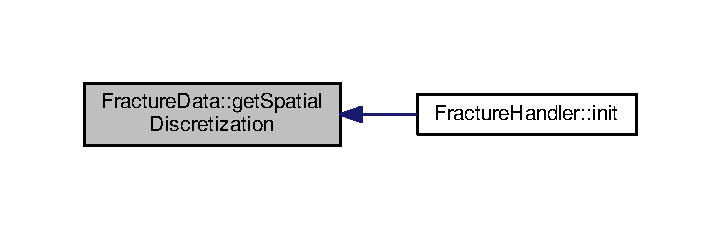
\includegraphics[width=346pt]{classFractureData_aeb3c6a78af1e2746bf5ce69c9ae8945d_icgraph}
\end{center}
\end{figure}


\hypertarget{classFractureData_a3ecc0d132f9cc105af6b24d676a7b9c5}{\index{Fracture\-Data@{Fracture\-Data}!get\-Thickness@{get\-Thickness}}
\index{get\-Thickness@{get\-Thickness}!FractureData@{Fracture\-Data}}
\subsubsection[{get\-Thickness}]{\setlength{\rightskip}{0pt plus 5cm}scalar\-\_\-type Fracture\-Data\-::get\-Thickness (
\begin{DoxyParamCaption}
{}
\end{DoxyParamCaption}
) const\hspace{0.3cm}{\ttfamily [inline]}}}\label{classFractureData_a3ecc0d132f9cc105af6b24d676a7b9c5}

\begin{DoxyCode}
52     \{
53         \textcolor{keywordflow}{return} M\_thickness;
54     \}
\end{DoxyCode}
\hypertarget{classFractureData_a875649432017de65d85176395e42376c}{\index{Fracture\-Data@{Fracture\-Data}!get\-Xd@{get\-Xd}}
\index{get\-Xd@{get\-Xd}!FractureData@{Fracture\-Data}}
\subsubsection[{get\-Xd}]{\setlength{\rightskip}{0pt plus 5cm}scalar\-\_\-type Fracture\-Data\-::get\-Xd (
\begin{DoxyParamCaption}
{}
\end{DoxyParamCaption}
) const\hspace{0.3cm}{\ttfamily [inline]}}}\label{classFractureData_a875649432017de65d85176395e42376c}

\begin{DoxyCode}
112     \{
113         \textcolor{keywordflow}{return} M\_x;
114     \}
\end{DoxyCode}
\hypertarget{classFractureData_ab79d66dd830b6e1c55ade0d940c5c8cf}{\index{Fracture\-Data@{Fracture\-Data}!mesh\-Spacing@{mesh\-Spacing}}
\index{mesh\-Spacing@{mesh\-Spacing}!FractureData@{Fracture\-Data}}
\subsubsection[{mesh\-Spacing}]{\setlength{\rightskip}{0pt plus 5cm}scalar\-\_\-type Fracture\-Data\-::mesh\-Spacing (
\begin{DoxyParamCaption}
\item[{const scalar\-\_\-type \&}]{x}
\end{DoxyParamCaption}
)}}\label{classFractureData_ab79d66dd830b6e1c55ade0d940c5c8cf}

\begin{DoxyCode}
186 \{
187     M\_parser.\hyperlink{classLifeV_1_1Parser_ac05769e836a0dc95d9c020df361a5194}{setString} ( M\_meshSpacing );
188     M\_parser.\hyperlink{classLifeV_1_1Parser_aa2b362e12b8feb60231705d499c9fbae}{setVariable} ( \textcolor{stringliteral}{"x"}, \hyperlink{confronto_8m_ad2e52d4a42a755ccd73c8de47175afa3}{x} );
189 
190     \textcolor{keywordflow}{return} M\_parser.\hyperlink{classLifeV_1_1Parser_a51d84fd4ae6d420620e7beee58fad673}{evaluate} ();
191 \}\textcolor{comment}{// meshSpacing}
\end{DoxyCode}


Questo è il grafo delle chiamate per questa funzione\-:
\nopagebreak
\begin{figure}[H]
\begin{center}
\leavevmode
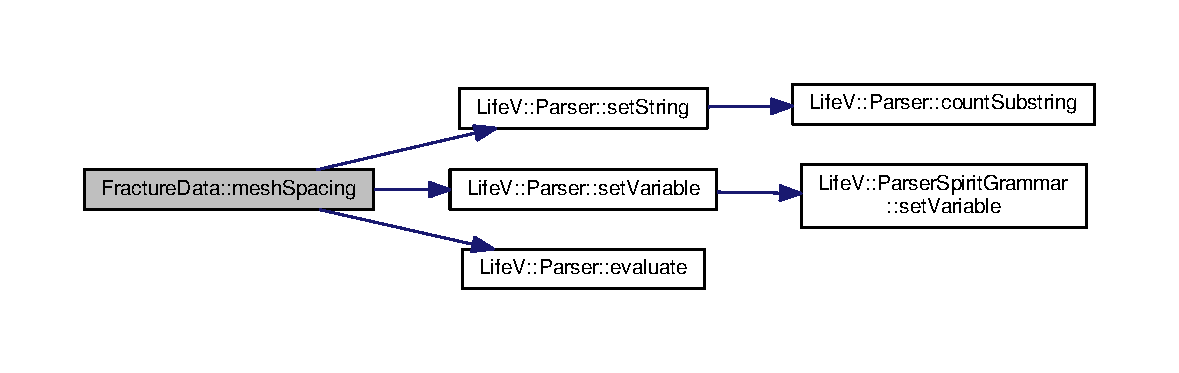
\includegraphics[width=350pt]{classFractureData_ab79d66dd830b6e1c55ade0d940c5c8cf_cgraph}
\end{center}
\end{figure}




Questo è il grafo dei chiamanti di questa funzione\-:
\nopagebreak
\begin{figure}[H]
\begin{center}
\leavevmode
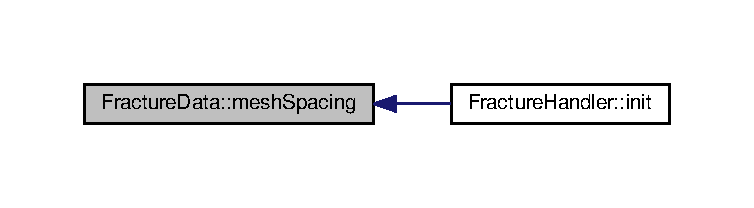
\includegraphics[width=350pt]{classFractureData_ab79d66dd830b6e1c55ade0d940c5c8cf_icgraph}
\end{center}
\end{figure}


\hypertarget{classFractureData_aab77ec8a8d3e878b5dfb72deb48841e7}{\index{Fracture\-Data@{Fracture\-Data}!porosity@{porosity}}
\index{porosity@{porosity}!FractureData@{Fracture\-Data}}
\subsubsection[{porosity}]{\setlength{\rightskip}{0pt plus 5cm}scalar\-\_\-type Fracture\-Data\-::porosity (
\begin{DoxyParamCaption}
\item[{const scalar\-\_\-type \&}]{u}
\end{DoxyParamCaption}
)}}\label{classFractureData_aab77ec8a8d3e878b5dfb72deb48841e7}

\begin{DoxyCode}
204 \{
205     M\_parser.\hyperlink{classLifeV_1_1Parser_ac05769e836a0dc95d9c020df361a5194}{setString}( M\_invP );
206     M\_parser.\hyperlink{classLifeV_1_1Parser_aa2b362e12b8feb60231705d499c9fbae}{setVariable} ( \textcolor{stringliteral}{"x"}, \hyperlink{confronto_8m_a6277e2a7446059985dc9bcf0a4ac1a8f}{u} );
207 
208     \textcolor{keywordflow}{return} M\_parser.\hyperlink{classLifeV_1_1Parser_a51d84fd4ae6d420620e7beee58fad673}{evaluate} ();
209 \}\textcolor{comment}{// porosity}
\end{DoxyCode}


Questo è il grafo delle chiamate per questa funzione\-:
\nopagebreak
\begin{figure}[H]
\begin{center}
\leavevmode
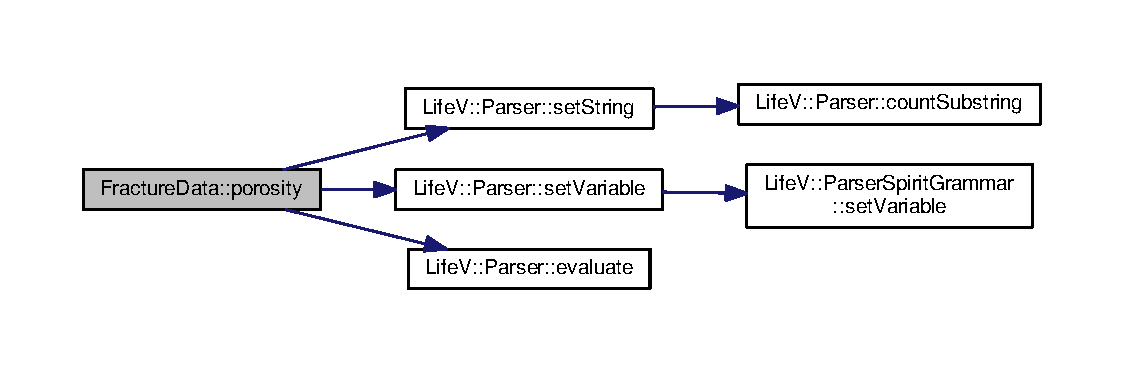
\includegraphics[width=350pt]{classFractureData_aab77ec8a8d3e878b5dfb72deb48841e7_cgraph}
\end{center}
\end{figure}




Questo è il grafo dei chiamanti di questa funzione\-:
\nopagebreak
\begin{figure}[H]
\begin{center}
\leavevmode
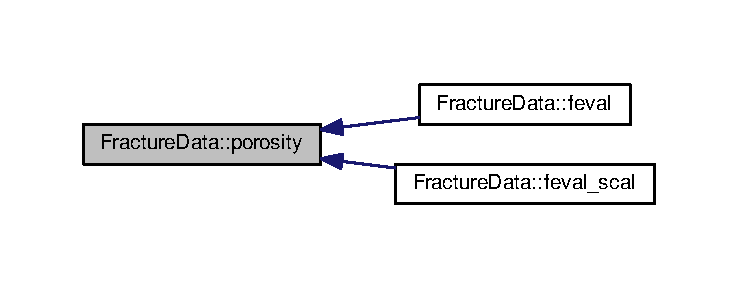
\includegraphics[width=350pt]{classFractureData_aab77ec8a8d3e878b5dfb72deb48841e7_icgraph}
\end{center}
\end{figure}


\hypertarget{classFractureData_a9598cf66a822a593e819df754420a2c2}{\index{Fracture\-Data@{Fracture\-Data}!velocity@{velocity}}
\index{velocity@{velocity}!FractureData@{Fracture\-Data}}
\subsubsection[{velocity}]{\setlength{\rightskip}{0pt plus 5cm}scalar\-\_\-type Fracture\-Data\-::velocity (
\begin{DoxyParamCaption}
\item[{const scalar\-\_\-type \&}]{u}
\end{DoxyParamCaption}
)}}\label{classFractureData_a9598cf66a822a593e819df754420a2c2}

\begin{DoxyCode}
195 \{
196     M\_parser.\hyperlink{classLifeV_1_1Parser_ac05769e836a0dc95d9c020df361a5194}{setString}( M\_U );
197     M\_parser.\hyperlink{classLifeV_1_1Parser_aa2b362e12b8feb60231705d499c9fbae}{setVariable} ( \textcolor{stringliteral}{"x"}, \hyperlink{confronto_8m_a6277e2a7446059985dc9bcf0a4ac1a8f}{u} );
198 
199     \textcolor{keywordflow}{return} M\_parser.\hyperlink{classLifeV_1_1Parser_a51d84fd4ae6d420620e7beee58fad673}{evaluate} ();
200 \}\textcolor{comment}{// velocity}
\end{DoxyCode}


Questo è il grafo delle chiamate per questa funzione\-:
\nopagebreak
\begin{figure}[H]
\begin{center}
\leavevmode
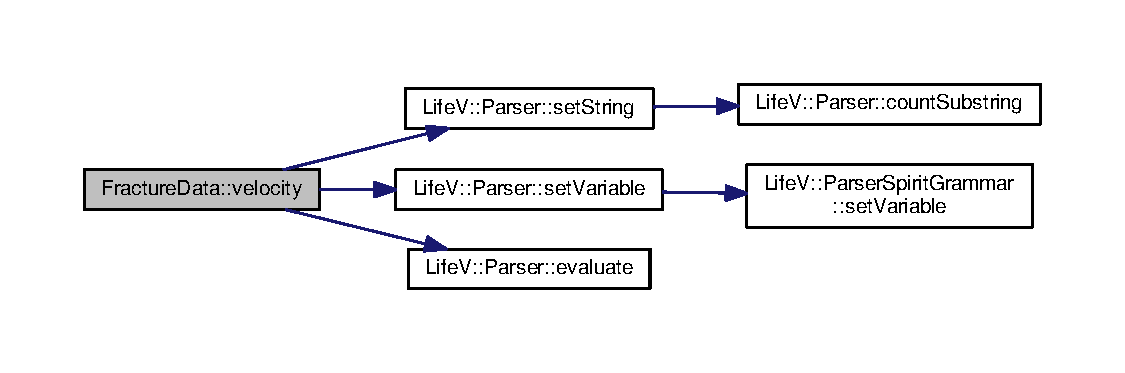
\includegraphics[width=350pt]{classFractureData_a9598cf66a822a593e819df754420a2c2_cgraph}
\end{center}
\end{figure}




Questo è il grafo dei chiamanti di questa funzione\-:
\nopagebreak
\begin{figure}[H]
\begin{center}
\leavevmode
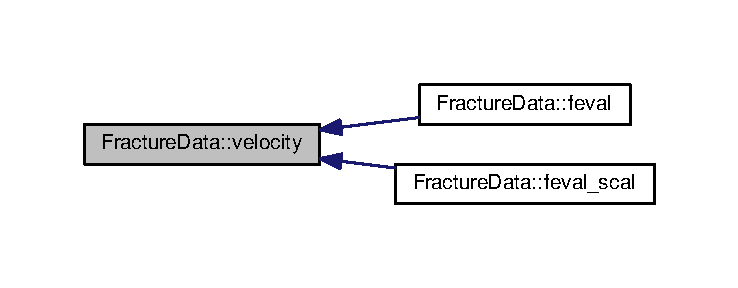
\includegraphics[width=350pt]{classFractureData_a9598cf66a822a593e819df754420a2c2_icgraph}
\end{center}
\end{figure}




La documentazione per questa classe è stata generata a partire dai seguenti file\-:\begin{DoxyCompactItemize}
\item 
include/\hyperlink{FractureData_8h}{Fracture\-Data.\-h}\item 
src/\hyperlink{FractureData_8cc}{Fracture\-Data.\-cc}\end{DoxyCompactItemize}

\hypertarget{classFractureHandler}{\section{Riferimenti per la classe Fracture\-Handler}
\label{classFractureHandler}\index{Fracture\-Handler@{Fracture\-Handler}}
}


{\ttfamily \#include $<$Fracture\-Handler.\-h$>$}

\subsection*{Membri pubblici}
\begin{DoxyCompactItemize}
\item 
\hyperlink{classFractureHandler_a75d39ff5fed50df17ab859eff0ff3958}{Fracture\-Handler} (const Get\-Pot \&data\-File, const size\-\_\-type I\-D, const \hyperlink{Exporter_8h_ac9d7f94fea8b91459a536bfaa2f3910c}{Exporter\-Ptr\-\_\-\-Type} \&exporter, const std\-::string \&section=\char`\"{}fracture\-Data/\char`\"{}, const std\-::string \&section\-Saturation=\char`\"{}saturation/\char`\"{})
\item 
void \hyperlink{classFractureHandler_aa28ce054ba2a2679214956c71f8cf1e0}{init} ()
\item 
void \hyperlink{classFractureHandler_a391031a951667a3d8b2f633602856ee3}{set\-Fracture\-Intersection} (const \hyperlink{Core_8h_a83c51913d041a5001e8683434c09857f}{size\-Vector\-\_\-\-Type} \&nodes, const \hyperlink{classFractureHandler}{Fracture\-Handler} \&fracture\-Involved)
\begin{DoxyCompactList}\small\item\em Funzione che definisce il nodo in cui la frattura corrente ha un'intersezione, e la frattura coinvolta. \end{DoxyCompactList}\item 
const size\-\_\-type \& \hyperlink{classFractureHandler_a439092fd58fa5d3295bffb71861cf7b9}{get\-I\-D} () const 
\item 
\hyperlink{classFractureData}{Fracture\-Data} \& \hyperlink{classFractureHandler_a68ed77a8d9816a472700ee4bcf2f505d}{get\-Data} ()
\item 
\hyperlink{LevelSetHandler_8h_aba343569cb3213c103252f69c39cad0b}{Level\-Set\-Handler\-Ptr\-\_\-\-Type} \& \hyperlink{classFractureHandler_af37ab12a17f812a960da2aa71699ba0f}{get\-Level\-Set} ()
\item 
const getfem\-::mesh \& \hyperlink{classFractureHandler_ac46642070f0dc03d8db9ef1844129f74}{get\-Mesh} () const 
\item 
getfem\-::mesh \& \hyperlink{classFractureHandler_a49fae167e260a823281daabb25310719}{get\-Mesh} ()
\item 
const getfem\-::mesh \& \hyperlink{classFractureHandler_a9ff9f584b850d6b750981befdbefbdbe}{get\-Mesh\-Flat} () const 
\item 
getfem\-::mesh \& \hyperlink{classFractureHandler_ad9b02a825d444016b3ab8ee901f887f6}{get\-Mesh\-Flat} ()
\item 
\hyperlink{Core_8h_a4e75b5863535ba1dd79942de2846eff0}{scalar\-Vector\-\_\-\-Type} \hyperlink{classFractureHandler_adf60ff829fe91638051bc94520869d2c}{get\-Ci} () const 
\item 
void \hyperlink{classFractureHandler_a002e255a1976918ffbe6ea63b0fdae1b}{num\-Fractures} (const size\-\_\-type \&num\-Fractures)
\end{DoxyCompactItemize}


\subsection{Documentazione dei costruttori e dei distruttori}
\hypertarget{classFractureHandler_a75d39ff5fed50df17ab859eff0ff3958}{\index{Fracture\-Handler@{Fracture\-Handler}!Fracture\-Handler@{Fracture\-Handler}}
\index{Fracture\-Handler@{Fracture\-Handler}!FractureHandler@{Fracture\-Handler}}
\subsubsection[{Fracture\-Handler}]{\setlength{\rightskip}{0pt plus 5cm}Fracture\-Handler\-::\-Fracture\-Handler (
\begin{DoxyParamCaption}
\item[{const Get\-Pot \&}]{data\-File, }
\item[{const size\-\_\-type}]{I\-D, }
\item[{const {\bf Exporter\-Ptr\-\_\-\-Type} \&}]{exporter, }
\item[{const std\-::string \&}]{section = {\ttfamily \char`\"{}fractureData/\char`\"{}}, }
\item[{const std\-::string \&}]{section\-Saturation = {\ttfamily \char`\"{}saturation/\char`\"{}}}
\end{DoxyParamCaption}
)}}\label{classFractureHandler_a75d39ff5fed50df17ab859eff0ff3958}

\begin{DoxyCode}
13                                                                       :
14                                    M\_ID( \hyperlink{namespaceLifeV_a7c0e64679fcd30daa5471b87a57601e9}{ID} ),
15                                    M\_data( dataFile, section ),
16                                    M\_exporter ( exporter )
17 \{
18     M\_levelSet.reset( \textcolor{keyword}{new} \hyperlink{classLevelSetHandler}{LevelSetHandler\_Type} ( dataFile, section ) );
19 
20 \}\textcolor{comment}{// costruttore}
\end{DoxyCode}


\subsection{Documentazione delle funzioni membro}
\hypertarget{classFractureHandler_adf60ff829fe91638051bc94520869d2c}{\index{Fracture\-Handler@{Fracture\-Handler}!get\-Ci@{get\-Ci}}
\index{get\-Ci@{get\-Ci}!FractureHandler@{Fracture\-Handler}}
\subsubsection[{get\-Ci}]{\setlength{\rightskip}{0pt plus 5cm}{\bf scalar\-Vector\-\_\-\-Type} Fracture\-Handler\-::get\-Ci (
\begin{DoxyParamCaption}
{}
\end{DoxyParamCaption}
) const\hspace{0.3cm}{\ttfamily [inline]}}}\label{classFractureHandler_adf60ff829fe91638051bc94520869d2c}

\begin{DoxyCode}
82     \{
83         \textcolor{keywordflow}{return} M\_ci;
84     \}
\end{DoxyCode}
\hypertarget{classFractureHandler_a68ed77a8d9816a472700ee4bcf2f505d}{\index{Fracture\-Handler@{Fracture\-Handler}!get\-Data@{get\-Data}}
\index{get\-Data@{get\-Data}!FractureHandler@{Fracture\-Handler}}
\subsubsection[{get\-Data}]{\setlength{\rightskip}{0pt plus 5cm}{\bf Fracture\-Data}\& Fracture\-Handler\-::get\-Data (
\begin{DoxyParamCaption}
{}
\end{DoxyParamCaption}
)\hspace{0.3cm}{\ttfamily [inline]}}}\label{classFractureHandler_a68ed77a8d9816a472700ee4bcf2f505d}

\begin{DoxyCode}
50     \{
51         \textcolor{keywordflow}{return} M\_data;
52     \}
\end{DoxyCode}
\hypertarget{classFractureHandler_a439092fd58fa5d3295bffb71861cf7b9}{\index{Fracture\-Handler@{Fracture\-Handler}!get\-I\-D@{get\-I\-D}}
\index{get\-I\-D@{get\-I\-D}!FractureHandler@{Fracture\-Handler}}
\subsubsection[{get\-I\-D}]{\setlength{\rightskip}{0pt plus 5cm}const size\-\_\-type\& Fracture\-Handler\-::get\-I\-D (
\begin{DoxyParamCaption}
{}
\end{DoxyParamCaption}
) const\hspace{0.3cm}{\ttfamily [inline]}}}\label{classFractureHandler_a439092fd58fa5d3295bffb71861cf7b9}

\begin{DoxyCode}
45     \{
46         \textcolor{keywordflow}{return} M\_ID;
47     \}
\end{DoxyCode}


Questo è il grafo dei chiamanti di questa funzione\-:
\nopagebreak
\begin{figure}[H]
\begin{center}
\leavevmode
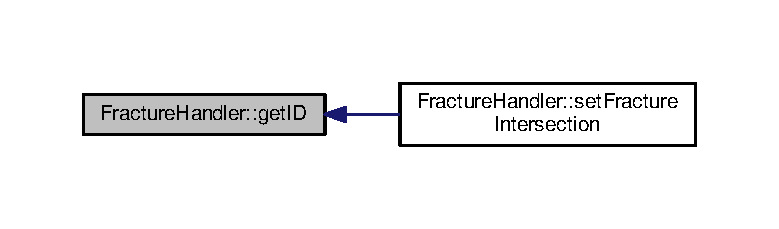
\includegraphics[width=350pt]{classFractureHandler_a439092fd58fa5d3295bffb71861cf7b9_icgraph}
\end{center}
\end{figure}


\hypertarget{classFractureHandler_af37ab12a17f812a960da2aa71699ba0f}{\index{Fracture\-Handler@{Fracture\-Handler}!get\-Level\-Set@{get\-Level\-Set}}
\index{get\-Level\-Set@{get\-Level\-Set}!FractureHandler@{Fracture\-Handler}}
\subsubsection[{get\-Level\-Set}]{\setlength{\rightskip}{0pt plus 5cm}{\bf Level\-Set\-Handler\-Ptr\-\_\-\-Type}\& Fracture\-Handler\-::get\-Level\-Set (
\begin{DoxyParamCaption}
{}
\end{DoxyParamCaption}
)\hspace{0.3cm}{\ttfamily [inline]}}}\label{classFractureHandler_af37ab12a17f812a960da2aa71699ba0f}

\begin{DoxyCode}
55     \{
56         \textcolor{keywordflow}{return} M\_levelSet;
57     \}
\end{DoxyCode}
\hypertarget{classFractureHandler_ac46642070f0dc03d8db9ef1844129f74}{\index{Fracture\-Handler@{Fracture\-Handler}!get\-Mesh@{get\-Mesh}}
\index{get\-Mesh@{get\-Mesh}!FractureHandler@{Fracture\-Handler}}
\subsubsection[{get\-Mesh}]{\setlength{\rightskip}{0pt plus 5cm}const getfem\-::mesh\& Fracture\-Handler\-::get\-Mesh (
\begin{DoxyParamCaption}
{}
\end{DoxyParamCaption}
) const\hspace{0.3cm}{\ttfamily [inline]}}}\label{classFractureHandler_ac46642070f0dc03d8db9ef1844129f74}

\begin{DoxyCode}
60     \{
61         \textcolor{keywordflow}{return} M\_mesh;
62     \}
\end{DoxyCode}
\hypertarget{classFractureHandler_a49fae167e260a823281daabb25310719}{\index{Fracture\-Handler@{Fracture\-Handler}!get\-Mesh@{get\-Mesh}}
\index{get\-Mesh@{get\-Mesh}!FractureHandler@{Fracture\-Handler}}
\subsubsection[{get\-Mesh}]{\setlength{\rightskip}{0pt plus 5cm}getfem\-::mesh\& Fracture\-Handler\-::get\-Mesh (
\begin{DoxyParamCaption}
{}
\end{DoxyParamCaption}
)\hspace{0.3cm}{\ttfamily [inline]}}}\label{classFractureHandler_a49fae167e260a823281daabb25310719}

\begin{DoxyCode}
66     \{
67         \textcolor{keywordflow}{return} M\_mesh;
68     \}
\end{DoxyCode}
\hypertarget{classFractureHandler_a9ff9f584b850d6b750981befdbefbdbe}{\index{Fracture\-Handler@{Fracture\-Handler}!get\-Mesh\-Flat@{get\-Mesh\-Flat}}
\index{get\-Mesh\-Flat@{get\-Mesh\-Flat}!FractureHandler@{Fracture\-Handler}}
\subsubsection[{get\-Mesh\-Flat}]{\setlength{\rightskip}{0pt plus 5cm}const getfem\-::mesh\& Fracture\-Handler\-::get\-Mesh\-Flat (
\begin{DoxyParamCaption}
{}
\end{DoxyParamCaption}
) const\hspace{0.3cm}{\ttfamily [inline]}}}\label{classFractureHandler_a9ff9f584b850d6b750981befdbefbdbe}

\begin{DoxyCode}
71     \{
72         \textcolor{keywordflow}{return} M\_meshFlat;
73     \}
\end{DoxyCode}
\hypertarget{classFractureHandler_ad9b02a825d444016b3ab8ee901f887f6}{\index{Fracture\-Handler@{Fracture\-Handler}!get\-Mesh\-Flat@{get\-Mesh\-Flat}}
\index{get\-Mesh\-Flat@{get\-Mesh\-Flat}!FractureHandler@{Fracture\-Handler}}
\subsubsection[{get\-Mesh\-Flat}]{\setlength{\rightskip}{0pt plus 5cm}getfem\-::mesh\& Fracture\-Handler\-::get\-Mesh\-Flat (
\begin{DoxyParamCaption}
{}
\end{DoxyParamCaption}
)\hspace{0.3cm}{\ttfamily [inline]}}}\label{classFractureHandler_ad9b02a825d444016b3ab8ee901f887f6}

\begin{DoxyCode}
77     \{
78         \textcolor{keywordflow}{return} M\_meshFlat;
79     \}
\end{DoxyCode}
\hypertarget{classFractureHandler_aa28ce054ba2a2679214956c71f8cf1e0}{\index{Fracture\-Handler@{Fracture\-Handler}!init@{init}}
\index{init@{init}!FractureHandler@{Fracture\-Handler}}
\subsubsection[{init}]{\setlength{\rightskip}{0pt plus 5cm}void Fracture\-Handler\-::init (
\begin{DoxyParamCaption}
{}
\end{DoxyParamCaption}
)}}\label{classFractureHandler_aa28ce054ba2a2679214956c71f8cf1e0}

\begin{DoxyCode}
25 \{
26     \textcolor{comment}{// Geometric transformation usign primal finite elements type in the fracture}
27     M\_geometricTransformation = bgeot::geometric\_trans\_descriptor( M\_data.
      \hyperlink{classFractureData_aaded6c0452470489beb4ab95b5f4158f}{getMeshType}() );
28 
29 
30     \textcolor{comment}{//-------------------- M\_meshFlat, mesh sul piano orizzontale --------------------//}
31 
32     \textcolor{comment}{// costruisco una mesh standard, l'idea di mantenere una mesh 1d sul piano orizzontale è solo per
       comodità}
33 
34     \hyperlink{Core_8h_a83c51913d041a5001e8683434c09857f}{sizeVector\_Type} fractureNumberSubdivision( M\_data.
      \hyperlink{classFractureData_a4b310767d1a91b0cef404093aacfab82}{getSpaceDimension}() );
35 
36     std::fill( fractureNumberSubdivision.begin(), fractureNumberSubdivision.end(), M\_data.
      \hyperlink{classFractureData_aeb3c6a78af1e2746bf5ce69c9ae8945d}{getSpatialDiscretization}() );
37 
38     getfem::regular\_unit\_mesh( M\_meshFlat, fractureNumberSubdivision, M\_geometricTransformation );
39 
40     bgeot::base\_matrix fractureTransformMatrix( M\_data.\hyperlink{classFractureData_a4b310767d1a91b0cef404093aacfab82}{getSpaceDimension}(), M\_data.
      \hyperlink{classFractureData_a4b310767d1a91b0cef404093aacfab82}{getSpaceDimension}() );
41 
42     \hyperlink{Core_8h_a4e75b5863535ba1dd79942de2846eff0}{scalarVector\_Type} fractureLength(3);
43     fractureLength [ 0 ] = M\_data.\hyperlink{classFractureData_abaebcf16d83713858e25837939ad3161}{getLengthAbscissa}();
44     fractureLength [ 1 ] = M\_data.\hyperlink{classFractureData_a905e953f685b1329ddcc7ee56f8302b1}{getLengthOrdinate}();
45     fractureLength [ 2 ] = M\_data.\hyperlink{classFractureData_a79747fff53da9d858950d83ad0114288}{getLengthQuota}();
46 
47     \textcolor{keywordflow}{for} ( size\_type \hyperlink{god__e_8m_a8604be5925f4266ab5ccc69675329c80}{i} = 0; \hyperlink{god__e_8m_a8604be5925f4266ab5ccc69675329c80}{i} < M\_data.\hyperlink{classFractureData_a4b310767d1a91b0cef404093aacfab82}{getSpaceDimension}(); ++
      \hyperlink{god__e_8m_a8604be5925f4266ab5ccc69675329c80}{i} )
48     \{
49         fractureTransformMatrix(\hyperlink{god__e_8m_a8604be5925f4266ab5ccc69675329c80}{i}, \hyperlink{god__e_8m_a8604be5925f4266ab5ccc69675329c80}{i}) = (\hyperlink{god__e_8m_a8604be5925f4266ab5ccc69675329c80}{i} < M\_data.\hyperlink{classFractureData_a4b310767d1a91b0cef404093aacfab82}{getSpaceDimension}()) ? 
      fractureLength [ \hyperlink{god__e_8m_a8604be5925f4266ab5ccc69675329c80}{i} ] : 1.0;
50     \}
51 
52     \textcolor{comment}{// riscalo la mesh unitaria M\_mediumMesh to [M\_lengthAbscissa,M\_lengthOrdinate]}
53     M\_meshFlat.transformation( fractureTransformMatrix );
54     \textcolor{keywordflow}{for} ( size\_type \hyperlink{god__e_8m_a8604be5925f4266ab5ccc69675329c80}{i} = 0; \hyperlink{god__e_8m_a8604be5925f4266ab5ccc69675329c80}{i} < M\_meshFlat.points().size(); ++\hyperlink{god__e_8m_a8604be5925f4266ab5ccc69675329c80}{i} )
55     \{
56         M\_meshFlat.points() [ \hyperlink{god__e_8m_a8604be5925f4266ab5ccc69675329c80}{i} ] [ 0 ] = M\_data.\hyperlink{classFractureData_ab79d66dd830b6e1c55ade0d940c5c8cf}{meshSpacing}( M\_meshFlat.points() [ 
      \hyperlink{god__e_8m_a8604be5925f4266ab5ccc69675329c80}{i} ] [ 0 ] );
57     \}
58 
59 
60     \textcolor{comment}{//-------------------- M\_mesh, mesh reale nel piano 2d --------------------//}
61     \textcolor{comment}{//costruisco la M\_mediumMesh n.2 quella di servizio, quella della frattura mappata}
62 
63 
64 
65     \hyperlink{Core_8h_a83c51913d041a5001e8683434c09857f}{sizeVector\_Type} ind( M\_meshFlat.points().size() );
66     \textcolor{keywordflow}{for} ( size\_type \hyperlink{god__e_8m_a8604be5925f4266ab5ccc69675329c80}{i} = 0; \hyperlink{god__e_8m_a8604be5925f4266ab5ccc69675329c80}{i} < M\_meshFlat.points().size(); ++\hyperlink{god__e_8m_a8604be5925f4266ab5ccc69675329c80}{i} )
67     \{
68         bgeot::base\_node P(M\_data.\hyperlink{classFractureData_a4b310767d1a91b0cef404093aacfab82}{getSpaceDimension}() + 2);
69         bgeot::base\_node P1(M\_data.\hyperlink{classFractureData_a4b310767d1a91b0cef404093aacfab82}{getSpaceDimension}() + 2);
70 
71         scalar\_type \hyperlink{discontinuo_8m_aaccc9105df5383111407fd5b41255e23}{t} = \hyperlink{god__e_8m_a8604be5925f4266ab5ccc69675329c80}{i}*1./(M\_data.\hyperlink{classFractureData_aeb3c6a78af1e2746bf5ce69c9ae8945d}{getSpatialDiscretization} () );
72 
73         P1 [ 0 ] = \hyperlink{discontinuo_8m_aaccc9105df5383111407fd5b41255e23}{t};
74 
75         P [ 0 ] = P1 [ 0 ];
76         P [ 1 ] =  M\_levelSet->getData()->y\_map( P1 );
77         ind [ \hyperlink{god__e_8m_a8604be5925f4266ab5ccc69675329c80}{i} ] = M\_mesh.add\_point( P );
78     \}
79 
80 
81 
82     \textcolor{keywordflow}{for} ( size\_type \hyperlink{god__e_8m_a8604be5925f4266ab5ccc69675329c80}{i} = 0; \hyperlink{god__e_8m_a8604be5925f4266ab5ccc69675329c80}{i} < M\_meshFlat.convex\_index().size(); ++\hyperlink{god__e_8m_a8604be5925f4266ab5ccc69675329c80}{i} )
83     \{
84         std::vector<bgeot::size\_type> point(3);
85         point [ 0 ] = M\_meshFlat.ind\_points\_of\_convex(\hyperlink{god__e_8m_a8604be5925f4266ab5ccc69675329c80}{i}) [ 0 ];
86         point [ 1 ] = M\_meshFlat.ind\_points\_of\_convex(\hyperlink{god__e_8m_a8604be5925f4266ab5ccc69675329c80}{i}) [ 1 ];
87         point [ 2 ] = M\_meshFlat.ind\_points\_of\_convex(\hyperlink{god__e_8m_a8604be5925f4266ab5ccc69675329c80}{i}) [ 2 ];
88 
89         M\_mesh.add\_convex( M\_geometricTransformation, point.begin() );
90     \}
91 
92     \textcolor{comment}{// inizializzo M\_ci, condizione iniziale}
93     M\_ci.resize( M\_data.\hyperlink{classFractureData_aeb3c6a78af1e2746bf5ce69c9ae8945d}{getSpatialDiscretization}() - 1 );
94 
95 
96 
97     \textcolor{keywordflow}{for} ( size\_type \hyperlink{god__e_8m_a8604be5925f4266ab5ccc69675329c80}{i} = 0; \hyperlink{god__e_8m_a8604be5925f4266ab5ccc69675329c80}{i} < M\_data.\hyperlink{classFractureData_aeb3c6a78af1e2746bf5ce69c9ae8945d}{getSpatialDiscretization}() - 1; 
      \hyperlink{god__e_8m_a8604be5925f4266ab5ccc69675329c80}{i}++ )
98     \{
99         bgeot::basic\_mesh::ref\_mesh\_pt\_ct nodes = M\_meshFlat.points\_of\_convex ( 
      \hyperlink{god__e_8m_a8604be5925f4266ab5ccc69675329c80}{i} );
100 
101         scalar\_type \hyperlink{confronto_8m_ad2e52d4a42a755ccd73c8de47175afa3}{x} = nodes [ 0 ] [ 0 ];
102 
103         M\_ci [ \hyperlink{god__e_8m_a8604be5925f4266ab5ccc69675329c80}{i} ] = M\_data.\hyperlink{classFractureData_a142a1bb428365b60ed002362ca566517}{getCi}( x );
104     \}
105 
106     std::ostringstream ss;
107     ss << \textcolor{stringliteral}{"./matlab/risultati/inizialSaturation\_"} << M\_ID << \textcolor{stringliteral}{".txt"};
108 
109     std::string name = ss.str();
110 
111     std::ofstream exp( name );
112 
113     exp << M\_ci;
114 
115     \textcolor{keywordflow}{return};
116 \}\textcolor{comment}{// init}
\end{DoxyCode}


Questo è il grafo delle chiamate per questa funzione\-:
\nopagebreak
\begin{figure}[H]
\begin{center}
\leavevmode
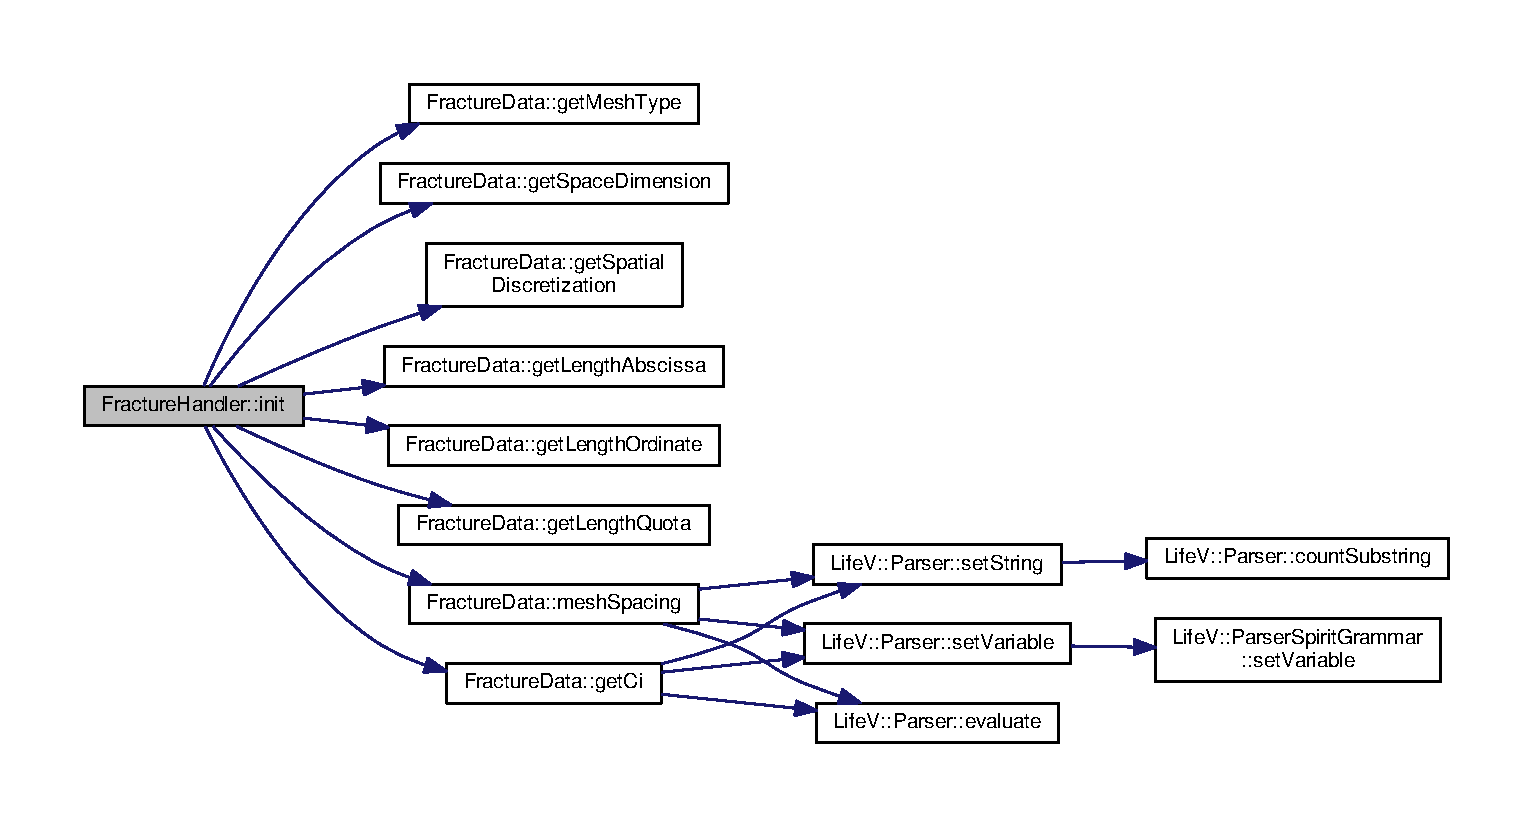
\includegraphics[width=350pt]{classFractureHandler_aa28ce054ba2a2679214956c71f8cf1e0_cgraph}
\end{center}
\end{figure}


\hypertarget{classFractureHandler_a002e255a1976918ffbe6ea63b0fdae1b}{\index{Fracture\-Handler@{Fracture\-Handler}!num\-Fractures@{num\-Fractures}}
\index{num\-Fractures@{num\-Fractures}!FractureHandler@{Fracture\-Handler}}
\subsubsection[{num\-Fractures}]{\setlength{\rightskip}{0pt plus 5cm}void Fracture\-Handler\-::num\-Fractures (
\begin{DoxyParamCaption}
\item[{const size\-\_\-type \&}]{num\-Fractures}
\end{DoxyParamCaption}
)\hspace{0.3cm}{\ttfamily [inline]}}}\label{classFractureHandler_a002e255a1976918ffbe6ea63b0fdae1b}

\begin{DoxyCode}
87     \{
88         M\_fractureIntersectElements.resize ( \hyperlink{classFractureHandler_a002e255a1976918ffbe6ea63b0fdae1b}{numFractures} );
89         M\_fractureIntersectElementsGlobalIndex.resize ( \hyperlink{classFractureHandler_a002e255a1976918ffbe6ea63b0fdae1b}{numFractures} );
90     \}
\end{DoxyCode}
\hypertarget{classFractureHandler_a391031a951667a3d8b2f633602856ee3}{\index{Fracture\-Handler@{Fracture\-Handler}!set\-Fracture\-Intersection@{set\-Fracture\-Intersection}}
\index{set\-Fracture\-Intersection@{set\-Fracture\-Intersection}!FractureHandler@{Fracture\-Handler}}
\subsubsection[{set\-Fracture\-Intersection}]{\setlength{\rightskip}{0pt plus 5cm}void Fracture\-Handler\-::set\-Fracture\-Intersection (
\begin{DoxyParamCaption}
\item[{const {\bf size\-Vector\-\_\-\-Type} \&}]{nodes, }
\item[{const {\bf Fracture\-Handler} \&}]{fracture\-Involved}
\end{DoxyParamCaption}
)}}\label{classFractureHandler_a391031a951667a3d8b2f633602856ee3}


Funzione che definisce il nodo in cui la frattura corrente ha un'intersezione, e la frattura coinvolta. 


\begin{DoxyCode}
120 \{
121     size\_type otherFractureID = fractureInvolved.\hyperlink{classFractureHandler_a439092fd58fa5d3295bffb71861cf7b9}{getID}();
122 
123     M\_fractureIntersectElements[ otherFractureID ].push\_back( nodes[ 0 ] );
124 
125     \textcolor{keywordflow}{return};
126 \}\textcolor{comment}{// setFractureIntersection}
\end{DoxyCode}


Questo è il grafo delle chiamate per questa funzione\-:
\nopagebreak
\begin{figure}[H]
\begin{center}
\leavevmode
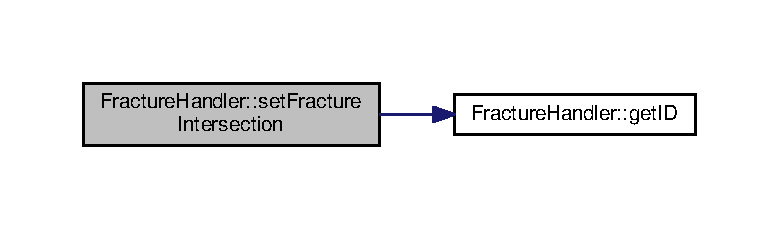
\includegraphics[width=350pt]{classFractureHandler_a391031a951667a3d8b2f633602856ee3_cgraph}
\end{center}
\end{figure}




La documentazione per questa classe è stata generata a partire dai seguenti file\-:\begin{DoxyCompactItemize}
\item 
include/\hyperlink{FractureHandler_8h}{Fracture\-Handler.\-h}\item 
src/\hyperlink{FractureHandler_8cc}{Fracture\-Handler.\-cc}\end{DoxyCompactItemize}

\hypertarget{classFractureIntersect}{\section{Riferimenti per la classe Fracture\-Intersect}
\label{classFractureIntersect}\index{Fracture\-Intersect@{Fracture\-Intersect}}
}


{\ttfamily \#include $<$Fracture\-Intersect.\-h$>$}

\subsection*{Membri pubblici}
\begin{DoxyCompactItemize}
\item 
\hyperlink{classFractureIntersect_a2416c29105bde5cbf9032b04db47ba31}{Fracture\-Intersect} ()
\item 
void \hyperlink{classFractureIntersect_a192d02d60bcab84e6ab2765c8167f614}{construct\-Intesection} (const \hyperlink{FractureHandler_8h_a2f0b57e18ecf89912d7de0c87158009e}{Fracture\-Ptr\-Container\-\_\-\-Type} \&fractures)
\begin{DoxyCompactList}\small\item\em Con questa funzione costruisco la classe che contiene tutte le intersezioni valutando, per ogni frattura singolarmente, se esiste un punto in comune con le altre. \end{DoxyCompactList}\item 
void \hyperlink{classFractureIntersect_a63e99fbb20ef4804cbf99d8f1ab19ac6}{find\-Intersection} (const \hyperlink{FractureHandler_8h_af23fb7a30aaff864bd42587af4f1e78a}{Fracture\-Handler\-Ptr\-\_\-\-Type} \&\hyperlink{god__e_8m_a8ea372f7ee3c01d11fc4b4d13b8e6a75}{f}, const \hyperlink{FractureHandler_8h_a2f0b57e18ecf89912d7de0c87158009e}{Fracture\-Ptr\-Container\-\_\-\-Type} \&fractures, \hyperlink{Core_8h_a83c51913d041a5001e8683434c09857f}{size\-Vector\-\_\-\-Type} \&nodes, \hyperlink{Core_8h_a83c51913d041a5001e8683434c09857f}{size\-Vector\-\_\-\-Type} \&list\-Of\-Fractures)
\begin{DoxyCompactList}\small\item\em Con questa funzione verifico se una data frattura ha intersezione con tutte le altre. \end{DoxyCompactList}\item 
void \hyperlink{classFractureIntersect_a01bc187a846208a47a13daeeb94b13f5}{push\-\_\-back} (const \hyperlink{classIntersectData}{Intersect\-Data} \&intersection)
\begin{DoxyCompactList}\small\item\em Dopo aver costruito una nuova intersezione, prima di inserirla nel vettore delle intersezioni, verifico che non vi sia già. \end{DoxyCompactList}\item 
\hyperlink{IntersectData_8h_a822ec3b760dfb603e1cf0bfe3ad5636a}{Intersect\-Data\-Container\-\_\-\-Type} \hyperlink{classFractureIntersect_a248df8f326f844e34d807234efdfd693}{get\-Cross\-Intersections} () const 
\begin{DoxyCompactList}\small\item\em Funzione che restituisce tutte le intersezioni di tipo \char`\"{} Cross \char`\"{}. \end{DoxyCompactList}\item 
\hyperlink{IntersectData_8h_a822ec3b760dfb603e1cf0bfe3ad5636a}{Intersect\-Data\-Container\-\_\-\-Type} \hyperlink{classFractureIntersect_a18ff664767b7e8ffa876b80a6100e74d}{get\-Bifurcation\-Intersections} () const 
\begin{DoxyCompactList}\small\item\em Funzione che restituisce tutte le intersezioni di tipo \char`\"{} Bifurcation \char`\"{}. \end{DoxyCompactList}\item 
size\-\_\-type \hyperlink{classFractureIntersect_a8d9f707319b9b83744b6e03f19003734}{get\-Number\-Cross} () const 
\item 
size\-\_\-type \hyperlink{classFractureIntersect_afba7c92096a4b92a27fcb4f1158c7279}{get\-Number\-Bifurcation} () const 
\end{DoxyCompactItemize}


\subsection{Documentazione dei costruttori e dei distruttori}
\hypertarget{classFractureIntersect_a2416c29105bde5cbf9032b04db47ba31}{\index{Fracture\-Intersect@{Fracture\-Intersect}!Fracture\-Intersect@{Fracture\-Intersect}}
\index{Fracture\-Intersect@{Fracture\-Intersect}!FractureIntersect@{Fracture\-Intersect}}
\subsubsection[{Fracture\-Intersect}]{\setlength{\rightskip}{0pt plus 5cm}Fracture\-Intersect\-::\-Fracture\-Intersect (
\begin{DoxyParamCaption}
{}
\end{DoxyParamCaption}
)\hspace{0.3cm}{\ttfamily [inline]}}}\label{classFractureIntersect_a2416c29105bde5cbf9032b04db47ba31}

\begin{DoxyCode}
31     \{\};
\end{DoxyCode}


\subsection{Documentazione delle funzioni membro}
\hypertarget{classFractureIntersect_a192d02d60bcab84e6ab2765c8167f614}{\index{Fracture\-Intersect@{Fracture\-Intersect}!construct\-Intesection@{construct\-Intesection}}
\index{construct\-Intesection@{construct\-Intesection}!FractureIntersect@{Fracture\-Intersect}}
\subsubsection[{construct\-Intesection}]{\setlength{\rightskip}{0pt plus 5cm}void Fracture\-Intersect\-::construct\-Intesection (
\begin{DoxyParamCaption}
\item[{const {\bf Fracture\-Ptr\-Container\-\_\-\-Type} \&}]{fractures}
\end{DoxyParamCaption}
)}}\label{classFractureIntersect_a192d02d60bcab84e6ab2765c8167f614}


Con questa funzione costruisco la classe che contiene tutte le intersezioni valutando, per ogni frattura singolarmente, se esiste un punto in comune con le altre. 

Poichè le fratture sono definite come segmenti non tagliati, le intersezioni tra fratture possono trovarsi solo a inizio o fine frattura 
\begin{DoxyCode}
10 \{
11     size\_type numberFractures = fractures.size();
12 
13     \hyperlink{Core_8h_a80e8381d86ecb0a7f4f87ff84d1a0be5}{sizeVectorContainer\_Type} nodes ( numberFractures );
14     \hyperlink{Core_8h_a80e8381d86ecb0a7f4f87ff84d1a0be5}{sizeVectorContainer\_Type} listOfFractures ( numberFractures );
15 
16     \textcolor{comment}{/*}
17 \textcolor{comment}{     * per ogni frattura cerco le intersezioni con le altre e aggiungo l'informazione che si intersecano}
18 \textcolor{comment}{     */}
19     \textcolor{keywordflow}{for} ( size\_type \hyperlink{god__e_8m_a68f477f9b30a6300d5af9b02eac82f35}{f} = 0; \hyperlink{god__e_8m_a68f477f9b30a6300d5af9b02eac82f35}{f} < numberFractures; \hyperlink{god__e_8m_a68f477f9b30a6300d5af9b02eac82f35}{f}++ )
20     \{
21         \hyperlink{classFractureIntersect_a63e99fbb20ef4804cbf99d8f1ab19ac6}{findIntersection} ( fractures [ \hyperlink{god__e_8m_a68f477f9b30a6300d5af9b02eac82f35}{f} ], fractures, nodes [ f ],  listOfFractures [ f ]
       );
22 
23         \hyperlink{FractureHandler_8h_a2f0b57e18ecf89912d7de0c87158009e}{FracturePtrContainer\_Type} fracturesInvolved ( listOfFractures[ 
      \hyperlink{god__e_8m_a68f477f9b30a6300d5af9b02eac82f35}{f} ].size() +1 );
24 
25         fracturesInvolved[ 0 ] = fractures [ \hyperlink{god__e_8m_a68f477f9b30a6300d5af9b02eac82f35}{f} ];
26 
27         \textcolor{keywordflow}{for} ( size\_type j = 1; j < fracturesInvolved.size(); ++j )
28         \{
29              fracturesInvolved [ j ] = fractures [ listOfFractures [ \hyperlink{god__e_8m_a68f477f9b30a6300d5af9b02eac82f35}{f} ] [ j-1 ] ];
30         \}
31 
32         \textcolor{keywordflow}{if} ( nodes[ \hyperlink{god__e_8m_a68f477f9b30a6300d5af9b02eac82f35}{f} ].size() != 0 )
33         \{
34             \textcolor{keywordflow}{for} ( size\_type \hyperlink{god__e_8m_a8604be5925f4266ab5ccc69675329c80}{i} = 1; \hyperlink{god__e_8m_a8604be5925f4266ab5ccc69675329c80}{i} < fracturesInvolved.size(); \hyperlink{god__e_8m_a8604be5925f4266ab5ccc69675329c80}{i}++ )
35             \{
36                 fracturesInvolved[ \hyperlink{god__e_8m_a68f477f9b30a6300d5af9b02eac82f35}{f} ]->setFractureIntersection ( nodes [ \hyperlink{god__e_8m_a68f477f9b30a6300d5af9b02eac82f35}{f} ], *fracturesInvolved[ 
      \hyperlink{god__e_8m_a8604be5925f4266ab5ccc69675329c80}{i} ] );
37             \}
38         \}
39     \}
40 
41     \textcolor{comment}{/*}
42 \textcolor{comment}{     * ora che so quali sono le fratture che si intersecano e dove posso costruire le intersezioni}
43 \textcolor{comment}{     */}
44     \textcolor{keywordflow}{for} ( size\_type \hyperlink{god__e_8m_a8604be5925f4266ab5ccc69675329c80}{i} = 0; \hyperlink{god__e_8m_a8604be5925f4266ab5ccc69675329c80}{i} < nodes.size(); \hyperlink{god__e_8m_a8604be5925f4266ab5ccc69675329c80}{i}++ )
45     \{
46         \textcolor{keywordflow}{if} ( nodes [ \hyperlink{god__e_8m_a8604be5925f4266ab5ccc69675329c80}{i} ].size() != 0 )
47         \{
48             \textcolor{comment}{// Prendo i puntatori alle fratture coinvolte}
49             \hyperlink{FractureHandler_8h_a2f0b57e18ecf89912d7de0c87158009e}{FracturePtrContainer\_Type} fracturesInvolved ( listOfFractures[ 
      \hyperlink{god__e_8m_a8604be5925f4266ab5ccc69675329c80}{i} ].size() +1 );
50 
51             fracturesInvolved[ 0 ] = fractures[ \hyperlink{god__e_8m_a8604be5925f4266ab5ccc69675329c80}{i} ];
52 
53             \textcolor{keywordflow}{for} ( size\_type \hyperlink{god__e_8m_a68f477f9b30a6300d5af9b02eac82f35}{f} = 1; \hyperlink{god__e_8m_a68f477f9b30a6300d5af9b02eac82f35}{f} < fracturesInvolved.size(); ++\hyperlink{god__e_8m_a68f477f9b30a6300d5af9b02eac82f35}{f} )
54             \{
55                  fracturesInvolved [ \hyperlink{god__e_8m_a68f477f9b30a6300d5af9b02eac82f35}{f} ] = fractures [ listOfFractures [ \hyperlink{god__e_8m_a8604be5925f4266ab5ccc69675329c80}{i} ] [ 
      \hyperlink{god__e_8m_a68f477f9b30a6300d5af9b02eac82f35}{f}-1 ] ];
56             \}
57 
58             \textcolor{comment}{// Costruisco la classe IntersectData per la nuova intersezione}
59             \hyperlink{classIntersectData}{IntersectData} intersection;
60 
61             intersection.\hyperlink{classIntersectData_a4dbe681fa68704c9e2bf3f8e290b55f7}{setIntersection} ( nodes[ \hyperlink{god__e_8m_a8604be5925f4266ab5ccc69675329c80}{i} ], fracturesInvolved );
62 
63             \hyperlink{classFractureIntersect_a01bc187a846208a47a13daeeb94b13f5}{push\_back} ( intersection );
64 
65         \}
66     \}
67 
68 
69 \}\textcolor{comment}{// constructIntesection}
\end{DoxyCode}


Questo è il grafo delle chiamate per questa funzione\-:
\nopagebreak
\begin{figure}[H]
\begin{center}
\leavevmode
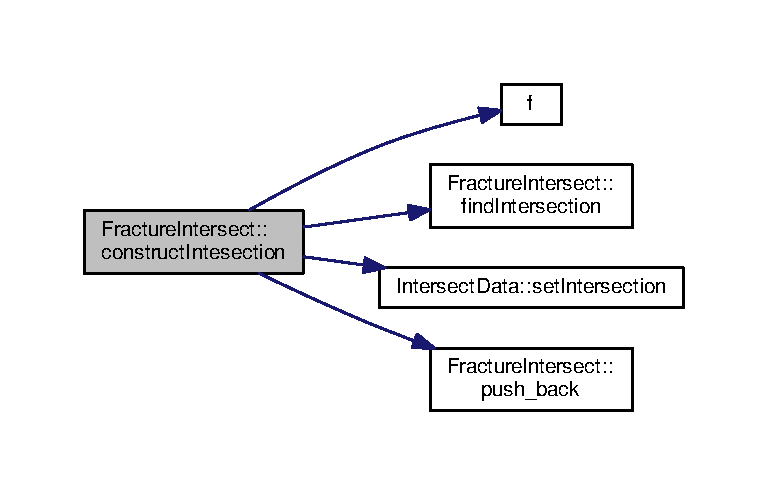
\includegraphics[width=350pt]{classFractureIntersect_a192d02d60bcab84e6ab2765c8167f614_cgraph}
\end{center}
\end{figure}


\hypertarget{classFractureIntersect_a63e99fbb20ef4804cbf99d8f1ab19ac6}{\index{Fracture\-Intersect@{Fracture\-Intersect}!find\-Intersection@{find\-Intersection}}
\index{find\-Intersection@{find\-Intersection}!FractureIntersect@{Fracture\-Intersect}}
\subsubsection[{find\-Intersection}]{\setlength{\rightskip}{0pt plus 5cm}void Fracture\-Intersect\-::find\-Intersection (
\begin{DoxyParamCaption}
\item[{const {\bf Fracture\-Handler\-Ptr\-\_\-\-Type} \&}]{f, }
\item[{const {\bf Fracture\-Ptr\-Container\-\_\-\-Type} \&}]{fractures, }
\item[{{\bf size\-Vector\-\_\-\-Type} \&}]{nodes, }
\item[{{\bf size\-Vector\-\_\-\-Type} \&}]{list\-Of\-Fractures}
\end{DoxyParamCaption}
)}}\label{classFractureIntersect_a63e99fbb20ef4804cbf99d8f1ab19ac6}


Con questa funzione verifico se una data frattura ha intersezione con tutte le altre. 

Quello che ottengo è un vettore di nodi che indica dove la frattura ha intersezione (per ora sarà un nodo solo e, in particolare, sarà il primo o l'ultimo) e la lista degli indice delle fratture con cui ha intersezione 
\begin{DoxyCode}
74 \{
75     size\_type numberFracture = fractures.size();
76     size\_type \hyperlink{namespaceLifeV_a7c0e64679fcd30daa5471b87a57601e9}{ID} = \hyperlink{god__e_8m_a68f477f9b30a6300d5af9b02eac82f35}{f}->getID();
77     size\_type nbDof = \hyperlink{god__e_8m_a68f477f9b30a6300d5af9b02eac82f35}{f}->getData().getSpatialDiscretization ();
78     nodes.clear();
79 
80     \hyperlink{Core_8h_ae3afecb4de4310d8262e9ab20cfb875b}{scalarVectorContainer\_Type} node\_f( 2 );
81     \hyperlink{Core_8h_ae3afecb4de4310d8262e9ab20cfb875b}{scalarVectorContainer\_Type} node\_of( 2 );
82     base\_node t0(1);
83     base\_node t1(1);
84     t0[ 0 ] = 0;
85     t1[ 0 ] = 1;
86 
87     node\_f[ 0 ].push\_back( \hyperlink{god__e_8m_a68f477f9b30a6300d5af9b02eac82f35}{f}->getData ().getA ());
88     node\_f[ 1 ].push\_back( \hyperlink{god__e_8m_a68f477f9b30a6300d5af9b02eac82f35}{f}->getData ().getB ());
89     node\_f[ 0 ].push\_back( \hyperlink{god__e_8m_a68f477f9b30a6300d5af9b02eac82f35}{f}->getLevelSet ()->getData ( )->y\_map( t0 ));
90     node\_f[ 1 ].push\_back( \hyperlink{god__e_8m_a68f477f9b30a6300d5af9b02eac82f35}{f}->getLevelSet ()->getData ( )->y\_map( t1 ));
91 
92     \textcolor{keywordflow}{for} ( size\_type otherFracture = 0; otherFracture < numberFracture; otherFracture++ )
93     \{
94 
95         \textcolor{keywordflow}{if}( otherFracture != ID )
96         \{
97             node\_of[ 0 ].push\_back( fractures[ otherFracture ]->getData ().getA ());
98             node\_of[ 1 ].push\_back( fractures[ otherFracture ]->getData ().getB ());
99             node\_of[ 0 ].push\_back( fractures[ otherFracture ]->getLevelSet ()->getData ( )->y\_map( t0 ));
100             node\_of[ 1 ].push\_back( fractures[ otherFracture ]->getLevelSet ()->getData ( )->y\_map( t1 ));
101 
102             \textcolor{keywordflow}{if}( node\_of[ 0 ][ 0 ] == node\_f[ 0 ][ 0 ] && node\_of[ 0 ][ 1 ] == node\_f[ 0 ][ 1 ] )
103             \{
104                 nodes.push\_back( 0 );
105                 listOfFractures.push\_back( otherFracture );
106             \}
107             \textcolor{keywordflow}{else} \textcolor{keywordflow}{if}( node\_of[ 1 ][ 0 ] == node\_f[ 0 ][ 0 ] && node\_of[ 1 ][ 1 ] == node\_f[ 0 ][ 1 ] )
108             \{
109                 nodes.push\_back( 0 );
110                 listOfFractures.push\_back( otherFracture );
111             \}
112             \textcolor{keywordflow}{else} \textcolor{keywordflow}{if}( node\_of[ 0 ][ 0 ] == node\_f[ 1 ][ 0 ] && node\_of[ 0 ][ 1 ] == node\_f[ 1 ][ 1 ] )
113             \{
114                 nodes.push\_back( nbDof-1 );
115                 listOfFractures.push\_back( otherFracture );
116             \}
117             \textcolor{keywordflow}{else} \textcolor{keywordflow}{if}( node\_of[ 1 ][ 0 ] == node\_f[ 1 ][ 0 ] && node\_of[ 1 ][ 1 ] == node\_f[ 1 ][ 1 ] )
118             \{
119                 nodes.push\_back( nbDof-1 );
120                 listOfFractures.push\_back( otherFracture );
121             \}
122 
123 
124 
125         \}
126 
127     \}
128 
129 \}\textcolor{comment}{// findIntersection}
\end{DoxyCode}


Questo è il grafo dei chiamanti di questa funzione\-:
\nopagebreak
\begin{figure}[H]
\begin{center}
\leavevmode
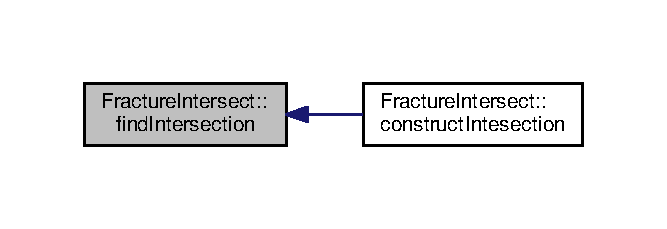
\includegraphics[width=320pt]{classFractureIntersect_a63e99fbb20ef4804cbf99d8f1ab19ac6_icgraph}
\end{center}
\end{figure}


\hypertarget{classFractureIntersect_a18ff664767b7e8ffa876b80a6100e74d}{\index{Fracture\-Intersect@{Fracture\-Intersect}!get\-Bifurcation\-Intersections@{get\-Bifurcation\-Intersections}}
\index{get\-Bifurcation\-Intersections@{get\-Bifurcation\-Intersections}!FractureIntersect@{Fracture\-Intersect}}
\subsubsection[{get\-Bifurcation\-Intersections}]{\setlength{\rightskip}{0pt plus 5cm}{\bf Intersect\-Data\-Container\-\_\-\-Type} Fracture\-Intersect\-::get\-Bifurcation\-Intersections (
\begin{DoxyParamCaption}
{}
\end{DoxyParamCaption}
) const}}\label{classFractureIntersect_a18ff664767b7e8ffa876b80a6100e74d}


Funzione che restituisce tutte le intersezioni di tipo \char`\"{} Bifurcation \char`\"{}. 

\begin{DoxyReturn}{Restituisce}
Intersect\-Data\-Container\-\_\-\-Type\-: restituisce il vettore di tutte le intersezioni del tipo \char`\"{} Bifurcation \char`\"{} 
\end{DoxyReturn}

\begin{DoxyCode}
180 \{
181     \hyperlink{IntersectData_8h_a822ec3b760dfb603e1cf0bfe3ad5636a}{IntersectDataContainer\_Type} tmp;
182 
183     size\_type Num\_Bifu = \hyperlink{classFractureIntersect_afba7c92096a4b92a27fcb4f1158c7279}{getNumberBifurcation}();
184 
185     \textcolor{keywordflow}{if}( Num\_Bifu !=0 )
186     \{
187         \textcolor{keywordflow}{for} ( size\_type \hyperlink{god__e_8m_a8604be5925f4266ab5ccc69675329c80}{i} = 0; \hyperlink{god__e_8m_a8604be5925f4266ab5ccc69675329c80}{i}< M\_intersections.size(); \hyperlink{god__e_8m_a8604be5925f4266ab5ccc69675329c80}{i}++ )
188         \{
189             \textcolor{keywordflow}{if} ( M\_intersections[ \hyperlink{god__e_8m_a8604be5925f4266ab5ccc69675329c80}{i} ].getNumFractures () == 3 )
190             \{
191                 tmp.push\_back( M\_intersections[ \hyperlink{god__e_8m_a8604be5925f4266ab5ccc69675329c80}{i} ] );
192             \}
193         \}
194     \}
195 
196     \textcolor{keywordflow}{return} tmp;
197 
198 \} \textcolor{comment}{// getBifurcationIntersections}
\end{DoxyCode}


Questo è il grafo delle chiamate per questa funzione\-:
\nopagebreak
\begin{figure}[H]
\begin{center}
\leavevmode
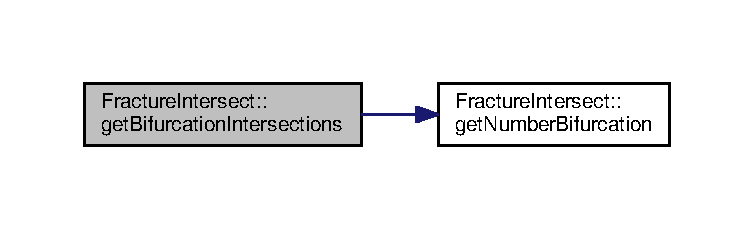
\includegraphics[width=350pt]{classFractureIntersect_a18ff664767b7e8ffa876b80a6100e74d_cgraph}
\end{center}
\end{figure}


\hypertarget{classFractureIntersect_a248df8f326f844e34d807234efdfd693}{\index{Fracture\-Intersect@{Fracture\-Intersect}!get\-Cross\-Intersections@{get\-Cross\-Intersections}}
\index{get\-Cross\-Intersections@{get\-Cross\-Intersections}!FractureIntersect@{Fracture\-Intersect}}
\subsubsection[{get\-Cross\-Intersections}]{\setlength{\rightskip}{0pt plus 5cm}{\bf Intersect\-Data\-Container\-\_\-\-Type} Fracture\-Intersect\-::get\-Cross\-Intersections (
\begin{DoxyParamCaption}
{}
\end{DoxyParamCaption}
) const}}\label{classFractureIntersect_a248df8f326f844e34d807234efdfd693}


Funzione che restituisce tutte le intersezioni di tipo \char`\"{} Cross \char`\"{}. 

\begin{DoxyReturn}{Restituisce}
Intersect\-Data\-Container\-\_\-\-Type\-: restituisce il vettore di tutte le intersezioni del tipo \char`\"{} Cross \char`\"{} 
\end{DoxyReturn}

\begin{DoxyCode}
159 \{
160     \hyperlink{IntersectData_8h_a822ec3b760dfb603e1cf0bfe3ad5636a}{IntersectDataContainer\_Type} tmp;
161     size\_type Num\_Cross = \hyperlink{classFractureIntersect_a8d9f707319b9b83744b6e03f19003734}{getNumberCross}();
162 
163     \textcolor{keywordflow}{if}( Num\_Cross !=0 )
164     \{
165         \textcolor{keywordflow}{for} ( size\_type \hyperlink{god__e_8m_a8604be5925f4266ab5ccc69675329c80}{i} = 0; \hyperlink{god__e_8m_a8604be5925f4266ab5ccc69675329c80}{i}< M\_intersections.size(); \hyperlink{god__e_8m_a8604be5925f4266ab5ccc69675329c80}{i}++ )
166         \{
167             \textcolor{keywordflow}{if} ( M\_intersections[ \hyperlink{god__e_8m_a8604be5925f4266ab5ccc69675329c80}{i} ].getNumFractures () == 2 )
168             \{
169                 tmp.push\_back( M\_intersections[ \hyperlink{god__e_8m_a8604be5925f4266ab5ccc69675329c80}{i} ] );
170             \}
171         \}
172     \}
173 
174     \textcolor{keywordflow}{return} tmp;
175 
176 \} \textcolor{comment}{// getCrossIntersections}
\end{DoxyCode}


Questo è il grafo delle chiamate per questa funzione\-:
\nopagebreak
\begin{figure}[H]
\begin{center}
\leavevmode
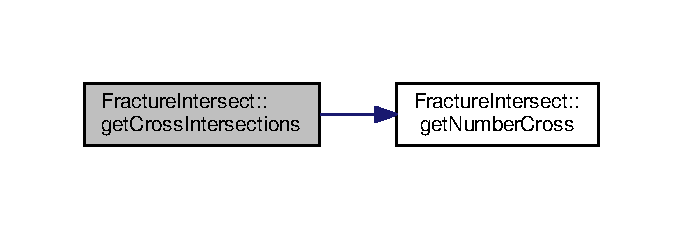
\includegraphics[width=328pt]{classFractureIntersect_a248df8f326f844e34d807234efdfd693_cgraph}
\end{center}
\end{figure}


\hypertarget{classFractureIntersect_afba7c92096a4b92a27fcb4f1158c7279}{\index{Fracture\-Intersect@{Fracture\-Intersect}!get\-Number\-Bifurcation@{get\-Number\-Bifurcation}}
\index{get\-Number\-Bifurcation@{get\-Number\-Bifurcation}!FractureIntersect@{Fracture\-Intersect}}
\subsubsection[{get\-Number\-Bifurcation}]{\setlength{\rightskip}{0pt plus 5cm}size\-\_\-type Fracture\-Intersect\-::get\-Number\-Bifurcation (
\begin{DoxyParamCaption}
{}
\end{DoxyParamCaption}
) const}}\label{classFractureIntersect_afba7c92096a4b92a27fcb4f1158c7279}

\begin{DoxyCode}
218 \{
219     size\_type count = 0;
220 
221     \textcolor{keywordflow}{for} ( size\_type \hyperlink{god__e_8m_a8604be5925f4266ab5ccc69675329c80}{i} = 0; \hyperlink{god__e_8m_a8604be5925f4266ab5ccc69675329c80}{i} < M\_intersections.size (); \hyperlink{god__e_8m_a8604be5925f4266ab5ccc69675329c80}{i}++ )
222     \{
223         \textcolor{keywordflow}{if} ( M\_intersections[ \hyperlink{god__e_8m_a8604be5925f4266ab5ccc69675329c80}{i} ].getFractures().size() == 3 )
224         \{
225             count ++;
226         \}
227     \}
228 
229     \textcolor{keywordflow}{return} count;
230 \}\textcolor{comment}{// getNumberBifurcation}
\end{DoxyCode}


Questo è il grafo dei chiamanti di questa funzione\-:
\nopagebreak
\begin{figure}[H]
\begin{center}
\leavevmode
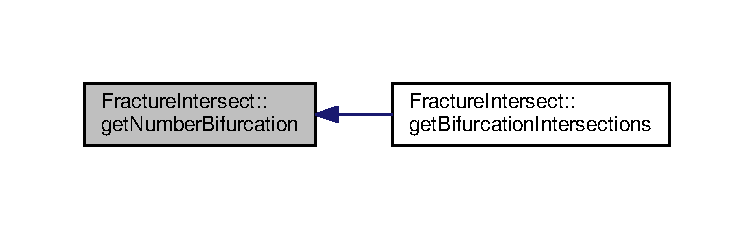
\includegraphics[width=350pt]{classFractureIntersect_afba7c92096a4b92a27fcb4f1158c7279_icgraph}
\end{center}
\end{figure}


\hypertarget{classFractureIntersect_a8d9f707319b9b83744b6e03f19003734}{\index{Fracture\-Intersect@{Fracture\-Intersect}!get\-Number\-Cross@{get\-Number\-Cross}}
\index{get\-Number\-Cross@{get\-Number\-Cross}!FractureIntersect@{Fracture\-Intersect}}
\subsubsection[{get\-Number\-Cross}]{\setlength{\rightskip}{0pt plus 5cm}size\-\_\-type Fracture\-Intersect\-::get\-Number\-Cross (
\begin{DoxyParamCaption}
{}
\end{DoxyParamCaption}
) const}}\label{classFractureIntersect_a8d9f707319b9b83744b6e03f19003734}

\begin{DoxyCode}
203 \{
204     size\_type count = 0;
205 
206     \textcolor{keywordflow}{for} ( size\_type \hyperlink{god__e_8m_a8604be5925f4266ab5ccc69675329c80}{i} = 0; \hyperlink{god__e_8m_a8604be5925f4266ab5ccc69675329c80}{i} < M\_intersections.size (); \hyperlink{god__e_8m_a8604be5925f4266ab5ccc69675329c80}{i}++ )
207     \{
208         \textcolor{keywordflow}{if} ( M\_intersections[ \hyperlink{god__e_8m_a8604be5925f4266ab5ccc69675329c80}{i} ].getFractures().size() == 2 )
209         \{
210             count ++;
211         \}
212     \}
213 
214     \textcolor{keywordflow}{return} count;
215 \}\textcolor{comment}{// getNumberCross}
\end{DoxyCode}


Questo è il grafo dei chiamanti di questa funzione\-:
\nopagebreak
\begin{figure}[H]
\begin{center}
\leavevmode
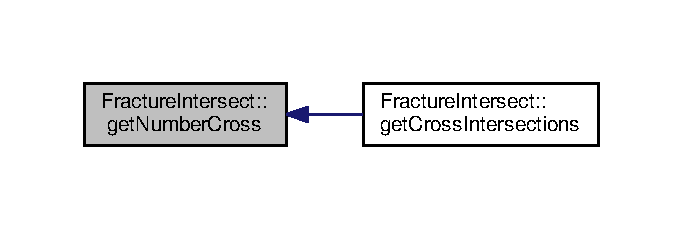
\includegraphics[width=328pt]{classFractureIntersect_a8d9f707319b9b83744b6e03f19003734_icgraph}
\end{center}
\end{figure}


\hypertarget{classFractureIntersect_a01bc187a846208a47a13daeeb94b13f5}{\index{Fracture\-Intersect@{Fracture\-Intersect}!push\-\_\-back@{push\-\_\-back}}
\index{push\-\_\-back@{push\-\_\-back}!FractureIntersect@{Fracture\-Intersect}}
\subsubsection[{push\-\_\-back}]{\setlength{\rightskip}{0pt plus 5cm}void Fracture\-Intersect\-::push\-\_\-back (
\begin{DoxyParamCaption}
\item[{const {\bf Intersect\-Data} \&}]{intersection}
\end{DoxyParamCaption}
)}}\label{classFractureIntersect_a01bc187a846208a47a13daeeb94b13f5}


Dopo aver costruito una nuova intersezione, prima di inserirla nel vettore delle intersezioni, verifico che non vi sia già. 

In tal caso non inserisco le fratture coinvolte, ma solo gli indici dei nodi corrispondenti non ancora inseriti 
\begin{DoxyCode}
133 \{
134     \textcolor{keywordflow}{if} ( M\_intersections.size() == 0 )
135     \{
136         M\_intersections.push\_back( intersection );
137     \}
138     \textcolor{keywordflow}{else}
139     \{
140         \textcolor{keywordflow}{for} ( size\_type \hyperlink{god__e_8m_a8604be5925f4266ab5ccc69675329c80}{i} = 0; \hyperlink{god__e_8m_a8604be5925f4266ab5ccc69675329c80}{i} < M\_intersections.size(); \hyperlink{god__e_8m_a8604be5925f4266ab5ccc69675329c80}{i}++ )
141         \{
142             \textcolor{keywordflow}{if}( M\_intersections[ \hyperlink{god__e_8m_a8604be5925f4266ab5ccc69675329c80}{i} ].isEqual( intersection ))
143             \{
144                 M\_intersections[ \hyperlink{god__e_8m_a8604be5925f4266ab5ccc69675329c80}{i} ].updateNodes( intersection );
145             \}
146             \textcolor{keywordflow}{else}
147             \{
148                 M\_intersections.push\_back( intersection );
149             \}
150         \}
151     \}
152 
153     \textcolor{keywordflow}{return};
154 \}\textcolor{comment}{// push\_back}
\end{DoxyCode}


Questo è il grafo dei chiamanti di questa funzione\-:
\nopagebreak
\begin{figure}[H]
\begin{center}
\leavevmode
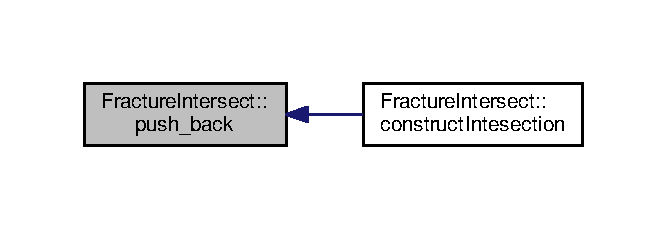
\includegraphics[width=320pt]{classFractureIntersect_a01bc187a846208a47a13daeeb94b13f5_icgraph}
\end{center}
\end{figure}




La documentazione per questa classe è stata generata a partire dai seguenti file\-:\begin{DoxyCompactItemize}
\item 
include/\hyperlink{FractureIntersect_8h}{Fracture\-Intersect.\-h}\item 
src/\hyperlink{FractureIntersect_8cc}{Fracture\-Intersect.\-cc}\end{DoxyCompactItemize}

\hypertarget{classFracturesSet}{\section{Riferimenti per la classe Fractures\-Set}
\label{classFracturesSet}\index{Fractures\-Set@{Fractures\-Set}}
}


{\ttfamily \#include $<$Fractures\-Set.\-h$>$}

\subsection*{Membri pubblici}
\begin{DoxyCompactItemize}
\item 
\hyperlink{classFracturesSet_a01682537586e273be19fd789c99cfa87}{Fractures\-Set} ()
\item 
void \hyperlink{classFracturesSet_afdaec960c5e2bca4e999e692675895d7}{init} (const Get\-Pot \&data\-File, const std\-::string \&section, const size\-\_\-type \&num\-Fractures, const \hyperlink{Exporter_8h_ac9d7f94fea8b91459a536bfaa2f3910c}{Exporter\-Ptr\-\_\-\-Type} \&exporter)
\item 
const \hyperlink{FractureHandler_8h_af23fb7a30aaff864bd42587af4f1e78a}{Fracture\-Handler\-Ptr\-\_\-\-Type} \& \hyperlink{classFracturesSet_afa7100ac44d32e51e193380bf6d9d5f9}{get\-Fracture} (const size\-\_\-type \&\hyperlink{god__e_8m_a8ea372f7ee3c01d11fc4b4d13b8e6a75}{f}) const 
\item 
size\-\_\-type \hyperlink{classFracturesSet_ad0d608408d6b65c83c2eb013d4daacdf}{get\-Number\-Fractures} () const 
\item 
const \hyperlink{FractureIntersect_8h_a5486417d11465ffafe3034ce22c1c85b}{Fracture\-Intersect\-Ptr\-\_\-\-Type} \& \hyperlink{classFracturesSet_ae1d7e53adc5d8acaad0a37dd227aee03}{get\-Intersections} () const 
\end{DoxyCompactItemize}


\subsection{Documentazione dei costruttori e dei distruttori}
\hypertarget{classFracturesSet_a01682537586e273be19fd789c99cfa87}{\index{Fractures\-Set@{Fractures\-Set}!Fractures\-Set@{Fractures\-Set}}
\index{Fractures\-Set@{Fractures\-Set}!FracturesSet@{Fractures\-Set}}
\subsubsection[{Fractures\-Set}]{\setlength{\rightskip}{0pt plus 5cm}Fractures\-Set\-::\-Fractures\-Set (
\begin{DoxyParamCaption}
{}
\end{DoxyParamCaption}
)}}\label{classFracturesSet_a01682537586e273be19fd789c99cfa87}

\begin{DoxyCode}
9                           :
10                 M\_intersections(\textcolor{keyword}{new} \hyperlink{classFractureIntersect}{FractureIntersect\_Type})
11 \{\}\textcolor{comment}{// costruttore nullo}
\end{DoxyCode}


\subsection{Documentazione delle funzioni membro}
\hypertarget{classFracturesSet_afa7100ac44d32e51e193380bf6d9d5f9}{\index{Fractures\-Set@{Fractures\-Set}!get\-Fracture@{get\-Fracture}}
\index{get\-Fracture@{get\-Fracture}!FracturesSet@{Fractures\-Set}}
\subsubsection[{get\-Fracture}]{\setlength{\rightskip}{0pt plus 5cm}const {\bf Fracture\-Handler\-Ptr\-\_\-\-Type}\& Fractures\-Set\-::get\-Fracture (
\begin{DoxyParamCaption}
\item[{const size\-\_\-type \&}]{f}
\end{DoxyParamCaption}
) const\hspace{0.3cm}{\ttfamily [inline]}}}\label{classFracturesSet_afa7100ac44d32e51e193380bf6d9d5f9}

\begin{DoxyCode}
33     \{
34             \textcolor{keywordflow}{return} M\_fractures[\hyperlink{god__e_8m_a68f477f9b30a6300d5af9b02eac82f35}{f}];
35     \}
\end{DoxyCode}


Questo è il grafo delle chiamate per questa funzione\-:
\nopagebreak
\begin{figure}[H]
\begin{center}
\leavevmode
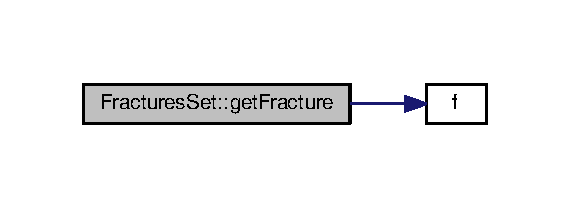
\includegraphics[width=274pt]{classFracturesSet_afa7100ac44d32e51e193380bf6d9d5f9_cgraph}
\end{center}
\end{figure}


\hypertarget{classFracturesSet_ae1d7e53adc5d8acaad0a37dd227aee03}{\index{Fractures\-Set@{Fractures\-Set}!get\-Intersections@{get\-Intersections}}
\index{get\-Intersections@{get\-Intersections}!FracturesSet@{Fractures\-Set}}
\subsubsection[{get\-Intersections}]{\setlength{\rightskip}{0pt plus 5cm}const {\bf Fracture\-Intersect\-Ptr\-\_\-\-Type}\& Fractures\-Set\-::get\-Intersections (
\begin{DoxyParamCaption}
{}
\end{DoxyParamCaption}
) const\hspace{0.3cm}{\ttfamily [inline]}}}\label{classFracturesSet_ae1d7e53adc5d8acaad0a37dd227aee03}

\begin{DoxyCode}
43     \{
44         \textcolor{keywordflow}{return} M\_intersections;
45     \}
\end{DoxyCode}
\hypertarget{classFracturesSet_ad0d608408d6b65c83c2eb013d4daacdf}{\index{Fractures\-Set@{Fractures\-Set}!get\-Number\-Fractures@{get\-Number\-Fractures}}
\index{get\-Number\-Fractures@{get\-Number\-Fractures}!FracturesSet@{Fractures\-Set}}
\subsubsection[{get\-Number\-Fractures}]{\setlength{\rightskip}{0pt plus 5cm}size\-\_\-type Fractures\-Set\-::get\-Number\-Fractures (
\begin{DoxyParamCaption}
{}
\end{DoxyParamCaption}
) const\hspace{0.3cm}{\ttfamily [inline]}}}\label{classFracturesSet_ad0d608408d6b65c83c2eb013d4daacdf}

\begin{DoxyCode}
38     \{
39         \textcolor{keywordflow}{return} M\_fractures.size();
40     \}
\end{DoxyCode}
\hypertarget{classFracturesSet_afdaec960c5e2bca4e999e692675895d7}{\index{Fractures\-Set@{Fractures\-Set}!init@{init}}
\index{init@{init}!FracturesSet@{Fractures\-Set}}
\subsubsection[{init}]{\setlength{\rightskip}{0pt plus 5cm}void Fractures\-Set\-::init (
\begin{DoxyParamCaption}
\item[{const Get\-Pot \&}]{data\-File, }
\item[{const std\-::string \&}]{section, }
\item[{const size\-\_\-type \&}]{num\-Fractures, }
\item[{const {\bf Exporter\-Ptr\-\_\-\-Type} \&}]{exporter}
\end{DoxyParamCaption}
)}}\label{classFracturesSet_afdaec960c5e2bca4e999e692675895d7}

\begin{DoxyCode}
15 \{
16     M\_fractures.resize( numFractures );
17 
18     std::ostringstream sectionFracture;
19 
20     \textcolor{keywordflow}{for} ( size\_type \hyperlink{god__e_8m_a68f477f9b30a6300d5af9b02eac82f35}{f} = 0; \hyperlink{god__e_8m_a68f477f9b30a6300d5af9b02eac82f35}{f} < numFractures; \hyperlink{god__e_8m_a68f477f9b30a6300d5af9b02eac82f35}{f}++ )
21     \{
22         sectionFracture << section << \textcolor{stringliteral}{"fractureData"} << \hyperlink{god__e_8m_a68f477f9b30a6300d5af9b02eac82f35}{f} << \textcolor{stringliteral}{"/"};
23 
24         M\_fractures [ \hyperlink{god__e_8m_a68f477f9b30a6300d5af9b02eac82f35}{f} ].reset ( \textcolor{keyword}{new} \hyperlink{classFractureHandler}{FractureHandler\_Type} ( dataFile, f, exporter, 
      sectionFracture.str() ));
25 
26         M\_fractures [ \hyperlink{god__e_8m_a68f477f9b30a6300d5af9b02eac82f35}{f} ]->init();
27 
28         M\_fractures [ \hyperlink{god__e_8m_a68f477f9b30a6300d5af9b02eac82f35}{f} ]->numFractures ( numFractures );
29 
30         sectionFracture.str(\textcolor{stringliteral}{""});
31     \}
32 
33     std::cout << \textcolor{stringliteral}{"costruisco l'intersezione "} << std::endl;
34     \textcolor{comment}{// costruisco l'intersezione}
35     M\_intersections->constructIntesection ( M\_fractures );
36 
37     \textcolor{keywordflow}{return};
38 \}\textcolor{comment}{// init}
\end{DoxyCode}


Questo è il grafo delle chiamate per questa funzione\-:
\nopagebreak
\begin{figure}[H]
\begin{center}
\leavevmode
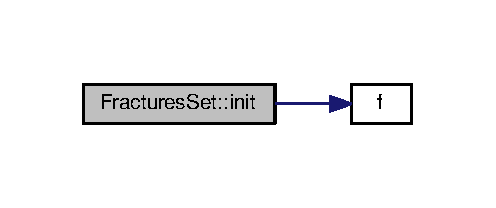
\includegraphics[width=238pt]{classFracturesSet_afdaec960c5e2bca4e999e692675895d7_cgraph}
\end{center}
\end{figure}




La documentazione per questa classe è stata generata a partire dai seguenti file\-:\begin{DoxyCompactItemize}
\item 
include/\hyperlink{FracturesSet_8h}{Fractures\-Set.\-h}\item 
src/\hyperlink{FracturesSet_8cc}{Fractures\-Set.\-cc}\end{DoxyCompactItemize}

\hypertarget{classIntersectData}{\section{Riferimenti per la classe Intersect\-Data}
\label{classIntersectData}\index{Intersect\-Data@{Intersect\-Data}}
}


{\ttfamily \#include $<$Intersect\-Data.\-h$>$}

\subsection*{Membri pubblici}
\begin{DoxyCompactItemize}
\item 
\hyperlink{classIntersectData_ac86ac869672ccd193327ce246e7969d6}{Intersect\-Data} ()
\item 
\hyperlink{classIntersectData_a731a27ad828cdc8146679a292cbd4582}{Intersect\-Data} (const \hyperlink{classIntersectData}{Intersect\-Data} \&in)
\item 
void \hyperlink{classIntersectData_a4dbe681fa68704c9e2bf3f8e290b55f7}{set\-Intersection} (const \hyperlink{Core_8h_a83c51913d041a5001e8683434c09857f}{size\-Vector\-\_\-\-Type} \&nodes, const \hyperlink{FractureHandler_8h_a2f0b57e18ecf89912d7de0c87158009e}{Fracture\-Ptr\-Container\-\_\-\-Type} \&fractures)
\begin{DoxyCompactList}\small\item\em Funzione che definisce l'intersezione\-: definisce le fratture coinvolte e assegna al vettore dei nodi la dimensione corretta, ossia pari al numero di fratture. \end{DoxyCompactList}\item 
bool \hyperlink{classIntersectData_acbb362d913af755b71fa801e3a507a63}{is\-Equal} (const \hyperlink{classIntersectData}{Intersect\-Data} \&intersection)
\begin{DoxyCompactList}\small\item\em Funzione che verifica se due intersezioni sono uguali a meno dei nodi, ossia se le fratture coinvolte sono le stesse. \end{DoxyCompactList}\item 
void \hyperlink{classIntersectData_a6bcd52066286893ea1f7c36ea841da82}{update\-Nodes} (const \hyperlink{classIntersectData}{Intersect\-Data} \&intersection)
\begin{DoxyCompactList}\small\item\em Funzione che aggiunge uno degli indici dei nodi di intersezione mancanti. \end{DoxyCompactList}\item 
const \hyperlink{FractureHandler_8h_a2f0b57e18ecf89912d7de0c87158009e}{Fracture\-Ptr\-Container\-\_\-\-Type} \& \hyperlink{classIntersectData_a1c43bd327ed8dedaa89870f60cdb4606}{get\-Fractures} () const 
\item 
const \hyperlink{FractureHandler_8h_af23fb7a30aaff864bd42587af4f1e78a}{Fracture\-Handler\-Ptr\-\_\-\-Type} \& \hyperlink{classIntersectData_afef7730d6a494464350ebce088e488ee}{get\-Fracture} (const size\-\_\-type \&\hyperlink{god__e_8m_a8ea372f7ee3c01d11fc4b4d13b8e6a75}{f}) const 
\item 
size\-\_\-type \hyperlink{classIntersectData_a25def82d58f9508d33ab1a43b2b03ceb}{get\-Num\-Fractures} () const 
\item 
\hyperlink{Core_8h_a83c51913d041a5001e8683434c09857f}{size\-Vector\-\_\-\-Type} \hyperlink{classIntersectData_aed138ba9b2e3e33d55999db110871406}{get\-Intersection\-Point} () const 
\end{DoxyCompactItemize}


\subsection{Documentazione dei costruttori e dei distruttori}
\hypertarget{classIntersectData_ac86ac869672ccd193327ce246e7969d6}{\index{Intersect\-Data@{Intersect\-Data}!Intersect\-Data@{Intersect\-Data}}
\index{Intersect\-Data@{Intersect\-Data}!IntersectData@{Intersect\-Data}}
\subsubsection[{Intersect\-Data}]{\setlength{\rightskip}{0pt plus 5cm}Intersect\-Data\-::\-Intersect\-Data (
\begin{DoxyParamCaption}
{}
\end{DoxyParamCaption}
)\hspace{0.3cm}{\ttfamily [inline]}}}\label{classIntersectData_ac86ac869672ccd193327ce246e7969d6}

\begin{DoxyCode}
29     \{\};
\end{DoxyCode}
\hypertarget{classIntersectData_a731a27ad828cdc8146679a292cbd4582}{\index{Intersect\-Data@{Intersect\-Data}!Intersect\-Data@{Intersect\-Data}}
\index{Intersect\-Data@{Intersect\-Data}!IntersectData@{Intersect\-Data}}
\subsubsection[{Intersect\-Data}]{\setlength{\rightskip}{0pt plus 5cm}Intersect\-Data\-::\-Intersect\-Data (
\begin{DoxyParamCaption}
\item[{const {\bf Intersect\-Data} \&}]{in}
\end{DoxyParamCaption}
)\hspace{0.3cm}{\ttfamily [inline]}}}\label{classIntersectData_a731a27ad828cdc8146679a292cbd4582}

\begin{DoxyCode}
33     \{
34         copy ( in );
35     \} \textcolor{comment}{// costruttore di copia}
\end{DoxyCode}


\subsection{Documentazione delle funzioni membro}
\hypertarget{classIntersectData_afef7730d6a494464350ebce088e488ee}{\index{Intersect\-Data@{Intersect\-Data}!get\-Fracture@{get\-Fracture}}
\index{get\-Fracture@{get\-Fracture}!IntersectData@{Intersect\-Data}}
\subsubsection[{get\-Fracture}]{\setlength{\rightskip}{0pt plus 5cm}const {\bf Fracture\-Handler\-Ptr\-\_\-\-Type}\& Intersect\-Data\-::get\-Fracture (
\begin{DoxyParamCaption}
\item[{const size\-\_\-type \&}]{f}
\end{DoxyParamCaption}
) const\hspace{0.3cm}{\ttfamily [inline]}}}\label{classIntersectData_afef7730d6a494464350ebce088e488ee}

\begin{DoxyCode}
63     \{
64         \textcolor{keywordflow}{return} M\_fractures [ \hyperlink{god__e_8m_a68f477f9b30a6300d5af9b02eac82f35}{f} ];
65     \} \textcolor{comment}{// getFracture}
\end{DoxyCode}


Questo è il grafo delle chiamate per questa funzione\-:
\nopagebreak
\begin{figure}[H]
\begin{center}
\leavevmode
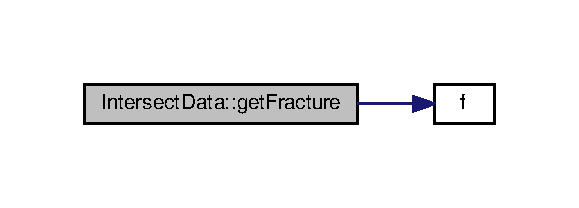
\includegraphics[width=278pt]{classIntersectData_afef7730d6a494464350ebce088e488ee_cgraph}
\end{center}
\end{figure}




Questo è il grafo dei chiamanti di questa funzione\-:
\nopagebreak
\begin{figure}[H]
\begin{center}
\leavevmode
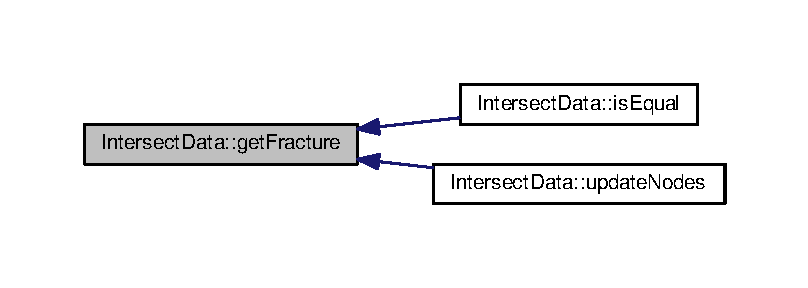
\includegraphics[width=350pt]{classIntersectData_afef7730d6a494464350ebce088e488ee_icgraph}
\end{center}
\end{figure}


\hypertarget{classIntersectData_a1c43bd327ed8dedaa89870f60cdb4606}{\index{Intersect\-Data@{Intersect\-Data}!get\-Fractures@{get\-Fractures}}
\index{get\-Fractures@{get\-Fractures}!IntersectData@{Intersect\-Data}}
\subsubsection[{get\-Fractures}]{\setlength{\rightskip}{0pt plus 5cm}const {\bf Fracture\-Ptr\-Container\-\_\-\-Type}\& Intersect\-Data\-::get\-Fractures (
\begin{DoxyParamCaption}
{}
\end{DoxyParamCaption}
) const\hspace{0.3cm}{\ttfamily [inline]}}}\label{classIntersectData_a1c43bd327ed8dedaa89870f60cdb4606}

\begin{DoxyCode}
58     \{
59         \textcolor{keywordflow}{return} M\_fractures;
60     \} \textcolor{comment}{// getFractures}
\end{DoxyCode}


Questo è il grafo dei chiamanti di questa funzione\-:
\nopagebreak
\begin{figure}[H]
\begin{center}
\leavevmode
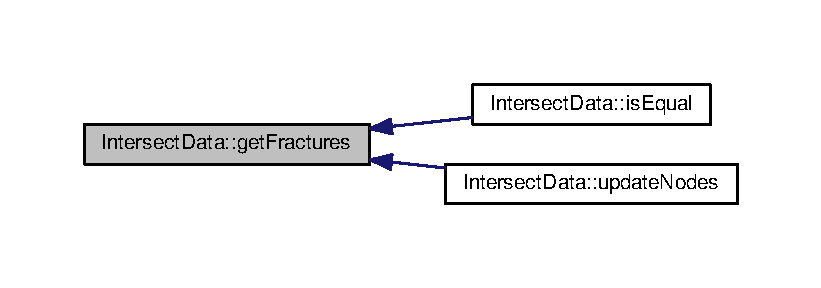
\includegraphics[width=350pt]{classIntersectData_a1c43bd327ed8dedaa89870f60cdb4606_icgraph}
\end{center}
\end{figure}


\hypertarget{classIntersectData_aed138ba9b2e3e33d55999db110871406}{\index{Intersect\-Data@{Intersect\-Data}!get\-Intersection\-Point@{get\-Intersection\-Point}}
\index{get\-Intersection\-Point@{get\-Intersection\-Point}!IntersectData@{Intersect\-Data}}
\subsubsection[{get\-Intersection\-Point}]{\setlength{\rightskip}{0pt plus 5cm}{\bf size\-Vector\-\_\-\-Type} Intersect\-Data\-::get\-Intersection\-Point (
\begin{DoxyParamCaption}
{}
\end{DoxyParamCaption}
) const\hspace{0.3cm}{\ttfamily [inline]}}}\label{classIntersectData_aed138ba9b2e3e33d55999db110871406}

\begin{DoxyCode}
74     \{
75         \textcolor{keywordflow}{return} M\_intersectionPoint;
76     \}
\end{DoxyCode}


Questo è il grafo dei chiamanti di questa funzione\-:
\nopagebreak
\begin{figure}[H]
\begin{center}
\leavevmode
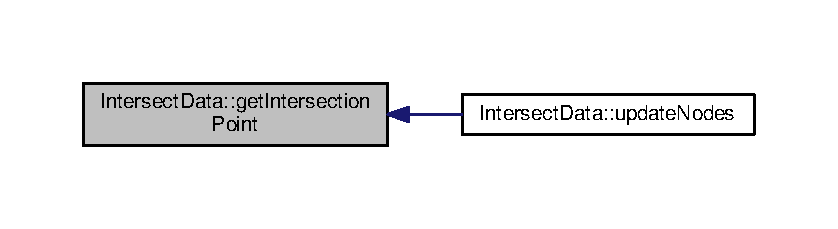
\includegraphics[width=350pt]{classIntersectData_aed138ba9b2e3e33d55999db110871406_icgraph}
\end{center}
\end{figure}


\hypertarget{classIntersectData_a25def82d58f9508d33ab1a43b2b03ceb}{\index{Intersect\-Data@{Intersect\-Data}!get\-Num\-Fractures@{get\-Num\-Fractures}}
\index{get\-Num\-Fractures@{get\-Num\-Fractures}!IntersectData@{Intersect\-Data}}
\subsubsection[{get\-Num\-Fractures}]{\setlength{\rightskip}{0pt plus 5cm}size\-\_\-type Intersect\-Data\-::get\-Num\-Fractures (
\begin{DoxyParamCaption}
{}
\end{DoxyParamCaption}
) const\hspace{0.3cm}{\ttfamily [inline]}}}\label{classIntersectData_a25def82d58f9508d33ab1a43b2b03ceb}

\begin{DoxyCode}
69     \{
70         \textcolor{keywordflow}{return} M\_fractures.size();
71     \} \textcolor{comment}{// getNumFractures}
\end{DoxyCode}
\hypertarget{classIntersectData_acbb362d913af755b71fa801e3a507a63}{\index{Intersect\-Data@{Intersect\-Data}!is\-Equal@{is\-Equal}}
\index{is\-Equal@{is\-Equal}!IntersectData@{Intersect\-Data}}
\subsubsection[{is\-Equal}]{\setlength{\rightskip}{0pt plus 5cm}bool Intersect\-Data\-::is\-Equal (
\begin{DoxyParamCaption}
\item[{const {\bf Intersect\-Data} \&}]{intersection}
\end{DoxyParamCaption}
)}}\label{classIntersectData_acbb362d913af755b71fa801e3a507a63}


Funzione che verifica se due intersezioni sono uguali a meno dei nodi, ossia se le fratture coinvolte sono le stesse. 


\begin{DoxyCode}
43 \{
44     size\_type count = 0;
45 
46     \textcolor{keywordflow}{if} ( M\_fractures.size() != intersection.\hyperlink{classIntersectData_a1c43bd327ed8dedaa89870f60cdb4606}{getFractures} ().size() )
47     \{
48         \textcolor{keywordflow}{return} \textcolor{keyword}{false};
49     \}
50     \textcolor{keywordflow}{else}
51     \{
52         \textcolor{keywordflow}{for} ( size\_type \hyperlink{god__e_8m_a8604be5925f4266ab5ccc69675329c80}{i} = 0; \hyperlink{god__e_8m_a8604be5925f4266ab5ccc69675329c80}{i} < M\_fractures.size(); \hyperlink{god__e_8m_a8604be5925f4266ab5ccc69675329c80}{i}++ )
53         \{
54             \textcolor{keywordflow}{for} ( size\_type j = 0; j < intersection.\hyperlink{classIntersectData_a1c43bd327ed8dedaa89870f60cdb4606}{getFractures} ().size(); j++ )
55             \{
56                 \textcolor{keywordflow}{if} ( M\_fractures[ \hyperlink{god__e_8m_a8604be5925f4266ab5ccc69675329c80}{i} ]->getID() == intersection.\hyperlink{classIntersectData_afef7730d6a494464350ebce088e488ee}{getFracture} ( j )->getID () )
57                 \{
58                     count ++;
59                 \}
60             \}
61         \}
62 
63         \textcolor{keywordflow}{return} ( count == M\_fractures.size() );
64     \}
65 \}\textcolor{comment}{// isEqual}
\end{DoxyCode}


Questo è il grafo delle chiamate per questa funzione\-:
\nopagebreak
\begin{figure}[H]
\begin{center}
\leavevmode
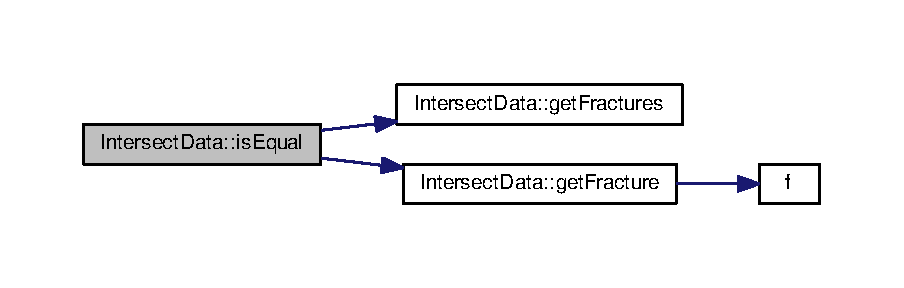
\includegraphics[width=350pt]{classIntersectData_acbb362d913af755b71fa801e3a507a63_cgraph}
\end{center}
\end{figure}


\hypertarget{classIntersectData_a4dbe681fa68704c9e2bf3f8e290b55f7}{\index{Intersect\-Data@{Intersect\-Data}!set\-Intersection@{set\-Intersection}}
\index{set\-Intersection@{set\-Intersection}!IntersectData@{Intersect\-Data}}
\subsubsection[{set\-Intersection}]{\setlength{\rightskip}{0pt plus 5cm}void Intersect\-Data\-::set\-Intersection (
\begin{DoxyParamCaption}
\item[{const {\bf size\-Vector\-\_\-\-Type} \&}]{nodes, }
\item[{const {\bf Fracture\-Ptr\-Container\-\_\-\-Type} \&}]{fractures}
\end{DoxyParamCaption}
)}}\label{classIntersectData_a4dbe681fa68704c9e2bf3f8e290b55f7}


Funzione che definisce l'intersezione\-: definisce le fratture coinvolte e assegna al vettore dei nodi la dimensione corretta, ossia pari al numero di fratture. 

Questo perchè per ogni frattura coinvolta nell'intersezione voglio salvare il corrispondente grado di libertà dove avviene l'incontro. 
\begin{DoxyCode}
28 \{
29     M\_fractures = fractures;
30     M\_intersectionPoint.clear();
31     M\_intersectionPoint.resize( fractures.size() );
32 
33     \textcolor{keywordflow}{for} ( size\_type \hyperlink{god__e_8m_a8604be5925f4266ab5ccc69675329c80}{i} = 0; \hyperlink{god__e_8m_a8604be5925f4266ab5ccc69675329c80}{i} < nodes.size(); \hyperlink{god__e_8m_a8604be5925f4266ab5ccc69675329c80}{i}++ )
34     \{
35         M\_intersectionPoint[ \hyperlink{god__e_8m_a8604be5925f4266ab5ccc69675329c80}{i} ] = nodes[ \hyperlink{god__e_8m_a8604be5925f4266ab5ccc69675329c80}{i} ];
36     \}
37 
38     \textcolor{keywordflow}{return};
39 \}\textcolor{comment}{// setIntersection}
\end{DoxyCode}


Questo è il grafo dei chiamanti di questa funzione\-:
\nopagebreak
\begin{figure}[H]
\begin{center}
\leavevmode
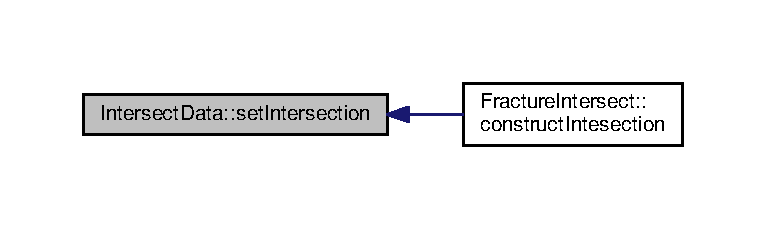
\includegraphics[width=350pt]{classIntersectData_a4dbe681fa68704c9e2bf3f8e290b55f7_icgraph}
\end{center}
\end{figure}


\hypertarget{classIntersectData_a6bcd52066286893ea1f7c36ea841da82}{\index{Intersect\-Data@{Intersect\-Data}!update\-Nodes@{update\-Nodes}}
\index{update\-Nodes@{update\-Nodes}!IntersectData@{Intersect\-Data}}
\subsubsection[{update\-Nodes}]{\setlength{\rightskip}{0pt plus 5cm}void Intersect\-Data\-::update\-Nodes (
\begin{DoxyParamCaption}
\item[{const {\bf Intersect\-Data} \&}]{intersection}
\end{DoxyParamCaption}
)}}\label{classIntersectData_a6bcd52066286893ea1f7c36ea841da82}


Funzione che aggiunge uno degli indici dei nodi di intersezione mancanti. 


\begin{DoxyCode}
69 \{
70     \textcolor{keywordflow}{for} ( size\_type \hyperlink{god__e_8m_a8604be5925f4266ab5ccc69675329c80}{i} = 0; \hyperlink{god__e_8m_a8604be5925f4266ab5ccc69675329c80}{i} < M\_fractures.size(); \hyperlink{god__e_8m_a8604be5925f4266ab5ccc69675329c80}{i}++ )
71     \{
72         \textcolor{keywordflow}{for} ( size\_type j = 0; j < intersection.\hyperlink{classIntersectData_a1c43bd327ed8dedaa89870f60cdb4606}{getFractures} ().size(); j++ )
73         \{
74             \textcolor{keywordflow}{if} ( M\_fractures[ \hyperlink{god__e_8m_a8604be5925f4266ab5ccc69675329c80}{i} ]->getID() == intersection.\hyperlink{classIntersectData_afef7730d6a494464350ebce088e488ee}{getFracture} ( j )->getID () )
75             \{
76                 \textcolor{keywordflow}{if} ( intersection.\hyperlink{classIntersectData_aed138ba9b2e3e33d55999db110871406}{getIntersectionPoint} ().size() != 0 )
77                 \{
78                     M\_intersectionPoint [ \hyperlink{god__e_8m_a8604be5925f4266ab5ccc69675329c80}{i} ] = intersection.
      \hyperlink{classIntersectData_aed138ba9b2e3e33d55999db110871406}{getIntersectionPoint} () [ j ];
79                 \}
80             \}
81         \}
82     \}
83 
84     \textcolor{keywordflow}{return};
85 \}\textcolor{comment}{// updateNodes}
\end{DoxyCode}


Questo è il grafo delle chiamate per questa funzione\-:
\nopagebreak
\begin{figure}[H]
\begin{center}
\leavevmode
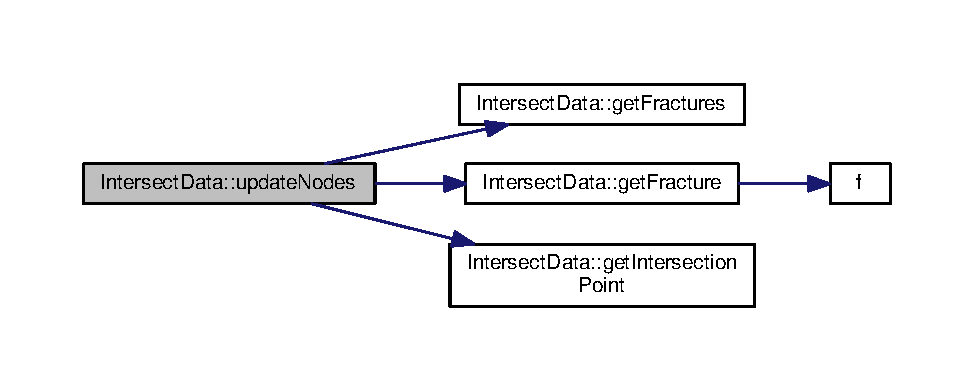
\includegraphics[width=350pt]{classIntersectData_a6bcd52066286893ea1f7c36ea841da82_cgraph}
\end{center}
\end{figure}




La documentazione per questa classe è stata generata a partire dai seguenti file\-:\begin{DoxyCompactItemize}
\item 
include/\hyperlink{IntersectData_8h}{Intersect\-Data.\-h}\item 
src/\hyperlink{IntersectData_8cc}{Intersect\-Data.\-cc}\end{DoxyCompactItemize}

\hypertarget{classLevelSetData}{\section{Riferimenti per la classe Level\-Set\-Data}
\label{classLevelSetData}\index{Level\-Set\-Data@{Level\-Set\-Data}}
}


{\ttfamily \#include $<$Level\-Set\-Data.\-h$>$}

\subsection*{Membri pubblici}
\begin{DoxyCompactItemize}
\item 
\hyperlink{classLevelSetData_a8b2ab7808f47d9a951327891d65e84be}{Level\-Set\-Data} (const Get\-Pot \&data\-File, const std\-::string \&section=\char`\"{}fracture\-Data/\char`\"{}, const std\-::string \&section\-Level\-Set=\char`\"{}level\-Set/\char`\"{})
\item 
scalar\-\_\-type \hyperlink{classLevelSetData_a665241939c12bad26face4d997e655ce}{level\-Set\-Function} (const base\-\_\-node \&\hyperlink{risultati__bastian_8m_a9336ebf25087d91c818ee6e9ec29f8c1}{x})
\begin{DoxyCompactList}\small\item\em Questa funzione definisce il level set che rappresenta la frattura, level set valutato in (x,y). \end{DoxyCompactList}\item 
scalar\-\_\-type \hyperlink{classLevelSetData_a732ae59581206d4f94237e54bc0071e3}{ylevel\-Set\-Function} (const base\-\_\-node \&\hyperlink{risultati__bastian_8m_a9336ebf25087d91c818ee6e9ec29f8c1}{x})
\begin{DoxyCompactList}\small\item\em Questa funzione definisce il level set che rappresenta la frattura, level set valutato in (t,y). \end{DoxyCompactList}\item 
scalar\-\_\-type \hyperlink{classLevelSetData_a60ea6aa9991dfdae4e4a3950ed8db66c}{level\-Set\-Cut\-Function} (const base\-\_\-node \&\hyperlink{risultati__bastian_8m_a9336ebf25087d91c818ee6e9ec29f8c1}{x})
\begin{DoxyCompactList}\small\item\em scalar\-\_\-type level\-Set\-Cut\-Function ( const base\-\_\-node\& x, int num = 0 ) \end{DoxyCompactList}\item 
scalar\-\_\-type \hyperlink{classLevelSetData_aa4cda1cced4bc385d85383b40bbc2631}{y\-\_\-map} (const base\-\_\-node \&\hyperlink{discontinuo_8m_aaccc9105df5383111407fd5b41255e23}{t})
\begin{DoxyCompactList}\small\item\em Questa funzione rappresenta la mappa dalla frattura piatta, y(t). \end{DoxyCompactList}\item 
scalar\-\_\-type \hyperlink{classLevelSetData_ae7f10d3f10b72fbb6f703ba7aa8fe17b}{x\-\_\-map} (const base\-\_\-node \&\hyperlink{discontinuo_8m_aaccc9105df5383111407fd5b41255e23}{t})
\begin{DoxyCompactList}\small\item\em Questa funzione rappresenta la mappa dalla frattura piatta, x(t). \end{DoxyCompactList}\item 
\hyperlink{Core_8h_a4e75b5863535ba1dd79942de2846eff0}{scalar\-Vector\-\_\-\-Type} \hyperlink{classLevelSetData_a40fcfa36de7ac76613284d03690eb54b}{map\-\_\-jac} (const base\-\_\-node \&\hyperlink{risultati__bastian_8m_a9336ebf25087d91c818ee6e9ec29f8c1}{x}, const size\-\_\-type \&num)
\begin{DoxyCompactList}\small\item\em Questa funzione serve per convertire la lunghezza/area degli elementi dalla frattura piatta a quella mappata. \end{DoxyCompactList}\item 
\hyperlink{Core_8h_a4e75b5863535ba1dd79942de2846eff0}{scalar\-Vector\-\_\-\-Type} \hyperlink{classLevelSetData_a674d56690f4e22cbca38bf4b5f176a5e}{normal\-\_\-map} (const base\-\_\-node \&P, const size\-\_\-type \&num)
\begin{DoxyCompactList}\small\item\em Funzione che calcola la normale alla frattura -\/ può anche dipendere da x. \end{DoxyCompactList}\item 
bgeot\-::dim\-\_\-type \hyperlink{classLevelSetData_aa4c3e1f7876cd318e80f5052689fe9e3}{get\-Space\-Dimension} () const 
\item 
std\-::string \hyperlink{classLevelSetData_a672418971ce9b1bf71d3c6bccd278bd7}{get\-Level\-Set\-Function\-String} () const 
\end{DoxyCompactItemize}


\subsection{Documentazione dei costruttori e dei distruttori}
\hypertarget{classLevelSetData_a8b2ab7808f47d9a951327891d65e84be}{\index{Level\-Set\-Data@{Level\-Set\-Data}!Level\-Set\-Data@{Level\-Set\-Data}}
\index{Level\-Set\-Data@{Level\-Set\-Data}!LevelSetData@{Level\-Set\-Data}}
\subsubsection[{Level\-Set\-Data}]{\setlength{\rightskip}{0pt plus 5cm}Level\-Set\-Data\-::\-Level\-Set\-Data (
\begin{DoxyParamCaption}
\item[{const Get\-Pot \&}]{data\-File, }
\item[{const std\-::string \&}]{section = {\ttfamily \char`\"{}fractureData/\char`\"{}}, }
\item[{const std\-::string \&}]{section\-Level\-Set = {\ttfamily \char`\"{}levelSet/\char`\"{}}}
\end{DoxyParamCaption}
)}}\label{classLevelSetData_a8b2ab7808f47d9a951327891d65e84be}

\begin{DoxyCode}
12                                                                :
13                              M\_section ( section ),
14                              M\_sectionLevelSet ( sectionLevelSet ),
15                              M\_spaceDimension ( dataFile ( ( M\_section + \textcolor{stringliteral}{"spaceDimension"} ).data (), 1. ) )
      ,
16                              \textcolor{comment}{// level set}
17                              M\_function ( dataFile ( ( M\_sectionLevelSet + \textcolor{stringliteral}{"levelSet"} ).data (), \textcolor{stringliteral}{"x"} ) ),
18                              M\_xfunction ( dataFile ( ( M\_sectionLevelSet + \textcolor{stringliteral}{"xlevelSet"} ).data (), \textcolor{stringliteral}{"t"} ) ),
19                              M\_yfunction ( dataFile ( ( M\_sectionLevelSet + \textcolor{stringliteral}{"ylevelSet"} ).data (), \textcolor{stringliteral}{"t"} ) ),
20                              M\_cutFunction ( dataFile ( ( M\_sectionLevelSet + \textcolor{stringliteral}{"levelSetCut"} ).data (), \textcolor{stringliteral}{"-1"}
       ) ),
21                              M\_x\_map ( dataFile ( ( M\_sectionLevelSet + \textcolor{stringliteral}{"xMap"} ).data (), \textcolor{stringliteral}{"1"} ) ),
22                              M\_y\_map ( dataFile ( ( M\_sectionLevelSet + \textcolor{stringliteral}{"yMap"} ).data (), \textcolor{stringliteral}{"1"} ) ),
23                              M\_map\_jac ( dataFile ( ( M\_sectionLevelSet + \textcolor{stringliteral}{"jacMap"} ).data (), \textcolor{stringliteral}{"1"} ) ),
24                              M\_normal\_map ( dataFile ( ( M\_sectionLevelSet + \textcolor{stringliteral}{"normalMap"} ).data (), \textcolor{stringliteral}{"1"} ) )
25 \{\}
\end{DoxyCode}


\subsection{Documentazione delle funzioni membro}
\hypertarget{classLevelSetData_a672418971ce9b1bf71d3c6bccd278bd7}{\index{Level\-Set\-Data@{Level\-Set\-Data}!get\-Level\-Set\-Function\-String@{get\-Level\-Set\-Function\-String}}
\index{get\-Level\-Set\-Function\-String@{get\-Level\-Set\-Function\-String}!LevelSetData@{Level\-Set\-Data}}
\subsubsection[{get\-Level\-Set\-Function\-String}]{\setlength{\rightskip}{0pt plus 5cm}std\-::string Level\-Set\-Data\-::get\-Level\-Set\-Function\-String (
\begin{DoxyParamCaption}
{}
\end{DoxyParamCaption}
) const\hspace{0.3cm}{\ttfamily [inline]}}}\label{classLevelSetData_a672418971ce9b1bf71d3c6bccd278bd7}

\begin{DoxyCode}
92     \{
93         \textcolor{keywordflow}{return} M\_yfunction;
94     \}
\end{DoxyCode}
\hypertarget{classLevelSetData_aa4c3e1f7876cd318e80f5052689fe9e3}{\index{Level\-Set\-Data@{Level\-Set\-Data}!get\-Space\-Dimension@{get\-Space\-Dimension}}
\index{get\-Space\-Dimension@{get\-Space\-Dimension}!LevelSetData@{Level\-Set\-Data}}
\subsubsection[{get\-Space\-Dimension}]{\setlength{\rightskip}{0pt plus 5cm}bgeot\-::dim\-\_\-type Level\-Set\-Data\-::get\-Space\-Dimension (
\begin{DoxyParamCaption}
{}
\end{DoxyParamCaption}
) const\hspace{0.3cm}{\ttfamily [inline]}}}\label{classLevelSetData_aa4c3e1f7876cd318e80f5052689fe9e3}

\begin{DoxyCode}
87     \{
88         \textcolor{keywordflow}{return} M\_spaceDimension;
89     \}
\end{DoxyCode}
\hypertarget{classLevelSetData_a60ea6aa9991dfdae4e4a3950ed8db66c}{\index{Level\-Set\-Data@{Level\-Set\-Data}!level\-Set\-Cut\-Function@{level\-Set\-Cut\-Function}}
\index{level\-Set\-Cut\-Function@{level\-Set\-Cut\-Function}!LevelSetData@{Level\-Set\-Data}}
\subsubsection[{level\-Set\-Cut\-Function}]{\setlength{\rightskip}{0pt plus 5cm}scalar\-\_\-type Level\-Set\-Data\-::level\-Set\-Cut\-Function (
\begin{DoxyParamCaption}
\item[{const base\-\_\-node \&}]{x}
\end{DoxyParamCaption}
)}}\label{classLevelSetData_a60ea6aa9991dfdae4e4a3950ed8db66c}


scalar\-\_\-type level\-Set\-Cut\-Function ( const base\-\_\-node\& x, int num = 0 ) 

Questa funzione definisce il level set che rappresenta la frattura, se per caso voglio \char`\"{}tagliare la frattura\char`\"{}. 
\begin{DoxyParams}{Parametri}
{\em base\-\_\-node\&} & x\-: nodo in coordinate ( t, y ) in cui valutare il levelset \\
\hline
\end{DoxyParams}
\begin{DoxyReturn}{Restituisce}
scalar\-\_\-type\-: valore del levelset nel nodo x 
\end{DoxyReturn}

\begin{DoxyCode}
50 \{
51     M\_parser.\hyperlink{classLifeV_1_1Parser_ac05769e836a0dc95d9c020df361a5194}{setString} ( M\_cutFunction );
52     M\_parser.\hyperlink{classLifeV_1_1Parser_aa2b362e12b8feb60231705d499c9fbae}{setVariable} ( \textcolor{stringliteral}{"t"}, \hyperlink{discontinuo_8m_aaccc9105df5383111407fd5b41255e23}{t} [ 0 ] );
53     M\_parser.\hyperlink{classLifeV_1_1Parser_aa2b362e12b8feb60231705d499c9fbae}{setVariable} ( \textcolor{stringliteral}{"y"}, \hyperlink{discontinuo_8m_aaccc9105df5383111407fd5b41255e23}{t} [ 1 ] );
54 
55     \textcolor{keywordflow}{return} M\_parser.\hyperlink{classLifeV_1_1Parser_a51d84fd4ae6d420620e7beee58fad673}{evaluate} ();
56 \}
\end{DoxyCode}


Questo è il grafo delle chiamate per questa funzione\-:
\nopagebreak
\begin{figure}[H]
\begin{center}
\leavevmode
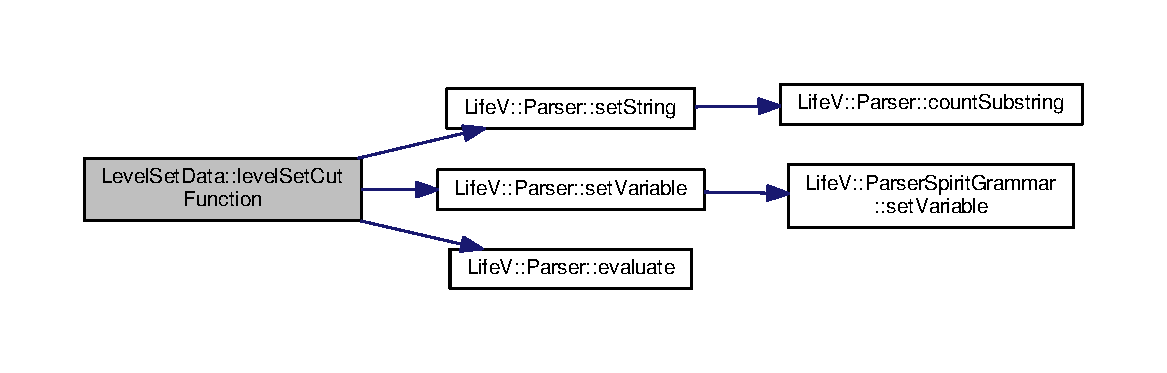
\includegraphics[width=350pt]{classLevelSetData_a60ea6aa9991dfdae4e4a3950ed8db66c_cgraph}
\end{center}
\end{figure}


\hypertarget{classLevelSetData_a665241939c12bad26face4d997e655ce}{\index{Level\-Set\-Data@{Level\-Set\-Data}!level\-Set\-Function@{level\-Set\-Function}}
\index{level\-Set\-Function@{level\-Set\-Function}!LevelSetData@{Level\-Set\-Data}}
\subsubsection[{level\-Set\-Function}]{\setlength{\rightskip}{0pt plus 5cm}scalar\-\_\-type Level\-Set\-Data\-::level\-Set\-Function (
\begin{DoxyParamCaption}
\item[{const base\-\_\-node \&}]{x}
\end{DoxyParamCaption}
)}}\label{classLevelSetData_a665241939c12bad26face4d997e655ce}


Questa funzione definisce il level set che rappresenta la frattura, level set valutato in (x,y). 


\begin{DoxyParams}{Parametri}
{\em base\-\_\-node\&} & x\-: nodo in coordinate ( x, y ) in cui valutare il levelset \\
\hline
\end{DoxyParams}
\begin{DoxyReturn}{Restituisce}
scalar\-\_\-type\-: valore del levelset nel nodo x 
\end{DoxyReturn}

\begin{DoxyCode}
30 \{
31     M\_parser.\hyperlink{classLifeV_1_1Parser_ac05769e836a0dc95d9c020df361a5194}{setString} ( M\_function );
32     M\_parser.\hyperlink{classLifeV_1_1Parser_aa2b362e12b8feb60231705d499c9fbae}{setVariable} ( \textcolor{stringliteral}{"x"}, \hyperlink{discontinuo_8m_aaccc9105df5383111407fd5b41255e23}{t} [ 0 ] );
33     M\_parser.\hyperlink{classLifeV_1_1Parser_aa2b362e12b8feb60231705d499c9fbae}{setVariable} ( \textcolor{stringliteral}{"y"}, \hyperlink{discontinuo_8m_aaccc9105df5383111407fd5b41255e23}{t} [ 1 ] );
34 
35     \textcolor{keywordflow}{return} M\_parser.\hyperlink{classLifeV_1_1Parser_a51d84fd4ae6d420620e7beee58fad673}{evaluate} ();
36 \}
\end{DoxyCode}


Questo è il grafo delle chiamate per questa funzione\-:
\nopagebreak
\begin{figure}[H]
\begin{center}
\leavevmode
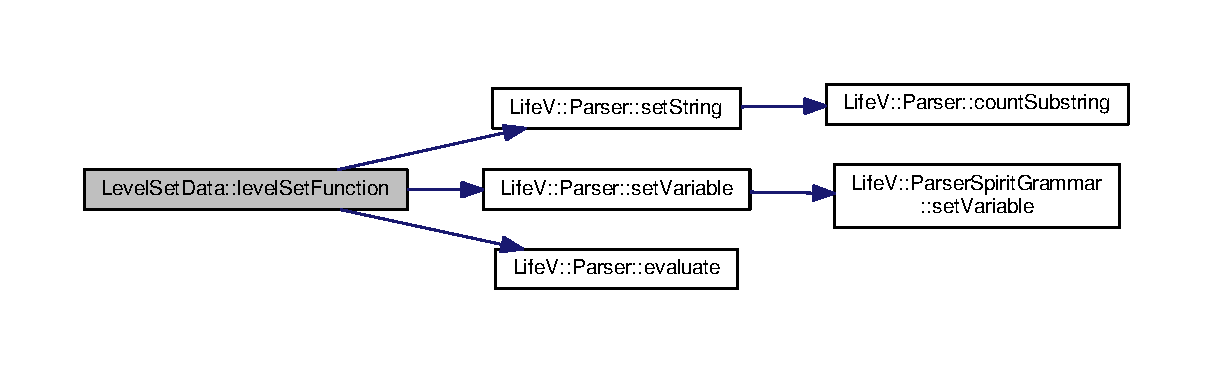
\includegraphics[width=350pt]{classLevelSetData_a665241939c12bad26face4d997e655ce_cgraph}
\end{center}
\end{figure}


\hypertarget{classLevelSetData_a40fcfa36de7ac76613284d03690eb54b}{\index{Level\-Set\-Data@{Level\-Set\-Data}!map\-\_\-jac@{map\-\_\-jac}}
\index{map\-\_\-jac@{map\-\_\-jac}!LevelSetData@{Level\-Set\-Data}}
\subsubsection[{map\-\_\-jac}]{\setlength{\rightskip}{0pt plus 5cm}{\bf scalar\-Vector\-\_\-\-Type} Level\-Set\-Data\-::map\-\_\-jac (
\begin{DoxyParamCaption}
\item[{const base\-\_\-node \&}]{x, }
\item[{const size\-\_\-type \&}]{num}
\end{DoxyParamCaption}
)}}\label{classLevelSetData_a40fcfa36de7ac76613284d03690eb54b}


Questa funzione serve per convertire la lunghezza/area degli elementi dalla frattura piatta a quella mappata. 


\begin{DoxyCode}
78 \{
79     \hyperlink{Core_8h_a4e75b5863535ba1dd79942de2846eff0}{scalarVector\_Type} \hyperlink{classLevelSetData_a40fcfa36de7ac76613284d03690eb54b}{map\_jac} ( num, 0. );
80 
81     M\_parser.\hyperlink{classLifeV_1_1Parser_ac05769e836a0dc95d9c020df361a5194}{setString} ( M\_map\_jac );
82     M\_parser.\hyperlink{classLifeV_1_1Parser_aa2b362e12b8feb60231705d499c9fbae}{setVariable} ( \textcolor{stringliteral}{"x"}, \hyperlink{confronto_8m_ad2e52d4a42a755ccd73c8de47175afa3}{x} [ 0 ] );
83     M\_parser.\hyperlink{classLifeV_1_1Parser_aa2b362e12b8feb60231705d499c9fbae}{setVariable} ( \textcolor{stringliteral}{"y"}, \hyperlink{confronto_8m_ad2e52d4a42a755ccd73c8de47175afa3}{x} [ 1 ] );
84 
85     \textcolor{keywordflow}{for} ( size\_type \hyperlink{god__e_8m_a8604be5925f4266ab5ccc69675329c80}{i} = 0; \hyperlink{god__e_8m_a8604be5925f4266ab5ccc69675329c80}{i} < num; ++\hyperlink{god__e_8m_a8604be5925f4266ab5ccc69675329c80}{i} )
86     \{
87         \hyperlink{classLevelSetData_a40fcfa36de7ac76613284d03690eb54b}{map\_jac} [ \hyperlink{god__e_8m_a8604be5925f4266ab5ccc69675329c80}{i} ] = M\_parser.\hyperlink{classLifeV_1_1Parser_a51d84fd4ae6d420620e7beee58fad673}{evaluate} ( \hyperlink{god__e_8m_a8604be5925f4266ab5ccc69675329c80}{i} );
88     \}
89 
90     \textcolor{keywordflow}{return} \hyperlink{classLevelSetData_a40fcfa36de7ac76613284d03690eb54b}{map\_jac};
91 \}
\end{DoxyCode}


Questo è il grafo delle chiamate per questa funzione\-:
\nopagebreak
\begin{figure}[H]
\begin{center}
\leavevmode
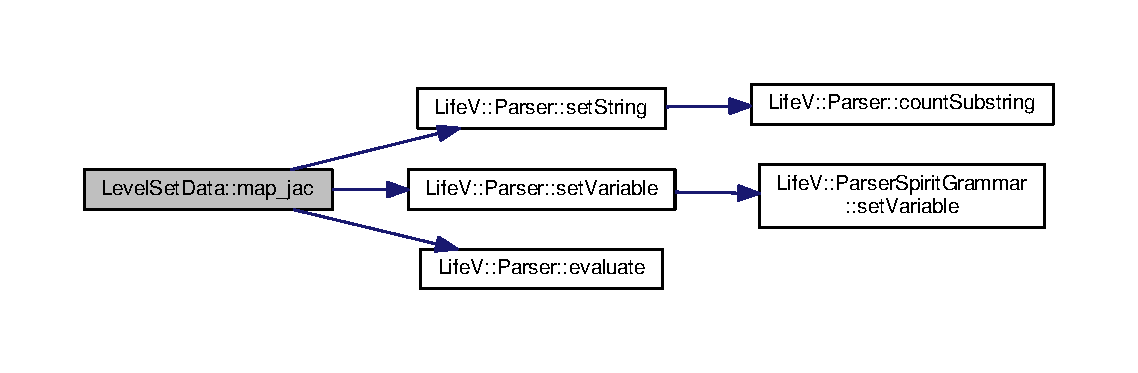
\includegraphics[width=350pt]{classLevelSetData_a40fcfa36de7ac76613284d03690eb54b_cgraph}
\end{center}
\end{figure}


\hypertarget{classLevelSetData_a674d56690f4e22cbca38bf4b5f176a5e}{\index{Level\-Set\-Data@{Level\-Set\-Data}!normal\-\_\-map@{normal\-\_\-map}}
\index{normal\-\_\-map@{normal\-\_\-map}!LevelSetData@{Level\-Set\-Data}}
\subsubsection[{normal\-\_\-map}]{\setlength{\rightskip}{0pt plus 5cm}{\bf scalar\-Vector\-\_\-\-Type} Level\-Set\-Data\-::normal\-\_\-map (
\begin{DoxyParamCaption}
\item[{const base\-\_\-node \&}]{P, }
\item[{const size\-\_\-type \&}]{num}
\end{DoxyParamCaption}
)}}\label{classLevelSetData_a674d56690f4e22cbca38bf4b5f176a5e}


Funzione che calcola la normale alla frattura -\/ può anche dipendere da x. 


\begin{DoxyCode}
96 \{
97     \hyperlink{Core_8h_a4e75b5863535ba1dd79942de2846eff0}{scalarVector\_Type} \hyperlink{classLevelSetData_a674d56690f4e22cbca38bf4b5f176a5e}{normal\_map} ( num + 1, 0. );
98 
99     M\_parser.\hyperlink{classLifeV_1_1Parser_ac05769e836a0dc95d9c020df361a5194}{setString} ( M\_map\_jac );
100     M\_parser.\hyperlink{classLifeV_1_1Parser_aa2b362e12b8feb60231705d499c9fbae}{setVariable} ( \textcolor{stringliteral}{"x"}, \hyperlink{confronto_8m_ad2e52d4a42a755ccd73c8de47175afa3}{x} [ 0 ] );
101     M\_parser.\hyperlink{classLifeV_1_1Parser_aa2b362e12b8feb60231705d499c9fbae}{setVariable} ( \textcolor{stringliteral}{"y"}, \hyperlink{confronto_8m_ad2e52d4a42a755ccd73c8de47175afa3}{x} [ 1 ] );
102 
103     \textcolor{keywordflow}{for} ( size\_type \hyperlink{god__e_8m_a8604be5925f4266ab5ccc69675329c80}{i} = 0; \hyperlink{god__e_8m_a8604be5925f4266ab5ccc69675329c80}{i} < num + 1; ++\hyperlink{god__e_8m_a8604be5925f4266ab5ccc69675329c80}{i} )
104     \{
105         \hyperlink{classLevelSetData_a674d56690f4e22cbca38bf4b5f176a5e}{normal\_map} [ \hyperlink{god__e_8m_a8604be5925f4266ab5ccc69675329c80}{i} ] = M\_parser.\hyperlink{classLifeV_1_1Parser_a51d84fd4ae6d420620e7beee58fad673}{evaluate} ( \hyperlink{god__e_8m_a8604be5925f4266ab5ccc69675329c80}{i} );
106     \}
107 
108     \textcolor{keywordflow}{return} \hyperlink{classLevelSetData_a674d56690f4e22cbca38bf4b5f176a5e}{normal\_map};
109 \}
\end{DoxyCode}


Questo è il grafo delle chiamate per questa funzione\-:
\nopagebreak
\begin{figure}[H]
\begin{center}
\leavevmode
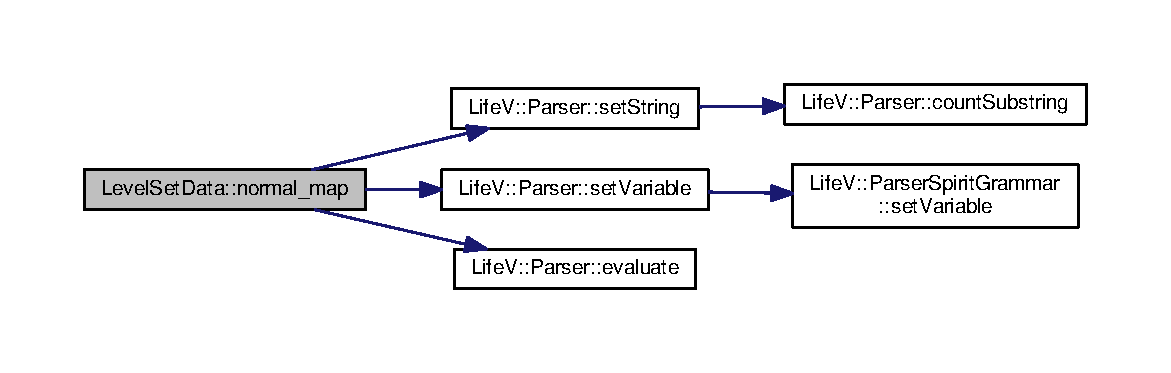
\includegraphics[width=350pt]{classLevelSetData_a674d56690f4e22cbca38bf4b5f176a5e_cgraph}
\end{center}
\end{figure}


\hypertarget{classLevelSetData_ae7f10d3f10b72fbb6f703ba7aa8fe17b}{\index{Level\-Set\-Data@{Level\-Set\-Data}!x\-\_\-map@{x\-\_\-map}}
\index{x\-\_\-map@{x\-\_\-map}!LevelSetData@{Level\-Set\-Data}}
\subsubsection[{x\-\_\-map}]{\setlength{\rightskip}{0pt plus 5cm}scalar\-\_\-type Level\-Set\-Data\-::x\-\_\-map (
\begin{DoxyParamCaption}
\item[{const base\-\_\-node \&}]{t}
\end{DoxyParamCaption}
)}}\label{classLevelSetData_ae7f10d3f10b72fbb6f703ba7aa8fe17b}


Questa funzione rappresenta la mappa dalla frattura piatta, x(t). 


\begin{DoxyCode}
69 \{
70     M\_parser.\hyperlink{classLifeV_1_1Parser_ac05769e836a0dc95d9c020df361a5194}{setString} ( M\_x\_map );
71     M\_parser.\hyperlink{classLifeV_1_1Parser_aa2b362e12b8feb60231705d499c9fbae}{setVariable} ( \textcolor{stringliteral}{"t"}, \hyperlink{discontinuo_8m_aaccc9105df5383111407fd5b41255e23}{t} [ 0 ] );
72 
73     \textcolor{keywordflow}{return} M\_parser.\hyperlink{classLifeV_1_1Parser_a51d84fd4ae6d420620e7beee58fad673}{evaluate} ();
74 \}
\end{DoxyCode}


Questo è il grafo delle chiamate per questa funzione\-:
\nopagebreak
\begin{figure}[H]
\begin{center}
\leavevmode
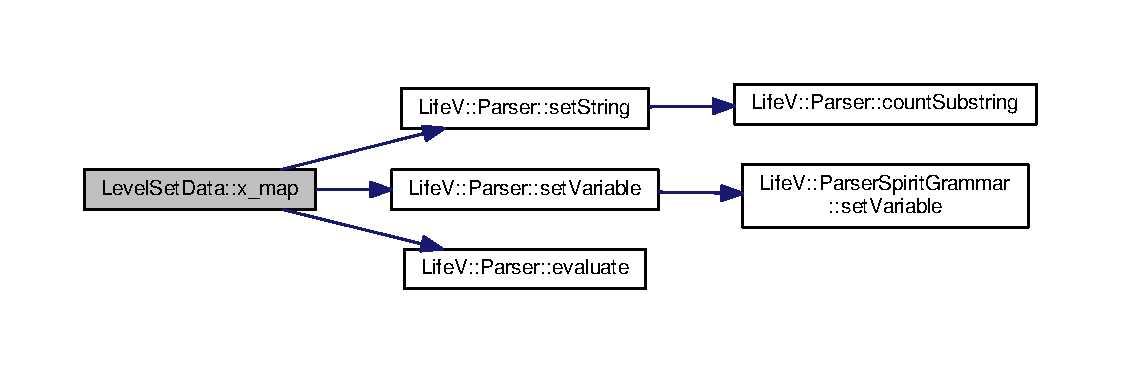
\includegraphics[width=350pt]{classLevelSetData_ae7f10d3f10b72fbb6f703ba7aa8fe17b_cgraph}
\end{center}
\end{figure}


\hypertarget{classLevelSetData_aa4cda1cced4bc385d85383b40bbc2631}{\index{Level\-Set\-Data@{Level\-Set\-Data}!y\-\_\-map@{y\-\_\-map}}
\index{y\-\_\-map@{y\-\_\-map}!LevelSetData@{Level\-Set\-Data}}
\subsubsection[{y\-\_\-map}]{\setlength{\rightskip}{0pt plus 5cm}scalar\-\_\-type Level\-Set\-Data\-::y\-\_\-map (
\begin{DoxyParamCaption}
\item[{const base\-\_\-node \&}]{t}
\end{DoxyParamCaption}
)}}\label{classLevelSetData_aa4cda1cced4bc385d85383b40bbc2631}


Questa funzione rappresenta la mappa dalla frattura piatta, y(t). 


\begin{DoxyCode}
60 \{
61     M\_parser.\hyperlink{classLifeV_1_1Parser_ac05769e836a0dc95d9c020df361a5194}{setString} ( M\_y\_map );
62     M\_parser.\hyperlink{classLifeV_1_1Parser_aa2b362e12b8feb60231705d499c9fbae}{setVariable} ( \textcolor{stringliteral}{"t"}, \hyperlink{discontinuo_8m_aaccc9105df5383111407fd5b41255e23}{t} [ 0 ] );
63 
64     \textcolor{keywordflow}{return} M\_parser.\hyperlink{classLifeV_1_1Parser_a51d84fd4ae6d420620e7beee58fad673}{evaluate} ();
65 \}
\end{DoxyCode}


Questo è il grafo delle chiamate per questa funzione\-:
\nopagebreak
\begin{figure}[H]
\begin{center}
\leavevmode
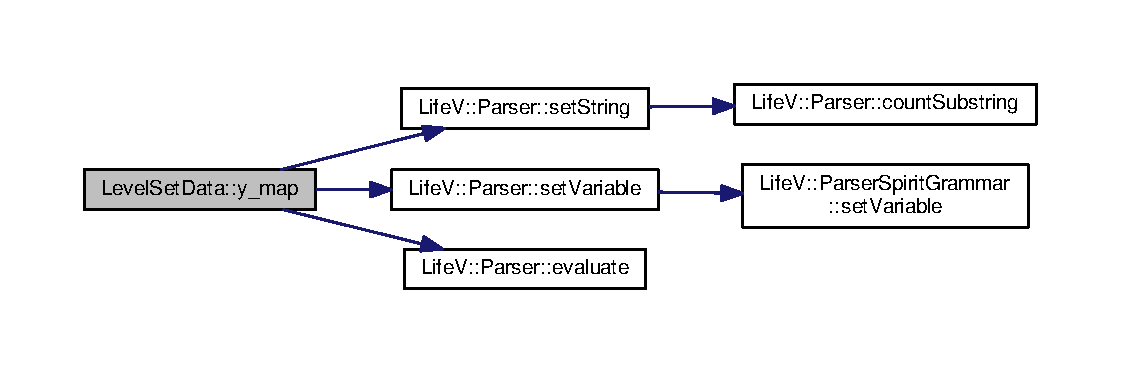
\includegraphics[width=350pt]{classLevelSetData_aa4cda1cced4bc385d85383b40bbc2631_cgraph}
\end{center}
\end{figure}


\hypertarget{classLevelSetData_a732ae59581206d4f94237e54bc0071e3}{\index{Level\-Set\-Data@{Level\-Set\-Data}!ylevel\-Set\-Function@{ylevel\-Set\-Function}}
\index{ylevel\-Set\-Function@{ylevel\-Set\-Function}!LevelSetData@{Level\-Set\-Data}}
\subsubsection[{ylevel\-Set\-Function}]{\setlength{\rightskip}{0pt plus 5cm}scalar\-\_\-type Level\-Set\-Data\-::ylevel\-Set\-Function (
\begin{DoxyParamCaption}
\item[{const base\-\_\-node \&}]{x}
\end{DoxyParamCaption}
)}}\label{classLevelSetData_a732ae59581206d4f94237e54bc0071e3}


Questa funzione definisce il level set che rappresenta la frattura, level set valutato in (t,y). 


\begin{DoxyParams}{Parametri}
{\em base\-\_\-node\&} & x\-: nodo in coordinate ( t, y ) in cui valutare il levelset \\
\hline
\end{DoxyParams}
\begin{DoxyReturn}{Restituisce}
scalar\-\_\-type\-: valore del levelset nel nodo x 
\end{DoxyReturn}

\begin{DoxyCode}
40 \{
41     M\_parser.\hyperlink{classLifeV_1_1Parser_ac05769e836a0dc95d9c020df361a5194}{setString} ( M\_yfunction );
42     M\_parser.\hyperlink{classLifeV_1_1Parser_aa2b362e12b8feb60231705d499c9fbae}{setVariable} ( \textcolor{stringliteral}{"t"}, \hyperlink{discontinuo_8m_aaccc9105df5383111407fd5b41255e23}{t} [ 0 ] );
43     M\_parser.\hyperlink{classLifeV_1_1Parser_aa2b362e12b8feb60231705d499c9fbae}{setVariable} ( \textcolor{stringliteral}{"y"}, \hyperlink{discontinuo_8m_aaccc9105df5383111407fd5b41255e23}{t} [ 1 ] );
44 
45     \textcolor{keywordflow}{return} M\_parser.\hyperlink{classLifeV_1_1Parser_a51d84fd4ae6d420620e7beee58fad673}{evaluate} ();
46 \}
\end{DoxyCode}


Questo è il grafo delle chiamate per questa funzione\-:
\nopagebreak
\begin{figure}[H]
\begin{center}
\leavevmode
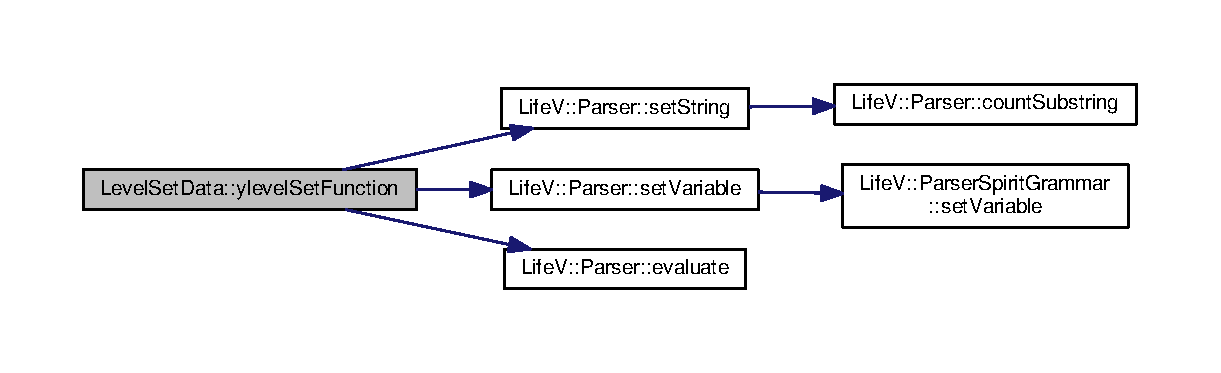
\includegraphics[width=350pt]{classLevelSetData_a732ae59581206d4f94237e54bc0071e3_cgraph}
\end{center}
\end{figure}




La documentazione per questa classe è stata generata a partire dai seguenti file\-:\begin{DoxyCompactItemize}
\item 
include/\hyperlink{LevelSetData_8h}{Level\-Set\-Data.\-h}\item 
src/\hyperlink{LevelSetData_8cc}{Level\-Set\-Data.\-cc}\end{DoxyCompactItemize}

\hypertarget{classLevelSetHandler}{\section{Riferimenti per la classe Level\-Set\-Handler}
\label{classLevelSetHandler}\index{Level\-Set\-Handler@{Level\-Set\-Handler}}
}


{\ttfamily \#include $<$Level\-Set\-Handler.\-h$>$}

\subsection*{Membri pubblici}
\begin{DoxyCompactItemize}
\item 
\hyperlink{classLevelSetHandler_a9dbe142d7d4f677abe8c204714c004ed}{Level\-Set\-Handler} (const Get\-Pot \&data\-File, const std\-::string \&section=\char`\"{}fracture\-Data/\char`\"{}, const std\-::string \&section\-Level\-Set=\char`\"{}level\-Set/\char`\"{})
\item 
\hyperlink{LevelSetData_8h_a7750f14ec1c622b3c69aa0c5c2894972}{Level\-Set\-Data\-Ptr\-\_\-\-Type} \& \hyperlink{classLevelSetHandler_ab24897cb969210d278f54d94fd8f8977}{get\-Data} ()
\end{DoxyCompactItemize}


\subsection{Documentazione dei costruttori e dei distruttori}
\hypertarget{classLevelSetHandler_a9dbe142d7d4f677abe8c204714c004ed}{\index{Level\-Set\-Handler@{Level\-Set\-Handler}!Level\-Set\-Handler@{Level\-Set\-Handler}}
\index{Level\-Set\-Handler@{Level\-Set\-Handler}!LevelSetHandler@{Level\-Set\-Handler}}
\subsubsection[{Level\-Set\-Handler}]{\setlength{\rightskip}{0pt plus 5cm}Level\-Set\-Handler\-::\-Level\-Set\-Handler (
\begin{DoxyParamCaption}
\item[{const Get\-Pot \&}]{data\-File, }
\item[{const std\-::string \&}]{section = {\ttfamily \char`\"{}fractureData/\char`\"{}}, }
\item[{const std\-::string \&}]{section\-Level\-Set = {\ttfamily \char`\"{}levelSet/\char`\"{}}}
\end{DoxyParamCaption}
)}}\label{classLevelSetHandler_a9dbe142d7d4f677abe8c204714c004ed}

\begin{DoxyCode}
11                                                                      :
12                                    M\_Data ( \textcolor{keyword}{new} \hyperlink{classLevelSetData}{LevelSetData\_Type} ( dataFile, section, 
      sectionLevelSet ) )
13 \{\}
\end{DoxyCode}


\subsection{Documentazione delle funzioni membro}
\hypertarget{classLevelSetHandler_ab24897cb969210d278f54d94fd8f8977}{\index{Level\-Set\-Handler@{Level\-Set\-Handler}!get\-Data@{get\-Data}}
\index{get\-Data@{get\-Data}!LevelSetHandler@{Level\-Set\-Handler}}
\subsubsection[{get\-Data}]{\setlength{\rightskip}{0pt plus 5cm}{\bf Level\-Set\-Data\-Ptr\-\_\-\-Type}\& Level\-Set\-Handler\-::get\-Data (
\begin{DoxyParamCaption}
{}
\end{DoxyParamCaption}
)\hspace{0.3cm}{\ttfamily [inline]}}}\label{classLevelSetHandler_ab24897cb969210d278f54d94fd8f8977}

\begin{DoxyCode}
30     \{
31         \textcolor{keywordflow}{return} M\_Data;
32     \}
\end{DoxyCode}


La documentazione per questa classe è stata generata a partire dai seguenti file\-:\begin{DoxyCompactItemize}
\item 
include/\hyperlink{LevelSetHandler_8h}{Level\-Set\-Handler.\-h}\item 
src/\hyperlink{LevelSetHandler_8cc}{Level\-Set\-Handler.\-cc}\end{DoxyCompactItemize}

\hypertarget{classLifeV_1_1Parser}{\section{Riferimenti per la classe Life\-V\-:\-:Parser}
\label{classLifeV_1_1Parser}\index{Life\-V\-::\-Parser@{Life\-V\-::\-Parser}}
}


\hyperlink{classLifeV_1_1Parser}{Parser} -\/ A string parser for algebraic expressions.  




{\ttfamily \#include $<$Parser.\-h$>$}

\subsection*{Tipi pubblici}
\begin{Indent}{\bf Public Types}\par
\begin{DoxyCompactItemize}
\item 
typedef std\-::vector$<$ std\-::string $>$ \hyperlink{classLifeV_1_1Parser_af87d4a11879da16a0bba7bf81f98b957}{strings\-Vector\-\_\-\-Type}
\item 
typedef std\-::string\-::const\-\_\-iterator \hyperlink{classLifeV_1_1Parser_a9491c77a9093b41468ca54b865c893ff}{string\-Iterator\-\_\-\-Type}
\item 
typedef \hyperlink{classLifeV_1_1ParserSpiritGrammar}{Parser\-Spirit\-Grammar}\\*
$<$ \hyperlink{classLifeV_1_1Parser_a9491c77a9093b41468ca54b865c893ff}{string\-Iterator\-\_\-\-Type} $>$ \hyperlink{classLifeV_1_1Parser_ae9a67e24d777a1f962026f5e1274b61a}{calculator\-\_\-\-Type}
\item 
typedef \\*
\hyperlink{classLifeV_1_1ParserSpiritGrammar_a98dabec1a4a9a743a1d3b35e994cec7c}{calculator\-\_\-\-Type\-::results\-\_\-\-Type} \hyperlink{classLifeV_1_1Parser_a9e5861cc337d7534e8641b1709d193db}{results\-\_\-\-Type}
\end{DoxyCompactItemize}
\end{Indent}
\subsection*{Membri pubblici}
\begin{Indent}{\bf Constructors \& Destructor}\par
\begin{DoxyCompactItemize}
\item 
\hyperlink{classLifeV_1_1Parser_a439ecd746d503e75b6e07f2933a665dc}{Parser} ()
\begin{DoxyCompactList}\small\item\em Empty constructor (it needs a manual call to set\-String) \end{DoxyCompactList}\item 
\hyperlink{classLifeV_1_1Parser_a6acf25b7222f0c65d1414611236d1820}{Parser} (const std\-::string \&string)
\begin{DoxyCompactList}\small\item\em Constructor. \end{DoxyCompactList}\item 
\hyperlink{classLifeV_1_1Parser_a0f7c4d10928fd2139e76baf44996b610}{Parser} (const \hyperlink{classLifeV_1_1Parser}{Parser} \&parser)
\begin{DoxyCompactList}\small\item\em Copy constructor. \end{DoxyCompactList}\item 
virtual \hyperlink{classLifeV_1_1Parser_a34d16f77f23cf33b3bc3f8293ed0e2ed}{$\sim$\-Parser} ()
\begin{DoxyCompactList}\small\item\em Destructor. \end{DoxyCompactList}\end{DoxyCompactItemize}
\end{Indent}
\begin{Indent}{\bf Operators}\par
\begin{DoxyCompactItemize}
\item 
\hyperlink{classLifeV_1_1Parser}{Parser} \& \hyperlink{classLifeV_1_1Parser_a257904e57f46427a5bd7c9f80e658c2d}{operator=} (const \hyperlink{classLifeV_1_1Parser}{Parser} \&parser)
\begin{DoxyCompactList}\small\item\em Operator =. \end{DoxyCompactList}\end{DoxyCompactItemize}
\end{Indent}
\begin{Indent}{\bf Methods}\par
\begin{DoxyCompactItemize}
\item 
const \hyperlink{namespaceLifeV_ad58c7402b26e5087b634b25d029c9c32}{Real} \& \hyperlink{classLifeV_1_1Parser_a51d84fd4ae6d420620e7beee58fad673}{evaluate} (const \hyperlink{namespaceLifeV_a7c0e64679fcd30daa5471b87a57601e9}{I\-D} \&id=0)
\item 
\hyperlink{namespaceLifeV_a4bd093cf6b0d5b57b2d89e0e90d610b7}{U\-Int} \hyperlink{classLifeV_1_1Parser_a37ae3af9abcf72ca8e1537ec771b523a}{count\-Substring} (const std\-::string \&substring)
\item 
void \hyperlink{classLifeV_1_1Parser_acbc44ff1f0b0074f071ea264a95cb9e7}{clear\-Variables} ()
\begin{DoxyCompactList}\small\item\em Clear all the variables. \end{DoxyCompactList}\end{DoxyCompactItemize}
\end{Indent}
\begin{Indent}{\bf Set Methods}\par
\begin{DoxyCompactItemize}
\item 
void \hyperlink{classLifeV_1_1Parser_ac05769e836a0dc95d9c020df361a5194}{set\-String} (const std\-::string \&string, const std\-::string \&string\-Separator=\char`\"{};\char`\"{})
\item 
void \hyperlink{classLifeV_1_1Parser_aa2b362e12b8feb60231705d499c9fbae}{set\-Variable} (const std\-::string \&name, const \hyperlink{namespaceLifeV_ad58c7402b26e5087b634b25d029c9c32}{Real} \&value)
\end{DoxyCompactItemize}
\end{Indent}
\begin{Indent}{\bf Get Methods}\par
\begin{DoxyCompactItemize}
\item 
const \hyperlink{namespaceLifeV_ad58c7402b26e5087b634b25d029c9c32}{Real} \& \hyperlink{classLifeV_1_1Parser_a9fa902c13c73a3b1bc6db2b5e5c5c93d}{variable} (const std\-::string \&name)
\end{DoxyCompactItemize}
\end{Indent}


\subsection{Descrizione dettagliata}
\hyperlink{classLifeV_1_1Parser}{Parser} -\/ A string parser for algebraic expressions. 

\begin{DoxyAuthor}{Autore}
(s) Cristiano Malossi, Gilles Fourestey
\end{DoxyAuthor}
See {\ttfamily \hyperlink{classLifeV_1_1ParserSpiritGrammar}{Parser\-Spirit\-Grammar}} class for more details. 

\subsection{Documentazione delle ridefinizioni dei tipi (typedef)}
\hypertarget{classLifeV_1_1Parser_ae9a67e24d777a1f962026f5e1274b61a}{\index{Life\-V\-::\-Parser@{Life\-V\-::\-Parser}!calculator\-\_\-\-Type@{calculator\-\_\-\-Type}}
\index{calculator\-\_\-\-Type@{calculator\-\_\-\-Type}!LifeV::Parser@{Life\-V\-::\-Parser}}
\subsubsection[{calculator\-\_\-\-Type}]{\setlength{\rightskip}{0pt plus 5cm}typedef {\bf Parser\-Spirit\-Grammar}$<$ {\bf string\-Iterator\-\_\-\-Type} $>$ {\bf Life\-V\-::\-Parser\-::calculator\-\_\-\-Type}}}\label{classLifeV_1_1Parser_ae9a67e24d777a1f962026f5e1274b61a}
\hypertarget{classLifeV_1_1Parser_a9e5861cc337d7534e8641b1709d193db}{\index{Life\-V\-::\-Parser@{Life\-V\-::\-Parser}!results\-\_\-\-Type@{results\-\_\-\-Type}}
\index{results\-\_\-\-Type@{results\-\_\-\-Type}!LifeV::Parser@{Life\-V\-::\-Parser}}
\subsubsection[{results\-\_\-\-Type}]{\setlength{\rightskip}{0pt plus 5cm}typedef {\bf calculator\-\_\-\-Type\-::results\-\_\-\-Type} {\bf Life\-V\-::\-Parser\-::results\-\_\-\-Type}}}\label{classLifeV_1_1Parser_a9e5861cc337d7534e8641b1709d193db}
\hypertarget{classLifeV_1_1Parser_a9491c77a9093b41468ca54b865c893ff}{\index{Life\-V\-::\-Parser@{Life\-V\-::\-Parser}!string\-Iterator\-\_\-\-Type@{string\-Iterator\-\_\-\-Type}}
\index{string\-Iterator\-\_\-\-Type@{string\-Iterator\-\_\-\-Type}!LifeV::Parser@{Life\-V\-::\-Parser}}
\subsubsection[{string\-Iterator\-\_\-\-Type}]{\setlength{\rightskip}{0pt plus 5cm}typedef std\-::string\-::const\-\_\-iterator {\bf Life\-V\-::\-Parser\-::string\-Iterator\-\_\-\-Type}}}\label{classLifeV_1_1Parser_a9491c77a9093b41468ca54b865c893ff}
\hypertarget{classLifeV_1_1Parser_af87d4a11879da16a0bba7bf81f98b957}{\index{Life\-V\-::\-Parser@{Life\-V\-::\-Parser}!strings\-Vector\-\_\-\-Type@{strings\-Vector\-\_\-\-Type}}
\index{strings\-Vector\-\_\-\-Type@{strings\-Vector\-\_\-\-Type}!LifeV::Parser@{Life\-V\-::\-Parser}}
\subsubsection[{strings\-Vector\-\_\-\-Type}]{\setlength{\rightskip}{0pt plus 5cm}typedef std\-::vector$<$ std\-::string $>$ {\bf Life\-V\-::\-Parser\-::strings\-Vector\-\_\-\-Type}}}\label{classLifeV_1_1Parser_af87d4a11879da16a0bba7bf81f98b957}


\subsection{Documentazione dei costruttori e dei distruttori}
\hypertarget{classLifeV_1_1Parser_a439ecd746d503e75b6e07f2933a665dc}{\index{Life\-V\-::\-Parser@{Life\-V\-::\-Parser}!Parser@{Parser}}
\index{Parser@{Parser}!LifeV::Parser@{Life\-V\-::\-Parser}}
\subsubsection[{Parser}]{\setlength{\rightskip}{0pt plus 5cm}Life\-V\-::\-Parser\-::\-Parser (
\begin{DoxyParamCaption}
{}
\end{DoxyParamCaption}
)\hspace{0.3cm}{\ttfamily [explicit]}}}\label{classLifeV_1_1Parser_a439ecd746d503e75b6e07f2933a665dc}


Empty constructor (it needs a manual call to set\-String) 


\begin{DoxyCode}
46                :
47         M\_strings       (),
48         M\_results       (),
49         M\_calculator    (),
50         M\_evaluate      ( \textcolor{keyword}{true} )
51 \{
52 
53 \textcolor{preprocessor}{#ifdef HAVE\_LIFEV\_DEBUG}
54 \textcolor{preprocessor}{}    Debug( 5030 ) << \textcolor{stringliteral}{"Parser::Parser"}<< \textcolor{stringliteral}{"\(\backslash\)n"};
55 \textcolor{preprocessor}{#endif}
56 \textcolor{preprocessor}{}
57     M\_calculator.\hyperlink{classLifeV_1_1ParserSpiritGrammar_aa48cdca46ab32d3c1e55e656aa82e902}{setDefaultVariables}();
58 \}
\end{DoxyCode}


Questo è il grafo delle chiamate per questa funzione\-:
\nopagebreak
\begin{figure}[H]
\begin{center}
\leavevmode
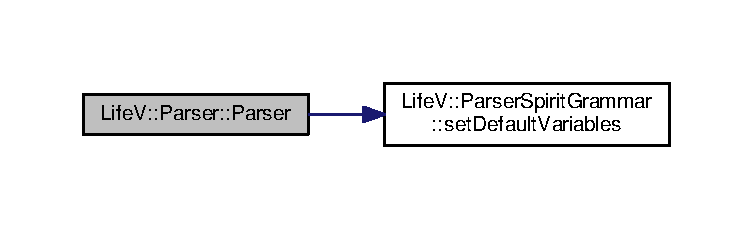
\includegraphics[width=350pt]{classLifeV_1_1Parser_a439ecd746d503e75b6e07f2933a665dc_cgraph}
\end{center}
\end{figure}


\hypertarget{classLifeV_1_1Parser_a6acf25b7222f0c65d1414611236d1820}{\index{Life\-V\-::\-Parser@{Life\-V\-::\-Parser}!Parser@{Parser}}
\index{Parser@{Parser}!LifeV::Parser@{Life\-V\-::\-Parser}}
\subsubsection[{Parser}]{\setlength{\rightskip}{0pt plus 5cm}Life\-V\-::\-Parser\-::\-Parser (
\begin{DoxyParamCaption}
\item[{const std\-::string \&}]{string}
\end{DoxyParamCaption}
)\hspace{0.3cm}{\ttfamily [explicit]}}}\label{classLifeV_1_1Parser_a6acf25b7222f0c65d1414611236d1820}


Constructor. 


\begin{DoxyParams}{Parametri}
{\em string} & expression to parse \\
\hline
\end{DoxyParams}

\begin{DoxyCode}
60                                         :
61         M\_strings       (),
62         M\_results       (),
63         M\_calculator    (),
64         M\_evaluate      ( \textcolor{keyword}{true} )
65 \{
66 
67 \textcolor{preprocessor}{#ifdef HAVE\_LIFEV\_DEBUG}
68 \textcolor{preprocessor}{}    Debug( 5030 ) << \textcolor{stringliteral}{"Parser::Parser( string, applyRules )"}<< \textcolor{stringliteral}{"\(\backslash\)n"};
69 \textcolor{preprocessor}{#endif}
70 \textcolor{preprocessor}{}
71     M\_calculator.\hyperlink{classLifeV_1_1ParserSpiritGrammar_aa48cdca46ab32d3c1e55e656aa82e902}{setDefaultVariables}();
72     \hyperlink{classLifeV_1_1Parser_ac05769e836a0dc95d9c020df361a5194}{setString}( \textcolor{keywordtype}{string} );
73 \}
\end{DoxyCode}


Questo è il grafo delle chiamate per questa funzione\-:
\nopagebreak
\begin{figure}[H]
\begin{center}
\leavevmode
\includegraphics[width=350pt]{classLifeV_1_1Parser_a6acf25b7222f0c65d1414611236d1820_cgraph}
\end{center}
\end{figure}


\hypertarget{classLifeV_1_1Parser_a0f7c4d10928fd2139e76baf44996b610}{\index{Life\-V\-::\-Parser@{Life\-V\-::\-Parser}!Parser@{Parser}}
\index{Parser@{Parser}!LifeV::Parser@{Life\-V\-::\-Parser}}
\subsubsection[{Parser}]{\setlength{\rightskip}{0pt plus 5cm}Life\-V\-::\-Parser\-::\-Parser (
\begin{DoxyParamCaption}
\item[{const {\bf Parser} \&}]{parser}
\end{DoxyParamCaption}
)\hspace{0.3cm}{\ttfamily [explicit]}}}\label{classLifeV_1_1Parser_a0f7c4d10928fd2139e76baf44996b610}


Copy constructor. 


\begin{DoxyParams}{Parametri}
{\em parser} & \hyperlink{classLifeV_1_1Parser}{Parser} \\
\hline
\end{DoxyParams}

\begin{DoxyCode}
75                                      :
76         M\_strings       ( parser.M\_strings ),
77         M\_results       ( parser.M\_results ),
78         M\_calculator    ( parser.M\_calculator ),
79         M\_evaluate      ( parser.M\_evaluate )
80 \{
81 \}
\end{DoxyCode}
\hypertarget{classLifeV_1_1Parser_a34d16f77f23cf33b3bc3f8293ed0e2ed}{\index{Life\-V\-::\-Parser@{Life\-V\-::\-Parser}!$\sim$\-Parser@{$\sim$\-Parser}}
\index{$\sim$\-Parser@{$\sim$\-Parser}!LifeV::Parser@{Life\-V\-::\-Parser}}
\subsubsection[{$\sim$\-Parser}]{\setlength{\rightskip}{0pt plus 5cm}virtual Life\-V\-::\-Parser\-::$\sim$\-Parser (
\begin{DoxyParamCaption}
{}
\end{DoxyParamCaption}
)\hspace{0.3cm}{\ttfamily [inline]}, {\ttfamily [virtual]}}}\label{classLifeV_1_1Parser_a34d16f77f23cf33b3bc3f8293ed0e2ed}


Destructor. 


\begin{DoxyCode}
89 \{\}
\end{DoxyCode}


\subsection{Documentazione delle funzioni membro}
\hypertarget{classLifeV_1_1Parser_acbc44ff1f0b0074f071ea264a95cb9e7}{\index{Life\-V\-::\-Parser@{Life\-V\-::\-Parser}!clear\-Variables@{clear\-Variables}}
\index{clear\-Variables@{clear\-Variables}!LifeV::Parser@{Life\-V\-::\-Parser}}
\subsubsection[{clear\-Variables}]{\setlength{\rightskip}{0pt plus 5cm}void Life\-V\-::\-Parser\-::clear\-Variables (
\begin{DoxyParamCaption}
{}
\end{DoxyParamCaption}
)}}\label{classLifeV_1_1Parser_acbc44ff1f0b0074f071ea264a95cb9e7}


Clear all the variables. 


\begin{DoxyCode}
161 \{
162     M\_calculator.\hyperlink{classLifeV_1_1ParserSpiritGrammar_a81b8e2abdda8a35738367f2dcfb69c75}{clearVariables}();
163     M\_evaluate = \textcolor{keyword}{true};
164 \}
\end{DoxyCode}


Questo è il grafo delle chiamate per questa funzione\-:
\nopagebreak
\begin{figure}[H]
\begin{center}
\leavevmode
\includegraphics[width=350pt]{classLifeV_1_1Parser_acbc44ff1f0b0074f071ea264a95cb9e7_cgraph}
\end{center}
\end{figure}


\hypertarget{classLifeV_1_1Parser_a37ae3af9abcf72ca8e1537ec771b523a}{\index{Life\-V\-::\-Parser@{Life\-V\-::\-Parser}!count\-Substring@{count\-Substring}}
\index{count\-Substring@{count\-Substring}!LifeV::Parser@{Life\-V\-::\-Parser}}
\subsubsection[{count\-Substring}]{\setlength{\rightskip}{0pt plus 5cm}{\bf U\-Int} Life\-V\-::\-Parser\-::count\-Substring (
\begin{DoxyParamCaption}
\item[{const std\-::string \&}]{substring}
\end{DoxyParamCaption}
)}}\label{classLifeV_1_1Parser_a37ae3af9abcf72ca8e1537ec771b523a}
Count how many times a substring is present in the string (utility for B\-C\-Interface\-Function)


\begin{DoxyParams}{Parametri}
{\em substring} & string to find \\
\hline
\end{DoxyParams}
\begin{DoxyReturn}{Restituisce}
number of substring 
\end{DoxyReturn}

\begin{DoxyCode}
141 \{
142     \hyperlink{namespaceLifeV_a4bd093cf6b0d5b57b2d89e0e90d610b7}{UInt} count( 0 );
143     std::string::size\_type position( 0 );
144 
145     \textcolor{keywordflow}{for} ( ;; )
146     \{
147         position = M\_strings.back().find( substring, position );
148 
149         \textcolor{keywordflow}{if} ( position == std::string::npos )
150             \textcolor{keywordflow}{break};
151 
152         ++count;
153         position += substring.length(); \textcolor{comment}{// start next search after this substring}
154     \}
155 
156     \textcolor{keywordflow}{return} count;
157 \}
\end{DoxyCode}


Questo è il grafo dei chiamanti di questa funzione\-:
\nopagebreak
\begin{figure}[H]
\begin{center}
\leavevmode
\includegraphics[width=350pt]{classLifeV_1_1Parser_a37ae3af9abcf72ca8e1537ec771b523a_icgraph}
\end{center}
\end{figure}


\hypertarget{classLifeV_1_1Parser_a51d84fd4ae6d420620e7beee58fad673}{\index{Life\-V\-::\-Parser@{Life\-V\-::\-Parser}!evaluate@{evaluate}}
\index{evaluate@{evaluate}!LifeV::Parser@{Life\-V\-::\-Parser}}
\subsubsection[{evaluate}]{\setlength{\rightskip}{0pt plus 5cm}const {\bf Real} \& Life\-V\-::\-Parser\-::evaluate (
\begin{DoxyParamCaption}
\item[{const {\bf I\-D} \&}]{id = {\ttfamily 0}}
\end{DoxyParamCaption}
)}}\label{classLifeV_1_1Parser_a51d84fd4ae6d420620e7beee58fad673}
Evaluate the expression 
\begin{DoxyParams}{Parametri}
{\em id} & expression index (starting from 0) \\
\hline
\end{DoxyParams}
\begin{DoxyReturn}{Restituisce}
computed value 
\end{DoxyReturn}

\begin{DoxyCode}
105 \{
106     \textcolor{keywordflow}{if} ( M\_evaluate )
107     \{
108         M\_results.clear();
109         \hyperlink{classLifeV_1_1Parser_a9491c77a9093b41468ca54b865c893ff}{stringIterator\_Type} start, end;
110 
111         \textcolor{keywordflow}{for} ( \hyperlink{namespaceLifeV_a4bd093cf6b0d5b57b2d89e0e90d610b7}{UInt} \hyperlink{god__e_8m_a8604be5925f4266ab5ccc69675329c80}{i}(0); \hyperlink{god__e_8m_a8604be5925f4266ab5ccc69675329c80}{i} < M\_strings.size(); ++\hyperlink{god__e_8m_a8604be5925f4266ab5ccc69675329c80}{i} )
112         \{
113             start = M\_strings[\hyperlink{god__e_8m_a8604be5925f4266ab5ccc69675329c80}{i}].begin();
114             end   = M\_strings[\hyperlink{god__e_8m_a8604be5925f4266ab5ccc69675329c80}{i}].end();
115 \textcolor{comment}{//#ifdef HAVE\_BOOST\_SPIRIT\_QI}
116             qi::phrase\_parse( start, end, M\_calculator, ascii::space, M\_results );
117 \textcolor{comment}{/*#else}
118 \textcolor{comment}{            std::cout << "!!! ERROR: Boost version < 1.41 !!!" << std::endl;}
119 \textcolor{comment}{            // This generate an error ---------}
120 \textcolor{comment}{            Int *a = new Int(0);}
121 \textcolor{comment}{            Int *b;}
122 \textcolor{comment}{            b = a;}
123 \textcolor{comment}{            delete a;}
124 \textcolor{comment}{            delete b;}
125 \textcolor{comment}{            // --------------------------------}
126 \textcolor{comment}{#endif*/}
127         \}
128 
129         M\_evaluate = \textcolor{keyword}{false};
130     \}
131 
132 \textcolor{preprocessor}{#ifdef HAVE\_LIFEV\_DEBUG}
133 \textcolor{preprocessor}{}    Debug( 5030 ) << \textcolor{stringliteral}{"Parser::evaluate          results[ "}<< \textcolor{keywordtype}{id} << \textcolor{stringliteral}{"]: "} << M\_results[id] << \textcolor{stringliteral}{"\(\backslash\)n"};
134 \textcolor{preprocessor}{#endif}
135 \textcolor{preprocessor}{}
136     \textcolor{keywordflow}{return} M\_results[id];
137 \}
\end{DoxyCode}


Questo è il grafo dei chiamanti di questa funzione\-:
\nopagebreak
\begin{figure}[H]
\begin{center}
\leavevmode
\includegraphics[width=350pt]{classLifeV_1_1Parser_a51d84fd4ae6d420620e7beee58fad673_icgraph}
\end{center}
\end{figure}


\hypertarget{classLifeV_1_1Parser_a257904e57f46427a5bd7c9f80e658c2d}{\index{Life\-V\-::\-Parser@{Life\-V\-::\-Parser}!operator=@{operator=}}
\index{operator=@{operator=}!LifeV::Parser@{Life\-V\-::\-Parser}}
\subsubsection[{operator=}]{\setlength{\rightskip}{0pt plus 5cm}{\bf Parser} \& Life\-V\-::\-Parser\-::operator= (
\begin{DoxyParamCaption}
\item[{const {\bf Parser} \&}]{parser}
\end{DoxyParamCaption}
)}}\label{classLifeV_1_1Parser_a257904e57f46427a5bd7c9f80e658c2d}


Operator =. 


\begin{DoxyParams}{Parametri}
{\em parser} & \hyperlink{classLifeV_1_1Parser}{Parser} \\
\hline
\end{DoxyParams}
\begin{DoxyReturn}{Restituisce}
reference to a copy of the class 
\end{DoxyReturn}

\begin{DoxyCode}
88 \{
89     \textcolor{keywordflow}{if} ( \textcolor{keyword}{this} != &parser )
90     \{
91         M\_strings    = parser.M\_strings;
92         M\_results    = parser.M\_results;
93         \textcolor{comment}{//M\_calculator = parser.M\_calculator; //NOT WORKING!!!}
94         M\_evaluate   = parser.M\_evaluate;
95     \}
96 
97     \textcolor{keywordflow}{return} *\textcolor{keyword}{this};
98 \}
\end{DoxyCode}
\hypertarget{classLifeV_1_1Parser_ac05769e836a0dc95d9c020df361a5194}{\index{Life\-V\-::\-Parser@{Life\-V\-::\-Parser}!set\-String@{set\-String}}
\index{set\-String@{set\-String}!LifeV::Parser@{Life\-V\-::\-Parser}}
\subsubsection[{set\-String}]{\setlength{\rightskip}{0pt plus 5cm}void Life\-V\-::\-Parser\-::set\-String (
\begin{DoxyParamCaption}
\item[{const std\-::string \&}]{string, }
\item[{const std\-::string \&}]{string\-Separator = {\ttfamily \char`\"{};\char`\"{}}}
\end{DoxyParamCaption}
)}}\label{classLifeV_1_1Parser_ac05769e836a0dc95d9c020df361a5194}
Set string function


\begin{DoxyParams}{Parametri}
{\em string} & Expression to evaluate \\
\hline
{\em string\-Separator} & Separator identifier (default -\/$>$ \char`\"{};\char`\"{}) \\
\hline
\end{DoxyParams}

\begin{DoxyCode}
171 \{
172 
173 \textcolor{preprocessor}{#ifdef HAVE\_LIFEV\_DEBUG}
174 \textcolor{preprocessor}{}    Debug( 5030 ) << \textcolor{stringliteral}{"Parser::setString:          strings: "} << \textcolor{keywordtype}{string} << \textcolor{stringliteral}{"\(\backslash\)n"};
175 \textcolor{preprocessor}{#endif}
176 \textcolor{preprocessor}{}
177     M\_strings.clear();
178     boost::split( M\_strings, \textcolor{keywordtype}{string}, boost::is\_any\_of( stringSeparator ) );
179 
180     \textcolor{comment}{//Remove white space to speed up the parser}
181     \textcolor{keywordflow}{for} ( \hyperlink{namespaceLifeV_a4bd093cf6b0d5b57b2d89e0e90d610b7}{UInt} \hyperlink{god__e_8m_a8604be5925f4266ab5ccc69675329c80}{i} = 0; \hyperlink{god__e_8m_a8604be5925f4266ab5ccc69675329c80}{i} < M\_strings.size(); ++\hyperlink{god__e_8m_a8604be5925f4266ab5ccc69675329c80}{i} )
182         boost::replace\_all( M\_strings[\hyperlink{god__e_8m_a8604be5925f4266ab5ccc69675329c80}{i}], \textcolor{stringliteral}{" "}, \textcolor{stringliteral}{""} );
183 
184     \textcolor{comment}{//Reserve the space for results}
185     M\_results.clear();
186     M\_results.reserve( \hyperlink{classLifeV_1_1Parser_a37ae3af9abcf72ca8e1537ec771b523a}{countSubstring}( \textcolor{stringliteral}{","} ) + 1 );
187 
188     M\_evaluate = \textcolor{keyword}{true};
189 \}
\end{DoxyCode}


Questo è il grafo delle chiamate per questa funzione\-:
\nopagebreak
\begin{figure}[H]
\begin{center}
\leavevmode
\includegraphics[width=350pt]{classLifeV_1_1Parser_ac05769e836a0dc95d9c020df361a5194_cgraph}
\end{center}
\end{figure}




Questo è il grafo dei chiamanti di questa funzione\-:
\nopagebreak
\begin{figure}[H]
\begin{center}
\leavevmode
\includegraphics[width=350pt]{classLifeV_1_1Parser_ac05769e836a0dc95d9c020df361a5194_icgraph}
\end{center}
\end{figure}


\hypertarget{classLifeV_1_1Parser_aa2b362e12b8feb60231705d499c9fbae}{\index{Life\-V\-::\-Parser@{Life\-V\-::\-Parser}!set\-Variable@{set\-Variable}}
\index{set\-Variable@{set\-Variable}!LifeV::Parser@{Life\-V\-::\-Parser}}
\subsubsection[{set\-Variable}]{\setlength{\rightskip}{0pt plus 5cm}void Life\-V\-::\-Parser\-::set\-Variable (
\begin{DoxyParamCaption}
\item[{const std\-::string \&}]{name, }
\item[{const {\bf Real} \&}]{value}
\end{DoxyParamCaption}
)}}\label{classLifeV_1_1Parser_aa2b362e12b8feb60231705d499c9fbae}
Set/replace a variable


\begin{DoxyParams}{Parametri}
{\em name} & name of the parameter \\
\hline
{\em value} & value of the parameter \\
\hline
\end{DoxyParams}

\begin{DoxyCode}
193 \{
194 
195 \textcolor{preprocessor}{#ifdef HAVE\_LIFEV\_DEBUG}
196 \textcolor{preprocessor}{}    Debug( 5030 ) << \textcolor{stringliteral}{"Parser\_Utility::SetVariable    variables["} << name << \textcolor{stringliteral}{"]: "} << value << \textcolor{stringliteral}{"\(\backslash\)n"};
197 \textcolor{preprocessor}{#endif}
198 \textcolor{preprocessor}{}
199     M\_calculator.\hyperlink{classLifeV_1_1ParserSpiritGrammar_a357a7e8d98940858ac6e05c106082e2e}{setVariable}( name, value);
200 
201     M\_evaluate = \textcolor{keyword}{true};
202 \}
\end{DoxyCode}


Questo è il grafo delle chiamate per questa funzione\-:
\nopagebreak
\begin{figure}[H]
\begin{center}
\leavevmode
\includegraphics[width=350pt]{classLifeV_1_1Parser_aa2b362e12b8feb60231705d499c9fbae_cgraph}
\end{center}
\end{figure}




Questo è il grafo dei chiamanti di questa funzione\-:
\nopagebreak
\begin{figure}[H]
\begin{center}
\leavevmode
\includegraphics[width=350pt]{classLifeV_1_1Parser_aa2b362e12b8feb60231705d499c9fbae_icgraph}
\end{center}
\end{figure}


\hypertarget{classLifeV_1_1Parser_a9fa902c13c73a3b1bc6db2b5e5c5c93d}{\index{Life\-V\-::\-Parser@{Life\-V\-::\-Parser}!variable@{variable}}
\index{variable@{variable}!LifeV::Parser@{Life\-V\-::\-Parser}}
\subsubsection[{variable}]{\setlength{\rightskip}{0pt plus 5cm}const {\bf Real} \& Life\-V\-::\-Parser\-::variable (
\begin{DoxyParamCaption}
\item[{const std\-::string \&}]{name}
\end{DoxyParamCaption}
)}}\label{classLifeV_1_1Parser_a9fa902c13c73a3b1bc6db2b5e5c5c93d}
Get variable


\begin{DoxyParams}{Parametri}
{\em name} & name of the parameter \\
\hline
\end{DoxyParams}
\begin{DoxyReturn}{Restituisce}
value of the variable 
\end{DoxyReturn}

\begin{DoxyCode}
209 \{
210 
211 \textcolor{preprocessor}{#ifdef HAVE\_LIFEV\_DEBUG}
212 \textcolor{preprocessor}{}    Debug( 5030 ) << \textcolor{stringliteral}{"Parser\_Utility::GetVariable    variables["} << name << \textcolor{stringliteral}{"]: "} << M\_calculator.
      \hyperlink{classLifeV_1_1ParserSpiritGrammar_a768e48421db190a4eba5144932ddc4f6}{variable}( name ) << \textcolor{stringliteral}{"\(\backslash\)n"};
213 \textcolor{preprocessor}{#endif}
214 \textcolor{preprocessor}{}
215     \textcolor{keywordflow}{return} M\_calculator.\hyperlink{classLifeV_1_1ParserSpiritGrammar_a768e48421db190a4eba5144932ddc4f6}{variable}( name );
216 \}
\end{DoxyCode}


Questo è il grafo delle chiamate per questa funzione\-:
\nopagebreak
\begin{figure}[H]
\begin{center}
\leavevmode
\includegraphics[width=350pt]{classLifeV_1_1Parser_a9fa902c13c73a3b1bc6db2b5e5c5c93d_cgraph}
\end{center}
\end{figure}




La documentazione per questa classe è stata generata a partire dai seguenti file\-:\begin{DoxyCompactItemize}
\item 
include/\hyperlink{Parser_8h}{Parser.\-h}\item 
src/\hyperlink{Parser_8cc}{Parser.\-cc}\end{DoxyCompactItemize}

\hypertarget{classLifeV_1_1ParserSpiritGrammar}{\section{Template per la classe Life\-V\-:\-:Parser\-Spirit\-Grammar$<$ Iterator\-Type, Results\-Type $>$}
\label{classLifeV_1_1ParserSpiritGrammar}\index{Life\-V\-::\-Parser\-Spirit\-Grammar$<$ Iterator\-Type, Results\-Type $>$@{Life\-V\-::\-Parser\-Spirit\-Grammar$<$ Iterator\-Type, Results\-Type $>$}}
}


\hyperlink{classLifeV_1_1ParserSpiritGrammar}{Parser\-Spirit\-Grammar} -\/ A string parser grammar based on {\ttfamily boost\-::spirit\-::qi}.  




{\ttfamily \#include $<$Parser\-Spirit\-Grammar.\-h$>$}



Diagramma delle classi per Life\-V\-:\-:Parser\-Spirit\-Grammar$<$ Iterator\-Type, Results\-Type $>$
\nopagebreak
\begin{figure}[H]
\begin{center}
\leavevmode
\includegraphics[width=228pt]{classLifeV_1_1ParserSpiritGrammar__inherit__graph}
\end{center}
\end{figure}


Diagramma di collaborazione per Life\-V\-:\-:Parser\-Spirit\-Grammar$<$ Iterator\-Type, Results\-Type $>$\-:
\nopagebreak
\begin{figure}[H]
\begin{center}
\leavevmode
\includegraphics[width=228pt]{classLifeV_1_1ParserSpiritGrammar__coll__graph}
\end{center}
\end{figure}
\subsection*{Tipi pubblici}
\begin{Indent}{\bf Public Types}\par
\begin{DoxyCompactItemize}
\item 
typedef Iterator\-Type \hyperlink{classLifeV_1_1ParserSpiritGrammar_aaa28e2ed8f68d686da1e0bcc5834ed3b}{iterator\-\_\-\-Type}
\item 
typedef boost\-::iterator\-\_\-range\\*
$<$ \hyperlink{classLifeV_1_1ParserSpiritGrammar_aaa28e2ed8f68d686da1e0bcc5834ed3b}{iterator\-\_\-\-Type} $>$ \hyperlink{classLifeV_1_1ParserSpiritGrammar_a8aca47ceac2876986dbc2ff9ee4d2edd}{iterator\-Range\-\_\-\-Type}
\item 
typedef Results\-Type \hyperlink{classLifeV_1_1ParserSpiritGrammar_a98dabec1a4a9a743a1d3b35e994cec7c}{results\-\_\-\-Type}
\end{DoxyCompactItemize}
\end{Indent}
\subsection*{Membri pubblici}
\begin{Indent}{\bf Constructors \& Destructor}\par
\begin{DoxyCompactItemize}
\item 
\hyperlink{classLifeV_1_1ParserSpiritGrammar_afd12d0ca36622930f0c5e574c96acaa7}{Parser\-Spirit\-Grammar} ()
\begin{DoxyCompactList}\small\item\em Constructor. \end{DoxyCompactList}\item 
\hyperlink{classLifeV_1_1ParserSpiritGrammar_a2a0d8a4396ae61a66edc4f320d9e79f5}{Parser\-Spirit\-Grammar} (const \hyperlink{classLifeV_1_1ParserSpiritGrammar}{Parser\-Spirit\-Grammar} \&spirit\-Grammar)
\begin{DoxyCompactList}\small\item\em Copy constructor. \end{DoxyCompactList}\item 
virtual \hyperlink{classLifeV_1_1ParserSpiritGrammar_a32c0629e6ee7ea37bb0b3159b0fa31ee}{$\sim$\-Parser\-Spirit\-Grammar} ()
\begin{DoxyCompactList}\small\item\em Destructor. \end{DoxyCompactList}\end{DoxyCompactItemize}
\end{Indent}
\begin{Indent}{\bf Operators}\par
\begin{DoxyCompactItemize}
\item 
\hyperlink{classLifeV_1_1ParserSpiritGrammar}{Parser\-Spirit\-Grammar} \& \hyperlink{classLifeV_1_1ParserSpiritGrammar_a6ce4fa32aacdc3bc7e4b38be901f94cf}{operator=} (const \hyperlink{classLifeV_1_1ParserSpiritGrammar}{Parser\-Spirit\-Grammar} \&spirit\-Grammar)
\begin{DoxyCompactList}\small\item\em Operator =. \end{DoxyCompactList}\end{DoxyCompactItemize}
\end{Indent}
\begin{Indent}{\bf Methods}\par
\begin{DoxyCompactItemize}
\item 
void \hyperlink{classLifeV_1_1ParserSpiritGrammar_a026a60af01b958c4f06877b40bbd19bf}{assign\-Variable} (const \hyperlink{classLifeV_1_1ParserSpiritGrammar_a8aca47ceac2876986dbc2ff9ee4d2edd}{iterator\-Range\-\_\-\-Type} \&string\-Iterator\-Range, const \hyperlink{namespaceLifeV_ad58c7402b26e5087b634b25d029c9c32}{Real} \&value)
\item 
void \hyperlink{classLifeV_1_1ParserSpiritGrammar_a81b8e2abdda8a35738367f2dcfb69c75}{clear\-Variables} ()
\begin{DoxyCompactList}\small\item\em Clear all the variables. \end{DoxyCompactList}\end{DoxyCompactItemize}
\end{Indent}
\begin{Indent}{\bf Set Methods}\par
\begin{DoxyCompactItemize}
\item 
void \hyperlink{classLifeV_1_1ParserSpiritGrammar_aa48cdca46ab32d3c1e55e656aa82e902}{set\-Default\-Variables} ()
\begin{DoxyCompactList}\small\item\em Set default variables. \end{DoxyCompactList}\item 
void \hyperlink{classLifeV_1_1ParserSpiritGrammar_a357a7e8d98940858ac6e05c106082e2e}{set\-Variable} (const std\-::string \&name, const \hyperlink{namespaceLifeV_ad58c7402b26e5087b634b25d029c9c32}{Real} \&value)
\end{DoxyCompactItemize}
\end{Indent}
\begin{Indent}{\bf Get Methods}\par
\begin{DoxyCompactItemize}
\item 
\hyperlink{namespaceLifeV_ad58c7402b26e5087b634b25d029c9c32}{Real} \& \hyperlink{classLifeV_1_1ParserSpiritGrammar_a768e48421db190a4eba5144932ddc4f6}{variable} (const std\-::string \&name)
\end{DoxyCompactItemize}
\end{Indent}


\subsection{Descrizione dettagliata}
\subsubsection*{template$<$typename Iterator\-Type = std\-::string\-::const\-\_\-iterator, typename Results\-Type = std\-::vector $<$ Real $>$$>$class Life\-V\-::\-Parser\-Spirit\-Grammar$<$ Iterator\-Type, Results\-Type $>$}

\hyperlink{classLifeV_1_1ParserSpiritGrammar}{Parser\-Spirit\-Grammar} -\/ A string parser grammar based on {\ttfamily boost\-::spirit\-::qi}. 

\begin{DoxyAuthor}{Autore}
(s) Cristiano Malossi
\end{DoxyAuthor}
{\ttfamily \hyperlink{classLifeV_1_1ParserSpiritGrammar}{Parser\-Spirit\-Grammar}} is a {\ttfamily boost\-::spirit\-::qi} based class to perform evaluation of {\ttfamily std\-::string} expressions.

{\bfseries E\-X\-A\-M\-P\-L\-E -\/ H\-O\-W T\-O U\-S\-E} Let's consider the following example\-: suppose that we have this function\-:

\mbox{[}u,v,w\mbox{]} = f(x,y,z,t)

where

u(x) = a$\ast$b$\ast$x v(x,y) = a/b$\ast$sqrt(x$^\wedge$2 + y$^\wedge$2) w(t) = b$\ast$t;

with \char`\"{}a\char`\"{} and \char`\"{}b\char`\"{} constants such that a=5.\-12345, b=9.\-999999.

To evaluate function f(x,y,z,t), we use this syntax\-:

string = \char`\"{}a=5.\-12345 ; b=9.\-999999 ; (a$\ast$b$\ast$x, a/b$\ast$sqrt(x$^\wedge$2 + y$^\wedge$2), b$\ast$t)\char`\"{}

where semicolons (\char`\"{};\char`\"{}) separate constants and commas (\char`\"{},\char`\"{}) separate output functions.

N\-O\-T\-E\-: Currently \hyperlink{classLifeV_1_1ParserSpiritGrammar}{Parser\-Spirit\-Grammar} works with the following operators\-: \begin{DoxyVerb}*  +, -, *, /, ^, sqrt(), sin(), cos(), tan(), exp(), log(), log10(), >, <.
*  \end{DoxyVerb}
 

\subsection{Documentazione delle ridefinizioni dei tipi (typedef)}
\hypertarget{classLifeV_1_1ParserSpiritGrammar_aaa28e2ed8f68d686da1e0bcc5834ed3b}{\index{Life\-V\-::\-Parser\-Spirit\-Grammar@{Life\-V\-::\-Parser\-Spirit\-Grammar}!iterator\-\_\-\-Type@{iterator\-\_\-\-Type}}
\index{iterator\-\_\-\-Type@{iterator\-\_\-\-Type}!LifeV::ParserSpiritGrammar@{Life\-V\-::\-Parser\-Spirit\-Grammar}}
\subsubsection[{iterator\-\_\-\-Type}]{\setlength{\rightskip}{0pt plus 5cm}template$<$typename Iterator\-Type = std\-::string\-::const\-\_\-iterator, typename Results\-Type = std\-::vector $<$ Real $>$$>$ typedef Iterator\-Type {\bf Life\-V\-::\-Parser\-Spirit\-Grammar}$<$ Iterator\-Type, Results\-Type $>$\-::{\bf iterator\-\_\-\-Type}}}\label{classLifeV_1_1ParserSpiritGrammar_aaa28e2ed8f68d686da1e0bcc5834ed3b}
\hypertarget{classLifeV_1_1ParserSpiritGrammar_a8aca47ceac2876986dbc2ff9ee4d2edd}{\index{Life\-V\-::\-Parser\-Spirit\-Grammar@{Life\-V\-::\-Parser\-Spirit\-Grammar}!iterator\-Range\-\_\-\-Type@{iterator\-Range\-\_\-\-Type}}
\index{iterator\-Range\-\_\-\-Type@{iterator\-Range\-\_\-\-Type}!LifeV::ParserSpiritGrammar@{Life\-V\-::\-Parser\-Spirit\-Grammar}}
\subsubsection[{iterator\-Range\-\_\-\-Type}]{\setlength{\rightskip}{0pt plus 5cm}template$<$typename Iterator\-Type = std\-::string\-::const\-\_\-iterator, typename Results\-Type = std\-::vector $<$ Real $>$$>$ typedef boost\-::iterator\-\_\-range$<$ {\bf iterator\-\_\-\-Type} $>$ {\bf Life\-V\-::\-Parser\-Spirit\-Grammar}$<$ Iterator\-Type, Results\-Type $>$\-::{\bf iterator\-Range\-\_\-\-Type}}}\label{classLifeV_1_1ParserSpiritGrammar_a8aca47ceac2876986dbc2ff9ee4d2edd}
\hypertarget{classLifeV_1_1ParserSpiritGrammar_a98dabec1a4a9a743a1d3b35e994cec7c}{\index{Life\-V\-::\-Parser\-Spirit\-Grammar@{Life\-V\-::\-Parser\-Spirit\-Grammar}!results\-\_\-\-Type@{results\-\_\-\-Type}}
\index{results\-\_\-\-Type@{results\-\_\-\-Type}!LifeV::ParserSpiritGrammar@{Life\-V\-::\-Parser\-Spirit\-Grammar}}
\subsubsection[{results\-\_\-\-Type}]{\setlength{\rightskip}{0pt plus 5cm}template$<$typename Iterator\-Type = std\-::string\-::const\-\_\-iterator, typename Results\-Type = std\-::vector $<$ Real $>$$>$ typedef Results\-Type {\bf Life\-V\-::\-Parser\-Spirit\-Grammar}$<$ Iterator\-Type, Results\-Type $>$\-::{\bf results\-\_\-\-Type}}}\label{classLifeV_1_1ParserSpiritGrammar_a98dabec1a4a9a743a1d3b35e994cec7c}


\subsection{Documentazione dei costruttori e dei distruttori}
\hypertarget{classLifeV_1_1ParserSpiritGrammar_afd12d0ca36622930f0c5e574c96acaa7}{\index{Life\-V\-::\-Parser\-Spirit\-Grammar@{Life\-V\-::\-Parser\-Spirit\-Grammar}!Parser\-Spirit\-Grammar@{Parser\-Spirit\-Grammar}}
\index{Parser\-Spirit\-Grammar@{Parser\-Spirit\-Grammar}!LifeV::ParserSpiritGrammar@{Life\-V\-::\-Parser\-Spirit\-Grammar}}
\subsubsection[{Parser\-Spirit\-Grammar}]{\setlength{\rightskip}{0pt plus 5cm}template$<$typename Iterator\-Type , typename Results\-Type $>$ {\bf Life\-V\-::\-Parser\-Spirit\-Grammar}$<$ Iterator\-Type, Results\-Type $>$\-::{\bf Parser\-Spirit\-Grammar} (
\begin{DoxyParamCaption}
{}
\end{DoxyParamCaption}
)\hspace{0.3cm}{\ttfamily [explicit]}}}\label{classLifeV_1_1ParserSpiritGrammar_afd12d0ca36622930f0c5e574c96acaa7}


Constructor. 


\begin{DoxyCode}
262                                                                       :
263         ParserSpiritGrammar::base\_type( M\_start ),
264         M\_start                               (),
265         M\_assignment                          (),
266 \textcolor{comment}{//        M\_command                             (),}
267         M\_expression                          (),
268         M\_compare                             (),
269         M\_plusMinus                           (),
270         M\_multiplyDivide                      (),
271         M\_elevate                             (),
272         M\_element                             (),
273         M\_number                              (),
274         M\_function                            (),
275         M\_group                               (),
276         M\_variable                            ()
277 \{
278     M\_start
279     =
280         (
281             M\_assignment
282 \textcolor{comment}{//        |  M\_command}
283         |  ( -qi::lit(\textcolor{charliteral}{'['}) >> M\_expression % \textcolor{charliteral}{','} >> -qi::lit(\textcolor{charliteral}{']'}) )
284         )
285         ;
286 
287     M\_assignment
288     =
289         (    qi::raw[qi::lexeme[(qi::alpha | \textcolor{charliteral}{'\_'}) >> *(qi::alnum | \textcolor{charliteral}{'\_'})]]
290         >>   qi::lit(\textcolor{charliteral}{'='})
291         >>   M\_expression
292         )              [phoenix::bind(&\hyperlink{classLifeV_1_1ParserSpiritGrammar_a026a60af01b958c4f06877b40bbd19bf}{ParserSpiritGrammar::assignVariable}
      ,\textcolor{keyword}{this}, qi::\_1, qi::\_2)]
293         ;
294     \textcolor{comment}{/*}
295 \textcolor{comment}{        M\_command}
296 \textcolor{comment}{            =  qi::lit("ShowMe")[phoenix::bind(&ParserSpiritGrammar::ShowMe, this)]}
297 \textcolor{comment}{        ;}
298 \textcolor{comment}{    */}
299 
300     M\_expression
301     =  *M\_compare                                        [qi::\_val = qi::\_1]
302        ;
303 
304     M\_compare
305     =   M\_plusMinus                                      [qi::\_val = qi::\_1]
306         >> *(
307             qi::lit(\textcolor{charliteral}{'>'}) >> M\_plusMinus                  [qi::\_val = qi::\_val > qi::\_1]
308         |   qi::lit(\textcolor{charliteral}{'<'}) >> M\_plusMinus                  [qi::\_val = qi::\_val < qi::\_1]
309         )
310         ;
311 
312     M\_plusMinus
313     =   M\_multiplyDivide                                 [qi::\_val = qi::\_1]
314         >> *(
315             qi::lit(\textcolor{charliteral}{'+'}) >> M\_multiplyDivide             [qi::\_val += qi::\_1]
316         |   qi::lit(\textcolor{charliteral}{'-'}) >> M\_multiplyDivide             [qi::\_val -= qi::\_1]
317         )
318         ;
319 
320     M\_multiplyDivide
321     =   M\_elevate                                        [qi::\_val = qi::\_1]
322         >> *(
323             qi::lit(\textcolor{charliteral}{'*'}) >> M\_elevate                    [qi::\_val *= qi::\_1]
324         |   qi::lit(\textcolor{charliteral}{'/'}) >> M\_elevate                    [qi::\_val /= qi::\_1]
325         )
326         ;
327 
328     M\_elevate
329     =
330         (
331             qi::lit(\textcolor{charliteral}{'-'}) >> M\_element                    [qi::\_val = qi::\_1]
332             >>  (
333                 qi::lit(\textcolor{charliteral}{'^'}) >> M\_element                [qi::\_val = -phoenix::bind(&
      ParserSpiritGrammar::pow, \textcolor{keyword}{this}, qi::\_val, qi::\_1)]
334             )
335             >> *(
336                 qi::lit(\textcolor{charliteral}{'^'}) >> M\_element                [qi::\_val = phoenix::bind(&
      ParserSpiritGrammar::pow, \textcolor{keyword}{this}, qi::\_val, qi::\_1)]
337             )
338         )
339         |
340         (
341             M\_element                                    [qi::\_val = qi::\_1]
342             >> *(
343                 qi::lit(\textcolor{charliteral}{'^'}) >> M\_element                [qi::\_val = phoenix::bind(&
      ParserSpiritGrammar::pow, \textcolor{keyword}{this}, qi::\_val, qi::\_1)]
344             )
345         )
346         ;
347 
348     M\_element
349     =
350         (
351             qi::lit(\textcolor{charliteral}{'-'}) >> M\_element                    [qi::\_val = -qi::\_1]
352         )
353         |
354         (
355             M\_number                                     [qi::\_val = qi::\_1]
356         |   M\_function                                   [qi::\_val = qi::\_1]
357         |   M\_variable                                   [qi::\_val = qi::\_1]
358         |   M\_group                                      [qi::\_val = qi::\_1]
359         )
360         ;
361 
362     M\_number
363     =
364         (
365             qi::double\_
366 \textcolor{comment}{//            ||   ('.' >> qi::double\_)}
367 \textcolor{comment}{//            >>   -('.' >> qi::double\_) | ('.' >> qi::double\_)}
368         )
369         ;
370 
371     M\_function
372     =
373         (
374             qi::lit(\textcolor{stringliteral}{"sin"})   >> M\_group                  [qi::\_val = phoenix::bind(&
      ParserSpiritGrammar::sin, \textcolor{keyword}{this},   qi::\_1)]
375         |   qi::lit(\textcolor{stringliteral}{"cos"})   >> M\_group                  [qi::\_val = phoenix::bind(&
      ParserSpiritGrammar::cos, \textcolor{keyword}{this},   qi::\_1)]
376         |   qi::lit(\textcolor{stringliteral}{"tan"})   >> M\_group                  [qi::\_val = phoenix::bind(&
      ParserSpiritGrammar::tan, \textcolor{keyword}{this},   qi::\_1)]
377         |   qi::lit(\textcolor{stringliteral}{"sqrt"})  >> M\_group                  [qi::\_val = phoenix::bind(&
      ParserSpiritGrammar::sqrt, \textcolor{keyword}{this},  qi::\_1)]
378         |   qi::lit(\textcolor{stringliteral}{"exp"})   >> M\_group                  [qi::\_val = phoenix::bind(&
      ParserSpiritGrammar::exp, \textcolor{keyword}{this},   qi::\_1)]
379         |   qi::lit(\textcolor{stringliteral}{"log"})   >> M\_group                  [qi::\_val = phoenix::bind(&
      ParserSpiritGrammar::log, \textcolor{keyword}{this},   qi::\_1)]
380         |   qi::lit(\textcolor{stringliteral}{"log10"}) >> M\_group                  [qi::\_val = phoenix::bind(&
      ParserSpiritGrammar::log10, \textcolor{keyword}{this}, qi::\_1)]
381         )
382         ;
383 
384     M\_group
385     =
386         (
387             \textcolor{charliteral}{'('}
388         >>  M\_expression                                 [qi::\_val = qi::\_1]
389         >>  \textcolor{charliteral}{')'}
390         )
391         ;
392 \}
\end{DoxyCode}


Questo è il grafo delle chiamate per questa funzione\-:
\nopagebreak
\begin{figure}[H]
\begin{center}
\leavevmode
\includegraphics[width=350pt]{classLifeV_1_1ParserSpiritGrammar_afd12d0ca36622930f0c5e574c96acaa7_cgraph}
\end{center}
\end{figure}


\hypertarget{classLifeV_1_1ParserSpiritGrammar_a2a0d8a4396ae61a66edc4f320d9e79f5}{\index{Life\-V\-::\-Parser\-Spirit\-Grammar@{Life\-V\-::\-Parser\-Spirit\-Grammar}!Parser\-Spirit\-Grammar@{Parser\-Spirit\-Grammar}}
\index{Parser\-Spirit\-Grammar@{Parser\-Spirit\-Grammar}!LifeV::ParserSpiritGrammar@{Life\-V\-::\-Parser\-Spirit\-Grammar}}
\subsubsection[{Parser\-Spirit\-Grammar}]{\setlength{\rightskip}{0pt plus 5cm}template$<$typename Iterator\-Type , typename Results\-Type $>$ {\bf Life\-V\-::\-Parser\-Spirit\-Grammar}$<$ Iterator\-Type, Results\-Type $>$\-::{\bf Parser\-Spirit\-Grammar} (
\begin{DoxyParamCaption}
\item[{const {\bf Parser\-Spirit\-Grammar}$<$ Iterator\-Type, Results\-Type $>$ \&}]{spirit\-Grammar}
\end{DoxyParamCaption}
)\hspace{0.3cm}{\ttfamily [explicit]}}}\label{classLifeV_1_1ParserSpiritGrammar_a2a0d8a4396ae61a66edc4f320d9e79f5}


Copy constructor. 


\begin{DoxyParams}{Parametri}
{\em \hyperlink{classLifeV_1_1ParserSpiritGrammar}{Parser\-Spirit\-Grammar}} & \hyperlink{classLifeV_1_1ParserSpiritGrammar}{Parser\-Spirit\-Grammar} \\
\hline
\end{DoxyParams}

\begin{DoxyCode}
395                                                                                                            
           :
396         ParserSpiritGrammar::base\_type     ( spiritGrammar.M\_start ),
397         M\_start                               ( spiritGrammar.M\_start ),
398         M\_assignment                          ( spiritGrammar.M\_assignment ),
399 \textcolor{comment}{//        M\_command                             ( spiritGrammar.M\_command ),}
400         M\_expression                          ( spiritGrammar.M\_expression ),
401         M\_compare                             ( spiritGrammar.M\_compare ),
402         M\_plusMinus                           ( spiritGrammar.M\_plusMinus ),
403         M\_multiplyDivide                      ( spiritGrammar.M\_multiplyDivide ),
404         M\_elevate                             ( spiritGrammar.M\_elevate ),
405         M\_element                             ( spiritGrammar.M\_element ),
406         M\_number                              ( spiritGrammar.M\_number ),
407         M\_function                            ( spiritGrammar.M\_function ),
408         M\_group                               ( spiritGrammar.M\_group ),
409         M\_variable                            ( spiritGrammar.M\_variable )
410 \{
411 \}
\end{DoxyCode}
\hypertarget{classLifeV_1_1ParserSpiritGrammar_a32c0629e6ee7ea37bb0b3159b0fa31ee}{\index{Life\-V\-::\-Parser\-Spirit\-Grammar@{Life\-V\-::\-Parser\-Spirit\-Grammar}!$\sim$\-Parser\-Spirit\-Grammar@{$\sim$\-Parser\-Spirit\-Grammar}}
\index{$\sim$\-Parser\-Spirit\-Grammar@{$\sim$\-Parser\-Spirit\-Grammar}!LifeV::ParserSpiritGrammar@{Life\-V\-::\-Parser\-Spirit\-Grammar}}
\subsubsection[{$\sim$\-Parser\-Spirit\-Grammar}]{\setlength{\rightskip}{0pt plus 5cm}template$<$typename Iterator\-Type = std\-::string\-::const\-\_\-iterator, typename Results\-Type = std\-::vector $<$ Real $>$$>$ virtual {\bf Life\-V\-::\-Parser\-Spirit\-Grammar}$<$ Iterator\-Type, Results\-Type $>$\-::$\sim${\bf Parser\-Spirit\-Grammar} (
\begin{DoxyParamCaption}
{}
\end{DoxyParamCaption}
)\hspace{0.3cm}{\ttfamily [inline]}, {\ttfamily [virtual]}}}\label{classLifeV_1_1ParserSpiritGrammar_a32c0629e6ee7ea37bb0b3159b0fa31ee}


Destructor. 


\begin{DoxyCode}
108 \{\}
\end{DoxyCode}


\subsection{Documentazione delle funzioni membro}
\hypertarget{classLifeV_1_1ParserSpiritGrammar_a026a60af01b958c4f06877b40bbd19bf}{\index{Life\-V\-::\-Parser\-Spirit\-Grammar@{Life\-V\-::\-Parser\-Spirit\-Grammar}!assign\-Variable@{assign\-Variable}}
\index{assign\-Variable@{assign\-Variable}!LifeV::ParserSpiritGrammar@{Life\-V\-::\-Parser\-Spirit\-Grammar}}
\subsubsection[{assign\-Variable}]{\setlength{\rightskip}{0pt plus 5cm}template$<$typename Iterator\-Type = std\-::string\-::const\-\_\-iterator, typename Results\-Type = std\-::vector $<$ Real $>$$>$ void {\bf Life\-V\-::\-Parser\-Spirit\-Grammar}$<$ Iterator\-Type, Results\-Type $>$\-::assign\-Variable (
\begin{DoxyParamCaption}
\item[{const {\bf iterator\-Range\-\_\-\-Type} \&}]{string\-Iterator\-Range, }
\item[{const {\bf Real} \&}]{value}
\end{DoxyParamCaption}
)\hspace{0.3cm}{\ttfamily [inline]}}}\label{classLifeV_1_1ParserSpiritGrammar_a026a60af01b958c4f06877b40bbd19bf}
Assign a variable using a {\ttfamily boost\-::iterator\-\_\-range} 


\begin{DoxyParams}{Parametri}
{\em string\-Iterator\-Range} & name of the parameter \\
\hline
{\em value} & value of the parameter \\
\hline
\end{DoxyParams}

\begin{DoxyCode}
134 \{ \hyperlink{classLifeV_1_1ParserSpiritGrammar_a357a7e8d98940858ac6e05c106082e2e}{setVariable}( std::string( stringIteratorRange.begin(), stringIteratorRange.end() ), value ); \}
\end{DoxyCode}


Questo è il grafo dei chiamanti di questa funzione\-:
\nopagebreak
\begin{figure}[H]
\begin{center}
\leavevmode
\includegraphics[width=350pt]{classLifeV_1_1ParserSpiritGrammar_a026a60af01b958c4f06877b40bbd19bf_icgraph}
\end{center}
\end{figure}


\hypertarget{classLifeV_1_1ParserSpiritGrammar_a81b8e2abdda8a35738367f2dcfb69c75}{\index{Life\-V\-::\-Parser\-Spirit\-Grammar@{Life\-V\-::\-Parser\-Spirit\-Grammar}!clear\-Variables@{clear\-Variables}}
\index{clear\-Variables@{clear\-Variables}!LifeV::ParserSpiritGrammar@{Life\-V\-::\-Parser\-Spirit\-Grammar}}
\subsubsection[{clear\-Variables}]{\setlength{\rightskip}{0pt plus 5cm}template$<$typename Iterator\-Type = std\-::string\-::const\-\_\-iterator, typename Results\-Type = std\-::vector $<$ Real $>$$>$ void {\bf Life\-V\-::\-Parser\-Spirit\-Grammar}$<$ Iterator\-Type, Results\-Type $>$\-::clear\-Variables (
\begin{DoxyParamCaption}
{}
\end{DoxyParamCaption}
)\hspace{0.3cm}{\ttfamily [inline]}}}\label{classLifeV_1_1ParserSpiritGrammar_a81b8e2abdda8a35738367f2dcfb69c75}


Clear all the variables. 


\begin{DoxyCode}
137 \{ M\_variable.clear(); \}
\end{DoxyCode}


Questo è il grafo dei chiamanti di questa funzione\-:
\nopagebreak
\begin{figure}[H]
\begin{center}
\leavevmode
\includegraphics[width=350pt]{classLifeV_1_1ParserSpiritGrammar_a81b8e2abdda8a35738367f2dcfb69c75_icgraph}
\end{center}
\end{figure}


\hypertarget{classLifeV_1_1ParserSpiritGrammar_a6ce4fa32aacdc3bc7e4b38be901f94cf}{\index{Life\-V\-::\-Parser\-Spirit\-Grammar@{Life\-V\-::\-Parser\-Spirit\-Grammar}!operator=@{operator=}}
\index{operator=@{operator=}!LifeV::ParserSpiritGrammar@{Life\-V\-::\-Parser\-Spirit\-Grammar}}
\subsubsection[{operator=}]{\setlength{\rightskip}{0pt plus 5cm}template$<$typename Iterator\-Type , typename Results\-Type $>$ {\bf Parser\-Spirit\-Grammar}$<$ Iterator\-Type, Results\-Type $>$ \& {\bf Life\-V\-::\-Parser\-Spirit\-Grammar}$<$ Iterator\-Type, Results\-Type $>$\-::operator= (
\begin{DoxyParamCaption}
\item[{const {\bf Parser\-Spirit\-Grammar}$<$ Iterator\-Type, Results\-Type $>$ \&}]{spirit\-Grammar}
\end{DoxyParamCaption}
)}}\label{classLifeV_1_1ParserSpiritGrammar_a6ce4fa32aacdc3bc7e4b38be901f94cf}


Operator =. 


\begin{DoxyParams}{Parametri}
{\em Spirit\-Grammar} & \hyperlink{classLifeV_1_1ParserSpiritGrammar}{Parser\-Spirit\-Grammar} \\
\hline
\end{DoxyParams}
\begin{DoxyReturn}{Restituisce}
reference to a copy of the class 
\end{DoxyReturn}

\begin{DoxyCode}
419 \{
420     \textcolor{keywordflow}{if} ( \textcolor{keyword}{this} != &spiritGrammar )
421     \{
422         ParserSpiritGrammar::base\_type::operator=( spiritGrammar.M\_start );
423 \textcolor{comment}{//        ParserSpiritGrammar< IteratorType, ResultsType >::operator=( spiritGrammar );}
424         M\_start                               = spiritGrammar.M\_start;
425         M\_assignment                          = spiritGrammar.M\_assignment;
426 \textcolor{comment}{//        M\_command                             = spiritGrammar.M\_command;}
427         M\_expression                          = spiritGrammar.M\_expression;
428         M\_compare                             = spiritGrammar.M\_compare;
429         M\_plusMinus                           = spiritGrammar.M\_plusMinus;
430         M\_multiplyDivide                      = spiritGrammar.M\_multiplyDivide;
431         M\_elevate                             = spiritGrammar.M\_elevate;
432         M\_element                             = spiritGrammar.M\_element;
433         M\_number                              = spiritGrammar.M\_number;
434         M\_function                            = spiritGrammar.M\_function;
435         M\_group                               = spiritGrammar.M\_group;
436         M\_variable                            = spiritGrammar.M\_variable;
437     \}
438 
439     \textcolor{keywordflow}{return} *\textcolor{keyword}{this};
440 \}
\end{DoxyCode}
\hypertarget{classLifeV_1_1ParserSpiritGrammar_aa48cdca46ab32d3c1e55e656aa82e902}{\index{Life\-V\-::\-Parser\-Spirit\-Grammar@{Life\-V\-::\-Parser\-Spirit\-Grammar}!set\-Default\-Variables@{set\-Default\-Variables}}
\index{set\-Default\-Variables@{set\-Default\-Variables}!LifeV::ParserSpiritGrammar@{Life\-V\-::\-Parser\-Spirit\-Grammar}}
\subsubsection[{set\-Default\-Variables}]{\setlength{\rightskip}{0pt plus 5cm}template$<$typename Iterator\-Type , typename Results\-Type $>$ void {\bf Life\-V\-::\-Parser\-Spirit\-Grammar}$<$ Iterator\-Type, Results\-Type $>$\-::set\-Default\-Variables (
\begin{DoxyParamCaption}
{}
\end{DoxyParamCaption}
)\hspace{0.3cm}{\ttfamily [inline]}}}\label{classLifeV_1_1ParserSpiritGrammar_aa48cdca46ab32d3c1e55e656aa82e902}


Set default variables. 


\begin{DoxyCode}
448 \{
449     M\_variable.add( \textcolor{stringliteral}{"pi"} , M\_PI );
450     M\_variable.add( \textcolor{stringliteral}{"e"}, M\_E );
451 \}
\end{DoxyCode}


Questo è il grafo dei chiamanti di questa funzione\-:
\nopagebreak
\begin{figure}[H]
\begin{center}
\leavevmode
\includegraphics[width=350pt]{classLifeV_1_1ParserSpiritGrammar_aa48cdca46ab32d3c1e55e656aa82e902_icgraph}
\end{center}
\end{figure}


\hypertarget{classLifeV_1_1ParserSpiritGrammar_a357a7e8d98940858ac6e05c106082e2e}{\index{Life\-V\-::\-Parser\-Spirit\-Grammar@{Life\-V\-::\-Parser\-Spirit\-Grammar}!set\-Variable@{set\-Variable}}
\index{set\-Variable@{set\-Variable}!LifeV::ParserSpiritGrammar@{Life\-V\-::\-Parser\-Spirit\-Grammar}}
\subsubsection[{set\-Variable}]{\setlength{\rightskip}{0pt plus 5cm}template$<$typename Iterator\-Type , typename Results\-Type $>$ void {\bf Life\-V\-::\-Parser\-Spirit\-Grammar}$<$ Iterator\-Type, Results\-Type $>$\-::set\-Variable (
\begin{DoxyParamCaption}
\item[{const std\-::string \&}]{name, }
\item[{const {\bf Real} \&}]{value}
\end{DoxyParamCaption}
)\hspace{0.3cm}{\ttfamily [inline]}}}\label{classLifeV_1_1ParserSpiritGrammar_a357a7e8d98940858ac6e05c106082e2e}
Set/replace a variable


\begin{DoxyParams}{Parametri}
{\em name} & name of the parameter \\
\hline
{\em value} & value of the parameter \\
\hline
\end{DoxyParams}

\begin{DoxyCode}
456 \{
457     \hyperlink{namespaceLifeV_ad58c7402b26e5087b634b25d029c9c32}{Real} *p = M\_variable.find( name );
458     \textcolor{keywordflow}{if} ( p != 0 )
459         *p = value;
460     \textcolor{keywordflow}{else}
461         M\_variable.add( name, value );
462 \}
\end{DoxyCode}


Questo è il grafo dei chiamanti di questa funzione\-:
\nopagebreak
\begin{figure}[H]
\begin{center}
\leavevmode
\includegraphics[width=350pt]{classLifeV_1_1ParserSpiritGrammar_a357a7e8d98940858ac6e05c106082e2e_icgraph}
\end{center}
\end{figure}


\hypertarget{classLifeV_1_1ParserSpiritGrammar_a768e48421db190a4eba5144932ddc4f6}{\index{Life\-V\-::\-Parser\-Spirit\-Grammar@{Life\-V\-::\-Parser\-Spirit\-Grammar}!variable@{variable}}
\index{variable@{variable}!LifeV::ParserSpiritGrammar@{Life\-V\-::\-Parser\-Spirit\-Grammar}}
\subsubsection[{variable}]{\setlength{\rightskip}{0pt plus 5cm}template$<$typename Iterator\-Type = std\-::string\-::const\-\_\-iterator, typename Results\-Type = std\-::vector $<$ Real $>$$>$ {\bf Real}\& {\bf Life\-V\-::\-Parser\-Spirit\-Grammar}$<$ Iterator\-Type, Results\-Type $>$\-::variable (
\begin{DoxyParamCaption}
\item[{const std\-::string \&}]{name}
\end{DoxyParamCaption}
)\hspace{0.3cm}{\ttfamily [inline]}}}\label{classLifeV_1_1ParserSpiritGrammar_a768e48421db190a4eba5144932ddc4f6}
Get variable


\begin{DoxyParams}{Parametri}
{\em name} & name of the parameter \\
\hline
\end{DoxyParams}
\begin{DoxyReturn}{Restituisce}
value of the variable 
\end{DoxyReturn}

\begin{DoxyCode}
170 \{ \textcolor{keywordflow}{return} M\_variable.at( name ); \}
\end{DoxyCode}


Questo è il grafo dei chiamanti di questa funzione\-:
\nopagebreak
\begin{figure}[H]
\begin{center}
\leavevmode
\includegraphics[width=350pt]{classLifeV_1_1ParserSpiritGrammar_a768e48421db190a4eba5144932ddc4f6_icgraph}
\end{center}
\end{figure}




La documentazione per questa classe è stata generata a partire dal seguente file\-:\begin{DoxyCompactItemize}
\item 
include/\hyperlink{ParserSpiritGrammar_8h}{Parser\-Spirit\-Grammar.\-h}\end{DoxyCompactItemize}

\hypertarget{classSaturationFractured}{\section{Riferimenti per la classe Saturation\-Fractured}
\label{classSaturationFractured}\index{Saturation\-Fractured@{Saturation\-Fractured}}
}


{\ttfamily \#include $<$Saturation\-Fractured.\-h$>$}

\subsection*{Membri pubblici}
\begin{DoxyCompactItemize}
\item 
\hyperlink{classSaturationFractured_a2d080ad53569f8a8c344d690903b8d11}{Saturation\-Fractured} (const Get\-Pot \&data\-File, \hyperlink{FracturesSet_8h_ac29a2a91d3af77fb459980a7db47f420}{Fractures\-Set\-Ptr\-\_\-\-Type} \&fractures, const \hyperlink{BCHandler_8h_aa175884cb453788647f17f2230a2a762}{B\-C\-Handler\-Ptr\-\_\-\-Type} \&bc\-Handler, const \hyperlink{Exporter_8h_ac9d7f94fea8b91459a536bfaa2f3910c}{Exporter\-Ptr\-\_\-\-Type} \&exporter, const std\-::string time=\char`\"{}data\-Time/\char`\"{})
\item 
void \hyperlink{classSaturationFractured_a6336137dd94d0ff95efc5967f4ab89c4}{init} ()
\begin{DoxyCompactList}\small\item\em Funzione che inizializza le matrici per costruire il sistema algebrico. \end{DoxyCompactList}\item 
void \hyperlink{classSaturationFractured_ad5271c4036ec9a4a7c58cddbb42515ec}{assembly} (const scalar\-\_\-type \&landa, const \hyperlink{Core_8h_ae3afecb4de4310d8262e9ab20cfb875b}{scalar\-Vector\-Container\-\_\-\-Type} \&\hyperlink{init_8m_aada26031cbb47e8d74da9873f5c1e3e1}{u0}, const \hyperlink{Core_8h_ae3afecb4de4310d8262e9ab20cfb875b}{scalar\-Vector\-Container\-\_\-\-Type} \&\hyperlink{quadratica_8m_a96d7a28b6a4428be15fc1017d19343fa}{flux})
\begin{DoxyCompactList}\small\item\em Funzione che assembla il sistema algebrico. \end{DoxyCompactList}\item 
void \hyperlink{classSaturationFractured_a20f1abf94a54768815c78e13a02ed209}{solve} ()
\item 
void \hyperlink{classSaturationFractured_ad7b71f3d032a3b9b52846c9277d706ec}{solve\-\_\-continuity} (const size\-\_\-type \hyperlink{god__e_8m_a8ea372f7ee3c01d11fc4b4d13b8e6a75}{f}, const \hyperlink{Core_8h_a4e75b5863535ba1dd79942de2846eff0}{scalar\-Vector\-\_\-\-Type} \&\hyperlink{init_8m_aada26031cbb47e8d74da9873f5c1e3e1}{u0}, \hyperlink{Core_8h_a4e75b5863535ba1dd79942de2846eff0}{scalar\-Vector\-\_\-\-Type} \&Flux)
\begin{DoxyCompactList}\small\item\em Funzione che risolve il problema nel caso un cui nella frattura in questione non vi siano discontinuità nel materiale. \end{DoxyCompactList}\item 
void \hyperlink{classSaturationFractured_ad1eb498b01ebc0826fd4bfe9da6b6a59}{solve\-\_\-discontinuity} (const size\-\_\-type \hyperlink{god__e_8m_a8ea372f7ee3c01d11fc4b4d13b8e6a75}{f}, const \hyperlink{Core_8h_a4e75b5863535ba1dd79942de2846eff0}{scalar\-Vector\-\_\-\-Type} \&\hyperlink{init_8m_aada26031cbb47e8d74da9873f5c1e3e1}{u0}, \hyperlink{Core_8h_a4e75b5863535ba1dd79942de2846eff0}{scalar\-Vector\-\_\-\-Type} \&Flux)
\begin{DoxyCompactList}\small\item\em Funzione che risolve il problema nel caso un cui nella frattura in questione vi siano discontinuità nel materiale. \end{DoxyCompactList}\item 
\hyperlink{FracturesSet_8h_ac29a2a91d3af77fb459980a7db47f420}{Fractures\-Set\-Ptr\-\_\-\-Type} \& \hyperlink{classSaturationFractured_afd7677569be76111c81f2fb73aef2d27}{get\-\_\-\-Fracture} ()
\item 
scalar\-\_\-type \hyperlink{classSaturationFractured_a77ac2375f36964b0e99457a900df48cf}{get\-Final\-Time} () const 
\end{DoxyCompactItemize}


\subsection{Documentazione dei costruttori e dei distruttori}
\hypertarget{classSaturationFractured_a2d080ad53569f8a8c344d690903b8d11}{\index{Saturation\-Fractured@{Saturation\-Fractured}!Saturation\-Fractured@{Saturation\-Fractured}}
\index{Saturation\-Fractured@{Saturation\-Fractured}!SaturationFractured@{Saturation\-Fractured}}
\subsubsection[{Saturation\-Fractured}]{\setlength{\rightskip}{0pt plus 5cm}Saturation\-Fractured\-::\-Saturation\-Fractured (
\begin{DoxyParamCaption}
\item[{const Get\-Pot \&}]{data\-File, }
\item[{{\bf Fractures\-Set\-Ptr\-\_\-\-Type} \&}]{fractures, }
\item[{const {\bf B\-C\-Handler\-Ptr\-\_\-\-Type} \&}]{bc\-Handler, }
\item[{const {\bf Exporter\-Ptr\-\_\-\-Type} \&}]{exporter, }
\item[{const std\-::string}]{time = {\ttfamily \char`\"{}dataTime/\char`\"{}}}
\end{DoxyParamCaption}
)}}\label{classSaturationFractured_a2d080ad53569f8a8c344d690903b8d11}

\begin{DoxyCode}
14                                                                 :
15                                           M\_section ( time ),
16                                           M\_fractures( fractures ),
17                                           M\_bcHandler( bcHandler ),
18                                           M\_exporter ( exporter ),
19                                           M\_t ( dataFile ( ( M\_section + \textcolor{stringliteral}{"endTime"} ).data (), 1. ) ),
20                                           M\_fractureSaturation ( M\_fractures->getNumberFractures() )
21 \{
22 \}
\end{DoxyCode}


\subsection{Documentazione delle funzioni membro}
\hypertarget{classSaturationFractured_ad5271c4036ec9a4a7c58cddbb42515ec}{\index{Saturation\-Fractured@{Saturation\-Fractured}!assembly@{assembly}}
\index{assembly@{assembly}!SaturationFractured@{Saturation\-Fractured}}
\subsubsection[{assembly}]{\setlength{\rightskip}{0pt plus 5cm}void Saturation\-Fractured\-::assembly (
\begin{DoxyParamCaption}
\item[{const scalar\-\_\-type \&}]{landa, }
\item[{const {\bf scalar\-Vector\-Container\-\_\-\-Type} \&}]{u0, }
\item[{const {\bf scalar\-Vector\-Container\-\_\-\-Type} \&}]{flux}
\end{DoxyParamCaption}
)}}\label{classSaturationFractured_ad5271c4036ec9a4a7c58cddbb42515ec}


Funzione che assembla il sistema algebrico. 


\begin{DoxyCode}
66 \{
67     size\_type numberFracture = M\_fractures->getNumberFractures();
68 
69     size\_type fractureShift = 0;
70 
71     \hyperlink{Core_8h_a83c51913d041a5001e8683434c09857f}{sizeVector\_Type} fractureNumberDOF ( numberFracture );
72 
73     \textcolor{comment}{// numero complessivo dei gradi di libertà}
74     size\_type fractureTotalNumberDOF = 0;
75 
76     \textcolor{keywordflow}{for} ( size\_type \hyperlink{god__e_8m_a68f477f9b30a6300d5af9b02eac82f35}{f} = 0; \hyperlink{god__e_8m_a68f477f9b30a6300d5af9b02eac82f35}{f} < numberFracture; \hyperlink{god__e_8m_a68f477f9b30a6300d5af9b02eac82f35}{f}++ )
77     \{
78         fractureNumberDOF [ \hyperlink{god__e_8m_a68f477f9b30a6300d5af9b02eac82f35}{f} ] = M\_fractures ->getFracture ( \hyperlink{god__e_8m_a68f477f9b30a6300d5af9b02eac82f35}{f} )->getData().getSpatialDiscretization() -
      1;
79 
80         fractureTotalNumberDOF += fractureNumberDOF [ \hyperlink{god__e_8m_a68f477f9b30a6300d5af9b02eac82f35}{f} ];
81     \}
82 
83     \textcolor{keywordflow}{for} ( size\_type \hyperlink{god__e_8m_a68f477f9b30a6300d5af9b02eac82f35}{f} = 0; \hyperlink{god__e_8m_a68f477f9b30a6300d5af9b02eac82f35}{f} < numberFracture; \hyperlink{god__e_8m_a68f477f9b30a6300d5af9b02eac82f35}{f}++ )
84     \{
85         \textcolor{comment}{// Impongo i flussi}
86         \textcolor{keywordflow}{for} ( size\_type \hyperlink{god__e_8m_a8604be5925f4266ab5ccc69675329c80}{i} = 1; \hyperlink{god__e_8m_a8604be5925f4266ab5ccc69675329c80}{i} < fractureNumberDOF [ \hyperlink{god__e_8m_a68f477f9b30a6300d5af9b02eac82f35}{f} ]; \hyperlink{god__e_8m_a8604be5925f4266ab5ccc69675329c80}{i}++ )
87         \{
88             ( *M\_globalRightHandSide ) [ \hyperlink{god__e_8m_a8604be5925f4266ab5ccc69675329c80}{i} + fractureShift ]  = \hyperlink{god__e_8m_ae060ce5868d35ef17bcb6e832da03be9}{u0} [ \hyperlink{god__e_8m_a68f477f9b30a6300d5af9b02eac82f35}{f} ][ \hyperlink{god__e_8m_a8604be5925f4266ab5ccc69675329c80}{i} ] - landa*(
      \hyperlink{confronto_8m_a96d7a28b6a4428be15fc1017d19343fa}{flux} [ \hyperlink{god__e_8m_a68f477f9b30a6300d5af9b02eac82f35}{f} ] [ \hyperlink{god__e_8m_a8604be5925f4266ab5ccc69675329c80}{i} ] - \hyperlink{confronto_8m_a96d7a28b6a4428be15fc1017d19343fa}{flux} [ \hyperlink{god__e_8m_a68f477f9b30a6300d5af9b02eac82f35}{f} ] [ \hyperlink{god__e_8m_a8604be5925f4266ab5ccc69675329c80}{i} - 1 ]);
89         \}
90 
91         scalar\_type \hyperlink{init_8m_ab6991d210d93a78cdbdf6de1889c1259}{a} = M\_fractures->getFracture ( \hyperlink{god__e_8m_a68f477f9b30a6300d5af9b02eac82f35}{f} )->getData().getA();
92         scalar\_type \hyperlink{init_8m_a21ad0bd836b90d08f4cf640b4c298e7c}{b} = M\_fractures->getFracture ( \hyperlink{god__e_8m_a68f477f9b30a6300d5af9b02eac82f35}{f} )->getData().getB();
93 
94         \textcolor{comment}{// Impongo le condizioni al contorno}
95         \textcolor{keywordflow}{if} ( M\_fractures->getFracture ( \hyperlink{god__e_8m_a68f477f9b30a6300d5af9b02eac82f35}{f} )->getData().getBc() ==\textcolor{stringliteral}{"f"})
96         \{
97             ( *M\_globalRightHandSide ) [ fractureShift ]  = M\_fractures->getFracture ( 
      \hyperlink{god__e_8m_a68f477f9b30a6300d5af9b02eac82f35}{f} )->getData().getCi( a );
98 
99             ( *M\_globalRightHandSide ) [ fractureShift + fractureNumberDOF [ \hyperlink{god__e_8m_a68f477f9b30a6300d5af9b02eac82f35}{f} ] - 1 ] = M\_fractures->
      getFracture ( \hyperlink{god__e_8m_a68f477f9b30a6300d5af9b02eac82f35}{f} )->getData().getCi( b );
100 
101         \}
102         \textcolor{keywordflow}{else} \textcolor{keywordflow}{if} ( M\_fractures->getFracture ( \hyperlink{god__e_8m_a68f477f9b30a6300d5af9b02eac82f35}{f} )->getData().getBc() ==\textcolor{stringliteral}{"p"})
103         \{
104             ( *M\_globalRightHandSide ) [ fractureShift ]  = ( *M\_globalRightHandSide ) [ fractureShift + 
      fractureNumberDOF [ \hyperlink{god__e_8m_a68f477f9b30a6300d5af9b02eac82f35}{f} ] - 2 ];
105             ( *M\_globalRightHandSide ) [ fractureShift + fractureNumberDOF [ \hyperlink{god__e_8m_a68f477f9b30a6300d5af9b02eac82f35}{f} ] - 1 ]  = (
       *M\_globalRightHandSide ) [ fractureShift + 1 ];
106         \}
107         \textcolor{keywordflow}{else}
108         \{
109             \textcolor{comment}{//std::cout << " bc non è stato impostato " << std::endl;}
110 
111             \textcolor{keywordflow}{if} ( M\_fractures->getFracture ( \hyperlink{god__e_8m_a68f477f9b30a6300d5af9b02eac82f35}{f} )->getData().feval\_scal( a, 1 ) > 0 )
112             \{
113                 ( *M\_globalRightHandSide ) [ fractureShift ]  = M\_fractures->getFracture ( 
      \hyperlink{god__e_8m_a68f477f9b30a6300d5af9b02eac82f35}{f} )->getData().getCi( a );
114 
115             \}
116             \textcolor{keywordflow}{if} ( M\_fractures->getFracture ( \hyperlink{god__e_8m_a68f477f9b30a6300d5af9b02eac82f35}{f} )->getData().feval\_scal( b, 1 ) > 0 )
117             \{
118                 ( *M\_globalRightHandSide ) [ fractureShift + fractureNumberDOF [ 
      \hyperlink{god__e_8m_a68f477f9b30a6300d5af9b02eac82f35}{f} ] - 1 ]  = M\_fractures->getFracture ( \hyperlink{god__e_8m_a68f477f9b30a6300d5af9b02eac82f35}{f} )->getData().getCi( b );
119             \}
120 
121         \}
122 
123         fractureShift += fractureNumberDOF [ \hyperlink{god__e_8m_a68f477f9b30a6300d5af9b02eac82f35}{f} ];
124 
125     \}
126 
127     size\_type NumCross = M\_fractures->getIntersections()->getNumberCross ();
128     size\_type NumBifurcation = M\_fractures->getIntersections()->getNumberBifurcation ();
129 
130 
131     \textcolor{keywordflow}{for} ( size\_type \hyperlink{god__e_8m_a8604be5925f4266ab5ccc69675329c80}{i} = 0; \hyperlink{god__e_8m_a8604be5925f4266ab5ccc69675329c80}{i} < NumBifurcation; \hyperlink{god__e_8m_a8604be5925f4266ab5ccc69675329c80}{i}++ )
132     \{
133         \textcolor{comment}{/*}
134 \textcolor{comment}{         * devo eliminare la riga corrispondente della riga e l'elemento corrispondente del termine noto
       per ogni frattura}
135 \textcolor{comment}{         */}
136     \}
137 
138     \textcolor{keywordflow}{return};
139 
140 \}\textcolor{comment}{// assembly}
\end{DoxyCode}


Questo è il grafo delle chiamate per questa funzione\-:
\nopagebreak
\begin{figure}[H]
\begin{center}
\leavevmode
\includegraphics[width=248pt]{classSaturationFractured_ad5271c4036ec9a4a7c58cddbb42515ec_cgraph}
\end{center}
\end{figure}




Questo è il grafo dei chiamanti di questa funzione\-:
\nopagebreak
\begin{figure}[H]
\begin{center}
\leavevmode
\includegraphics[width=320pt]{classSaturationFractured_ad5271c4036ec9a4a7c58cddbb42515ec_icgraph}
\end{center}
\end{figure}


\hypertarget{classSaturationFractured_afd7677569be76111c81f2fb73aef2d27}{\index{Saturation\-Fractured@{Saturation\-Fractured}!get\-\_\-\-Fracture@{get\-\_\-\-Fracture}}
\index{get\-\_\-\-Fracture@{get\-\_\-\-Fracture}!SaturationFractured@{Saturation\-Fractured}}
\subsubsection[{get\-\_\-\-Fracture}]{\setlength{\rightskip}{0pt plus 5cm}{\bf Fractures\-Set\-Ptr\-\_\-\-Type}\& Saturation\-Fractured\-::get\-\_\-\-Fracture (
\begin{DoxyParamCaption}
{}
\end{DoxyParamCaption}
)\hspace{0.3cm}{\ttfamily [inline]}}}\label{classSaturationFractured_afd7677569be76111c81f2fb73aef2d27}

\begin{DoxyCode}
67     \{
68         \textcolor{keywordflow}{return} M\_fractures;
69     \}
\end{DoxyCode}
\hypertarget{classSaturationFractured_a77ac2375f36964b0e99457a900df48cf}{\index{Saturation\-Fractured@{Saturation\-Fractured}!get\-Final\-Time@{get\-Final\-Time}}
\index{get\-Final\-Time@{get\-Final\-Time}!SaturationFractured@{Saturation\-Fractured}}
\subsubsection[{get\-Final\-Time}]{\setlength{\rightskip}{0pt plus 5cm}scalar\-\_\-type Saturation\-Fractured\-::get\-Final\-Time (
\begin{DoxyParamCaption}
{}
\end{DoxyParamCaption}
) const\hspace{0.3cm}{\ttfamily [inline]}}}\label{classSaturationFractured_a77ac2375f36964b0e99457a900df48cf}

\begin{DoxyCode}
72     \{
73         \textcolor{keywordflow}{return} M\_t;
74     \}
\end{DoxyCode}
\hypertarget{classSaturationFractured_a6336137dd94d0ff95efc5967f4ab89c4}{\index{Saturation\-Fractured@{Saturation\-Fractured}!init@{init}}
\index{init@{init}!SaturationFractured@{Saturation\-Fractured}}
\subsubsection[{init}]{\setlength{\rightskip}{0pt plus 5cm}void Saturation\-Fractured\-::init (
\begin{DoxyParamCaption}
{}
\end{DoxyParamCaption}
)}}\label{classSaturationFractured_a6336137dd94d0ff95efc5967f4ab89c4}


Funzione che inizializza le matrici per costruire il sistema algebrico. 


\begin{DoxyCode}
25 \{
26     size\_type numberFracture = M\_fractures->getNumberFractures();
27 
28     \hyperlink{Core_8h_a83c51913d041a5001e8683434c09857f}{sizeVector\_Type} fractureNumberDOF ( numberFracture );
29 
30     \textcolor{comment}{// numero complessivo dei gradi di libertà}
31     size\_type fractureTotalNumberDOF = 0;
32 
33     \textcolor{keywordflow}{for} ( size\_type \hyperlink{god__e_8m_a68f477f9b30a6300d5af9b02eac82f35}{f} = 0; \hyperlink{god__e_8m_a68f477f9b30a6300d5af9b02eac82f35}{f} < numberFracture; \hyperlink{god__e_8m_a68f477f9b30a6300d5af9b02eac82f35}{f}++ )
34     \{
35         fractureNumberDOF [ \hyperlink{god__e_8m_a68f477f9b30a6300d5af9b02eac82f35}{f} ] = M\_fractures ->getFracture ( \hyperlink{god__e_8m_a68f477f9b30a6300d5af9b02eac82f35}{f} )->getData().getSpatialDiscretization() -
       1;
36 
37         fractureTotalNumberDOF += fractureNumberDOF [ \hyperlink{god__e_8m_a68f477f9b30a6300d5af9b02eac82f35}{f} ];
38     \}
39 
40     \textcolor{comment}{// Inizializziamo tutte le matrici a blocchi, la matrice globale e il termine di destra per il sistema
       e il vettore delle soluzioni}
41 
42     \textcolor{comment}{// Allochiamo la matrice globale del sistema:  M\_darcyGlobalMatrix}
43     M\_globalMatrix.reset( \textcolor{keyword}{new} \hyperlink{Core_8h_afba9f623673e2ae32054015bdb5500f9}{sparseMatrix\_Type}( fractureTotalNumberDOF, 
      fractureTotalNumberDOF ));
44     gmm::clear( *M\_globalMatrix );
45 
46     \textcolor{comment}{// Allochiamo il vettore del termine noto di destra del sistema: M\_darcyGlobalRightHandSide}
47     M\_globalRightHandSide.reset( \textcolor{keyword}{new} \hyperlink{Core_8h_a4e75b5863535ba1dd79942de2846eff0}{scalarVector\_Type}( fractureTotalNumberDOF ));
48     gmm::clear( *M\_globalRightHandSide );
49 
50     \textcolor{comment}{// Allochiamo il vettore globale del termine incognito del sistema: M\_darcyVelocityAndPressure}
51     M\_saturation.reset( \textcolor{keyword}{new} \hyperlink{Core_8h_a4e75b5863535ba1dd79942de2846eff0}{scalarVector\_Type}( fractureTotalNumberDOF ));
52     gmm::clear( *M\_saturation );
53 
54     \textcolor{comment}{// Inizio a riempire la matrice globale del sistema}
55     \textcolor{keywordflow}{for} ( size\_type \hyperlink{god__e_8m_a8604be5925f4266ab5ccc69675329c80}{i} = 0; \hyperlink{god__e_8m_a8604be5925f4266ab5ccc69675329c80}{i}< fractureTotalNumberDOF; \hyperlink{god__e_8m_a8604be5925f4266ab5ccc69675329c80}{i}++ )
56     \{
57         ( *M\_globalMatrix )( \hyperlink{god__e_8m_a8604be5925f4266ab5ccc69675329c80}{i}, \hyperlink{god__e_8m_a8604be5925f4266ab5ccc69675329c80}{i} ) = 1.;
58     \}
59 
60     \textcolor{keywordflow}{return};
61 \}\textcolor{comment}{// init}
\end{DoxyCode}


Questo è il grafo delle chiamate per questa funzione\-:
\nopagebreak
\begin{figure}[H]
\begin{center}
\leavevmode
\includegraphics[width=248pt]{classSaturationFractured_a6336137dd94d0ff95efc5967f4ab89c4_cgraph}
\end{center}
\end{figure}


\hypertarget{classSaturationFractured_a20f1abf94a54768815c78e13a02ed209}{\index{Saturation\-Fractured@{Saturation\-Fractured}!solve@{solve}}
\index{solve@{solve}!SaturationFractured@{Saturation\-Fractured}}
\subsubsection[{solve}]{\setlength{\rightskip}{0pt plus 5cm}void Saturation\-Fractured\-::solve (
\begin{DoxyParamCaption}
{}
\end{DoxyParamCaption}
)}}\label{classSaturationFractured_a20f1abf94a54768815c78e13a02ed209}

\begin{DoxyCode}
145 \{
146     size\_type numberFracture = M\_fractures->getNumberFractures();
147 
148     scalar\_type \hyperlink{confronto_8m_a5e36941b3d856737e81516acd45edc50}{h} = M\_fractures->getFracture ( 0 )-> getData().getH();
149     scalar\_type \hyperlink{discontinuo_8m_ad9cea4edeb9e9d51c1305958394049ef}{cfl} = M\_fractures->getFracture ( 0 )->getData().getCfl();
150 
151     \hyperlink{Core_8h_ae3afecb4de4310d8262e9ab20cfb875b}{scalarVectorContainer\_Type} \hyperlink{god__e_8m_ae060ce5868d35ef17bcb6e832da03be9}{u0} ( numberFracture );
152 
153     \hyperlink{Core_8h_a83c51913d041a5001e8683434c09857f}{sizeVector\_Type} fractureNumberDOF ( numberFracture );
154 
155     size\_type fractureShift = 0;
156 
157     \textcolor{comment}{// numero complessivo dei gradi di libertà}
158     size\_type fractureTotalNumberDOF = 0;
159 
160     \textcolor{keywordflow}{for} ( size\_type \hyperlink{god__e_8m_a68f477f9b30a6300d5af9b02eac82f35}{f} = 0; \hyperlink{god__e_8m_a68f477f9b30a6300d5af9b02eac82f35}{f} < numberFracture; \hyperlink{god__e_8m_a68f477f9b30a6300d5af9b02eac82f35}{f}++ )
161     \{
162         fractureNumberDOF [ \hyperlink{god__e_8m_a68f477f9b30a6300d5af9b02eac82f35}{f} ] = M\_fractures ->getFracture ( \hyperlink{god__e_8m_a68f477f9b30a6300d5af9b02eac82f35}{f} )->getData().getSpatialDiscretization() -
       1;
163 
164         fractureTotalNumberDOF += fractureNumberDOF [ \hyperlink{god__e_8m_a68f477f9b30a6300d5af9b02eac82f35}{f} ];
165 
166     \}
167 
168     \textcolor{comment}{// Ricavo dt come il massimo valore che verifichi la condizione cfl per ogni frattura}
169     \textcolor{keywordflow}{for} ( size\_type \hyperlink{god__e_8m_a68f477f9b30a6300d5af9b02eac82f35}{f} = 0; \hyperlink{god__e_8m_a68f477f9b30a6300d5af9b02eac82f35}{f} < numberFracture; \hyperlink{god__e_8m_a68f477f9b30a6300d5af9b02eac82f35}{f}++ )
170     \{
171         \textcolor{keywordflow}{if} ( h > M\_fractures->getFracture ( \hyperlink{god__e_8m_a68f477f9b30a6300d5af9b02eac82f35}{f} )-> getData().getH() )
172         \{
173             h = M\_fractures->getFracture ( \hyperlink{god__e_8m_a68f477f9b30a6300d5af9b02eac82f35}{f} )-> getData().getH();
174         \}
175 
176         \textcolor{keywordflow}{if} ( cfl < M\_fractures->getFracture ( \hyperlink{god__e_8m_a68f477f9b30a6300d5af9b02eac82f35}{f} )->getData().getCfl() )
177         \{
178             cfl = M\_fractures->getFracture ( \hyperlink{god__e_8m_a68f477f9b30a6300d5af9b02eac82f35}{f} )->getData().getCfl();
179         \}
180 
181         \textcolor{comment}{// Condizione iniziale}
182         \hyperlink{god__e_8m_ae060ce5868d35ef17bcb6e832da03be9}{u0} [ \hyperlink{god__e_8m_a68f477f9b30a6300d5af9b02eac82f35}{f} ] = M\_fractures->getFracture ( \hyperlink{god__e_8m_a68f477f9b30a6300d5af9b02eac82f35}{f} )->getCi();
183 
184         M\_fractureSaturation [ \hyperlink{god__e_8m_a68f477f9b30a6300d5af9b02eac82f35}{f} ].reset(\textcolor{keyword}{new} \hyperlink{Core_8h_a4e75b5863535ba1dd79942de2846eff0}{scalarVector\_Type}( fractureNumberDOF [ 
      \hyperlink{god__e_8m_a68f477f9b30a6300d5af9b02eac82f35}{f} ], 0));
185 
186     \}
187 
188 
189     scalar\_type dt = h/\hyperlink{discontinuo_8m_ad9cea4edeb9e9d51c1305958394049ef}{cfl};
190     scalar\_type nt = ceil(M\_t/dt);
191     dt = M\_t/nt;
192     scalar\_type landa = dt/\hyperlink{confronto_8m_a5e36941b3d856737e81516acd45edc50}{h};
193 
194     std::cout << \textcolor{stringliteral}{" cfl "} << cfl << \textcolor{stringliteral}{"    dt  "} << dt << \textcolor{stringliteral}{"   nt  "} << nt << \textcolor{stringliteral}{"    landa  "} << landa << 
      std::endl;
195     \hyperlink{Core_8h_ae3afecb4de4310d8262e9ab20cfb875b}{scalarVectorContainer\_Type} \hyperlink{confronto_8m_a96d7a28b6a4428be15fc1017d19343fa}{flux}( numberFracture );
196 
197 
198     std::cout << std::endl << \textcolor{stringliteral}{"Solving problem in Omega..."} << std::flush;
199 
200     \textcolor{keywordflow}{for}( size\_type k = 0; k < nt; k++ )
201     \{
202         fractureShift = 0;
203 
204         \textcolor{keywordflow}{for} ( size\_type \hyperlink{god__e_8m_a68f477f9b30a6300d5af9b02eac82f35}{f} = 0; \hyperlink{god__e_8m_a68f477f9b30a6300d5af9b02eac82f35}{f} < numberFracture; \hyperlink{god__e_8m_a68f477f9b30a6300d5af9b02eac82f35}{f}++ )
205         \{
206 
207             \textcolor{keywordflow}{if}( M\_fractures->getFracture ( \hyperlink{god__e_8m_a68f477f9b30a6300d5af9b02eac82f35}{f} )->getData().getNumberFlux() == 1 )
208             \{
209                 std::cout << \textcolor{stringliteral}{" solve continuity "} << std::endl;
210                 \hyperlink{classSaturationFractured_ad7b71f3d032a3b9b52846c9277d706ec}{solve\_continuity} ( \hyperlink{god__e_8m_a68f477f9b30a6300d5af9b02eac82f35}{f}, \hyperlink{god__e_8m_ae060ce5868d35ef17bcb6e832da03be9}{u0} [ \hyperlink{god__e_8m_a68f477f9b30a6300d5af9b02eac82f35}{f} ], \hyperlink{confronto_8m_a96d7a28b6a4428be15fc1017d19343fa}{flux} [ f ] );
211                 std::cout << \textcolor{stringliteral}{" risolto "} << std::endl;
212             \}
213             \textcolor{keywordflow}{else}
214             \{
215                 \hyperlink{classSaturationFractured_ad1eb498b01ebc0826fd4bfe9da6b6a59}{solve\_discontinuity} ( \hyperlink{god__e_8m_a68f477f9b30a6300d5af9b02eac82f35}{f}, \hyperlink{god__e_8m_ae060ce5868d35ef17bcb6e832da03be9}{u0} [ \hyperlink{god__e_8m_a68f477f9b30a6300d5af9b02eac82f35}{f} ], \hyperlink{confronto_8m_a96d7a28b6a4428be15fc1017d19343fa}{flux} [ f ] );
216             \}
217         \}
218 
219         \hyperlink{classSaturationFractured_ad5271c4036ec9a4a7c58cddbb42515ec}{assembly} ( landa, \hyperlink{god__e_8m_ae060ce5868d35ef17bcb6e832da03be9}{u0}, \hyperlink{confronto_8m_a96d7a28b6a4428be15fc1017d19343fa}{flux} );
220 
221         \textcolor{comment}{// Solve the Saturation problem}
222         scalar\_type roundConditionNumber;
223 
224         SuperLU\_solve(*M\_globalMatrix, *M\_saturation,
225                       *M\_globalRightHandSide, roundConditionNumber);
226 
227         \textcolor{comment}{// aggiorno u0}
228         \textcolor{keywordflow}{for} (size\_type \hyperlink{god__e_8m_a68f477f9b30a6300d5af9b02eac82f35}{f} = 0; \hyperlink{god__e_8m_a68f477f9b30a6300d5af9b02eac82f35}{f} < numberFracture; \hyperlink{god__e_8m_a68f477f9b30a6300d5af9b02eac82f35}{f}++ )
229         \{
230             gmm::copy( gmm::sub\_vector( *M\_saturation, gmm::sub\_interval( fractureShift, fractureNumberDOF 
      [ \hyperlink{god__e_8m_a68f477f9b30a6300d5af9b02eac82f35}{f} ] )), \hyperlink{god__e_8m_ae060ce5868d35ef17bcb6e832da03be9}{u0} [ f ] );
231 
232             fractureShift += fractureNumberDOF [ \hyperlink{god__e_8m_a68f477f9b30a6300d5af9b02eac82f35}{f} ];
233         \}
234 
235     \}
236 
237     M\_exporter->spy(M\_globalMatrix, \textcolor{stringliteral}{"./matlab/matrice.mm"});
238 
239     fractureShift = 0;
240 
241 
242     \textcolor{comment}{// esporto la soluzione}
243     \textcolor{keywordflow}{for} ( size\_type \hyperlink{god__e_8m_a68f477f9b30a6300d5af9b02eac82f35}{f} = 0; \hyperlink{god__e_8m_a68f477f9b30a6300d5af9b02eac82f35}{f} < numberFracture; \hyperlink{god__e_8m_a68f477f9b30a6300d5af9b02eac82f35}{f}++ )
244     \{
245         gmm::copy ( gmm::sub\_vector ( *M\_saturation, gmm::sub\_interval( fractureShift, fractureNumberDOF [ 
      \hyperlink{god__e_8m_a68f477f9b30a6300d5af9b02eac82f35}{f} ] )), *( M\_fractureSaturation [ f ] ) );
246 
247         fractureShift += fractureNumberDOF [ \hyperlink{god__e_8m_a68f477f9b30a6300d5af9b02eac82f35}{f} ];
248 
249 
250         std::ostringstream ss;
251         ss << \textcolor{stringliteral}{"./matlab/risultati/saturation\_"} << f << \textcolor{stringliteral}{".txt"};
252 
253         std::string name = ss.str();
254 
255         std::ofstream exp( name );
256 
257         exp << *( M\_fractureSaturation [ \hyperlink{god__e_8m_a68f477f9b30a6300d5af9b02eac82f35}{f} ] );
258 
259     \}
260 
261     std::cout << std::endl << \textcolor{stringliteral}{" completed! "} << std::endl;
262 
263     \textcolor{keywordflow}{return};
264 
265 \}\textcolor{comment}{// solve}
\end{DoxyCode}


Questo è il grafo delle chiamate per questa funzione\-:
\nopagebreak
\begin{figure}[H]
\begin{center}
\leavevmode
\includegraphics[width=350pt]{classSaturationFractured_a20f1abf94a54768815c78e13a02ed209_cgraph}
\end{center}
\end{figure}


\hypertarget{classSaturationFractured_ad7b71f3d032a3b9b52846c9277d706ec}{\index{Saturation\-Fractured@{Saturation\-Fractured}!solve\-\_\-continuity@{solve\-\_\-continuity}}
\index{solve\-\_\-continuity@{solve\-\_\-continuity}!SaturationFractured@{Saturation\-Fractured}}
\subsubsection[{solve\-\_\-continuity}]{\setlength{\rightskip}{0pt plus 5cm}void Saturation\-Fractured\-::solve\-\_\-continuity (
\begin{DoxyParamCaption}
\item[{const size\-\_\-type}]{f, }
\item[{const {\bf scalar\-Vector\-\_\-\-Type} \&}]{u0, }
\item[{{\bf scalar\-Vector\-\_\-\-Type} \&}]{Flux}
\end{DoxyParamCaption}
)}}\label{classSaturationFractured_ad7b71f3d032a3b9b52846c9277d706ec}


Funzione che risolve il problema nel caso un cui nella frattura in questione non vi siano discontinuità nel materiale. 


\begin{DoxyCode}
269 \{
270     size\_type n = M\_fractures->getFracture ( \hyperlink{god__e_8m_a68f477f9b30a6300d5af9b02eac82f35}{f} )-> getData().getSpatialDiscretization() - 1;
271 
272     Flux.clear();
273     Flux.resize( n );
274 
275     \textcolor{comment}{// calcolo il punto di massimo o di minimo, punto in cui si annulla la derivata}
276     scalar\_type Us = \hyperlink{UsefulFunctions_8h_a41a4284c74a9bcf6e35509f5eec72a55}{max} ( M\_fractures->getFracture ( \hyperlink{god__e_8m_a68f477f9b30a6300d5af9b02eac82f35}{f} )->getData().getFlux1( 0 ), 0, 1 );
277     \textcolor{comment}{//M\_fractures->getFracture ( f )->getData().fzero( M\_fractures->getFracture ( f )->getData().getFlux1(
       0 ), 0, 1 );}
278 
279     std::cout << \textcolor{stringliteral}{"punto nullo "} << Us << std::endl;
280 
281     scalar\_type F\_Us = M\_fractures->getFracture ( \hyperlink{god__e_8m_a68f477f9b30a6300d5af9b02eac82f35}{f} )->getData().getUs();
282 
283     \textcolor{keywordflow}{for} ( size\_type \hyperlink{god__e_8m_a8604be5925f4266ab5ccc69675329c80}{i} = 0; \hyperlink{god__e_8m_a8604be5925f4266ab5ccc69675329c80}{i} < n-1; \hyperlink{god__e_8m_a8604be5925f4266ab5ccc69675329c80}{i}++)
284     \{
285 
286         \textcolor{keywordflow}{if}( F\_Us > 0 )      \textcolor{comment}{// caso A}
287         \{
288             \textcolor{keywordflow}{if} ( \hyperlink{god__e_8m_ae060ce5868d35ef17bcb6e832da03be9}{u0}[ \hyperlink{god__e_8m_a8604be5925f4266ab5ccc69675329c80}{i} ] < Us )      \textcolor{comment}{// caso 1}
289             \{
290                 \textcolor{keywordflow}{if} ( \hyperlink{god__e_8m_ae060ce5868d35ef17bcb6e832da03be9}{u0}[ \hyperlink{god__e_8m_a8604be5925f4266ab5ccc69675329c80}{i}+1 ] < Us )
291                 \{
292                     Flux[ \hyperlink{god__e_8m_a8604be5925f4266ab5ccc69675329c80}{i} ] = M\_fractures->getFracture ( \hyperlink{god__e_8m_a68f477f9b30a6300d5af9b02eac82f35}{f} )->getData().feval\_scal( 
      \hyperlink{god__e_8m_ae060ce5868d35ef17bcb6e832da03be9}{u0}[ \hyperlink{god__e_8m_a8604be5925f4266ab5ccc69675329c80}{i} ] );
293                 \}
294                 \textcolor{keywordflow}{else}
295                 \{
296                     scalar\_type F\_ul = M\_fractures->getFracture ( \hyperlink{god__e_8m_a68f477f9b30a6300d5af9b02eac82f35}{f} )->getData().feval\_scal( 
      \hyperlink{god__e_8m_ae060ce5868d35ef17bcb6e832da03be9}{u0}[ \hyperlink{god__e_8m_a8604be5925f4266ab5ccc69675329c80}{i} ] );
297                     scalar\_type F\_ur = M\_fractures->getFracture ( \hyperlink{god__e_8m_a68f477f9b30a6300d5af9b02eac82f35}{f} )->getData().feval\_scal( 
      \hyperlink{god__e_8m_ae060ce5868d35ef17bcb6e832da03be9}{u0}[ i+1 ] );
298                     Flux[ \hyperlink{god__e_8m_a8604be5925f4266ab5ccc69675329c80}{i} ] = \hyperlink{UsefulFunctions_8h_a9700932e89ccb7eeacaee21db125b0c4}{std::min}( F\_ul, F\_ur );
299                 \}
300             \}
301             \textcolor{keywordflow}{else}                    \textcolor{comment}{// caso 2}
302             \{
303                 \textcolor{keywordflow}{if} ( \hyperlink{god__e_8m_ae060ce5868d35ef17bcb6e832da03be9}{u0}[ i+1 ] < Us )
304                 \{
305                     Flux[ \hyperlink{god__e_8m_a8604be5925f4266ab5ccc69675329c80}{i} ] = F\_Us;
306                 \}
307                 \textcolor{keywordflow}{else}
308                 \{
309                     Flux[ \hyperlink{god__e_8m_a8604be5925f4266ab5ccc69675329c80}{i} ] = M\_fractures->getFracture ( \hyperlink{god__e_8m_a68f477f9b30a6300d5af9b02eac82f35}{f} )->getData().feval\_scal( 
      \hyperlink{god__e_8m_ae060ce5868d35ef17bcb6e832da03be9}{u0}[ i+1 ] );
310                 \}
311             \}
312         \}
313         \textcolor{keywordflow}{else}        \textcolor{comment}{// caso B}
314         \{
315             \textcolor{keywordflow}{if} ( \hyperlink{god__e_8m_ae060ce5868d35ef17bcb6e832da03be9}{u0}[ i ] < Us )       \textcolor{comment}{// caso 1}
316             \{
317                 \textcolor{keywordflow}{if} ( \hyperlink{god__e_8m_ae060ce5868d35ef17bcb6e832da03be9}{u0}[ i+1 ] < Us )
318                 \{
319                     Flux[ \hyperlink{god__e_8m_a8604be5925f4266ab5ccc69675329c80}{i} ] = M\_fractures->getFracture ( \hyperlink{god__e_8m_a68f477f9b30a6300d5af9b02eac82f35}{f} )->getData().feval\_scal( 
      \hyperlink{god__e_8m_ae060ce5868d35ef17bcb6e832da03be9}{u0}[ i+1 ] );
320                 \}
321                 \textcolor{keywordflow}{else}
322                 \{
323                     Flux[ \hyperlink{god__e_8m_a8604be5925f4266ab5ccc69675329c80}{i} ] = F\_Us;
324                 \}
325             \}
326             \textcolor{keywordflow}{else}                \textcolor{comment}{// caso 2}
327             \{
328                 \textcolor{keywordflow}{if} ( \hyperlink{god__e_8m_ae060ce5868d35ef17bcb6e832da03be9}{u0}[ i+1 ] < Us )
329                 \{
330                     scalar\_type F\_ul = M\_fractures->getFracture ( \hyperlink{god__e_8m_a68f477f9b30a6300d5af9b02eac82f35}{f} )->getData().feval\_scal( 
      \hyperlink{god__e_8m_ae060ce5868d35ef17bcb6e832da03be9}{u0}[ i ] );
331                     scalar\_type F\_ur = M\_fractures->getFracture ( \hyperlink{god__e_8m_a68f477f9b30a6300d5af9b02eac82f35}{f} )->getData().feval\_scal( 
      \hyperlink{god__e_8m_ae060ce5868d35ef17bcb6e832da03be9}{u0}[ i+1 ] );
332                     Flux[ \hyperlink{god__e_8m_a8604be5925f4266ab5ccc69675329c80}{i} ] = \hyperlink{UsefulFunctions_8h_a41a4284c74a9bcf6e35509f5eec72a55}{std::max}( F\_ul, F\_ur );
333                 \}
334                 \textcolor{keywordflow}{else}
335                 \{
336                     Flux[ \hyperlink{god__e_8m_a8604be5925f4266ab5ccc69675329c80}{i} ] = M\_fractures->getFracture ( \hyperlink{god__e_8m_a68f477f9b30a6300d5af9b02eac82f35}{f} )->getData().feval\_scal( 
      \hyperlink{god__e_8m_ae060ce5868d35ef17bcb6e832da03be9}{u0}[ i ] );
337                 \}
338             \}
339 
340         \}
341     \}
342 
343 
344     \textcolor{keywordflow}{return};
345 \}\textcolor{comment}{// solve\_continuity}
\end{DoxyCode}


Questo è il grafo delle chiamate per questa funzione\-:
\nopagebreak
\begin{figure}[H]
\begin{center}
\leavevmode
\includegraphics[width=350pt]{classSaturationFractured_ad7b71f3d032a3b9b52846c9277d706ec_cgraph}
\end{center}
\end{figure}




Questo è il grafo dei chiamanti di questa funzione\-:
\nopagebreak
\begin{figure}[H]
\begin{center}
\leavevmode
\includegraphics[width=320pt]{classSaturationFractured_ad7b71f3d032a3b9b52846c9277d706ec_icgraph}
\end{center}
\end{figure}


\hypertarget{classSaturationFractured_ad1eb498b01ebc0826fd4bfe9da6b6a59}{\index{Saturation\-Fractured@{Saturation\-Fractured}!solve\-\_\-discontinuity@{solve\-\_\-discontinuity}}
\index{solve\-\_\-discontinuity@{solve\-\_\-discontinuity}!SaturationFractured@{Saturation\-Fractured}}
\subsubsection[{solve\-\_\-discontinuity}]{\setlength{\rightskip}{0pt plus 5cm}void Saturation\-Fractured\-::solve\-\_\-discontinuity (
\begin{DoxyParamCaption}
\item[{const size\-\_\-type}]{f, }
\item[{const {\bf scalar\-Vector\-\_\-\-Type} \&}]{u0, }
\item[{{\bf scalar\-Vector\-\_\-\-Type} \&}]{Flux}
\end{DoxyParamCaption}
)}}\label{classSaturationFractured_ad1eb498b01ebc0826fd4bfe9da6b6a59}


Funzione che risolve il problema nel caso un cui nella frattura in questione vi siano discontinuità nel materiale. 


\begin{DoxyCode}
378 \{
379     scalar\_type x\_d = M\_fractures->getFracture ( \hyperlink{god__e_8m_a68f477f9b30a6300d5af9b02eac82f35}{f} )->getData().getXd();
380 
381     size\_type n = M\_fractures->getFracture ( \hyperlink{god__e_8m_a68f477f9b30a6300d5af9b02eac82f35}{f} )-> getData().getSpatialDiscretization()-1;
382 
383     \hyperlink{Core_8h_a4e75b5863535ba1dd79942de2846eff0}{scalarVector\_Type} fl;
384     \hyperlink{Core_8h_a4e75b5863535ba1dd79942de2846eff0}{scalarVector\_Type} \hyperlink{god__e_8m_a23a31775698fad0a58afa118f6a247bc}{fl1};
385 
386     \hyperlink{Core_8h_a4e75b5863535ba1dd79942de2846eff0}{scalarVector\_Type} gl;
387     \hyperlink{Core_8h_a4e75b5863535ba1dd79942de2846eff0}{scalarVector\_Type} gl1;
388 
389     \hyperlink{Core_8h_a4e75b5863535ba1dd79942de2846eff0}{scalarVector\_Type} F(n);
390     \hyperlink{Core_8h_a4e75b5863535ba1dd79942de2846eff0}{scalarVector\_Type} G(n);
391 
392 
393     \textcolor{comment}{// calcolo i flussi}
394     M\_fractures->getFracture ( \hyperlink{god__e_8m_a68f477f9b30a6300d5af9b02eac82f35}{f} )->getData().feval( fl, \hyperlink{god__e_8m_ae060ce5868d35ef17bcb6e832da03be9}{u0}, 1, 0 );
395     M\_fractures->getFracture ( \hyperlink{god__e_8m_a68f477f9b30a6300d5af9b02eac82f35}{f} )->getData().feval( fl1, \hyperlink{god__e_8m_ae060ce5868d35ef17bcb6e832da03be9}{u0}, 2, 0 );
396 
397     M\_fractures->getFracture ( \hyperlink{god__e_8m_a68f477f9b30a6300d5af9b02eac82f35}{f} )->getData().feval( gl, \hyperlink{god__e_8m_ae060ce5868d35ef17bcb6e832da03be9}{u0}, 1, 1 );
398     M\_fractures->getFracture ( \hyperlink{god__e_8m_a68f477f9b30a6300d5af9b02eac82f35}{f} )->getData().feval( gl1, \hyperlink{god__e_8m_ae060ce5868d35ef17bcb6e832da03be9}{u0}, 2, 1 );
399 
400     Flux.clear();
401     Flux.resize( n );
402 
403     \textcolor{keywordflow}{for} ( size\_type \hyperlink{god__e_8m_a8604be5925f4266ab5ccc69675329c80}{i} = 0; \hyperlink{god__e_8m_a8604be5925f4266ab5ccc69675329c80}{i} < n-1; \hyperlink{god__e_8m_a8604be5925f4266ab5ccc69675329c80}{i}++)
404     \{
405         \textcolor{comment}{// flusso 1}
406 
407         scalar\_type \hyperlink{god__e_8m_aaa7c61c7163e7fc36352afb33ce6c3dd}{s} = (fl[ \hyperlink{god__e_8m_a8604be5925f4266ab5ccc69675329c80}{i}+1 ] - fl[ \hyperlink{god__e_8m_a8604be5925f4266ab5ccc69675329c80}{i} ] )*(\hyperlink{god__e_8m_ae060ce5868d35ef17bcb6e832da03be9}{u0} [ \hyperlink{god__e_8m_a8604be5925f4266ab5ccc69675329c80}{i}+1 ] - \hyperlink{god__e_8m_ae060ce5868d35ef17bcb6e832da03be9}{u0} [ \hyperlink{god__e_8m_a8604be5925f4266ab5ccc69675329c80}{i} ] );
408 
409         \textcolor{keywordflow}{if} ( s >= 0)
410         \{
411             F[ \hyperlink{god__e_8m_a8604be5925f4266ab5ccc69675329c80}{i} ] = fl[ \hyperlink{god__e_8m_a8604be5925f4266ab5ccc69675329c80}{i} ];
412         \}
413         \textcolor{keywordflow}{else}
414         \{
415             F[ \hyperlink{god__e_8m_a8604be5925f4266ab5ccc69675329c80}{i} ] = fl[ i+1 ];
416         \}
417 
418         \textcolor{comment}{// entropy fix: corregge il flusso se c'è una rarefazione transonica}
419         \textcolor{keywordflow}{if} ( fl1[ i ] < 0 && fl1[ i+1] > 0)
420         \{
421             scalar\_type us;
422 
423             \textcolor{comment}{// trova il valore di u per il quale f'(u)=0}
424             \textcolor{keywordflow}{if} ( \hyperlink{god__e_8m_ae060ce5868d35ef17bcb6e832da03be9}{u0} [ i ] >= \hyperlink{god__e_8m_ae060ce5868d35ef17bcb6e832da03be9}{u0} [ i+1 ] )
425             \{
426                 us = M\_fractures->getFracture ( \hyperlink{god__e_8m_a68f477f9b30a6300d5af9b02eac82f35}{f} )->getData().fzero
427                                                     ( M\_fractures->getFracture ( 
      \hyperlink{god__e_8m_a68f477f9b30a6300d5af9b02eac82f35}{f} )->getData().getFlux1( 0 ), \hyperlink{god__e_8m_ae060ce5868d35ef17bcb6e832da03be9}{u0} [ i+1 ], \hyperlink{god__e_8m_ae060ce5868d35ef17bcb6e832da03be9}{u0} [ \hyperlink{god__e_8m_a8604be5925f4266ab5ccc69675329c80}{i} ] );
428             \}
429             \textcolor{keywordflow}{else}
430             \{
431                 us = M\_fractures->getFracture ( \hyperlink{god__e_8m_a68f477f9b30a6300d5af9b02eac82f35}{f} )->getData().fzero
432                                                     ( M\_fractures->getFracture ( 
      \hyperlink{god__e_8m_a68f477f9b30a6300d5af9b02eac82f35}{f} )->getData().getFlux1( 0 ), \hyperlink{god__e_8m_ae060ce5868d35ef17bcb6e832da03be9}{u0} [ \hyperlink{god__e_8m_a8604be5925f4266ab5ccc69675329c80}{i} ], \hyperlink{god__e_8m_ae060ce5868d35ef17bcb6e832da03be9}{u0} [ i+1 ] );
433 
434             \}
435 
436             F[ \hyperlink{god__e_8m_a8604be5925f4266ab5ccc69675329c80}{i} ] = M\_fractures->getFracture ( \hyperlink{god__e_8m_a68f477f9b30a6300d5af9b02eac82f35}{f} )->getData().feval\_scal( us );
437         \}
438 
439         \textcolor{comment}{// flusso 2}
440 
441         s = (gl[ i+1 ] - gl[ \hyperlink{god__e_8m_a8604be5925f4266ab5ccc69675329c80}{i} ] )*(\hyperlink{god__e_8m_ae060ce5868d35ef17bcb6e832da03be9}{u0} [ i+1 ] - \hyperlink{god__e_8m_ae060ce5868d35ef17bcb6e832da03be9}{u0} [ i ] );
442 
443         \textcolor{keywordflow}{if} ( s >= 0)
444         \{
445             G[ \hyperlink{god__e_8m_a8604be5925f4266ab5ccc69675329c80}{i} ] = gl[ \hyperlink{god__e_8m_a8604be5925f4266ab5ccc69675329c80}{i} ];
446         \}
447         \textcolor{keywordflow}{else}
448         \{
449             G[ \hyperlink{god__e_8m_a8604be5925f4266ab5ccc69675329c80}{i} ] = gl[ i+1 ];
450         \}
451 
452         \textcolor{comment}{// entropy fix: corregge il flusso se c'è una rarefazione transonica}
453         \textcolor{keywordflow}{if} ( gl1[ i ] < 0 && gl1[ i+1] > 0)
454         \{
455             scalar\_type us;
456 
457             \textcolor{comment}{// trova il valore di u per il quale f'(u)=0}
458             \textcolor{keywordflow}{if} ( \hyperlink{god__e_8m_ae060ce5868d35ef17bcb6e832da03be9}{u0} [ i ] >= \hyperlink{god__e_8m_ae060ce5868d35ef17bcb6e832da03be9}{u0} [ i+1 ] )
459             \{
460                 us = M\_fractures->getFracture ( \hyperlink{god__e_8m_a68f477f9b30a6300d5af9b02eac82f35}{f} )->getData().fzero
461                                                     ( M\_fractures->getFracture ( 
      \hyperlink{god__e_8m_a68f477f9b30a6300d5af9b02eac82f35}{f} )->getData().getFlux1( 1 ), \hyperlink{god__e_8m_ae060ce5868d35ef17bcb6e832da03be9}{u0} [ i+1 ], \hyperlink{god__e_8m_ae060ce5868d35ef17bcb6e832da03be9}{u0} [ \hyperlink{god__e_8m_a8604be5925f4266ab5ccc69675329c80}{i} ] );
462             \}
463             \textcolor{keywordflow}{else}
464             \{
465                 us = M\_fractures->getFracture ( \hyperlink{god__e_8m_a68f477f9b30a6300d5af9b02eac82f35}{f} )->getData().fzero
466                                                     ( M\_fractures->getFracture ( 
      \hyperlink{god__e_8m_a68f477f9b30a6300d5af9b02eac82f35}{f} )->getData().getFlux1( 1 ), \hyperlink{god__e_8m_ae060ce5868d35ef17bcb6e832da03be9}{u0} [ \hyperlink{god__e_8m_a8604be5925f4266ab5ccc69675329c80}{i} ], \hyperlink{god__e_8m_ae060ce5868d35ef17bcb6e832da03be9}{u0} [ i+1 ] );
467             \}
468 
469             G[ \hyperlink{god__e_8m_a8604be5925f4266ab5ccc69675329c80}{i} ] = M\_fractures->getFracture ( \hyperlink{god__e_8m_a68f477f9b30a6300d5af9b02eac82f35}{f} )->getData().feval\_scal( us );
470         \}
471 
472     \}
473 
474     F[ n-1 ]= fl[ n-1 ];
475     G[ n-1 ]= gl[ n-1 ];
476 
477     \textcolor{keywordflow}{for} ( size\_type i = 0; i < n-1; i++)
478     \{
479         bgeot::basic\_mesh::ref\_mesh\_pt\_ct nodes = M\_fractures->getFracture ( \hyperlink{god__e_8m_a68f477f9b30a6300d5af9b02eac82f35}{f} )->getMeshFlat().
      points\_of\_convex ( i );
480 
481         scalar\_type x1 = \hyperlink{UsefulFunctions_8h_a9700932e89ccb7eeacaee21db125b0c4}{std::min}(nodes [ 0 ] [ 0 ], nodes [ 1 ] [ 0 ]);
482         scalar\_type x2 = \hyperlink{UsefulFunctions_8h_a41a4284c74a9bcf6e35509f5eec72a55}{std::max}(nodes [ 0 ] [ 0 ], nodes [ 1 ] [ 0 ]);
483 
484         \textcolor{keywordflow}{if} ( x1 < x\_d &&  x2 != x\_d )
485         \{
486             \textcolor{comment}{//std::cout << " x1: " << x1 << "   x2: " << x2 << "    x\_d: " << x\_d << std::endl;}
487             Flux[ \hyperlink{god__e_8m_a8604be5925f4266ab5ccc69675329c80}{i} ] = F[ \hyperlink{god__e_8m_a8604be5925f4266ab5ccc69675329c80}{i} ];
488         \}
489         \textcolor{keywordflow}{else} \textcolor{keywordflow}{if} ( x1 < x\_d && x2 == x\_d ) \textcolor{comment}{//gmm::abs( x2 - x\_d) < 1.0E-4 )}
490         \{
491 
492             \textcolor{comment}{//scalar\_type s = (G[ i+1 ] - F[ i ] )*(u0 [ i+1 ] - u0 [ i ] );}
493             scalar\_type s = (G[ i+1 ] - F[ \hyperlink{god__e_8m_a8604be5925f4266ab5ccc69675329c80}{i} ] )*(gl [ i+1 ] - fl [ i ] );
494             \textcolor{comment}{/*}
495 \textcolor{comment}{            std::cout << " interfaccia " << std::endl;}
496 \textcolor{comment}{            //std::cout << " x1: " << x1 << "    x2: " << x2 << "   x\_d: " << x\_d << std::endl;}
497 \textcolor{comment}{}
498 \textcolor{comment}{            std::cout << " F[ i ]:  " << F[ i ] << "   G[i+1]: " << G[ i+1 ] << std::endl;}
499 \textcolor{comment}{            //std::cout << "uo[ i ]:  " << u0[ i ] << std::endl;}
500 \textcolor{comment}{}
501 \textcolor{comment}{            Flux[ i ] = fmin( F[ i ], G[ i+1 ] );}
502 \textcolor{comment}{            */}
503 
504             \textcolor{keywordflow}{if} ( s >= 0)
505             \{
506                 Flux[ \hyperlink{god__e_8m_a8604be5925f4266ab5ccc69675329c80}{i} ] = fl[ \hyperlink{god__e_8m_a8604be5925f4266ab5ccc69675329c80}{i} ];
507 
508             \}
509             \textcolor{keywordflow}{else}
510             \{
511                 Flux[ \hyperlink{god__e_8m_a8604be5925f4266ab5ccc69675329c80}{i} ] = gl[ i+1 ];
512             \}
513 
514 
515             \textcolor{comment}{/*}
516 \textcolor{comment}{            scalar\_type s = (gl[ i+1 ] - fl[ i ] )*(u0 [ i+1 ] - u0 [ i ] );}
517 \textcolor{comment}{}
518 \textcolor{comment}{            if ( s >= 0)}
519 \textcolor{comment}{            \{}
520 \textcolor{comment}{                Flux[ i ] = fl[ i ];}
521 \textcolor{comment}{                std::cout << "Flux[ i ]:  " << Flux[ i ] << std::endl;}
522 \textcolor{comment}{            \}}
523 \textcolor{comment}{            else}
524 \textcolor{comment}{            \{}
525 \textcolor{comment}{                Flux[ i ] = gl[ i + 1 ];}
526 \textcolor{comment}{                std::cout << "Flux[ i ]:  " << Flux[ i ] << std::endl;}
527 \textcolor{comment}{            \}}
528 \textcolor{comment}{            */}
529         \}
530         \textcolor{keywordflow}{else}
531         \{
532             Flux[ \hyperlink{god__e_8m_a8604be5925f4266ab5ccc69675329c80}{i} ] = G[ \hyperlink{god__e_8m_a8604be5925f4266ab5ccc69675329c80}{i} ];
533         \}
534 
535 
536     \}
537 
538     Flux[ n-1 ] = G[ n-1 ];
539 
540 
541 
542     \textcolor{keywordflow}{return};
543 \}\textcolor{comment}{// solve\_discontinuity}
\end{DoxyCode}


Questo è il grafo delle chiamate per questa funzione\-:
\nopagebreak
\begin{figure}[H]
\begin{center}
\leavevmode
\includegraphics[width=350pt]{classSaturationFractured_ad1eb498b01ebc0826fd4bfe9da6b6a59_cgraph}
\end{center}
\end{figure}




Questo è il grafo dei chiamanti di questa funzione\-:
\nopagebreak
\begin{figure}[H]
\begin{center}
\leavevmode
\includegraphics[width=324pt]{classSaturationFractured_ad1eb498b01ebc0826fd4bfe9da6b6a59_icgraph}
\end{center}
\end{figure}




La documentazione per questa classe è stata generata a partire dai seguenti file\-:\begin{DoxyCompactItemize}
\item 
include/\hyperlink{SaturationFractured_8h}{Saturation\-Fractured.\-h}\item 
src/\hyperlink{SaturationFractured_8cc}{Saturation\-Fractured.\-cc}\end{DoxyCompactItemize}

\chapter{Documentazione dei file}
\hypertarget{BC_8h}{\section{Riferimenti per il file include/\-B\-C.h}
\label{BC_8h}\index{include/\-B\-C.\-h@{include/\-B\-C.\-h}}
}
{\ttfamily \#include \char`\"{}Core.\-h\char`\"{}}\\*
Grafo delle dipendenze di inclusione per B\-C.\-h\-:
\nopagebreak
\begin{figure}[H]
\begin{center}
\leavevmode
\includegraphics[width=350pt]{BC_8h__incl}
\end{center}
\end{figure}
Questo grafo mostra quali altri file includono direttamente o indirettamente questo file\-:
\nopagebreak
\begin{figure}[H]
\begin{center}
\leavevmode
\includegraphics[width=350pt]{BC_8h__dep__incl}
\end{center}
\end{figure}
\subsection*{Composti}
\begin{DoxyCompactItemize}
\item 
class \hyperlink{classBC}{B\-C}
\end{DoxyCompactItemize}
\subsection*{Ridefinizioni di tipo (typedef)}
\begin{DoxyCompactItemize}
\item 
typedef \hyperlink{classBC}{B\-C} \hyperlink{BC_8h_a0fe235bbd14db4aea3ae80332cff646e}{B\-C\-\_\-\-Type}
\item 
typedef boost\-::shared\-\_\-ptr$<$ \hyperlink{classBC}{B\-C} $>$ \hyperlink{BC_8h_a088c36f945ad8f6e7e0c7c423994c6ec}{B\-C\-Ptr\-\_\-\-Type}
\item 
typedef std\-::vector$<$ \hyperlink{BC_8h_a088c36f945ad8f6e7e0c7c423994c6ec}{B\-C\-Ptr\-\_\-\-Type} $>$ \hyperlink{BC_8h_ae127263052e0676d0fe233f834ca7227}{B\-C\-Ptr\-Container\-\_\-\-Type}
\end{DoxyCompactItemize}


\subsection{Documentazione delle ridefinizioni di tipo (typedef)}
\hypertarget{BC_8h_a0fe235bbd14db4aea3ae80332cff646e}{\index{B\-C.\-h@{B\-C.\-h}!B\-C\-\_\-\-Type@{B\-C\-\_\-\-Type}}
\index{B\-C\-\_\-\-Type@{B\-C\-\_\-\-Type}!BC.h@{B\-C.\-h}}
\subsubsection[{B\-C\-\_\-\-Type}]{\setlength{\rightskip}{0pt plus 5cm}typedef {\bf B\-C} {\bf B\-C\-\_\-\-Type}}}\label{BC_8h_a0fe235bbd14db4aea3ae80332cff646e}
Classe \hyperlink{classBC}{B\-C} \hypertarget{BC_8h_a088c36f945ad8f6e7e0c7c423994c6ec}{\index{B\-C.\-h@{B\-C.\-h}!B\-C\-Ptr\-\_\-\-Type@{B\-C\-Ptr\-\_\-\-Type}}
\index{B\-C\-Ptr\-\_\-\-Type@{B\-C\-Ptr\-\_\-\-Type}!BC.h@{B\-C.\-h}}
\subsubsection[{B\-C\-Ptr\-\_\-\-Type}]{\setlength{\rightskip}{0pt plus 5cm}typedef boost\-::shared\-\_\-ptr$<${\bf B\-C}$>$ {\bf B\-C\-Ptr\-\_\-\-Type}}}\label{BC_8h_a088c36f945ad8f6e7e0c7c423994c6ec}
Puntatore alla classe \hyperlink{classBC}{B\-C} \hypertarget{BC_8h_ae127263052e0676d0fe233f834ca7227}{\index{B\-C.\-h@{B\-C.\-h}!B\-C\-Ptr\-Container\-\_\-\-Type@{B\-C\-Ptr\-Container\-\_\-\-Type}}
\index{B\-C\-Ptr\-Container\-\_\-\-Type@{B\-C\-Ptr\-Container\-\_\-\-Type}!BC.h@{B\-C.\-h}}
\subsubsection[{B\-C\-Ptr\-Container\-\_\-\-Type}]{\setlength{\rightskip}{0pt plus 5cm}typedef std\-::vector$<${\bf B\-C\-Ptr\-\_\-\-Type}$>$ {\bf B\-C\-Ptr\-Container\-\_\-\-Type}}}\label{BC_8h_ae127263052e0676d0fe233f834ca7227}
Vettore di puntatori alla classe \hyperlink{classBC}{B\-C} 
\hypertarget{BCHandler_8h}{\section{Riferimenti per il file include/\-B\-C\-Handler.h}
\label{BCHandler_8h}\index{include/\-B\-C\-Handler.\-h@{include/\-B\-C\-Handler.\-h}}
}
{\ttfamily \#include \char`\"{}Core.\-h\char`\"{}}\\*
{\ttfamily \#include \char`\"{}Fracture\-Data.\-h\char`\"{}}\\*
{\ttfamily \#include \char`\"{}B\-C.\-h\char`\"{}}\\*
Grafo delle dipendenze di inclusione per B\-C\-Handler.\-h\-:
\nopagebreak
\begin{figure}[H]
\begin{center}
\leavevmode
\includegraphics[width=350pt]{BCHandler_8h__incl}
\end{center}
\end{figure}
Questo grafo mostra quali altri file includono direttamente o indirettamente questo file\-:
\nopagebreak
\begin{figure}[H]
\begin{center}
\leavevmode
\includegraphics[width=345pt]{BCHandler_8h__dep__incl}
\end{center}
\end{figure}
\subsection*{Composti}
\begin{DoxyCompactItemize}
\item 
class \hyperlink{classBCHandler}{B\-C\-Handler}
\end{DoxyCompactItemize}
\subsection*{Ridefinizioni di tipo (typedef)}
\begin{DoxyCompactItemize}
\item 
typedef \hyperlink{classBCHandler}{B\-C\-Handler} \hyperlink{BCHandler_8h_a37cc8157d35b390c633acad42ab6da0c}{B\-C\-Handler\-\_\-\-Type}
\item 
typedef boost\-::shared\-\_\-ptr\\*
$<$ \hyperlink{BCHandler_8h_a37cc8157d35b390c633acad42ab6da0c}{B\-C\-Handler\-\_\-\-Type} $>$ \hyperlink{BCHandler_8h_aa175884cb453788647f17f2230a2a762}{B\-C\-Handler\-Ptr\-\_\-\-Type}
\end{DoxyCompactItemize}


\subsection{Documentazione delle ridefinizioni di tipo (typedef)}
\hypertarget{BCHandler_8h_a37cc8157d35b390c633acad42ab6da0c}{\index{B\-C\-Handler.\-h@{B\-C\-Handler.\-h}!B\-C\-Handler\-\_\-\-Type@{B\-C\-Handler\-\_\-\-Type}}
\index{B\-C\-Handler\-\_\-\-Type@{B\-C\-Handler\-\_\-\-Type}!BCHandler.h@{B\-C\-Handler.\-h}}
\subsubsection[{B\-C\-Handler\-\_\-\-Type}]{\setlength{\rightskip}{0pt plus 5cm}typedef {\bf B\-C\-Handler} {\bf B\-C\-Handler\-\_\-\-Type}}}\label{BCHandler_8h_a37cc8157d35b390c633acad42ab6da0c}
Classe \hyperlink{classBCHandler}{B\-C\-Handler} \hypertarget{BCHandler_8h_aa175884cb453788647f17f2230a2a762}{\index{B\-C\-Handler.\-h@{B\-C\-Handler.\-h}!B\-C\-Handler\-Ptr\-\_\-\-Type@{B\-C\-Handler\-Ptr\-\_\-\-Type}}
\index{B\-C\-Handler\-Ptr\-\_\-\-Type@{B\-C\-Handler\-Ptr\-\_\-\-Type}!BCHandler.h@{B\-C\-Handler.\-h}}
\subsubsection[{B\-C\-Handler\-Ptr\-\_\-\-Type}]{\setlength{\rightskip}{0pt plus 5cm}typedef boost\-::shared\-\_\-ptr$<${\bf B\-C\-Handler\-\_\-\-Type}$>$ {\bf B\-C\-Handler\-Ptr\-\_\-\-Type}}}\label{BCHandler_8h_aa175884cb453788647f17f2230a2a762}
Puntatore alla classe \hyperlink{classBCHandler}{B\-C\-Handler} 
\hypertarget{Core_8h}{\section{Riferimenti per il file include/\-Core.h}
\label{Core_8h}\index{include/\-Core.\-h@{include/\-Core.\-h}}
}
{\ttfamily \#include $<$getfem/getfem\-\_\-regular\-\_\-meshes.\-h$>$}\\*
{\ttfamily \#include $<$getfem/getfem\-\_\-interpolation.\-h$>$}\\*
{\ttfamily \#include $<$getfem/getfem\-\_\-config.\-h$>$}\\*
{\ttfamily \#include $<$getfem/getfem\-\_\-assembling.\-h$>$}\\*
{\ttfamily \#include $<$getfem/getfem\-\_\-import.\-h$>$}\\*
{\ttfamily \#include $<$getfem/getfem\-\_\-export.\-h$>$}\\*
{\ttfamily \#include $<$gmm/gmm.\-h$>$}\\*
{\ttfamily \#include $<$gmm/gmm\-\_\-inoutput.\-h$>$}\\*
{\ttfamily \#include $<$gmm/gmm\-\_\-\-M\-U\-M\-P\-S\-\_\-interface.\-h$>$}\\*
{\ttfamily \#include $<$gmm/gmm\-\_\-superlu\-\_\-interface.\-h$>$}\\*
{\ttfamily \#include $<$getfem/bgeot\-\_\-mesh.\-h$>$}\\*
{\ttfamily \#include $<$getfem/getfem\-\_\-mesh\-\_\-im\-\_\-level\-\_\-set.\-h$>$}\\*
{\ttfamily \#include $<$getfem/getfem\-\_\-mesh\-\_\-fem\-\_\-level\-\_\-set.\-h$>$}\\*
{\ttfamily \#include $<$string$>$}\\*
{\ttfamily \#include $<$stdio.\-h$>$}\\*
{\ttfamily \#include $<$math.\-h$>$}\\*
{\ttfamily \#include $<$fstream$>$}\\*
{\ttfamily \#include $<$sstream$>$}\\*
{\ttfamily \#include $<$cmath$>$}\\*
{\ttfamily \#include $<$assert.\-h$>$}\\*
{\ttfamily \#include $<$algorithm$>$}\\*
{\ttfamily \#include $<$getfem/getfem\-\_\-mesh\-\_\-fem\-\_\-product.\-h$>$}\\*
{\ttfamily \#include $<$getfem/getfem\-\_\-mesh\-\_\-fem\-\_\-global\-\_\-function.\-h$>$}\\*
{\ttfamily \#include \char`\"{}Get\-Pot\char`\"{}}\\*
{\ttfamily \#include $<$iostream$>$}\\*
{\ttfamily \#include $<$boost/shared\-\_\-ptr.\-hpp$>$}\\*
{\ttfamily \#include $<$iomanip$>$}\\*
{\ttfamily \#include $<$eigen3/\-Eigen/\-Dense$>$}\\*
Grafo delle dipendenze di inclusione per Core.\-h\-:
\nopagebreak
\begin{figure}[H]
\begin{center}
\leavevmode
\includegraphics[width=350pt]{Core_8h__incl}
\end{center}
\end{figure}
Questo grafo mostra quali altri file includono direttamente o indirettamente questo file\-:
\nopagebreak
\begin{figure}[H]
\begin{center}
\leavevmode
\includegraphics[width=350pt]{Core_8h__dep__incl}
\end{center}
\end{figure}
\subsection*{Namespace}
\begin{DoxyCompactItemize}
\item 
\hyperlink{namespaceLifeV}{Life\-V}
\end{DoxyCompactItemize}
\subsection*{Ridefinizioni di tipo (typedef)}
\begin{DoxyCompactItemize}
\item 
typedef gmm\-::rsvector\\*
$<$ scalar\-\_\-type $>$ \hyperlink{Core_8h_a866438488c3e9b9569ecfbb4f4739751}{sparse\-Vector\-\_\-\-Type}
\item 
typedef gmm\-::row\-\_\-matrix\\*
$<$ \hyperlink{Core_8h_a866438488c3e9b9569ecfbb4f4739751}{sparse\-Vector\-\_\-\-Type} $>$ \hyperlink{Core_8h_afba9f623673e2ae32054015bdb5500f9}{sparse\-Matrix\-\_\-\-Type}
\item 
typedef boost\-::shared\-\_\-ptr\\*
$<$ \hyperlink{Core_8h_afba9f623673e2ae32054015bdb5500f9}{sparse\-Matrix\-\_\-\-Type} $>$ \hyperlink{Core_8h_a87137a9501b38c724ac80bc955164bb7}{sparse\-Matrix\-Ptr\-\_\-\-Type}
\item 
typedef std\-::vector\\*
$<$ \hyperlink{Core_8h_afba9f623673e2ae32054015bdb5500f9}{sparse\-Matrix\-\_\-\-Type} $>$ \hyperlink{Core_8h_a95b5f3daac96e3478e8cce49aa2fe689}{sparse\-Matrix\-Container\-\_\-\-Type}
\item 
typedef std\-::vector\\*
$<$ \hyperlink{Core_8h_a87137a9501b38c724ac80bc955164bb7}{sparse\-Matrix\-Ptr\-\_\-\-Type} $>$ \hyperlink{Core_8h_a2f5e086fbce840d40be38c016488fd91}{sparse\-Matrix\-Ptr\-Container\-\_\-\-Type}
\item 
typedef std\-::vector$<$ scalar\-\_\-type $>$ \hyperlink{Core_8h_a4e75b5863535ba1dd79942de2846eff0}{scalar\-Vector\-\_\-\-Type}
\item 
typedef boost\-::shared\-\_\-ptr\\*
$<$ \hyperlink{Core_8h_a4e75b5863535ba1dd79942de2846eff0}{scalar\-Vector\-\_\-\-Type} $>$ \hyperlink{Core_8h_ab09b6fa3c23db1b8c60456f8690c44a7}{scalar\-Vector\-Ptr\-\_\-\-Type}
\item 
typedef std\-::vector\\*
$<$ \hyperlink{Core_8h_a4e75b5863535ba1dd79942de2846eff0}{scalar\-Vector\-\_\-\-Type} $>$ \hyperlink{Core_8h_ae3afecb4de4310d8262e9ab20cfb875b}{scalar\-Vector\-Container\-\_\-\-Type}
\item 
typedef boost\-::shared\-\_\-ptr\\*
$<$ \hyperlink{Core_8h_ab09b6fa3c23db1b8c60456f8690c44a7}{scalar\-Vector\-Ptr\-\_\-\-Type} $>$ \hyperlink{Core_8h_a45f913084cbd38630aa9e0d0f567ae6b}{scalar\-Vector\-Container\-Ptr\-\_\-\-Type}
\item 
typedef std\-::vector\\*
$<$ \hyperlink{Core_8h_ab09b6fa3c23db1b8c60456f8690c44a7}{scalar\-Vector\-Ptr\-\_\-\-Type} $>$ \hyperlink{Core_8h_a20f0354ac7b92989514c678f4cdfcb6b}{scalar\-Vector\-Ptr\-Container\-\_\-\-Type}
\item 
typedef std\-::vector$<$ size\-\_\-type $>$ \hyperlink{Core_8h_a83c51913d041a5001e8683434c09857f}{size\-Vector\-\_\-\-Type}
\item 
typedef boost\-::shared\-\_\-ptr\\*
$<$ \hyperlink{Core_8h_a83c51913d041a5001e8683434c09857f}{size\-Vector\-\_\-\-Type} $>$ \hyperlink{Core_8h_aae592fe3076c1985d0ad6c88172e2adf}{size\-Vector\-Ptr\-\_\-\-Type}
\item 
typedef std\-::vector\\*
$<$ \hyperlink{Core_8h_a83c51913d041a5001e8683434c09857f}{size\-Vector\-\_\-\-Type} $>$ \hyperlink{Core_8h_a80e8381d86ecb0a7f4f87ff84d1a0be5}{size\-Vector\-Container\-\_\-\-Type}
\item 
typedef std\-::vector\\*
$<$ \hyperlink{Core_8h_aae592fe3076c1985d0ad6c88172e2adf}{size\-Vector\-Ptr\-\_\-\-Type} $>$ \hyperlink{Core_8h_a19cd2e66996cb454b746a0e689857698}{size\-Vector\-Ptr\-Container\-\_\-\-Type}
\item 
typedef std\-::pair$<$ size\-\_\-type, \\*
size\-\_\-type $>$ \hyperlink{Core_8h_a6453867d4e9bd858ad9577b4a1078511}{pair\-Size\-\_\-\-Type}
\item 
typedef std\-::vector\\*
$<$ \hyperlink{Core_8h_a6453867d4e9bd858ad9577b4a1078511}{pair\-Size\-\_\-\-Type} $>$ \hyperlink{Core_8h_a25b461d8af44928b225f6d4e545a0e28}{pair\-Size\-Vector\-\_\-\-Type}
\item 
typedef std\-::vector\\*
$<$ \hyperlink{Core_8h_a25b461d8af44928b225f6d4e545a0e28}{pair\-Size\-Vector\-\_\-\-Type} $>$ \hyperlink{Core_8h_a9bc476e433f99b82a9c2b8560735c7b5}{pair\-Size\-Vector\-Container\-\_\-\-Type}
\item 
typedef std\-::vector$<$ std\-::string $>$ \hyperlink{Core_8h_abd22988c59cfec13627d6187914605c9}{string\-Container\-\_\-\-Type}
\item 
typedef getfem\-::mesh\-\_\-fem \hyperlink{Core_8h_ae7bbd1c30a789b1da88f5459e0b70ab5}{G\-F\-Mesh\-F\-E\-M\-\_\-\-Type}
\item 
typedef boost\-::shared\-\_\-ptr\\*
$<$ \hyperlink{Core_8h_ae7bbd1c30a789b1da88f5459e0b70ab5}{G\-F\-Mesh\-F\-E\-M\-\_\-\-Type} $>$ \hyperlink{Core_8h_adbcb92a7299d61d5fe4b56c6a7dab5bc}{G\-F\-Mesh\-F\-E\-M\-Ptr\-\_\-\-Type}
\item 
typedef std\-::vector\\*
$<$ \hyperlink{Core_8h_adbcb92a7299d61d5fe4b56c6a7dab5bc}{G\-F\-Mesh\-F\-E\-M\-Ptr\-\_\-\-Type} $>$ \hyperlink{Core_8h_a5a3193c466013aeb4a6eb90e5de6c8c7}{G\-F\-Mesh\-F\-E\-M\-Ptr\-Container\-\_\-\-Type}
\item 
typedef getfem\-::mesh\-\_\-level\-\_\-set \hyperlink{Core_8h_a126f7165f04db4ed0b72454469145a08}{G\-F\-Mesh\-Level\-Set\-\_\-\-Type}
\item 
typedef boost\-::shared\-\_\-ptr\\*
$<$ \hyperlink{Core_8h_a126f7165f04db4ed0b72454469145a08}{G\-F\-Mesh\-Level\-Set\-\_\-\-Type} $>$ \hyperlink{Core_8h_a1cbde831f5a62206e084de1c5de27000}{G\-F\-Mesh\-Level\-Set\-Ptr\-\_\-\-Type}
\item 
typedef std\-::vector\\*
$<$ \hyperlink{Core_8h_a1cbde831f5a62206e084de1c5de27000}{G\-F\-Mesh\-Level\-Set\-Ptr\-\_\-\-Type} $>$ \hyperlink{Core_8h_a29030a1ee2a376ae4052e25cde188912}{G\-F\-Mesh\-Level\-Set\-Ptr\-Container\-\_\-\-Type}
\item 
typedef getfem\-::level\-\_\-set \hyperlink{Core_8h_a71358a15bd3925629e26ccbb214a0133}{G\-F\-Level\-Set\-\_\-\-Type}
\item 
typedef std\-::vector\\*
$<$ \hyperlink{Core_8h_a71358a15bd3925629e26ccbb214a0133}{G\-F\-Level\-Set\-\_\-\-Type} $>$ \hyperlink{Core_8h_ad8657223c251502b6c6a7e8ce792d708}{G\-F\-Level\-Set\-Container\-\_\-\-Type}
\item 
typedef boost\-::shared\-\_\-ptr\\*
$<$ \hyperlink{Core_8h_a71358a15bd3925629e26ccbb214a0133}{G\-F\-Level\-Set\-\_\-\-Type} $>$ \hyperlink{Core_8h_a036173458a8a25c7c03f8c76d97e9580}{G\-F\-Level\-Set\-Ptr\-\_\-\-Type}
\item 
typedef std\-::vector\\*
$<$ \hyperlink{Core_8h_a036173458a8a25c7c03f8c76d97e9580}{G\-F\-Level\-Set\-Ptr\-\_\-\-Type} $>$ \hyperlink{Core_8h_a987d5dc736e8c716b3a33e3901a8c904}{G\-F\-Level\-Set\-Ptr\-Container\-\_\-\-Type}
\item 
typedef getfem\-::mesh\-\_\-im\-\_\-level\-\_\-set \hyperlink{Core_8h_ade18ba6e17965b6fdd50b3382b2a7020}{G\-F\-Integration\-Method\-Level\-Set\-\_\-\-Type}
\item 
typedef boost\-::shared\-\_\-ptr\\*
$<$ \hyperlink{Core_8h_ade18ba6e17965b6fdd50b3382b2a7020}{G\-F\-Integration\-Method\-Level\-Set\-\_\-\-Type} $>$ \hyperlink{Core_8h_a8b50cf7cff521cc16dc8ab5b1c86e622}{G\-F\-Integration\-Method\-Level\-Set\-Ptr\-\_\-\-Type}
\item 
typedef scalar\-\_\-type \hyperlink{namespaceLifeV_ad58c7402b26e5087b634b25d029c9c32}{Life\-V\-::\-Real}
\item 
typedef size\-\_\-type \hyperlink{namespaceLifeV_a4bd093cf6b0d5b57b2d89e0e90d610b7}{Life\-V\-::\-U\-Int}
\item 
typedef size\-\_\-type \hyperlink{namespaceLifeV_a7c0e64679fcd30daa5471b87a57601e9}{Life\-V\-::\-I\-D}
\item 
typedef int \hyperlink{namespaceLifeV_a86d39e8d98566ac745a6c441ed3de2dc}{Life\-V\-::\-Int}
\item 
typedef Eigen\-::\-Vector2d \hyperlink{Core_8h_a09205951ae66bf900cc5cc57e2192667}{Vector2d}
\item 
typedef Eigen\-::\-Matrix\\*
$<$ scalar\-\_\-type, 3, 2 $>$ \hyperlink{Core_8h_aee82131e398edee47a44d675ee802368}{Matrix32}
\item 
typedef Eigen\-::\-Matrix2d \hyperlink{Core_8h_a1694976dd66ed00e5f0618f4f8821163}{Matrix2d}
\item 
typedef Eigen\-::\-Matrix\\*
$<$ scalar\-\_\-type, 2, 3 $>$ \hyperlink{Core_8h_a8845285234f506220d0b8bd45d7e2cd4}{Matrix23}
\item 
typedef Eigen\-::\-Matrix3d \hyperlink{Core_8h_acd816705c6602062b91975525c4e3f6f}{Matrix3d}
\item 
typedef Eigen\-::\-Vector3d \hyperlink{Core_8h_aab1614cfe385b1f15b9ce723bacfaec9}{Vector3d}
\end{DoxyCompactItemize}
\subsection*{Tipi enumerati (enum)}
\begin{DoxyCompactItemize}
\item 
enum \hyperlink{Core_8h_a419d7707e418f02d8daeb1fc7c0b9ae5}{Element\-Dimension} \{ \hyperlink{Core_8h_a419d7707e418f02d8daeb1fc7c0b9ae5a5340ec7ecef6cc3886684a3bd3450d64}{M\-E\-D\-I\-U\-M} = 2, 
\hyperlink{Core_8h_a419d7707e418f02d8daeb1fc7c0b9ae5aa06469ae01e54e762465572dd016a84e}{F\-R\-A\-C\-T\-U\-R\-E} = M\-E\-D\-I\-U\-M-\/1
 \}
\end{DoxyCompactItemize}


\subsection{Documentazione delle ridefinizioni di tipo (typedef)}
\hypertarget{Core_8h_ade18ba6e17965b6fdd50b3382b2a7020}{\index{Core.\-h@{Core.\-h}!G\-F\-Integration\-Method\-Level\-Set\-\_\-\-Type@{G\-F\-Integration\-Method\-Level\-Set\-\_\-\-Type}}
\index{G\-F\-Integration\-Method\-Level\-Set\-\_\-\-Type@{G\-F\-Integration\-Method\-Level\-Set\-\_\-\-Type}!Core.h@{Core.\-h}}
\subsubsection[{G\-F\-Integration\-Method\-Level\-Set\-\_\-\-Type}]{\setlength{\rightskip}{0pt plus 5cm}typedef getfem\-::mesh\-\_\-im\-\_\-level\-\_\-set {\bf G\-F\-Integration\-Method\-Level\-Set\-\_\-\-Type}}}\label{Core_8h_ade18ba6e17965b6fdd50b3382b2a7020}
\hypertarget{Core_8h_a8b50cf7cff521cc16dc8ab5b1c86e622}{\index{Core.\-h@{Core.\-h}!G\-F\-Integration\-Method\-Level\-Set\-Ptr\-\_\-\-Type@{G\-F\-Integration\-Method\-Level\-Set\-Ptr\-\_\-\-Type}}
\index{G\-F\-Integration\-Method\-Level\-Set\-Ptr\-\_\-\-Type@{G\-F\-Integration\-Method\-Level\-Set\-Ptr\-\_\-\-Type}!Core.h@{Core.\-h}}
\subsubsection[{G\-F\-Integration\-Method\-Level\-Set\-Ptr\-\_\-\-Type}]{\setlength{\rightskip}{0pt plus 5cm}typedef boost\-::shared\-\_\-ptr$<${\bf G\-F\-Integration\-Method\-Level\-Set\-\_\-\-Type}$>$ {\bf G\-F\-Integration\-Method\-Level\-Set\-Ptr\-\_\-\-Type}}}\label{Core_8h_a8b50cf7cff521cc16dc8ab5b1c86e622}
\hypertarget{Core_8h_a71358a15bd3925629e26ccbb214a0133}{\index{Core.\-h@{Core.\-h}!G\-F\-Level\-Set\-\_\-\-Type@{G\-F\-Level\-Set\-\_\-\-Type}}
\index{G\-F\-Level\-Set\-\_\-\-Type@{G\-F\-Level\-Set\-\_\-\-Type}!Core.h@{Core.\-h}}
\subsubsection[{G\-F\-Level\-Set\-\_\-\-Type}]{\setlength{\rightskip}{0pt plus 5cm}typedef getfem\-::level\-\_\-set {\bf G\-F\-Level\-Set\-\_\-\-Type}}}\label{Core_8h_a71358a15bd3925629e26ccbb214a0133}
\hypertarget{Core_8h_ad8657223c251502b6c6a7e8ce792d708}{\index{Core.\-h@{Core.\-h}!G\-F\-Level\-Set\-Container\-\_\-\-Type@{G\-F\-Level\-Set\-Container\-\_\-\-Type}}
\index{G\-F\-Level\-Set\-Container\-\_\-\-Type@{G\-F\-Level\-Set\-Container\-\_\-\-Type}!Core.h@{Core.\-h}}
\subsubsection[{G\-F\-Level\-Set\-Container\-\_\-\-Type}]{\setlength{\rightskip}{0pt plus 5cm}typedef std\-::vector$<$ {\bf G\-F\-Level\-Set\-\_\-\-Type} $>$ {\bf G\-F\-Level\-Set\-Container\-\_\-\-Type}}}\label{Core_8h_ad8657223c251502b6c6a7e8ce792d708}
\hypertarget{Core_8h_a036173458a8a25c7c03f8c76d97e9580}{\index{Core.\-h@{Core.\-h}!G\-F\-Level\-Set\-Ptr\-\_\-\-Type@{G\-F\-Level\-Set\-Ptr\-\_\-\-Type}}
\index{G\-F\-Level\-Set\-Ptr\-\_\-\-Type@{G\-F\-Level\-Set\-Ptr\-\_\-\-Type}!Core.h@{Core.\-h}}
\subsubsection[{G\-F\-Level\-Set\-Ptr\-\_\-\-Type}]{\setlength{\rightskip}{0pt plus 5cm}typedef boost\-::shared\-\_\-ptr$<${\bf G\-F\-Level\-Set\-\_\-\-Type}$>$ {\bf G\-F\-Level\-Set\-Ptr\-\_\-\-Type}}}\label{Core_8h_a036173458a8a25c7c03f8c76d97e9580}
\hypertarget{Core_8h_a987d5dc736e8c716b3a33e3901a8c904}{\index{Core.\-h@{Core.\-h}!G\-F\-Level\-Set\-Ptr\-Container\-\_\-\-Type@{G\-F\-Level\-Set\-Ptr\-Container\-\_\-\-Type}}
\index{G\-F\-Level\-Set\-Ptr\-Container\-\_\-\-Type@{G\-F\-Level\-Set\-Ptr\-Container\-\_\-\-Type}!Core.h@{Core.\-h}}
\subsubsection[{G\-F\-Level\-Set\-Ptr\-Container\-\_\-\-Type}]{\setlength{\rightskip}{0pt plus 5cm}typedef std\-::vector$<$ {\bf G\-F\-Level\-Set\-Ptr\-\_\-\-Type} $>$ {\bf G\-F\-Level\-Set\-Ptr\-Container\-\_\-\-Type}}}\label{Core_8h_a987d5dc736e8c716b3a33e3901a8c904}
\hypertarget{Core_8h_ae7bbd1c30a789b1da88f5459e0b70ab5}{\index{Core.\-h@{Core.\-h}!G\-F\-Mesh\-F\-E\-M\-\_\-\-Type@{G\-F\-Mesh\-F\-E\-M\-\_\-\-Type}}
\index{G\-F\-Mesh\-F\-E\-M\-\_\-\-Type@{G\-F\-Mesh\-F\-E\-M\-\_\-\-Type}!Core.h@{Core.\-h}}
\subsubsection[{G\-F\-Mesh\-F\-E\-M\-\_\-\-Type}]{\setlength{\rightskip}{0pt plus 5cm}typedef getfem\-::mesh\-\_\-fem {\bf G\-F\-Mesh\-F\-E\-M\-\_\-\-Type}}}\label{Core_8h_ae7bbd1c30a789b1da88f5459e0b70ab5}
\hypertarget{Core_8h_adbcb92a7299d61d5fe4b56c6a7dab5bc}{\index{Core.\-h@{Core.\-h}!G\-F\-Mesh\-F\-E\-M\-Ptr\-\_\-\-Type@{G\-F\-Mesh\-F\-E\-M\-Ptr\-\_\-\-Type}}
\index{G\-F\-Mesh\-F\-E\-M\-Ptr\-\_\-\-Type@{G\-F\-Mesh\-F\-E\-M\-Ptr\-\_\-\-Type}!Core.h@{Core.\-h}}
\subsubsection[{G\-F\-Mesh\-F\-E\-M\-Ptr\-\_\-\-Type}]{\setlength{\rightskip}{0pt plus 5cm}typedef boost\-::shared\-\_\-ptr$<${\bf G\-F\-Mesh\-F\-E\-M\-\_\-\-Type}$>$ {\bf G\-F\-Mesh\-F\-E\-M\-Ptr\-\_\-\-Type}}}\label{Core_8h_adbcb92a7299d61d5fe4b56c6a7dab5bc}
\hypertarget{Core_8h_a5a3193c466013aeb4a6eb90e5de6c8c7}{\index{Core.\-h@{Core.\-h}!G\-F\-Mesh\-F\-E\-M\-Ptr\-Container\-\_\-\-Type@{G\-F\-Mesh\-F\-E\-M\-Ptr\-Container\-\_\-\-Type}}
\index{G\-F\-Mesh\-F\-E\-M\-Ptr\-Container\-\_\-\-Type@{G\-F\-Mesh\-F\-E\-M\-Ptr\-Container\-\_\-\-Type}!Core.h@{Core.\-h}}
\subsubsection[{G\-F\-Mesh\-F\-E\-M\-Ptr\-Container\-\_\-\-Type}]{\setlength{\rightskip}{0pt plus 5cm}typedef std\-::vector$<${\bf G\-F\-Mesh\-F\-E\-M\-Ptr\-\_\-\-Type}$>$ {\bf G\-F\-Mesh\-F\-E\-M\-Ptr\-Container\-\_\-\-Type}}}\label{Core_8h_a5a3193c466013aeb4a6eb90e5de6c8c7}
\hypertarget{Core_8h_a126f7165f04db4ed0b72454469145a08}{\index{Core.\-h@{Core.\-h}!G\-F\-Mesh\-Level\-Set\-\_\-\-Type@{G\-F\-Mesh\-Level\-Set\-\_\-\-Type}}
\index{G\-F\-Mesh\-Level\-Set\-\_\-\-Type@{G\-F\-Mesh\-Level\-Set\-\_\-\-Type}!Core.h@{Core.\-h}}
\subsubsection[{G\-F\-Mesh\-Level\-Set\-\_\-\-Type}]{\setlength{\rightskip}{0pt plus 5cm}typedef getfem\-::mesh\-\_\-level\-\_\-set {\bf G\-F\-Mesh\-Level\-Set\-\_\-\-Type}}}\label{Core_8h_a126f7165f04db4ed0b72454469145a08}
\hypertarget{Core_8h_a1cbde831f5a62206e084de1c5de27000}{\index{Core.\-h@{Core.\-h}!G\-F\-Mesh\-Level\-Set\-Ptr\-\_\-\-Type@{G\-F\-Mesh\-Level\-Set\-Ptr\-\_\-\-Type}}
\index{G\-F\-Mesh\-Level\-Set\-Ptr\-\_\-\-Type@{G\-F\-Mesh\-Level\-Set\-Ptr\-\_\-\-Type}!Core.h@{Core.\-h}}
\subsubsection[{G\-F\-Mesh\-Level\-Set\-Ptr\-\_\-\-Type}]{\setlength{\rightskip}{0pt plus 5cm}typedef boost\-::shared\-\_\-ptr$<${\bf G\-F\-Mesh\-Level\-Set\-\_\-\-Type}$>$ {\bf G\-F\-Mesh\-Level\-Set\-Ptr\-\_\-\-Type}}}\label{Core_8h_a1cbde831f5a62206e084de1c5de27000}
\hypertarget{Core_8h_a29030a1ee2a376ae4052e25cde188912}{\index{Core.\-h@{Core.\-h}!G\-F\-Mesh\-Level\-Set\-Ptr\-Container\-\_\-\-Type@{G\-F\-Mesh\-Level\-Set\-Ptr\-Container\-\_\-\-Type}}
\index{G\-F\-Mesh\-Level\-Set\-Ptr\-Container\-\_\-\-Type@{G\-F\-Mesh\-Level\-Set\-Ptr\-Container\-\_\-\-Type}!Core.h@{Core.\-h}}
\subsubsection[{G\-F\-Mesh\-Level\-Set\-Ptr\-Container\-\_\-\-Type}]{\setlength{\rightskip}{0pt plus 5cm}typedef std\-::vector$<$ {\bf G\-F\-Mesh\-Level\-Set\-Ptr\-\_\-\-Type} $>$ {\bf G\-F\-Mesh\-Level\-Set\-Ptr\-Container\-\_\-\-Type}}}\label{Core_8h_a29030a1ee2a376ae4052e25cde188912}
\hypertarget{Core_8h_a8845285234f506220d0b8bd45d7e2cd4}{\index{Core.\-h@{Core.\-h}!Matrix23@{Matrix23}}
\index{Matrix23@{Matrix23}!Core.h@{Core.\-h}}
\subsubsection[{Matrix23}]{\setlength{\rightskip}{0pt plus 5cm}typedef Eigen\-::\-Matrix$<$ scalar\-\_\-type,2,3 $>$ {\bf Matrix23}}}\label{Core_8h_a8845285234f506220d0b8bd45d7e2cd4}
\hypertarget{Core_8h_a1694976dd66ed00e5f0618f4f8821163}{\index{Core.\-h@{Core.\-h}!Matrix2d@{Matrix2d}}
\index{Matrix2d@{Matrix2d}!Core.h@{Core.\-h}}
\subsubsection[{Matrix2d}]{\setlength{\rightskip}{0pt plus 5cm}typedef Eigen\-::\-Matrix2d {\bf Matrix2d}}}\label{Core_8h_a1694976dd66ed00e5f0618f4f8821163}
\hypertarget{Core_8h_aee82131e398edee47a44d675ee802368}{\index{Core.\-h@{Core.\-h}!Matrix32@{Matrix32}}
\index{Matrix32@{Matrix32}!Core.h@{Core.\-h}}
\subsubsection[{Matrix32}]{\setlength{\rightskip}{0pt plus 5cm}typedef Eigen\-::\-Matrix$<$ scalar\-\_\-type,3,2 $>$ {\bf Matrix32}}}\label{Core_8h_aee82131e398edee47a44d675ee802368}
\hypertarget{Core_8h_acd816705c6602062b91975525c4e3f6f}{\index{Core.\-h@{Core.\-h}!Matrix3d@{Matrix3d}}
\index{Matrix3d@{Matrix3d}!Core.h@{Core.\-h}}
\subsubsection[{Matrix3d}]{\setlength{\rightskip}{0pt plus 5cm}typedef Eigen\-::\-Matrix3d {\bf Matrix3d}}}\label{Core_8h_acd816705c6602062b91975525c4e3f6f}
\hypertarget{Core_8h_a6453867d4e9bd858ad9577b4a1078511}{\index{Core.\-h@{Core.\-h}!pair\-Size\-\_\-\-Type@{pair\-Size\-\_\-\-Type}}
\index{pair\-Size\-\_\-\-Type@{pair\-Size\-\_\-\-Type}!Core.h@{Core.\-h}}
\subsubsection[{pair\-Size\-\_\-\-Type}]{\setlength{\rightskip}{0pt plus 5cm}typedef std\-::pair$<$size\-\_\-type, size\-\_\-type$>$ {\bf pair\-Size\-\_\-\-Type}}}\label{Core_8h_a6453867d4e9bd858ad9577b4a1078511}
\hypertarget{Core_8h_a25b461d8af44928b225f6d4e545a0e28}{\index{Core.\-h@{Core.\-h}!pair\-Size\-Vector\-\_\-\-Type@{pair\-Size\-Vector\-\_\-\-Type}}
\index{pair\-Size\-Vector\-\_\-\-Type@{pair\-Size\-Vector\-\_\-\-Type}!Core.h@{Core.\-h}}
\subsubsection[{pair\-Size\-Vector\-\_\-\-Type}]{\setlength{\rightskip}{0pt plus 5cm}typedef std\-::vector$<${\bf pair\-Size\-\_\-\-Type} $>$ {\bf pair\-Size\-Vector\-\_\-\-Type}}}\label{Core_8h_a25b461d8af44928b225f6d4e545a0e28}
\hypertarget{Core_8h_a9bc476e433f99b82a9c2b8560735c7b5}{\index{Core.\-h@{Core.\-h}!pair\-Size\-Vector\-Container\-\_\-\-Type@{pair\-Size\-Vector\-Container\-\_\-\-Type}}
\index{pair\-Size\-Vector\-Container\-\_\-\-Type@{pair\-Size\-Vector\-Container\-\_\-\-Type}!Core.h@{Core.\-h}}
\subsubsection[{pair\-Size\-Vector\-Container\-\_\-\-Type}]{\setlength{\rightskip}{0pt plus 5cm}typedef std\-::vector$<${\bf pair\-Size\-Vector\-\_\-\-Type}$>$ {\bf pair\-Size\-Vector\-Container\-\_\-\-Type}}}\label{Core_8h_a9bc476e433f99b82a9c2b8560735c7b5}
\hypertarget{Core_8h_a4e75b5863535ba1dd79942de2846eff0}{\index{Core.\-h@{Core.\-h}!scalar\-Vector\-\_\-\-Type@{scalar\-Vector\-\_\-\-Type}}
\index{scalar\-Vector\-\_\-\-Type@{scalar\-Vector\-\_\-\-Type}!Core.h@{Core.\-h}}
\subsubsection[{scalar\-Vector\-\_\-\-Type}]{\setlength{\rightskip}{0pt plus 5cm}typedef std\-::vector$<$scalar\-\_\-type$>$ {\bf scalar\-Vector\-\_\-\-Type}}}\label{Core_8h_a4e75b5863535ba1dd79942de2846eff0}
\hypertarget{Core_8h_ae3afecb4de4310d8262e9ab20cfb875b}{\index{Core.\-h@{Core.\-h}!scalar\-Vector\-Container\-\_\-\-Type@{scalar\-Vector\-Container\-\_\-\-Type}}
\index{scalar\-Vector\-Container\-\_\-\-Type@{scalar\-Vector\-Container\-\_\-\-Type}!Core.h@{Core.\-h}}
\subsubsection[{scalar\-Vector\-Container\-\_\-\-Type}]{\setlength{\rightskip}{0pt plus 5cm}typedef std\-::vector$<${\bf scalar\-Vector\-\_\-\-Type}$>$ {\bf scalar\-Vector\-Container\-\_\-\-Type}}}\label{Core_8h_ae3afecb4de4310d8262e9ab20cfb875b}
\hypertarget{Core_8h_a45f913084cbd38630aa9e0d0f567ae6b}{\index{Core.\-h@{Core.\-h}!scalar\-Vector\-Container\-Ptr\-\_\-\-Type@{scalar\-Vector\-Container\-Ptr\-\_\-\-Type}}
\index{scalar\-Vector\-Container\-Ptr\-\_\-\-Type@{scalar\-Vector\-Container\-Ptr\-\_\-\-Type}!Core.h@{Core.\-h}}
\subsubsection[{scalar\-Vector\-Container\-Ptr\-\_\-\-Type}]{\setlength{\rightskip}{0pt plus 5cm}typedef boost\-::shared\-\_\-ptr$<${\bf scalar\-Vector\-Ptr\-\_\-\-Type}$>$ {\bf scalar\-Vector\-Container\-Ptr\-\_\-\-Type}}}\label{Core_8h_a45f913084cbd38630aa9e0d0f567ae6b}
\hypertarget{Core_8h_ab09b6fa3c23db1b8c60456f8690c44a7}{\index{Core.\-h@{Core.\-h}!scalar\-Vector\-Ptr\-\_\-\-Type@{scalar\-Vector\-Ptr\-\_\-\-Type}}
\index{scalar\-Vector\-Ptr\-\_\-\-Type@{scalar\-Vector\-Ptr\-\_\-\-Type}!Core.h@{Core.\-h}}
\subsubsection[{scalar\-Vector\-Ptr\-\_\-\-Type}]{\setlength{\rightskip}{0pt plus 5cm}typedef boost\-::shared\-\_\-ptr$<${\bf scalar\-Vector\-\_\-\-Type}$>$ {\bf scalar\-Vector\-Ptr\-\_\-\-Type}}}\label{Core_8h_ab09b6fa3c23db1b8c60456f8690c44a7}
\hypertarget{Core_8h_a20f0354ac7b92989514c678f4cdfcb6b}{\index{Core.\-h@{Core.\-h}!scalar\-Vector\-Ptr\-Container\-\_\-\-Type@{scalar\-Vector\-Ptr\-Container\-\_\-\-Type}}
\index{scalar\-Vector\-Ptr\-Container\-\_\-\-Type@{scalar\-Vector\-Ptr\-Container\-\_\-\-Type}!Core.h@{Core.\-h}}
\subsubsection[{scalar\-Vector\-Ptr\-Container\-\_\-\-Type}]{\setlength{\rightskip}{0pt plus 5cm}typedef std\-::vector$<${\bf scalar\-Vector\-Ptr\-\_\-\-Type}$>$ {\bf scalar\-Vector\-Ptr\-Container\-\_\-\-Type}}}\label{Core_8h_a20f0354ac7b92989514c678f4cdfcb6b}
\hypertarget{Core_8h_a83c51913d041a5001e8683434c09857f}{\index{Core.\-h@{Core.\-h}!size\-Vector\-\_\-\-Type@{size\-Vector\-\_\-\-Type}}
\index{size\-Vector\-\_\-\-Type@{size\-Vector\-\_\-\-Type}!Core.h@{Core.\-h}}
\subsubsection[{size\-Vector\-\_\-\-Type}]{\setlength{\rightskip}{0pt plus 5cm}typedef std\-::vector$<$size\-\_\-type$>$ {\bf size\-Vector\-\_\-\-Type}}}\label{Core_8h_a83c51913d041a5001e8683434c09857f}
\hypertarget{Core_8h_a80e8381d86ecb0a7f4f87ff84d1a0be5}{\index{Core.\-h@{Core.\-h}!size\-Vector\-Container\-\_\-\-Type@{size\-Vector\-Container\-\_\-\-Type}}
\index{size\-Vector\-Container\-\_\-\-Type@{size\-Vector\-Container\-\_\-\-Type}!Core.h@{Core.\-h}}
\subsubsection[{size\-Vector\-Container\-\_\-\-Type}]{\setlength{\rightskip}{0pt plus 5cm}typedef std\-::vector$<${\bf size\-Vector\-\_\-\-Type}$>$ {\bf size\-Vector\-Container\-\_\-\-Type}}}\label{Core_8h_a80e8381d86ecb0a7f4f87ff84d1a0be5}
\hypertarget{Core_8h_aae592fe3076c1985d0ad6c88172e2adf}{\index{Core.\-h@{Core.\-h}!size\-Vector\-Ptr\-\_\-\-Type@{size\-Vector\-Ptr\-\_\-\-Type}}
\index{size\-Vector\-Ptr\-\_\-\-Type@{size\-Vector\-Ptr\-\_\-\-Type}!Core.h@{Core.\-h}}
\subsubsection[{size\-Vector\-Ptr\-\_\-\-Type}]{\setlength{\rightskip}{0pt plus 5cm}typedef boost\-::shared\-\_\-ptr$<${\bf size\-Vector\-\_\-\-Type}$>$ {\bf size\-Vector\-Ptr\-\_\-\-Type}}}\label{Core_8h_aae592fe3076c1985d0ad6c88172e2adf}
\hypertarget{Core_8h_a19cd2e66996cb454b746a0e689857698}{\index{Core.\-h@{Core.\-h}!size\-Vector\-Ptr\-Container\-\_\-\-Type@{size\-Vector\-Ptr\-Container\-\_\-\-Type}}
\index{size\-Vector\-Ptr\-Container\-\_\-\-Type@{size\-Vector\-Ptr\-Container\-\_\-\-Type}!Core.h@{Core.\-h}}
\subsubsection[{size\-Vector\-Ptr\-Container\-\_\-\-Type}]{\setlength{\rightskip}{0pt plus 5cm}typedef std\-::vector$<${\bf size\-Vector\-Ptr\-\_\-\-Type}$>$ {\bf size\-Vector\-Ptr\-Container\-\_\-\-Type}}}\label{Core_8h_a19cd2e66996cb454b746a0e689857698}
\hypertarget{Core_8h_afba9f623673e2ae32054015bdb5500f9}{\index{Core.\-h@{Core.\-h}!sparse\-Matrix\-\_\-\-Type@{sparse\-Matrix\-\_\-\-Type}}
\index{sparse\-Matrix\-\_\-\-Type@{sparse\-Matrix\-\_\-\-Type}!Core.h@{Core.\-h}}
\subsubsection[{sparse\-Matrix\-\_\-\-Type}]{\setlength{\rightskip}{0pt plus 5cm}typedef gmm\-::row\-\_\-matrix$<${\bf sparse\-Vector\-\_\-\-Type}$>$ {\bf sparse\-Matrix\-\_\-\-Type}}}\label{Core_8h_afba9f623673e2ae32054015bdb5500f9}
\hypertarget{Core_8h_a95b5f3daac96e3478e8cce49aa2fe689}{\index{Core.\-h@{Core.\-h}!sparse\-Matrix\-Container\-\_\-\-Type@{sparse\-Matrix\-Container\-\_\-\-Type}}
\index{sparse\-Matrix\-Container\-\_\-\-Type@{sparse\-Matrix\-Container\-\_\-\-Type}!Core.h@{Core.\-h}}
\subsubsection[{sparse\-Matrix\-Container\-\_\-\-Type}]{\setlength{\rightskip}{0pt plus 5cm}typedef std\-::vector$<${\bf sparse\-Matrix\-\_\-\-Type}$>$ {\bf sparse\-Matrix\-Container\-\_\-\-Type}}}\label{Core_8h_a95b5f3daac96e3478e8cce49aa2fe689}
\hypertarget{Core_8h_a87137a9501b38c724ac80bc955164bb7}{\index{Core.\-h@{Core.\-h}!sparse\-Matrix\-Ptr\-\_\-\-Type@{sparse\-Matrix\-Ptr\-\_\-\-Type}}
\index{sparse\-Matrix\-Ptr\-\_\-\-Type@{sparse\-Matrix\-Ptr\-\_\-\-Type}!Core.h@{Core.\-h}}
\subsubsection[{sparse\-Matrix\-Ptr\-\_\-\-Type}]{\setlength{\rightskip}{0pt plus 5cm}typedef boost\-::shared\-\_\-ptr$<${\bf sparse\-Matrix\-\_\-\-Type}$>$ {\bf sparse\-Matrix\-Ptr\-\_\-\-Type}}}\label{Core_8h_a87137a9501b38c724ac80bc955164bb7}
\hypertarget{Core_8h_a2f5e086fbce840d40be38c016488fd91}{\index{Core.\-h@{Core.\-h}!sparse\-Matrix\-Ptr\-Container\-\_\-\-Type@{sparse\-Matrix\-Ptr\-Container\-\_\-\-Type}}
\index{sparse\-Matrix\-Ptr\-Container\-\_\-\-Type@{sparse\-Matrix\-Ptr\-Container\-\_\-\-Type}!Core.h@{Core.\-h}}
\subsubsection[{sparse\-Matrix\-Ptr\-Container\-\_\-\-Type}]{\setlength{\rightskip}{0pt plus 5cm}typedef std\-::vector$<${\bf sparse\-Matrix\-Ptr\-\_\-\-Type}$>$ {\bf sparse\-Matrix\-Ptr\-Container\-\_\-\-Type}}}\label{Core_8h_a2f5e086fbce840d40be38c016488fd91}
\hypertarget{Core_8h_a866438488c3e9b9569ecfbb4f4739751}{\index{Core.\-h@{Core.\-h}!sparse\-Vector\-\_\-\-Type@{sparse\-Vector\-\_\-\-Type}}
\index{sparse\-Vector\-\_\-\-Type@{sparse\-Vector\-\_\-\-Type}!Core.h@{Core.\-h}}
\subsubsection[{sparse\-Vector\-\_\-\-Type}]{\setlength{\rightskip}{0pt plus 5cm}typedef gmm\-::rsvector$<$scalar\-\_\-type$>$ {\bf sparse\-Vector\-\_\-\-Type}}}\label{Core_8h_a866438488c3e9b9569ecfbb4f4739751}
\hypertarget{Core_8h_abd22988c59cfec13627d6187914605c9}{\index{Core.\-h@{Core.\-h}!string\-Container\-\_\-\-Type@{string\-Container\-\_\-\-Type}}
\index{string\-Container\-\_\-\-Type@{string\-Container\-\_\-\-Type}!Core.h@{Core.\-h}}
\subsubsection[{string\-Container\-\_\-\-Type}]{\setlength{\rightskip}{0pt plus 5cm}typedef std\-::vector$<$ std\-::string $>$ {\bf string\-Container\-\_\-\-Type}}}\label{Core_8h_abd22988c59cfec13627d6187914605c9}
\hypertarget{Core_8h_a09205951ae66bf900cc5cc57e2192667}{\index{Core.\-h@{Core.\-h}!Vector2d@{Vector2d}}
\index{Vector2d@{Vector2d}!Core.h@{Core.\-h}}
\subsubsection[{Vector2d}]{\setlength{\rightskip}{0pt plus 5cm}typedef Eigen\-::\-Vector2d {\bf Vector2d}}}\label{Core_8h_a09205951ae66bf900cc5cc57e2192667}
\hypertarget{Core_8h_aab1614cfe385b1f15b9ce723bacfaec9}{\index{Core.\-h@{Core.\-h}!Vector3d@{Vector3d}}
\index{Vector3d@{Vector3d}!Core.h@{Core.\-h}}
\subsubsection[{Vector3d}]{\setlength{\rightskip}{0pt plus 5cm}typedef Eigen\-::\-Vector3d {\bf Vector3d}}}\label{Core_8h_aab1614cfe385b1f15b9ce723bacfaec9}


\subsection{Documentazione dei tipi enumerati}
\hypertarget{Core_8h_a419d7707e418f02d8daeb1fc7c0b9ae5}{\index{Core.\-h@{Core.\-h}!Element\-Dimension@{Element\-Dimension}}
\index{Element\-Dimension@{Element\-Dimension}!Core.h@{Core.\-h}}
\subsubsection[{Element\-Dimension}]{\setlength{\rightskip}{0pt plus 5cm}enum {\bf Element\-Dimension}}}\label{Core_8h_a419d7707e418f02d8daeb1fc7c0b9ae5}
\begin{Desc}
\item[Valori del tipo enumerato]\par
\begin{description}
\index{M\-E\-D\-I\-U\-M@{M\-E\-D\-I\-U\-M}!Core.\-h@{Core.\-h}}\index{Core.\-h@{Core.\-h}!M\-E\-D\-I\-U\-M@{M\-E\-D\-I\-U\-M}}\item[{\em 
\hypertarget{Core_8h_a419d7707e418f02d8daeb1fc7c0b9ae5a5340ec7ecef6cc3886684a3bd3450d64}{M\-E\-D\-I\-U\-M}\label{Core_8h_a419d7707e418f02d8daeb1fc7c0b9ae5a5340ec7ecef6cc3886684a3bd3450d64}
}]\index{F\-R\-A\-C\-T\-U\-R\-E@{F\-R\-A\-C\-T\-U\-R\-E}!Core.\-h@{Core.\-h}}\index{Core.\-h@{Core.\-h}!F\-R\-A\-C\-T\-U\-R\-E@{F\-R\-A\-C\-T\-U\-R\-E}}\item[{\em 
\hypertarget{Core_8h_a419d7707e418f02d8daeb1fc7c0b9ae5aa06469ae01e54e762465572dd016a84e}{F\-R\-A\-C\-T\-U\-R\-E}\label{Core_8h_a419d7707e418f02d8daeb1fc7c0b9ae5aa06469ae01e54e762465572dd016a84e}
}]\end{description}
\end{Desc}

\begin{DoxyCode}
131 \{
132     \hyperlink{Core_8h_a419d7707e418f02d8daeb1fc7c0b9ae5a5340ec7ecef6cc3886684a3bd3450d64}{MEDIUM} = 2, \hyperlink{Core_8h_a419d7707e418f02d8daeb1fc7c0b9ae5aa06469ae01e54e762465572dd016a84e}{FRACTURE} = \hyperlink{Core_8h_a419d7707e418f02d8daeb1fc7c0b9ae5a5340ec7ecef6cc3886684a3bd3450d64}{MEDIUM}-1
133 \};
\end{DoxyCode}

\hypertarget{Exporter_8h}{\section{Riferimenti per il file include/\-Exporter.h}
\label{Exporter_8h}\index{include/\-Exporter.\-h@{include/\-Exporter.\-h}}
}
{\ttfamily \#include \char`\"{}Core.\-h\char`\"{}}\\*
{\ttfamily \#include $<$fstream$>$}\\*
Grafo delle dipendenze di inclusione per Exporter.\-h\-:
\nopagebreak
\begin{figure}[H]
\begin{center}
\leavevmode
\includegraphics[width=350pt]{Exporter_8h__incl}
\end{center}
\end{figure}
Questo grafo mostra quali altri file includono direttamente o indirettamente questo file\-:
\nopagebreak
\begin{figure}[H]
\begin{center}
\leavevmode
\includegraphics[width=350pt]{Exporter_8h__dep__incl}
\end{center}
\end{figure}
\subsection*{Composti}
\begin{DoxyCompactItemize}
\item 
class \hyperlink{classExporter}{Exporter}
\end{DoxyCompactItemize}
\subsection*{Ridefinizioni di tipo (typedef)}
\begin{DoxyCompactItemize}
\item 
typedef \hyperlink{classExporter}{Exporter} \hyperlink{Exporter_8h_a4b759507874351b3feb7e4023a152ccf}{Exporter\-\_\-\-Type}
\item 
typedef boost\-::shared\-\_\-ptr\\*
$<$ \hyperlink{Exporter_8h_a4b759507874351b3feb7e4023a152ccf}{Exporter\-\_\-\-Type} $>$ \hyperlink{Exporter_8h_ac9d7f94fea8b91459a536bfaa2f3910c}{Exporter\-Ptr\-\_\-\-Type}
\end{DoxyCompactItemize}


\subsection{Documentazione delle ridefinizioni di tipo (typedef)}
\hypertarget{Exporter_8h_a4b759507874351b3feb7e4023a152ccf}{\index{Exporter.\-h@{Exporter.\-h}!Exporter\-\_\-\-Type@{Exporter\-\_\-\-Type}}
\index{Exporter\-\_\-\-Type@{Exporter\-\_\-\-Type}!Exporter.h@{Exporter.\-h}}
\subsubsection[{Exporter\-\_\-\-Type}]{\setlength{\rightskip}{0pt plus 5cm}typedef {\bf Exporter} {\bf Exporter\-\_\-\-Type}}}\label{Exporter_8h_a4b759507874351b3feb7e4023a152ccf}
classe \hyperlink{classExporter}{Exporter} \hypertarget{Exporter_8h_ac9d7f94fea8b91459a536bfaa2f3910c}{\index{Exporter.\-h@{Exporter.\-h}!Exporter\-Ptr\-\_\-\-Type@{Exporter\-Ptr\-\_\-\-Type}}
\index{Exporter\-Ptr\-\_\-\-Type@{Exporter\-Ptr\-\_\-\-Type}!Exporter.h@{Exporter.\-h}}
\subsubsection[{Exporter\-Ptr\-\_\-\-Type}]{\setlength{\rightskip}{0pt plus 5cm}typedef boost\-::shared\-\_\-ptr$<${\bf Exporter\-\_\-\-Type}$>$ {\bf Exporter\-Ptr\-\_\-\-Type}}}\label{Exporter_8h_ac9d7f94fea8b91459a536bfaa2f3910c}
puntatore alla classe \hyperlink{classExporter}{Exporter} 
\hypertarget{FluxHandler_8h}{\section{Riferimenti per il file include/\-Flux\-Handler.h}
\label{FluxHandler_8h}\index{include/\-Flux\-Handler.\-h@{include/\-Flux\-Handler.\-h}}
}
{\ttfamily \#include \char`\"{}String\-Utility.\-h\char`\"{}}\\*
{\ttfamily \#include \char`\"{}Core.\-h\char`\"{}}\\*
{\ttfamily \#include \char`\"{}Parser.\-h\char`\"{}}\\*
Grafo delle dipendenze di inclusione per Flux\-Handler.\-h\-:
\nopagebreak
\begin{figure}[H]
\begin{center}
\leavevmode
\includegraphics[width=350pt]{FluxHandler_8h__incl}
\end{center}
\end{figure}
Questo grafo mostra quali altri file includono direttamente o indirettamente questo file\-:
\nopagebreak
\begin{figure}[H]
\begin{center}
\leavevmode
\includegraphics[width=350pt]{FluxHandler_8h__dep__incl}
\end{center}
\end{figure}
\subsection*{Composti}
\begin{DoxyCompactItemize}
\item 
class \hyperlink{classFluxHandler}{Flux\-Handler}
\end{DoxyCompactItemize}
\subsection*{Ridefinizioni di tipo (typedef)}
\begin{DoxyCompactItemize}
\item 
typedef \hyperlink{classFluxHandler}{Flux\-Handler} \hyperlink{FluxHandler_8h_aead2274079d41aa00d7e649c4377b875}{Flux\-Handler\-\_\-\-Type}
\item 
typedef boost\-::shared\-\_\-ptr\\*
$<$ \hyperlink{FluxHandler_8h_aead2274079d41aa00d7e649c4377b875}{Flux\-Handler\-\_\-\-Type} $>$ \hyperlink{FluxHandler_8h_a295125f3b7082f9f8766227a0b9ac785}{Flux\-Handler\-Ptr\-\_\-\-Type}
\item 
typedef std\-::vector\\*
$<$ \hyperlink{FluxHandler_8h_a295125f3b7082f9f8766227a0b9ac785}{Flux\-Handler\-Ptr\-\_\-\-Type} $>$ \hyperlink{FluxHandler_8h_a4b184b525dcca3b0d82a625ad8ff7c05}{Flux\-Ptr\-Container\-\_\-\-Type}
\item 
typedef std\-::vector\\*
$<$ \hyperlink{FluxHandler_8h_a295125f3b7082f9f8766227a0b9ac785}{Flux\-Handler\-Ptr\-\_\-\-Type} $>$ \hyperlink{FluxHandler_8h_acae0e49316c1490398bb2a66df684f9b}{Flux\-Container\-\_\-\-Type}
\item 
typedef boost\-::shared\-\_\-ptr\\*
$<$ \hyperlink{FluxHandler_8h_a4b184b525dcca3b0d82a625ad8ff7c05}{Flux\-Ptr\-Container\-\_\-\-Type} $>$ \hyperlink{FluxHandler_8h_a908023d6a4c8685583f7db354d510a05}{Flux\-Ptr\-Container\-Ptr\-\_\-\-Type}
\end{DoxyCompactItemize}


\subsection{Documentazione delle ridefinizioni di tipo (typedef)}
\hypertarget{FluxHandler_8h_acae0e49316c1490398bb2a66df684f9b}{\index{Flux\-Handler.\-h@{Flux\-Handler.\-h}!Flux\-Container\-\_\-\-Type@{Flux\-Container\-\_\-\-Type}}
\index{Flux\-Container\-\_\-\-Type@{Flux\-Container\-\_\-\-Type}!FluxHandler.h@{Flux\-Handler.\-h}}
\subsubsection[{Flux\-Container\-\_\-\-Type}]{\setlength{\rightskip}{0pt plus 5cm}typedef std\-::vector$<${\bf Flux\-Handler\-Ptr\-\_\-\-Type}$>$ {\bf Flux\-Container\-\_\-\-Type}}}\label{FluxHandler_8h_acae0e49316c1490398bb2a66df684f9b}
vettore di classi \hyperlink{classFluxHandler}{Flux\-Handler} \hypertarget{FluxHandler_8h_aead2274079d41aa00d7e649c4377b875}{\index{Flux\-Handler.\-h@{Flux\-Handler.\-h}!Flux\-Handler\-\_\-\-Type@{Flux\-Handler\-\_\-\-Type}}
\index{Flux\-Handler\-\_\-\-Type@{Flux\-Handler\-\_\-\-Type}!FluxHandler.h@{Flux\-Handler.\-h}}
\subsubsection[{Flux\-Handler\-\_\-\-Type}]{\setlength{\rightskip}{0pt plus 5cm}typedef {\bf Flux\-Handler} {\bf Flux\-Handler\-\_\-\-Type}}}\label{FluxHandler_8h_aead2274079d41aa00d7e649c4377b875}
Classe \hyperlink{classFluxHandler}{Flux\-Handler} \hypertarget{FluxHandler_8h_a295125f3b7082f9f8766227a0b9ac785}{\index{Flux\-Handler.\-h@{Flux\-Handler.\-h}!Flux\-Handler\-Ptr\-\_\-\-Type@{Flux\-Handler\-Ptr\-\_\-\-Type}}
\index{Flux\-Handler\-Ptr\-\_\-\-Type@{Flux\-Handler\-Ptr\-\_\-\-Type}!FluxHandler.h@{Flux\-Handler.\-h}}
\subsubsection[{Flux\-Handler\-Ptr\-\_\-\-Type}]{\setlength{\rightskip}{0pt plus 5cm}typedef boost\-::shared\-\_\-ptr$<$ {\bf Flux\-Handler\-\_\-\-Type} $>$ {\bf Flux\-Handler\-Ptr\-\_\-\-Type}}}\label{FluxHandler_8h_a295125f3b7082f9f8766227a0b9ac785}
Puntatore alla classe \hyperlink{classFluxHandler}{Flux\-Handler} \hypertarget{FluxHandler_8h_a4b184b525dcca3b0d82a625ad8ff7c05}{\index{Flux\-Handler.\-h@{Flux\-Handler.\-h}!Flux\-Ptr\-Container\-\_\-\-Type@{Flux\-Ptr\-Container\-\_\-\-Type}}
\index{Flux\-Ptr\-Container\-\_\-\-Type@{Flux\-Ptr\-Container\-\_\-\-Type}!FluxHandler.h@{Flux\-Handler.\-h}}
\subsubsection[{Flux\-Ptr\-Container\-\_\-\-Type}]{\setlength{\rightskip}{0pt plus 5cm}typedef std\-::vector$<${\bf Flux\-Handler\-Ptr\-\_\-\-Type}$>$ {\bf Flux\-Ptr\-Container\-\_\-\-Type}}}\label{FluxHandler_8h_a4b184b525dcca3b0d82a625ad8ff7c05}
vettore di puntatori alla classe \hyperlink{classFluxHandler}{Flux\-Handler} \hypertarget{FluxHandler_8h_a908023d6a4c8685583f7db354d510a05}{\index{Flux\-Handler.\-h@{Flux\-Handler.\-h}!Flux\-Ptr\-Container\-Ptr\-\_\-\-Type@{Flux\-Ptr\-Container\-Ptr\-\_\-\-Type}}
\index{Flux\-Ptr\-Container\-Ptr\-\_\-\-Type@{Flux\-Ptr\-Container\-Ptr\-\_\-\-Type}!FluxHandler.h@{Flux\-Handler.\-h}}
\subsubsection[{Flux\-Ptr\-Container\-Ptr\-\_\-\-Type}]{\setlength{\rightskip}{0pt plus 5cm}typedef boost\-::shared\-\_\-ptr$<${\bf Flux\-Ptr\-Container\-\_\-\-Type}$>$ {\bf Flux\-Ptr\-Container\-Ptr\-\_\-\-Type}}}\label{FluxHandler_8h_a908023d6a4c8685583f7db354d510a05}
puntatore a un vettore di puntatori alla classe \hyperlink{classFluxHandler}{Flux\-Handler} 
\hypertarget{FractureData_8h}{\section{Riferimenti per il file include/\-Fracture\-Data.h}
\label{FractureData_8h}\index{include/\-Fracture\-Data.\-h@{include/\-Fracture\-Data.\-h}}
}
{\ttfamily \#include \char`\"{}String\-Utility.\-h\char`\"{}}\\*
{\ttfamily \#include \char`\"{}Core.\-h\char`\"{}}\\*
{\ttfamily \#include \char`\"{}Parser.\-h\char`\"{}}\\*
{\ttfamily \#include \char`\"{}Flux\-Handler.\-h\char`\"{}}\\*
Grafo delle dipendenze di inclusione per Fracture\-Data.\-h\-:
\nopagebreak
\begin{figure}[H]
\begin{center}
\leavevmode
\includegraphics[width=350pt]{FractureData_8h__incl}
\end{center}
\end{figure}
Questo grafo mostra quali altri file includono direttamente o indirettamente questo file\-:
\nopagebreak
\begin{figure}[H]
\begin{center}
\leavevmode
\includegraphics[width=350pt]{FractureData_8h__dep__incl}
\end{center}
\end{figure}
\subsection*{Composti}
\begin{DoxyCompactItemize}
\item 
class \hyperlink{classFractureData}{Fracture\-Data}
\end{DoxyCompactItemize}

\hypertarget{FractureHandler_8h}{\section{Riferimenti per il file include/\-Fracture\-Handler.h}
\label{FractureHandler_8h}\index{include/\-Fracture\-Handler.\-h@{include/\-Fracture\-Handler.\-h}}
}
{\ttfamily \#include \char`\"{}String\-Utility.\-h\char`\"{}}\\*
{\ttfamily \#include \char`\"{}Core.\-h\char`\"{}}\\*
{\ttfamily \#include \char`\"{}Fracture\-Data.\-h\char`\"{}}\\*
{\ttfamily \#include \char`\"{}Level\-Set\-Handler.\-h\char`\"{}}\\*
{\ttfamily \#include \char`\"{}Useful\-Functions.\-h\char`\"{}}\\*
{\ttfamily \#include \char`\"{}Exporter.\-h\char`\"{}}\\*
Grafo delle dipendenze di inclusione per Fracture\-Handler.\-h\-:
\nopagebreak
\begin{figure}[H]
\begin{center}
\leavevmode
\includegraphics[width=350pt]{FractureHandler_8h__incl}
\end{center}
\end{figure}
Questo grafo mostra quali altri file includono direttamente o indirettamente questo file\-:
\nopagebreak
\begin{figure}[H]
\begin{center}
\leavevmode
\includegraphics[width=350pt]{FractureHandler_8h__dep__incl}
\end{center}
\end{figure}
\subsection*{Composti}
\begin{DoxyCompactItemize}
\item 
class \hyperlink{classFractureHandler}{Fracture\-Handler}
\end{DoxyCompactItemize}
\subsection*{Ridefinizioni di tipo (typedef)}
\begin{DoxyCompactItemize}
\item 
typedef \hyperlink{classFractureHandler}{Fracture\-Handler} \hyperlink{FractureHandler_8h_a3d674f38498548edd32ded9687dd937a}{Fracture\-Handler\-\_\-\-Type}
\item 
typedef boost\-::shared\-\_\-ptr\\*
$<$ \hyperlink{FractureHandler_8h_a3d674f38498548edd32ded9687dd937a}{Fracture\-Handler\-\_\-\-Type} $>$ \hyperlink{FractureHandler_8h_af23fb7a30aaff864bd42587af4f1e78a}{Fracture\-Handler\-Ptr\-\_\-\-Type}
\item 
typedef std\-::vector\\*
$<$ \hyperlink{FractureHandler_8h_af23fb7a30aaff864bd42587af4f1e78a}{Fracture\-Handler\-Ptr\-\_\-\-Type} $>$ \hyperlink{FractureHandler_8h_a2f0b57e18ecf89912d7de0c87158009e}{Fracture\-Ptr\-Container\-\_\-\-Type}
\item 
typedef std\-::vector\\*
$<$ \hyperlink{FractureHandler_8h_a3d674f38498548edd32ded9687dd937a}{Fracture\-Handler\-\_\-\-Type} $>$ \hyperlink{FractureHandler_8h_a6d374b4e54d5afcf10945d31d8563248}{Fracture\-Container\-\_\-\-Type}
\item 
typedef boost\-::shared\-\_\-ptr\\*
$<$ \hyperlink{FractureHandler_8h_a2f0b57e18ecf89912d7de0c87158009e}{Fracture\-Ptr\-Container\-\_\-\-Type} $>$ \hyperlink{FractureHandler_8h_a7f3fe0e898008010eb22cefa07ea76a9}{Fracture\-Ptr\-Container\-Ptr\-\_\-\-Type}
\end{DoxyCompactItemize}


\subsection{Documentazione delle ridefinizioni di tipo (typedef)}
\hypertarget{FractureHandler_8h_a6d374b4e54d5afcf10945d31d8563248}{\index{Fracture\-Handler.\-h@{Fracture\-Handler.\-h}!Fracture\-Container\-\_\-\-Type@{Fracture\-Container\-\_\-\-Type}}
\index{Fracture\-Container\-\_\-\-Type@{Fracture\-Container\-\_\-\-Type}!FractureHandler.h@{Fracture\-Handler.\-h}}
\subsubsection[{Fracture\-Container\-\_\-\-Type}]{\setlength{\rightskip}{0pt plus 5cm}typedef std\-::vector$<${\bf Fracture\-Handler\-\_\-\-Type}$>$ {\bf Fracture\-Container\-\_\-\-Type}}}\label{FractureHandler_8h_a6d374b4e54d5afcf10945d31d8563248}
vettore di classi \hyperlink{classFractureHandler}{Fracture\-Handler} \hypertarget{FractureHandler_8h_a3d674f38498548edd32ded9687dd937a}{\index{Fracture\-Handler.\-h@{Fracture\-Handler.\-h}!Fracture\-Handler\-\_\-\-Type@{Fracture\-Handler\-\_\-\-Type}}
\index{Fracture\-Handler\-\_\-\-Type@{Fracture\-Handler\-\_\-\-Type}!FractureHandler.h@{Fracture\-Handler.\-h}}
\subsubsection[{Fracture\-Handler\-\_\-\-Type}]{\setlength{\rightskip}{0pt plus 5cm}typedef {\bf Fracture\-Handler} {\bf Fracture\-Handler\-\_\-\-Type}}}\label{FractureHandler_8h_a3d674f38498548edd32ded9687dd937a}
classe \hyperlink{classFractureHandler}{Fracture\-Handler} \hypertarget{FractureHandler_8h_af23fb7a30aaff864bd42587af4f1e78a}{\index{Fracture\-Handler.\-h@{Fracture\-Handler.\-h}!Fracture\-Handler\-Ptr\-\_\-\-Type@{Fracture\-Handler\-Ptr\-\_\-\-Type}}
\index{Fracture\-Handler\-Ptr\-\_\-\-Type@{Fracture\-Handler\-Ptr\-\_\-\-Type}!FractureHandler.h@{Fracture\-Handler.\-h}}
\subsubsection[{Fracture\-Handler\-Ptr\-\_\-\-Type}]{\setlength{\rightskip}{0pt plus 5cm}typedef boost\-::shared\-\_\-ptr$<${\bf Fracture\-Handler\-\_\-\-Type}$>$ {\bf Fracture\-Handler\-Ptr\-\_\-\-Type}}}\label{FractureHandler_8h_af23fb7a30aaff864bd42587af4f1e78a}
puntatore alla classe \hyperlink{classFractureHandler}{Fracture\-Handler} \hypertarget{FractureHandler_8h_a2f0b57e18ecf89912d7de0c87158009e}{\index{Fracture\-Handler.\-h@{Fracture\-Handler.\-h}!Fracture\-Ptr\-Container\-\_\-\-Type@{Fracture\-Ptr\-Container\-\_\-\-Type}}
\index{Fracture\-Ptr\-Container\-\_\-\-Type@{Fracture\-Ptr\-Container\-\_\-\-Type}!FractureHandler.h@{Fracture\-Handler.\-h}}
\subsubsection[{Fracture\-Ptr\-Container\-\_\-\-Type}]{\setlength{\rightskip}{0pt plus 5cm}typedef std\-::vector$<${\bf Fracture\-Handler\-Ptr\-\_\-\-Type}$>$ {\bf Fracture\-Ptr\-Container\-\_\-\-Type}}}\label{FractureHandler_8h_a2f0b57e18ecf89912d7de0c87158009e}
vettore di puntatori alla classe \hyperlink{classFractureHandler}{Fracture\-Handler} \hypertarget{FractureHandler_8h_a7f3fe0e898008010eb22cefa07ea76a9}{\index{Fracture\-Handler.\-h@{Fracture\-Handler.\-h}!Fracture\-Ptr\-Container\-Ptr\-\_\-\-Type@{Fracture\-Ptr\-Container\-Ptr\-\_\-\-Type}}
\index{Fracture\-Ptr\-Container\-Ptr\-\_\-\-Type@{Fracture\-Ptr\-Container\-Ptr\-\_\-\-Type}!FractureHandler.h@{Fracture\-Handler.\-h}}
\subsubsection[{Fracture\-Ptr\-Container\-Ptr\-\_\-\-Type}]{\setlength{\rightskip}{0pt plus 5cm}typedef boost\-::shared\-\_\-ptr$<${\bf Fracture\-Ptr\-Container\-\_\-\-Type}$>$ {\bf Fracture\-Ptr\-Container\-Ptr\-\_\-\-Type}}}\label{FractureHandler_8h_a7f3fe0e898008010eb22cefa07ea76a9}
puntatore a un vettore di puntatori alla classe \hyperlink{classFractureHandler}{Fracture\-Handler} 
\hypertarget{FractureIntersect_8h}{\section{Riferimenti per il file include/\-Fracture\-Intersect.h}
\label{FractureIntersect_8h}\index{include/\-Fracture\-Intersect.\-h@{include/\-Fracture\-Intersect.\-h}}
}
{\ttfamily \#include \char`\"{}Core.\-h\char`\"{}}\\*
{\ttfamily \#include \char`\"{}Intersect\-Data.\-h\char`\"{}}\\*
{\ttfamily \#include \char`\"{}Fracture\-Handler.\-h\char`\"{}}\\*
{\ttfamily \#include \char`\"{}Useful\-Functions.\-h\char`\"{}}\\*
{\ttfamily \#include $<$assert.\-h$>$}\\*
{\ttfamily \#include $<$map$>$}\\*
Grafo delle dipendenze di inclusione per Fracture\-Intersect.\-h\-:
\nopagebreak
\begin{figure}[H]
\begin{center}
\leavevmode
\includegraphics[width=350pt]{FractureIntersect_8h__incl}
\end{center}
\end{figure}
Questo grafo mostra quali altri file includono direttamente o indirettamente questo file\-:
\nopagebreak
\begin{figure}[H]
\begin{center}
\leavevmode
\includegraphics[width=350pt]{FractureIntersect_8h__dep__incl}
\end{center}
\end{figure}
\subsection*{Composti}
\begin{DoxyCompactItemize}
\item 
class \hyperlink{classFractureIntersect}{Fracture\-Intersect}
\end{DoxyCompactItemize}
\subsection*{Ridefinizioni di tipo (typedef)}
\begin{DoxyCompactItemize}
\item 
typedef \hyperlink{classFractureIntersect}{Fracture\-Intersect} \hyperlink{FractureIntersect_8h_a213b62b619b778b70323c5d05caffc0b}{Fracture\-Intersect\-\_\-\-Type}
\item 
typedef boost\-::shared\-\_\-ptr\\*
$<$ \hyperlink{classFractureIntersect}{Fracture\-Intersect} $>$ \hyperlink{FractureIntersect_8h_a5486417d11465ffafe3034ce22c1c85b}{Fracture\-Intersect\-Ptr\-\_\-\-Type}
\end{DoxyCompactItemize}


\subsection{Documentazione delle ridefinizioni di tipo (typedef)}
\hypertarget{FractureIntersect_8h_a213b62b619b778b70323c5d05caffc0b}{\index{Fracture\-Intersect.\-h@{Fracture\-Intersect.\-h}!Fracture\-Intersect\-\_\-\-Type@{Fracture\-Intersect\-\_\-\-Type}}
\index{Fracture\-Intersect\-\_\-\-Type@{Fracture\-Intersect\-\_\-\-Type}!FractureIntersect.h@{Fracture\-Intersect.\-h}}
\subsubsection[{Fracture\-Intersect\-\_\-\-Type}]{\setlength{\rightskip}{0pt plus 5cm}typedef {\bf Fracture\-Intersect} {\bf Fracture\-Intersect\-\_\-\-Type}}}\label{FractureIntersect_8h_a213b62b619b778b70323c5d05caffc0b}
classe \hyperlink{classFractureIntersect}{Fracture\-Intersect} \hypertarget{FractureIntersect_8h_a5486417d11465ffafe3034ce22c1c85b}{\index{Fracture\-Intersect.\-h@{Fracture\-Intersect.\-h}!Fracture\-Intersect\-Ptr\-\_\-\-Type@{Fracture\-Intersect\-Ptr\-\_\-\-Type}}
\index{Fracture\-Intersect\-Ptr\-\_\-\-Type@{Fracture\-Intersect\-Ptr\-\_\-\-Type}!FractureIntersect.h@{Fracture\-Intersect.\-h}}
\subsubsection[{Fracture\-Intersect\-Ptr\-\_\-\-Type}]{\setlength{\rightskip}{0pt plus 5cm}typedef boost\-::shared\-\_\-ptr$<$ {\bf Fracture\-Intersect} $>$ {\bf Fracture\-Intersect\-Ptr\-\_\-\-Type}}}\label{FractureIntersect_8h_a5486417d11465ffafe3034ce22c1c85b}
puntatore alla classe \hyperlink{classFractureIntersect}{Fracture\-Intersect} 
\hypertarget{FracturesSet_8h}{\section{Riferimenti per il file include/\-Fractures\-Set.h}
\label{FracturesSet_8h}\index{include/\-Fractures\-Set.\-h@{include/\-Fractures\-Set.\-h}}
}
{\ttfamily \#include \char`\"{}Core.\-h\char`\"{}}\\*
{\ttfamily \#include \char`\"{}Fracture\-Handler.\-h\char`\"{}}\\*
{\ttfamily \#include \char`\"{}Fracture\-Intersect.\-h\char`\"{}}\\*
Grafo delle dipendenze di inclusione per Fractures\-Set.\-h\-:
\nopagebreak
\begin{figure}[H]
\begin{center}
\leavevmode
\includegraphics[width=350pt]{FracturesSet_8h__incl}
\end{center}
\end{figure}
Questo grafo mostra quali altri file includono direttamente o indirettamente questo file\-:
\nopagebreak
\begin{figure}[H]
\begin{center}
\leavevmode
\includegraphics[width=350pt]{FracturesSet_8h__dep__incl}
\end{center}
\end{figure}
\subsection*{Composti}
\begin{DoxyCompactItemize}
\item 
class \hyperlink{classFracturesSet}{Fractures\-Set}
\end{DoxyCompactItemize}
\subsection*{Ridefinizioni di tipo (typedef)}
\begin{DoxyCompactItemize}
\item 
typedef \hyperlink{classFracturesSet}{Fractures\-Set} \hyperlink{FracturesSet_8h_a5c8997adb25687b566b7803f5953e87b}{Fractures\-Set\-\_\-\-Type}
\item 
typedef boost\-::shared\-\_\-ptr\\*
$<$ \hyperlink{FracturesSet_8h_a5c8997adb25687b566b7803f5953e87b}{Fractures\-Set\-\_\-\-Type} $>$ \hyperlink{FracturesSet_8h_ac29a2a91d3af77fb459980a7db47f420}{Fractures\-Set\-Ptr\-\_\-\-Type}
\end{DoxyCompactItemize}


\subsection{Documentazione delle ridefinizioni di tipo (typedef)}
\hypertarget{FracturesSet_8h_a5c8997adb25687b566b7803f5953e87b}{\index{Fractures\-Set.\-h@{Fractures\-Set.\-h}!Fractures\-Set\-\_\-\-Type@{Fractures\-Set\-\_\-\-Type}}
\index{Fractures\-Set\-\_\-\-Type@{Fractures\-Set\-\_\-\-Type}!FracturesSet.h@{Fractures\-Set.\-h}}
\subsubsection[{Fractures\-Set\-\_\-\-Type}]{\setlength{\rightskip}{0pt plus 5cm}typedef {\bf Fractures\-Set} {\bf Fractures\-Set\-\_\-\-Type}}}\label{FracturesSet_8h_a5c8997adb25687b566b7803f5953e87b}
Classe \hyperlink{classFracturesSet}{Fractures\-Set} \hypertarget{FracturesSet_8h_ac29a2a91d3af77fb459980a7db47f420}{\index{Fractures\-Set.\-h@{Fractures\-Set.\-h}!Fractures\-Set\-Ptr\-\_\-\-Type@{Fractures\-Set\-Ptr\-\_\-\-Type}}
\index{Fractures\-Set\-Ptr\-\_\-\-Type@{Fractures\-Set\-Ptr\-\_\-\-Type}!FracturesSet.h@{Fractures\-Set.\-h}}
\subsubsection[{Fractures\-Set\-Ptr\-\_\-\-Type}]{\setlength{\rightskip}{0pt plus 5cm}typedef boost\-::shared\-\_\-ptr$<$ {\bf Fractures\-Set\-\_\-\-Type} $>$ {\bf Fractures\-Set\-Ptr\-\_\-\-Type}}}\label{FracturesSet_8h_ac29a2a91d3af77fb459980a7db47f420}
Puntatore alla classe \hyperlink{classFracturesSet}{Fractures\-Set} 
\hypertarget{IntersectData_8h}{\section{Riferimenti per il file include/\-Intersect\-Data.h}
\label{IntersectData_8h}\index{include/\-Intersect\-Data.\-h@{include/\-Intersect\-Data.\-h}}
}
{\ttfamily \#include \char`\"{}Fracture\-Handler.\-h\char`\"{}}\\*
Grafo delle dipendenze di inclusione per Intersect\-Data.\-h\-:
\nopagebreak
\begin{figure}[H]
\begin{center}
\leavevmode
\includegraphics[width=350pt]{IntersectData_8h__incl}
\end{center}
\end{figure}
Questo grafo mostra quali altri file includono direttamente o indirettamente questo file\-:
\nopagebreak
\begin{figure}[H]
\begin{center}
\leavevmode
\includegraphics[width=350pt]{IntersectData_8h__dep__incl}
\end{center}
\end{figure}
\subsection*{Composti}
\begin{DoxyCompactItemize}
\item 
class \hyperlink{classIntersectData}{Intersect\-Data}
\end{DoxyCompactItemize}
\subsection*{Ridefinizioni di tipo (typedef)}
\begin{DoxyCompactItemize}
\item 
typedef \hyperlink{classIntersectData}{Intersect\-Data} \hyperlink{IntersectData_8h_a4440e180484694f70bc87213bcc208d1}{Intersect\-Data\-\_\-\-Type}
\item 
typedef std\-::vector\\*
$<$ \hyperlink{IntersectData_8h_a4440e180484694f70bc87213bcc208d1}{Intersect\-Data\-\_\-\-Type} $>$ \hyperlink{IntersectData_8h_a822ec3b760dfb603e1cf0bfe3ad5636a}{Intersect\-Data\-Container\-\_\-\-Type}
\item 
typedef boost\-::shared\-\_\-ptr\\*
$<$ \hyperlink{IntersectData_8h_a4440e180484694f70bc87213bcc208d1}{Intersect\-Data\-\_\-\-Type} $>$ \hyperlink{IntersectData_8h_a3a0e09f3c2e91f5247a4d504ed90bd7a}{Intersect\-Data\-Ptr\-\_\-\-Type}
\item 
typedef std\-::vector\\*
$<$ \hyperlink{IntersectData_8h_a3a0e09f3c2e91f5247a4d504ed90bd7a}{Intersect\-Data\-Ptr\-\_\-\-Type} $>$ \hyperlink{IntersectData_8h_a55afaad4bc03163c4bf7ae8beb4a9057}{Intersect\-Data\-Ptr\-Container\-\_\-\-Type}
\end{DoxyCompactItemize}


\subsection{Documentazione delle ridefinizioni di tipo (typedef)}
\hypertarget{IntersectData_8h_a4440e180484694f70bc87213bcc208d1}{\index{Intersect\-Data.\-h@{Intersect\-Data.\-h}!Intersect\-Data\-\_\-\-Type@{Intersect\-Data\-\_\-\-Type}}
\index{Intersect\-Data\-\_\-\-Type@{Intersect\-Data\-\_\-\-Type}!IntersectData.h@{Intersect\-Data.\-h}}
\subsubsection[{Intersect\-Data\-\_\-\-Type}]{\setlength{\rightskip}{0pt plus 5cm}typedef {\bf Intersect\-Data} {\bf Intersect\-Data\-\_\-\-Type}}}\label{IntersectData_8h_a4440e180484694f70bc87213bcc208d1}
Classe \hyperlink{classIntersectData}{Intersect\-Data} \hypertarget{IntersectData_8h_a822ec3b760dfb603e1cf0bfe3ad5636a}{\index{Intersect\-Data.\-h@{Intersect\-Data.\-h}!Intersect\-Data\-Container\-\_\-\-Type@{Intersect\-Data\-Container\-\_\-\-Type}}
\index{Intersect\-Data\-Container\-\_\-\-Type@{Intersect\-Data\-Container\-\_\-\-Type}!IntersectData.h@{Intersect\-Data.\-h}}
\subsubsection[{Intersect\-Data\-Container\-\_\-\-Type}]{\setlength{\rightskip}{0pt plus 5cm}typedef std\-::vector$<$ {\bf Intersect\-Data\-\_\-\-Type} $>$ {\bf Intersect\-Data\-Container\-\_\-\-Type}}}\label{IntersectData_8h_a822ec3b760dfb603e1cf0bfe3ad5636a}
Vettore di classi \hyperlink{classIntersectData}{Intersect\-Data} \hypertarget{IntersectData_8h_a3a0e09f3c2e91f5247a4d504ed90bd7a}{\index{Intersect\-Data.\-h@{Intersect\-Data.\-h}!Intersect\-Data\-Ptr\-\_\-\-Type@{Intersect\-Data\-Ptr\-\_\-\-Type}}
\index{Intersect\-Data\-Ptr\-\_\-\-Type@{Intersect\-Data\-Ptr\-\_\-\-Type}!IntersectData.h@{Intersect\-Data.\-h}}
\subsubsection[{Intersect\-Data\-Ptr\-\_\-\-Type}]{\setlength{\rightskip}{0pt plus 5cm}typedef boost\-::shared\-\_\-ptr$<$ {\bf Intersect\-Data\-\_\-\-Type} $>$ {\bf Intersect\-Data\-Ptr\-\_\-\-Type}}}\label{IntersectData_8h_a3a0e09f3c2e91f5247a4d504ed90bd7a}
Puntatore alla classe \hyperlink{classIntersectData}{Intersect\-Data} \hypertarget{IntersectData_8h_a55afaad4bc03163c4bf7ae8beb4a9057}{\index{Intersect\-Data.\-h@{Intersect\-Data.\-h}!Intersect\-Data\-Ptr\-Container\-\_\-\-Type@{Intersect\-Data\-Ptr\-Container\-\_\-\-Type}}
\index{Intersect\-Data\-Ptr\-Container\-\_\-\-Type@{Intersect\-Data\-Ptr\-Container\-\_\-\-Type}!IntersectData.h@{Intersect\-Data.\-h}}
\subsubsection[{Intersect\-Data\-Ptr\-Container\-\_\-\-Type}]{\setlength{\rightskip}{0pt plus 5cm}typedef std\-::vector$<$ {\bf Intersect\-Data\-Ptr\-\_\-\-Type} $>$ {\bf Intersect\-Data\-Ptr\-Container\-\_\-\-Type}}}\label{IntersectData_8h_a55afaad4bc03163c4bf7ae8beb4a9057}
Vettore di puntatori alla classe \hyperlink{classIntersectData}{Intersect\-Data} 
\hypertarget{LevelSetData_8h}{\section{Riferimenti per il file include/\-Level\-Set\-Data.h}
\label{LevelSetData_8h}\index{include/\-Level\-Set\-Data.\-h@{include/\-Level\-Set\-Data.\-h}}
}
{\ttfamily \#include \char`\"{}Core.\-h\char`\"{}}\\*
{\ttfamily \#include \char`\"{}Parser.\-h\char`\"{}}\\*
Grafo delle dipendenze di inclusione per Level\-Set\-Data.\-h\-:
\nopagebreak
\begin{figure}[H]
\begin{center}
\leavevmode
\includegraphics[width=350pt]{LevelSetData_8h__incl}
\end{center}
\end{figure}
Questo grafo mostra quali altri file includono direttamente o indirettamente questo file\-:
\nopagebreak
\begin{figure}[H]
\begin{center}
\leavevmode
\includegraphics[width=350pt]{LevelSetData_8h__dep__incl}
\end{center}
\end{figure}
\subsection*{Composti}
\begin{DoxyCompactItemize}
\item 
class \hyperlink{classLevelSetData}{Level\-Set\-Data}
\end{DoxyCompactItemize}
\subsection*{Ridefinizioni di tipo (typedef)}
\begin{DoxyCompactItemize}
\item 
typedef \hyperlink{classLevelSetData}{Level\-Set\-Data} \hyperlink{LevelSetData_8h_ad9acd4c7e96919475361341469698bb4}{Level\-Set\-Data\-\_\-\-Type}
\item 
typedef boost\-::shared\-\_\-ptr\\*
$<$ \hyperlink{LevelSetData_8h_ad9acd4c7e96919475361341469698bb4}{Level\-Set\-Data\-\_\-\-Type} $>$ \hyperlink{LevelSetData_8h_a7750f14ec1c622b3c69aa0c5c2894972}{Level\-Set\-Data\-Ptr\-\_\-\-Type}
\end{DoxyCompactItemize}


\subsection{Documentazione delle ridefinizioni di tipo (typedef)}
\hypertarget{LevelSetData_8h_ad9acd4c7e96919475361341469698bb4}{\index{Level\-Set\-Data.\-h@{Level\-Set\-Data.\-h}!Level\-Set\-Data\-\_\-\-Type@{Level\-Set\-Data\-\_\-\-Type}}
\index{Level\-Set\-Data\-\_\-\-Type@{Level\-Set\-Data\-\_\-\-Type}!LevelSetData.h@{Level\-Set\-Data.\-h}}
\subsubsection[{Level\-Set\-Data\-\_\-\-Type}]{\setlength{\rightskip}{0pt plus 5cm}typedef {\bf Level\-Set\-Data} {\bf Level\-Set\-Data\-\_\-\-Type}}}\label{LevelSetData_8h_ad9acd4c7e96919475361341469698bb4}
Classe \hyperlink{classLevelSetData}{Level\-Set\-Data} \hypertarget{LevelSetData_8h_a7750f14ec1c622b3c69aa0c5c2894972}{\index{Level\-Set\-Data.\-h@{Level\-Set\-Data.\-h}!Level\-Set\-Data\-Ptr\-\_\-\-Type@{Level\-Set\-Data\-Ptr\-\_\-\-Type}}
\index{Level\-Set\-Data\-Ptr\-\_\-\-Type@{Level\-Set\-Data\-Ptr\-\_\-\-Type}!LevelSetData.h@{Level\-Set\-Data.\-h}}
\subsubsection[{Level\-Set\-Data\-Ptr\-\_\-\-Type}]{\setlength{\rightskip}{0pt plus 5cm}typedef boost\-::shared\-\_\-ptr$<${\bf Level\-Set\-Data\-\_\-\-Type}$>$ {\bf Level\-Set\-Data\-Ptr\-\_\-\-Type}}}\label{LevelSetData_8h_a7750f14ec1c622b3c69aa0c5c2894972}
Puntatore alla classe \hyperlink{classLevelSetData}{Level\-Set\-Data} 
\hypertarget{LevelSetHandler_8h}{\section{Riferimenti per il file include/\-Level\-Set\-Handler.h}
\label{LevelSetHandler_8h}\index{include/\-Level\-Set\-Handler.\-h@{include/\-Level\-Set\-Handler.\-h}}
}
{\ttfamily \#include \char`\"{}Level\-Set\-Data.\-h\char`\"{}}\\*
Grafo delle dipendenze di inclusione per Level\-Set\-Handler.\-h\-:
\nopagebreak
\begin{figure}[H]
\begin{center}
\leavevmode
\includegraphics[width=350pt]{LevelSetHandler_8h__incl}
\end{center}
\end{figure}
Questo grafo mostra quali altri file includono direttamente o indirettamente questo file\-:
\nopagebreak
\begin{figure}[H]
\begin{center}
\leavevmode
\includegraphics[width=350pt]{LevelSetHandler_8h__dep__incl}
\end{center}
\end{figure}
\subsection*{Composti}
\begin{DoxyCompactItemize}
\item 
class \hyperlink{classLevelSetHandler}{Level\-Set\-Handler}
\end{DoxyCompactItemize}
\subsection*{Ridefinizioni di tipo (typedef)}
\begin{DoxyCompactItemize}
\item 
typedef \hyperlink{classLevelSetHandler}{Level\-Set\-Handler} \hyperlink{LevelSetHandler_8h_aec7e3fe65715d8ad08a7933cc99d5db9}{Level\-Set\-Handler\-\_\-\-Type}
\item 
typedef boost\-::shared\-\_\-ptr\\*
$<$ \hyperlink{LevelSetHandler_8h_aec7e3fe65715d8ad08a7933cc99d5db9}{Level\-Set\-Handler\-\_\-\-Type} $>$ \hyperlink{LevelSetHandler_8h_aba343569cb3213c103252f69c39cad0b}{Level\-Set\-Handler\-Ptr\-\_\-\-Type}
\end{DoxyCompactItemize}


\subsection{Documentazione delle ridefinizioni di tipo (typedef)}
\hypertarget{LevelSetHandler_8h_aec7e3fe65715d8ad08a7933cc99d5db9}{\index{Level\-Set\-Handler.\-h@{Level\-Set\-Handler.\-h}!Level\-Set\-Handler\-\_\-\-Type@{Level\-Set\-Handler\-\_\-\-Type}}
\index{Level\-Set\-Handler\-\_\-\-Type@{Level\-Set\-Handler\-\_\-\-Type}!LevelSetHandler.h@{Level\-Set\-Handler.\-h}}
\subsubsection[{Level\-Set\-Handler\-\_\-\-Type}]{\setlength{\rightskip}{0pt plus 5cm}typedef {\bf Level\-Set\-Handler} {\bf Level\-Set\-Handler\-\_\-\-Type}}}\label{LevelSetHandler_8h_aec7e3fe65715d8ad08a7933cc99d5db9}
Classe \hyperlink{classLevelSetHandler}{Level\-Set\-Handler} \hypertarget{LevelSetHandler_8h_aba343569cb3213c103252f69c39cad0b}{\index{Level\-Set\-Handler.\-h@{Level\-Set\-Handler.\-h}!Level\-Set\-Handler\-Ptr\-\_\-\-Type@{Level\-Set\-Handler\-Ptr\-\_\-\-Type}}
\index{Level\-Set\-Handler\-Ptr\-\_\-\-Type@{Level\-Set\-Handler\-Ptr\-\_\-\-Type}!LevelSetHandler.h@{Level\-Set\-Handler.\-h}}
\subsubsection[{Level\-Set\-Handler\-Ptr\-\_\-\-Type}]{\setlength{\rightskip}{0pt plus 5cm}typedef boost\-::shared\-\_\-ptr$<${\bf Level\-Set\-Handler\-\_\-\-Type}$>$ {\bf Level\-Set\-Handler\-Ptr\-\_\-\-Type}}}\label{LevelSetHandler_8h_aba343569cb3213c103252f69c39cad0b}
Puntatore alla classe Lever\-Set\-Handler 
\hypertarget{Parser_8h}{\section{Riferimenti per il file include/\-Parser.h}
\label{Parser_8h}\index{include/\-Parser.\-h@{include/\-Parser.\-h}}
}


File containing the Parser interface.  


{\ttfamily \#include \char`\"{}Core.\-h\char`\"{}}\\*
{\ttfamily \#include \char`\"{}Parser\-Definitions.\-h\char`\"{}}\\*
{\ttfamily \#include \char`\"{}Parser\-Spirit\-Grammar.\-h\char`\"{}}\\*
Grafo delle dipendenze di inclusione per Parser.\-h\-:
\nopagebreak
\begin{figure}[H]
\begin{center}
\leavevmode
\includegraphics[width=350pt]{Parser_8h__incl}
\end{center}
\end{figure}
Questo grafo mostra quali altri file includono direttamente o indirettamente questo file\-:
\nopagebreak
\begin{figure}[H]
\begin{center}
\leavevmode
\includegraphics[width=350pt]{Parser_8h__dep__incl}
\end{center}
\end{figure}
\subsection*{Composti}
\begin{DoxyCompactItemize}
\item 
class \hyperlink{classLifeV_1_1Parser}{Life\-V\-::\-Parser}
\begin{DoxyCompactList}\small\item\em \hyperlink{classLifeV_1_1Parser}{Parser} -\/ A string parser for algebraic expressions. \end{DoxyCompactList}\end{DoxyCompactItemize}
\subsection*{Namespace}
\begin{DoxyCompactItemize}
\item 
\hyperlink{namespaceLifeV}{Life\-V}
\end{DoxyCompactItemize}


\subsection{Descrizione dettagliata}
File containing the Parser interface. \begin{DoxyDate}{Data}
07-\/04-\/2009 
\end{DoxyDate}
\begin{DoxyAuthor}{Autore}
Cristiano Malossi \href{mailto:cristiano.malossi@epfl.ch}{\tt cristiano.\-malossi@epfl.\-ch}
\end{DoxyAuthor}
Gilles Fourestey \href{mailto:gilles.fourestey@epfl.ch}{\tt gilles.\-fourestey@epfl.\-ch}  Cristiano Malossi \href{mailto:cristiano.malossi@epfl.ch}{\tt cristiano.\-malossi@epfl.\-ch} 
\hypertarget{ParserDefinitions_8h}{\section{Riferimenti per il file include/\-Parser\-Definitions.h}
\label{ParserDefinitions_8h}\index{include/\-Parser\-Definitions.\-h@{include/\-Parser\-Definitions.\-h}}
}


File containing the Parser definitions.  


{\ttfamily \#include $<$map$>$}\\*
{\ttfamily \#include $<$iomanip$>$}\\*
{\ttfamily \#include $<$string$>$}\\*
{\ttfamily \#include $<$algorithm$>$}\\*
{\ttfamily \#include $<$boost/algorithm/string.\-hpp$>$}\\*
{\ttfamily \#include $<$boost/shared\-\_\-ptr.\-hpp$>$}\\*
{\ttfamily \#include $<$boost/spirit/include/qi.\-hpp$>$}\\*
{\ttfamily \#include $<$boost/spirit/include/phoenix\-\_\-bind.\-hpp$>$}\\*
{\ttfamily \#include $<$boost/spirit/include/phoenix\-\_\-operator.\-hpp$>$}\\*
Grafo delle dipendenze di inclusione per Parser\-Definitions.\-h\-:
\nopagebreak
\begin{figure}[H]
\begin{center}
\leavevmode
\includegraphics[width=350pt]{ParserDefinitions_8h__incl}
\end{center}
\end{figure}
Questo grafo mostra quali altri file includono direttamente o indirettamente questo file\-:
\nopagebreak
\begin{figure}[H]
\begin{center}
\leavevmode
\includegraphics[width=350pt]{ParserDefinitions_8h__dep__incl}
\end{center}
\end{figure}


\subsection{Descrizione dettagliata}
File containing the Parser definitions. \begin{DoxyDate}{Data}
29-\/01-\/2010 
\end{DoxyDate}
\begin{DoxyAuthor}{Autore}
Cristiano Malossi \href{mailto:cristiano.malossi@epfl.ch}{\tt cristiano.\-malossi@epfl.\-ch}
\end{DoxyAuthor}
Cristiano Malossi \href{mailto:cristiano.malossi@epfl.ch}{\tt cristiano.\-malossi@epfl.\-ch} 
\hypertarget{ParserSpiritGrammar_8h}{\section{Riferimenti per il file include/\-Parser\-Spirit\-Grammar.h}
\label{ParserSpiritGrammar_8h}\index{include/\-Parser\-Spirit\-Grammar.\-h@{include/\-Parser\-Spirit\-Grammar.\-h}}
}


File containing the Parser grammar.  


{\ttfamily \#include \char`\"{}Parser\-Definitions.\-h\char`\"{}}\\*
Grafo delle dipendenze di inclusione per Parser\-Spirit\-Grammar.\-h\-:
\nopagebreak
\begin{figure}[H]
\begin{center}
\leavevmode
\includegraphics[width=350pt]{ParserSpiritGrammar_8h__incl}
\end{center}
\end{figure}
Questo grafo mostra quali altri file includono direttamente o indirettamente questo file\-:
\nopagebreak
\begin{figure}[H]
\begin{center}
\leavevmode
\includegraphics[width=350pt]{ParserSpiritGrammar_8h__dep__incl}
\end{center}
\end{figure}
\subsection*{Composti}
\begin{DoxyCompactItemize}
\item 
class \hyperlink{classLifeV_1_1ParserSpiritGrammar}{Life\-V\-::\-Parser\-Spirit\-Grammar$<$ Iterator\-Type, Results\-Type $>$}
\begin{DoxyCompactList}\small\item\em \hyperlink{classLifeV_1_1ParserSpiritGrammar}{Parser\-Spirit\-Grammar} -\/ A string parser grammar based on {\ttfamily boost\-::spirit\-::qi}. \end{DoxyCompactList}\end{DoxyCompactItemize}
\subsection*{Namespace}
\begin{DoxyCompactItemize}
\item 
\hyperlink{namespaceLifeV}{Life\-V}
\end{DoxyCompactItemize}


\subsection{Descrizione dettagliata}
File containing the Parser grammar. \begin{DoxyDate}{Data}
05-\/02-\/2010 
\end{DoxyDate}
\begin{DoxyAuthor}{Autore}
Cristiano Malossi \href{mailto:cristiano.malossi@epfl.ch}{\tt cristiano.\-malossi@epfl.\-ch}
\end{DoxyAuthor}
Cristiano Malossi \href{mailto:cristiano.malossi@epfl.ch}{\tt cristiano.\-malossi@epfl.\-ch} 
\hypertarget{SaturationFractured_8h}{\section{Riferimenti per il file include/\-Saturation\-Fractured.h}
\label{SaturationFractured_8h}\index{include/\-Saturation\-Fractured.\-h@{include/\-Saturation\-Fractured.\-h}}
}
{\ttfamily \#include \char`\"{}Core.\-h\char`\"{}}\\*
{\ttfamily \#include \char`\"{}Fractures\-Set.\-h\char`\"{}}\\*
{\ttfamily \#include \char`\"{}String\-Utility.\-h\char`\"{}}\\*
{\ttfamily \#include \char`\"{}Parser.\-h\char`\"{}}\\*
{\ttfamily \#include \char`\"{}Exporter.\-h\char`\"{}}\\*
{\ttfamily \#include \char`\"{}B\-C\-Handler.\-h\char`\"{}}\\*
{\ttfamily \#include \char`\"{}Useful\-Functions.\-h\char`\"{}}\\*
{\ttfamily \#include $<$algorithm$>$}\\*
Grafo delle dipendenze di inclusione per Saturation\-Fractured.\-h\-:
\nopagebreak
\begin{figure}[H]
\begin{center}
\leavevmode
\includegraphics[width=350pt]{SaturationFractured_8h__incl}
\end{center}
\end{figure}
Questo grafo mostra quali altri file includono direttamente o indirettamente questo file\-:
\nopagebreak
\begin{figure}[H]
\begin{center}
\leavevmode
\includegraphics[width=281pt]{SaturationFractured_8h__dep__incl}
\end{center}
\end{figure}
\subsection*{Composti}
\begin{DoxyCompactItemize}
\item 
class \hyperlink{classSaturationFractured}{Saturation\-Fractured}
\end{DoxyCompactItemize}
\subsection*{Ridefinizioni di tipo (typedef)}
\begin{DoxyCompactItemize}
\item 
typedef \hyperlink{classSaturationFractured}{Saturation\-Fractured} \hyperlink{SaturationFractured_8h_a4b1294dcb64342f77c6e16a23f969a6d}{Saturation\-Fractured\-\_\-\-Type}
\item 
typedef boost\-::shared\-\_\-ptr\\*
$<$ \hyperlink{SaturationFractured_8h_a4b1294dcb64342f77c6e16a23f969a6d}{Saturation\-Fractured\-\_\-\-Type} $>$ \hyperlink{SaturationFractured_8h_ae6e1de3addff324dbce89ed4c62fff52}{Saturation\-Fractured\-Ptr\-\_\-\-Type}
\end{DoxyCompactItemize}


\subsection{Documentazione delle ridefinizioni di tipo (typedef)}
\hypertarget{SaturationFractured_8h_a4b1294dcb64342f77c6e16a23f969a6d}{\index{Saturation\-Fractured.\-h@{Saturation\-Fractured.\-h}!Saturation\-Fractured\-\_\-\-Type@{Saturation\-Fractured\-\_\-\-Type}}
\index{Saturation\-Fractured\-\_\-\-Type@{Saturation\-Fractured\-\_\-\-Type}!SaturationFractured.h@{Saturation\-Fractured.\-h}}
\subsubsection[{Saturation\-Fractured\-\_\-\-Type}]{\setlength{\rightskip}{0pt plus 5cm}typedef {\bf Saturation\-Fractured} {\bf Saturation\-Fractured\-\_\-\-Type}}}\label{SaturationFractured_8h_a4b1294dcb64342f77c6e16a23f969a6d}
Classe \hyperlink{classSaturationFractured}{Saturation\-Fractured} \hypertarget{SaturationFractured_8h_ae6e1de3addff324dbce89ed4c62fff52}{\index{Saturation\-Fractured.\-h@{Saturation\-Fractured.\-h}!Saturation\-Fractured\-Ptr\-\_\-\-Type@{Saturation\-Fractured\-Ptr\-\_\-\-Type}}
\index{Saturation\-Fractured\-Ptr\-\_\-\-Type@{Saturation\-Fractured\-Ptr\-\_\-\-Type}!SaturationFractured.h@{Saturation\-Fractured.\-h}}
\subsubsection[{Saturation\-Fractured\-Ptr\-\_\-\-Type}]{\setlength{\rightskip}{0pt plus 5cm}typedef boost\-::shared\-\_\-ptr$<${\bf Saturation\-Fractured\-\_\-\-Type}$>$ {\bf Saturation\-Fractured\-Ptr\-\_\-\-Type}}}\label{SaturationFractured_8h_ae6e1de3addff324dbce89ed4c62fff52}
Puntatore alla classe \hyperlink{classSaturationFractured}{Saturation\-Fractured} 
\hypertarget{StringUtility_8h}{\section{Riferimenti per il file include/\-String\-Utility.h}
\label{StringUtility_8h}\index{include/\-String\-Utility.\-h@{include/\-String\-Utility.\-h}}
}


String utilities.  


{\ttfamily \#include $<$cstdio$>$}\\*
{\ttfamily \#include $<$cstdlib$>$}\\*
{\ttfamily \#include $<$cstring$>$}\\*
{\ttfamily \#include $<$iosfwd$>$}\\*
{\ttfamily \#include $<$iostream$>$}\\*
{\ttfamily \#include $<$list$>$}\\*
{\ttfamily \#include $<$map$>$}\\*
{\ttfamily \#include $<$sstream$>$}\\*
{\ttfamily \#include $<$string$>$}\\*
{\ttfamily \#include $<$vector$>$}\\*
{\ttfamily \#include $<$boost/algorithm/string.\-hpp$>$}\\*
{\ttfamily \#include \char`\"{}Core.\-h\char`\"{}}\\*
Grafo delle dipendenze di inclusione per String\-Utility.\-h\-:
\nopagebreak
\begin{figure}[H]
\begin{center}
\leavevmode
\includegraphics[width=350pt]{StringUtility_8h__incl}
\end{center}
\end{figure}
Questo grafo mostra quali altri file includono direttamente o indirettamente questo file\-:
\nopagebreak
\begin{figure}[H]
\begin{center}
\leavevmode
\includegraphics[width=350pt]{StringUtility_8h__dep__incl}
\end{center}
\end{figure}
\subsection*{Namespace}
\begin{DoxyCompactItemize}
\item 
\hyperlink{namespaceLifeV}{Life\-V}
\end{DoxyCompactItemize}
\subsection*{Funzioni}
\begin{DoxyCompactItemize}
\item 
std\-::istream \& \hyperlink{namespaceLifeV_aa91d4c3fafd93fcbfb7d0aca2b771a02}{Life\-V\-::eat\-Line} (std\-::istream \&\hyperlink{god__e_8m_aaa7c61c7163e7fc36352afb33ce6c3dd}{s})
\item 
std\-::istream \& \hyperlink{namespaceLifeV_aecf5099a32c6f096d09d0506ee79255b}{Life\-V\-::eat\-Comments} (std\-::istream \&\hyperlink{god__e_8m_aaa7c61c7163e7fc36352afb33ce6c3dd}{s})
\begin{DoxyCompactList}\small\item\em skip lines starting with '!\%\#;\$' \end{DoxyCompactList}\item 
std\-::istream \& \hyperlink{namespaceLifeV_a2c4dd8a300964aa48909fce6ad5c72f5}{Life\-V\-::next\-Good\-Line} (std\-::istream \&\hyperlink{god__e_8m_aaa7c61c7163e7fc36352afb33ce6c3dd}{s}, std\-::string \&line)
\begin{DoxyCompactList}\small\item\em gets next uncommented line \end{DoxyCompactList}\item 
std\-::string \& \hyperlink{namespaceLifeV_a5fb0107fd71b5be2c32f536619a73175}{Life\-V\-::set\-String\-Length} (std\-::string \&\hyperlink{god__e_8m_aaa7c61c7163e7fc36352afb33ce6c3dd}{s}, unsigned int len, char \hyperlink{lineare_8m_ae0323a9039add2978bf5b49550572c7c}{c})
\item 
int \hyperlink{namespaceLifeV_a1a787279805886c5b208055992c29c9a}{Life\-V\-::atoi} (const std\-::string \&\hyperlink{god__e_8m_aaa7c61c7163e7fc36352afb33ce6c3dd}{s})
\begin{DoxyCompactList}\small\item\em extends atoi to S\-T\-L std\-::strings (from Stroustrup) \end{DoxyCompactList}\item 
std\-::string \hyperlink{namespaceLifeV_af57500c586141320ace55cf0b2a5c9fe}{Life\-V\-::operator+} (const std\-::string \&str, const int \hyperlink{god__e_8m_a8604be5925f4266ab5ccc69675329c80}{i})
\item 
std\-::string \hyperlink{namespaceLifeV_ae00b5ce86e0f837f3f3392074652b7ed}{Life\-V\-::operator+} (const std\-::string \&str, const long int \hyperlink{god__e_8m_a8604be5925f4266ab5ccc69675329c80}{i})
\item 
std\-::string \hyperlink{namespaceLifeV_a54f5fa0ff0002920c744bcbaff350bc0}{Life\-V\-::operator+} (const std\-::string \&str, const unsigned int \hyperlink{god__e_8m_a8604be5925f4266ab5ccc69675329c80}{i})
\item 
{\footnotesize template$<$typename Entry\-Type $>$ }\\void \hyperlink{namespaceLifeV_a200b22ebae8c113c2624f7195797d4a4}{Life\-V\-::parse\-List} (const std\-::string \&slist, std\-::list$<$ Entry\-Type $>$ \&list)
\item 
double \hyperlink{namespaceLifeV_a95341022bde9111ea53dfe204cbe70ae}{Life\-V\-::string2number} (const std\-::string \&\hyperlink{god__e_8m_aaa7c61c7163e7fc36352afb33ce6c3dd}{s})
\item 
{\footnotesize template$<$typename Number\-Type $>$ }\\std\-::string \hyperlink{namespaceLifeV_a3c2a31cefb08654a69273a1a3bf11fac}{Life\-V\-::number2string} (const Number\-Type \&n)
\item 
{\footnotesize template$<$typename Enumerator\-Type $>$ }\\std\-::string \hyperlink{namespaceLifeV_a2e64a35012f78d9ab021477590e3bfaf}{Life\-V\-::enum2\-String} (const Enumerator\-Type \&Enum, const std\-::map$<$ std\-::string, Enumerator\-Type $>$ \&Map)
\item 
{\footnotesize template$<$typename Number\-Type $>$ }\\void \hyperlink{namespaceLifeV_a5f2c3319750ceebbeb2a3bb374a2596b}{Life\-V\-::string2numbers\-Vector} (const std\-::string \&string, std\-::vector$<$ Number\-Type $>$ \&number\-Vector)
\end{DoxyCompactItemize}


\subsection{Descrizione dettagliata}
String utilities. \begin{DoxyDate}{Data}
13-\/12-\/2010 
\end{DoxyDate}
\begin{DoxyAuthor}{Autore}

\end{DoxyAuthor}
Radu Popescu \href{mailto:radu.popescu@epfl.ch}{\tt radu.\-popescu@epfl.\-ch} 
\hypertarget{UsefulFunctions_8h}{\section{Riferimenti per il file include/\-Useful\-Functions.h}
\label{UsefulFunctions_8h}\index{include/\-Useful\-Functions.\-h@{include/\-Useful\-Functions.\-h}}
}
{\ttfamily \#include \char`\"{}Core.\-h\char`\"{}}\\*
{\ttfamily \#include \char`\"{}Parser.\-h\char`\"{}}\\*
Grafo delle dipendenze di inclusione per Useful\-Functions.\-h\-:
\nopagebreak
\begin{figure}[H]
\begin{center}
\leavevmode
\includegraphics[width=350pt]{UsefulFunctions_8h__incl}
\end{center}
\end{figure}
Questo grafo mostra quali altri file includono direttamente o indirettamente questo file\-:
\nopagebreak
\begin{figure}[H]
\begin{center}
\leavevmode
\includegraphics[width=350pt]{UsefulFunctions_8h__dep__incl}
\end{center}
\end{figure}
\subsection*{Funzioni}
\begin{DoxyCompactItemize}
\item 
void \hyperlink{UsefulFunctions_8h_ac690ad9fb635ed450165c19029bdacaf}{export\-Solution} (const std\-::string \&file\-Name, const std\-::string \&solution\-Name, const \hyperlink{Core_8h_a4e75b5863535ba1dd79942de2846eff0}{scalar\-Vector\-\_\-\-Type} \&solution)
\begin{DoxyCompactList}\small\item\em Funzioni per esportare soluzioni e mesh. \end{DoxyCompactList}\item 
void \hyperlink{UsefulFunctions_8h_ae4bd400c144e72bee180107bb41ae72a}{export\-Mesh} (const std\-::string \&file\-Name, const getfem\-::mesh \&mesh)
\item 
scalar\-\_\-type \hyperlink{UsefulFunctions_8h_a9700932e89ccb7eeacaee21db125b0c4}{min} (const std\-::string \&flusso, const scalar\-\_\-type ul, const scalar\-\_\-type ur)
\item 
scalar\-\_\-type \hyperlink{UsefulFunctions_8h_a41a4284c74a9bcf6e35509f5eec72a55}{max} (const std\-::string \&flusso, const scalar\-\_\-type ul, const scalar\-\_\-type ur)
\end{DoxyCompactItemize}


\subsection{Documentazione delle funzioni}
\hypertarget{UsefulFunctions_8h_ae4bd400c144e72bee180107bb41ae72a}{\index{Useful\-Functions.\-h@{Useful\-Functions.\-h}!export\-Mesh@{export\-Mesh}}
\index{export\-Mesh@{export\-Mesh}!UsefulFunctions.h@{Useful\-Functions.\-h}}
\subsubsection[{export\-Mesh}]{\setlength{\rightskip}{0pt plus 5cm}void export\-Mesh (
\begin{DoxyParamCaption}
\item[{const std\-::string \&}]{file\-Name, }
\item[{const getfem\-::mesh \&}]{mesh}
\end{DoxyParamCaption}
)}}\label{UsefulFunctions_8h_ae4bd400c144e72bee180107bb41ae72a}

\begin{DoxyCode}
28 \{
29     getfem::vtk\_export exporter(fileName.data(), \textcolor{keyword}{true});
30 
31     \textcolor{comment}{// con true mi permette di esportare la mesh in formato txt}
32 
33     exporter.exporting(mesh);
34 
35     exporter.write\_mesh();
36 
37     \textcolor{keywordflow}{return};
38 \}\textcolor{comment}{// exportMesh}
\end{DoxyCode}
\hypertarget{UsefulFunctions_8h_ac690ad9fb635ed450165c19029bdacaf}{\index{Useful\-Functions.\-h@{Useful\-Functions.\-h}!export\-Solution@{export\-Solution}}
\index{export\-Solution@{export\-Solution}!UsefulFunctions.h@{Useful\-Functions.\-h}}
\subsubsection[{export\-Solution}]{\setlength{\rightskip}{0pt plus 5cm}void export\-Solution (
\begin{DoxyParamCaption}
\item[{const std\-::string \&}]{file\-Name, }
\item[{const std\-::string \&}]{solution\-Name, }
\item[{const {\bf scalar\-Vector\-\_\-\-Type} \&}]{solution}
\end{DoxyParamCaption}
)}}\label{UsefulFunctions_8h_ac690ad9fb635ed450165c19029bdacaf}


Funzioni per esportare soluzioni e mesh. 

\hypertarget{UsefulFunctions_8h_a41a4284c74a9bcf6e35509f5eec72a55}{\index{Useful\-Functions.\-h@{Useful\-Functions.\-h}!max@{max}}
\index{max@{max}!UsefulFunctions.h@{Useful\-Functions.\-h}}
\subsubsection[{max}]{\setlength{\rightskip}{0pt plus 5cm}scalar\-\_\-type max (
\begin{DoxyParamCaption}
\item[{const std\-::string \&}]{flusso, }
\item[{const scalar\-\_\-type}]{ul, }
\item[{const scalar\-\_\-type}]{ur}
\end{DoxyParamCaption}
)}}\label{UsefulFunctions_8h_a41a4284c74a9bcf6e35509f5eec72a55}

\begin{DoxyCode}
74 \{
75     \hyperlink{classLifeV_1_1Parser}{LifeV::Parser} M\_parser;
76     scalar\_type tmp;
77     \hyperlink{Core_8h_a4e75b5863535ba1dd79942de2846eff0}{scalarVector\_Type} \hyperlink{confronto_8m_a6277e2a7446059985dc9bcf0a4ac1a8f}{u}( 500 );
78     scalar\_type \hyperlink{confronto_8m_a5e36941b3d856737e81516acd45edc50}{h} = ( ul-ur )/500;
79 
80     \textcolor{keywordflow}{for} ( size\_type \hyperlink{god__e_8m_a8604be5925f4266ab5ccc69675329c80}{i} = 0; \hyperlink{god__e_8m_a8604be5925f4266ab5ccc69675329c80}{i} < \hyperlink{confronto_8m_a6277e2a7446059985dc9bcf0a4ac1a8f}{u}.size(); \hyperlink{god__e_8m_a8604be5925f4266ab5ccc69675329c80}{i}++ )
81     \{
82         \hyperlink{confronto_8m_a6277e2a7446059985dc9bcf0a4ac1a8f}{u}[ \hyperlink{god__e_8m_a8604be5925f4266ab5ccc69675329c80}{i} ] = ur + h*\hyperlink{god__e_8m_a8604be5925f4266ab5ccc69675329c80}{i};
83     \}
84 
85     M\_parser.\hyperlink{classLifeV_1_1Parser_ac05769e836a0dc95d9c020df361a5194}{setString} ( flusso );
86     M\_parser.\hyperlink{classLifeV_1_1Parser_aa2b362e12b8feb60231705d499c9fbae}{setVariable} ( \textcolor{stringliteral}{"x"}, \hyperlink{confronto_8m_a6277e2a7446059985dc9bcf0a4ac1a8f}{u} [ 0 ] );
87 
88     tmp=M\_parser.\hyperlink{classLifeV_1_1Parser_a51d84fd4ae6d420620e7beee58fad673}{evaluate}();
89 
90     \textcolor{keywordflow}{for}( size\_type \hyperlink{god__e_8m_a8604be5925f4266ab5ccc69675329c80}{i} = 0; \hyperlink{god__e_8m_a8604be5925f4266ab5ccc69675329c80}{i} < \hyperlink{confronto_8m_a6277e2a7446059985dc9bcf0a4ac1a8f}{u}.size(); \hyperlink{god__e_8m_a8604be5925f4266ab5ccc69675329c80}{i}++ )
91     \{
92         M\_parser.\hyperlink{classLifeV_1_1Parser_aa2b362e12b8feb60231705d499c9fbae}{setVariable} ( \textcolor{stringliteral}{"x"}, \hyperlink{confronto_8m_a6277e2a7446059985dc9bcf0a4ac1a8f}{u} [ \hyperlink{god__e_8m_a8604be5925f4266ab5ccc69675329c80}{i} ] );
93 
94         \textcolor{keywordflow}{if} ( M\_parser.\hyperlink{classLifeV_1_1Parser_a51d84fd4ae6d420620e7beee58fad673}{evaluate}() > tmp )
95         \{
96             tmp = M\_parser.\hyperlink{classLifeV_1_1Parser_a51d84fd4ae6d420620e7beee58fad673}{evaluate}();
97         \}
98     \}
99 
100     \textcolor{keywordflow}{return} tmp;
101 
102 \}\textcolor{comment}{// max}
\end{DoxyCode}


Questo è il grafo delle chiamate per questa funzione\-:
\nopagebreak
\begin{figure}[H]
\begin{center}
\leavevmode
\includegraphics[width=350pt]{UsefulFunctions_8h_a41a4284c74a9bcf6e35509f5eec72a55_cgraph}
\end{center}
\end{figure}




Questo è il grafo dei chiamanti di questa funzione\-:
\nopagebreak
\begin{figure}[H]
\begin{center}
\leavevmode
\includegraphics[width=350pt]{UsefulFunctions_8h_a41a4284c74a9bcf6e35509f5eec72a55_icgraph}
\end{center}
\end{figure}


\hypertarget{UsefulFunctions_8h_a9700932e89ccb7eeacaee21db125b0c4}{\index{Useful\-Functions.\-h@{Useful\-Functions.\-h}!min@{min}}
\index{min@{min}!UsefulFunctions.h@{Useful\-Functions.\-h}}
\subsubsection[{min}]{\setlength{\rightskip}{0pt plus 5cm}scalar\-\_\-type min (
\begin{DoxyParamCaption}
\item[{const std\-::string \&}]{flusso, }
\item[{const scalar\-\_\-type}]{ul, }
\item[{const scalar\-\_\-type}]{ur}
\end{DoxyParamCaption}
)}}\label{UsefulFunctions_8h_a9700932e89ccb7eeacaee21db125b0c4}

\begin{DoxyCode}
42 \{
43     \hyperlink{classLifeV_1_1Parser}{LifeV::Parser} M\_parser;
44     scalar\_type tmp;
45     \hyperlink{Core_8h_a4e75b5863535ba1dd79942de2846eff0}{scalarVector\_Type} \hyperlink{confronto_8m_a6277e2a7446059985dc9bcf0a4ac1a8f}{u}( 500 );
46     scalar\_type \hyperlink{confronto_8m_a5e36941b3d856737e81516acd45edc50}{h} = ( ur-ul )/500;
47 
48     \textcolor{keywordflow}{for} ( size\_type \hyperlink{god__e_8m_a8604be5925f4266ab5ccc69675329c80}{i} = 0; \hyperlink{god__e_8m_a8604be5925f4266ab5ccc69675329c80}{i} < \hyperlink{confronto_8m_a6277e2a7446059985dc9bcf0a4ac1a8f}{u}.size(); \hyperlink{god__e_8m_a8604be5925f4266ab5ccc69675329c80}{i}++ )
49     \{
50         \hyperlink{confronto_8m_a6277e2a7446059985dc9bcf0a4ac1a8f}{u}[ \hyperlink{god__e_8m_a8604be5925f4266ab5ccc69675329c80}{i} ] = ul + h*\hyperlink{god__e_8m_a8604be5925f4266ab5ccc69675329c80}{i};
51     \}
52 
53     M\_parser.\hyperlink{classLifeV_1_1Parser_ac05769e836a0dc95d9c020df361a5194}{setString} ( flusso );
54     M\_parser.\hyperlink{classLifeV_1_1Parser_aa2b362e12b8feb60231705d499c9fbae}{setVariable} ( \textcolor{stringliteral}{"x"}, \hyperlink{confronto_8m_a6277e2a7446059985dc9bcf0a4ac1a8f}{u} [ 0 ] );
55 
56     tmp=M\_parser.\hyperlink{classLifeV_1_1Parser_a51d84fd4ae6d420620e7beee58fad673}{evaluate}();
57 
58     \textcolor{keywordflow}{for}( size\_type \hyperlink{god__e_8m_a8604be5925f4266ab5ccc69675329c80}{i} = 0; \hyperlink{god__e_8m_a8604be5925f4266ab5ccc69675329c80}{i} < \hyperlink{confronto_8m_a6277e2a7446059985dc9bcf0a4ac1a8f}{u}.size(); \hyperlink{god__e_8m_a8604be5925f4266ab5ccc69675329c80}{i}++ )
59     \{
60         M\_parser.\hyperlink{classLifeV_1_1Parser_aa2b362e12b8feb60231705d499c9fbae}{setVariable} ( \textcolor{stringliteral}{"x"}, \hyperlink{confronto_8m_a6277e2a7446059985dc9bcf0a4ac1a8f}{u} [ \hyperlink{god__e_8m_a8604be5925f4266ab5ccc69675329c80}{i} ] );
61 
62         \textcolor{keywordflow}{if} ( M\_parser.\hyperlink{classLifeV_1_1Parser_a51d84fd4ae6d420620e7beee58fad673}{evaluate}() < tmp )
63         \{
64             tmp = M\_parser.\hyperlink{classLifeV_1_1Parser_a51d84fd4ae6d420620e7beee58fad673}{evaluate}();
65         \}
66     \}
67 
68     \textcolor{keywordflow}{return} tmp;
69 \}\textcolor{comment}{// min}
\end{DoxyCode}


Questo è il grafo delle chiamate per questa funzione\-:
\nopagebreak
\begin{figure}[H]
\begin{center}
\leavevmode
\includegraphics[width=350pt]{UsefulFunctions_8h_a9700932e89ccb7eeacaee21db125b0c4_cgraph}
\end{center}
\end{figure}




Questo è il grafo dei chiamanti di questa funzione\-:
\nopagebreak
\begin{figure}[H]
\begin{center}
\leavevmode
\includegraphics[width=350pt]{UsefulFunctions_8h_a9700932e89ccb7eeacaee21db125b0c4_icgraph}
\end{center}
\end{figure}



\hypertarget{main_8cc}{\section{Riferimenti per il file main.\-cc}
\label{main_8cc}\index{main.\-cc@{main.\-cc}}
}
{\ttfamily \#include \char`\"{}include/\-Saturation\-Fractured.\-h\char`\"{}}\\*
{\ttfamily \#include \char`\"{}include/\-Fractures\-Set.\-h\char`\"{}}\\*
{\ttfamily \#include \char`\"{}include/\-Core.\-h\char`\"{}}\\*
Grafo delle dipendenze di inclusione per main.\-cc\-:
\nopagebreak
\begin{figure}[H]
\begin{center}
\leavevmode
\includegraphics[width=350pt]{main_8cc__incl}
\end{center}
\end{figure}
\subsection*{Funzioni}
\begin{DoxyCompactItemize}
\item 
int \hyperlink{main_8cc_a0ddf1224851353fc92bfbff6f499fa97}{main} (int argc, char $\ast$argv\mbox{[}$\,$\mbox{]})
\end{DoxyCompactItemize}


\subsection{Documentazione delle funzioni}
\hypertarget{main_8cc_a0ddf1224851353fc92bfbff6f499fa97}{\index{main.\-cc@{main.\-cc}!main@{main}}
\index{main@{main}!main.cc@{main.\-cc}}
\subsubsection[{main}]{\setlength{\rightskip}{0pt plus 5cm}int main (
\begin{DoxyParamCaption}
\item[{int}]{argc, }
\item[{char $\ast$}]{argv\mbox{[}$\,$\mbox{]}}
\end{DoxyParamCaption}
)}}\label{main_8cc_a0ddf1224851353fc92bfbff6f499fa97}

\begin{DoxyCode}
23 \{
24     std::string fileName(\textcolor{stringliteral}{"data"});
25 
26     \textcolor{keywordflow}{if} ( argc == 2 )
27     \{
28         fileName = argv[1];
29     \}
30 
31     GetPot dataFile( fileName.c\_str() );
32 
33     \textcolor{keyword}{const} std::string section = \textcolor{stringliteral}{""};
34 
35     \textcolor{keyword}{const} std::string vtkFolder = \textcolor{stringliteral}{"vtk/"};
36 
37     \textcolor{comment}{// Creo la cartella dove salvare i risultati se già non esiste}
38     \textcolor{comment}{//  std::string s = "mkdir "+vtkFolder;}
39     \textcolor{comment}{//  system (s.c\_str());}
40 
41     std::cout << \textcolor{stringliteral}{"*******************   "} << std::endl;
42     std::cout << std::endl;
43 
44     std::cout << \textcolor{stringliteral}{"Solving the Saturation problem for a set of fractures."} << std::endl;
45     std::cout << std::endl;
46     std::cout << \textcolor{stringliteral}{"*******************   "} << std::endl;
47     std::cout << std::endl;
48 
49 
50     \textcolor{comment}{//Data exporter}
51     std::cout << \textcolor{stringliteral}{"Create the data exporter..."} << std::flush;
52     \hyperlink{Exporter_8h_ac9d7f94fea8b91459a536bfaa2f3910c}{ExporterPtr\_Type} exporter( \textcolor{keyword}{new} \hyperlink{Exporter_8h_a4b759507874351b3feb7e4023a152ccf}{Exporter\_Type}(dataFile));
53     std::cout << \textcolor{stringliteral}{" completed!"} <<std::endl;
54     std::cout << std::endl;
55     std::cout << \textcolor{stringliteral}{"*******************   "} << std::endl;
56     std::cout << std::endl;
57 
58 
59     \textcolor{comment}{// Fracture Set}
60     std::cout << \textcolor{stringliteral}{"Create the set of fractures for "} << std::flush;
61     \textcolor{keyword}{const} size\_type numberFractures = dataFile(
62             (section + \textcolor{stringliteral}{"numberFractures"}).data(), 0);
63     std::cout << numberFractures << \textcolor{stringliteral}{" fracture(s)..."} << std::endl << std::flush;
64 
65 
66     \textcolor{comment}{// Inizializzo le fratture}
67     \hyperlink{FracturesSet_8h_ac29a2a91d3af77fb459980a7db47f420}{FracturesSetPtr\_Type} fractures ( \textcolor{keyword}{new}  \hyperlink{classFracturesSet}{FracturesSet}  );
68 
69     std::cout << \textcolor{stringliteral}{" completed! "} << std::endl;
70     fractures->init( dataFile, section, numberFractures, exporter );
71     std::cout << std::endl;
72     std::cout << \textcolor{stringliteral}{"*******************   "} << std::endl;
73     std::cout << std::endl;
74 
75 
76     \textcolor{comment}{// Impongo le condizioni al contorno per le fratture}
77     std::cout << \textcolor{stringliteral}{"Create fracture boundary conditions..."} << std::flush;
78     \hyperlink{BC_8h_ae127263052e0676d0fe233f834ca7227}{BCPtrContainer\_Type} bcFracture(numberFractures);
79     std::ostringstream sectionFracture;
80 
81     \textcolor{keywordflow}{for} ( size\_type \hyperlink{god__e_8m_a68f477f9b30a6300d5af9b02eac82f35}{f} = 0; \hyperlink{god__e_8m_a68f477f9b30a6300d5af9b02eac82f35}{f} < numberFractures; ++\hyperlink{god__e_8m_a68f477f9b30a6300d5af9b02eac82f35}{f} )
82     \{
83         sectionFracture << section << \textcolor{stringliteral}{"fractureData"} << \hyperlink{god__e_8m_a68f477f9b30a6300d5af9b02eac82f35}{f} << \textcolor{stringliteral}{"/"};
84 
85         bcFracture [ \hyperlink{god__e_8m_a68f477f9b30a6300d5af9b02eac82f35}{f} ].reset(\textcolor{keyword}{new} \hyperlink{BC_8h_a0fe235bbd14db4aea3ae80332cff646e}{BC\_Type}( dataFile,
86                                             sectionFracture.str(),
87                                             fractures->getFracture( f )->getMeshFlat(),
88                                             fractures->getFracture ( f )->getData().getMeshType() ));
89     \}
90     std::cout << \textcolor{stringliteral}{" completed!"} << std::endl;
91     std::cout << std::endl;
92     std::cout << \textcolor{stringliteral}{"*******************   "} << std::endl;
93     std::cout << std::endl;
94 
95 
96     std::cout << \textcolor{stringliteral}{"Create boundary conditions handler..."} << std::flush;
97     \hyperlink{BCHandler_8h_aa175884cb453788647f17f2230a2a762}{BCHandlerPtr\_Type} bcHandler(\textcolor{keyword}{new} \hyperlink{BCHandler_8h_a37cc8157d35b390c633acad42ab6da0c}{BCHandler\_Type}( bcFracture ));
98     std::cout << \textcolor{stringliteral}{" completed!"} << std::endl;
99     std::cout << std::endl;
100     std::cout << \textcolor{stringliteral}{"*******************   "} << std::endl;
101     std::cout << std::endl;
102 
103 
104     \textcolor{comment}{// Risolvo il problema in saturazione}
105     \hyperlink{SaturationFractured_8h_ae6e1de3addff324dbce89ed4c62fff52}{SaturationFracturedPtr\_Type} saturation(\textcolor{keyword}{new} 
      \hyperlink{SaturationFractured_8h_a4b1294dcb64342f77c6e16a23f969a6d}{SaturationFractured\_Type}( dataFile, fractures, bcHandler, exporter ) );
106 
107     saturation->init();
108 
109     saturation-> solve();
110 
111     std::cout << std::endl;
112     std::cout << \textcolor{stringliteral}{"*******************   "} << std::endl;
113     std::cout << std::endl;
114 
115 
116     \textcolor{keywordflow}{return} 0;
117 
118 \}
\end{DoxyCode}


Questo è il grafo delle chiamate per questa funzione\-:
\nopagebreak
\begin{figure}[H]
\begin{center}
\leavevmode
\includegraphics[width=184pt]{main_8cc_a0ddf1224851353fc92bfbff6f499fa97_cgraph}
\end{center}
\end{figure}



\hypertarget{confronto_8m}{\section{Riferimenti per il file matlab/confronto.m}
\label{confronto_8m}\index{matlab/confronto.\-m@{matlab/confronto.\-m}}
}
\subsection*{Funzioni}
\begin{DoxyCompactItemize}
\item 
\hyperlink{confronto_8m_ab9f5110716b9fba182c913eec2de5f56}{plot} (\hyperlink{risultati__bastian_8m_a9336ebf25087d91c818ee6e9ec29f8c1}{x}, \hyperlink{quadratica_8m_a96d7a28b6a4428be15fc1017d19343fa}{flux}(\hyperlink{risultati__bastian_8m_a9336ebf25087d91c818ee6e9ec29f8c1}{x})) \hyperlink{discontinuo_8m_ad9cea4edeb9e9d51c1305958394049ef}{cfl}
\item 
\hyperlink{confronto_8m_ac9be290c17a7eb941e0eb6fc46e86735}{figure} () \hyperlink{init_8m_aada26031cbb47e8d74da9873f5c1e3e1}{u0} = \mbox{[} 1, 0, 0, 0, 0, 0, 0, 0, 0, 0, 0, 0, 0, 0, 0, 0, 0, 0, 0, 0, 0, 0, 0, 0, 0, 0, 0, 0, 0, 0, 0, 0, 0, 0, 0, 0, 0, 0, 0, 0, 0, 0, 0, 0, 0, 0, 0, 0, 0, 0, 0, 0, 0, 0, 0, 0, 0, 0, 0, 0, 0, 0, 0, 0, 0, 0, 0, 0, 0, 0, 0, 0, 0, 0, 0, 0, 0, 0, 0, 0, 0, 0, 0, 0, 0, 0, 0, 0, 0, 0, 0, 0, 0, 0, 0, 0, 0, 0, 0, 0, 0, 0, 0, 0, 0, 0, 0, 0, 0, 0, 0, 0, 0, 0, 0, 0, 0, 0, 0, 0, 0, 0, 0, 0, 0, 0, 0, 0, 0, 0, 0, 0, 0, 0, 0, 0, 0, 0, 0, 0, 0, 0, 0, 0, 0, 0, 0, 0, 0, 0, 0, 0, 0, 0, 0, 0, 0, 0, 0, 0, 0, 0, 0, 0, 0, 0, 0, 0, 0, 0, 0, 0, 0, 0, 0, 0, 0, 0, 0, 0, 0, 0, 0, 0, 0, 0, 0, 0, 0, 0, 0, 0, 0, 0, 0, 0, 0, 0, 0, 0, 0, 0, 0, 0, 0, 0, 0, 0, 0, 0, 0, 0, 0, 0, 0, 0, 0, 0, 0, 0, 0, 0, 0, 0, 0, 0, 0, 0, 0, 0, 0, 0, 0, 0, 0, 0, 0, 0, 0, 0, 0, 0, 0, 0, 0, 0, 0, 0, 0, 0, 0, 0, 0, 0, 0, 0, 0, 0, 0, 0, 0, 0, 0, 0, 0, 0, 0, 0, 0, 0, 0, 0, 0, 0, 0, 0, 0, 0, 0, 0, 0, 0, 0, 0, 0, 0, 0, 0, 0, 0, 0, 0, 0, 0, 0, 0, 0, 0, 0, 0, 0, 0, 0, 0, 0, 0, 0, 0, 0, 0, 0, 0, 0, 0, 0, 0, 0, 0, 0, 0, 0, 0, 0, 0, 0, 0, 0, 0, 0, 0, 0, 0, 0, 0, 0, 0, 0, 0, 0, 0, 0, 0, 0, 0, 0, 0, 0, 0, 0, 0, 0, 0, 0, 0, 0, 0, 0, 0, 0, 0, 0, 0, 0, 0, 0, 0, 0, 0, 0, 0, 0, 0, 0, 0, 0, 0, 0, 0, 0, 0, 0, 0, 0, 0, 0, 0, 0, 0, 0, 0, 0, 0, 0, 0, 0, 0, 0, 0, 0, 0, 0, 0, 0, 0, 0, 0, 0, 0, 0, 0, 0, 0, 0, 0, 0, 0, 0, 0, 0, 0, 0, 0, 0, 0, 0, 0, 0, 0, 0, 0, 0, 0, 0, 0, 0, 0, 0, 0, 0, 0, 0, 0, 0, 0, 0, 0, 0, 0, 0, 0, 0, 0, 0, 0, 0, 0, 0, 0, 0, 0, 0, 0, 0, 0, 0, 0, 0, 0, 0, 0, 0, 0, 0, 0, 0, 0, 0, 0, 0, 0, 0, 0, 0, 0, 0, 0, 0, 0, 0, 0, 0, 0, 0, 0, 0, 0, 0, 0, 0, 0 \mbox{]}
\item 
\hyperlink{confronto_8m_a43f1cf94054364ff9034c40b0c1e9453}{plot} (\hyperlink{risultati__bastian_8m_a9336ebf25087d91c818ee6e9ec29f8c1}{x}, \hyperlink{init_8m_aada26031cbb47e8d74da9873f5c1e3e1}{u0},'r','\hyperlink{lineare_8m_a85cb28c72f56d8ba19393518ef33f96a}{Linewidth}', 2) axis(\mbox{[}\hyperlink{risultati__bastian_8m_a3b98e2dffc6cb06a89dcb0d5c60a0206}{A} \hyperlink{risultati__bastian_8m_a9d3d9048db16a7eee539e93e3618cbe7}{B} 0.\-1.\-2\mbox{]})\%\%\%\hyperlink{risultati__bastian_8m_aa7255c4bc0e9fa663f62fbafe1026daa}{T1}\mbox{[}\hyperlink{god__e_8m_a5d13973cebbcfb3c9181cd74c7bc1812}{u}
\item 
hold on \hyperlink{confronto_8m_a222a820c634fc8586859ae7bc7ded860}{plot} (\hyperlink{risultati__bastian_8m_a9336ebf25087d91c818ee6e9ec29f8c1}{x}, \hyperlink{god__e_8m_a5d13973cebbcfb3c9181cd74c7bc1812}{u},'\hyperlink{confronto_8m_a73c18c59a39b18382081ec00bb456d43}{g}','\hyperlink{lineare_8m_a85cb28c72f56d8ba19393518ef33f96a}{Linewidth}', 2)\%\%\hyperlink{risultati__bastian_8m_ad5b2d940bcf83d9a548599842edf011f}{figure}() hold on plot(\hyperlink{risultati__bastian_8m_a9336ebf25087d91c818ee6e9ec29f8c1}{x} = \mbox{[} 0, 1.\-41422e-\/59, 3.\-44552e-\/55, 5.\-21014e-\/51, 6.\-56289e-\/47, 7.\-6131e-\/43, 8.\-47835e-\/39, 9.\-23993e-\/35, 9.\-94921e-\/31, 1.\-06384e-\/26, 1.\-1328e-\/22, 1.\-2032e-\/18, 1.\-27597e-\/14, 1.\-35182e-\/10, 1.\-4311e-\/06, 0.\-00827158, 0.\-329789, 0.\-845733, 0.\-980342, 0.\-997759, 0.\-99975, 0.\-999973, 0.\-999997, 1, 1, 1, 1, 1, 1, 1, 1, 1, 1, 1, 0.\-99996, 0.\-999554, 0.\-99758, 0.\-991438, 0.\-977637, 0.\-953454, 0.\-918404, 0.\-874276, 0.\-824051, 0.\-770741, 0.\-716755, 0.\-663746, 0.\-612721, 0.\-564211, 0.\-518437, 0.\-475424, 0.\-435089, 0.\-397287, 0.\-361847, 0.\-328589, 0.\-297335, 0.\-267915, 0.\-240171, 0.\-213954, 0.\-189126, 0.\-16556, 0.\-143134, 0.\-12173, 0.\-10123, 0.\-0815009, 0.\-0623759, 0.\-043589, 0.\-024511, 0, 0, 0, 0, 0, 0, 0, 0, 0, 0, 0, 0, 0, 0, 0, 0, 0, 0, 0, 0, 0, 0, 0, 0, 0, 0, 0, 0, 0, 0, 0, 0, 1.\-41422e-\/59 \mbox{]}
\item 
\hyperlink{confronto_8m_ac959d7f17fd03cb5503fc7e471d88a33}{plot} (\hyperlink{risultati__bastian_8m_a9336ebf25087d91c818ee6e9ec29f8c1}{x}, \hyperlink{quadratica_8m_afa0247656d4dccf5beb7be08aa79be96}{v1}, '\hyperlink{lineare_8m_ae0323a9039add2978bf5b49550572c7c}{c}-\/-\/', '\hyperlink{lineare_8m_a85cb28c72f56d8ba19393518ef33f96a}{Linewidth}', 2)\%\%\%\hyperlink{quadratica_8m_a5a30d530a77bc992810b0c24a3e8f550}{T2}\mbox{[}\hyperlink{god__e_8m_a5d13973cebbcfb3c9181cd74c7bc1812}{u}
\item 
hold on \hyperlink{confronto_8m_af57c509cd881b19e293bdae03b2a3f74}{plot} (\hyperlink{risultati__bastian_8m_a9336ebf25087d91c818ee6e9ec29f8c1}{x}, \hyperlink{risultati__bastian_8m_a386c57017f4658ca5215569643f0189d}{vv},'k','\hyperlink{lineare_8m_a85cb28c72f56d8ba19393518ef33f96a}{Linewidth}', 2)\%\%versione 2 \hyperlink{discontinuo_8m_ac4055e3a20b6b3af3d10590ea446ef6c}{v}
\item 
hold on \hyperlink{confronto_8m_a62783601c4ac86c5885dfa6d08fa3625}{plot} (\hyperlink{risultati__bastian_8m_a9336ebf25087d91c818ee6e9ec29f8c1}{x}, \hyperlink{discontinuo_8m_ac4055e3a20b6b3af3d10590ea446ef6c}{v},'k','\hyperlink{lineare_8m_a85cb28c72f56d8ba19393518ef33f96a}{Linewidth}', 2)\%\%versione 3 \hyperlink{discontinuo_8m_ac4055e3a20b6b3af3d10590ea446ef6c}{v}
\end{DoxyCompactItemize}
\subsection*{Variabili}
\begin{DoxyCompactItemize}
\item 
Two phase flow Equazione di \hyperlink{confronto_8m_a36f9c8c54c92e3b2b964b4d7878f1d5d}{saturazione}
\item 
\hyperlink{confronto_8m_a43dd933d367436d07dff6ffe692f1903}{landa0} =0.\-9
\item 
\hyperlink{confronto_8m_a2c922f7f535918f30cd11355c35da00f}{nx} =500
\item 
\hyperlink{confronto_8m_a3b98e2dffc6cb06a89dcb0d5c60a0206}{A} =0
\item 
\hyperlink{confronto_8m_a9d3d9048db16a7eee539e93e3618cbe7}{B} =300
\item 
\hyperlink{confronto_8m_a5e36941b3d856737e81516acd45edc50}{h} = (\hyperlink{risultati__bastian_8m_a9d3d9048db16a7eee539e93e3618cbe7}{B}-\/\hyperlink{risultati__bastian_8m_a3b98e2dffc6cb06a89dcb0d5c60a0206}{A})/\hyperlink{risultati__bastian_8m_a2c922f7f535918f30cd11355c35da00f}{nx}
\item 
\hyperlink{confronto_8m_a96d7a28b6a4428be15fc1017d19343fa}{flux} =inline('(x.$^\wedge$2)./( (x.$^\wedge$2)+2$\ast$(1-\/\hyperlink{risultati__bastian_8m_a9336ebf25087d91c818ee6e9ec29f8c1}{x}).$^\wedge$2 )')
\item 
\hyperlink{confronto_8m_a57e57ff9dae63f49b4dafe62b6c85f6d}{flux1} =inline('4$\ast$x.$\ast$(1-\/\hyperlink{risultati__bastian_8m_a9336ebf25087d91c818ee6e9ec29f8c1}{x})./((x.$^\wedge$2+2$\ast$$\ast$(1-\/\hyperlink{risultati__bastian_8m_a9336ebf25087d91c818ee6e9ec29f8c1}{x}).$^\wedge$2).$^\wedge$2)')
\item 
\hyperlink{confronto_8m_ad2e52d4a42a755ccd73c8de47175afa3}{x} =linspace(\hyperlink{risultati__bastian_8m_a3b98e2dffc6cb06a89dcb0d5c60a0206}{A}+\hyperlink{rieman_8m_a5e36941b3d856737e81516acd45edc50}{h}/2,\hyperlink{risultati__bastian_8m_a9d3d9048db16a7eee539e93e3618cbe7}{B}-\/\hyperlink{rieman_8m_a5e36941b3d856737e81516acd45edc50}{h}/2,\hyperlink{risultati__bastian_8m_a2c922f7f535918f30cd11355c35da00f}{nx}-\/1)
\item 
hold on \hyperlink{confronto_8m_a0cb36cbd1704f8cda741cd42d8044a71}{T1} = 200.\-0
\item 
\hyperlink{confronto_8m_a5a30d530a77bc992810b0c24a3e8f550}{T2} = 5.\-0
\item 
\hyperlink{confronto_8m_a46f7973da1d3aac82976aecba9301120}{T3} = 10.\-0
\item 
\hyperlink{confronto_8m_ab59c62131f2b2a699b6ae70e899ff862}{T4} = 20.\-0
\item 
\hyperlink{confronto_8m_ad801218489631a0265d9612840996726}{T5} = 0.\-9
\item 
\hyperlink{confronto_8m_aec37496a8df7bd0924ea2771d6a8b0f3}{T6} = 1.\-2
\item 
hold on \hyperlink{confronto_8m_a6277e2a7446059985dc9bcf0a4ac1a8f}{u} = u(2)
\item 
hold on \hyperlink{confronto_8m_a73c18c59a39b18382081ec00bb456d43}{g}
\item 
hold on \hyperlink{confronto_8m_a85cb28c72f56d8ba19393518ef33f96a}{Linewidth}
\item 
hold on \hyperlink{confronto_8m_a8c937f219bdb928222386d40b9899bba}{v1} = \mbox{[} 1, 1, 1, 1, 1, 1, 1, 1, 1, 1, 1, 1, 1, 1, 1, 1, 1, 1, 1, 1, 1, 1, 1, 1, 1, 1, 1, 1, 1, 1, 1, 1, 1, 1, 1, 1, 1, 1, 1, 1, 1, 1, 1, 1, 1, 1, 1, 1, 1, 1, 1, 1, 1, 1, 1, 1, 1, 1, 1, 1, 1, 1, 1, 1, 1, 1, 1, 1, 1, 1, 1, 1, 1, 1, 1, 1, 1, 1, 1, 1, 1, 1, 1, 1, 1, 1, 1, 1, 1, 1, 1, 1, 1, 1, 1, 1, 1, 1, 1, 1, 1, 1, 1, 1, 1, 1, 1, 1, 1, 1, 1, 1, 1, 1, 1, 1, 1, 1, 0.\-999999, 0.\-999999, 0.\-999998, 0.\-999997, 0.\-999996, 0.\-999994, 0.\-999991, 0.\-999987, 0.\-999982, 0.\-999974, 0.\-999963, 0.\-999948, 0.\-999928, 0.\-999901, 0.\-999864, 0.\-999817, 0.\-999755, 0.\-999675, 0.\-999573, 0.\-999444, 0.\-999283, 0.\-999082, 0.\-998836, 0.\-998537, 0.\-998177, 0.\-997747, 0.\-997238, 0.\-996642, 0.\-995949, 0.\-995151, 0.\-99424, 0.\-993207, 0.\-992045, 0.\-99075, 0.\-989314, 0.\-987736, 0.\-986011, 0.\-984139, 0.\-982119, 0.\-979951, 0.\-977638, 0.\-975183, 0.\-972588, 0.\-96986, 0.\-967002, 0.\-964021, 0.\-960922, 0.\-957712, 0.\-954397, 0.\-950984, 0.\-94748, 0.\-943891, 0.\-940224, 0.\-936485, 0.\-93268, 0.\-928816, 0.\-924897, 0.\-920929, 0.\-916917, 0.\-912867, 0.\-908782, 0.\-904667, 0.\-900527, 0.\-896364, 0.\-892182, 0.\-887985, 0.\-883775, 0.\-879555, 0.\-875329, 0.\-871098, 0.\-866864, 0.\-862631, 0.\-858398, 0.\-854169, 0.\-849945, 0.\-845728, 0.\-841518, 0.\-837317, 0.\-833126, 0.\-828946, 0.\-824778, 0.\-820624, 0.\-816483, 0.\-812356, 0.\-808245, 0.\-804149, 0.\-80007, 0.\-796007, 0.\-791962, 0.\-787934, 0.\-783924, 0.\-779932, 0.\-775958, 0.\-772004, 0.\-768068, 0.\-764151, 0.\-760254, 0.\-756376, 0.\-752518, 0.\-74868, 0.\-744861, 0.\-741061, 0.\-737282, 0.\-733523, 0.\-729783, 0.\-726063, 0.\-722363, 0.\-718683, 0.\-715023, 0.\-711383, 0.\-707762, 0.\-704161, 0.\-700579, 0.\-697017, 0.\-693475, 0.\-689952, 0.\-686448, 0.\-682964, 0.\-679498, 0.\-676052, 0.\-672625, 0.\-669216, 0.\-665826, 0.\-662455, 0.\-659102, 0.\-655768, 0.\-652452, 0.\-649154, 0.\-645875, 0.\-642613, 0.\-639369, 0.\-636143, 0.\-632934, 0.\-629743, 0.\-626569, 0.\-623413, 0.\-620273, 0.\-617151, 0.\-614045, 0.\-610956, 0.\-607884, 0.\-604828, 0.\-601789, 0.\-598766, 0.\-595759, 0.\-592768, 0.\-589793, 0.\-586834, 0.\-583891, 0.\-580963, 0.\-57805, 0.\-575153, 0.\-572271, 0.\-569404, 0.\-566552, 0.\-563714, 0.\-560892, 0.\-558084, 0.\-555291, 0.\-552512, 0.\-549747, 0.\-546997, 0.\-54426, 0.\-541538, 0.\-538829, 0.\-536135, 0.\-533453, 0.\-530786, 0.\-528131, 0.\-525491, 0.\-522863, 0.\-520248, 0.\-517647, 0.\-515058, 0.\-512482, 0.\-509919, 0.\-507369, 0.\-504831, 0.\-502305, 0.\-499792, 0.\-497291, 0.\-494803, 0.\-492326, 0.\-489861, 0.\-487408, 0.\-484967, 0.\-482538, 0.\-48012, 0.\-477714, 0.\-475319, 0.\-472936, 0.\-470563, 0.\-468202, 0.\-465852, 0.\-463514, 0.\-461186, 0.\-458868, 0.\-456562, 0.\-454266, 0.\-451981, 0.\-449707, 0.\-447443, 0.\-445189, 0.\-442946, 0.\-440713, 0.\-43849, 0.\-436277, 0.\-434074, 0.\-431881, 0.\-429698, 0.\-427524, 0.\-425361, 0.\-423207, 0.\-421062, 0.\-418927, 0.\-416802, 0.\-414686, 0.\-412579, 0.\-410481, 0.\-408393, 0.\-406314, 0.\-404244, 0.\-402182, 0.\-40013, 0.\-398087, 0.\-396052, 0.\-394026, 0.\-392009, 0.\-39, 0.\-388, 0.\-386008, 0.\-384025, 0.\-382051, 0.\-380084, 0.\-378126, 0.\-376176, 0.\-374234, 0.\-3723, 0.\-370375, 0.\-368457, 0.\-366547, 0.\-364645, 0.\-362751, 0.\-360865, 0.\-358986, 0.\-357115, 0.\-355252, 0.\-353396, 0.\-351548, 0.\-349707, 0.\-347874, 0.\-346048, 0.\-344229, 0.\-342418, 0.\-340614, 0.\-338817, 0.\-337027, 0.\-335244, 0.\-333468, 0.\-3317, 0.\-329938, 0.\-328183, 0.\-326435, 0.\-324694, 0.\-322959, 0.\-321231, 0.\-31951, 0.\-317796, 0.\-316088, 0.\-314387, 0.\-312692, 0.\-311004, 0.\-309322, 0.\-307647, 0.\-305978, 0.\-304315, 0.\-302659, 0.\-301008, 0.\-299364, 0.\-297726, 0.\-296095, 0.\-294469, 0.\-292849, 0.\-291236, 0.\-289628, 0.\-288026, 0.\-286431, 0.\-284841, 0.\-283256, 0.\-281678, 0.\-280106, 0.\-278539, 0.\-276978, 0.\-275422, 0.\-273872, 0.\-272328, 0.\-270789, 0.\-269256, 0.\-267728, 0.\-266206, 0.\-264689, 0.\-263178, 0.\-261672, 0.\-260171, 0.\-258675, 0.\-257185, 0.\-2557, 0.\-254221, 0.\-252746, 0.\-251276, 0.\-249812, 0.\-248353, 0.\-246899, 0.\-24545, 0.\-244006, 0.\-242566, 0.\-241132, 0.\-239703, 0.\-238278, 0.\-236859, 0.\-235444, 0.\-234034, 0.\-232629, 0.\-231229, 0.\-229833, 0.\-228442, 0.\-227056, 0.\-225674, 0.\-224297, 0.\-222924, 0.\-221557, 0.\-220193, 0.\-218834, 0.\-21748, 0.\-21613, 0.\-214785, 0.\-213444, 0.\-212107, 0.\-210775, 0.\-209447, 0.\-208123, 0.\-206804, 0.\-205489, 0.\-204178, 0.\-202872, 0.\-20157, 0.\-200271, 0.\-198977, 0.\-197688, 0.\-196402, 0.\-19512, 0.\-193843, 0.\-192569, 0.\-1913, 0.\-190035, 0.\-188773, 0.\-187516, 0.\-186262, 0.\-185013, 0.\-183767, 0.\-182525, 0.\-181287, 0.\-180053, 0.\-178823, 0.\-177596, 0.\-176374, 0.\-175155, 0.\-17394, 0.\-172728, 0.\-171521, 0.\-170316, 0.\-169116, 0.\-167919, 0.\-166726, 0.\-165537, 0.\-164351, 0.\-163169, 0.\-16199, 0.\-160815, 0.\-159643, 0.\-158475, 0 \mbox{]}
\end{DoxyCompactItemize}


\subsection{Documentazione delle funzioni}
\hypertarget{confronto_8m_ac9be290c17a7eb941e0eb6fc46e86735}{\index{confronto.\-m@{confronto.\-m}!figure@{figure}}
\index{figure@{figure}!confronto.m@{confronto.\-m}}
\subsubsection[{figure}]{\setlength{\rightskip}{0pt plus 5cm}figure (
\begin{DoxyParamCaption}
{}
\end{DoxyParamCaption}
) = \mbox{[} 1, 0, 0, 0, 0, 0, 0, 0, 0, 0, 0, 0, 0, 0, 0, 0, 0, 0, 0, 0, 0, 0, 0, 0, 0, 0, 0, 0, 0, 0, 0, 0, 0, 0, 0, 0, 0, 0, 0, 0, 0, 0, 0, 0, 0, 0, 0, 0, 0, 0, 0, 0, 0, 0, 0, 0, 0, 0, 0, 0, 0, 0, 0, 0, 0, 0, 0, 0, 0, 0, 0, 0, 0, 0, 0, 0, 0, 0, 0, 0, 0, 0, 0, 0, 0, 0, 0, 0, 0, 0, 0, 0, 0, 0, 0, 0, 0, 0, 0, 0, 0, 0, 0, 0, 0, 0, 0, 0, 0, 0, 0, 0, 0, 0, 0, 0, 0, 0, 0, 0, 0, 0, 0, 0, 0, 0, 0, 0, 0, 0, 0, 0, 0, 0, 0, 0, 0, 0, 0, 0, 0, 0, 0, 0, 0, 0, 0, 0, 0, 0, 0, 0, 0, 0, 0, 0, 0, 0, 0, 0, 0, 0, 0, 0, 0, 0, 0, 0, 0, 0, 0, 0, 0, 0, 0, 0, 0, 0, 0, 0, 0, 0, 0, 0, 0, 0, 0, 0, 0, 0, 0, 0, 0, 0, 0, 0, 0, 0, 0, 0, 0, 0, 0, 0, 0, 0, 0, 0, 0, 0, 0, 0, 0, 0, 0, 0, 0, 0, 0, 0, 0, 0, 0, 0, 0, 0, 0, 0, 0, 0, 0, 0, 0, 0, 0, 0, 0, 0, 0, 0, 0, 0, 0, 0, 0, 0, 0, 0, 0, 0, 0, 0, 0, 0, 0, 0, 0, 0, 0, 0, 0, 0, 0, 0, 0, 0, 0, 0, 0, 0, 0, 0, 0, 0, 0, 0, 0, 0, 0, 0, 0, 0, 0, 0, 0, 0, 0, 0, 0, 0, 0, 0, 0, 0, 0, 0, 0, 0, 0, 0, 0, 0, 0, 0, 0, 0, 0, 0, 0, 0, 0, 0, 0, 0, 0, 0, 0, 0, 0, 0, 0, 0, 0, 0, 0, 0, 0, 0, 0, 0, 0, 0, 0, 0, 0, 0, 0, 0, 0, 0, 0, 0, 0, 0, 0, 0, 0, 0, 0, 0, 0, 0, 0, 0, 0, 0, 0, 0, 0, 0, 0, 0, 0, 0, 0, 0, 0, 0, 0, 0, 0, 0, 0, 0, 0, 0, 0, 0, 0, 0, 0, 0, 0, 0, 0, 0, 0, 0, 0, 0, 0, 0, 0, 0, 0, 0, 0, 0, 0, 0, 0, 0, 0, 0, 0, 0, 0, 0, 0, 0, 0, 0, 0, 0, 0, 0, 0, 0, 0, 0, 0, 0, 0, 0, 0, 0, 0, 0, 0, 0, 0, 0, 0, 0, 0, 0, 0, 0, 0, 0, 0, 0, 0, 0, 0, 0, 0, 0, 0, 0, 0, 0, 0, 0, 0, 0, 0, 0, 0, 0, 0, 0, 0, 0, 0, 0, 0, 0, 0, 0, 0, 0, 0, 0, 0, 0, 0, 0, 0, 0, 0, 0, 0, 0, 0, 0, 0, 0, 0, 0, 0, 0, 0, 0, 0, 0, 0, 0, 0, 0 \mbox{]}}}\label{confronto_8m_ac9be290c17a7eb941e0eb6fc46e86735}
\hypertarget{confronto_8m_ab9f5110716b9fba182c913eec2de5f56}{\index{confronto.\-m@{confronto.\-m}!plot@{plot}}
\index{plot@{plot}!confronto.m@{confronto.\-m}}
\subsubsection[{plot}]{\setlength{\rightskip}{0pt plus 5cm}plot (
\begin{DoxyParamCaption}
\item[{{\bf x}}]{, }
\item[{{\bf flux}({\bf x})}]{}
\end{DoxyParamCaption}
)}}\label{confronto_8m_ab9f5110716b9fba182c913eec2de5f56}
\hypertarget{confronto_8m_a43f1cf94054364ff9034c40b0c1e9453}{\index{confronto.\-m@{confronto.\-m}!plot@{plot}}
\index{plot@{plot}!confronto.m@{confronto.\-m}}
\subsubsection[{plot}]{\setlength{\rightskip}{0pt plus 5cm}plot (
\begin{DoxyParamCaption}
\item[{{\bf x}}]{, }
\item[{{\bf u0}}]{, }
\item[{'r'}]{, }
\item[{'{\bf Linewidth}'}]{, }
\item[{2}]{}
\end{DoxyParamCaption}
)}}\label{confronto_8m_a43f1cf94054364ff9034c40b0c1e9453}
\hypertarget{confronto_8m_a222a820c634fc8586859ae7bc7ded860}{\index{confronto.\-m@{confronto.\-m}!plot@{plot}}
\index{plot@{plot}!confronto.m@{confronto.\-m}}
\subsubsection[{plot}]{\setlength{\rightskip}{0pt plus 5cm}hold on plot (
\begin{DoxyParamCaption}
\item[{{\bf x}}]{, }
\item[{{\bf u}}]{, }
\item[{'{\bf g}'}]{, }
\item[{'{\bf Linewidth}'}]{, }
\item[{2}]{}
\end{DoxyParamCaption}
) = \mbox{[} 0, 1.\-41422e-\/59, 3.\-44552e-\/55, 5.\-21014e-\/51, 6.\-56289e-\/47, 7.\-6131e-\/43, 8.\-47835e-\/39, 9.\-23993e-\/35, 9.\-94921e-\/31, 1.\-06384e-\/26, 1.\-1328e-\/22, 1.\-2032e-\/18, 1.\-27597e-\/14, 1.\-35182e-\/10, 1.\-4311e-\/06, 0.\-00827158, 0.\-329789, 0.\-845733, 0.\-980342, 0.\-997759, 0.\-99975, 0.\-999973, 0.\-999997, 1, 1, 1, 1, 1, 1, 1, 1, 1, 1, 1, 0.\-99996, 0.\-999554, 0.\-99758, 0.\-991438, 0.\-977637, 0.\-953454, 0.\-918404, 0.\-874276, 0.\-824051, 0.\-770741, 0.\-716755, 0.\-663746, 0.\-612721, 0.\-564211, 0.\-518437, 0.\-475424, 0.\-435089, 0.\-397287, 0.\-361847, 0.\-328589, 0.\-297335, 0.\-267915, 0.\-240171, 0.\-213954, 0.\-189126, 0.\-16556, 0.\-143134, 0.\-12173, 0.\-10123, 0.\-0815009, 0.\-0623759, 0.\-043589, 0.\-024511, 0, 0, 0, 0, 0, 0, 0, 0, 0, 0, 0, 0, 0, 0, 0, 0, 0, 0, 0, 0, 0, 0, 0, 0, 0, 0, 0, 0, 0, 0, 0, 0, 1.\-41422e-\/59 \mbox{]}}}\label{confronto_8m_a222a820c634fc8586859ae7bc7ded860}
\hypertarget{confronto_8m_ac959d7f17fd03cb5503fc7e471d88a33}{\index{confronto.\-m@{confronto.\-m}!plot@{plot}}
\index{plot@{plot}!confronto.m@{confronto.\-m}}
\subsubsection[{plot}]{\setlength{\rightskip}{0pt plus 5cm}plot (
\begin{DoxyParamCaption}
\item[{{\bf x}}]{, }
\item[{{\bf v1}}]{, }
\item[{'{\bf c}-\/-\/'}]{, }
\item[{'{\bf Linewidth}'}]{, }
\item[{2}]{}
\end{DoxyParamCaption}
)}}\label{confronto_8m_ac959d7f17fd03cb5503fc7e471d88a33}
\hypertarget{confronto_8m_af57c509cd881b19e293bdae03b2a3f74}{\index{confronto.\-m@{confronto.\-m}!plot@{plot}}
\index{plot@{plot}!confronto.m@{confronto.\-m}}
\subsubsection[{plot}]{\setlength{\rightskip}{0pt plus 5cm}hold on plot (
\begin{DoxyParamCaption}
\item[{{\bf x}}]{, }
\item[{{\bf vv}}]{, }
\item[{'k'}]{, }
\item[{'{\bf Linewidth}'}]{, }
\item[{2}]{}
\end{DoxyParamCaption}
)}}\label{confronto_8m_af57c509cd881b19e293bdae03b2a3f74}
\hypertarget{confronto_8m_a62783601c4ac86c5885dfa6d08fa3625}{\index{confronto.\-m@{confronto.\-m}!plot@{plot}}
\index{plot@{plot}!confronto.m@{confronto.\-m}}
\subsubsection[{plot}]{\setlength{\rightskip}{0pt plus 5cm}hold on plot (
\begin{DoxyParamCaption}
\item[{{\bf x}}]{, }
\item[{{\bf v}}]{, }
\item[{'k'}]{, }
\item[{'{\bf Linewidth}'}]{, }
\item[{2}]{}
\end{DoxyParamCaption}
)}}\label{confronto_8m_a62783601c4ac86c5885dfa6d08fa3625}


\subsection{Documentazione delle variabili}
\hypertarget{confronto_8m_a3b98e2dffc6cb06a89dcb0d5c60a0206}{\index{confronto.\-m@{confronto.\-m}!A@{A}}
\index{A@{A}!confronto.m@{confronto.\-m}}
\subsubsection[{A}]{\setlength{\rightskip}{0pt plus 5cm}A =0}}\label{confronto_8m_a3b98e2dffc6cb06a89dcb0d5c60a0206}
\hypertarget{confronto_8m_a9d3d9048db16a7eee539e93e3618cbe7}{\index{confronto.\-m@{confronto.\-m}!B@{B}}
\index{B@{B}!confronto.m@{confronto.\-m}}
\subsubsection[{B}]{\setlength{\rightskip}{0pt plus 5cm}B =300}}\label{confronto_8m_a9d3d9048db16a7eee539e93e3618cbe7}
\hypertarget{confronto_8m_a96d7a28b6a4428be15fc1017d19343fa}{\index{confronto.\-m@{confronto.\-m}!flux@{flux}}
\index{flux@{flux}!confronto.m@{confronto.\-m}}
\subsubsection[{flux}]{\setlength{\rightskip}{0pt plus 5cm}flux =inline('(x.$^\wedge$2)./( (x.$^\wedge$2)+2$\ast$(1-\/{\bf x}).$^\wedge$2 )')}}\label{confronto_8m_a96d7a28b6a4428be15fc1017d19343fa}
\hypertarget{confronto_8m_a57e57ff9dae63f49b4dafe62b6c85f6d}{\index{confronto.\-m@{confronto.\-m}!flux1@{flux1}}
\index{flux1@{flux1}!confronto.m@{confronto.\-m}}
\subsubsection[{flux1}]{\setlength{\rightskip}{0pt plus 5cm}flux1 =inline('4$\ast$x.$\ast$(1-\/{\bf x})./((x.$^\wedge$2+2$\ast$$\ast$(1-\/{\bf x}).$^\wedge$2).$^\wedge$2)')}}\label{confronto_8m_a57e57ff9dae63f49b4dafe62b6c85f6d}
\hypertarget{confronto_8m_a73c18c59a39b18382081ec00bb456d43}{\index{confronto.\-m@{confronto.\-m}!g@{g}}
\index{g@{g}!confronto.m@{confronto.\-m}}
\subsubsection[{g}]{\setlength{\rightskip}{0pt plus 5cm}g}}\label{confronto_8m_a73c18c59a39b18382081ec00bb456d43}
\hypertarget{confronto_8m_a5e36941b3d856737e81516acd45edc50}{\index{confronto.\-m@{confronto.\-m}!h@{h}}
\index{h@{h}!confronto.m@{confronto.\-m}}
\subsubsection[{h}]{\setlength{\rightskip}{0pt plus 5cm}h = ({\bf B}-\/{\bf A})/{\bf nx}}}\label{confronto_8m_a5e36941b3d856737e81516acd45edc50}
\hypertarget{confronto_8m_a43dd933d367436d07dff6ffe692f1903}{\index{confronto.\-m@{confronto.\-m}!landa0@{landa0}}
\index{landa0@{landa0}!confronto.m@{confronto.\-m}}
\subsubsection[{landa0}]{\setlength{\rightskip}{0pt plus 5cm}landa0 =0.\-9}}\label{confronto_8m_a43dd933d367436d07dff6ffe692f1903}
\hypertarget{confronto_8m_a85cb28c72f56d8ba19393518ef33f96a}{\index{confronto.\-m@{confronto.\-m}!Linewidth@{Linewidth}}
\index{Linewidth@{Linewidth}!confronto.m@{confronto.\-m}}
\subsubsection[{Linewidth}]{\setlength{\rightskip}{0pt plus 5cm}Linewidth}}\label{confronto_8m_a85cb28c72f56d8ba19393518ef33f96a}
\hypertarget{confronto_8m_a2c922f7f535918f30cd11355c35da00f}{\index{confronto.\-m@{confronto.\-m}!nx@{nx}}
\index{nx@{nx}!confronto.m@{confronto.\-m}}
\subsubsection[{nx}]{\setlength{\rightskip}{0pt plus 5cm}secondo caso Bastian nx =500}}\label{confronto_8m_a2c922f7f535918f30cd11355c35da00f}
\hypertarget{confronto_8m_a36f9c8c54c92e3b2b964b4d7878f1d5d}{\index{confronto.\-m@{confronto.\-m}!saturazione@{saturazione}}
\index{saturazione@{saturazione}!confronto.m@{confronto.\-m}}
\subsubsection[{saturazione}]{\setlength{\rightskip}{0pt plus 5cm}Two phase flow Equazione di saturazione}}\label{confronto_8m_a36f9c8c54c92e3b2b964b4d7878f1d5d}
\hypertarget{confronto_8m_a0cb36cbd1704f8cda741cd42d8044a71}{\index{confronto.\-m@{confronto.\-m}!T1@{T1}}
\index{T1@{T1}!confronto.m@{confronto.\-m}}
\subsubsection[{T1}]{\setlength{\rightskip}{0pt plus 5cm}hold on T1 = 200.\-0}}\label{confronto_8m_a0cb36cbd1704f8cda741cd42d8044a71}
\hypertarget{confronto_8m_a5a30d530a77bc992810b0c24a3e8f550}{\index{confronto.\-m@{confronto.\-m}!T2@{T2}}
\index{T2@{T2}!confronto.m@{confronto.\-m}}
\subsubsection[{T2}]{\setlength{\rightskip}{0pt plus 5cm}T2 = 5.\-0}}\label{confronto_8m_a5a30d530a77bc992810b0c24a3e8f550}
\hypertarget{confronto_8m_a46f7973da1d3aac82976aecba9301120}{\index{confronto.\-m@{confronto.\-m}!T3@{T3}}
\index{T3@{T3}!confronto.m@{confronto.\-m}}
\subsubsection[{T3}]{\setlength{\rightskip}{0pt plus 5cm}T3 = 10.\-0}}\label{confronto_8m_a46f7973da1d3aac82976aecba9301120}
\hypertarget{confronto_8m_ab59c62131f2b2a699b6ae70e899ff862}{\index{confronto.\-m@{confronto.\-m}!T4@{T4}}
\index{T4@{T4}!confronto.m@{confronto.\-m}}
\subsubsection[{T4}]{\setlength{\rightskip}{0pt plus 5cm}T4 = 20.\-0}}\label{confronto_8m_ab59c62131f2b2a699b6ae70e899ff862}
\hypertarget{confronto_8m_ad801218489631a0265d9612840996726}{\index{confronto.\-m@{confronto.\-m}!T5@{T5}}
\index{T5@{T5}!confronto.m@{confronto.\-m}}
\subsubsection[{T5}]{\setlength{\rightskip}{0pt plus 5cm}T5 = 0.\-9}}\label{confronto_8m_ad801218489631a0265d9612840996726}
\hypertarget{confronto_8m_aec37496a8df7bd0924ea2771d6a8b0f3}{\index{confronto.\-m@{confronto.\-m}!T6@{T6}}
\index{T6@{T6}!confronto.m@{confronto.\-m}}
\subsubsection[{T6}]{\setlength{\rightskip}{0pt plus 5cm}T6 = 1.\-2}}\label{confronto_8m_aec37496a8df7bd0924ea2771d6a8b0f3}
\hypertarget{confronto_8m_a6277e2a7446059985dc9bcf0a4ac1a8f}{\index{confronto.\-m@{confronto.\-m}!u@{u}}
\index{u@{u}!confronto.m@{confronto.\-m}}
\subsubsection[{u}]{\setlength{\rightskip}{0pt plus 5cm}u = u(2)}}\label{confronto_8m_a6277e2a7446059985dc9bcf0a4ac1a8f}
\hypertarget{confronto_8m_a8c937f219bdb928222386d40b9899bba}{\index{confronto.\-m@{confronto.\-m}!v1@{v1}}
\index{v1@{v1}!confronto.m@{confronto.\-m}}
\subsubsection[{v1}]{\setlength{\rightskip}{0pt plus 5cm}hold on v1 = \mbox{[} 1, 1, 1, 1, 1, 1, 1, 1, 1, 1, 1, 1, 1, 1, 1, 1, 1, 1, 1, 1, 1, 1, 1, 1, 1, 1, 1, 1, 1, 1, 1, 1, 1, 1, 1, 1, 1, 1, 1, 1, 1, 1, 1, 1, 1, 1, 1, 1, 1, 1, 1, 1, 1, 1, 1, 1, 1, 1, 1, 1, 1, 1, 1, 1, 1, 1, 1, 1, 1, 1, 1, 1, 1, 1, 1, 1, 1, 1, 1, 1, 1, 1, 1, 1, 1, 1, 1, 1, 1, 1, 1, 1, 1, 1, 1, 1, 1, 1, 1, 1, 1, 1, 1, 1, 1, 1, 1, 1, 1, 1, 1, 1, 1, 1, 1, 1, 1, 1, 0.\-999999, 0.\-999999, 0.\-999998, 0.\-999997, 0.\-999996, 0.\-999994, 0.\-999991, 0.\-999987, 0.\-999982, 0.\-999974, 0.\-999963, 0.\-999948, 0.\-999928, 0.\-999901, 0.\-999864, 0.\-999817, 0.\-999755, 0.\-999675, 0.\-999573, 0.\-999444, 0.\-999283, 0.\-999082, 0.\-998836, 0.\-998537, 0.\-998177, 0.\-997747, 0.\-997238, 0.\-996642, 0.\-995949, 0.\-995151, 0.\-99424, 0.\-993207, 0.\-992045, 0.\-99075, 0.\-989314, 0.\-987736, 0.\-986011, 0.\-984139, 0.\-982119, 0.\-979951, 0.\-977638, 0.\-975183, 0.\-972588, 0.\-96986, 0.\-967002, 0.\-964021, 0.\-960922, 0.\-957712, 0.\-954397, 0.\-950984, 0.\-94748, 0.\-943891, 0.\-940224, 0.\-936485, 0.\-93268, 0.\-928816, 0.\-924897, 0.\-920929, 0.\-916917, 0.\-912867, 0.\-908782, 0.\-904667, 0.\-900527, 0.\-896364, 0.\-892182, 0.\-887985, 0.\-883775, 0.\-879555, 0.\-875329, 0.\-871098, 0.\-866864, 0.\-862631, 0.\-858398, 0.\-854169, 0.\-849945, 0.\-845728, 0.\-841518, 0.\-837317, 0.\-833126, 0.\-828946, 0.\-824778, 0.\-820624, 0.\-816483, 0.\-812356, 0.\-808245, 0.\-804149, 0.\-80007, 0.\-796007, 0.\-791962, 0.\-787934, 0.\-783924, 0.\-779932, 0.\-775958, 0.\-772004, 0.\-768068, 0.\-764151, 0.\-760254, 0.\-756376, 0.\-752518, 0.\-74868, 0.\-744861, 0.\-741061, 0.\-737282, 0.\-733523, 0.\-729783, 0.\-726063, 0.\-722363, 0.\-718683, 0.\-715023, 0.\-711383, 0.\-707762, 0.\-704161, 0.\-700579, 0.\-697017, 0.\-693475, 0.\-689952, 0.\-686448, 0.\-682964, 0.\-679498, 0.\-676052, 0.\-672625, 0.\-669216, 0.\-665826, 0.\-662455, 0.\-659102, 0.\-655768, 0.\-652452, 0.\-649154, 0.\-645875, 0.\-642613, 0.\-639369, 0.\-636143, 0.\-632934, 0.\-629743, 0.\-626569, 0.\-623413, 0.\-620273, 0.\-617151, 0.\-614045, 0.\-610956, 0.\-607884, 0.\-604828, 0.\-601789, 0.\-598766, 0.\-595759, 0.\-592768, 0.\-589793, 0.\-586834, 0.\-583891, 0.\-580963, 0.\-57805, 0.\-575153, 0.\-572271, 0.\-569404, 0.\-566552, 0.\-563714, 0.\-560892, 0.\-558084, 0.\-555291, 0.\-552512, 0.\-549747, 0.\-546997, 0.\-54426, 0.\-541538, 0.\-538829, 0.\-536135, 0.\-533453, 0.\-530786, 0.\-528131, 0.\-525491, 0.\-522863, 0.\-520248, 0.\-517647, 0.\-515058, 0.\-512482, 0.\-509919, 0.\-507369, 0.\-504831, 0.\-502305, 0.\-499792, 0.\-497291, 0.\-494803, 0.\-492326, 0.\-489861, 0.\-487408, 0.\-484967, 0.\-482538, 0.\-48012, 0.\-477714, 0.\-475319, 0.\-472936, 0.\-470563, 0.\-468202, 0.\-465852, 0.\-463514, 0.\-461186, 0.\-458868, 0.\-456562, 0.\-454266, 0.\-451981, 0.\-449707, 0.\-447443, 0.\-445189, 0.\-442946, 0.\-440713, 0.\-43849, 0.\-436277, 0.\-434074, 0.\-431881, 0.\-429698, 0.\-427524, 0.\-425361, 0.\-423207, 0.\-421062, 0.\-418927, 0.\-416802, 0.\-414686, 0.\-412579, 0.\-410481, 0.\-408393, 0.\-406314, 0.\-404244, 0.\-402182, 0.\-40013, 0.\-398087, 0.\-396052, 0.\-394026, 0.\-392009, 0.\-39, 0.\-388, 0.\-386008, 0.\-384025, 0.\-382051, 0.\-380084, 0.\-378126, 0.\-376176, 0.\-374234, 0.\-3723, 0.\-370375, 0.\-368457, 0.\-366547, 0.\-364645, 0.\-362751, 0.\-360865, 0.\-358986, 0.\-357115, 0.\-355252, 0.\-353396, 0.\-351548, 0.\-349707, 0.\-347874, 0.\-346048, 0.\-344229, 0.\-342418, 0.\-340614, 0.\-338817, 0.\-337027, 0.\-335244, 0.\-333468, 0.\-3317, 0.\-329938, 0.\-328183, 0.\-326435, 0.\-324694, 0.\-322959, 0.\-321231, 0.\-31951, 0.\-317796, 0.\-316088, 0.\-314387, 0.\-312692, 0.\-311004, 0.\-309322, 0.\-307647, 0.\-305978, 0.\-304315, 0.\-302659, 0.\-301008, 0.\-299364, 0.\-297726, 0.\-296095, 0.\-294469, 0.\-292849, 0.\-291236, 0.\-289628, 0.\-288026, 0.\-286431, 0.\-284841, 0.\-283256, 0.\-281678, 0.\-280106, 0.\-278539, 0.\-276978, 0.\-275422, 0.\-273872, 0.\-272328, 0.\-270789, 0.\-269256, 0.\-267728, 0.\-266206, 0.\-264689, 0.\-263178, 0.\-261672, 0.\-260171, 0.\-258675, 0.\-257185, 0.\-2557, 0.\-254221, 0.\-252746, 0.\-251276, 0.\-249812, 0.\-248353, 0.\-246899, 0.\-24545, 0.\-244006, 0.\-242566, 0.\-241132, 0.\-239703, 0.\-238278, 0.\-236859, 0.\-235444, 0.\-234034, 0.\-232629, 0.\-231229, 0.\-229833, 0.\-228442, 0.\-227056, 0.\-225674, 0.\-224297, 0.\-222924, 0.\-221557, 0.\-220193, 0.\-218834, 0.\-21748, 0.\-21613, 0.\-214785, 0.\-213444, 0.\-212107, 0.\-210775, 0.\-209447, 0.\-208123, 0.\-206804, 0.\-205489, 0.\-204178, 0.\-202872, 0.\-20157, 0.\-200271, 0.\-198977, 0.\-197688, 0.\-196402, 0.\-19512, 0.\-193843, 0.\-192569, 0.\-1913, 0.\-190035, 0.\-188773, 0.\-187516, 0.\-186262, 0.\-185013, 0.\-183767, 0.\-182525, 0.\-181287, 0.\-180053, 0.\-178823, 0.\-177596, 0.\-176374, 0.\-175155, 0.\-17394, 0.\-172728, 0.\-171521, 0.\-170316, 0.\-169116, 0.\-167919, 0.\-166726, 0.\-165537, 0.\-164351, 0.\-163169, 0.\-16199, 0.\-160815, 0.\-159643, 0.\-158475, 0 \mbox{]}}}\label{confronto_8m_a8c937f219bdb928222386d40b9899bba}
\hypertarget{confronto_8m_ad2e52d4a42a755ccd73c8de47175afa3}{\index{confronto.\-m@{confronto.\-m}!x@{x}}
\index{x@{x}!confronto.m@{confronto.\-m}}
\subsubsection[{x}]{\setlength{\rightskip}{0pt plus 5cm}hold on x =linspace({\bf A}+{\bf h}/2,{\bf B}-\/{\bf h}/2,{\bf nx}-\/1)}}\label{confronto_8m_ad2e52d4a42a755ccd73c8de47175afa3}

\hypertarget{discontinuo_8m}{\section{Riferimenti per il file matlab/discontinuo.m}
\label{discontinuo_8m}\index{matlab/discontinuo.\-m@{matlab/discontinuo.\-m}}
}
\subsection*{Funzioni}
\begin{DoxyCompactItemize}
\item 
\hyperlink{discontinuo_8m_a22960c11f8ed60162989e3ed0f5804f5}{plot} (\hyperlink{risultati__bastian_8m_a9336ebf25087d91c818ee6e9ec29f8c1}{x}, \hyperlink{quadratica_8m_a96d7a28b6a4428be15fc1017d19343fa}{flux}(\hyperlink{risultati__bastian_8m_a9336ebf25087d91c818ee6e9ec29f8c1}{x}))
\item 
\hyperlink{discontinuo_8m_a155d83a360269382076df3ce112ad712}{plot} (\hyperlink{risultati__bastian_8m_a9336ebf25087d91c818ee6e9ec29f8c1}{x}, \hyperlink{discontinuo_8m_a1e48aea2f6c299431c217614f33f1584}{v0}, 'r-\/-\/', '\hyperlink{lineare_8m_a85cb28c72f56d8ba19393518ef33f96a}{Linewidth}', 2) hold on\%\hyperlink{quadratica_8m_adf1f3edb9115acb0a1e04209b7a9937b}{T}=0.\-5 \hyperlink{quadratica_8m_afa0247656d4dccf5beb7be08aa79be96}{v1} = \mbox{[} 0, 0, 0, 0, 0, 0, 0, 0, 0, 0, 0, 0, 0, 0, 0, 0, 0, 0, 0, 0, 0, 0, 0, 0, 0, 0, 0, 0, 0, 0, 0, 0, 0, 0, 0, 0, 0, 0, 0, 0, 0, 0, 0, 0, 0, 0, 0, 0, 0, 0, 0, 0, 0, 0, 0, 0, 0, 0, 0, 0, 0, 0, 0, 0, 0, 0, 0, 0, 0, 0, 0, 0, 0, 0, 0, 0, 0, 0, 0, 0, 0, 0, 0, 0, 0, 0, 0, 0, 0, 0, 0, 0, 0, 0, 0, 0, 0, 0, 0, 0, 0, 0, 0, 0, 0, 0, 0, 0, 0, 0, 0, 0, 0, 0, 0, 0, 0, 0, 0, 0, 0, 0, 0, 0, 0, 0, 0, 0, 0, 0, 0, 0, 0, 0, 0, 0, 0, 0, 0, 0, 0, 0, 0, 0, 0, 0, 0, 0, 0, 0, 0, 0, 0, 0, 0, 0, 0, 0, 0, 0, 0, 0, 0, 0, 0, 0, 0, 0, 0, 0, 0, 0, 0, 0, 0, 0, 0, 0, 0, 0, 0, 0, 0, 0, 0, 0, 0, 0, 0, 0, 0, 0, 0, 0, 0, 0, 0, 0, 0, 0, 0, 0, 0, 0, 0, 0, 0, 0, 0, 0, 0, 0, 0, 0, 0, 0, 0, 0, 0, 0, 0, 0, 0, 0, 0, 0, 0, 0, 0, 0, 0, 0, 0, 0, 0, 0, 0, 0, 0, 0, 0, 0, 0, 0, 0, 0, 0, 0, 0, 0, 0, 0, 0, 0, 0, 0, 0, 0, 0, 0, 0, 0, 0, 0, 0, 0, 0, 0, 0, 0, 0, 0, 0, 0, 0, 0, 0, 0, 0, 0, 0, 0, 0, 0, 0, 0, 0, 0, 0, 0, 0, 0, 0, 0, 0, 0, 0, 0, 0, 0, 0, 0, 0, 0, 0, 0, 0, 0, 0, 0, 0, 0, 0, 0, 0, 0, 0, 0, 0, 0, 0, 0, 0, 0, 0, 0, 0, 0, 0, 0, 0, 0, 0, 0, 0, 0, 0, 0, 0, 0, 0, 0, 0, 0, 0, 0, 0, 0, 0, 0, 0, 0, 0, 0, 0, 0, 0, 0, 0, 0, 0, 0, 0, 0, 0, 0, 0, 0, 0, 0, 0, 0, 0, 0, 0, 0, 0, 0, 0, 0, 0, 0, 0, 0, 0, 0, 0, 0, 0, 0, 0, 0, 0, 0, 0, 0, 0, 0, 0, 0, 0, 0, 0, 0, 0, 0, 0, 0, 0, 0, 0, 0, 0, 0, 0, 0, 0, 0, 0, 0, 0, 0, 0, 0, 0, 0, 0, 0, 0, 0, 0, 0, 0, 0, 0, 0, 0, 0, 0, 0, 0, 0, 0, 0, 0, 0, 0, 0, 0, 0, 0, 0, 0, 0, 0, 0, 0, 0, 0, 0, 0, 0, 0, 0, 0, 0, 0, 0, 0, 0, 0, 0, 0, 0, 0, 0, 0, 0, 0, 0, 0, 0, 0, 0, 0, 0, 0, 0, 0, 0, 0, 0, 0, 0, 0, 0, 0, 0, 0, 0.\-0188387, 0.\-030482, 0.\-0413243, 0.\-0518047, 0.\-0620749, 0.\-0722067, 0.\-0822402, 0.\-0921999, 0.\-102102, 0.\-111959, 0.\-121778, 0.\-131565, 0.\-141327, 0.\-151065, 0.\-160784, 0.\-170486, 0.\-180172, 0.\-189845, 0.\-199507, 0.\-209157, 0.\-218798, 0.\-228431, 0.\-238055, 0.\-247672, 0.\-257283, 0.\-266888, 0.\-276488, 0.\-286082, 0.\-295672, 0.\-305257, 0.\-314839, 0.\-324418, 0.\-333993, 0.\-343565, 0.\-353134, 0.\-362701, 0.\-372265, 0.\-381828, 0.\-391388, 0.\-400947, 0.\-410505, 0.\-420061, 0.\-429615, 0.\-439169, 0.\-448722, 0.\-458274, 0.\-467826, 0.\-477377, 0.\-486927, 0.\-496478, 0.\-506028, 0.\-515579, 0.\-525129, 0.\-53468, 0.\-544232, 0.\-553784, 0.\-563337, 0.\-57289, 0.\-582445, 0.\-592001, 0.\-601559, 0.\-611117, 0.\-620678, 0.\-63024, 0.\-639805, 0.\-649372, 0.\-658941, 0.\-668513, 0.\-678088, 0.\-687666, 0.\-697248, 0.\-706834, 0.\-716423, 0.\-726018, 0.\-735617, 0.\-745222, 0.\-754833, 0.\-76445, 0.\-774074, 0.\-783707, 0.\-793347, 0.\-802998, 0.\-812659, 0.\-822332, 0.\-832018, 0.\-84172, 0.\-851438, 0.\-861176, 0.\-870937, 0.\-880724, 0.\-890542, 0.\-900398, 0.\-910299, 0.\-920257, 0.\-930288, 0.\-940416, 0.\-950681, 0.\-961151, 0.\-971972, 0.\-983557, 1, 1, 1, 1, 1, 1, 1, 1, 1, 1, 1, 1, 1, 1, 1, 1, 1, 1, 1, 1, 1, 1, 1, 1, 1, 1, 1, 1, 1, 1, 1, 1, 1, 1, 1, 1, 1, 1, 1, 1, 1, 1, 1, 1, 1, 1, 1, 1, 1, 1, 1, 1, 1, 1, 1, 1, 1, 1, 1, 1, 1, 1, 1, 1, 1, 1, 1, 1, 1, 1, 1, 1, 1, 1, 1, 1, 1, 1, 1, 1, 1, 1, 1, 1, 1, 1, 1, 1, 1, 1, 1, 1, 1, 1, 1, 1, 1, 1, 1, 1, 1, 1, 1, 1, 1, 1, 1, 1, 1, 1, 1, 1, 1, 1, 1, 1, 1, 1, 1, 1, 1, 1, 1, 1, 1, 1, 1, 1, 1, 1, 1, 1, 1, 1, 1, 1, 1, 1, 1, 1, 1, 1, 1, 1, 1, 1, 1, 1, 1, 1, 1, 1, 1, 1, 1, 1, 1, 1, 1, 1, 1, 1, 1, 1, 1, 1, 1, 1, 1, 1, 1, 1, 1, 1, 1, 1, 1, 1, 1, 1, 1, 1, 1, 1, 1, 1, 1, 1, 1, 1, 1, 1, 1, 1, 1, 1, 1, 1, 1, 1 \mbox{]}
\item 
\hyperlink{discontinuo_8m_aa696a055a18bbe051d0c8e52afba737e}{plot} (\hyperlink{risultati__bastian_8m_a9336ebf25087d91c818ee6e9ec29f8c1}{x}, \hyperlink{quadratica_8m_afa0247656d4dccf5beb7be08aa79be96}{v1}, '\hyperlink{confronto_8m_a73c18c59a39b18382081ec00bb456d43}{g}', '\hyperlink{lineare_8m_a85cb28c72f56d8ba19393518ef33f96a}{Linewidth}', 2)\%\hyperlink{quadratica_8m_adf1f3edb9115acb0a1e04209b7a9937b}{T}
\item 
\hyperlink{discontinuo_8m_a87ef7ce31efcb4757d2cca1427d1d1db}{plot} (\hyperlink{risultati__bastian_8m_a9336ebf25087d91c818ee6e9ec29f8c1}{x}, v2, '\hyperlink{lineare_8m_ae0323a9039add2978bf5b49550572c7c}{c}', '\hyperlink{lineare_8m_a85cb28c72f56d8ba19393518ef33f96a}{Linewidth}', 2)\%\hyperlink{quadratica_8m_adf1f3edb9115acb0a1e04209b7a9937b}{T}
\item 
\hyperlink{discontinuo_8m_afc93a6522715a1b8107d7e901e189aec}{plot} (\hyperlink{risultati__bastian_8m_a9336ebf25087d91c818ee6e9ec29f8c1}{x}, v3, 'm', '\hyperlink{lineare_8m_a85cb28c72f56d8ba19393518ef33f96a}{Linewidth}', 2)\%\hyperlink{quadratica_8m_adf1f3edb9115acb0a1e04209b7a9937b}{T}
\item 
\hyperlink{discontinuo_8m_a9e68c0340bfd569d58979fd8a2a6ade2}{plot} (\hyperlink{risultati__bastian_8m_a9336ebf25087d91c818ee6e9ec29f8c1}{x}, v4, 'y', '\hyperlink{lineare_8m_a85cb28c72f56d8ba19393518ef33f96a}{Linewidth}', 2) legend( '\hyperlink{discontinuo_8m_aaccc9105df5383111407fd5b41255e23}{t}=0'
\item 
\hyperlink{discontinuo_8m_aa019e180425aa96e719849d6af6bae4b}{plot} (\hyperlink{risultati__bastian_8m_a9336ebf25087d91c818ee6e9ec29f8c1}{x}, \hyperlink{discontinuo_8m_a1e48aea2f6c299431c217614f33f1584}{v0}, 'm', '\hyperlink{lineare_8m_a85cb28c72f56d8ba19393518ef33f96a}{Linewidth}', 2) hold on plot(\hyperlink{risultati__bastian_8m_a9336ebf25087d91c818ee6e9ec29f8c1}{x}
\item 
\mbox{[}-\/0.\-2 0.\-2 0.\-1.\-2\mbox{]} \hyperlink{discontinuo_8m_a1e48aea2f6c299431c217614f33f1584}{v0} ()
\end{DoxyCompactItemize}
\subsection*{Variabili}
\begin{DoxyCompactItemize}
\item 
Two phase flow Equazione di \hyperlink{discontinuo_8m_a36f9c8c54c92e3b2b964b4d7878f1d5d}{saturazione}
\item 
Two phase flow Equazione di \hyperlink{discontinuo_8m_a96d7a28b6a4428be15fc1017d19343fa}{flux} =inline('(10.$\ast$(x.$^\wedge$2).$\ast$20.$\ast$(1-\/\hyperlink{risultati__bastian_8m_a9336ebf25087d91c818ee6e9ec29f8c1}{x}).$^\wedge$2)./(10.$\ast$x.$^\wedge$2+20.$\ast$(1-\/\hyperlink{risultati__bastian_8m_a9336ebf25087d91c818ee6e9ec29f8c1}{x}).$^\wedge$2 )')
\item 
\hyperlink{discontinuo_8m_a57e57ff9dae63f49b4dafe62b6c85f6d}{flux1} =inline('40.$\ast$x.$\ast$(3.$\ast$x.$^\wedge$4-\/9.$\ast$x.$^\wedge$3+12.$\ast$x.$^\wedge$2-\/8.$\ast$\hyperlink{risultati__bastian_8m_a9336ebf25087d91c818ee6e9ec29f8c1}{x}+2)./(2+3.$\ast$x.$^\wedge$2-\/4.$\ast$\hyperlink{risultati__bastian_8m_a9336ebf25087d91c818ee6e9ec29f8c1}{x}).$^\wedge$2')
\item 
global bc \hyperlink{quadratica_8m_a61c566bedabf4a0959cd7a17f6d329a0}{landa0} \hyperlink{discontinuo_8m_a6de4d0417b218e6ba0620572cac14dfe}{bc} ='\hyperlink{god__e_8m_a8ea372f7ee3c01d11fc4b4d13b8e6a75}{f}'
\item 
\hyperlink{discontinuo_8m_a43dd933d367436d07dff6ffe692f1903}{landa0} =0.\-9
\item 
\hyperlink{discontinuo_8m_a84e4236f07668a770c27567f1f9615ff}{nx} =800
\item 
\hyperlink{discontinuo_8m_a3b98e2dffc6cb06a89dcb0d5c60a0206}{A} =-\/4
\item 
\hyperlink{discontinuo_8m_a9d3d9048db16a7eee539e93e3618cbe7}{B} =4
\item 
\hyperlink{discontinuo_8m_ad9cea4edeb9e9d51c1305958394049ef}{cfl} =1.\-8
\item 
\hyperlink{discontinuo_8m_a5e36941b3d856737e81516acd45edc50}{h} = (\hyperlink{risultati__bastian_8m_a9d3d9048db16a7eee539e93e3618cbe7}{B}-\/\hyperlink{risultati__bastian_8m_a3b98e2dffc6cb06a89dcb0d5c60a0206}{A})/\hyperlink{risultati__bastian_8m_a2c922f7f535918f30cd11355c35da00f}{nx}
\item 
\hyperlink{discontinuo_8m_a9336ebf25087d91c818ee6e9ec29f8c1}{x} =linspace(\hyperlink{risultati__bastian_8m_a3b98e2dffc6cb06a89dcb0d5c60a0206}{A}+\hyperlink{rieman_8m_a5e36941b3d856737e81516acd45edc50}{h}/2,\hyperlink{risultati__bastian_8m_a9d3d9048db16a7eee539e93e3618cbe7}{B}-\/\hyperlink{rieman_8m_a5e36941b3d856737e81516acd45edc50}{h}/2,\hyperlink{risultati__bastian_8m_a2c922f7f535918f30cd11355c35da00f}{nx}-\/1)
\item 
risultaty discontinuity caso \hyperlink{discontinuo_8m_a7173efda33e7a3ae441ec7166bd4458c}{u}
\item 
\hyperlink{discontinuo_8m_aaccc9105df5383111407fd5b41255e23}{t}
\item 
\hyperlink{discontinuo_8m_ae01982559d80ba419f20c21fc741a535}{v0} = \mbox{[} 1, 1, 1, 1, 1, 1, 1, 1, 1, 1, 1, 1, 1, 1, 1, 1, 1, 1, 1, 1, 1, 1, 1, 1, 1, 1, 1, 1, 1, 1, 1, 1, 1, 1, 1, 1, 1, 1, 1, 1, 1, 1, 1, 1, 1, 1, 1, 1, 1, 1, 1, 1, 1, 1, 1, 1, 1, 1, 1, 1, 1, 1, 1, 1, 1, 1, 1, 1, 1, 1, 1, 1, 1, 1, 1, 1, 1, 1, 1, 1, 1, 1, 1, 1, 1, 1, 1, 1, 1, 1, 1, 1, 1, 1, 1, 1, 1, 1, 1, 1, 1, 1, 1, 1, 1, 1, 1, 1, 1, 1, 1, 1, 1, 1, 1, 1, 1, 1, 1, 1, 1, 1, 1, 1, 1, 1, 1, 1, 1, 1, 1, 1, 1, 1, 1, 1, 1, 1, 1, 1, 1, 1, 1, 1, 1, 1, 1, 1, 1, 1, 1, 1, 1, 1, 1, 1, 1, 1, 1, 1, 1, 1, 1, 1, 1, 1, 1, 1, 1, 1, 1, 1, 1, 1, 1, 1, 1, 1, 1, 1, 1, 1, 1, 1, 1, 1, 1, 1, 1, 1, 1, 1, 1, 1, 1, 1, 1, 1, 1, 1, 1, 1, 1, 1, 1, 1, 1, 1, 1, 1, 1, 1, 1, 1, 1, 1, 1, 1, 1, 1, 1, 1, 1, 1, 1, 1, 1, 1, 1, 1, 1, 1, 1, 1, 1, 1, 1, 1, 1, 1, 1, 1, 1, 1, 1, 1, 1, 1, 1, 1, 1, 1, 1, 1, 1, 1, 1, 1, 1, 1, 1, 1, 1, 1, 1, 1, 1, 1, 1, 1, 1, 1, 1, 1, 1, 1, 1, 1, 1, 1, 1, 1, 1, 1, 1, 1, 1, 1, 1, 1, 1, 1, 1, 1, 1, 1, 1, 1, 1, 1, 1, 1, 1, 1, 1, 1, 1, 1, 1, 1, 1, 1, 1, 1, 1, 1, 1, 1, 1, 1, 1, 1, 1, 1, 1, 1, 1, 1, 1, 1, 1, 1, 1, 1, 1, 1, 1, 1, 1, 1, 1, 1, 1, 1, 1, 1, 1, 1, 1, 1, 1, 1, 1, 1, 1, 1, 1, 1, 1, 1, 1, 1, 1, 1, 1, 1, 1, 1, 1, 1, 1, 1, 1, 1, 1, 1, 1, 1, 1, 1, 1, 1, 1, 1, 1, 1, 1, 1, 1, 1, 1, 1, 1, 1, 1, 1, 1, 1, 1, 1, 1, 0, 0, 0, 0, 0, 0, 0, 0, 0, 0, 0, 0, 0, 0, 0, 0, 0, 0, 0, 0, 0, 0, 0, 0, 0, 0, 0, 0, 0, 0, 0, 0, 0, 0, 0, 0, 0, 0, 0, 0, 0, 0, 0, 0, 0, 0, 0, 0, 0, 0, 0, 0, 0, 0, 0, 0, 0, 0, 0, 0, 0, 0, 0, 0, 0, 0, 0, 0, 0, 0, 0, 0, 0, 0, 0, 0, 0, 0, 0, 0, 0, 0, 0, 0, 0, 0, 0, 0, 0, 0, 0, 0, 0, 0, 0, 0, 0, 0, 0, 0, 0, 0, 0, 0, 0, 0, 0, 0, 0, 0, 0, 0, 0, 0, 0, 0, 0, 0, 0, 0, 0, 0, 0, 0, 0, 0, 0, 0, 0, 0, 0, 0, 0, 0, 0, 0, 0, 0, 0, 0, 0, 0, 0, 0, 0, 0, 0, 0, 0, 0, 0, 0, 0, 0, 0, 0, 0, 0, 0, 0, 0, 0, 0, 0, 0, 0, 0, 0, 0, 0, 0, 0, 0, 0, 0, 0, 0, 0, 0, 0, 0, 0, 0, 0, 0, 0, 0, 0, 0, 0, 0, 0, 0, 0, 0, 0, 0, 0, 0, 0, 0, 0, 0, 0, 0, 0, 0, 0, 0, 0, 0, 0, 0, 0, 0, 0, 0, 0, 0, 0, 0, 0, 0, 0, 0, 0, 0, 0, 0, 0, 0, 0, 0, 0, 0, 0, 0, 0, 0, 0, 0, 0, 0, 0, 0, 0, 0, 0, 0, 0, 0, 0, 0, 0, 0, 0, 0, 0, 0, 0, 0, 0, 0, 0, 0, 0, 0, 0, 0, 0, 0, 0, 0, 0, 0, 0, 0, 0, 0, 0, 0, 0, 0, 0, 0, 0, 0, 0, 0, 0, 0, 0, 0, 0, 0, 0, 0, 0, 0, 0, 0, 0, 0, 0, 0, 0, 0, 0, 0, 0, 0, 0, 0, 0, 0, 0, 0, 0, 0, 0, 0, 0, 0, 0, 0, 0, 0, 0, 0, 0, 0, 0, 0, 0, 0, 0, 0, 0, 0, 0, 0, 0, 0, 0, 0, 0, 0, 0, 0, 0, 0, 0, 0, 0, 0, 0, 0, 0, 0, 0, 0, 0, 0, 0, 0, 0, 0, 0, 0, 0, 0, 0, 0, 0, 0, 0, 0, 0, 0, 0, 0, 0, 0, 0, 0, 0, 0, 0, 0, 0, 0, 0, 0, 0, 0, 0, 0, 0 \mbox{]}
\item 
\hyperlink{discontinuo_8m_ac4055e3a20b6b3af3d10590ea446ef6c}{v} = \mbox{[} 1, 1, 1, 1, 1, 1, 1, 1, 1, 1, 1, 1, 1, 1, 1, 1, 1, 1, 1, 1, 1, 1, 1, 1, 1, 1, 1, 1, 1, 1, 1, 1, 1, 1, 1, 1, 1, 1, 1, 1, 1, 1, 1, 1, 1, 1, 1, 1, 1, 1, 1, 1, 1, 1, 1, 1, 1, 1, 1, 1, 1, 1, 1, 1, 1, 1, 1, 1, 1, 1, 1, 1, 1, 1, 1, 1, 1, 1, 1, 1, 1, 1, 1, 1, 1, 1, 1, 1, 1, 1, 1, 1, 1, 1, 1, 1, 1, 1, 1, 1, 1, 1, 1, 1, 1, 1, 1, 1, 1, 1, 1, 1, 1, 1, 1, 1, 1, 1, 1, 1, 1, 1, 1, 1, 1, 1, 1, 1, 1, 1, 1, 1, 1, 1, 1, 1, 1, 1, 1, 1, 1, 1, 1, 1, 1, 1, 1, 1, 1, 1, 1, 1, 1, 1, 1, 1, 1, 1, 1, 1, 1, 1, 1, 1, 1, 1, 1, 1, 1, 1, 1, 1, 1, 1, 1, 1, 1, 1, 1, 1, 1, 1, 1, 1, 1, 1, 1, 1, 1, 1, 1, 1, 1, 1, 1, 1, 1, 1, 1, 1, 1, 1, 1, 1, 1, 1, 1, 1, 1, 1, 1, 1, 1, 1, 1, 1, 1, 1, 1, 1, 1, 1, 1, 1, 1, 1, 1, 1, 1, 1, 1, 1, 1, 1, 1, 1, 1, 1, 1, 1, 1, 1, 1, 1, 1, 1, 1, 1, 1, 1, 1, 1, 1, 1, 1, 1, 1, 1, 1, 1, 1, 1, 1, 1, 1, 1, 1, 1, 1, 1, 1, 1, 1, 1, 1, 1, 1, 1, 1, 1, 1, 1, 1, 1, 1, 1, 1, 1, 1, 1, 1, 1, 1, 1, 1, 1, 1, 1, 1, 1, 1, 1, 1, 1, 1, 1, 1, 1, 1, 1, 1, 1, 1, 1, 1, 1, 1, 1, 1, 1, 1, 1, 1, 1, 1, 1, 1, 1, 1, 1, 1, 1, 1, 1, 1, 1, 1, 1, 1, 1, 1, 1, 1, 0.\-999875, 0.\-92532, 0.\-775687, 0.\-773989, 0.\-773945, 0.\-773944, 0.\-773944, 0.\-773944, 0.\-773944, 0.\-773944, 0.\-773944, 0.\-773944, 0.\-773944, 0.\-773944, 0.\-773944, 0.\-773944, 0.\-773944, 0.\-773944, 0.\-773944, 0.\-773944, 0.\-773944, 0.\-773944, 0.\-773944, 0.\-773944, 0.\-773944, 0.\-773944, 0.\-773944, 0.\-773944, 0.\-773944, 0.\-773944, 0.\-773944, 0.\-773944, 0.\-773944, 0.\-773944, 0.\-773944, 0.\-773944, 0.\-773944, 0.\-773944, 0.\-773944, 0.\-773944, 0.\-773944, 0.\-773944, 0.\-773944, 0.\-773944, 0.\-773944, 0.\-773944, 0.\-773944, 0.\-773944, 0.\-773944, 0.\-773944, 0.\-773944, 0.\-773944, 0.\-773944, 0.\-773944, 0.\-773944, 0.\-773944, 0.\-773944, 0.\-503334, 0.\-503334, 0.\-503334, 0.\-503334, 0.\-503334, 0.\-503334, 0.\-503334, 0.\-503334, 0.\-503334, 0.\-503334, 0.\-503334, 0.\-503334, 0.\-503334, 0.\-503334, 0.\-503334, 0.\-503334, 0.\-503334, 0.\-503334, 0.\-503334, 0.\-503334, 0.\-503334, 0.\-503333, 0.\-503322, 0.\-503197, 0.\-501764, 0.\-485945, 0.\-360291, 0.\-0774949, 0.\-000731649, 4.\-3367e-\/09, 2.\-75329e-\/22, 1.\-38683e-\/55, 1.\-34676e-\/139, 0, 0, 0, 0, 0, 0, 0, 0, 0, 0, 0, 0, 0, 0, 0, 0, 0, 0, 0, 0, 0, 0, 0, 0, 0, 0, 0, 0, 0, 0, 0, 0, 0, 0, 0, 0, 0, 0, 0, 0, 0, 0, 0, 0, 0, 0, 0, 0, 0, 0, 0, 0, 0, 0, 0, 0, 0, 0, 0, 0, 0, 0, 0, 0, 0, 0, 0, 0, 0, 0, 0, 0, 0, 0, 0, 0, 0, 0, 0, 0, 0, 0, 0, 0, 0, 0, 0, 0, 0, 0, 0, 0, 0, 0, 0, 0, 0, 0, 0, 0, 0, 0, 0, 0, 0, 0, 0, 0, 0, 0, 0, 0, 0, 0, 0, 0, 0, 0, 0, 0, 0, 0, 0, 0, 0, 0, 0, 0, 0, 0, 0, 0, 0, 0, 0, 0, 0, 0, 0, 0, 0, 0, 0, 0, 0, 0, 0, 0, 0, 0, 0, 0, 0, 0, 0, 0, 0, 0, 0, 0, 0, 0, 0, 0, 0, 0, 0, 0, 0, 0, 0, 0, 0, 0, 0, 0, 0, 0, 0, 0, 0, 0, 0, 0, 0, 0, 0, 0, 0, 0, 0, 0, 0, 0, 0, 0, 0, 0, 0, 0, 0, 0, 0, 0, 0, 0, 0, 0, 0, 0, 0, 0, 0, 0, 0, 0, 0, 0, 0, 0, 0, 0, 0, 0, 0, 0, 0, 0, 0, 0, 0, 0, 0, 0, 0, 0, 0, 0, 0, 0, 0, 0, 0, 0, 0, 0, 0, 0, 0, 0, 0, 0, 0, 0, 0, 0, 0, 0, 0, 0, 0, 0, 0, 0, 0, 0, 0, 0, 0, 0, 0, 0, 0, 0, 0, 0, 0, 0, 0, 0, 0, 0, 0, 0, 0, 0, 0, 0, 0, 0, 0, 0, 0, 0, 0, 0, 0, 0, 0, 0, 0, 0, 0, 0, 0, 0, 0, 0, 0, 0, 0, 0, 0, 0, 0, 0, 0, 0, 0, 0, 0, 0, 0, 0, 0, 0, 0, 0, 0, 0, 0, 0, 0, 0, 0, 0, 0, 0, 0, 0, 0, 0, 0, 0, 0, 0, 0, 0, 0, 0, 0, 0, 0, 0, 0, 0, 0, 0, 0, 0, 0, 0, 0, 0, 0, 0 \mbox{]}
\item 
\hyperlink{discontinuo_8m_a8d8c0fbcc72788904c802dbb5430b657}{v1} = \mbox{[} 0, 0, 0, 0, 0, 0, 0, 0, 0, 0, 0, 0, 0, 0, 0, 0, 0, 0, 0, 0, 0, 0, 0, 0, 0, 0, 0, 0, 0, 0, 0, 0, 0, 0, 0, 0, 0, 0, 0, 0, 0, 0, 0, 0, 0, 0, 0, 0, 0, 0, 0, 0, 0, 0, 0, 0, 0, 0, 0, 0, 0, 0, 0, 0, 0, 0, 0, 0, 0, 0, 0, 0, 0, 0, 0, 0, 0, 0, 0, 0, 0, 0, 0, 0, 0, 0, 0, 0, 0, 0, 0, 0, 0, 0, 0, 0, 0, 0, 0, 0, 0, 0, 0, 0, 0, 0, 0, 0, 0, 0, 0, 0, 0, 0, 0, 0, 0, 0, 0, 0, 0, 0, 0, 0, 0, 0, 0, 0, 0, 0, 0, 0, 0, 0, 0, 0, 0, 0, 0, 0, 0, 0, 0, 0, 0, 0, 0, 0, 0, 0, 0, 0, 0, 0, 0, 0, 0, 0, 0, 0, 0, 0, 0, 0, 0, 0, 0, 0, 0, 0, 0, 0, 0, 0, 0, 0, 0, 0, 0, 0, 0, 0, 0, 0, 0, 0, 0, 0, 0, 0, 0, 0, 0, 0, 0, 0, 0, 0, 0, 0, 0, 0, 0, 0, 0, 0, 0, 0, 0, 0, 0, 0, 0, 0, 0, 0, 0, 0, 0, 0, 0, 0, 0, 0, 0, 0, 0, 0, 0, 0, 0, 0, 0, 0, 0, 0, 0, 0, 0, 0, 0, 0, 0, 0, 0, 0, 0, 0, 0, 0, 0, 0, 0, 0, 0, 0, 0, 0, 0, 0, 0, 0, 0, 0, 0, 0, 0, 0, 0, 0, 0, 0, 0, 0, 0, 0, 0, 0, 0, 0, 0, 0, 0, 0, 0, 0, 0, 0, 0, 0, 0, 0, 0, 0, 0, 0, 0, 0, 0, 0, 0, 0, 0, 0, 0, 0, 0, 0, 0, 0, 0, 0, 0, 0, 0, 0, 0, 0, 0, 0, 0, 0, 0, 0, 0, 0, 0, 0, 0, 0, 0, 0, 0, 0, 0, 0, 0, 0, 0, 0, 0, 0, 0, 0, 0, 0, 0, 0, 0, 0, 0, 0, 0, 0, 0, 0, 0, 0, 0, 0, 0, 0, 0, 0, 0, 0, 0, 0, 0, 0, 0, 0, 0, 0, 0, 0, 0, 0, 0, 0, 0, 0, 0, 0, 0, 0, 0, 0, 0, 0, 0, 0, 0, 0, 0, 0, 0, 0, 0, 0, 0, 0.\-0188387, 0.\-030482, 0.\-0413243, 0.\-0518047, 0.\-0620749, 0.\-0722067, 0.\-0822402, 0.\-0921999, 0.\-102102, 0.\-111959, 0.\-121778, 0.\-131565, 0.\-141327, 0.\-151065, 0.\-160784, 0.\-170486, 0.\-180172, 0.\-189845, 0.\-199507, 0.\-209157, 0.\-218798, 0.\-228431, 0.\-238055, 0.\-247672, 0.\-257283, 0.\-266888, 0.\-276488, 0.\-286082, 0.\-295672, 0.\-305257, 0.\-314839, 0.\-324418, 0.\-333993, 0.\-343565, 0.\-353134, 0.\-362701, 0.\-372265, 0.\-381828, 0.\-391388, 0.\-400947, 0.\-410505, 0.\-420061, 0.\-429615, 0.\-439169, 0.\-448722, 0.\-458274, 0.\-467826, 0.\-477377, 0.\-486927, 0.\-496478, 0.\-506028, 0.\-515579, 0.\-525129, 0.\-53468, 0.\-544232, 0.\-553784, 0.\-563337, 0.\-57289, 0.\-582445, 0.\-592001, 0.\-601559, 0.\-611117, 0.\-620678, 0.\-63024, 0.\-639805, 0.\-649372, 0.\-658941, 0.\-668513, 0.\-678088, 0.\-687666, 0.\-697248, 0.\-706834, 0.\-716423, 0.\-726018, 0.\-735617, 0.\-745222, 0.\-754833, 0.\-76445, 0.\-774074, 0.\-783707, 0.\-793347, 0.\-802998, 0.\-812659, 0.\-822332, 0.\-832018, 0.\-84172, 0.\-851438, 0.\-861176, 0.\-870937, 0.\-880724, 0.\-890542, 0.\-900398, 0.\-910299, 0.\-920257, 0.\-930288, 0.\-940416, 0.\-950681, 0.\-961151, 0.\-971972, 0.\-983557, 1, 1, 1, 1, 1, 1, 1, 1, 1, 1, 1, 1, 1, 1, 1, 1, 1, 1, 1, 1, 1, 1, 1, 1, 1, 1, 1, 1, 1, 1, 1, 1, 1, 1, 1, 1, 1, 1, 1, 1, 1, 1, 1, 1, 1, 1, 1, 1, 1, 1, 1, 1, 1, 1, 1, 1, 1, 1, 1, 1, 1, 1, 1, 1, 1, 1, 1, 1, 1, 1, 1, 1, 1, 1, 1, 1, 1, 1, 1, 1, 1, 1, 1, 1, 1, 1, 1, 1, 1, 1, 1, 1, 1, 1, 1, 1, 1, 1, 1, 1, 1, 1, 1, 1, 1, 1, 1, 1, 1, 1, 1, 1, 1, 1, 1, 1, 1, 1, 1, 1, 1, 1, 1, 1, 1, 1, 1, 1, 1, 1, 1, 1, 1, 1, 1, 1, 1, 1, 1, 1, 1, 1, 1, 1, 1, 1, 1, 1, 1, 1, 1, 1, 1, 1, 1, 1, 1, 1, 1, 1, 1, 1, 1, 1, 1, 1, 1, 1, 1, 1, 1, 1, 1, 1, 1, 1, 1, 1, 1, 1, 1, 1, 1, 1, 1, 1, 1, 1, 1, 1, 1, 1, 1, 1, 1, 1, 1, 1, 1, 1, 1, 1, 1, 1, 1, 1, 1, 1, 1, 1, 1, 1, 1, 1, 1, 1, 1, 1, 1, 1, 1, 1, 1, 1, 1, 1, 1, 1, 1, 1, 1, 1, 1, 1, 1, 1, 1, 1, 1, 1, 1, 1, 1, 1, 1, 1, 1, 1, 1, 1, 1, 1, 1, 1, 1, 1, 1, 1, 1, 1, 1, 1, 1, 1, 1, 1, 1, 1, 1, 1, 1, 1, 1, 1, 1, 1, 1, 1, 1, 1, 1, 1, 1, 1, 1, 1, 1, 1, 1, 1, 1, 1, 1, 1, 1, 1, 1, 1 \mbox{]}
\item 
\hyperlink{discontinuo_8m_a386c57017f4658ca5215569643f0189d}{vv} = \mbox{[} 0, 0, 0, 0, 0, 0, 0, 0, 0, 0, 0, 0, 0, 0, 0, 0, 0, 0, 0, 0, 0, 0, 0, 0, 0, 0, 0, 0, 0, 0, 0, 0, 0, 0, 0, 0, 0, 0, 0, 0, 0, 0, 0, 0, 0, 0, 0, 0, 0, 0, 0, 0, 0, 0, 0, 0, 0, 0, 0, 0, 0, 0, 0, 0, 0, 0, 0, 0, 0, 0, 0, 0, 0, 0, 0, 0, 0, 0, 0, 0, 0, 0, 0, 0, 0, 0, 0, 0, 0, 0, 0, 0, 0, 0, 0, 0, 0, 0, 0, 0, 0, 0, 0, 0, 0, 0, 0, 0, 0, 0, 0, 0, 0, 0, 0, 0, 0, 0, 0, 0, 0, 0, 0, 0, 0, 0, 0, 0, 0, 0, 0, 0, 0, 0, 0, 0, 0, 0, 0, 0, 0, 0, 0, 0, 0, 0, 0, 0, 0, 0, 0, 0, 0, 0, 0, 0, 0, 0, 0, 0, 0, 0, 0, 0, 0, 0, 0, 0, 0, 0, 0, 0, 0, 0, 0, 0, 0, 0, 0, 0, 0, 0, 0, 0, 0, 0, 0, 0, 0, 0, 0, 0, 0, 0, 0, 0, 0, 0, 0, 0, 0, 0, 0, 0, 0, 0, 0, 0, 0, 0, 0, 0, 0, 0, 0, 0, 0, 0, 0, 0, 0, 0, 0, 0, 0, 0, 0, 0, 0, 0, 0, 0, 0, 0, 0, 0, 0, 0, 0, 0, 0, 0, 0, 0, 0, 0, 0, 0, 0, 0, 0, 0, 0, 0, 0, 0, 0, 0, 0, 0, 0, 0, 0, 0, 0, 0, 0, 0, 0, 0, 0, 0, 0, 0, 0, 0, 0, 0, 0, 0, 0, 0, 0, 0, 0, 0, 0, 0, 0, 0, 0, 0, 0, 0, 0, 0, 0, 0, 0, 0, 0, 0, 0, 0, 0, 0, 0, 0, 0, 0, 0, 0, 0, 0, 0, 0, 0, 0, 0, 0, 0, 0, 0, 0, 0, 0, 0, 0, 0, 0, 0, 0, 0, 0, 0, 0, 0, 0, 0, 0, 0, 0, 0, 0, 0, 0, 0, 0, 0, 0, 0, 0, 0, 0, 0, 0, 0, 0, 0, 0, 0, 0, 0, 0, 0, 0, 0, 0, 0, 0, 0, 0, 0, 0, 0, 0, 0, 0, 0, 0, 0, 0, 0, 0, 0, 0, 0, 0, 0, 0, 0, 0, 0, 0, 0, 0, 0, 0, 0, 0, 0, 0.\-0188387, 0.\-030482, 0.\-0413243, 0.\-0518047, 0.\-0620749, 0.\-0722067, 0.\-0822402, 0.\-0921999, 0.\-102102, 0.\-111959, 0.\-121778, 0.\-131565, 0.\-141327, 0.\-151065, 0.\-160784, 0.\-170486, 0.\-180172, 0.\-189845, 0.\-199507, 0.\-209157, 0.\-218798, 0.\-228431, 0.\-238055, 0.\-247672, 0.\-257283, 0.\-266888, 0.\-276488, 0.\-286082, 0.\-295672, 0.\-305257, 0.\-314839, 0.\-324418, 0.\-333993, 0.\-343565, 0.\-353134, 0.\-362701, 0.\-372265, 0.\-381828, 0.\-391388, 0.\-400947, 0.\-410505, 0.\-420061, 0.\-429615, 0.\-439169, 0.\-448722, 0.\-458274, 0.\-467826, 0.\-477377, 0.\-486927, 0.\-496478, 0.\-506028, 0.\-515579, 0.\-525129, 0.\-53468, 0.\-544232, 0.\-553784, 0.\-563337, 0.\-57289, 0.\-582445, 0.\-592001, 0.\-601559, 0.\-611117, 0.\-620678, 0.\-63024, 0.\-639805, 0.\-649372, 0.\-658941, 0.\-668513, 0.\-678088, 0.\-687666, 0.\-697248, 0.\-706834, 0.\-716423, 0.\-726018, 0.\-735617, 0.\-745222, 0.\-754833, 0.\-76445, 0.\-774074, 0.\-783707, 0.\-793347, 0.\-802998, 0.\-812659, 0.\-822332, 0.\-832018, 0.\-84172, 0.\-851438, 0.\-861176, 0.\-870937, 0.\-880724, 0.\-890542, 0.\-900398, 0.\-910299, 0.\-920257, 0.\-930288, 0.\-940416, 0.\-950681, 0.\-961151, 0.\-971972, 0.\-983557, 1, 1, 1, 1, 1, 1, 1, 1, 1, 1, 1, 1, 1, 1, 1, 1, 1, 1, 1, 1, 1, 1, 1, 1, 1, 1, 1, 1, 1, 1, 1, 1, 1, 1, 1, 1, 1, 1, 1, 1, 1, 1, 1, 1, 1, 1, 1, 1, 1, 1, 1, 1, 1, 1, 1, 1, 1, 1, 1, 1, 1, 1, 1, 1, 1, 1, 1, 1, 1, 1, 1, 1, 1, 1, 1, 1, 1, 1, 1, 1, 1, 1, 1, 1, 1, 1, 1, 1, 1, 1, 1, 1, 1, 1, 1, 1, 1, 1, 1, 1, 1, 1, 1, 1, 1, 1, 1, 1, 1, 1, 1, 1, 1, 1, 1, 1, 1, 1, 1, 1, 1, 1, 1, 1, 1, 1, 1, 1, 1, 1, 1, 1, 1, 1, 1, 1, 1, 1, 1, 1, 1, 1, 1, 1, 1, 1, 1, 1, 1, 1, 1, 1, 1, 1, 1, 1, 1, 1, 1, 1, 1, 1, 1, 1, 1, 1, 1, 1, 1, 1, 1, 1, 1, 1, 1, 1, 1, 1, 1, 1, 1, 1, 1, 1, 1, 1, 1, 1, 1, 1, 1, 1, 1, 1, 1, 1, 1, 1, 1, 1, 1, 1, 1, 1, 1, 1, 1, 1, 1, 1, 1, 1, 1, 1, 1, 1, 1, 1, 1, 1, 1, 1, 1, 1, 1, 1, 1, 1, 1, 1, 1, 1, 1, 1, 1, 1, 1, 1, 1, 1, 1, 1, 1, 1, 1, 1, 1, 1, 1, 1, 1, 1, 1, 1, 1, 1, 1, 1, 1, 1, 1, 1, 1, 1, 1, 1, 1, 1, 1, 1, 1, 1, 1, 1, 1, 1, 1, 1, 1, 1, 1, 1, 1, 1, 1, 1, 1, 1, 1, 1, 1, 1, 1, 1, 1, 1, 1, 1 \mbox{]}
\end{DoxyCompactItemize}


\subsection{Documentazione delle funzioni}
\hypertarget{discontinuo_8m_a22960c11f8ed60162989e3ed0f5804f5}{\index{discontinuo.\-m@{discontinuo.\-m}!plot@{plot}}
\index{plot@{plot}!discontinuo.m@{discontinuo.\-m}}
\subsubsection[{plot}]{\setlength{\rightskip}{0pt plus 5cm}plot (
\begin{DoxyParamCaption}
\item[{{\bf x}}]{, }
\item[{{\bf flux}({\bf x})}]{}
\end{DoxyParamCaption}
)}}\label{discontinuo_8m_a22960c11f8ed60162989e3ed0f5804f5}
\hypertarget{discontinuo_8m_a155d83a360269382076df3ce112ad712}{\index{discontinuo.\-m@{discontinuo.\-m}!plot@{plot}}
\index{plot@{plot}!discontinuo.m@{discontinuo.\-m}}
\subsubsection[{plot}]{\setlength{\rightskip}{0pt plus 5cm}plot (
\begin{DoxyParamCaption}
\item[{{\bf x}}]{, }
\item[{{\bf v0}}]{, }
\item[{'r-\/-\/'}]{, }
\item[{'{\bf Linewidth}'}]{, }
\item[{2}]{}
\end{DoxyParamCaption}
) = \mbox{[} 0, 0, 0, 0, 0, 0, 0, 0, 0, 0, 0, 0, 0, 0, 0, 0, 0, 0, 0, 0, 0, 0, 0, 0, 0, 0, 0, 0, 0, 0, 0, 0, 0, 0, 0, 0, 0, 0, 0, 0, 0, 0, 0, 0, 0, 0, 0, 0, 0, 0, 0, 0, 0, 0, 0, 0, 0, 0, 0, 0, 0, 0, 0, 0, 0, 0, 0, 0, 0, 0, 0, 0, 0, 0, 0, 0, 0, 0, 0, 0, 0, 0, 0, 0, 0, 0, 0, 0, 0, 0, 0, 0, 0, 0, 0, 0, 0, 0, 0, 0, 0, 0, 0, 0, 0, 0, 0, 0, 0, 0, 0, 0, 0, 0, 0, 0, 0, 0, 0, 0, 0, 0, 0, 0, 0, 0, 0, 0, 0, 0, 0, 0, 0, 0, 0, 0, 0, 0, 0, 0, 0, 0, 0, 0, 0, 0, 0, 0, 0, 0, 0, 0, 0, 0, 0, 0, 0, 0, 0, 0, 0, 0, 0, 0, 0, 0, 0, 0, 0, 0, 0, 0, 0, 0, 0, 0, 0, 0, 0, 0, 0, 0, 0, 0, 0, 0, 0, 0, 0, 0, 0, 0, 0, 0, 0, 0, 0, 0, 0, 0, 0, 0, 0, 0, 0, 0, 0, 0, 0, 0, 0, 0, 0, 0, 0, 0, 0, 0, 0, 0, 0, 0, 0, 0, 0, 0, 0, 0, 0, 0, 0, 0, 0, 0, 0, 0, 0, 0, 0, 0, 0, 0, 0, 0, 0, 0, 0, 0, 0, 0, 0, 0, 0, 0, 0, 0, 0, 0, 0, 0, 0, 0, 0, 0, 0, 0, 0, 0, 0, 0, 0, 0, 0, 0, 0, 0, 0, 0, 0, 0, 0, 0, 0, 0, 0, 0, 0, 0, 0, 0, 0, 0, 0, 0, 0, 0, 0, 0, 0, 0, 0, 0, 0, 0, 0, 0, 0, 0, 0, 0, 0, 0, 0, 0, 0, 0, 0, 0, 0, 0, 0, 0, 0, 0, 0, 0, 0, 0, 0, 0, 0, 0, 0, 0, 0, 0, 0, 0, 0, 0, 0, 0, 0, 0, 0, 0, 0, 0, 0, 0, 0, 0, 0, 0, 0, 0, 0, 0, 0, 0, 0, 0, 0, 0, 0, 0, 0, 0, 0, 0, 0, 0, 0, 0, 0, 0, 0, 0, 0, 0, 0, 0, 0, 0, 0, 0, 0, 0, 0, 0, 0, 0, 0, 0, 0, 0, 0, 0, 0, 0, 0, 0, 0, 0, 0, 0, 0, 0, 0, 0, 0, 0, 0, 0, 0, 0, 0, 0, 0, 0, 0, 0, 0, 0, 0, 0, 0, 0, 0, 0, 0, 0, 0, 0, 0, 0, 0, 0, 0, 0, 0, 0, 0, 0, 0, 0, 0, 0, 0, 0, 0, 0, 0, 0, 0, 0, 0, 0, 0, 0, 0, 0, 0, 0, 0, 0, 0, 0, 0, 0, 0, 0, 0, 0, 0, 0, 0, 0, 0, 0, 0, 0, 0, 0, 0, 0, 0, 0, 0, 0, 0, 0, 0, 0, 0, 0, 0, 0, 0, 0.\-0188387, 0.\-030482, 0.\-0413243, 0.\-0518047, 0.\-0620749, 0.\-0722067, 0.\-0822402, 0.\-0921999, 0.\-102102, 0.\-111959, 0.\-121778, 0.\-131565, 0.\-141327, 0.\-151065, 0.\-160784, 0.\-170486, 0.\-180172, 0.\-189845, 0.\-199507, 0.\-209157, 0.\-218798, 0.\-228431, 0.\-238055, 0.\-247672, 0.\-257283, 0.\-266888, 0.\-276488, 0.\-286082, 0.\-295672, 0.\-305257, 0.\-314839, 0.\-324418, 0.\-333993, 0.\-343565, 0.\-353134, 0.\-362701, 0.\-372265, 0.\-381828, 0.\-391388, 0.\-400947, 0.\-410505, 0.\-420061, 0.\-429615, 0.\-439169, 0.\-448722, 0.\-458274, 0.\-467826, 0.\-477377, 0.\-486927, 0.\-496478, 0.\-506028, 0.\-515579, 0.\-525129, 0.\-53468, 0.\-544232, 0.\-553784, 0.\-563337, 0.\-57289, 0.\-582445, 0.\-592001, 0.\-601559, 0.\-611117, 0.\-620678, 0.\-63024, 0.\-639805, 0.\-649372, 0.\-658941, 0.\-668513, 0.\-678088, 0.\-687666, 0.\-697248, 0.\-706834, 0.\-716423, 0.\-726018, 0.\-735617, 0.\-745222, 0.\-754833, 0.\-76445, 0.\-774074, 0.\-783707, 0.\-793347, 0.\-802998, 0.\-812659, 0.\-822332, 0.\-832018, 0.\-84172, 0.\-851438, 0.\-861176, 0.\-870937, 0.\-880724, 0.\-890542, 0.\-900398, 0.\-910299, 0.\-920257, 0.\-930288, 0.\-940416, 0.\-950681, 0.\-961151, 0.\-971972, 0.\-983557, 1, 1, 1, 1, 1, 1, 1, 1, 1, 1, 1, 1, 1, 1, 1, 1, 1, 1, 1, 1, 1, 1, 1, 1, 1, 1, 1, 1, 1, 1, 1, 1, 1, 1, 1, 1, 1, 1, 1, 1, 1, 1, 1, 1, 1, 1, 1, 1, 1, 1, 1, 1, 1, 1, 1, 1, 1, 1, 1, 1, 1, 1, 1, 1, 1, 1, 1, 1, 1, 1, 1, 1, 1, 1, 1, 1, 1, 1, 1, 1, 1, 1, 1, 1, 1, 1, 1, 1, 1, 1, 1, 1, 1, 1, 1, 1, 1, 1, 1, 1, 1, 1, 1, 1, 1, 1, 1, 1, 1, 1, 1, 1, 1, 1, 1, 1, 1, 1, 1, 1, 1, 1, 1, 1, 1, 1, 1, 1, 1, 1, 1, 1, 1, 1, 1, 1, 1, 1, 1, 1, 1, 1, 1, 1, 1, 1, 1, 1, 1, 1, 1, 1, 1, 1, 1, 1, 1, 1, 1, 1, 1, 1, 1, 1, 1, 1, 1, 1, 1, 1, 1, 1, 1, 1, 1, 1, 1, 1, 1, 1, 1, 1, 1, 1, 1, 1, 1, 1, 1, 1, 1, 1, 1, 1, 1, 1, 1, 1, 1, 1 \mbox{]}\hspace{0.3cm}{\ttfamily [pure virtual]}}}\label{discontinuo_8m_a155d83a360269382076df3ce112ad712}
\hypertarget{discontinuo_8m_aa696a055a18bbe051d0c8e52afba737e}{\index{discontinuo.\-m@{discontinuo.\-m}!plot@{plot}}
\index{plot@{plot}!discontinuo.m@{discontinuo.\-m}}
\subsubsection[{plot}]{\setlength{\rightskip}{0pt plus 5cm}plot (
\begin{DoxyParamCaption}
\item[{{\bf x}}]{, }
\item[{{\bf v1}}]{, }
\item[{'{\bf g}'}]{, }
\item[{'{\bf Linewidth}'}]{, }
\item[{2}]{}
\end{DoxyParamCaption}
)}}\label{discontinuo_8m_aa696a055a18bbe051d0c8e52afba737e}
{\bfseries Valore iniziale\-:}
\begin{DoxyCode}
= 1

v2 = [ 0, 0, 0, 0, 0, 0, 0, 0, 0, 0, 0, 0, 0, 0, 0, 0, 0, 0, 0, 0, 0, 0, 0, 0, 0, 0, 0, 0, 0, 0, 0, 0, 0, 0
      , 0, 0, 0, 0, 0, 0, 0, 0, 0, 0, 0, 0, 0, 0, 0, 0, 0, 0, 0, 0, 0, 0, 0, 0, 0, 0, 0, 0, 0, 0, 0, 0, 0, 0, 0, 0
      , 0, 0, 0, 0, 0, 0, 0, 0, 0, 0, 0, 0, 0, 0, 0, 0, 0, 0, 0, 0, 0, 0, 0, 0, 0, 0, 0, 0, 0, 0, 0, 0, 0, 0, 0, 0
      , 0, 0, 0, 0, 0, 0, 0, 0, 0, 0, 0, 0, 0, 0, 0, 0, 0, 0, 0, 0, 0, 0, 0, 0, 0, 0, 0, 0, 0, 0, 0, 0, 0, 0, 0, 0
      , 0, 0, 0, 0, 0, 0, 0, 0, 0, 0, 0, 0, 0, 0, 0, 0, 0, 0, 0, 0, 0, 0, 0, 0, 0, 0, 0, 0, 0, 0, 0, 0, 0, 0, 0, 0
      , 0, 0, 0, 0, 0, 0, 0, 0, 0, 0, 0, 0, 0, 0, 0, 0, 0, 0, 0, 0, 0, 0, 0, 0, 0, 0, 0, 0, 0, 0, 0, 0, 0, 0, 0, 0
      , 0, 0, 0, 0, 0, 0, 0, 0, 0, 0, 0, 0, 0, 0, 0, 0, 0, 0, 0, 0, 0, 0, 0, 0, 0, 0, 0, 0, 0, 0, 0, 0, 0, 0, 0, 0
      , 0, 0, 0, 0, 0, 0, 0, 0, 0, 0, 0, 0, 0, 0, 0, 0, 0, 0, 0, 0, 0, 0, 0, 0, 0, 0, 0, 0, 0, 0, 0, 0, 0, 0, 0, 0
      , 0, 0, 0, 0, 0, 0, 0, 0, 0, 0, 0, 0, 0, 0, 0, 0, 0, 0, 0, 0, 0, 0, 0, 0, 0, 0, 0, 0, 0, 0, 0, 0, 0, 0, 0, 0
      , 0, 0, 0, 0, 0, 0, 0, 0, 0, 0, 0, 0, 0, 0, 0, 0, 0, 0, 0, 0, 0, 0, 0, 0, 0, 0, 0, 0, 0, 0, 0, 0, 0, 0, 0, 0
      , 0, 0, 0, 0, 0, 0, 0, 0, 0, 0, 0, 0, 0, 0, 0, 0, 0, 0, 0, 0, 0, 0, 0, 0, 0, 0, 0, 0, 0, 0, 0, 0, 0, 0, 0, 0
      , 0, 0, 0, 0, 0, 0, 0, 0, 0, 0, 0, 0, 0, 0, 0, 0, 0, 0, 0, 0, 0, 0, 0, 0, 0, 0, 0, 0, 0, 0, 0, 0, 0, 0, 0, 0
      , 0, 0, 0, 0, 0, 0, 0, 0, 0, 0, 0, 0, 0, 0, 0, 0, 0, 0, 0, 0, 0, 0, 0, 0, 0, 0, 0, 0, 0, 0, 0, 0, 0, 0, 0, 0
      , 0, 0, 0, 0, 0, 0, 0, 0, 0, 0, 0, 0, 0, 0, 0, 0, 0, 0, 0, 0, 0, 0, 0, 0, 0, 0, 0, 0, 0, 0, 0, 0, 0, 0.00968
      143, 0.0156649, 0.0212366, 0.0266222, 0.0318996, 0.0371057, 0.0422611, 0.0473785, 0.0524662, 0.0575301, 0.06
      25746, 0.0676028, 0.0726171, 0.0776196, 0.0826118, 0.0875949, 0.0925701, 0.0975381, 0.1025, 0.107456, 0.1124
      06, 0.117352, 0.122294, 0.127232, 0.132166, 0.137096, 0.142024, 0.146949, 0.151871, 0.15679, 0.161707, 0.166
      622, 0.171535, 0.176446, 0.181355, 0.186262, 0.191168, 0.196072, 0.200975, 0.205876, 0.210776, 0.215675, 0.2
      20573, 0.225469, 0.230365, 0.235259, 0.240153, 0.245045, 0.249937, 0.254828, 0.259718, 0.264607, 0.269496, 0
      .274384, 0.279271, 0.284158, 0.289043, 0.293929, 0.298814, 0.303698, 0.308582, 0.313465, 0.318348, 0.32323, 
      0.328112, 0.332993, 0.337874, 0.342755, 0.347635, 0.352515, 0.357395, 0.362274, 0.367153, 0.372032, 0.37691,
       0.381788, 0.386666, 0.391544, 0.396422, 0.401299, 0.406176, 0.411053, 0.415929, 0.420806, 0.425682, 0.43055
      8, 0.435435, 0.44031, 0.445186, 0.450062, 0.454938, 0.459813, 0.464689, 0.469564, 0.474439, 0.479315, 0.4841
      9, 0.489065, 0.49394, 0.498815, 0.503691, 0.508566, 0.513441, 0.518316, 0.523191, 0.528067, 0.532942, 0.5378
      17, 0.542693, 0.547568, 0.552444, 0.55732, 0.562196, 0.567071, 0.571948, 0.576824, 0.5817, 0.586577, 0.59145
      3, 0.59633, 0.601207, 0.606084, 0.610962, 0.61584, 0.620718, 0.625596, 0.630474, 0.635353, 0.640232, 0.64511
      1, 0.649991, 0.654871, 0.659751, 0.664632, 0.669513, 0.674394, 0.679276, 0.684158, 0.689041, 0.693924, 0.698
      808, 0.703692, 0.708577, 0.713462, 0.718348, 0.723235, 0.728122, 0.73301, 0.737898, 0.742788, 0.747678, 0.75
      2569, 0.75746, 0.762353, 0.767246, 0.772141, 0.777036, 0.781933, 0.78683, 0.791729, 0.796629, 0.801531, 0.80
      6433, 0.811337, 0.816243, 0.82115, 0.826059, 0.83097, 0.835883, 0.840798, 0.845715, 0.850634, 0.855556, 0.86
      0481, 0.865408, 0.870339, 0.875273, 0.88021, 0.885151, 0.890097, 0.895048, 0.900003, 0.904965, 0.909932, 0.9
      14907, 0.91989, 0.924881, 0.929883, 0.934896, 0.939923, 0.944966, 0.950028, 0.955113, 0.960227, 0.965378, 0.
      970577, 0.975843, 0.981209, 0.986739, 0.99261, 1, 1, 1, 1, 1, 1, 1, 1, 1, 1, 1, 1, 1, 1, 1, 1, 1, 1, 1, 1, 1
      , 1, 1, 1, 1, 1, 1, 1, 1, 1, 1, 1, 1, 1, 1, 1, 1, 1, 1, 1, 1, 1, 1, 1, 1, 1, 1, 1, 1, 1, 1, 1, 1, 1, 1, 1, 1
      , 1, 1, 1, 1, 1, 1, 1, 1, 1, 1, 1, 1, 1, 1, 1, 1, 1, 1, 1, 1, 1, 1, 1, 1, 1, 1, 1, 1, 1, 1, 1, 1, 1, 1, 1, 1
      , 1, 1, 1, 1, 1, 1, 1 ]
\end{DoxyCode}
\hypertarget{discontinuo_8m_a87ef7ce31efcb4757d2cca1427d1d1db}{\index{discontinuo.\-m@{discontinuo.\-m}!plot@{plot}}
\index{plot@{plot}!discontinuo.m@{discontinuo.\-m}}
\subsubsection[{plot}]{\setlength{\rightskip}{0pt plus 5cm}plot (
\begin{DoxyParamCaption}
\item[{{\bf x}}]{, }
\item[{v2}]{, }
\item[{'{\bf c}'}]{, }
\item[{'{\bf Linewidth}'}]{, }
\item[{2}]{}
\end{DoxyParamCaption}
)}}\label{discontinuo_8m_a87ef7ce31efcb4757d2cca1427d1d1db}
{\bfseries Valore iniziale\-:}
\begin{DoxyCode}
= 2

v3 = [ 0, 0, 0, 0, 0, 0, 0, 0, 0, 0, 0, 0, 0, 0, 0, 0, 0, 0, 0, 0, 0, 0, 0, 0, 0, 0, 0, 0, 0, 0, 0, 0, 0, 0
      , 0, 0, 0, 0, 0, 0, 0, 0, 0, 0, 0, 0, 0, 0, 0, 0, 0, 0, 0, 0, 0, 0, 0, 0, 0, 0, 0, 0, 0, 0, 0, 0, 0, 0, 0, 0
      , 0, 0, 0, 0, 0, 0, 0, 0, 0, 0, 0, 0, 0, 0, 0, 0, 0, 0, 0, 0, 0, 0, 0, 0, 0, 0, 0, 0, 0, 0, 0, 0, 0, 0, 0, 0
      , 0, 0, 0, 0, 0, 0, 0, 0, 0, 0, 0, 0, 0, 0, 0, 0, 0, 0, 0, 0, 0, 0, 0, 0, 0, 0, 0, 0, 0, 0, 0, 0, 0, 0, 0, 0
      , 0, 0, 0, 0, 0, 0, 0, 0, 0, 0, 0, 0, 0, 0, 0, 0, 0, 0, 0, 0, 0, 0, 0, 0, 0, 0, 0, 0, 0, 0, 0, 0, 0, 0, 0, 0
      , 0, 0, 0, 0, 0, 0, 0, 0, 0, 0, 0, 0, 0, 0, 0, 0, 0, 0, 0, 0, 0, 0, 0, 0, 0, 0, 0, 0, 0, 0, 0, 0, 0, 0, 0, 0
      , 0, 0, 0, 0, 0, 0, 0, 0, 0, 0, 0, 0, 0, 0, 0, 0, 0, 0, 0, 0, 0, 0, 0, 0, 0, 0, 0, 0, 0, 0, 0, 0, 0, 0, 0, 0
      , 0, 0, 0, 0, 0, 0, 0, 0, 0, 0, 0, 0, 0, 0, 0, 0, 0, 0, 0, 0, 0, 0, 0, 0, 0, 0, 0, 0, 0, 0, 0, 0, 0, 0, 0, 0
      , 0, 0, 0, 0, 0, 0, 0, 0, 0, 0, 0, 0, 0, 0, 0, 0, 0, 0, 0, 0, 0, 0, 0, 0, 0, 0, 0, 0, 0, 0, 0, 0, 0, 0, 0, 0
      , 0, 0, 0, 0, 0, 0, 0, 0, 0, 0, 0, 0, 0, 0, 0, 0, 0, 0, 0, 0, 0, 0, 0, 0, 0, 0, 0, 0, 0, 0, 0, 0, 0, 0, 0, 0
      , 0, 0, 0, 0, 0, 0, 0, 0, 0, 0, 0, 0, 0, 0, 0, 0, 0, 0, 0, 0, 0, 0, 0, 0, 0, 0, 0, 0, 0, 0, 0, 0, 0, 0, 0, 0
      , 0, 0, 0, 0, 0, 0, 0, 0, 0, 0, 0, 0, 0, 0, 0, 0, 0, 0, 0, 0, 0, 0, 0, 0, 0, 0, 0, 0, 0, 0, 0, 0, 0, 0, 0, 0
      , 0, 0, 0, 0, 0, 0, 0, 0, 0, 0, 0, 0, 0, 0, 0, 0, 0, 0, 0, 0, 0, 0, 0, 0, 0, 0, 0, 0, 0, 0, 0, 0, 0, 0, 0, 0
      , 0, 0, 0, 0, 0, 0, 0, 0, 0, 0, 0, 0, 0, 0, 0, 0, 0, 0, 0, 0, 0, 0, 0, 0, 0, 0, 0, 0, 0, 0, 0, 0, 0, 0.00491
      672, 0.00795543, 0.010785, 0.01352, 0.0162001, 0.0188439, 0.021462, 0.0240607, 0.0266444, 0.029216, 0.031777
      6, 0.034331, 0.0368773, 0.0394176, 0.0419526, 0.044483, 0.0470093, 0.049532, 0.0520514, 0.0545679, 0.0570817
      , 0.0595931, 0.0621023, 0.0646094, 0.0671147, 0.0696182, 0.0721201, 0.0746205, 0.0771195, 0.0796172, 0.08211
      37, 0.084609, 0.0871033, 0.0895965, 0.0920888, 0.0945802, 0.0970707, 0.0995604, 0.102049, 0.104538, 0.107025
      , 0.109512, 0.111998, 0.114484, 0.116969, 0.119453, 0.121937, 0.124421, 0.126904, 0.129386, 0.131868, 0.1343
      5, 0.136831, 0.139312, 0.141792, 0.144272, 0.146752, 0.149231, 0.15171, 0.154189, 0.156667, 0.159145, 0.1616
      23, 0.164101, 0.166578, 0.169055, 0.171532, 0.174008, 0.176484, 0.17896, 0.181436, 0.183912, 0.186387, 0.188
      862, 0.191337, 0.193812, 0.196286, 0.198761, 0.201235, 0.203709, 0.206183, 0.208656, 0.21113, 0.213603, 0.21
      6076, 0.218549, 0.221022, 0.223495, 0.225968, 0.22844, 0.230912, 0.233384, 0.235857, 0.238329, 0.2408, 0.243
      272, 0.245744, 0.248215, 0.250686, 0.253158, 0.255629, 0.2581, 0.260571, 0.263042, 0.265513, 0.267983, 0.270
      454, 0.272924, 0.275395, 0.277865, 0.280335, 0.282805, 0.285275, 0.287745, 0.290215, 0.292685, 0.295155, 0.2
      97625, 0.300094, 0.302564, 0.305033, 0.307503, 0.309972, 0.312441, 0.314911, 0.31738, 0.319849, 0.322318, 0.
      324787, 0.327256, 0.329725, 0.332194, 0.334662, 0.337131, 0.3396, 0.342068, 0.344537, 0.347006, 0.349474, 0.
      351942, 0.354411, 0.356879, 0.359348, 0.361816, 0.364284, 0.366752, 0.36922, 0.371689, 0.374157, 0.376625, 0
      .379093, 0.381561, 0.384029, 0.386497, 0.388965, 0.391432, 0.3939, 0.396368, 0.398836, 0.401304, 0.403771, 0
      .406239, 0.408707, 0.411174, 0.413642, 0.41611, 0.418577, 0.421045, 0.423512, 0.42598, 0.428447, 0.430915, 0
      .433382, 0.43585, 0.438317, 0.440785, 0.443252, 0.44572, 0.448187, 0.450654, 0.453122, 0.455589, 0.458056, 0
      .460524, 0.462991, 0.465458, 0.467926, 0.470393, 0.47286, 0.475327, 0.477795, 0.480262, 0.482729, 0.485197, 
      0.487664, 0.490131, 0.492598, 0.495066, 0.497533, 0.5, 0.502467, 0.504934, 0.507402, 0.509869, 0.512336, 0.5
      14803, 0.517271, 0.519738, 0.522205, 0.524673, 0.52714, 0.529607, 0.532074, 0.534542, 0.537009, 0.539476, 0.
      541944, 0.544411, 0.546878, 0.549346, 0.551813, 0.55428, 0.556748, 0.559215, 0.561683, 0.56415, 0.566618, 0.
      569085, 0.571553, 0.57402, 0.576488, 0.578955, 0.581423, 0.58389, 0.586358, 0.588826, 0.591293, 0.593761, 0.
      596229, 0.598696, 0.601164, 0.603632, 0.6061, 0.608568, 0.611035, 0.613503, 0.615971, 0.618439, 0.620907, 0.
      623375, 0.625843, 0.628311, 0.63078, 0.633248, 0.635716, 0.638184, 0.640652, 0.643121, 0.645589, 0.648058, 0
      .650526, 0.652994, 0.655463, 0.657932, 0.6604, 0.662869, 0.665338, 0.667806, 0.670275, 0.672744, 0.675213, 0
      .677682, 0.680151, 0.68262, 0.685089, 0.687559, 0.690028, 0.692497, 0.694967, 0.697436, 0.699906, 0.702375, 
      0.704845, 0.707315, 0.709785, 0.712255, 0.714725, 0.717195, 0.719665, 0.722135, 0.724605, 0.727076, 0.729546
      , 0.732017, 0.734487, 0.736958, 0.739429, 0.7419, 0.744371, 1 ]
\end{DoxyCode}
\hypertarget{discontinuo_8m_afc93a6522715a1b8107d7e901e189aec}{\index{discontinuo.\-m@{discontinuo.\-m}!plot@{plot}}
\index{plot@{plot}!discontinuo.m@{discontinuo.\-m}}
\subsubsection[{plot}]{\setlength{\rightskip}{0pt plus 5cm}plot (
\begin{DoxyParamCaption}
\item[{{\bf x}}]{, }
\item[{v3}]{, }
\item[{'m'}]{, }
\item[{'{\bf Linewidth}'}]{, }
\item[{2}]{}
\end{DoxyParamCaption}
)}}\label{discontinuo_8m_afc93a6522715a1b8107d7e901e189aec}
{\bfseries Valore iniziale\-:}
\begin{DoxyCode}
= 4

v4 = [ 0, 0, 0, 0, 0, 0, 0, 0, 0, 0, 0, 0, 0, 0, 0, 0, 0, 0, 0, 0, 0, 0, 0, 0, 0, 0, 0, 0, 0, 0, 0, 0, 0, 0
      , 0, 0, 0, 0, 0, 0, 0, 0, 0, 0, 0, 0, 0, 0, 0, 0, 0, 0, 0, 0, 0, 0, 0, 0, 0, 0, 0, 0, 0, 0, 0, 0, 0, 0, 0, 0
      , 0, 0, 0, 0, 0, 0, 0, 0, 0, 0, 0, 0, 0, 0, 0, 0, 0, 0, 0, 0, 0, 0, 0, 0, 0, 0, 0, 0, 0, 0, 0, 0, 0, 0, 0, 0
      , 0, 0, 0, 0, 0, 0, 0, 0, 0, 0, 0, 0, 0, 0, 0, 0, 0, 0, 0, 0, 0, 0, 0, 0, 0, 0, 0, 0, 0, 0, 0, 0, 0, 0, 0, 0
      , 0, 0, 0, 0, 0, 0, 0, 0, 0, 0, 0, 0, 0, 0, 0, 0, 0, 0, 0, 0, 0, 0, 0, 0, 0, 0, 0, 0, 0, 0, 0, 0, 0, 0, 0, 0
      , 0, 0, 0, 0, 0, 0, 0, 0, 0, 0, 0, 0, 0, 0, 0, 0, 0, 0, 0, 0, 0, 0, 0, 0, 0, 0, 0, 0, 0, 0, 0, 0, 0, 0, 0, 0
      , 0, 0, 0, 0, 0, 0, 0, 0, 0, 0, 0, 0, 0, 0, 0, 0, 0, 0, 0, 0, 0, 0, 0, 0, 0, 0, 0, 0, 0, 0, 0, 0, 0, 0, 0, 0
      , 0, 0, 0, 0, 0, 0, 0, 0, 0, 0, 0, 0, 0, 0, 0, 0, 0, 0, 0, 0, 0, 0, 0, 0, 0, 0, 0, 0, 0, 0, 0, 0, 0, 0, 0, 0
      , 0, 0, 0, 0, 0, 0, 0, 0, 0, 0, 0, 0, 0, 0, 0, 0, 0, 0, 0, 0, 0, 0, 0, 0, 0, 0, 0, 0, 0, 0, 0, 0, 0, 0, 0, 0
      , 0, 0, 0, 0, 0, 0, 0, 0, 0, 0, 0, 0, 0, 0, 0, 0, 0, 0, 0, 0, 0, 0, 0, 0, 0, 0, 0, 0, 0, 0, 0, 0, 0, 0, 0, 0
      , 0, 0, 0, 0, 0, 0, 0, 0, 0, 0, 0, 0, 0, 0, 0, 0, 0, 0, 0, 0, 0, 0, 0, 0, 0, 0, 0, 0, 0, 0, 0, 0, 0, 0, 0, 0
      , 0, 0, 0, 0, 0, 0, 0, 0, 0, 0, 0, 0, 0, 0, 0, 0, 0, 0, 0, 0, 0, 0, 0, 0, 0, 0, 0, 0, 0, 0, 0, 0, 0, 0, 0, 0
      , 0, 0, 0, 0, 0, 0, 0, 0, 0, 0, 0, 0, 0, 0, 0, 0, 0, 0, 0, 0, 0, 0, 0, 0, 0, 0, 0, 0, 0, 0, 0, 0, 0, 0, 0, 0
      , 0, 0, 0, 0, 0, 0, 0, 0, 0, 0, 0, 0, 0, 0, 0, 0, 0, 0, 0, 0, 0, 0, 0, 0, 0, 0, 0, 0, 0, 0, 0, 0, 0, 0.00247
      997, 0.00401268, 0.00543989, 0.00681941, 0.00817122, 0.00950476, 0.0108253, 0.0121361, 0.0134392, 0.0147363,
       0.0160284, 0.0173163, 0.0186006, 0.0198819, 0.0211605, 0.0224368, 0.023711, 0.0249834, 0.0262542, 0.0275235
      , 0.0287914, 0.0300581, 0.0313236, 0.0325882, 0.0338517, 0.0351144, 0.0363763, 0.0376375, 0.0388979, 0.04015
      77, 0.0414168, 0.0426754, 0.0439334, 0.0451909, 0.0464479, 0.0477045, 0.0489606, 0.0502163, 0.0514716, 0.052
      7266, 0.0539812, 0.0552354, 0.0564893, 0.057743, 0.0589963, 0.0602493, 0.0615021, 0.0627546, 0.0640069, 0.06
      52589, 0.0665107, 0.0677623, 0.0690137, 0.0702648, 0.0715158, 0.0727666, 0.0740172, 0.0752676, 0.0765178, 0.
      0777679, 0.0790178, 0.0802676, 0.0815172, 0.0827666, 0.084016, 0.0852652, 0.0865142, 0.0877631, 0.0890119, 0
      .0902606, 0.0915092, 0.0927576, 0.0940059, 0.0952541, 0.0965023, 0.0977503, 0.0989982, 0.100246, 0.101494, 0
      .102741, 0.103989, 0.105236, 0.106484, 0.107731, 0.108978, 0.110225, 0.111472, 0.112719, 0.113966, 0.115213,
       0.11646, 0.117706, 0.118953, 0.120199, 0.121446, 0.122692, 0.123939, 0.125185, 0.126431, 0.127677, 0.128923
      , 0.130169, 0.131415, 0.132661, 0.133907, 0.135153, 0.136399, 0.137644, 0.13889, 0.140136, 0.141381, 0.14262
      7, 0.143872, 0.145118, 0.146363, 0.147608, 0.148854, 0.150099, 0.151344, 0.152589, 0.153834, 0.15508, 0.1563
      25, 0.15757, 0.158815, 0.16006, 0.161304, 0.162549, 0.163794, 0.165039, 0.166284, 0.167528, 0.168773, 0.1700
      18, 0.171262, 0.172507, 0.173752, 0.174996, 0.176241, 0.177485, 0.17873, 0.179974, 0.181218, 0.182463, 0.183
      707, 0.184951, 0.186196, 0.18744, 0.188684, 0.189928, 0.191173, 0.192417, 0.193661, 0.194905, 0.196149, 0.19
      7393, 0.198637, 0.199881, 0.201125, 0.202369, 0.203613, 0.204857, 0.206101, 0.207345, 0.208589, 0.209832, 0.
      211076, 0.21232, 0.213564, 0.214807, 0.216051, 0.217295, 0.218539, 0.219782, 0.221026, 0.22227, 0.223513, 0.
      224757, 0.226, 0.227244, 0.228488, 0.229731, 0.230975, 0.232218, 0.233462, 0.234705, 0.235949, 0.237192, 0.2
      38435, 0.239679, 0.240922, 0.242166, 0.243409, 0.244652, 0.245896, 0.247139, 0.248382, 0.249626, 0.250869, 0
      .252112, 0.253355, 0.254599, 0.255842, 0.257085, 0.258328, 0.259571, 0.260815, 0.262058, 0.263301, 0.264544,
       0.265787, 0.26703, 0.268273, 0.269517, 0.27076, 0.272003, 0.273246, 0.274489, 0.275732, 0.276975, 0.278218,
       0.279461, 0.280704, 0.281947, 0.28319, 0.284433, 0.285676, 0.286919, 0.288162, 0.289405, 0.290647, 0.29189,
       0.293133, 0.294376, 0.295619, 0.296862, 0.298105, 0.299348, 0.30059, 0.301833, 0.303076, 0.304319, 0.305562
      , 0.306804, 0.308047, 0.30929, 0.310533, 0.311776, 0.313018, 0.314261, 0.315504, 0.316747, 0.317989, 0.31923
      2, 0.320475, 0.321717, 0.32296, 0.324203, 0.325445, 0.326688, 0.327931, 0.329173, 0.330416, 0.331659, 0.3329
      01, 0.334144, 0.335387, 0.336629, 0.337872, 0.339114, 0.340357, 0.3416, 0.342842, 0.344085, 0.345327, 0.3465
      7, 0.347813, 0.349055, 0.350298, 0.35154, 0.352783, 0.354025, 0.355268, 0.35651, 0.357753, 0.358995, 0.36023
      8, 0.36148, 0.362723, 0.363965, 0.365208, 0.36645, 0.367693, 0.368935, 0.370178, 0.37142, 0.372663, 0.373905
      , 0.375148, 1 ]
\end{DoxyCode}
\hypertarget{discontinuo_8m_a9e68c0340bfd569d58979fd8a2a6ade2}{\index{discontinuo.\-m@{discontinuo.\-m}!plot@{plot}}
\index{plot@{plot}!discontinuo.m@{discontinuo.\-m}}
\subsubsection[{plot}]{\setlength{\rightskip}{0pt plus 5cm}plot (
\begin{DoxyParamCaption}
\item[{{\bf x}}]{, }
\item[{v4}]{, }
\item[{'y'}]{, }
\item[{'{\bf Linewidth}'}]{, }
\item[{2}]{}
\end{DoxyParamCaption}
)\hspace{0.3cm}{\ttfamily [pure virtual]}}}\label{discontinuo_8m_a9e68c0340bfd569d58979fd8a2a6ade2}
\hypertarget{discontinuo_8m_aa019e180425aa96e719849d6af6bae4b}{\index{discontinuo.\-m@{discontinuo.\-m}!plot@{plot}}
\index{plot@{plot}!discontinuo.m@{discontinuo.\-m}}
\subsubsection[{plot}]{\setlength{\rightskip}{0pt plus 5cm}plot (
\begin{DoxyParamCaption}
\item[{{\bf x}}]{, }
\item[{{\bf v0}}]{, }
\item[{'m'}]{, }
\item[{'{\bf Linewidth}'}]{, }
\item[{2}]{}
\end{DoxyParamCaption}
)}}\label{discontinuo_8m_aa019e180425aa96e719849d6af6bae4b}
\hypertarget{discontinuo_8m_a1e48aea2f6c299431c217614f33f1584}{\index{discontinuo.\-m@{discontinuo.\-m}!v0@{v0}}
\index{v0@{v0}!discontinuo.m@{discontinuo.\-m}}
\subsubsection[{v0}]{\setlength{\rightskip}{0pt plus 5cm}\mbox{[}-\/0.\-2 0.\-2 0. 1.\-2\mbox{]} v0 (
\begin{DoxyParamCaption}
{}
\end{DoxyParamCaption}
)\hspace{0.3cm}{\ttfamily [virtual]}}}\label{discontinuo_8m_a1e48aea2f6c299431c217614f33f1584}


\subsection{Documentazione delle variabili}
\hypertarget{discontinuo_8m_a3b98e2dffc6cb06a89dcb0d5c60a0206}{\index{discontinuo.\-m@{discontinuo.\-m}!A@{A}}
\index{A@{A}!discontinuo.m@{discontinuo.\-m}}
\subsubsection[{A}]{\setlength{\rightskip}{0pt plus 5cm}A =-\/4}}\label{discontinuo_8m_a3b98e2dffc6cb06a89dcb0d5c60a0206}
\hypertarget{discontinuo_8m_a9d3d9048db16a7eee539e93e3618cbe7}{\index{discontinuo.\-m@{discontinuo.\-m}!B@{B}}
\index{B@{B}!discontinuo.m@{discontinuo.\-m}}
\subsubsection[{B}]{\setlength{\rightskip}{0pt plus 5cm}B =4}}\label{discontinuo_8m_a9d3d9048db16a7eee539e93e3618cbe7}
\hypertarget{discontinuo_8m_a6de4d0417b218e6ba0620572cac14dfe}{\index{discontinuo.\-m@{discontinuo.\-m}!bc@{bc}}
\index{bc@{bc}!discontinuo.m@{discontinuo.\-m}}
\subsubsection[{bc}]{\setlength{\rightskip}{0pt plus 5cm}elseif bc ='{\bf f}'}}\label{discontinuo_8m_a6de4d0417b218e6ba0620572cac14dfe}
\hypertarget{discontinuo_8m_ad9cea4edeb9e9d51c1305958394049ef}{\index{discontinuo.\-m@{discontinuo.\-m}!cfl@{cfl}}
\index{cfl@{cfl}!discontinuo.m@{discontinuo.\-m}}
\subsubsection[{cfl}]{\setlength{\rightskip}{0pt plus 5cm}cfl =1.\-8}}\label{discontinuo_8m_ad9cea4edeb9e9d51c1305958394049ef}
\hypertarget{discontinuo_8m_a96d7a28b6a4428be15fc1017d19343fa}{\index{discontinuo.\-m@{discontinuo.\-m}!flux@{flux}}
\index{flux@{flux}!discontinuo.m@{discontinuo.\-m}}
\subsubsection[{flux}]{\setlength{\rightskip}{0pt plus 5cm}flux =inline('(10.$\ast$(x.$^\wedge$2).$\ast$20.$\ast$(1-\/{\bf x}).$^\wedge$2)./(10.$\ast$x.$^\wedge$2+20.$\ast$(1-\/{\bf x}).$^\wedge$2 )')}}\label{discontinuo_8m_a96d7a28b6a4428be15fc1017d19343fa}
\hypertarget{discontinuo_8m_a57e57ff9dae63f49b4dafe62b6c85f6d}{\index{discontinuo.\-m@{discontinuo.\-m}!flux1@{flux1}}
\index{flux1@{flux1}!discontinuo.m@{discontinuo.\-m}}
\subsubsection[{flux1}]{\setlength{\rightskip}{0pt plus 5cm}flux1 =inline('40.$\ast$x.$\ast$(3.$\ast$x.$^\wedge$4-\/9.$\ast$x.$^\wedge$3+12.$\ast$x.$^\wedge$2-\/8.$\ast${\bf x}+2)./(2+3.$\ast$x.$^\wedge$2-\/4.$\ast${\bf x}).$^\wedge$2')}}\label{discontinuo_8m_a57e57ff9dae63f49b4dafe62b6c85f6d}
\hypertarget{discontinuo_8m_a5e36941b3d856737e81516acd45edc50}{\index{discontinuo.\-m@{discontinuo.\-m}!h@{h}}
\index{h@{h}!discontinuo.m@{discontinuo.\-m}}
\subsubsection[{h}]{\setlength{\rightskip}{0pt plus 5cm}h = ({\bf B}-\/{\bf A})/{\bf nx}}}\label{discontinuo_8m_a5e36941b3d856737e81516acd45edc50}
\hypertarget{discontinuo_8m_a43dd933d367436d07dff6ffe692f1903}{\index{discontinuo.\-m@{discontinuo.\-m}!landa0@{landa0}}
\index{landa0@{landa0}!discontinuo.m@{discontinuo.\-m}}
\subsubsection[{landa0}]{\setlength{\rightskip}{0pt plus 5cm}landa0 =0.\-9}}\label{discontinuo_8m_a43dd933d367436d07dff6ffe692f1903}
\hypertarget{discontinuo_8m_a84e4236f07668a770c27567f1f9615ff}{\index{discontinuo.\-m@{discontinuo.\-m}!nx@{nx}}
\index{nx@{nx}!discontinuo.m@{discontinuo.\-m}}
\subsubsection[{nx}]{\setlength{\rightskip}{0pt plus 5cm}nx =800}}\label{discontinuo_8m_a84e4236f07668a770c27567f1f9615ff}
\hypertarget{discontinuo_8m_a36f9c8c54c92e3b2b964b4d7878f1d5d}{\index{discontinuo.\-m@{discontinuo.\-m}!saturazione@{saturazione}}
\index{saturazione@{saturazione}!discontinuo.m@{discontinuo.\-m}}
\subsubsection[{saturazione}]{\setlength{\rightskip}{0pt plus 5cm}Two phase flow Equazione di saturazione}}\label{discontinuo_8m_a36f9c8c54c92e3b2b964b4d7878f1d5d}
\hypertarget{discontinuo_8m_aaccc9105df5383111407fd5b41255e23}{\index{discontinuo.\-m@{discontinuo.\-m}!t@{t}}
\index{t@{t}!discontinuo.m@{discontinuo.\-m}}
\subsubsection[{t}]{\setlength{\rightskip}{0pt plus 5cm}t}}\label{discontinuo_8m_aaccc9105df5383111407fd5b41255e23}
{\bfseries Valore iniziale\-:}
\begin{DoxyCode}
=0.5\textcolor{charliteral}{','}t=1\textcolor{charliteral}{','}\hyperlink{discontinuo_8m_aaccc9105df5383111407fd5b41255e23}{t}=2\textcolor{charliteral}{','}\hyperlink{discontinuo_8m_aaccc9105df5383111407fd5b41255e23}{t}=4\textcolor{stringliteral}{')}
\textcolor{stringliteral}{}
\textcolor{stringliteral}{title('}funzione flusso discontinua in \hyperlink{discontinuo_8m_a9336ebf25087d91c818ee6e9ec29f8c1}{x}=0\textcolor{stringliteral}{')}
\textcolor{stringliteral}{}
\textcolor{stringliteral}{%%%%%%%%%%%%%%%%%%%%%%%%%%%%%%%%%%%%%%%%%%%%%%%%%%%%}
\textcolor{stringliteral}
\textcolor{stringliteral}{% caso u=0 per x<0 e u=1 per x>0}
\textcolor{stringliteral}{}
\textcolor{stringliteral}{axis([A B 0. 1.1])}
\textcolor{stringliteral}{}
\textcolor{stringliteral}{v0 = [ 0}
\end{DoxyCode}
\hypertarget{discontinuo_8m_a7173efda33e7a3ae441ec7166bd4458c}{\index{discontinuo.\-m@{discontinuo.\-m}!u@{u}}
\index{u@{u}!discontinuo.m@{discontinuo.\-m}}
\subsubsection[{u}]{\setlength{\rightskip}{0pt plus 5cm}risultaty discontinuity caso u}}\label{discontinuo_8m_a7173efda33e7a3ae441ec7166bd4458c}
{\bfseries Valore iniziale\-:}
\begin{DoxyCode}
=1 per x<0 e u=0 per x>0

axis([\hyperlink{discontinuo_8m_a3b98e2dffc6cb06a89dcb0d5c60a0206}{A} \hyperlink{discontinuo_8m_a9d3d9048db16a7eee539e93e3618cbe7}{B} 0. 1.1])

\hyperlink{discontinuo_8m_ae01982559d80ba419f20c21fc741a535}{v0} = [ 1, 1, 1, 1, 1, 1, 1, 1, 1, 1, 1, 1, 1, 1, 1, 1, 1, 1, 1, 1, 1, 1, 1, 1, 1, 1, 1, 1, 1, 1, 1, 1, 1,
       1, 1, 1, 1, 1, 1, 1, 1, 1, 1, 1, 1, 1, 1, 1, 1, 1, 1, 1, 1, 1, 1, 1, 1, 1, 1, 1, 1, 1, 1, 1, 1, 1, 1, 1, 1,
       1, 1, 1, 1, 1, 1, 1, 1, 1, 1, 1, 1, 1, 1, 1, 1, 1, 1, 1, 1, 1, 1, 1, 1, 1, 1, 1, 1, 1, 1, 1, 1, 1, 1, 1, 1,
       1, 1, 1, 1, 1, 1, 1, 1, 1, 1, 1, 1, 1, 1, 1, 1, 1, 1, 1, 1, 1, 1, 1, 1, 1, 1, 1, 1, 1, 1, 1, 1, 1, 1, 1, 1,
       1, 1, 1, 1, 1, 1, 1, 1, 1, 1, 1, 1, 1, 1, 1, 1, 1, 1, 1, 1, 1, 1, 1, 1, 1, 1, 1, 1, 1, 1, 1, 1, 1, 1, 1, 1,
       1, 1, 1, 1, 1, 1, 1, 1, 1, 1, 1, 1, 1, 1, 1, 1, 1, 1, 1, 1, 1, 1, 1, 1, 1, 1, 1, 1, 1, 1, 1, 1, 1, 1, 1, 1,
       1, 1, 1, 1, 1, 1, 1, 1, 1, 1, 1, 1, 1, 1, 1, 1, 1, 1, 1, 1, 1, 1, 1, 1, 1, 1, 1, 1, 1, 1, 1, 1, 1, 1, 1, 1,
       1, 1, 1, 1, 1, 1, 1, 1, 1, 1, 1, 1, 1, 1, 1, 1, 1, 1, 1, 1, 1, 1, 1, 1, 1, 1, 1, 1, 1, 1, 1, 1, 1, 1, 1, 1,
       1, 1, 1, 1, 1, 1, 1, 1, 1, 1, 1, 1, 1, 1, 1, 1, 1, 1, 1, 1, 1, 1, 1, 1, 1, 1, 1, 1, 1, 1, 1, 1, 1, 1, 1, 1,
       1, 1, 1, 1, 1, 1, 1, 1, 1, 1, 1, 1, 1, 1, 1, 1, 1, 1, 1, 1, 1, 1, 1, 1, 1, 1, 1, 1, 1, 1, 1, 1, 1, 1, 1, 1,
       1, 1, 1, 1, 1, 1, 1, 1, 1, 1, 1, 1, 1, 1, 1, 1, 1, 1, 1, 1, 1, 1, 1, 1, 1, 1, 1, 1, 1, 1, 1, 1, 1, 1, 1, 1,
       1, 1, 1, 1, 1, 1, 1, 1, 0, 0, 0, 0, 0, 0, 0, 0, 0, 0, 0, 0, 0, 0, 0, 0, 0, 0, 0, 0, 0, 0, 0, 0, 0, 0, 0, 0,
       0, 0, 0, 0, 0, 0, 0, 0, 0, 0, 0, 0, 0, 0, 0, 0, 0, 0, 0, 0, 0, 0, 0, 0, 0, 0, 0, 0, 0, 0, 0, 0, 0, 0, 0, 0,
       0, 0, 0, 0, 0, 0, 0, 0, 0, 0, 0, 0, 0, 0, 0, 0, 0, 0, 0, 0, 0, 0, 0, 0, 0, 0, 0, 0, 0, 0, 0, 0, 0, 0, 0, 0,
       0, 0, 0, 0, 0, 0, 0, 0, 0, 0, 0, 0, 0, 0, 0, 0, 0, 0, 0, 0, 0, 0, 0, 0, 0, 0, 0, 0, 0, 0, 0, 0, 0, 0, 0, 0,
       0, 0, 0, 0, 0, 0, 0, 0, 0, 0, 0, 0, 0, 0, 0, 0, 0, 0, 0, 0, 0, 0, 0, 0, 0, 0, 0, 0, 0, 0, 0, 0, 0, 0, 0, 0,
       0, 0, 0, 0, 0, 0, 0, 0, 0, 0, 0, 0, 0, 0, 0, 0, 0, 0, 0, 0, 0, 0, 0, 0, 0, 0, 0, 0, 0, 0, 0, 0, 0, 0, 0, 0,
       0, 0, 0, 0, 0, 0, 0, 0, 0, 0, 0, 0, 0, 0, 0, 0, 0, 0, 0, 0, 0, 0, 0, 0, 0, 0, 0, 0, 0, 0, 0, 0, 0, 0, 0, 0,
       0, 0, 0, 0, 0, 0, 0, 0, 0, 0, 0, 0, 0, 0, 0, 0, 0, 0, 0, 0, 0, 0, 0, 0, 0, 0, 0, 0, 0, 0, 0, 0, 0, 0, 0, 0,
       0, 0, 0, 0, 0, 0, 0, 0, 0, 0, 0, 0, 0, 0, 0, 0, 0, 0, 0, 0, 0, 0, 0, 0, 0, 0, 0, 0, 0, 0, 0, 0, 0, 0, 0, 0,
       0, 0, 0, 0, 0, 0, 0, 0, 0, 0, 0, 0, 0, 0, 0, 0, 0, 0, 0, 0, 0, 0, 0, 0, 0, 0, 0, 0, 0, 0, 0, 0, 0, 0, 0, 0,
       0, 0, 0, 0, 0, 0, 0, 0, 0, 0, 0, 0, 0, 0, 0, 0, 0, 0, 0, 0, 0, 0, 0, 0, 0, 0, 0, 0, 0, 0, 0, 0, 0, 0, 0, 0,
       0, 0, 0, 0, 0, 0, 0, 0, 0, 0 ]
\end{DoxyCode}
\hypertarget{discontinuo_8m_ac4055e3a20b6b3af3d10590ea446ef6c}{\index{discontinuo.\-m@{discontinuo.\-m}!v@{v}}
\index{v@{v}!discontinuo.m@{discontinuo.\-m}}
\subsubsection[{v}]{\setlength{\rightskip}{0pt plus 5cm}v = \mbox{[} 1, 1, 1, 1, 1, 1, 1, 1, 1, 1, 1, 1, 1, 1, 1, 1, 1, 1, 1, 1, 1, 1, 1, 1, 1, 1, 1, 1, 1, 1, 1, 1, 1, 1, 1, 1, 1, 1, 1, 1, 1, 1, 1, 1, 1, 1, 1, 1, 1, 1, 1, 1, 1, 1, 1, 1, 1, 1, 1, 1, 1, 1, 1, 1, 1, 1, 1, 1, 1, 1, 1, 1, 1, 1, 1, 1, 1, 1, 1, 1, 1, 1, 1, 1, 1, 1, 1, 1, 1, 1, 1, 1, 1, 1, 1, 1, 1, 1, 1, 1, 1, 1, 1, 1, 1, 1, 1, 1, 1, 1, 1, 1, 1, 1, 1, 1, 1, 1, 1, 1, 1, 1, 1, 1, 1, 1, 1, 1, 1, 1, 1, 1, 1, 1, 1, 1, 1, 1, 1, 1, 1, 1, 1, 1, 1, 1, 1, 1, 1, 1, 1, 1, 1, 1, 1, 1, 1, 1, 1, 1, 1, 1, 1, 1, 1, 1, 1, 1, 1, 1, 1, 1, 1, 1, 1, 1, 1, 1, 1, 1, 1, 1, 1, 1, 1, 1, 1, 1, 1, 1, 1, 1, 1, 1, 1, 1, 1, 1, 1, 1, 1, 1, 1, 1, 1, 1, 1, 1, 1, 1, 1, 1, 1, 1, 1, 1, 1, 1, 1, 1, 1, 1, 1, 1, 1, 1, 1, 1, 1, 1, 1, 1, 1, 1, 1, 1, 1, 1, 1, 1, 1, 1, 1, 1, 1, 1, 1, 1, 1, 1, 1, 1, 1, 1, 1, 1, 1, 1, 1, 1, 1, 1, 1, 1, 1, 1, 1, 1, 1, 1, 1, 1, 1, 1, 1, 1, 1, 1, 1, 1, 1, 1, 1, 1, 1, 1, 1, 1, 1, 1, 1, 1, 1, 1, 1, 1, 1, 1, 1, 1, 1, 1, 1, 1, 1, 1, 1, 1, 1, 1, 1, 1, 1, 1, 1, 1, 1, 1, 1, 1, 1, 1, 1, 1, 1, 1, 1, 1, 1, 1, 1, 1, 1, 1, 1, 1, 1, 1, 1, 1, 1, 1, 1, 0.\-999875, 0.\-92532, 0.\-775687, 0.\-773989, 0.\-773945, 0.\-773944, 0.\-773944, 0.\-773944, 0.\-773944, 0.\-773944, 0.\-773944, 0.\-773944, 0.\-773944, 0.\-773944, 0.\-773944, 0.\-773944, 0.\-773944, 0.\-773944, 0.\-773944, 0.\-773944, 0.\-773944, 0.\-773944, 0.\-773944, 0.\-773944, 0.\-773944, 0.\-773944, 0.\-773944, 0.\-773944, 0.\-773944, 0.\-773944, 0.\-773944, 0.\-773944, 0.\-773944, 0.\-773944, 0.\-773944, 0.\-773944, 0.\-773944, 0.\-773944, 0.\-773944, 0.\-773944, 0.\-773944, 0.\-773944, 0.\-773944, 0.\-773944, 0.\-773944, 0.\-773944, 0.\-773944, 0.\-773944, 0.\-773944, 0.\-773944, 0.\-773944, 0.\-773944, 0.\-773944, 0.\-773944, 0.\-773944, 0.\-773944, 0.\-773944, 0.\-503334, 0.\-503334, 0.\-503334, 0.\-503334, 0.\-503334, 0.\-503334, 0.\-503334, 0.\-503334, 0.\-503334, 0.\-503334, 0.\-503334, 0.\-503334, 0.\-503334, 0.\-503334, 0.\-503334, 0.\-503334, 0.\-503334, 0.\-503334, 0.\-503334, 0.\-503334, 0.\-503334, 0.\-503333, 0.\-503322, 0.\-503197, 0.\-501764, 0.\-485945, 0.\-360291, 0.\-0774949, 0.\-000731649, 4.\-3367e-\/09, 2.\-75329e-\/22, 1.\-38683e-\/55, 1.\-34676e-\/139, 0, 0, 0, 0, 0, 0, 0, 0, 0, 0, 0, 0, 0, 0, 0, 0, 0, 0, 0, 0, 0, 0, 0, 0, 0, 0, 0, 0, 0, 0, 0, 0, 0, 0, 0, 0, 0, 0, 0, 0, 0, 0, 0, 0, 0, 0, 0, 0, 0, 0, 0, 0, 0, 0, 0, 0, 0, 0, 0, 0, 0, 0, 0, 0, 0, 0, 0, 0, 0, 0, 0, 0, 0, 0, 0, 0, 0, 0, 0, 0, 0, 0, 0, 0, 0, 0, 0, 0, 0, 0, 0, 0, 0, 0, 0, 0, 0, 0, 0, 0, 0, 0, 0, 0, 0, 0, 0, 0, 0, 0, 0, 0, 0, 0, 0, 0, 0, 0, 0, 0, 0, 0, 0, 0, 0, 0, 0, 0, 0, 0, 0, 0, 0, 0, 0, 0, 0, 0, 0, 0, 0, 0, 0, 0, 0, 0, 0, 0, 0, 0, 0, 0, 0, 0, 0, 0, 0, 0, 0, 0, 0, 0, 0, 0, 0, 0, 0, 0, 0, 0, 0, 0, 0, 0, 0, 0, 0, 0, 0, 0, 0, 0, 0, 0, 0, 0, 0, 0, 0, 0, 0, 0, 0, 0, 0, 0, 0, 0, 0, 0, 0, 0, 0, 0, 0, 0, 0, 0, 0, 0, 0, 0, 0, 0, 0, 0, 0, 0, 0, 0, 0, 0, 0, 0, 0, 0, 0, 0, 0, 0, 0, 0, 0, 0, 0, 0, 0, 0, 0, 0, 0, 0, 0, 0, 0, 0, 0, 0, 0, 0, 0, 0, 0, 0, 0, 0, 0, 0, 0, 0, 0, 0, 0, 0, 0, 0, 0, 0, 0, 0, 0, 0, 0, 0, 0, 0, 0, 0, 0, 0, 0, 0, 0, 0, 0, 0, 0, 0, 0, 0, 0, 0, 0, 0, 0, 0, 0, 0, 0, 0, 0, 0, 0, 0, 0, 0, 0, 0, 0, 0, 0, 0, 0, 0, 0, 0, 0, 0, 0, 0, 0, 0, 0, 0, 0, 0, 0, 0, 0, 0, 0, 0, 0, 0, 0, 0, 0, 0, 0, 0, 0, 0, 0, 0, 0, 0, 0, 0, 0, 0, 0, 0, 0, 0, 0, 0, 0, 0, 0, 0, 0, 0, 0, 0, 0, 0 \mbox{]}}}\label{discontinuo_8m_ac4055e3a20b6b3af3d10590ea446ef6c}
\hypertarget{discontinuo_8m_ae01982559d80ba419f20c21fc741a535}{\index{discontinuo.\-m@{discontinuo.\-m}!v0@{v0}}
\index{v0@{v0}!discontinuo.m@{discontinuo.\-m}}
\subsubsection[{v0}]{\setlength{\rightskip}{0pt plus 5cm}v0 = \mbox{[} 1, 1, 1, 1, 1, 1, 1, 1, 1, 1, 1, 1, 1, 1, 1, 1, 1, 1, 1, 1, 1, 1, 1, 1, 1, 1, 1, 1, 1, 1, 1, 1, 1, 1, 1, 1, 1, 1, 1, 1, 1, 1, 1, 1, 1, 1, 1, 1, 1, 1, 1, 1, 1, 1, 1, 1, 1, 1, 1, 1, 1, 1, 1, 1, 1, 1, 1, 1, 1, 1, 1, 1, 1, 1, 1, 1, 1, 1, 1, 1, 1, 1, 1, 1, 1, 1, 1, 1, 1, 1, 1, 1, 1, 1, 1, 1, 1, 1, 1, 1, 1, 1, 1, 1, 1, 1, 1, 1, 1, 1, 1, 1, 1, 1, 1, 1, 1, 1, 1, 1, 1, 1, 1, 1, 1, 1, 1, 1, 1, 1, 1, 1, 1, 1, 1, 1, 1, 1, 1, 1, 1, 1, 1, 1, 1, 1, 1, 1, 1, 1, 1, 1, 1, 1, 1, 1, 1, 1, 1, 1, 1, 1, 1, 1, 1, 1, 1, 1, 1, 1, 1, 1, 1, 1, 1, 1, 1, 1, 1, 1, 1, 1, 1, 1, 1, 1, 1, 1, 1, 1, 1, 1, 1, 1, 1, 1, 1, 1, 1, 1, 1, 1, 1, 1, 1, 1, 1, 1, 1, 1, 1, 1, 1, 1, 1, 1, 1, 1, 1, 1, 1, 1, 1, 1, 1, 1, 1, 1, 1, 1, 1, 1, 1, 1, 1, 1, 1, 1, 1, 1, 1, 1, 1, 1, 1, 1, 1, 1, 1, 1, 1, 1, 1, 1, 1, 1, 1, 1, 1, 1, 1, 1, 1, 1, 1, 1, 1, 1, 1, 1, 1, 1, 1, 1, 1, 1, 1, 1, 1, 1, 1, 1, 1, 1, 1, 1, 1, 1, 1, 1, 1, 1, 1, 1, 1, 1, 1, 1, 1, 1, 1, 1, 1, 1, 1, 1, 1, 1, 1, 1, 1, 1, 1, 1, 1, 1, 1, 1, 1, 1, 1, 1, 1, 1, 1, 1, 1, 1, 1, 1, 1, 1, 1, 1, 1, 1, 1, 1, 1, 1, 1, 1, 1, 1, 1, 1, 1, 1, 1, 1, 1, 1, 1, 1, 1, 1, 1, 1, 1, 1, 1, 1, 1, 1, 1, 1, 1, 1, 1, 1, 1, 1, 1, 1, 1, 1, 1, 1, 1, 1, 1, 1, 1, 1, 1, 1, 1, 1, 1, 1, 1, 1, 1, 1, 1, 1, 1, 1, 1, 1, 1, 0, 0, 0, 0, 0, 0, 0, 0, 0, 0, 0, 0, 0, 0, 0, 0, 0, 0, 0, 0, 0, 0, 0, 0, 0, 0, 0, 0, 0, 0, 0, 0, 0, 0, 0, 0, 0, 0, 0, 0, 0, 0, 0, 0, 0, 0, 0, 0, 0, 0, 0, 0, 0, 0, 0, 0, 0, 0, 0, 0, 0, 0, 0, 0, 0, 0, 0, 0, 0, 0, 0, 0, 0, 0, 0, 0, 0, 0, 0, 0, 0, 0, 0, 0, 0, 0, 0, 0, 0, 0, 0, 0, 0, 0, 0, 0, 0, 0, 0, 0, 0, 0, 0, 0, 0, 0, 0, 0, 0, 0, 0, 0, 0, 0, 0, 0, 0, 0, 0, 0, 0, 0, 0, 0, 0, 0, 0, 0, 0, 0, 0, 0, 0, 0, 0, 0, 0, 0, 0, 0, 0, 0, 0, 0, 0, 0, 0, 0, 0, 0, 0, 0, 0, 0, 0, 0, 0, 0, 0, 0, 0, 0, 0, 0, 0, 0, 0, 0, 0, 0, 0, 0, 0, 0, 0, 0, 0, 0, 0, 0, 0, 0, 0, 0, 0, 0, 0, 0, 0, 0, 0, 0, 0, 0, 0, 0, 0, 0, 0, 0, 0, 0, 0, 0, 0, 0, 0, 0, 0, 0, 0, 0, 0, 0, 0, 0, 0, 0, 0, 0, 0, 0, 0, 0, 0, 0, 0, 0, 0, 0, 0, 0, 0, 0, 0, 0, 0, 0, 0, 0, 0, 0, 0, 0, 0, 0, 0, 0, 0, 0, 0, 0, 0, 0, 0, 0, 0, 0, 0, 0, 0, 0, 0, 0, 0, 0, 0, 0, 0, 0, 0, 0, 0, 0, 0, 0, 0, 0, 0, 0, 0, 0, 0, 0, 0, 0, 0, 0, 0, 0, 0, 0, 0, 0, 0, 0, 0, 0, 0, 0, 0, 0, 0, 0, 0, 0, 0, 0, 0, 0, 0, 0, 0, 0, 0, 0, 0, 0, 0, 0, 0, 0, 0, 0, 0, 0, 0, 0, 0, 0, 0, 0, 0, 0, 0, 0, 0, 0, 0, 0, 0, 0, 0, 0, 0, 0, 0, 0, 0, 0, 0, 0, 0, 0, 0, 0, 0, 0, 0, 0, 0, 0, 0, 0, 0, 0, 0, 0, 0, 0, 0, 0, 0, 0, 0, 0, 0, 0, 0, 0, 0, 0, 0, 0, 0, 0, 0, 0, 0, 0, 0, 0, 0, 0, 0, 0, 0, 0 \mbox{]}}}\label{discontinuo_8m_ae01982559d80ba419f20c21fc741a535}
\hypertarget{discontinuo_8m_a8d8c0fbcc72788904c802dbb5430b657}{\index{discontinuo.\-m@{discontinuo.\-m}!v1@{v1}}
\index{v1@{v1}!discontinuo.m@{discontinuo.\-m}}
\subsubsection[{v1}]{\setlength{\rightskip}{0pt plus 5cm}v1 = \mbox{[} 0, 0, 0, 0, 0, 0, 0, 0, 0, 0, 0, 0, 0, 0, 0, 0, 0, 0, 0, 0, 0, 0, 0, 0, 0, 0, 0, 0, 0, 0, 0, 0, 0, 0, 0, 0, 0, 0, 0, 0, 0, 0, 0, 0, 0, 0, 0, 0, 0, 0, 0, 0, 0, 0, 0, 0, 0, 0, 0, 0, 0, 0, 0, 0, 0, 0, 0, 0, 0, 0, 0, 0, 0, 0, 0, 0, 0, 0, 0, 0, 0, 0, 0, 0, 0, 0, 0, 0, 0, 0, 0, 0, 0, 0, 0, 0, 0, 0, 0, 0, 0, 0, 0, 0, 0, 0, 0, 0, 0, 0, 0, 0, 0, 0, 0, 0, 0, 0, 0, 0, 0, 0, 0, 0, 0, 0, 0, 0, 0, 0, 0, 0, 0, 0, 0, 0, 0, 0, 0, 0, 0, 0, 0, 0, 0, 0, 0, 0, 0, 0, 0, 0, 0, 0, 0, 0, 0, 0, 0, 0, 0, 0, 0, 0, 0, 0, 0, 0, 0, 0, 0, 0, 0, 0, 0, 0, 0, 0, 0, 0, 0, 0, 0, 0, 0, 0, 0, 0, 0, 0, 0, 0, 0, 0, 0, 0, 0, 0, 0, 0, 0, 0, 0, 0, 0, 0, 0, 0, 0, 0, 0, 0, 0, 0, 0, 0, 0, 0, 0, 0, 0, 0, 0, 0, 0, 0, 0, 0, 0, 0, 0, 0, 0, 0, 0, 0, 0, 0, 0, 0, 0, 0, 0, 0, 0, 0, 0, 0, 0, 0, 0, 0, 0, 0, 0, 0, 0, 0, 0, 0, 0, 0, 0, 0, 0, 0, 0, 0, 0, 0, 0, 0, 0, 0, 0, 0, 0, 0, 0, 0, 0, 0, 0, 0, 0, 0, 0, 0, 0, 0, 0, 0, 0, 0, 0, 0, 0, 0, 0, 0, 0, 0, 0, 0, 0, 0, 0, 0, 0, 0, 0, 0, 0, 0, 0, 0, 0, 0, 0, 0, 0, 0, 0, 0, 0, 0, 0, 0, 0, 0, 0, 0, 0, 0, 0, 0, 0, 0, 0, 0, 0, 0, 0, 0, 0, 0, 0, 0, 0, 0, 0, 0, 0, 0, 0, 0, 0, 0, 0, 0, 0, 0, 0, 0, 0, 0, 0, 0, 0, 0, 0, 0, 0, 0, 0, 0, 0, 0, 0, 0, 0, 0, 0, 0, 0, 0, 0, 0, 0, 0, 0, 0, 0, 0, 0, 0, 0, 0, 0, 0, 0, 0.\-0188387, 0.\-030482, 0.\-0413243, 0.\-0518047, 0.\-0620749, 0.\-0722067, 0.\-0822402, 0.\-0921999, 0.\-102102, 0.\-111959, 0.\-121778, 0.\-131565, 0.\-141327, 0.\-151065, 0.\-160784, 0.\-170486, 0.\-180172, 0.\-189845, 0.\-199507, 0.\-209157, 0.\-218798, 0.\-228431, 0.\-238055, 0.\-247672, 0.\-257283, 0.\-266888, 0.\-276488, 0.\-286082, 0.\-295672, 0.\-305257, 0.\-314839, 0.\-324418, 0.\-333993, 0.\-343565, 0.\-353134, 0.\-362701, 0.\-372265, 0.\-381828, 0.\-391388, 0.\-400947, 0.\-410505, 0.\-420061, 0.\-429615, 0.\-439169, 0.\-448722, 0.\-458274, 0.\-467826, 0.\-477377, 0.\-486927, 0.\-496478, 0.\-506028, 0.\-515579, 0.\-525129, 0.\-53468, 0.\-544232, 0.\-553784, 0.\-563337, 0.\-57289, 0.\-582445, 0.\-592001, 0.\-601559, 0.\-611117, 0.\-620678, 0.\-63024, 0.\-639805, 0.\-649372, 0.\-658941, 0.\-668513, 0.\-678088, 0.\-687666, 0.\-697248, 0.\-706834, 0.\-716423, 0.\-726018, 0.\-735617, 0.\-745222, 0.\-754833, 0.\-76445, 0.\-774074, 0.\-783707, 0.\-793347, 0.\-802998, 0.\-812659, 0.\-822332, 0.\-832018, 0.\-84172, 0.\-851438, 0.\-861176, 0.\-870937, 0.\-880724, 0.\-890542, 0.\-900398, 0.\-910299, 0.\-920257, 0.\-930288, 0.\-940416, 0.\-950681, 0.\-961151, 0.\-971972, 0.\-983557, 1, 1, 1, 1, 1, 1, 1, 1, 1, 1, 1, 1, 1, 1, 1, 1, 1, 1, 1, 1, 1, 1, 1, 1, 1, 1, 1, 1, 1, 1, 1, 1, 1, 1, 1, 1, 1, 1, 1, 1, 1, 1, 1, 1, 1, 1, 1, 1, 1, 1, 1, 1, 1, 1, 1, 1, 1, 1, 1, 1, 1, 1, 1, 1, 1, 1, 1, 1, 1, 1, 1, 1, 1, 1, 1, 1, 1, 1, 1, 1, 1, 1, 1, 1, 1, 1, 1, 1, 1, 1, 1, 1, 1, 1, 1, 1, 1, 1, 1, 1, 1, 1, 1, 1, 1, 1, 1, 1, 1, 1, 1, 1, 1, 1, 1, 1, 1, 1, 1, 1, 1, 1, 1, 1, 1, 1, 1, 1, 1, 1, 1, 1, 1, 1, 1, 1, 1, 1, 1, 1, 1, 1, 1, 1, 1, 1, 1, 1, 1, 1, 1, 1, 1, 1, 1, 1, 1, 1, 1, 1, 1, 1, 1, 1, 1, 1, 1, 1, 1, 1, 1, 1, 1, 1, 1, 1, 1, 1, 1, 1, 1, 1, 1, 1, 1, 1, 1, 1, 1, 1, 1, 1, 1, 1, 1, 1, 1, 1, 1, 1, 1, 1, 1, 1, 1, 1, 1, 1, 1, 1, 1, 1, 1, 1, 1, 1, 1, 1, 1, 1, 1, 1, 1, 1, 1, 1, 1, 1, 1, 1, 1, 1, 1, 1, 1, 1, 1, 1, 1, 1, 1, 1, 1, 1, 1, 1, 1, 1, 1, 1, 1, 1, 1, 1, 1, 1, 1, 1, 1, 1, 1, 1, 1, 1, 1, 1, 1, 1, 1, 1, 1, 1, 1, 1, 1, 1, 1, 1, 1, 1, 1, 1, 1, 1, 1, 1, 1, 1, 1, 1, 1, 1, 1, 1, 1, 1, 1, 1 \mbox{]}}}\label{discontinuo_8m_a8d8c0fbcc72788904c802dbb5430b657}
\hypertarget{discontinuo_8m_a386c57017f4658ca5215569643f0189d}{\index{discontinuo.\-m@{discontinuo.\-m}!vv@{vv}}
\index{vv@{vv}!discontinuo.m@{discontinuo.\-m}}
\subsubsection[{vv}]{\setlength{\rightskip}{0pt plus 5cm}vv = \mbox{[} 0, 0, 0, 0, 0, 0, 0, 0, 0, 0, 0, 0, 0, 0, 0, 0, 0, 0, 0, 0, 0, 0, 0, 0, 0, 0, 0, 0, 0, 0, 0, 0, 0, 0, 0, 0, 0, 0, 0, 0, 0, 0, 0, 0, 0, 0, 0, 0, 0, 0, 0, 0, 0, 0, 0, 0, 0, 0, 0, 0, 0, 0, 0, 0, 0, 0, 0, 0, 0, 0, 0, 0, 0, 0, 0, 0, 0, 0, 0, 0, 0, 0, 0, 0, 0, 0, 0, 0, 0, 0, 0, 0, 0, 0, 0, 0, 0, 0, 0, 0, 0, 0, 0, 0, 0, 0, 0, 0, 0, 0, 0, 0, 0, 0, 0, 0, 0, 0, 0, 0, 0, 0, 0, 0, 0, 0, 0, 0, 0, 0, 0, 0, 0, 0, 0, 0, 0, 0, 0, 0, 0, 0, 0, 0, 0, 0, 0, 0, 0, 0, 0, 0, 0, 0, 0, 0, 0, 0, 0, 0, 0, 0, 0, 0, 0, 0, 0, 0, 0, 0, 0, 0, 0, 0, 0, 0, 0, 0, 0, 0, 0, 0, 0, 0, 0, 0, 0, 0, 0, 0, 0, 0, 0, 0, 0, 0, 0, 0, 0, 0, 0, 0, 0, 0, 0, 0, 0, 0, 0, 0, 0, 0, 0, 0, 0, 0, 0, 0, 0, 0, 0, 0, 0, 0, 0, 0, 0, 0, 0, 0, 0, 0, 0, 0, 0, 0, 0, 0, 0, 0, 0, 0, 0, 0, 0, 0, 0, 0, 0, 0, 0, 0, 0, 0, 0, 0, 0, 0, 0, 0, 0, 0, 0, 0, 0, 0, 0, 0, 0, 0, 0, 0, 0, 0, 0, 0, 0, 0, 0, 0, 0, 0, 0, 0, 0, 0, 0, 0, 0, 0, 0, 0, 0, 0, 0, 0, 0, 0, 0, 0, 0, 0, 0, 0, 0, 0, 0, 0, 0, 0, 0, 0, 0, 0, 0, 0, 0, 0, 0, 0, 0, 0, 0, 0, 0, 0, 0, 0, 0, 0, 0, 0, 0, 0, 0, 0, 0, 0, 0, 0, 0, 0, 0, 0, 0, 0, 0, 0, 0, 0, 0, 0, 0, 0, 0, 0, 0, 0, 0, 0, 0, 0, 0, 0, 0, 0, 0, 0, 0, 0, 0, 0, 0, 0, 0, 0, 0, 0, 0, 0, 0, 0, 0, 0, 0, 0, 0, 0, 0, 0, 0, 0, 0, 0, 0, 0, 0, 0, 0, 0, 0, 0.\-0188387, 0.\-030482, 0.\-0413243, 0.\-0518047, 0.\-0620749, 0.\-0722067, 0.\-0822402, 0.\-0921999, 0.\-102102, 0.\-111959, 0.\-121778, 0.\-131565, 0.\-141327, 0.\-151065, 0.\-160784, 0.\-170486, 0.\-180172, 0.\-189845, 0.\-199507, 0.\-209157, 0.\-218798, 0.\-228431, 0.\-238055, 0.\-247672, 0.\-257283, 0.\-266888, 0.\-276488, 0.\-286082, 0.\-295672, 0.\-305257, 0.\-314839, 0.\-324418, 0.\-333993, 0.\-343565, 0.\-353134, 0.\-362701, 0.\-372265, 0.\-381828, 0.\-391388, 0.\-400947, 0.\-410505, 0.\-420061, 0.\-429615, 0.\-439169, 0.\-448722, 0.\-458274, 0.\-467826, 0.\-477377, 0.\-486927, 0.\-496478, 0.\-506028, 0.\-515579, 0.\-525129, 0.\-53468, 0.\-544232, 0.\-553784, 0.\-563337, 0.\-57289, 0.\-582445, 0.\-592001, 0.\-601559, 0.\-611117, 0.\-620678, 0.\-63024, 0.\-639805, 0.\-649372, 0.\-658941, 0.\-668513, 0.\-678088, 0.\-687666, 0.\-697248, 0.\-706834, 0.\-716423, 0.\-726018, 0.\-735617, 0.\-745222, 0.\-754833, 0.\-76445, 0.\-774074, 0.\-783707, 0.\-793347, 0.\-802998, 0.\-812659, 0.\-822332, 0.\-832018, 0.\-84172, 0.\-851438, 0.\-861176, 0.\-870937, 0.\-880724, 0.\-890542, 0.\-900398, 0.\-910299, 0.\-920257, 0.\-930288, 0.\-940416, 0.\-950681, 0.\-961151, 0.\-971972, 0.\-983557, 1, 1, 1, 1, 1, 1, 1, 1, 1, 1, 1, 1, 1, 1, 1, 1, 1, 1, 1, 1, 1, 1, 1, 1, 1, 1, 1, 1, 1, 1, 1, 1, 1, 1, 1, 1, 1, 1, 1, 1, 1, 1, 1, 1, 1, 1, 1, 1, 1, 1, 1, 1, 1, 1, 1, 1, 1, 1, 1, 1, 1, 1, 1, 1, 1, 1, 1, 1, 1, 1, 1, 1, 1, 1, 1, 1, 1, 1, 1, 1, 1, 1, 1, 1, 1, 1, 1, 1, 1, 1, 1, 1, 1, 1, 1, 1, 1, 1, 1, 1, 1, 1, 1, 1, 1, 1, 1, 1, 1, 1, 1, 1, 1, 1, 1, 1, 1, 1, 1, 1, 1, 1, 1, 1, 1, 1, 1, 1, 1, 1, 1, 1, 1, 1, 1, 1, 1, 1, 1, 1, 1, 1, 1, 1, 1, 1, 1, 1, 1, 1, 1, 1, 1, 1, 1, 1, 1, 1, 1, 1, 1, 1, 1, 1, 1, 1, 1, 1, 1, 1, 1, 1, 1, 1, 1, 1, 1, 1, 1, 1, 1, 1, 1, 1, 1, 1, 1, 1, 1, 1, 1, 1, 1, 1, 1, 1, 1, 1, 1, 1, 1, 1, 1, 1, 1, 1, 1, 1, 1, 1, 1, 1, 1, 1, 1, 1, 1, 1, 1, 1, 1, 1, 1, 1, 1, 1, 1, 1, 1, 1, 1, 1, 1, 1, 1, 1, 1, 1, 1, 1, 1, 1, 1, 1, 1, 1, 1, 1, 1, 1, 1, 1, 1, 1, 1, 1, 1, 1, 1, 1, 1, 1, 1, 1, 1, 1, 1, 1, 1, 1, 1, 1, 1, 1, 1, 1, 1, 1, 1, 1, 1, 1, 1, 1, 1, 1, 1, 1, 1, 1, 1, 1, 1, 1, 1, 1, 1, 1 \mbox{]}}}\label{discontinuo_8m_a386c57017f4658ca5215569643f0189d}
\hypertarget{discontinuo_8m_a9336ebf25087d91c818ee6e9ec29f8c1}{\index{discontinuo.\-m@{discontinuo.\-m}!x@{x}}
\index{x@{x}!discontinuo.m@{discontinuo.\-m}}
\subsubsection[{x}]{\setlength{\rightskip}{0pt plus 5cm}x =linspace({\bf A}+{\bf h}/2,{\bf B}-\/{\bf h}/2,{\bf nx}-\/1)}}\label{discontinuo_8m_a9336ebf25087d91c818ee6e9ec29f8c1}

\hypertarget{flussi_8m}{\section{Riferimenti per il file matlab/flussi.m}
\label{flussi_8m}\index{matlab/flussi.\-m@{matlab/flussi.\-m}}
}
\subsection*{Funzioni}
\begin{DoxyCompactItemize}
\item 
\hyperlink{flussi_8m_ac2f3e8e080c0625d00c44eb76bc9e683}{plot} (\hyperlink{risultati__bastian_8m_a9336ebf25087d91c818ee6e9ec29f8c1}{x}, \hyperlink{quadratica_8m_a96d7a28b6a4428be15fc1017d19343fa}{flux}(\hyperlink{risultati__bastian_8m_a9336ebf25087d91c818ee6e9ec29f8c1}{x})) hold on plot(\hyperlink{risultati__bastian_8m_a9336ebf25087d91c818ee6e9ec29f8c1}{x}
\item 
\hyperlink{flussi_8m_abc5cb58c4ea1a5ac46fcbaee35aae706}{flux2} (\hyperlink{risultati__bastian_8m_a9336ebf25087d91c818ee6e9ec29f8c1}{x})
\item 
\hyperlink{flussi_8m_afbba96d0dcee7f952fa8aace65c2acfb}{figure} () \hyperlink{risultati__bastian_8m_a4b2d0260a8eb448bed67c1a537642ff4}{plot}(\hyperlink{risultati__bastian_8m_a9336ebf25087d91c818ee6e9ec29f8c1}{x}
\item 
\hyperlink{flussi_8m_ab1eebfd5877315049dfcec63ac770b60}{flux3} (\hyperlink{risultati__bastian_8m_a9336ebf25087d91c818ee6e9ec29f8c1}{x})) hold on \hyperlink{risultati__bastian_8m_a4b2d0260a8eb448bed67c1a537642ff4}{plot}(\hyperlink{risultati__bastian_8m_a9336ebf25087d91c818ee6e9ec29f8c1}{x}
\item 
\hyperlink{flussi_8m_ad34a8e62d1a457ababd15ffd480b77f9}{flux4} (\hyperlink{risultati__bastian_8m_a9336ebf25087d91c818ee6e9ec29f8c1}{x})
\item 
\hyperlink{flussi_8m_a93e5bec6ccc21acae217044375b6ab4f}{plot} (\hyperlink{risultati__bastian_8m_a9336ebf25087d91c818ee6e9ec29f8c1}{x}, \hyperlink{flussi_8m_ac0a8402e815542b77c093ccfd17a8fc2}{flux5}(\hyperlink{risultati__bastian_8m_a9336ebf25087d91c818ee6e9ec29f8c1}{x})) hold on plot(\hyperlink{risultati__bastian_8m_a9336ebf25087d91c818ee6e9ec29f8c1}{x}
\item 
\hyperlink{flussi_8m_ae4aa7ce1ac678b997e2eaed51bda496b}{flux6} (\hyperlink{risultati__bastian_8m_a9336ebf25087d91c818ee6e9ec29f8c1}{x})
\end{DoxyCompactItemize}
\subsection*{Variabili}
\begin{DoxyCompactItemize}
\item 
clear all close all clc \hyperlink{flussi_8m_af062d8422a1d2842b748f60fe19e303a}{x} =linspace(0,1)
\item 
\hyperlink{flussi_8m_a96d7a28b6a4428be15fc1017d19343fa}{flux} =inline('10.$\ast$(x.$^\wedge$2)./(10.$\ast$x.$^\wedge$2+20.$\ast$(1-\/\hyperlink{risultati__bastian_8m_a9336ebf25087d91c818ee6e9ec29f8c1}{x}).$^\wedge$2 )')
\item 
\hyperlink{flussi_8m_a1331bc2616f1dcc8a5d32b7ed3e8ed6f}{flux2} =inline('50.$\ast$(x.$^\wedge$2)./(50.$\ast$x.$^\wedge$2+5.$\ast$(1-\/\hyperlink{risultati__bastian_8m_a9336ebf25087d91c818ee6e9ec29f8c1}{x}).$^\wedge$2 )')
\item 
\hyperlink{flussi_8m_a06d2bcb0323a7ecca843cdc70308b7c8}{flux3} =inline('(\hyperlink{risultati__bastian_8m_a9336ebf25087d91c818ee6e9ec29f8c1}{x})./( \hyperlink{risultati__bastian_8m_a9336ebf25087d91c818ee6e9ec29f8c1}{x}+0.\-5$\ast$(1-\/\hyperlink{risultati__bastian_8m_a9336ebf25087d91c818ee6e9ec29f8c1}{x}) )')
\item 
\hyperlink{flussi_8m_aab1694ce455994d1ac4500d9b6687c1a}{flux4} =inline('(x.$^\wedge$2)./(x.$^\wedge$2+0.\-5$\ast$(1-\/\hyperlink{risultati__bastian_8m_a9336ebf25087d91c818ee6e9ec29f8c1}{x}).$^\wedge$2 )')
\item 
\hyperlink{flussi_8m_ac0a8402e815542b77c093ccfd17a8fc2}{flux5} =inline('10.$\ast$(x.$^\wedge$2).$\ast$20.$\ast$(1-\/\hyperlink{risultati__bastian_8m_a9336ebf25087d91c818ee6e9ec29f8c1}{x}).$^\wedge$2./(10.$\ast$x.$^\wedge$2+20.$\ast$(1-\/\hyperlink{risultati__bastian_8m_a9336ebf25087d91c818ee6e9ec29f8c1}{x}).$^\wedge$2 )')
\item 
\hyperlink{flussi_8m_af0d54ead8ddee69af95ac46d9fac12d3}{flux6} =inline('50.$\ast$(x.$^\wedge$2).$\ast$5.$\ast$(1-\/\hyperlink{risultati__bastian_8m_a9336ebf25087d91c818ee6e9ec29f8c1}{x}).$^\wedge$2 ./(50.$\ast$x.$^\wedge$2+5.$\ast$(1-\/\hyperlink{risultati__bastian_8m_a9336ebf25087d91c818ee6e9ec29f8c1}{x}).$^\wedge$2 )')
\end{DoxyCompactItemize}


\subsection{Documentazione delle funzioni}
\hypertarget{flussi_8m_afbba96d0dcee7f952fa8aace65c2acfb}{\index{flussi.\-m@{flussi.\-m}!figure@{figure}}
\index{figure@{figure}!flussi.m@{flussi.\-m}}
\subsubsection[{figure}]{\setlength{\rightskip}{0pt plus 5cm}figure (
\begin{DoxyParamCaption}
{}
\end{DoxyParamCaption}
)}}\label{flussi_8m_afbba96d0dcee7f952fa8aace65c2acfb}
\hypertarget{flussi_8m_abc5cb58c4ea1a5ac46fcbaee35aae706}{\index{flussi.\-m@{flussi.\-m}!flux2@{flux2}}
\index{flux2@{flux2}!flussi.m@{flussi.\-m}}
\subsubsection[{flux2}]{\setlength{\rightskip}{0pt plus 5cm}flux2 (
\begin{DoxyParamCaption}
\item[{{\bf x}}]{}
\end{DoxyParamCaption}
)}}\label{flussi_8m_abc5cb58c4ea1a5ac46fcbaee35aae706}
\hypertarget{flussi_8m_ab1eebfd5877315049dfcec63ac770b60}{\index{flussi.\-m@{flussi.\-m}!flux3@{flux3}}
\index{flux3@{flux3}!flussi.m@{flussi.\-m}}
\subsubsection[{flux3}]{\setlength{\rightskip}{0pt plus 5cm}flux3 (
\begin{DoxyParamCaption}
\item[{{\bf x}}]{}
\end{DoxyParamCaption}
)}}\label{flussi_8m_ab1eebfd5877315049dfcec63ac770b60}
\hypertarget{flussi_8m_ad34a8e62d1a457ababd15ffd480b77f9}{\index{flussi.\-m@{flussi.\-m}!flux4@{flux4}}
\index{flux4@{flux4}!flussi.m@{flussi.\-m}}
\subsubsection[{flux4}]{\setlength{\rightskip}{0pt plus 5cm}flux4 (
\begin{DoxyParamCaption}
\item[{{\bf x}}]{}
\end{DoxyParamCaption}
)}}\label{flussi_8m_ad34a8e62d1a457ababd15ffd480b77f9}
\hypertarget{flussi_8m_ae4aa7ce1ac678b997e2eaed51bda496b}{\index{flussi.\-m@{flussi.\-m}!flux6@{flux6}}
\index{flux6@{flux6}!flussi.m@{flussi.\-m}}
\subsubsection[{flux6}]{\setlength{\rightskip}{0pt plus 5cm}flux6 (
\begin{DoxyParamCaption}
\item[{{\bf x}}]{}
\end{DoxyParamCaption}
)}}\label{flussi_8m_ae4aa7ce1ac678b997e2eaed51bda496b}
\hypertarget{flussi_8m_ac2f3e8e080c0625d00c44eb76bc9e683}{\index{flussi.\-m@{flussi.\-m}!plot@{plot}}
\index{plot@{plot}!flussi.m@{flussi.\-m}}
\subsubsection[{plot}]{\setlength{\rightskip}{0pt plus 5cm}plot (
\begin{DoxyParamCaption}
\item[{{\bf x}}]{, }
\item[{{\bf flux}({\bf x})}]{}
\end{DoxyParamCaption}
)}}\label{flussi_8m_ac2f3e8e080c0625d00c44eb76bc9e683}
\hypertarget{flussi_8m_a93e5bec6ccc21acae217044375b6ab4f}{\index{flussi.\-m@{flussi.\-m}!plot@{plot}}
\index{plot@{plot}!flussi.m@{flussi.\-m}}
\subsubsection[{plot}]{\setlength{\rightskip}{0pt plus 5cm}plot (
\begin{DoxyParamCaption}
\item[{{\bf x}}]{, }
\item[{{\bf flux5}({\bf x})}]{}
\end{DoxyParamCaption}
)}}\label{flussi_8m_a93e5bec6ccc21acae217044375b6ab4f}


\subsection{Documentazione delle variabili}
\hypertarget{flussi_8m_a96d7a28b6a4428be15fc1017d19343fa}{\index{flussi.\-m@{flussi.\-m}!flux@{flux}}
\index{flux@{flux}!flussi.m@{flussi.\-m}}
\subsubsection[{flux}]{\setlength{\rightskip}{0pt plus 5cm}flux =inline('10.$\ast$(x.$^\wedge$2)./(10.$\ast$x.$^\wedge$2+20.$\ast$(1-\/{\bf x}).$^\wedge$2 )')}}\label{flussi_8m_a96d7a28b6a4428be15fc1017d19343fa}
\hypertarget{flussi_8m_a1331bc2616f1dcc8a5d32b7ed3e8ed6f}{\index{flussi.\-m@{flussi.\-m}!flux2@{flux2}}
\index{flux2@{flux2}!flussi.m@{flussi.\-m}}
\subsubsection[{flux2}]{\setlength{\rightskip}{0pt plus 5cm}flux2 =inline('50.$\ast$(x.$^\wedge$2)./(50.$\ast$x.$^\wedge$2+5.$\ast$(1-\/{\bf x}).$^\wedge$2 )')}}\label{flussi_8m_a1331bc2616f1dcc8a5d32b7ed3e8ed6f}
\hypertarget{flussi_8m_a06d2bcb0323a7ecca843cdc70308b7c8}{\index{flussi.\-m@{flussi.\-m}!flux3@{flux3}}
\index{flux3@{flux3}!flussi.m@{flussi.\-m}}
\subsubsection[{flux3}]{\setlength{\rightskip}{0pt plus 5cm}flux3 =inline('({\bf x})./( {\bf x}+0.\-5$\ast$(1-\/{\bf x}) )')}}\label{flussi_8m_a06d2bcb0323a7ecca843cdc70308b7c8}
\hypertarget{flussi_8m_aab1694ce455994d1ac4500d9b6687c1a}{\index{flussi.\-m@{flussi.\-m}!flux4@{flux4}}
\index{flux4@{flux4}!flussi.m@{flussi.\-m}}
\subsubsection[{flux4}]{\setlength{\rightskip}{0pt plus 5cm}flux4 =inline('(x.$^\wedge$2)./(x.$^\wedge$2+0.\-5$\ast$(1-\/{\bf x}).$^\wedge$2 )')}}\label{flussi_8m_aab1694ce455994d1ac4500d9b6687c1a}
\hypertarget{flussi_8m_ac0a8402e815542b77c093ccfd17a8fc2}{\index{flussi.\-m@{flussi.\-m}!flux5@{flux5}}
\index{flux5@{flux5}!flussi.m@{flussi.\-m}}
\subsubsection[{flux5}]{\setlength{\rightskip}{0pt plus 5cm}flux5 =inline('10.$\ast$(x.$^\wedge$2).$\ast$20.$\ast$(1-\/{\bf x}).$^\wedge$2./(10.$\ast$x.$^\wedge$2+20.$\ast$(1-\/{\bf x}).$^\wedge$2 )')}}\label{flussi_8m_ac0a8402e815542b77c093ccfd17a8fc2}
\hypertarget{flussi_8m_af0d54ead8ddee69af95ac46d9fac12d3}{\index{flussi.\-m@{flussi.\-m}!flux6@{flux6}}
\index{flux6@{flux6}!flussi.m@{flussi.\-m}}
\subsubsection[{flux6}]{\setlength{\rightskip}{0pt plus 5cm}flux6 =inline('50.$\ast$(x.$^\wedge$2).$\ast$5.$\ast$(1-\/{\bf x}).$^\wedge$2 ./(50.$\ast$x.$^\wedge$2+5.$\ast$(1-\/{\bf x}).$^\wedge$2 )')}}\label{flussi_8m_af0d54ead8ddee69af95ac46d9fac12d3}
\hypertarget{flussi_8m_af062d8422a1d2842b748f60fe19e303a}{\index{flussi.\-m@{flussi.\-m}!x@{x}}
\index{x@{x}!flussi.m@{flussi.\-m}}
\subsubsection[{x}]{\setlength{\rightskip}{0pt plus 5cm}{\bf g} x =linspace(0,1)}}\label{flussi_8m_af062d8422a1d2842b748f60fe19e303a}

\hypertarget{god__e_8m}{\section{Riferimenti per il file matlab/god\-\_\-e.m}
\label{god__e_8m}\index{matlab/god\-\_\-e.\-m@{matlab/god\-\_\-e.\-m}}
}
\subsection*{Funzioni}
\begin{DoxyCompactItemize}
\item 
\hyperlink{quadratica_8m_adf1f3edb9115acb0a1e04209b7a9937b}{T} \hyperlink{quadratica_8m_a329626dffc42c84371831246a2ddac71}{e} l istante C\-F\-L \hyperlink{quadratica_8m_a329626dffc42c84371831246a2ddac71}{e} una stima \\*
di \hyperlink{UsefulFunctions_8cc_a41a4284c74a9bcf6e35509f5eec72a55}{max} \hyperlink{god__e_8m_a68f477f9b30a6300d5af9b02eac82f35}{f} (\hyperlink{god__e_8m_a5d13973cebbcfb3c9181cd74c7bc1812}{u})$\vert$\%\mbox{[}\hyperlink{god__e_8m_a5d13973cebbcfb3c9181cd74c7bc1812}{u}
\item 
else \hyperlink{god__e_8m_a8ea372f7ee3c01d11fc4b4d13b8e6a75}{f} (\hyperlink{god__e_8m_a8604be5925f4266ab5ccc69675329c80}{i})
\item 
if \hyperlink{god__e_8m_a23a31775698fad0a58afa118f6a247bc}{fl1} (\hyperlink{god__e_8m_a8604be5925f4266ab5ccc69675329c80}{i})$<$ 0 \&fl1(\hyperlink{god__e_8m_a8604be5925f4266ab5ccc69675329c80}{i}+1)$>$ 0\%trova il valore di \hyperlink{god__e_8m_a5d13973cebbcfb3c9181cd74c7bc1812}{u} per il quale \hyperlink{god__e_8m_a8ea372f7ee3c01d11fc4b4d13b8e6a75}{f}'(\hyperlink{god__e_8m_a5d13973cebbcfb3c9181cd74c7bc1812}{u})=0if u0(i) $>$
\item 
\hyperlink{god__e_8m_af6b4b7315fd16ee4ce34d0ed22ea640e}{display} ('us$<$ 0') end \hyperlink{god__e_8m_a8ea372f7ee3c01d11fc4b4d13b8e6a75}{f}(\hyperlink{god__e_8m_a8604be5925f4266ab5ccc69675329c80}{i})
\item 
\hyperlink{god__e_8m_a5d13973cebbcfb3c9181cd74c7bc1812}{u} (n+2)
\item 
else \hyperlink{god__e_8m_ab751ab4594b08a98fe7d312ad6db66e9}{display} ('\hyperlink{init_8m_a6de4d0417b218e6ba0620572cac14dfe}{bc} non \hyperlink{quadratica_8m_a329626dffc42c84371831246a2ddac71}{e}''stato impostato') return end \hyperlink{init_8m_aada26031cbb47e8d74da9873f5c1e3e1}{u0}
\end{DoxyCompactItemize}
\subsection*{Variabili}
\begin{DoxyCompactItemize}
\item 
\hyperlink{god__e_8m_a26899847b746fbda83c26fa3c0b32470}{function} \mbox{[}\hyperlink{god__e_8m_a5d13973cebbcfb3c9181cd74c7bc1812}{u}, \hyperlink{risultati__bastian_8m_a9336ebf25087d91c818ee6e9ec29f8c1}{x}\mbox{]}
\item 
\hyperlink{quadratica_8m_adf1f3edb9115acb0a1e04209b7a9937b}{T} \hyperlink{quadratica_8m_a329626dffc42c84371831246a2ddac71}{e} l istante \hyperlink{god__e_8m_afa99e6cefd797f9b2e9b34b3eca3a51f}{finale}
\item 
\hyperlink{quadratica_8m_adf1f3edb9115acb0a1e04209b7a9937b}{T} \hyperlink{quadratica_8m_a329626dffc42c84371831246a2ddac71}{e} l istante C\-F\-L \hyperlink{quadratica_8m_a329626dffc42c84371831246a2ddac71}{e} una stima \\*
di \hyperlink{UsefulFunctions_8cc_a41a4284c74a9bcf6e35509f5eec72a55}{max} \hyperlink{god__e_8m_a39701e2ace66aaa065f6e6165970eeba}{x}
\item 
for \hyperlink{god__e_8m_a8604be5925f4266ab5ccc69675329c80}{i}
\item 
if \hyperlink{god__e_8m_aaa7c61c7163e7fc36352afb33ce6c3dd}{s}
\item 
end entropy \hyperlink{god__e_8m_ade63640e6126dda22b6a673d79d77903}{fix}
\item 
end entropy \hyperlink{god__e_8m_ae060ce5868d35ef17bcb6e832da03be9}{u0} =u0(2)
\item 
end Calcola le condizioni al \\*
contorno if \hyperlink{god__e_8m_a6de4d0417b218e6ba0620572cac14dfe}{bc}
\end{DoxyCompactItemize}


\subsection{Documentazione delle funzioni}
\hypertarget{god__e_8m_af6b4b7315fd16ee4ce34d0ed22ea640e}{\index{god\-\_\-e.\-m@{god\-\_\-e.\-m}!display@{display}}
\index{display@{display}!god_e.m@{god\-\_\-e.\-m}}
\subsubsection[{display}]{\setlength{\rightskip}{0pt plus 5cm}display (
\begin{DoxyParamCaption}
{}
\end{DoxyParamCaption}
)}}\label{god__e_8m_af6b4b7315fd16ee4ce34d0ed22ea640e}
\hypertarget{god__e_8m_ab751ab4594b08a98fe7d312ad6db66e9}{\index{god\-\_\-e.\-m@{god\-\_\-e.\-m}!display@{display}}
\index{display@{display}!god_e.m@{god\-\_\-e.\-m}}
\subsubsection[{display}]{\setlength{\rightskip}{0pt plus 5cm}else display (
\begin{DoxyParamCaption}
\item[{'{\bf bc} non {\bf e}''stato impostato'}]{}
\end{DoxyParamCaption}
)}}\label{god__e_8m_ab751ab4594b08a98fe7d312ad6db66e9}
\hypertarget{god__e_8m_a68f477f9b30a6300d5af9b02eac82f35}{\index{god\-\_\-e.\-m@{god\-\_\-e.\-m}!f@{f}}
\index{f@{f}!god_e.m@{god\-\_\-e.\-m}}
\subsubsection[{f}]{\setlength{\rightskip}{0pt plus 5cm}{\bf T} {\bf e} l istante C\-F\-L {\bf e} una stima di {\bf max} f (
\begin{DoxyParamCaption}
\item[{{\bf u}}]{}
\end{DoxyParamCaption}
)}}\label{god__e_8m_a68f477f9b30a6300d5af9b02eac82f35}


Questo è il grafo dei chiamanti di questa funzione\-:
\nopagebreak
\begin{figure}[H]
\begin{center}
\leavevmode
\includegraphics[width=350pt]{god__e_8m_a68f477f9b30a6300d5af9b02eac82f35_icgraph}
\end{center}
\end{figure}


\hypertarget{god__e_8m_a8ea372f7ee3c01d11fc4b4d13b8e6a75}{\index{god\-\_\-e.\-m@{god\-\_\-e.\-m}!f@{f}}
\index{f@{f}!god_e.m@{god\-\_\-e.\-m}}
\subsubsection[{f}]{\setlength{\rightskip}{0pt plus 5cm}else f (
\begin{DoxyParamCaption}
\item[{{\bf i}}]{}
\end{DoxyParamCaption}
)}}\label{god__e_8m_a8ea372f7ee3c01d11fc4b4d13b8e6a75}
\hypertarget{god__e_8m_a23a31775698fad0a58afa118f6a247bc}{\index{god\-\_\-e.\-m@{god\-\_\-e.\-m}!fl1@{fl1}}
\index{fl1@{fl1}!god_e.m@{god\-\_\-e.\-m}}
\subsubsection[{fl1}]{\setlength{\rightskip}{0pt plus 5cm}if fl1 (
\begin{DoxyParamCaption}
\item[{{\bf i}}]{}
\end{DoxyParamCaption}
)\hspace{0.3cm}{\ttfamily [pure virtual]}}}\label{god__e_8m_a23a31775698fad0a58afa118f6a247bc}


Questo è il grafo dei chiamanti di questa funzione\-:
\nopagebreak
\begin{figure}[H]
\begin{center}
\leavevmode
\includegraphics[width=350pt]{god__e_8m_a23a31775698fad0a58afa118f6a247bc_icgraph}
\end{center}
\end{figure}


\hypertarget{god__e_8m_a5d13973cebbcfb3c9181cd74c7bc1812}{\index{god\-\_\-e.\-m@{god\-\_\-e.\-m}!u@{u}}
\index{u@{u}!god_e.m@{god\-\_\-e.\-m}}
\subsubsection[{u}]{\setlength{\rightskip}{0pt plus 5cm}u (
\begin{DoxyParamCaption}
\item[{n+}]{2}
\end{DoxyParamCaption}
)}}\label{god__e_8m_a5d13973cebbcfb3c9181cd74c7bc1812}


\subsection{Documentazione delle variabili}
\hypertarget{god__e_8m_a6de4d0417b218e6ba0620572cac14dfe}{\index{god\-\_\-e.\-m@{god\-\_\-e.\-m}!bc@{bc}}
\index{bc@{bc}!god_e.m@{god\-\_\-e.\-m}}
\subsubsection[{bc}]{\setlength{\rightskip}{0pt plus 5cm}elseif bc}}\label{god__e_8m_a6de4d0417b218e6ba0620572cac14dfe}
{\bfseries Valore iniziale\-:}
\begin{DoxyCode}
==\textcolor{charliteral}{'f'}
        \hyperlink{god__e_8m_a5d13973cebbcfb3c9181cd74c7bc1812}{u}(1) = \hyperlink{god__e_8m_ae060ce5868d35ef17bcb6e832da03be9}{u0}(1)
\end{DoxyCode}
\hypertarget{god__e_8m_afa99e6cefd797f9b2e9b34b3eca3a51f}{\index{god\-\_\-e.\-m@{god\-\_\-e.\-m}!finale@{finale}}
\index{finale@{finale}!god_e.m@{god\-\_\-e.\-m}}
\subsubsection[{finale}]{\setlength{\rightskip}{0pt plus 5cm}{\bf T} {\bf e} l istante finale}}\label{god__e_8m_afa99e6cefd797f9b2e9b34b3eca3a51f}
\hypertarget{god__e_8m_ade63640e6126dda22b6a673d79d77903}{\index{god\-\_\-e.\-m@{god\-\_\-e.\-m}!fix@{fix}}
\index{fix@{fix}!god_e.m@{god\-\_\-e.\-m}}
\subsubsection[{fix}]{\setlength{\rightskip}{0pt plus 5cm}end entropy fix}}\label{god__e_8m_ade63640e6126dda22b6a673d79d77903}
\hypertarget{god__e_8m_a26899847b746fbda83c26fa3c0b32470}{\index{god\-\_\-e.\-m@{god\-\_\-e.\-m}!function@{function}}
\index{function@{function}!god_e.m@{god\-\_\-e.\-m}}
\subsubsection[{function}]{\setlength{\rightskip}{0pt plus 5cm}function\mbox{[}{\bf u}, {\bf x}\mbox{]}}}\label{god__e_8m_a26899847b746fbda83c26fa3c0b32470}
{\bfseries Valore iniziale\-:}
\begin{DoxyCode}
=god\_e(\hyperlink{god__e_8m_ae060ce5868d35ef17bcb6e832da03be9}{u0},\hyperlink{confronto_8m_a96d7a28b6a4428be15fc1017d19343fa}{flux},\hyperlink{confronto_8m_a57e57ff9dae63f49b4dafe62b6c85f6d}{flux1},\hyperlink{discontinuo_8m_aaccc9105df5383111407fd5b41255e23}{t},\hyperlink{discontinuo_8m_ad9cea4edeb9e9d51c1305958394049ef}{cfl},ab)
%   ATTENZIONE: questa \hyperlink{quadratica_8m_a329626dffc42c84371831246a2ddac71}{e}\textcolor{stringliteral}{' una versione entropica del metodo }
\textcolor{stringliteral}{%               di Godunov}
\textcolor{stringliteral}{%   [u,x]=GOD\_E(U0,FLUX,T,CFL)  Calcola la soluzione del }
\textcolor{stringliteral}{% problema}
\textcolor{stringliteral}{%   u\_t+(flux(u))\_x=0 su [-1,1] con il metodo di Godunov.}
\textcolor{stringliteral}{%   FLUX e'} la funzione di flusso.
%   \hyperlink{init_8m_a394ca1e6ac509b4e6a234c2945ff6133}{U0} \hyperlink{quadratica_8m_a329626dffc42c84371831246a2ddac71}{e}\textcolor{stringliteral}{' il vettore che contiene le condizioni iniziali}
\end{DoxyCode}
\hypertarget{god__e_8m_a8604be5925f4266ab5ccc69675329c80}{\index{god\-\_\-e.\-m@{god\-\_\-e.\-m}!i@{i}}
\index{i@{i}!god_e.m@{god\-\_\-e.\-m}}
\subsubsection[{i}]{\setlength{\rightskip}{0pt plus 5cm}end end Calcola la soluzione for i}}\label{god__e_8m_a8604be5925f4266ab5ccc69675329c80}
{\bfseries Valore iniziale\-:}
\begin{DoxyCode}
=1:n+1
        \hyperlink{god__e_8m_aaa7c61c7163e7fc36352afb33ce6c3dd}{s} = (fl(\hyperlink{god__e_8m_a8604be5925f4266ab5ccc69675329c80}{i}+1) - fl(\hyperlink{god__e_8m_a8604be5925f4266ab5ccc69675329c80}{i}))*(\hyperlink{god__e_8m_ae060ce5868d35ef17bcb6e832da03be9}{u0}(\hyperlink{god__e_8m_a8604be5925f4266ab5ccc69675329c80}{i}+1)-\hyperlink{god__e_8m_ae060ce5868d35ef17bcb6e832da03be9}{u0}(\hyperlink{god__e_8m_a8604be5925f4266ab5ccc69675329c80}{i}))
\end{DoxyCode}
\hypertarget{god__e_8m_aaa7c61c7163e7fc36352afb33ce6c3dd}{\index{god\-\_\-e.\-m@{god\-\_\-e.\-m}!s@{s}}
\index{s@{s}!god_e.m@{god\-\_\-e.\-m}}
\subsubsection[{s}]{\setlength{\rightskip}{0pt plus 5cm}if s}}\label{god__e_8m_aaa7c61c7163e7fc36352afb33ce6c3dd}
{\bfseries Valore iniziale\-:}
\begin{DoxyCode}
= 0
            \hyperlink{god__e_8m_a68f477f9b30a6300d5af9b02eac82f35}{f}(\hyperlink{god__e_8m_a8604be5925f4266ab5ccc69675329c80}{i}) = fl(\hyperlink{god__e_8m_a8604be5925f4266ab5ccc69675329c80}{i})
\end{DoxyCode}
\hypertarget{god__e_8m_ae060ce5868d35ef17bcb6e832da03be9}{\index{god\-\_\-e.\-m@{god\-\_\-e.\-m}!u0@{u0}}
\index{u0@{u0}!god_e.m@{god\-\_\-e.\-m}}
\subsubsection[{u0}]{\setlength{\rightskip}{0pt plus 5cm}u0 =u0(2)}}\label{god__e_8m_ae060ce5868d35ef17bcb6e832da03be9}
\hypertarget{god__e_8m_a39701e2ace66aaa065f6e6165970eeba}{\index{god\-\_\-e.\-m@{god\-\_\-e.\-m}!x@{x}}
\index{x@{x}!god_e.m@{god\-\_\-e.\-m}}
\subsubsection[{x}]{\setlength{\rightskip}{0pt plus 5cm}aggiorna {\bf u0} per il prossimo passo end x}}\label{god__e_8m_a39701e2ace66aaa065f6e6165970eeba}
{\bfseries Valore iniziale\-:}
\begin{DoxyCode}
=GOD\_NED(\hyperlink{init_8m_a394ca1e6ac509b4e6a234c2945ff6133}{U0},FLUX,\hyperlink{quadratica_8m_adf1f3edb9115acb0a1e04209b7a9937b}{T},CFL,AB)  Calcola la soluzione
%  del problema
%   u\_t+(\hyperlink{confronto_8m_a96d7a28b6a4428be15fc1017d19343fa}{flux}(\hyperlink{god__e_8m_a5d13973cebbcfb3c9181cd74c7bc1812}{u}))\_x=0 sull'intervallo AB=[\hyperlink{confronto_8m_a3b98e2dffc6cb06a89dcb0d5c60a0206}{A},\hyperlink{confronto_8m_a9d3d9048db16a7eee539e93e3618cbe7}{B}]
%   Le condizioni al contorno sono contenute nella variabile globale
%   \hyperlink{classBC}{BC}. I valori possibili sono: 
%   \hyperlink{classBC}{BC}='p'  Condizioni al contorno periodiche
%   \hyperlink{classBC}{BC}='\hyperlink{god__e_8m_a68f477f9b30a6300d5af9b02eac82f35}{f}'  Condizioni al contorno free-flow
%   LANDA0 (global) \hyperlink{quadratica_8m_a329626dffc42c84371831246a2ddac71}{e}' lo scalare \hyperlink{discontinuo_8m_aaccc9105df5383111407fd5b41255e23}{t}.\hyperlink{lineare_8m_ae0323a9039add2978bf5b49550572c7c}{c}. dt=LANDA0*\hyperlink{confronto_8m_a5e36941b3d856737e81516acd45edc50}{h}/CFL

global \hyperlink{god__e_8m_a6de4d0417b218e6ba0620572cac14dfe}{bc} \hyperlink{confronto_8m_a43dd933d367436d07dff6ffe692f1903}{landa0}

\hyperlink{init_8m_ab6991d210d93a78cdbdf6de1889c1259}{a}=ab(1)
\hyperlink{init_8m_a21ad0bd836b90d08f4cf640b4c298e7c}{b}=ab(2)
n=length(\hyperlink{god__e_8m_ae060ce5868d35ef17bcb6e832da03be9}{u0})-2
\hyperlink{confronto_8m_a5e36941b3d856737e81516acd45edc50}{h}=(\hyperlink{init_8m_a21ad0bd836b90d08f4cf640b4c298e7c}{b}-\hyperlink{init_8m_ab6991d210d93a78cdbdf6de1889c1259}{a})/(n)
dt=\hyperlink{confronto_8m_a43dd933d367436d07dff6ffe692f1903}{landa0}*\hyperlink{confronto_8m_a5e36941b3d856737e81516acd45edc50}{h}/abs(\hyperlink{discontinuo_8m_ad9cea4edeb9e9d51c1305958394049ef}{cfl})
nt=\hyperlink{god__e_8m_ade63640e6126dda22b6a673d79d77903}{fix}(\hyperlink{discontinuo_8m_aaccc9105df5383111407fd5b41255e23}{t}/dt)+1 % arrotonda (\hyperlink{quadratica_8m_adf1f3edb9115acb0a1e04209b7a9937b}{T}/DT) all'intero immediatamente superiore
dt = \hyperlink{discontinuo_8m_aaccc9105df5383111407fd5b41255e23}{t}/nt 
landa=dt/\hyperlink{confronto_8m_a5e36941b3d856737e81516acd45edc50}{h} 


for kt = 1:nt
    % Calcola il flusso: memorizza \hyperlink{god__e_8m_a68f477f9b30a6300d5af9b02eac82f35}{f}(\hyperlink{god__e_8m_a8604be5925f4266ab5ccc69675329c80}{i}+1/2) in \hyperlink{god__e_8m_a68f477f9b30a6300d5af9b02eac82f35}{f}(\hyperlink{god__e_8m_a8604be5925f4266ab5ccc69675329c80}{i})
    fl=feval(\hyperlink{confronto_8m_a96d7a28b6a4428be15fc1017d19343fa}{flux},\hyperlink{god__e_8m_ae060ce5868d35ef17bcb6e832da03be9}{u0})
\end{DoxyCode}

\hypertarget{init_8m}{\section{Riferimenti per il file matlab/init.m}
\label{init_8m}\index{matlab/init.\-m@{matlab/init.\-m}}
}
\subsection*{Funzioni}
\begin{DoxyCompactItemize}
\item 
\hyperlink{god__e_8m_a26899847b746fbda83c26fa3c0b32470}{function} applicando le \\*
condizioni al contorno della \\*
variabile globale \hyperlink{classBC}{B\-C} Usa N \\*
intervalli con \hyperlink{init_8m_a394ca1e6ac509b4e6a234c2945ff6133}{U0} (I)
\item 
\hyperlink{init_8m_aada26031cbb47e8d74da9873f5c1e3e1}{u0} (n+2)
\end{DoxyCompactItemize}
\subsection*{Variabili}
\begin{DoxyCompactItemize}
\item 
\hyperlink{god__e_8m_a26899847b746fbda83c26fa3c0b32470}{function} \hyperlink{init_8m_ae060ce5868d35ef17bcb6e832da03be9}{u0}
\item 
\hyperlink{god__e_8m_a26899847b746fbda83c26fa3c0b32470}{function} applicando le \\*
condizioni al contorno della \\*
variabile globale \hyperlink{classBC}{B\-C} Usa N \\*
intervalli \hyperlink{init_8m_a15b42424dc5a043fe01015a4752f1dc2}{su} \mbox{[}-\/1, 1\mbox{]}
\item 
end \hyperlink{init_8m_ab6991d210d93a78cdbdf6de1889c1259}{a} =ab(1)
\item 
\hyperlink{init_8m_a21ad0bd836b90d08f4cf640b4c298e7c}{b} =ab(2)
\item 
\hyperlink{init_8m_a5e36941b3d856737e81516acd45edc50}{h} =(\hyperlink{rieman_8m_a21ad0bd836b90d08f4cf640b4c298e7c}{b}-\/\hyperlink{init_8m_ab6991d210d93a78cdbdf6de1889c1259}{a})/(n)
\item 
\hyperlink{init_8m_a9336ebf25087d91c818ee6e9ec29f8c1}{x} =\hyperlink{init_8m_ab6991d210d93a78cdbdf6de1889c1259}{a}-\/\hyperlink{rieman_8m_a5e36941b3d856737e81516acd45edc50}{h}/2\-:h\-:b+\hyperlink{rieman_8m_a5e36941b3d856737e81516acd45edc50}{h}/2
\item 
Aggiunge le condizioni al \\*
contorno if \hyperlink{init_8m_a6de4d0417b218e6ba0620572cac14dfe}{bc}
\end{DoxyCompactItemize}


\subsection{Documentazione delle funzioni}
\hypertarget{init_8m_a394ca1e6ac509b4e6a234c2945ff6133}{\index{init.\-m@{init.\-m}!U0@{U0}}
\index{U0@{U0}!init.m@{init.\-m}}
\subsubsection[{U0}]{\setlength{\rightskip}{0pt plus 5cm}{\bf function} applicando le condizioni al contorno della variabile globale {\bf B\-C} Usa N intervalli con U0 (
\begin{DoxyParamCaption}
\item[{I}]{}
\end{DoxyParamCaption}
)}}\label{init_8m_a394ca1e6ac509b4e6a234c2945ff6133}
\hypertarget{init_8m_aada26031cbb47e8d74da9873f5c1e3e1}{\index{init.\-m@{init.\-m}!u0@{u0}}
\index{u0@{u0}!init.m@{init.\-m}}
\subsubsection[{u0}]{\setlength{\rightskip}{0pt plus 5cm}u0 (
\begin{DoxyParamCaption}
\item[{n+}]{2}
\end{DoxyParamCaption}
)}}\label{init_8m_aada26031cbb47e8d74da9873f5c1e3e1}


\subsection{Documentazione delle variabili}
\hypertarget{init_8m_ab6991d210d93a78cdbdf6de1889c1259}{\index{init.\-m@{init.\-m}!a@{a}}
\index{a@{a}!init.m@{init.\-m}}
\subsubsection[{a}]{\setlength{\rightskip}{0pt plus 5cm}end a =ab(1)}}\label{init_8m_ab6991d210d93a78cdbdf6de1889c1259}
\hypertarget{init_8m_a21ad0bd836b90d08f4cf640b4c298e7c}{\index{init.\-m@{init.\-m}!b@{b}}
\index{b@{b}!init.m@{init.\-m}}
\subsubsection[{b}]{\setlength{\rightskip}{0pt plus 5cm}b =ab(2)}}\label{init_8m_a21ad0bd836b90d08f4cf640b4c298e7c}
\hypertarget{init_8m_a6de4d0417b218e6ba0620572cac14dfe}{\index{init.\-m@{init.\-m}!bc@{bc}}
\index{bc@{bc}!init.m@{init.\-m}}
\subsubsection[{bc}]{\setlength{\rightskip}{0pt plus 5cm}elseif bc}}\label{init_8m_a6de4d0417b218e6ba0620572cac14dfe}
{\bfseries Valore iniziale\-:}
\begin{DoxyCode}
==\textcolor{charliteral}{'f'}
   \hyperlink{init_8m_ae060ce5868d35ef17bcb6e832da03be9}{u0}(1)=\hyperlink{init_8m_ae060ce5868d35ef17bcb6e832da03be9}{u0}(2)
\end{DoxyCode}
\hypertarget{init_8m_a5e36941b3d856737e81516acd45edc50}{\index{init.\-m@{init.\-m}!h@{h}}
\index{h@{h}!init.m@{init.\-m}}
\subsubsection[{h}]{\setlength{\rightskip}{0pt plus 5cm}h =({\bf b}-\/{\bf a})/(n)}}\label{init_8m_a5e36941b3d856737e81516acd45edc50}
\hypertarget{init_8m_a15b42424dc5a043fe01015a4752f1dc2}{\index{init.\-m@{init.\-m}!su@{su}}
\index{su@{su}!init.m@{init.\-m}}
\subsubsection[{su}]{\setlength{\rightskip}{0pt plus 5cm}{\bf function} applicando le condizioni al contorno della variabile globale {\bf B\-C} Usa N intervalli su\mbox{[}-\/1, 1\mbox{]}}}\label{init_8m_a15b42424dc5a043fe01015a4752f1dc2}
\hypertarget{init_8m_ae060ce5868d35ef17bcb6e832da03be9}{\index{init.\-m@{init.\-m}!u0@{u0}}
\index{u0@{u0}!init.m@{init.\-m}}
\subsubsection[{u0}]{\setlength{\rightskip}{0pt plus 5cm}u0}}\label{init_8m_ae060ce5868d35ef17bcb6e832da03be9}
{\bfseries Valore iniziale\-:}
\begin{DoxyCode}
=init(ux,n,ab)
% \hyperlink{init_8m_a394ca1e6ac509b4e6a234c2945ff6133}{U0}=INIT(UX,N) calcola la condizione iniziale per
%       \hyperlink{god__e_8m_a8604be5925f4266ab5ccc69675329c80}{i} metodi per le equazioni iperboliche
\end{DoxyCode}
\hypertarget{init_8m_a9336ebf25087d91c818ee6e9ec29f8c1}{\index{init.\-m@{init.\-m}!x@{x}}
\index{x@{x}!init.m@{init.\-m}}
\subsubsection[{x}]{\setlength{\rightskip}{0pt plus 5cm}x ={\bf a}-\/{\bf h}/2\-:h\-:b+{\bf h}/2}}\label{init_8m_a9336ebf25087d91c818ee6e9ec29f8c1}

\hypertarget{lineare_8m}{\section{Riferimenti per il file matlab/lineare.m}
\label{lineare_8m}\index{matlab/lineare.\-m@{matlab/lineare.\-m}}
}
\subsection*{Funzioni}
\begin{DoxyCompactItemize}
\item 
\hyperlink{lineare_8m_ab9f5110716b9fba182c913eec2de5f56}{plot} (\hyperlink{risultati__bastian_8m_a9336ebf25087d91c818ee6e9ec29f8c1}{x}, \hyperlink{quadratica_8m_a96d7a28b6a4428be15fc1017d19343fa}{flux}(\hyperlink{risultati__bastian_8m_a9336ebf25087d91c818ee6e9ec29f8c1}{x})) \hyperlink{discontinuo_8m_ad9cea4edeb9e9d51c1305958394049ef}{cfl}
\item 
\hyperlink{lineare_8m_ac9be290c17a7eb941e0eb6fc46e86735}{figure} () \hyperlink{init_8m_aada26031cbb47e8d74da9873f5c1e3e1}{u0}
\item 
\hyperlink{lineare_8m_a77da3053dc8b80bf23a3b253fd3ffc94}{plot} (\hyperlink{risultati__bastian_8m_a9336ebf25087d91c818ee6e9ec29f8c1}{x}, \hyperlink{init_8m_aada26031cbb47e8d74da9873f5c1e3e1}{u0},'r','\hyperlink{lineare_8m_a85cb28c72f56d8ba19393518ef33f96a}{Linewidth}', 2) axis(\mbox{[}\hyperlink{risultati__bastian_8m_a3b98e2dffc6cb06a89dcb0d5c60a0206}{A} \hyperlink{risultati__bastian_8m_a9d3d9048db16a7eee539e93e3618cbe7}{B} 0.\-1.\-2\mbox{]})\%\%\mbox{[}\hyperlink{god__e_8m_a5d13973cebbcfb3c9181cd74c7bc1812}{u}
\item 
hold on \hyperlink{lineare_8m_a541843216fb9834c6837cfc2704d0d02}{plot} (\hyperlink{risultati__bastian_8m_a9336ebf25087d91c818ee6e9ec29f8c1}{x}, \hyperlink{god__e_8m_a5d13973cebbcfb3c9181cd74c7bc1812}{u},'\hyperlink{confronto_8m_a73c18c59a39b18382081ec00bb456d43}{g}','\hyperlink{lineare_8m_a85cb28c72f56d8ba19393518ef33f96a}{Linewidth}', 2)\%\%\%\hyperlink{quadratica_8m_adf1f3edb9115acb0a1e04209b7a9937b}{T}
\item 
\hyperlink{lineare_8m_a8c2b8a9d23a15f31c17e4381c2ad9fa6}{plot} (\hyperlink{risultati__bastian_8m_a9336ebf25087d91c818ee6e9ec29f8c1}{x}, \hyperlink{discontinuo_8m_a1e48aea2f6c299431c217614f33f1584}{v0}, 'm-\/-\/', '\hyperlink{lineare_8m_a85cb28c72f56d8ba19393518ef33f96a}{Linewidth}', 2) hold on plot(\hyperlink{risultati__bastian_8m_a9336ebf25087d91c818ee6e9ec29f8c1}{x}
\end{DoxyCompactItemize}
\subsection*{Variabili}
\begin{DoxyCompactItemize}
\item 
Two phase flow Equazione di \hyperlink{lineare_8m_a36f9c8c54c92e3b2b964b4d7878f1d5d}{saturazione}
\item 
\hyperlink{lineare_8m_a43dd933d367436d07dff6ffe692f1903}{landa0} =0.\-9
\item 
\hyperlink{lineare_8m_a84e4236f07668a770c27567f1f9615ff}{nx} =800
\item 
\hyperlink{lineare_8m_a3b98e2dffc6cb06a89dcb0d5c60a0206}{A} =0
\item 
\hyperlink{lineare_8m_a9d3d9048db16a7eee539e93e3618cbe7}{B} =300
\item 
\hyperlink{lineare_8m_a5e36941b3d856737e81516acd45edc50}{h} = (\hyperlink{risultati__bastian_8m_a9d3d9048db16a7eee539e93e3618cbe7}{B}-\/\hyperlink{risultati__bastian_8m_a3b98e2dffc6cb06a89dcb0d5c60a0206}{A})/\hyperlink{risultati__bastian_8m_a2c922f7f535918f30cd11355c35da00f}{nx}
\item 
\hyperlink{lineare_8m_a96d7a28b6a4428be15fc1017d19343fa}{flux} =inline('(\hyperlink{risultati__bastian_8m_a9336ebf25087d91c818ee6e9ec29f8c1}{x})./( \hyperlink{risultati__bastian_8m_a9336ebf25087d91c818ee6e9ec29f8c1}{x}+0.\-5$\ast$(1-\/\hyperlink{risultati__bastian_8m_a9336ebf25087d91c818ee6e9ec29f8c1}{x}) )')
\item 
\hyperlink{lineare_8m_a57e57ff9dae63f49b4dafe62b6c85f6d}{flux1} =inline('0.\-5./((\hyperlink{risultati__bastian_8m_a9336ebf25087d91c818ee6e9ec29f8c1}{x}+0.\-5$\ast$(1-\/\hyperlink{risultati__bastian_8m_a9336ebf25087d91c818ee6e9ec29f8c1}{x})).$^\wedge$2)')
\item 
\hyperlink{lineare_8m_a9336ebf25087d91c818ee6e9ec29f8c1}{x} =linspace(\hyperlink{risultati__bastian_8m_a3b98e2dffc6cb06a89dcb0d5c60a0206}{A}+\hyperlink{rieman_8m_a5e36941b3d856737e81516acd45edc50}{h}/2,\hyperlink{risultati__bastian_8m_a9d3d9048db16a7eee539e93e3618cbe7}{B}-\/\hyperlink{rieman_8m_a5e36941b3d856737e81516acd45edc50}{h}/2,\hyperlink{risultati__bastian_8m_a2c922f7f535918f30cd11355c35da00f}{nx}-\/1)
\item 
hold on \hyperlink{lineare_8m_a0cb36cbd1704f8cda741cd42d8044a71}{T1} = 200
\item 
\hyperlink{lineare_8m_a5a30d530a77bc992810b0c24a3e8f550}{T2} = 5.\-0
\item 
\hyperlink{lineare_8m_a46f7973da1d3aac82976aecba9301120}{T3} = 10.\-0
\item 
\hyperlink{lineare_8m_ab59c62131f2b2a699b6ae70e899ff862}{T4} = 20.\-0
\item 
\hyperlink{lineare_8m_ad801218489631a0265d9612840996726}{T5} = 0.\-9
\item 
\hyperlink{lineare_8m_aec37496a8df7bd0924ea2771d6a8b0f3}{T6} = 1.\-2
\item 
\hyperlink{lineare_8m_a8d8c0fbcc72788904c802dbb5430b657}{v1} = \mbox{[} 1, 1, 1, 1, 1, 1, 1, 1, 1, 1, 1, 1, 1, 1, 1, 1, 1, 1, 1, 1, 1, 1, 1, 1, 1, 1, 1, 1, 1, 1, 1, 1, 1, 1, 1, 1, 1, 1, 1, 1, 1, 1, 1, 1, 1, 1, 1, 1, 1, 1, 1, 1, 1, 1, 1, 1, 1, 1, 1, 1, 1, 1, 1, 1, 1, 1, 1, 1, 1, 1, 1, 1, 1, 1, 1, 1, 1, 1, 1, 1, 1, 1, 1, 1, 1, 1, 1, 1, 1, 1, 1, 1, 1, 1, 1, 1, 1, 1, 1, 1, 1, 1, 1, 1, 1, 1, 1, 1, 1, 1, 1, 1, 1, 1, 1, 1, 1, 1, 0.\-999999, 0.\-999999, 0.\-999998, 0.\-999997, 0.\-999996, 0.\-999994, 0.\-999991, 0.\-999987, 0.\-999982, 0.\-999974, 0.\-999963, 0.\-999948, 0.\-999928, 0.\-999901, 0.\-999864, 0.\-999817, 0.\-999755, 0.\-999675, 0.\-999573, 0.\-999444, 0.\-999283, 0.\-999082, 0.\-998836, 0.\-998537, 0.\-998177, 0.\-997747, 0.\-997238, 0.\-996642, 0.\-995949, 0.\-995151, 0.\-99424, 0.\-993207, 0.\-992045, 0.\-99075, 0.\-989314, 0.\-987736, 0.\-986011, 0.\-984139, 0.\-982119, 0.\-979951, 0.\-977638, 0.\-975183, 0.\-972588, 0.\-96986, 0.\-967002, 0.\-964021, 0.\-960922, 0.\-957712, 0.\-954397, 0.\-950984, 0.\-94748, 0.\-943891, 0.\-940224, 0.\-936485, 0.\-93268, 0.\-928816, 0.\-924897, 0.\-920929, 0.\-916917, 0.\-912867, 0.\-908782, 0.\-904667, 0.\-900527, 0.\-896364, 0.\-892182, 0.\-887985, 0.\-883775, 0.\-879555, 0.\-875329, 0.\-871098, 0.\-866864, 0.\-862631, 0.\-858398, 0.\-854169, 0.\-849945, 0.\-845728, 0.\-841518, 0.\-837317, 0.\-833126, 0.\-828946, 0.\-824778, 0.\-820624, 0.\-816483, 0.\-812356, 0.\-808245, 0.\-804149, 0.\-80007, 0.\-796007, 0.\-791962, 0.\-787934, 0.\-783924, 0.\-779932, 0.\-775958, 0.\-772004, 0.\-768068, 0.\-764151, 0.\-760254, 0.\-756376, 0.\-752518, 0.\-74868, 0.\-744861, 0.\-741061, 0.\-737282, 0.\-733523, 0.\-729783, 0.\-726063, 0.\-722363, 0.\-718683, 0.\-715023, 0.\-711383, 0.\-707762, 0.\-704161, 0.\-700579, 0.\-697017, 0.\-693475, 0.\-689952, 0.\-686448, 0.\-682964, 0.\-679498, 0.\-676052, 0.\-672625, 0.\-669216, 0.\-665826, 0.\-662455, 0.\-659102, 0.\-655768, 0.\-652452, 0.\-649154, 0.\-645875, 0.\-642613, 0.\-639369, 0.\-636143, 0.\-632934, 0.\-629743, 0.\-626569, 0.\-623413, 0.\-620273, 0.\-617151, 0.\-614045, 0.\-610956, 0.\-607884, 0.\-604828, 0.\-601789, 0.\-598766, 0.\-595759, 0.\-592768, 0.\-589793, 0.\-586834, 0.\-583891, 0.\-580963, 0.\-57805, 0.\-575153, 0.\-572271, 0.\-569404, 0.\-566552, 0.\-563714, 0.\-560892, 0.\-558084, 0.\-555291, 0.\-552512, 0.\-549747, 0.\-546997, 0.\-54426, 0.\-541538, 0.\-538829, 0.\-536135, 0.\-533453, 0.\-530786, 0.\-528131, 0.\-525491, 0.\-522863, 0.\-520248, 0.\-517647, 0.\-515058, 0.\-512482, 0.\-509919, 0.\-507369, 0.\-504831, 0.\-502305, 0.\-499792, 0.\-497291, 0.\-494803, 0.\-492326, 0.\-489861, 0.\-487408, 0.\-484967, 0.\-482538, 0.\-48012, 0.\-477714, 0.\-475319, 0.\-472936, 0.\-470563, 0.\-468202, 0.\-465852, 0.\-463514, 0.\-461186, 0.\-458868, 0.\-456562, 0.\-454266, 0.\-451981, 0.\-449707, 0.\-447443, 0.\-445189, 0.\-442946, 0.\-440713, 0.\-43849, 0.\-436277, 0.\-434074, 0.\-431881, 0.\-429698, 0.\-427524, 0.\-425361, 0.\-423207, 0.\-421062, 0.\-418927, 0.\-416802, 0.\-414686, 0.\-412579, 0.\-410481, 0.\-408393, 0.\-406314, 0.\-404244, 0.\-402182, 0.\-40013, 0.\-398087, 0.\-396052, 0.\-394026, 0.\-392009, 0.\-39, 0.\-388, 0.\-386008, 0.\-384025, 0.\-382051, 0.\-380084, 0.\-378126, 0.\-376176, 0.\-374234, 0.\-3723, 0.\-370375, 0.\-368457, 0.\-366547, 0.\-364645, 0.\-362751, 0.\-360865, 0.\-358986, 0.\-357115, 0.\-355252, 0.\-353396, 0.\-351548, 0.\-349707, 0.\-347874, 0.\-346048, 0.\-344229, 0.\-342418, 0.\-340614, 0.\-338817, 0.\-337027, 0.\-335244, 0.\-333468, 0.\-3317, 0.\-329938, 0.\-328183, 0.\-326435, 0.\-324694, 0.\-322959, 0.\-321231, 0.\-31951, 0.\-317796, 0.\-316088, 0.\-314387, 0.\-312692, 0.\-311004, 0.\-309322, 0.\-307647, 0.\-305978, 0.\-304315, 0.\-302659, 0.\-301008, 0.\-299364, 0.\-297726, 0.\-296095, 0.\-294469, 0.\-292849, 0.\-291236, 0.\-289628, 0.\-288026, 0.\-286431, 0.\-284841, 0.\-283256, 0.\-281678, 0.\-280106, 0.\-278539, 0.\-276978, 0.\-275422, 0.\-273872, 0.\-272328, 0.\-270789, 0.\-269256, 0.\-267728, 0.\-266206, 0.\-264689, 0.\-263178, 0.\-261672, 0.\-260171, 0.\-258675, 0.\-257185, 0.\-2557, 0.\-254221, 0.\-252746, 0.\-251276, 0.\-249812, 0.\-248353, 0.\-246899, 0.\-24545, 0.\-244006, 0.\-242566, 0.\-241132, 0.\-239703, 0.\-238278, 0.\-236859, 0.\-235444, 0.\-234034, 0.\-232629, 0.\-231229, 0.\-229833, 0.\-228442, 0.\-227056, 0.\-225674, 0.\-224297, 0.\-222924, 0.\-221557, 0.\-220193, 0.\-218834, 0.\-21748, 0.\-21613, 0.\-214785, 0.\-213444, 0.\-212107, 0.\-210775, 0.\-209447, 0.\-208123, 0.\-206804, 0.\-205489, 0.\-204178, 0.\-202872, 0.\-20157, 0.\-200271, 0.\-198977, 0.\-197688, 0.\-196402, 0.\-19512, 0.\-193843, 0.\-192569, 0.\-1913, 0.\-190035, 0.\-188773, 0.\-187516, 0.\-186262, 0.\-185013, 0.\-183767, 0.\-182525, 0.\-181287, 0.\-180053, 0.\-178823, 0.\-177596, 0.\-176374, 0.\-175155, 0.\-17394, 0.\-172728, 0.\-171521, 0.\-170316, 0.\-169116, 0.\-167919, 0.\-166726, 0.\-165537, 0.\-164351, 0.\-163169, 0.\-16199, 0.\-160815, 0.\-159643, 0 \mbox{]}
\item 
\hyperlink{lineare_8m_ae0323a9039add2978bf5b49550572c7c}{c}
\item 
\hyperlink{lineare_8m_a85cb28c72f56d8ba19393518ef33f96a}{Linewidth}
\item 
\hyperlink{lineare_8m_ae01982559d80ba419f20c21fc741a535}{v0} = \mbox{[} 0, 1, 1, 1, 1, 1, 1, 1, 1, 1, 1, 1, 1, 1, 1, 1, 1, 1, 1, 1, 1, 1, 1, 1, 1, 1, 1, 1, 1, 1, 1, 1, 1, 1, 1, 1, 1, 1, 1, 1, 1, 1, 1, 1, 1, 1, 1, 1, 1, 1, 1, 1, 1, 1, 1, 1, 1, 1, 1, 1, 1, 1, 1, 1, 1, 1, 1, 1, 1, 1, 1, 1, 1, 1, 1, 1, 1, 1, 1, 1, 1, 1, 1, 1, 1, 1, 1, 1, 1, 1, 1, 1, 1, 1, 1, 1, 1, 1, 1, 1, 1, 1, 1, 1, 1, 1, 1, 1, 1, 1, 1, 1, 1, 1, 1, 1, 1, 1, 1, 1, 1, 1, 1, 1, 1, 1, 1, 1, 1, 1, 1, 1, 1, 1, 1, 1, 1, 1, 1, 1, 1, 1, 1, 1, 1, 1, 1, 1, 1, 1, 1, 1, 1, 1, 1, 1, 1, 1, 1, 1, 1, 1, 1, 1, 1, 1, 1, 1, 1, 1, 1, 1, 1, 1, 1, 1, 1, 1, 1, 1, 1, 1, 1, 1, 1, 1, 1, 1, 1, 1, 1, 1, 1, 1, 1, 1, 1, 1, 1, 1, 1, 1, 1, 1, 1, 1, 1, 1, 1, 1, 1, 1, 1, 1, 1, 1, 1, 1, 1, 1, 1, 1, 1, 1, 1, 1, 1, 1, 1, 1, 1, 1, 1, 1, 1, 1, 1, 1, 1, 1, 1, 1, 1, 1, 1, 1, 1, 1, 1, 1, 1, 1, 1, 1, 1, 1, 1, 1, 1, 1, 1, 1, 1, 1, 1, 1, 1, 1, 1, 1, 1, 1, 1, 1, 1, 1, 1, 1, 1, 1, 1, 1, 1, 1, 1, 1, 1, 1, 1, 1, 1, 1, 1, 1, 1, 1, 1, 1, 1, 1, 1, 1, 1, 1, 1, 1, 1, 1, 1, 1, 1, 1, 1, 1, 1, 1, 1, 1, 1, 1, 1, 1, 1, 1, 1, 1, 1, 1, 1, 1, 1, 1, 1, 1, 1, 1, 1, 1, 1, 1, 1, 1, 1, 1, 1, 1, 1, 1, 1, 1, 1, 1, 1, 1, 1, 1, 1, 1, 1, 1, 1, 1, 1, 1, 1, 1, 1, 1, 1, 1, 1, 1, 1, 1, 1, 1, 1, 1, 1, 1, 1, 1, 1, 1, 1, 1, 1, 1, 1, 1, 1, 1, 1, 1, 1, 1, 1, 1, 1, 1, 1, 1, 1, 1, 1, 1, 1, 1, 1, 1, 1, 1, 1, 1, 1, 1, 1, 1, 1, 1, 1, 1, 1, 1, 1, 1, 1, 1, 1, 1, 1, 1, 1, 1, 1, 1, 1, 1, 1, 1, 1, 1, 1, 1, 1, 1, 1, 1, 1, 1, 1, 1, 1, 1, 1, 1, 1, 1, 1, 1, 1, 1, 1, 1, 1, 1, 1, 1, 1, 1, 1, 1, 1, 1, 1, 1, 1, 1, 1, 1, 1, 1, 1, 1, 1, 1, 1, 1, 1, 1, 1, 1, 1, 1, 1, 1, 1, 1, 1 \mbox{]}
\end{DoxyCompactItemize}


\subsection{Documentazione delle funzioni}
\hypertarget{lineare_8m_ac9be290c17a7eb941e0eb6fc46e86735}{\index{lineare.\-m@{lineare.\-m}!figure@{figure}}
\index{figure@{figure}!lineare.m@{lineare.\-m}}
\subsubsection[{figure}]{\setlength{\rightskip}{0pt plus 5cm}figure (
\begin{DoxyParamCaption}
{}
\end{DoxyParamCaption}
)}}\label{lineare_8m_ac9be290c17a7eb941e0eb6fc46e86735}
\hypertarget{lineare_8m_ab9f5110716b9fba182c913eec2de5f56}{\index{lineare.\-m@{lineare.\-m}!plot@{plot}}
\index{plot@{plot}!lineare.m@{lineare.\-m}}
\subsubsection[{plot}]{\setlength{\rightskip}{0pt plus 5cm}plot (
\begin{DoxyParamCaption}
\item[{{\bf x}}]{, }
\item[{{\bf flux}({\bf x})}]{}
\end{DoxyParamCaption}
)}}\label{lineare_8m_ab9f5110716b9fba182c913eec2de5f56}
\hypertarget{lineare_8m_a77da3053dc8b80bf23a3b253fd3ffc94}{\index{lineare.\-m@{lineare.\-m}!plot@{plot}}
\index{plot@{plot}!lineare.m@{lineare.\-m}}
\subsubsection[{plot}]{\setlength{\rightskip}{0pt plus 5cm}plot (
\begin{DoxyParamCaption}
\item[{{\bf x}}]{, }
\item[{{\bf u0}}]{, }
\item[{'r'}]{, }
\item[{'{\bf Linewidth}'}]{, }
\item[{2}]{}
\end{DoxyParamCaption}
)}}\label{lineare_8m_a77da3053dc8b80bf23a3b253fd3ffc94}
\hypertarget{lineare_8m_a541843216fb9834c6837cfc2704d0d02}{\index{lineare.\-m@{lineare.\-m}!plot@{plot}}
\index{plot@{plot}!lineare.m@{lineare.\-m}}
\subsubsection[{plot}]{\setlength{\rightskip}{0pt plus 5cm}hold on plot (
\begin{DoxyParamCaption}
\item[{{\bf x}}]{, }
\item[{{\bf u}}]{, }
\item[{'{\bf g}'}]{, }
\item[{'{\bf Linewidth}'}]{, }
\item[{2}]{}
\end{DoxyParamCaption}
)}}\label{lineare_8m_a541843216fb9834c6837cfc2704d0d02}
\hypertarget{lineare_8m_a8c2b8a9d23a15f31c17e4381c2ad9fa6}{\index{lineare.\-m@{lineare.\-m}!plot@{plot}}
\index{plot@{plot}!lineare.m@{lineare.\-m}}
\subsubsection[{plot}]{\setlength{\rightskip}{0pt plus 5cm}plot (
\begin{DoxyParamCaption}
\item[{{\bf x}}]{, }
\item[{{\bf v0}}]{, }
\item[{'m-\/-\/'}]{, }
\item[{'{\bf Linewidth}'}]{, }
\item[{2}]{}
\end{DoxyParamCaption}
)}}\label{lineare_8m_a8c2b8a9d23a15f31c17e4381c2ad9fa6}


\subsection{Documentazione delle variabili}
\hypertarget{lineare_8m_a3b98e2dffc6cb06a89dcb0d5c60a0206}{\index{lineare.\-m@{lineare.\-m}!A@{A}}
\index{A@{A}!lineare.m@{lineare.\-m}}
\subsubsection[{A}]{\setlength{\rightskip}{0pt plus 5cm}A =0}}\label{lineare_8m_a3b98e2dffc6cb06a89dcb0d5c60a0206}
\hypertarget{lineare_8m_a9d3d9048db16a7eee539e93e3618cbe7}{\index{lineare.\-m@{lineare.\-m}!B@{B}}
\index{B@{B}!lineare.m@{lineare.\-m}}
\subsubsection[{B}]{\setlength{\rightskip}{0pt plus 5cm}B =300}}\label{lineare_8m_a9d3d9048db16a7eee539e93e3618cbe7}
\hypertarget{lineare_8m_ae0323a9039add2978bf5b49550572c7c}{\index{lineare.\-m@{lineare.\-m}!c@{c}}
\index{c@{c}!lineare.m@{lineare.\-m}}
\subsubsection[{c}]{\setlength{\rightskip}{0pt plus 5cm}c}}\label{lineare_8m_ae0323a9039add2978bf5b49550572c7c}
\hypertarget{lineare_8m_a96d7a28b6a4428be15fc1017d19343fa}{\index{lineare.\-m@{lineare.\-m}!flux@{flux}}
\index{flux@{flux}!lineare.m@{lineare.\-m}}
\subsubsection[{flux}]{\setlength{\rightskip}{0pt plus 5cm}flux =inline('({\bf x})./( {\bf x}+0.\-5$\ast$(1-\/{\bf x}) )')}}\label{lineare_8m_a96d7a28b6a4428be15fc1017d19343fa}
\hypertarget{lineare_8m_a57e57ff9dae63f49b4dafe62b6c85f6d}{\index{lineare.\-m@{lineare.\-m}!flux1@{flux1}}
\index{flux1@{flux1}!lineare.m@{lineare.\-m}}
\subsubsection[{flux1}]{\setlength{\rightskip}{0pt plus 5cm}flux1 =inline('0.\-5./(({\bf x}+0.\-5$\ast$(1-\/{\bf x})).$^\wedge$2)')}}\label{lineare_8m_a57e57ff9dae63f49b4dafe62b6c85f6d}
\hypertarget{lineare_8m_a5e36941b3d856737e81516acd45edc50}{\index{lineare.\-m@{lineare.\-m}!h@{h}}
\index{h@{h}!lineare.m@{lineare.\-m}}
\subsubsection[{h}]{\setlength{\rightskip}{0pt plus 5cm}h = ({\bf B}-\/{\bf A})/{\bf nx}}}\label{lineare_8m_a5e36941b3d856737e81516acd45edc50}
\hypertarget{lineare_8m_a43dd933d367436d07dff6ffe692f1903}{\index{lineare.\-m@{lineare.\-m}!landa0@{landa0}}
\index{landa0@{landa0}!lineare.m@{lineare.\-m}}
\subsubsection[{landa0}]{\setlength{\rightskip}{0pt plus 5cm}landa0 =0.\-9}}\label{lineare_8m_a43dd933d367436d07dff6ffe692f1903}
\hypertarget{lineare_8m_a85cb28c72f56d8ba19393518ef33f96a}{\index{lineare.\-m@{lineare.\-m}!Linewidth@{Linewidth}}
\index{Linewidth@{Linewidth}!lineare.m@{lineare.\-m}}
\subsubsection[{Linewidth}]{\setlength{\rightskip}{0pt plus 5cm}Linewidth}}\label{lineare_8m_a85cb28c72f56d8ba19393518ef33f96a}
\hypertarget{lineare_8m_a84e4236f07668a770c27567f1f9615ff}{\index{lineare.\-m@{lineare.\-m}!nx@{nx}}
\index{nx@{nx}!lineare.m@{lineare.\-m}}
\subsubsection[{nx}]{\setlength{\rightskip}{0pt plus 5cm}nx =800}}\label{lineare_8m_a84e4236f07668a770c27567f1f9615ff}
\hypertarget{lineare_8m_a36f9c8c54c92e3b2b964b4d7878f1d5d}{\index{lineare.\-m@{lineare.\-m}!saturazione@{saturazione}}
\index{saturazione@{saturazione}!lineare.m@{lineare.\-m}}
\subsubsection[{saturazione}]{\setlength{\rightskip}{0pt plus 5cm}Two phase flow Equazione di saturazione}}\label{lineare_8m_a36f9c8c54c92e3b2b964b4d7878f1d5d}
\hypertarget{lineare_8m_a0cb36cbd1704f8cda741cd42d8044a71}{\index{lineare.\-m@{lineare.\-m}!T1@{T1}}
\index{T1@{T1}!lineare.m@{lineare.\-m}}
\subsubsection[{T1}]{\setlength{\rightskip}{0pt plus 5cm}hold on T1 = 200}}\label{lineare_8m_a0cb36cbd1704f8cda741cd42d8044a71}
\hypertarget{lineare_8m_a5a30d530a77bc992810b0c24a3e8f550}{\index{lineare.\-m@{lineare.\-m}!T2@{T2}}
\index{T2@{T2}!lineare.m@{lineare.\-m}}
\subsubsection[{T2}]{\setlength{\rightskip}{0pt plus 5cm}T2 = 5.\-0}}\label{lineare_8m_a5a30d530a77bc992810b0c24a3e8f550}
\hypertarget{lineare_8m_a46f7973da1d3aac82976aecba9301120}{\index{lineare.\-m@{lineare.\-m}!T3@{T3}}
\index{T3@{T3}!lineare.m@{lineare.\-m}}
\subsubsection[{T3}]{\setlength{\rightskip}{0pt plus 5cm}T3 = 10.\-0}}\label{lineare_8m_a46f7973da1d3aac82976aecba9301120}
\hypertarget{lineare_8m_ab59c62131f2b2a699b6ae70e899ff862}{\index{lineare.\-m@{lineare.\-m}!T4@{T4}}
\index{T4@{T4}!lineare.m@{lineare.\-m}}
\subsubsection[{T4}]{\setlength{\rightskip}{0pt plus 5cm}T4 = 20.\-0}}\label{lineare_8m_ab59c62131f2b2a699b6ae70e899ff862}
\hypertarget{lineare_8m_ad801218489631a0265d9612840996726}{\index{lineare.\-m@{lineare.\-m}!T5@{T5}}
\index{T5@{T5}!lineare.m@{lineare.\-m}}
\subsubsection[{T5}]{\setlength{\rightskip}{0pt plus 5cm}T5 = 0.\-9}}\label{lineare_8m_ad801218489631a0265d9612840996726}
\hypertarget{lineare_8m_aec37496a8df7bd0924ea2771d6a8b0f3}{\index{lineare.\-m@{lineare.\-m}!T6@{T6}}
\index{T6@{T6}!lineare.m@{lineare.\-m}}
\subsubsection[{T6}]{\setlength{\rightskip}{0pt plus 5cm}T6 = 1.\-2}}\label{lineare_8m_aec37496a8df7bd0924ea2771d6a8b0f3}
\hypertarget{lineare_8m_ae01982559d80ba419f20c21fc741a535}{\index{lineare.\-m@{lineare.\-m}!v0@{v0}}
\index{v0@{v0}!lineare.m@{lineare.\-m}}
\subsubsection[{v0}]{\setlength{\rightskip}{0pt plus 5cm}v0 = \mbox{[} 0, 1, 1, 1, 1, 1, 1, 1, 1, 1, 1, 1, 1, 1, 1, 1, 1, 1, 1, 1, 1, 1, 1, 1, 1, 1, 1, 1, 1, 1, 1, 1, 1, 1, 1, 1, 1, 1, 1, 1, 1, 1, 1, 1, 1, 1, 1, 1, 1, 1, 1, 1, 1, 1, 1, 1, 1, 1, 1, 1, 1, 1, 1, 1, 1, 1, 1, 1, 1, 1, 1, 1, 1, 1, 1, 1, 1, 1, 1, 1, 1, 1, 1, 1, 1, 1, 1, 1, 1, 1, 1, 1, 1, 1, 1, 1, 1, 1, 1, 1, 1, 1, 1, 1, 1, 1, 1, 1, 1, 1, 1, 1, 1, 1, 1, 1, 1, 1, 1, 1, 1, 1, 1, 1, 1, 1, 1, 1, 1, 1, 1, 1, 1, 1, 1, 1, 1, 1, 1, 1, 1, 1, 1, 1, 1, 1, 1, 1, 1, 1, 1, 1, 1, 1, 1, 1, 1, 1, 1, 1, 1, 1, 1, 1, 1, 1, 1, 1, 1, 1, 1, 1, 1, 1, 1, 1, 1, 1, 1, 1, 1, 1, 1, 1, 1, 1, 1, 1, 1, 1, 1, 1, 1, 1, 1, 1, 1, 1, 1, 1, 1, 1, 1, 1, 1, 1, 1, 1, 1, 1, 1, 1, 1, 1, 1, 1, 1, 1, 1, 1, 1, 1, 1, 1, 1, 1, 1, 1, 1, 1, 1, 1, 1, 1, 1, 1, 1, 1, 1, 1, 1, 1, 1, 1, 1, 1, 1, 1, 1, 1, 1, 1, 1, 1, 1, 1, 1, 1, 1, 1, 1, 1, 1, 1, 1, 1, 1, 1, 1, 1, 1, 1, 1, 1, 1, 1, 1, 1, 1, 1, 1, 1, 1, 1, 1, 1, 1, 1, 1, 1, 1, 1, 1, 1, 1, 1, 1, 1, 1, 1, 1, 1, 1, 1, 1, 1, 1, 1, 1, 1, 1, 1, 1, 1, 1, 1, 1, 1, 1, 1, 1, 1, 1, 1, 1, 1, 1, 1, 1, 1, 1, 1, 1, 1, 1, 1, 1, 1, 1, 1, 1, 1, 1, 1, 1, 1, 1, 1, 1, 1, 1, 1, 1, 1, 1, 1, 1, 1, 1, 1, 1, 1, 1, 1, 1, 1, 1, 1, 1, 1, 1, 1, 1, 1, 1, 1, 1, 1, 1, 1, 1, 1, 1, 1, 1, 1, 1, 1, 1, 1, 1, 1, 1, 1, 1, 1, 1, 1, 1, 1, 1, 1, 1, 1, 1, 1, 1, 1, 1, 1, 1, 1, 1, 1, 1, 1, 1, 1, 1, 1, 1, 1, 1, 1, 1, 1, 1, 1, 1, 1, 1, 1, 1, 1, 1, 1, 1, 1, 1, 1, 1, 1, 1, 1, 1, 1, 1, 1, 1, 1, 1, 1, 1, 1, 1, 1, 1, 1, 1, 1, 1, 1, 1, 1, 1, 1, 1, 1, 1, 1, 1, 1, 1, 1, 1, 1, 1, 1, 1, 1, 1, 1, 1, 1, 1, 1, 1, 1, 1, 1, 1, 1, 1, 1, 1, 1, 1, 1, 1 \mbox{]}}}\label{lineare_8m_ae01982559d80ba419f20c21fc741a535}
\hypertarget{lineare_8m_a8d8c0fbcc72788904c802dbb5430b657}{\index{lineare.\-m@{lineare.\-m}!v1@{v1}}
\index{v1@{v1}!lineare.m@{lineare.\-m}}
\subsubsection[{v1}]{\setlength{\rightskip}{0pt plus 5cm}v1 = \mbox{[} 1, 1, 1, 1, 1, 1, 1, 1, 1, 1, 1, 1, 1, 1, 1, 1, 1, 1, 1, 1, 1, 1, 1, 1, 1, 1, 1, 1, 1, 1, 1, 1, 1, 1, 1, 1, 1, 1, 1, 1, 1, 1, 1, 1, 1, 1, 1, 1, 1, 1, 1, 1, 1, 1, 1, 1, 1, 1, 1, 1, 1, 1, 1, 1, 1, 1, 1, 1, 1, 1, 1, 1, 1, 1, 1, 1, 1, 1, 1, 1, 1, 1, 1, 1, 1, 1, 1, 1, 1, 1, 1, 1, 1, 1, 1, 1, 1, 1, 1, 1, 1, 1, 1, 1, 1, 1, 1, 1, 1, 1, 1, 1, 1, 1, 1, 1, 1, 1, 0.\-999999, 0.\-999999, 0.\-999998, 0.\-999997, 0.\-999996, 0.\-999994, 0.\-999991, 0.\-999987, 0.\-999982, 0.\-999974, 0.\-999963, 0.\-999948, 0.\-999928, 0.\-999901, 0.\-999864, 0.\-999817, 0.\-999755, 0.\-999675, 0.\-999573, 0.\-999444, 0.\-999283, 0.\-999082, 0.\-998836, 0.\-998537, 0.\-998177, 0.\-997747, 0.\-997238, 0.\-996642, 0.\-995949, 0.\-995151, 0.\-99424, 0.\-993207, 0.\-992045, 0.\-99075, 0.\-989314, 0.\-987736, 0.\-986011, 0.\-984139, 0.\-982119, 0.\-979951, 0.\-977638, 0.\-975183, 0.\-972588, 0.\-96986, 0.\-967002, 0.\-964021, 0.\-960922, 0.\-957712, 0.\-954397, 0.\-950984, 0.\-94748, 0.\-943891, 0.\-940224, 0.\-936485, 0.\-93268, 0.\-928816, 0.\-924897, 0.\-920929, 0.\-916917, 0.\-912867, 0.\-908782, 0.\-904667, 0.\-900527, 0.\-896364, 0.\-892182, 0.\-887985, 0.\-883775, 0.\-879555, 0.\-875329, 0.\-871098, 0.\-866864, 0.\-862631, 0.\-858398, 0.\-854169, 0.\-849945, 0.\-845728, 0.\-841518, 0.\-837317, 0.\-833126, 0.\-828946, 0.\-824778, 0.\-820624, 0.\-816483, 0.\-812356, 0.\-808245, 0.\-804149, 0.\-80007, 0.\-796007, 0.\-791962, 0.\-787934, 0.\-783924, 0.\-779932, 0.\-775958, 0.\-772004, 0.\-768068, 0.\-764151, 0.\-760254, 0.\-756376, 0.\-752518, 0.\-74868, 0.\-744861, 0.\-741061, 0.\-737282, 0.\-733523, 0.\-729783, 0.\-726063, 0.\-722363, 0.\-718683, 0.\-715023, 0.\-711383, 0.\-707762, 0.\-704161, 0.\-700579, 0.\-697017, 0.\-693475, 0.\-689952, 0.\-686448, 0.\-682964, 0.\-679498, 0.\-676052, 0.\-672625, 0.\-669216, 0.\-665826, 0.\-662455, 0.\-659102, 0.\-655768, 0.\-652452, 0.\-649154, 0.\-645875, 0.\-642613, 0.\-639369, 0.\-636143, 0.\-632934, 0.\-629743, 0.\-626569, 0.\-623413, 0.\-620273, 0.\-617151, 0.\-614045, 0.\-610956, 0.\-607884, 0.\-604828, 0.\-601789, 0.\-598766, 0.\-595759, 0.\-592768, 0.\-589793, 0.\-586834, 0.\-583891, 0.\-580963, 0.\-57805, 0.\-575153, 0.\-572271, 0.\-569404, 0.\-566552, 0.\-563714, 0.\-560892, 0.\-558084, 0.\-555291, 0.\-552512, 0.\-549747, 0.\-546997, 0.\-54426, 0.\-541538, 0.\-538829, 0.\-536135, 0.\-533453, 0.\-530786, 0.\-528131, 0.\-525491, 0.\-522863, 0.\-520248, 0.\-517647, 0.\-515058, 0.\-512482, 0.\-509919, 0.\-507369, 0.\-504831, 0.\-502305, 0.\-499792, 0.\-497291, 0.\-494803, 0.\-492326, 0.\-489861, 0.\-487408, 0.\-484967, 0.\-482538, 0.\-48012, 0.\-477714, 0.\-475319, 0.\-472936, 0.\-470563, 0.\-468202, 0.\-465852, 0.\-463514, 0.\-461186, 0.\-458868, 0.\-456562, 0.\-454266, 0.\-451981, 0.\-449707, 0.\-447443, 0.\-445189, 0.\-442946, 0.\-440713, 0.\-43849, 0.\-436277, 0.\-434074, 0.\-431881, 0.\-429698, 0.\-427524, 0.\-425361, 0.\-423207, 0.\-421062, 0.\-418927, 0.\-416802, 0.\-414686, 0.\-412579, 0.\-410481, 0.\-408393, 0.\-406314, 0.\-404244, 0.\-402182, 0.\-40013, 0.\-398087, 0.\-396052, 0.\-394026, 0.\-392009, 0.\-39, 0.\-388, 0.\-386008, 0.\-384025, 0.\-382051, 0.\-380084, 0.\-378126, 0.\-376176, 0.\-374234, 0.\-3723, 0.\-370375, 0.\-368457, 0.\-366547, 0.\-364645, 0.\-362751, 0.\-360865, 0.\-358986, 0.\-357115, 0.\-355252, 0.\-353396, 0.\-351548, 0.\-349707, 0.\-347874, 0.\-346048, 0.\-344229, 0.\-342418, 0.\-340614, 0.\-338817, 0.\-337027, 0.\-335244, 0.\-333468, 0.\-3317, 0.\-329938, 0.\-328183, 0.\-326435, 0.\-324694, 0.\-322959, 0.\-321231, 0.\-31951, 0.\-317796, 0.\-316088, 0.\-314387, 0.\-312692, 0.\-311004, 0.\-309322, 0.\-307647, 0.\-305978, 0.\-304315, 0.\-302659, 0.\-301008, 0.\-299364, 0.\-297726, 0.\-296095, 0.\-294469, 0.\-292849, 0.\-291236, 0.\-289628, 0.\-288026, 0.\-286431, 0.\-284841, 0.\-283256, 0.\-281678, 0.\-280106, 0.\-278539, 0.\-276978, 0.\-275422, 0.\-273872, 0.\-272328, 0.\-270789, 0.\-269256, 0.\-267728, 0.\-266206, 0.\-264689, 0.\-263178, 0.\-261672, 0.\-260171, 0.\-258675, 0.\-257185, 0.\-2557, 0.\-254221, 0.\-252746, 0.\-251276, 0.\-249812, 0.\-248353, 0.\-246899, 0.\-24545, 0.\-244006, 0.\-242566, 0.\-241132, 0.\-239703, 0.\-238278, 0.\-236859, 0.\-235444, 0.\-234034, 0.\-232629, 0.\-231229, 0.\-229833, 0.\-228442, 0.\-227056, 0.\-225674, 0.\-224297, 0.\-222924, 0.\-221557, 0.\-220193, 0.\-218834, 0.\-21748, 0.\-21613, 0.\-214785, 0.\-213444, 0.\-212107, 0.\-210775, 0.\-209447, 0.\-208123, 0.\-206804, 0.\-205489, 0.\-204178, 0.\-202872, 0.\-20157, 0.\-200271, 0.\-198977, 0.\-197688, 0.\-196402, 0.\-19512, 0.\-193843, 0.\-192569, 0.\-1913, 0.\-190035, 0.\-188773, 0.\-187516, 0.\-186262, 0.\-185013, 0.\-183767, 0.\-182525, 0.\-181287, 0.\-180053, 0.\-178823, 0.\-177596, 0.\-176374, 0.\-175155, 0.\-17394, 0.\-172728, 0.\-171521, 0.\-170316, 0.\-169116, 0.\-167919, 0.\-166726, 0.\-165537, 0.\-164351, 0.\-163169, 0.\-16199, 0.\-160815, 0.\-159643, 0 \mbox{]}}}\label{lineare_8m_a8d8c0fbcc72788904c802dbb5430b657}
\hypertarget{lineare_8m_a9336ebf25087d91c818ee6e9ec29f8c1}{\index{lineare.\-m@{lineare.\-m}!x@{x}}
\index{x@{x}!lineare.m@{lineare.\-m}}
\subsubsection[{x}]{\setlength{\rightskip}{0pt plus 5cm}x =linspace({\bf A}+{\bf h}/2,{\bf B}-\/{\bf h}/2,{\bf nx}-\/1)}}\label{lineare_8m_a9336ebf25087d91c818ee6e9ec29f8c1}

\hypertarget{matrice_8mm}{\section{Riferimenti per il file matlab/matrice.mm}
\label{matrice_8mm}\index{matlab/matrice.\-mm@{matlab/matrice.\-mm}}
}

\hypertarget{quadratica_8m}{\section{Riferimenti per il file matlab/quadratica.m}
\label{quadratica_8m}\index{matlab/quadratica.\-m@{matlab/quadratica.\-m}}
}
\subsection*{Funzioni}
\begin{DoxyCompactItemize}
\item 
\hyperlink{quadratica_8m_adf5a65b6e5d2a28e3af90c7d679950d7}{plot} (\hyperlink{quadratica_8m_aea416ed0759d46a8de58f63a59077499}{xx}, \hyperlink{quadratica_8m_a96d7a28b6a4428be15fc1017d19343fa}{flux}(\hyperlink{quadratica_8m_aea416ed0759d46a8de58f63a59077499}{xx}), '\hyperlink{confronto_8m_a73c18c59a39b18382081ec00bb456d43}{g}') \hyperlink{discontinuo_8m_ad9cea4edeb9e9d51c1305958394049ef}{cfl}
\item 
\hyperlink{quadratica_8m_ac9be290c17a7eb941e0eb6fc46e86735}{figure} () \hyperlink{init_8m_aada26031cbb47e8d74da9873f5c1e3e1}{u0}
\item 
\hyperlink{quadratica_8m_a43f1cf94054364ff9034c40b0c1e9453}{plot} (\hyperlink{risultati__bastian_8m_a9336ebf25087d91c818ee6e9ec29f8c1}{x}, \hyperlink{init_8m_aada26031cbb47e8d74da9873f5c1e3e1}{u0},'r','\hyperlink{lineare_8m_a85cb28c72f56d8ba19393518ef33f96a}{Linewidth}', 2) axis(\mbox{[}\hyperlink{risultati__bastian_8m_a3b98e2dffc6cb06a89dcb0d5c60a0206}{A} \hyperlink{risultati__bastian_8m_a9d3d9048db16a7eee539e93e3618cbe7}{B} 0.\-1.\-2\mbox{]})\%\%\%\hyperlink{risultati__bastian_8m_aa7255c4bc0e9fa663f62fbafe1026daa}{T1}\mbox{[}\hyperlink{god__e_8m_a5d13973cebbcfb3c9181cd74c7bc1812}{u}
\item 
hold on \hyperlink{quadratica_8m_ad23c599ace32b8f4387ad0de884bb13e}{plot} (\hyperlink{risultati__bastian_8m_a9336ebf25087d91c818ee6e9ec29f8c1}{x}, \hyperlink{god__e_8m_a5d13973cebbcfb3c9181cd74c7bc1812}{u},'\hyperlink{confronto_8m_a73c18c59a39b18382081ec00bb456d43}{g}','\hyperlink{lineare_8m_a85cb28c72f56d8ba19393518ef33f96a}{Linewidth}', 2)\%\%\%\hyperlink{quadratica_8m_a5a30d530a77bc992810b0c24a3e8f550}{T2}\mbox{[}\hyperlink{god__e_8m_a5d13973cebbcfb3c9181cd74c7bc1812}{u}
\item 
hold on \hyperlink{quadratica_8m_acbb1e2c0cf0a4d7358c37c385b64751b}{plot} (\hyperlink{risultati__bastian_8m_a9336ebf25087d91c818ee6e9ec29f8c1}{x}, \hyperlink{god__e_8m_a5d13973cebbcfb3c9181cd74c7bc1812}{u},'\hyperlink{rieman_8m_a21ad0bd836b90d08f4cf640b4c298e7c}{b}','\hyperlink{lineare_8m_a85cb28c72f56d8ba19393518ef33f96a}{Linewidth}', 2)\%\%\%\hyperlink{quadratica_8m_a46f7973da1d3aac82976aecba9301120}{T3}\mbox{[}\hyperlink{god__e_8m_a5d13973cebbcfb3c9181cd74c7bc1812}{u}
\item 
hold on \hyperlink{quadratica_8m_a6ee66ed7208554512b149c46de62a1aa}{plot} (\hyperlink{risultati__bastian_8m_a9336ebf25087d91c818ee6e9ec29f8c1}{x}, \hyperlink{god__e_8m_a5d13973cebbcfb3c9181cd74c7bc1812}{u},'y','\hyperlink{lineare_8m_a85cb28c72f56d8ba19393518ef33f96a}{Linewidth}', 2)\%\%\%\hyperlink{quadratica_8m_ab59c62131f2b2a699b6ae70e899ff862}{T4}\mbox{[}\hyperlink{god__e_8m_a5d13973cebbcfb3c9181cd74c7bc1812}{u}
\item 
id \hyperlink{quadratica_8m_a329626dffc42c84371831246a2ddac71}{e} ()
\item 
hold on \hyperlink{quadratica_8m_a4f3bd42808cb26b6432d44999bdee6be}{plot} (\hyperlink{risultati__bastian_8m_a9336ebf25087d91c818ee6e9ec29f8c1}{x}, v2,'\hyperlink{confronto_8m_a73c18c59a39b18382081ec00bb456d43}{g}-\/-\/','\hyperlink{lineare_8m_a85cb28c72f56d8ba19393518ef33f96a}{Linewidth}', 2)\%\%\%\hyperlink{quadratica_8m_adf1f3edb9115acb0a1e04209b7a9937b}{T}
\end{DoxyCompactItemize}
\subsection*{Variabili}
\begin{DoxyCompactItemize}
\item 
Two phase flow Equazione di \hyperlink{quadratica_8m_a36f9c8c54c92e3b2b964b4d7878f1d5d}{saturazione}
\item 
\hyperlink{quadratica_8m_a61c566bedabf4a0959cd7a17f6d329a0}{landa0} =0.\-9
\item 
\hyperlink{quadratica_8m_a84e4236f07668a770c27567f1f9615ff}{nx} =500
\item 
\hyperlink{quadratica_8m_a3b98e2dffc6cb06a89dcb0d5c60a0206}{A} =0
\item 
\hyperlink{quadratica_8m_a9d3d9048db16a7eee539e93e3618cbe7}{B} =300
\item 
\hyperlink{quadratica_8m_a96d7a28b6a4428be15fc1017d19343fa}{flux} =inline('(x.$^\wedge$2)./( (x.$^\wedge$2)+0.\-5$\ast$(1-\/\hyperlink{risultati__bastian_8m_a9336ebf25087d91c818ee6e9ec29f8c1}{x}).$^\wedge$2 )')
\item 
\hyperlink{quadratica_8m_a57e57ff9dae63f49b4dafe62b6c85f6d}{flux1} =inline('x.$\ast$(1-\/\hyperlink{risultati__bastian_8m_a9336ebf25087d91c818ee6e9ec29f8c1}{x})./((x.$^\wedge$2+0.\-5$\ast$(1-\/\hyperlink{risultati__bastian_8m_a9336ebf25087d91c818ee6e9ec29f8c1}{x}).$^\wedge$2).$^\wedge$2)')
\item 
\hyperlink{quadratica_8m_a9336ebf25087d91c818ee6e9ec29f8c1}{x} =linspace(\hyperlink{risultati__bastian_8m_a3b98e2dffc6cb06a89dcb0d5c60a0206}{A},\hyperlink{risultati__bastian_8m_a9d3d9048db16a7eee539e93e3618cbe7}{B},\hyperlink{risultati__bastian_8m_a2c922f7f535918f30cd11355c35da00f}{nx})
\item 
\hyperlink{quadratica_8m_aea416ed0759d46a8de58f63a59077499}{xx} =linspace(0,1)
\item 
hold on \hyperlink{quadratica_8m_a0cb36cbd1704f8cda741cd42d8044a71}{T1} = 2.\-0
\item 
\hyperlink{quadratica_8m_a5a30d530a77bc992810b0c24a3e8f550}{T2} = 5.\-0
\item 
\hyperlink{quadratica_8m_a46f7973da1d3aac82976aecba9301120}{T3} = 10.\-0
\item 
\hyperlink{quadratica_8m_ab59c62131f2b2a699b6ae70e899ff862}{T4} = 20.\-0
\item 
\hyperlink{quadratica_8m_ad801218489631a0265d9612840996726}{T5} = 0.\-9
\item 
\hyperlink{quadratica_8m_aec37496a8df7bd0924ea2771d6a8b0f3}{T6} = 1.\-2
\item 
\hyperlink{quadratica_8m_adf1f3edb9115acb0a1e04209b7a9937b}{T}
\item 
\hyperlink{quadratica_8m_afa0247656d4dccf5beb7be08aa79be96}{v1}
\end{DoxyCompactItemize}


\subsection{Documentazione delle funzioni}
\hypertarget{quadratica_8m_a329626dffc42c84371831246a2ddac71}{\index{quadratica.\-m@{quadratica.\-m}!e@{e}}
\index{e@{e}!quadratica.m@{quadratica.\-m}}
\subsubsection[{e}]{\setlength{\rightskip}{0pt plus 5cm}id e (
\begin{DoxyParamCaption}
{}
\end{DoxyParamCaption}
)\hspace{0.3cm}{\ttfamily [virtual]}}}\label{quadratica_8m_a329626dffc42c84371831246a2ddac71}
\hypertarget{quadratica_8m_ac9be290c17a7eb941e0eb6fc46e86735}{\index{quadratica.\-m@{quadratica.\-m}!figure@{figure}}
\index{figure@{figure}!quadratica.m@{quadratica.\-m}}
\subsubsection[{figure}]{\setlength{\rightskip}{0pt plus 5cm}figure (
\begin{DoxyParamCaption}
{}
\end{DoxyParamCaption}
)}}\label{quadratica_8m_ac9be290c17a7eb941e0eb6fc46e86735}
\hypertarget{quadratica_8m_adf5a65b6e5d2a28e3af90c7d679950d7}{\index{quadratica.\-m@{quadratica.\-m}!plot@{plot}}
\index{plot@{plot}!quadratica.m@{quadratica.\-m}}
\subsubsection[{plot}]{\setlength{\rightskip}{0pt plus 5cm}plot (
\begin{DoxyParamCaption}
\item[{{\bf xx}}]{, }
\item[{{\bf flux}({\bf xx})}]{, }
\item[{'{\bf g}'}]{}
\end{DoxyParamCaption}
)}}\label{quadratica_8m_adf5a65b6e5d2a28e3af90c7d679950d7}
\hypertarget{quadratica_8m_a43f1cf94054364ff9034c40b0c1e9453}{\index{quadratica.\-m@{quadratica.\-m}!plot@{plot}}
\index{plot@{plot}!quadratica.m@{quadratica.\-m}}
\subsubsection[{plot}]{\setlength{\rightskip}{0pt plus 5cm}plot (
\begin{DoxyParamCaption}
\item[{{\bf x}}]{, }
\item[{{\bf u0}}]{, }
\item[{'r'}]{, }
\item[{'{\bf Linewidth}'}]{, }
\item[{2}]{}
\end{DoxyParamCaption}
)}}\label{quadratica_8m_a43f1cf94054364ff9034c40b0c1e9453}
\hypertarget{quadratica_8m_ad23c599ace32b8f4387ad0de884bb13e}{\index{quadratica.\-m@{quadratica.\-m}!plot@{plot}}
\index{plot@{plot}!quadratica.m@{quadratica.\-m}}
\subsubsection[{plot}]{\setlength{\rightskip}{0pt plus 5cm}hold on plot (
\begin{DoxyParamCaption}
\item[{{\bf x}}]{, }
\item[{{\bf u}}]{, }
\item[{'{\bf g}'}]{, }
\item[{'{\bf Linewidth}'}]{, }
\item[{2}]{}
\end{DoxyParamCaption}
)}}\label{quadratica_8m_ad23c599ace32b8f4387ad0de884bb13e}
\hypertarget{quadratica_8m_acbb1e2c0cf0a4d7358c37c385b64751b}{\index{quadratica.\-m@{quadratica.\-m}!plot@{plot}}
\index{plot@{plot}!quadratica.m@{quadratica.\-m}}
\subsubsection[{plot}]{\setlength{\rightskip}{0pt plus 5cm}hold on plot (
\begin{DoxyParamCaption}
\item[{{\bf x}}]{, }
\item[{{\bf u}}]{, }
\item[{'{\bf b}'}]{, }
\item[{'{\bf Linewidth}'}]{, }
\item[{2}]{}
\end{DoxyParamCaption}
)}}\label{quadratica_8m_acbb1e2c0cf0a4d7358c37c385b64751b}
\hypertarget{quadratica_8m_a6ee66ed7208554512b149c46de62a1aa}{\index{quadratica.\-m@{quadratica.\-m}!plot@{plot}}
\index{plot@{plot}!quadratica.m@{quadratica.\-m}}
\subsubsection[{plot}]{\setlength{\rightskip}{0pt plus 5cm}hold on plot (
\begin{DoxyParamCaption}
\item[{{\bf x}}]{, }
\item[{{\bf u}}]{, }
\item[{'y'}]{, }
\item[{'{\bf Linewidth}'}]{, }
\item[{2}]{}
\end{DoxyParamCaption}
)}}\label{quadratica_8m_a6ee66ed7208554512b149c46de62a1aa}
\hypertarget{quadratica_8m_a4f3bd42808cb26b6432d44999bdee6be}{\index{quadratica.\-m@{quadratica.\-m}!plot@{plot}}
\index{plot@{plot}!quadratica.m@{quadratica.\-m}}
\subsubsection[{plot}]{\setlength{\rightskip}{0pt plus 5cm}hold on plot (
\begin{DoxyParamCaption}
\item[{{\bf x}}]{, }
\item[{v2}]{, }
\item[{'{\bf g}-\/-\/'}]{, }
\item[{'{\bf Linewidth}'}]{, }
\item[{2}]{}
\end{DoxyParamCaption}
)}}\label{quadratica_8m_a4f3bd42808cb26b6432d44999bdee6be}
{\bfseries Valore iniziale\-:}
\begin{DoxyCode}
= 80

v3 = [ 1, 0.993077, 0.988913, 0.985116, 0.981517, 0.978055, 0.974701, 0.971437, 0.968252, 0.965137, 0.96208
      6, 0.959094, 0.956156, 0.953271, 0.950434, 0.947643, 0.944896, 0.942191, 0.939526, 0.936899, 0.934308, 0.931
      753, 0.929232, 0.926744, 0.924287, 0.921861, 0.919464, 0.917096, 0.914756, 0.912442, 0.910154, 0.907891, 0.9
      05652, 0.903438, 0.901246, 0.899077, 0.896929, 0.894802, 0.892696, 0.89061, 0.888544, 0.886496, 0.884467, 0.
      882456, 0.880463, 0.878486, 0.876527, 0.874583, 0.872656, 0.870744, 0.868847, 0.866965, 0.865098, 0.863244, 
      0.861405, 0.859579, 0.857766, 0.855965, 0.854178, 0.852403, 0.850639, 0.848888, 0.847148, 0.845419, 0.843701
      , 0.841994, 0.840298, 0.838612, 0.836936, 0.83527, 0.833613, 0.831966, 0.830328, 0.828699, 0.827079, 0.82546
      8, 0.823865, 0.82227, 0.820683, 0.819105, 0.817534, 0.815971, 0.814415, 0.812866, 0.811325, 0.80979, 0.80826
      2, 0.806741, 0.805226, 0.803718, 0.802216, 0.80072, 0.799229, 0.797745, 0.796265, 0.794792, 0.793324, 0.7918
      6, 0.790402, 0.788949, 0.787501, 0.786057, 0.784617, 0.783182, 0.781751, 0.780324, 0.778901, 0.777482, 0.776
      066, 0.774654, 0.773244, 0.771839, 0.770436, 0.769035, 0.767638, 0.766243, 0.76485, 0.763459, 0.76207, 0.760
      683, 0.759297, 0.757913, 0.756529, 0.755147, 0.753764, 0.752382, 0.751, 0.749617, 0.748233, 0.746848, 0.7454
      61, 0.744072, 0.74268, 0.741284, 0.739885, 0.73848, 0.73707, 0.735653, 0.734228, 0.732793, 0.731347, 0.72988
      8, 0.728414, 0.726922, 0.725408, 0.723869, 0.7223, 0.720693, 0.719041, 0.717334, 0.715556, 0.713688, 0.71170
      5, 0.709566, 0.707214, 0.704559, 0.701451, 0.69762, 0.692529, 0.684969, 0.6707, 0.629627, 0.126189, 5.41553e
      -07, 4.18451e-38, 9.45018e-217, 0, 0, 0, 0, 0, 0, 0, 0, 0, 0, 0, 0, 0, 0, 0, 0, 0, 0, 0, 0, 0, 0, 0, 0, 0, 0
      , 0, 0, 0, 0, 0, 0, 0, 0, 0, 0, 0, 0, 0, 0, 0, 0, 0, 0, 0, 0, 0, 0, 0, 0, 0, 0, 0, 0, 0, 0, 0, 0, 0, 0, 0, 0
      , 0, 0, 0, 0, 0, 0, 0, 0, 0, 0, 0, 0, 0, 0, 0, 0, 0, 0, 0, 0, 0, 0, 0, 0, 0, 0, 0, 0, 0, 0, 0, 0, 0, 0, 0, 0
      , 0, 0, 0, 0, 0, 0, 0, 0, 0, 0, 0, 0, 0, 0, 0, 0, 0, 0, 0, 0, 0, 0, 0, 0, 0, 0, 0, 0, 0, 0, 0, 0, 0, 0, 0, 0
      , 0, 0, 0, 0, 0, 0, 0, 0, 0, 0, 0, 0, 0, 0, 0, 0, 0, 0, 0, 0, 0, 0, 0, 0, 0, 0, 0, 0, 0, 0, 0, 0, 0, 0, 0, 0
      , 0, 0, 0, 0, 0, 0, 0, 0, 0, 0, 0, 0, 0, 0, 0, 0, 0, 0, 0, 0, 0, 0, 0, 0, 0, 0, 0, 0, 0, 0, 0, 0, 0, 0, 0, 0
      , 0, 0, 0, 0, 0, 0, 0, 0, 0, 0, 0, 0, 0, 0, 0, 0, 0, 0, 0, 0, 0, 0, 0, 0, 0, 0, 0, 0, 0, 0, 0, 0, 0, 0, 0, 0
      , 0, 0, 0, 0, 0, 0, 0, 0, 0, 0, 0, 0, 0, 0, 0, 0, 0, 0, 0, 0, 0, 0, 0, 0, 0, 0, 0, 0, 0, 0, 0, 0, 0, 0, 0, 0
      , 0, 0, 0, 0, 0, 0, 0, 0, 0, 0, 0, 0, 0, 0, 0, 0, 0, 0, 0, 0, 0, 0, 0, 0, 0, 0, 0, 0, 0, 0, 0, 0, 0, 0, 0, 0
      , 0, 0, 0, 0, 0, 0, 0, 0, 0, 0, 0, 0, 0, 0, 0, 0, 0, 0, 0, 0 ]
\end{DoxyCode}


\subsection{Documentazione delle variabili}
\hypertarget{quadratica_8m_a3b98e2dffc6cb06a89dcb0d5c60a0206}{\index{quadratica.\-m@{quadratica.\-m}!A@{A}}
\index{A@{A}!quadratica.m@{quadratica.\-m}}
\subsubsection[{A}]{\setlength{\rightskip}{0pt plus 5cm}A =0}}\label{quadratica_8m_a3b98e2dffc6cb06a89dcb0d5c60a0206}
\hypertarget{quadratica_8m_a9d3d9048db16a7eee539e93e3618cbe7}{\index{quadratica.\-m@{quadratica.\-m}!B@{B}}
\index{B@{B}!quadratica.m@{quadratica.\-m}}
\subsubsection[{B}]{\setlength{\rightskip}{0pt plus 5cm}B =300}}\label{quadratica_8m_a9d3d9048db16a7eee539e93e3618cbe7}
\hypertarget{quadratica_8m_a96d7a28b6a4428be15fc1017d19343fa}{\index{quadratica.\-m@{quadratica.\-m}!flux@{flux}}
\index{flux@{flux}!quadratica.m@{quadratica.\-m}}
\subsubsection[{flux}]{\setlength{\rightskip}{0pt plus 5cm}flux =inline('(x.$^\wedge$2)./( (x.$^\wedge$2)+0.\-5$\ast$(1-\/{\bf x}).$^\wedge$2 )')}}\label{quadratica_8m_a96d7a28b6a4428be15fc1017d19343fa}
\hypertarget{quadratica_8m_a57e57ff9dae63f49b4dafe62b6c85f6d}{\index{quadratica.\-m@{quadratica.\-m}!flux1@{flux1}}
\index{flux1@{flux1}!quadratica.m@{quadratica.\-m}}
\subsubsection[{flux1}]{\setlength{\rightskip}{0pt plus 5cm}flux1 =inline('x.$\ast$(1-\/{\bf x})./((x.$^\wedge$2+0.\-5$\ast$(1-\/{\bf x}).$^\wedge$2).$^\wedge$2)')}}\label{quadratica_8m_a57e57ff9dae63f49b4dafe62b6c85f6d}
\hypertarget{quadratica_8m_a61c566bedabf4a0959cd7a17f6d329a0}{\index{quadratica.\-m@{quadratica.\-m}!landa0@{landa0}}
\index{landa0@{landa0}!quadratica.m@{quadratica.\-m}}
\subsubsection[{landa0}]{\setlength{\rightskip}{0pt plus 5cm}hold on {\bf plot} ({\bf x},{\bf u},'{\bf c}','{\bf Linewidth}',2) \%\% miei risultati \% \% caso 1) landa0 =0.\-9}}\label{quadratica_8m_a61c566bedabf4a0959cd7a17f6d329a0}
\hypertarget{quadratica_8m_a84e4236f07668a770c27567f1f9615ff}{\index{quadratica.\-m@{quadratica.\-m}!nx@{nx}}
\index{nx@{nx}!quadratica.m@{quadratica.\-m}}
\subsubsection[{nx}]{\setlength{\rightskip}{0pt plus 5cm}nx =500}}\label{quadratica_8m_a84e4236f07668a770c27567f1f9615ff}
\hypertarget{quadratica_8m_a36f9c8c54c92e3b2b964b4d7878f1d5d}{\index{quadratica.\-m@{quadratica.\-m}!saturazione@{saturazione}}
\index{saturazione@{saturazione}!quadratica.m@{quadratica.\-m}}
\subsubsection[{saturazione}]{\setlength{\rightskip}{0pt plus 5cm}Two phase flow Equazione di saturazione}}\label{quadratica_8m_a36f9c8c54c92e3b2b964b4d7878f1d5d}
\hypertarget{quadratica_8m_adf1f3edb9115acb0a1e04209b7a9937b}{\index{quadratica.\-m@{quadratica.\-m}!T@{T}}
\index{T@{T}!quadratica.m@{quadratica.\-m}}
\subsubsection[{T}]{\setlength{\rightskip}{0pt plus 5cm}T}}\label{quadratica_8m_adf1f3edb9115acb0a1e04209b7a9937b}
{\bfseries Valore iniziale\-:}
\begin{DoxyCode}
= 20

\hyperlink{quadratica_8m_afa0247656d4dccf5beb7be08aa79be96}{v1} = [ 1, 0.957226, 0.934314, 0.914988, 0.897845, 0.882289, 0.867976, 0.85468, 0.842237, 0.830524, 0.8194
      43, 0.808916, 0.798879, 0.789278, 0.780067, 0.771208, 0.762666, 0.754412, 0.74642, 0.738666, 0.731131, 0.723
      795, 0.71664, 0.709653, 0.702817, 0.69612, 0.689549, 0.683091, 0.676736, 0.67047, 0.664283, 0.658162, 0.6520
      94, 0.646066, 0.640061, 0.63406, 0.62804, 0.621972, 0.615815, 0.609512, 0.602978, 0.596076, 0.588562, 0.5799
      72, 0.569215, 0.55328, 0.513378, 0.0744419, 2.65575e-10, 3.13843e-84, 0, 0, 0, 0, 0, 0, 0, 0, 0, 0, 0, 0, 0,
       0, 0, 0, 0, 0, 0, 0, 0, 0, 0, 0, 0, 0, 0, 0, 0, 0, 0, 0, 0, 0, 0, 0, 0, 0, 0, 0, 0, 0, 0, 0, 0, 0, 0, 0, 0,
       0, 0, 0, 0, 0, 0, 0, 0, 0, 0, 0, 0, 0, 0, 0, 0, 0, 0, 0, 0, 0, 0, 0, 0, 0, 0, 0, 0, 0, 0, 0, 0, 0, 0, 0, 0,
       0, 0, 0, 0, 0, 0, 0, 0, 0, 0, 0, 0, 0, 0, 0, 0, 0, 0, 0, 0, 0, 0, 0, 0, 0, 0, 0, 0, 0, 0, 0, 0, 0, 0, 0, 0,
       0, 0, 0, 0, 0, 0, 0, 0, 0, 0, 0, 0, 0, 0, 0, 0, 0, 0, 0, 0, 0, 0, 0, 0, 0, 0, 0, 0, 0, 0, 0, 0, 0, 0, 0, 0,
       0, 0, 0, 0, 0, 0, 0, 0, 0, 0, 0, 0, 0, 0, 0, 0, 0, 0, 0, 0, 0, 0, 0, 0, 0, 0, 0, 0, 0, 0, 0, 0, 0, 0, 0, 0,
       0, 0, 0, 0, 0, 0, 0, 0, 0, 0, 0, 0, 0, 0, 0, 0, 0, 0, 0, 0, 0, 0, 0, 0, 0, 0, 0, 0, 0, 0, 0, 0, 0, 0, 0, 0,
       0, 0, 0, 0, 0, 0, 0, 0, 0, 0, 0, 0, 0, 0, 0, 0, 0, 0, 0, 0, 0, 0, 0, 0, 0, 0, 0, 0, 0, 0, 0, 0, 0, 0, 0, 0,
       0, 0, 0, 0, 0, 0, 0, 0, 0, 0, 0, 0, 0, 0, 0, 0, 0, 0, 0, 0, 0, 0, 0, 0, 0, 0, 0, 0, 0, 0, 0, 0, 0, 0, 0, 0,
       0, 0, 0, 0, 0, 0, 0, 0, 0, 0, 0, 0, 0, 0, 0, 0, 0, 0, 0, 0, 0, 0, 0, 0, 0, 0, 0, 0, 0, 0, 0, 0, 0, 0, 0, 0,
       0, 0, 0, 0, 0, 0, 0, 0, 0, 0, 0, 0, 0, 0, 0, 0, 0, 0, 0, 0, 0, 0, 0, 0, 0, 0, 0, 0, 0, 0, 0, 0, 0, 0, 0, 0,
       0, 0, 0, 0, 0, 0, 0, 0, 0, 0, 0, 0, 0, 0, 0, 0, 0, 0, 0, 0, 0, 0, 0, 0, 0, 0, 0, 0, 0, 0, 0, 0, 0, 0, 0, 0,
       0, 0, 0, 0, 0, 0, 0, 0, 0, 0, 0, 0, 0, 0, 0, 0, 0, 0, 0, 0, 0, 0, 0, 0, 0, 0, 0, 0, 0, 0, 0, 0, 0, 0, 0, 0,
       0, 0, 0, 0, 0 ]
\end{DoxyCode}
\hypertarget{quadratica_8m_a0cb36cbd1704f8cda741cd42d8044a71}{\index{quadratica.\-m@{quadratica.\-m}!T1@{T1}}
\index{T1@{T1}!quadratica.m@{quadratica.\-m}}
\subsubsection[{T1}]{\setlength{\rightskip}{0pt plus 5cm}hold on T1 = 2.\-0}}\label{quadratica_8m_a0cb36cbd1704f8cda741cd42d8044a71}
\hypertarget{quadratica_8m_a5a30d530a77bc992810b0c24a3e8f550}{\index{quadratica.\-m@{quadratica.\-m}!T2@{T2}}
\index{T2@{T2}!quadratica.m@{quadratica.\-m}}
\subsubsection[{T2}]{\setlength{\rightskip}{0pt plus 5cm}T2 = 5.\-0}}\label{quadratica_8m_a5a30d530a77bc992810b0c24a3e8f550}
\hypertarget{quadratica_8m_a46f7973da1d3aac82976aecba9301120}{\index{quadratica.\-m@{quadratica.\-m}!T3@{T3}}
\index{T3@{T3}!quadratica.m@{quadratica.\-m}}
\subsubsection[{T3}]{\setlength{\rightskip}{0pt plus 5cm}T3 = 10.\-0}}\label{quadratica_8m_a46f7973da1d3aac82976aecba9301120}
\hypertarget{quadratica_8m_ab59c62131f2b2a699b6ae70e899ff862}{\index{quadratica.\-m@{quadratica.\-m}!T4@{T4}}
\index{T4@{T4}!quadratica.m@{quadratica.\-m}}
\subsubsection[{T4}]{\setlength{\rightskip}{0pt plus 5cm}T4 = 20.\-0}}\label{quadratica_8m_ab59c62131f2b2a699b6ae70e899ff862}
\hypertarget{quadratica_8m_ad801218489631a0265d9612840996726}{\index{quadratica.\-m@{quadratica.\-m}!T5@{T5}}
\index{T5@{T5}!quadratica.m@{quadratica.\-m}}
\subsubsection[{T5}]{\setlength{\rightskip}{0pt plus 5cm}T5 = 0.\-9}}\label{quadratica_8m_ad801218489631a0265d9612840996726}
\hypertarget{quadratica_8m_aec37496a8df7bd0924ea2771d6a8b0f3}{\index{quadratica.\-m@{quadratica.\-m}!T6@{T6}}
\index{T6@{T6}!quadratica.m@{quadratica.\-m}}
\subsubsection[{T6}]{\setlength{\rightskip}{0pt plus 5cm}T6 = 1.\-2}}\label{quadratica_8m_aec37496a8df7bd0924ea2771d6a8b0f3}
\hypertarget{quadratica_8m_afa0247656d4dccf5beb7be08aa79be96}{\index{quadratica.\-m@{quadratica.\-m}!v1@{v1}}
\index{v1@{v1}!quadratica.m@{quadratica.\-m}}
\subsubsection[{v1}]{\setlength{\rightskip}{0pt plus 5cm}hold on {\bf plot} ({\bf x}, v3,'{\bf c}-\/-\/','{\bf Linewidth}',2) \%\% \% \% caso 3) v1}}\label{quadratica_8m_afa0247656d4dccf5beb7be08aa79be96}
\hypertarget{quadratica_8m_a9336ebf25087d91c818ee6e9ec29f8c1}{\index{quadratica.\-m@{quadratica.\-m}!x@{x}}
\index{x@{x}!quadratica.m@{quadratica.\-m}}
\subsubsection[{x}]{\setlength{\rightskip}{0pt plus 5cm}x =linspace({\bf A},{\bf B},{\bf nx})}}\label{quadratica_8m_a9336ebf25087d91c818ee6e9ec29f8c1}
\hypertarget{quadratica_8m_aea416ed0759d46a8de58f63a59077499}{\index{quadratica.\-m@{quadratica.\-m}!xx@{xx}}
\index{xx@{xx}!quadratica.m@{quadratica.\-m}}
\subsubsection[{xx}]{\setlength{\rightskip}{0pt plus 5cm}xx =linspace(0,1)}}\label{quadratica_8m_aea416ed0759d46a8de58f63a59077499}

\hypertarget{rieman_8m}{\section{Riferimenti per il file matlab/rieman.m}
\label{rieman_8m}\index{matlab/rieman.\-m@{matlab/rieman.\-m}}
}
\subsection*{Funzioni}
\begin{DoxyCompactItemize}
\item 
\hyperlink{god__e_8m_a26899847b746fbda83c26fa3c0b32470}{function} applicando le \\*
condizioni al contorno della \\*
variabile globale \hyperlink{classBC}{B\-C} Usa N \\*
intervalli con \hyperlink{rieman_8m_a394ca1e6ac509b4e6a234c2945ff6133}{U0} (I)
\end{DoxyCompactItemize}
\subsection*{Variabili}
\begin{DoxyCompactItemize}
\item 
\hyperlink{god__e_8m_a26899847b746fbda83c26fa3c0b32470}{function} \hyperlink{rieman_8m_a80bfa5802f21cb872f6391fd808a500f}{u0}
\item 
\hyperlink{god__e_8m_a26899847b746fbda83c26fa3c0b32470}{function} applicando le \\*
condizioni al contorno della \\*
variabile globale \hyperlink{classBC}{B\-C} Usa N \\*
intervalli \hyperlink{rieman_8m_a15b42424dc5a043fe01015a4752f1dc2}{su} \mbox{[}-\/1, 1\mbox{]}
\item 
\hyperlink{rieman_8m_a21ad0bd836b90d08f4cf640b4c298e7c}{b} =\hyperlink{risultati__bastian_8m_a9336ebf25087d91c818ee6e9ec29f8c1}{x}(\hyperlink{risultati__bastian_8m_a2c922f7f535918f30cd11355c35da00f}{nx})
\item 
\hyperlink{rieman_8m_a5e36941b3d856737e81516acd45edc50}{h} =(\hyperlink{rieman_8m_a21ad0bd836b90d08f4cf640b4c298e7c}{b}-\/\hyperlink{init_8m_ab6991d210d93a78cdbdf6de1889c1259}{a})/(\hyperlink{risultati__bastian_8m_a2c922f7f535918f30cd11355c35da00f}{nx})
\end{DoxyCompactItemize}


\subsection{Documentazione delle funzioni}
\hypertarget{rieman_8m_a394ca1e6ac509b4e6a234c2945ff6133}{\index{rieman.\-m@{rieman.\-m}!U0@{U0}}
\index{U0@{U0}!rieman.m@{rieman.\-m}}
\subsubsection[{U0}]{\setlength{\rightskip}{0pt plus 5cm}{\bf function} applicando le condizioni al contorno della variabile globale {\bf B\-C} Usa N intervalli con U0 (
\begin{DoxyParamCaption}
\item[{I}]{}
\end{DoxyParamCaption}
)}}\label{rieman_8m_a394ca1e6ac509b4e6a234c2945ff6133}


\subsection{Documentazione delle variabili}
\hypertarget{rieman_8m_a21ad0bd836b90d08f4cf640b4c298e7c}{\index{rieman.\-m@{rieman.\-m}!b@{b}}
\index{b@{b}!rieman.m@{rieman.\-m}}
\subsubsection[{b}]{\setlength{\rightskip}{0pt plus 5cm}b ={\bf x}({\bf nx})}}\label{rieman_8m_a21ad0bd836b90d08f4cf640b4c298e7c}
\hypertarget{rieman_8m_a5e36941b3d856737e81516acd45edc50}{\index{rieman.\-m@{rieman.\-m}!h@{h}}
\index{h@{h}!rieman.m@{rieman.\-m}}
\subsubsection[{h}]{\setlength{\rightskip}{0pt plus 5cm}h =({\bf b}-\/{\bf a})/({\bf nx})}}\label{rieman_8m_a5e36941b3d856737e81516acd45edc50}
\hypertarget{rieman_8m_a15b42424dc5a043fe01015a4752f1dc2}{\index{rieman.\-m@{rieman.\-m}!su@{su}}
\index{su@{su}!rieman.m@{rieman.\-m}}
\subsubsection[{su}]{\setlength{\rightskip}{0pt plus 5cm}{\bf function} applicando le condizioni al contorno della variabile globale {\bf B\-C} Usa N intervalli su\mbox{[}-\/1, 1\mbox{]}}}\label{rieman_8m_a15b42424dc5a043fe01015a4752f1dc2}
\hypertarget{rieman_8m_a80bfa5802f21cb872f6391fd808a500f}{\index{rieman.\-m@{rieman.\-m}!u0@{u0}}
\index{u0@{u0}!rieman.m@{rieman.\-m}}
\subsubsection[{u0}]{\setlength{\rightskip}{0pt plus 5cm}{\bf function} u0}}\label{rieman_8m_a80bfa5802f21cb872f6391fd808a500f}
{\bfseries Valore iniziale\-:}
\begin{DoxyCode}
=rieman(ul,ur,\hyperlink{confronto_8m_a2c922f7f535918f30cd11355c35da00f}{nx},\hyperlink{confronto_8m_ad2e52d4a42a755ccd73c8de47175afa3}{x},x\_r)
% \hyperlink{rieman_8m_a394ca1e6ac509b4e6a234c2945ff6133}{U0}=INIT(UX,N) calcola la condizione iniziale per
%       \hyperlink{god__e_8m_a8604be5925f4266ab5ccc69675329c80}{i} metodi per le equazioni iperboliche
\end{DoxyCode}

\hypertarget{risultati__bastian_8m}{\section{Riferimenti per il file matlab/risultati\-\_\-bastian.m}
\label{risultati__bastian_8m}\index{matlab/risultati\-\_\-bastian.\-m@{matlab/risultati\-\_\-bastian.\-m}}
}
\subsection*{Funzioni}
\begin{DoxyCompactItemize}
\item 
R\-I\-P\-R\-O\-D\-U\-Z\-I\-O\-N\-E R\-I\-S\-U\-L\-T\-A\-T\-I B\-A\-S\-T\-I\-A\-N \\*
clear all close all clc \hyperlink{risultati__bastian_8m_ad5b2d940bcf83d9a548599842edf011f}{figure} ()\%\%caso 1) \hyperlink{init_8m_ab6991d210d93a78cdbdf6de1889c1259}{a}=0.\-5
\item 
hold on \hyperlink{risultati__bastian_8m_a245e1c03609326a55c8ef032174e52e9}{plot} (\hyperlink{risultati__bastian_8m_a9336ebf25087d91c818ee6e9ec29f8c1}{x}, \hyperlink{discontinuo_8m_a1e48aea2f6c299431c217614f33f1584}{v0},'\hyperlink{confronto_8m_a73c18c59a39b18382081ec00bb456d43}{g}','\hyperlink{lineare_8m_a85cb28c72f56d8ba19393518ef33f96a}{Linewidth}', 2) \hyperlink{quadratica_8m_afa0247656d4dccf5beb7be08aa79be96}{v1} = \mbox{[} 1, 0.\-995891, 0.\-97577, 0.\-928965, 0.\-856935, 0.\-770227, 0.\-679644, 0.\-592124, 0.\-510944, 0.\-437112, 0.\-370491, 0.\-310456, 0.\-256225, 0.\-207, 0.\-162014, 0.\-120512, 0.\-0816463, 0.\-0440424, 0, 0, 0, 0, 0, 0, 0, 0, 0, 0, 0, 0, 0, 0, 0, 0, 0, 0, 0, 0, 0, 0, 0, 0, 0, 0, 0, 0, 0, 0, 0, 0, 0, 0, 0, 0, 0, 0, 0, 0, 0, 0, 0, 0, 0, 0, 0, 0, 0, 0, 0, 0, 0, 0, 0, 0, 0, 0, 0, 0, 0, 0, 0, 0, 0, 0, 0, 0, 0, 0, 0, 0, 0, 0, 0, 0, 0, 0, 0, 0, 0, 0, 0, 0, 0, 0, 0, 0, 0, 0, 0, 0, 0, 0, 0, 0, 0, 0, 0, 0, 0, 0, 0, 0, 0, 0, 0, 0, 0, 0, 0, 0, 0, 0, 0, 0, 0, 0, 0, 0, 0, 0, 0, 0, 0, 0, 0, 0, 0, 0, 0, 0, 0, 0, 0, 0, 0, 0, 0, 0, 0, 0, 0, 0, 0, 0, 0, 0, 0, 0, 0, 0, 0, 0, 0, 0, 0, 0, 0, 0, 0, 0, 0, 0, 0, 0, 0, 0, 0, 0, 0, 0, 0, 0, 0, 0, 0, 0, 0, 0, 0, 0, 0, 0, 0, 0, 0, 0, 0, 0, 0, 0, 0, 0, 0, 0, 0, 0, 0, 0, 0, 0, 0, 0, 0, 0, 0, 0, 0, 0, 0, 0, 0, 0, 0, 0, 0, 0, 0, 0, 0, 0, 0, 0, 0, 0, 0, 0, 0, 0, 0, 0, 0, 0, 0, 0, 0, 0, 0, 0, 0, 0, 0, 0, 0, 0, 0, 0, 0, 0, 0, 0, 0, 0, 0, 0, 0, 0, 0, 0, 0, 0, 0, 0, 0, 0, 0, 0, 0, 0, 0, 0, 0, 0, 0, 0, 0, 0, 0, 0, 0, 0, 0, 0, 0, 0, 0, 0, 0, 0, 0, 0, 0, 0, 0, 0, 0, 0, 0, 0, 0, 0, 0, 0, 0, 0, 0, 0, 0, 0, 0, 0, 0, 0, 0, 0, 0, 0, 0, 0, 0, 0, 0, 0, 0, 0, 0, 0, 0, 0, 0, 0, 0, 0, 0, 0, 0, 0, 0, 0, 0, 0, 0, 0, 0, 0, 0, 0, 0, 0, 0, 0, 0, 0, 0, 0, 0, 0, 0, 0, 0, 0, 0, 0, 0, 0, 0, 0, 0, 0, 0, 0, 0, 0, 0, 0, 0, 0, 0, 0, 0, 0, 0, 0, 0, 0, 0, 0, 0, 0, 0, 0, 0, 0, 0, 0, 0, 0, 0, 0, 0, 0, 0, 0, 0, 0, 0, 0, 0, 0, 0, 0, 0, 0, 0, 0, 0, 0, 0, 0, 0, 0, 0, 0, 0, 0, 0, 0, 0, 0, 0, 0, 0, 0, 0, 0, 0, 0, 0, 0, 0, 0, 0, 0, 0, 0, 0, 0, 0, 0, 0, 0, 0, 0, 0, 0, 0, 0, 0, 0, 0, 0, 0, 0, 0, 0, 0, 0, 0, 0, 0, 0, 0, 0, 0, 0, 0, 0, 0, 0, 0, 0 \mbox{]}
\item 
\hyperlink{risultati__bastian_8m_af45e52a43952a62099838ac5019cc5a1}{plot} (\hyperlink{risultati__bastian_8m_a9336ebf25087d91c818ee6e9ec29f8c1}{x}, \hyperlink{quadratica_8m_afa0247656d4dccf5beb7be08aa79be96}{v1}, 'r-\/-\/', '\hyperlink{lineare_8m_a85cb28c72f56d8ba19393518ef33f96a}{Linewidth}', 2)\%\%\%\hyperlink{quadratica_8m_a5a30d530a77bc992810b0c24a3e8f550}{T2}
\item 
\hyperlink{risultati__bastian_8m_a8465dfed41f84051479bddbfeff7a798}{plot} (\hyperlink{risultati__bastian_8m_a9336ebf25087d91c818ee6e9ec29f8c1}{x}, v2, '\hyperlink{lineare_8m_ae0323a9039add2978bf5b49550572c7c}{c}-\/-\/', '\hyperlink{lineare_8m_a85cb28c72f56d8ba19393518ef33f96a}{Linewidth}', 2) v\-\_\-new
\item 
\hyperlink{risultati__bastian_8m_ab72b1f7399b1e47a9367df1f3682e1da}{plot} (\hyperlink{risultati__bastian_8m_a9336ebf25087d91c818ee6e9ec29f8c1}{x}, v\-\_\-new, 'm-\/-\/', '\hyperlink{lineare_8m_a85cb28c72f56d8ba19393518ef33f96a}{Linewidth}', 2)\%\%\%\hyperlink{quadratica_8m_a46f7973da1d3aac82976aecba9301120}{T3}
\item 
\hyperlink{risultati__bastian_8m_aee969eaaf212bc28f9c63c28288e1f2e}{plot} (\hyperlink{risultati__bastian_8m_a9336ebf25087d91c818ee6e9ec29f8c1}{x}, v3, 'y-\/-\/', '\hyperlink{lineare_8m_a85cb28c72f56d8ba19393518ef33f96a}{Linewidth}', 2)\%\%\%\hyperlink{quadratica_8m_ab59c62131f2b2a699b6ae70e899ff862}{T4}
\item 
\hyperlink{risultati__bastian_8m_aac0f5b3d9fc399352309ba9d12e9a2a7}{plot} (\hyperlink{risultati__bastian_8m_a9336ebf25087d91c818ee6e9ec29f8c1}{x}, v4, '\hyperlink{rieman_8m_a21ad0bd836b90d08f4cf640b4c298e7c}{b}-\/-\/', '\hyperlink{lineare_8m_a85cb28c72f56d8ba19393518ef33f96a}{Linewidth}', 2)\%\%\%\hyperlink{quadratica_8m_ad801218489631a0265d9612840996726}{T5} =1
\item 
\hyperlink{risultati__bastian_8m_a4b2d0260a8eb448bed67c1a537642ff4}{plot} (\hyperlink{risultati__bastian_8m_a9336ebf25087d91c818ee6e9ec29f8c1}{x}, v5, 'm-\/-\/', '\hyperlink{lineare_8m_a85cb28c72f56d8ba19393518ef33f96a}{Linewidth}', 2)\%\%caso 2) \hyperlink{init_8m_ab6991d210d93a78cdbdf6de1889c1259}{a}
\end{DoxyCompactItemize}
\subsection*{Variabili}
\begin{DoxyCompactItemize}
\item 
R\-I\-P\-R\-O\-D\-U\-Z\-I\-O\-N\-E R\-I\-S\-U\-L\-T\-A\-T\-I B\-A\-S\-T\-I\-A\-N \\*
clear all close all clc primo \\*
caso Bastian \hyperlink{risultati__bastian_8m_a2c922f7f535918f30cd11355c35da00f}{nx} = 500
\item 
\hyperlink{risultati__bastian_8m_a3b98e2dffc6cb06a89dcb0d5c60a0206}{A} =0
\item 
\hyperlink{risultati__bastian_8m_a9d3d9048db16a7eee539e93e3618cbe7}{B} =300
\item 
\hyperlink{risultati__bastian_8m_a9336ebf25087d91c818ee6e9ec29f8c1}{x} =linspace(\hyperlink{risultati__bastian_8m_a3b98e2dffc6cb06a89dcb0d5c60a0206}{A},\hyperlink{risultati__bastian_8m_a9d3d9048db16a7eee539e93e3618cbe7}{B},\hyperlink{risultati__bastian_8m_a2c922f7f535918f30cd11355c35da00f}{nx})
\item 
\hyperlink{risultati__bastian_8m_aa7255c4bc0e9fa663f62fbafe1026daa}{T1}
\item 
\hyperlink{risultati__bastian_8m_a386c57017f4658ca5215569643f0189d}{vv}
\end{DoxyCompactItemize}


\subsection{Documentazione delle funzioni}
\hypertarget{risultati__bastian_8m_ad5b2d940bcf83d9a548599842edf011f}{\index{risultati\-\_\-bastian.\-m@{risultati\-\_\-bastian.\-m}!figure@{figure}}
\index{figure@{figure}!risultati_bastian.m@{risultati\-\_\-bastian.\-m}}
\subsubsection[{figure}]{\setlength{\rightskip}{0pt plus 5cm}R\-I\-P\-R\-O\-D\-U\-Z\-I\-O\-N\-E R\-I\-S\-U\-L\-T\-A\-T\-I B\-A\-S\-T\-I\-A\-N clear all close all clc figure (
\begin{DoxyParamCaption}
{}
\end{DoxyParamCaption}
)\hspace{0.3cm}{\ttfamily [pure virtual]}}}\label{risultati__bastian_8m_ad5b2d940bcf83d9a548599842edf011f}
\hypertarget{risultati__bastian_8m_a245e1c03609326a55c8ef032174e52e9}{\index{risultati\-\_\-bastian.\-m@{risultati\-\_\-bastian.\-m}!plot@{plot}}
\index{plot@{plot}!risultati_bastian.m@{risultati\-\_\-bastian.\-m}}
\subsubsection[{plot}]{\setlength{\rightskip}{0pt plus 5cm}hold on plot (
\begin{DoxyParamCaption}
\item[{{\bf x}}]{, }
\item[{{\bf v0}}]{, }
\item[{'{\bf g}'}]{, }
\item[{'{\bf Linewidth}'}]{, }
\item[{2}]{}
\end{DoxyParamCaption}
) = \mbox{[} 1, 0.\-995891, 0.\-97577, 0.\-928965, 0.\-856935, 0.\-770227, 0.\-679644, 0.\-592124, 0.\-510944, 0.\-437112, 0.\-370491, 0.\-310456, 0.\-256225, 0.\-207, 0.\-162014, 0.\-120512, 0.\-0816463, 0.\-0440424, 0, 0, 0, 0, 0, 0, 0, 0, 0, 0, 0, 0, 0, 0, 0, 0, 0, 0, 0, 0, 0, 0, 0, 0, 0, 0, 0, 0, 0, 0, 0, 0, 0, 0, 0, 0, 0, 0, 0, 0, 0, 0, 0, 0, 0, 0, 0, 0, 0, 0, 0, 0, 0, 0, 0, 0, 0, 0, 0, 0, 0, 0, 0, 0, 0, 0, 0, 0, 0, 0, 0, 0, 0, 0, 0, 0, 0, 0, 0, 0, 0, 0, 0, 0, 0, 0, 0, 0, 0, 0, 0, 0, 0, 0, 0, 0, 0, 0, 0, 0, 0, 0, 0, 0, 0, 0, 0, 0, 0, 0, 0, 0, 0, 0, 0, 0, 0, 0, 0, 0, 0, 0, 0, 0, 0, 0, 0, 0, 0, 0, 0, 0, 0, 0, 0, 0, 0, 0, 0, 0, 0, 0, 0, 0, 0, 0, 0, 0, 0, 0, 0, 0, 0, 0, 0, 0, 0, 0, 0, 0, 0, 0, 0, 0, 0, 0, 0, 0, 0, 0, 0, 0, 0, 0, 0, 0, 0, 0, 0, 0, 0, 0, 0, 0, 0, 0, 0, 0, 0, 0, 0, 0, 0, 0, 0, 0, 0, 0, 0, 0, 0, 0, 0, 0, 0, 0, 0, 0, 0, 0, 0, 0, 0, 0, 0, 0, 0, 0, 0, 0, 0, 0, 0, 0, 0, 0, 0, 0, 0, 0, 0, 0, 0, 0, 0, 0, 0, 0, 0, 0, 0, 0, 0, 0, 0, 0, 0, 0, 0, 0, 0, 0, 0, 0, 0, 0, 0, 0, 0, 0, 0, 0, 0, 0, 0, 0, 0, 0, 0, 0, 0, 0, 0, 0, 0, 0, 0, 0, 0, 0, 0, 0, 0, 0, 0, 0, 0, 0, 0, 0, 0, 0, 0, 0, 0, 0, 0, 0, 0, 0, 0, 0, 0, 0, 0, 0, 0, 0, 0, 0, 0, 0, 0, 0, 0, 0, 0, 0, 0, 0, 0, 0, 0, 0, 0, 0, 0, 0, 0, 0, 0, 0, 0, 0, 0, 0, 0, 0, 0, 0, 0, 0, 0, 0, 0, 0, 0, 0, 0, 0, 0, 0, 0, 0, 0, 0, 0, 0, 0, 0, 0, 0, 0, 0, 0, 0, 0, 0, 0, 0, 0, 0, 0, 0, 0, 0, 0, 0, 0, 0, 0, 0, 0, 0, 0, 0, 0, 0, 0, 0, 0, 0, 0, 0, 0, 0, 0, 0, 0, 0, 0, 0, 0, 0, 0, 0, 0, 0, 0, 0, 0, 0, 0, 0, 0, 0, 0, 0, 0, 0, 0, 0, 0, 0, 0, 0, 0, 0, 0, 0, 0, 0, 0, 0, 0, 0, 0, 0, 0, 0, 0, 0, 0, 0, 0, 0, 0, 0, 0, 0, 0, 0, 0, 0, 0, 0, 0, 0, 0, 0, 0, 0, 0, 0, 0, 0, 0, 0, 0, 0, 0, 0, 0, 0, 0, 0, 0, 0, 0, 0, 0, 0 \mbox{]}}}\label{risultati__bastian_8m_a245e1c03609326a55c8ef032174e52e9}
\hypertarget{risultati__bastian_8m_af45e52a43952a62099838ac5019cc5a1}{\index{risultati\-\_\-bastian.\-m@{risultati\-\_\-bastian.\-m}!plot@{plot}}
\index{plot@{plot}!risultati_bastian.m@{risultati\-\_\-bastian.\-m}}
\subsubsection[{plot}]{\setlength{\rightskip}{0pt plus 5cm}plot (
\begin{DoxyParamCaption}
\item[{{\bf x}}]{, }
\item[{{\bf v1}}]{, }
\item[{'r-\/-\/'}]{, }
\item[{'{\bf Linewidth}'}]{, }
\item[{2}]{}
\end{DoxyParamCaption}
)}}\label{risultati__bastian_8m_af45e52a43952a62099838ac5019cc5a1}
{\bfseries Valore iniziale\-:}
\begin{DoxyCode}
= 5

\hyperlink{risultati__bastian_8m_a2c922f7f535918f30cd11355c35da00f}{nx} = 500
\end{DoxyCode}
\hypertarget{risultati__bastian_8m_a8465dfed41f84051479bddbfeff7a798}{\index{risultati\-\_\-bastian.\-m@{risultati\-\_\-bastian.\-m}!plot@{plot}}
\index{plot@{plot}!risultati_bastian.m@{risultati\-\_\-bastian.\-m}}
\subsubsection[{plot}]{\setlength{\rightskip}{0pt plus 5cm}plot (
\begin{DoxyParamCaption}
\item[{{\bf x}}]{, }
\item[{v2}]{, }
\item[{'{\bf c}-\/-\/'}]{, }
\item[{'{\bf Linewidth}'}]{, }
\item[{2}]{}
\end{DoxyParamCaption}
)}}\label{risultati__bastian_8m_a8465dfed41f84051479bddbfeff7a798}
{\bfseries Valore iniziale\-:}
\begin{DoxyCode}
= 20

\hyperlink{risultati__bastian_8m_a2c922f7f535918f30cd11355c35da00f}{nx} = 500
\end{DoxyCode}
\hypertarget{risultati__bastian_8m_ab72b1f7399b1e47a9367df1f3682e1da}{\index{risultati\-\_\-bastian.\-m@{risultati\-\_\-bastian.\-m}!plot@{plot}}
\index{plot@{plot}!risultati_bastian.m@{risultati\-\_\-bastian.\-m}}
\subsubsection[{plot}]{\setlength{\rightskip}{0pt plus 5cm}plot (
\begin{DoxyParamCaption}
\item[{{\bf x}}]{, }
\item[{v\-\_\-new}]{, }
\item[{'m-\/-\/'}]{, }
\item[{'{\bf Linewidth}'}]{, }
\item[{2}]{}
\end{DoxyParamCaption}
)}}\label{risultati__bastian_8m_ab72b1f7399b1e47a9367df1f3682e1da}
\hypertarget{risultati__bastian_8m_aee969eaaf212bc28f9c63c28288e1f2e}{\index{risultati\-\_\-bastian.\-m@{risultati\-\_\-bastian.\-m}!plot@{plot}}
\index{plot@{plot}!risultati_bastian.m@{risultati\-\_\-bastian.\-m}}
\subsubsection[{plot}]{\setlength{\rightskip}{0pt plus 5cm}plot (
\begin{DoxyParamCaption}
\item[{{\bf x}}]{, }
\item[{v3}]{, }
\item[{'y-\/-\/'}]{, }
\item[{'{\bf Linewidth}'}]{, }
\item[{2}]{}
\end{DoxyParamCaption}
)}}\label{risultati__bastian_8m_aee969eaaf212bc28f9c63c28288e1f2e}
{\bfseries Valore iniziale\-:}
\begin{DoxyCode}
= 60
\hyperlink{risultati__bastian_8m_a2c922f7f535918f30cd11355c35da00f}{nx} = 500
\end{DoxyCode}
\hypertarget{risultati__bastian_8m_aac0f5b3d9fc399352309ba9d12e9a2a7}{\index{risultati\-\_\-bastian.\-m@{risultati\-\_\-bastian.\-m}!plot@{plot}}
\index{plot@{plot}!risultati_bastian.m@{risultati\-\_\-bastian.\-m}}
\subsubsection[{plot}]{\setlength{\rightskip}{0pt plus 5cm}plot (
\begin{DoxyParamCaption}
\item[{{\bf x}}]{, }
\item[{v4}]{, }
\item[{'{\bf b}-\/-\/'}]{, }
\item[{'{\bf Linewidth}'}]{, }
\item[{2}]{}
\end{DoxyParamCaption}
) =1}}\label{risultati__bastian_8m_aac0f5b3d9fc399352309ba9d12e9a2a7}
\hypertarget{risultati__bastian_8m_a4b2d0260a8eb448bed67c1a537642ff4}{\index{risultati\-\_\-bastian.\-m@{risultati\-\_\-bastian.\-m}!plot@{plot}}
\index{plot@{plot}!risultati_bastian.m@{risultati\-\_\-bastian.\-m}}
\subsubsection[{plot}]{\setlength{\rightskip}{0pt plus 5cm}plot (
\begin{DoxyParamCaption}
\item[{{\bf x}}]{, }
\item[{v5}]{, }
\item[{'m-\/-\/'}]{, }
\item[{'{\bf Linewidth}'}]{, }
\item[{2}]{}
\end{DoxyParamCaption}
)}}\label{risultati__bastian_8m_a4b2d0260a8eb448bed67c1a537642ff4}


\subsection{Documentazione delle variabili}
\hypertarget{risultati__bastian_8m_a3b98e2dffc6cb06a89dcb0d5c60a0206}{\index{risultati\-\_\-bastian.\-m@{risultati\-\_\-bastian.\-m}!A@{A}}
\index{A@{A}!risultati_bastian.m@{risultati\-\_\-bastian.\-m}}
\subsubsection[{A}]{\setlength{\rightskip}{0pt plus 5cm}A =0}}\label{risultati__bastian_8m_a3b98e2dffc6cb06a89dcb0d5c60a0206}
\hypertarget{risultati__bastian_8m_a9d3d9048db16a7eee539e93e3618cbe7}{\index{risultati\-\_\-bastian.\-m@{risultati\-\_\-bastian.\-m}!B@{B}}
\index{B@{B}!risultati_bastian.m@{risultati\-\_\-bastian.\-m}}
\subsubsection[{B}]{\setlength{\rightskip}{0pt plus 5cm}B =300}}\label{risultati__bastian_8m_a9d3d9048db16a7eee539e93e3618cbe7}
\hypertarget{risultati__bastian_8m_a2c922f7f535918f30cd11355c35da00f}{\index{risultati\-\_\-bastian.\-m@{risultati\-\_\-bastian.\-m}!nx@{nx}}
\index{nx@{nx}!risultati_bastian.m@{risultati\-\_\-bastian.\-m}}
\subsubsection[{nx}]{\setlength{\rightskip}{0pt plus 5cm}secondo caso Bastian nx = 500}}\label{risultati__bastian_8m_a2c922f7f535918f30cd11355c35da00f}
\hypertarget{risultati__bastian_8m_aa7255c4bc0e9fa663f62fbafe1026daa}{\index{risultati\-\_\-bastian.\-m@{risultati\-\_\-bastian.\-m}!T1@{T1}}
\index{T1@{T1}!risultati_bastian.m@{risultati\-\_\-bastian.\-m}}
\subsubsection[{T1}]{\setlength{\rightskip}{0pt plus 5cm}T1}}\label{risultati__bastian_8m_aa7255c4bc0e9fa663f62fbafe1026daa}
{\bfseries Valore iniziale\-:}
\begin{DoxyCode}
= 2 

\hyperlink{discontinuo_8m_ae01982559d80ba419f20c21fc741a535}{v0} = [ 1, 0, 0, 0, 0, 0, 0, 0, 0, 0, 0, 0, 0, 0, 0, 0, 0, 0, 0, 0, 0, 0, 0, 0, 0, 0, 0, 0, 0, 0, 0, 0, 0,
       0, 0, 0, 0, 0, 0, 0, 0, 0, 0, 0, 0, 0, 0, 0, 0, 0, 0, 0, 0, 0, 0, 0, 0, 0, 0, 0, 0, 0, 0, 0, 0, 0, 0, 0, 0,
       0, 0, 0, 0, 0, 0, 0, 0, 0, 0, 0, 0, 0, 0, 0, 0, 0, 0, 0, 0, 0, 0, 0, 0, 0, 0, 0, 0, 0, 0, 0, 0, 0, 0, 0, 0,
       0, 0, 0, 0, 0, 0, 0, 0, 0, 0, 0, 0, 0, 0, 0, 0, 0, 0, 0, 0, 0, 0, 0, 0, 0, 0, 0, 0, 0, 0, 0, 0, 0, 0, 0, 0,
       0, 0, 0, 0, 0, 0, 0, 0, 0, 0, 0, 0, 0, 0, 0, 0, 0, 0, 0, 0, 0, 0, 0, 0, 0, 0, 0, 0, 0, 0, 0, 0, 0, 0, 0, 0,
       0, 0, 0, 0, 0, 0, 0, 0, 0, 0, 0, 0, 0, 0, 0, 0, 0, 0, 0, 0, 0, 0, 0, 0, 0, 0, 0, 0, 0, 0, 0, 0, 0, 0, 0, 0,
       0, 0, 0, 0, 0, 0, 0, 0, 0, 0, 0, 0, 0, 0, 0, 0, 0, 0, 0, 0, 0, 0, 0, 0, 0, 0, 0, 0, 0, 0, 0, 0, 0, 0, 0, 0,
       0, 0, 0, 0, 0, 0, 0, 0, 0, 0, 0, 0, 0, 0, 0, 0, 0, 0, 0, 0, 0, 0, 0, 0, 0, 0, 0, 0, 0, 0, 0, 0, 0, 0, 0, 0,
       0, 0, 0, 0, 0, 0, 0, 0, 0, 0, 0, 0, 0, 0, 0, 0, 0, 0, 0, 0, 0, 0, 0, 0, 0, 0, 0, 0, 0, 0, 0, 0, 0, 0, 0, 0,
       0, 0, 0, 0, 0, 0, 0, 0, 0, 0, 0, 0, 0, 0, 0, 0, 0, 0, 0, 0, 0, 0, 0, 0, 0, 0, 0, 0, 0, 0, 0, 0, 0, 0, 0, 0,
       0, 0, 0, 0, 0, 0, 0, 0, 0, 0, 0, 0, 0, 0, 0, 0, 0, 0, 0, 0, 0, 0, 0, 0, 0, 0, 0, 0, 0, 0, 0, 0, 0, 0, 0, 0,
       0, 0, 0, 0, 0, 0, 0, 0, 0, 0, 0, 0, 0, 0, 0, 0, 0, 0, 0, 0, 0, 0, 0, 0, 0, 0, 0, 0, 0, 0, 0, 0, 0, 0, 0, 0,
       0, 0, 0, 0, 0, 0, 0, 0, 0, 0, 0, 0, 0, 0, 0, 0, 0, 0, 0, 0, 0, 0, 0, 0, 0, 0, 0, 0, 0, 0, 0, 0, 0, 0, 0, 0,
       0, 0, 0, 0, 0, 0, 0, 0, 0, 0, 0, 0, 0, 0, 0, 0, 0, 0, 0, 0, 0, 0, 0, 0, 0, 0, 0, 0, 0, 0, 0, 0, 0, 0, 0 ]
\end{DoxyCode}
\hypertarget{risultati__bastian_8m_a386c57017f4658ca5215569643f0189d}{\index{risultati\-\_\-bastian.\-m@{risultati\-\_\-bastian.\-m}!vv@{vv}}
\index{vv@{vv}!risultati_bastian.m@{risultati\-\_\-bastian.\-m}}
\subsubsection[{vv}]{\setlength{\rightskip}{0pt plus 5cm}vv}}\label{risultati__bastian_8m_a386c57017f4658ca5215569643f0189d}
\hypertarget{risultati__bastian_8m_a9336ebf25087d91c818ee6e9ec29f8c1}{\index{risultati\-\_\-bastian.\-m@{risultati\-\_\-bastian.\-m}!x@{x}}
\index{x@{x}!risultati_bastian.m@{risultati\-\_\-bastian.\-m}}
\subsubsection[{x}]{\setlength{\rightskip}{0pt plus 5cm}x =linspace({\bf A},{\bf B},{\bf nx})}}\label{risultati__bastian_8m_a9336ebf25087d91c818ee6e9ec29f8c1}

\hypertarget{BC_8cc}{\section{Riferimenti per il file src/\-B\-C.cc}
\label{BC_8cc}\index{src/\-B\-C.\-cc@{src/\-B\-C.\-cc}}
}
{\ttfamily \#include \char`\"{}../include/\-B\-C.\-h\char`\"{}}\\*
Grafo delle dipendenze di inclusione per B\-C.\-cc\-:
\nopagebreak
\begin{figure}[H]
\begin{center}
\leavevmode
\includegraphics[width=350pt]{BC_8cc__incl}
\end{center}
\end{figure}

\hypertarget{BCHandler_8cc}{\section{Riferimenti per il file src/\-B\-C\-Handler.cc}
\label{BCHandler_8cc}\index{src/\-B\-C\-Handler.\-cc@{src/\-B\-C\-Handler.\-cc}}
}
{\ttfamily \#include \char`\"{}../include/\-B\-C\-Handler.\-h\char`\"{}}\\*
Grafo delle dipendenze di inclusione per B\-C\-Handler.\-cc\-:
\nopagebreak
\begin{figure}[H]
\begin{center}
\leavevmode
\includegraphics[width=350pt]{BCHandler_8cc__incl}
\end{center}
\end{figure}

\hypertarget{Exporter_8cc}{\section{Riferimenti per il file src/\-Exporter.cc}
\label{Exporter_8cc}\index{src/\-Exporter.\-cc@{src/\-Exporter.\-cc}}
}
{\ttfamily \#include \char`\"{}../include/\-Exporter.\-h\char`\"{}}\\*
Grafo delle dipendenze di inclusione per Exporter.\-cc\-:
\nopagebreak
\begin{figure}[H]
\begin{center}
\leavevmode
\includegraphics[width=350pt]{Exporter_8cc__incl}
\end{center}
\end{figure}

\hypertarget{FluxHandler_8cc}{\section{Riferimenti per il file src/\-Flux\-Handler.cc}
\label{FluxHandler_8cc}\index{src/\-Flux\-Handler.\-cc@{src/\-Flux\-Handler.\-cc}}
}
{\ttfamily \#include \char`\"{}../include/\-Flux\-Handler.\-h\char`\"{}}\\*
Grafo delle dipendenze di inclusione per Flux\-Handler.\-cc\-:
\nopagebreak
\begin{figure}[H]
\begin{center}
\leavevmode
\includegraphics[width=350pt]{FluxHandler_8cc__incl}
\end{center}
\end{figure}

\hypertarget{FractureData_8cc}{\section{Riferimenti per il file src/\-Fracture\-Data.cc}
\label{FractureData_8cc}\index{src/\-Fracture\-Data.\-cc@{src/\-Fracture\-Data.\-cc}}
}
{\ttfamily \#include \char`\"{}../include/\-Fracture\-Data.\-h\char`\"{}}\\*
Grafo delle dipendenze di inclusione per Fracture\-Data.\-cc\-:
\nopagebreak
\begin{figure}[H]
\begin{center}
\leavevmode
\includegraphics[width=350pt]{FractureData_8cc__incl}
\end{center}
\end{figure}

\hypertarget{FractureHandler_8cc}{\section{Riferimenti per il file src/\-Fracture\-Handler.cc}
\label{FractureHandler_8cc}\index{src/\-Fracture\-Handler.\-cc@{src/\-Fracture\-Handler.\-cc}}
}
{\ttfamily \#include \char`\"{}../include/\-Fracture\-Handler.\-h\char`\"{}}\\*
Grafo delle dipendenze di inclusione per Fracture\-Handler.\-cc\-:
\nopagebreak
\begin{figure}[H]
\begin{center}
\leavevmode
\includegraphics[width=350pt]{FractureHandler_8cc__incl}
\end{center}
\end{figure}

\hypertarget{FractureIntersect_8cc}{\section{Riferimenti per il file src/\-Fracture\-Intersect.cc}
\label{FractureIntersect_8cc}\index{src/\-Fracture\-Intersect.\-cc@{src/\-Fracture\-Intersect.\-cc}}
}
{\ttfamily \#include \char`\"{}../include/\-Fracture\-Intersect.\-h\char`\"{}}\\*
Grafo delle dipendenze di inclusione per Fracture\-Intersect.\-cc\-:
\nopagebreak
\begin{figure}[H]
\begin{center}
\leavevmode
\includegraphics[width=350pt]{FractureIntersect_8cc__incl}
\end{center}
\end{figure}

\hypertarget{FracturesSet_8cc}{\section{Riferimenti per il file src/\-Fractures\-Set.cc}
\label{FracturesSet_8cc}\index{src/\-Fractures\-Set.\-cc@{src/\-Fractures\-Set.\-cc}}
}
{\ttfamily \#include \char`\"{}../include/\-Fractures\-Set.\-h\char`\"{}}\\*
Grafo delle dipendenze di inclusione per Fractures\-Set.\-cc\-:
\nopagebreak
\begin{figure}[H]
\begin{center}
\leavevmode
\includegraphics[width=350pt]{FracturesSet_8cc__incl}
\end{center}
\end{figure}

\hypertarget{IntersectData_8cc}{\section{Riferimenti per il file src/\-Intersect\-Data.cc}
\label{IntersectData_8cc}\index{src/\-Intersect\-Data.\-cc@{src/\-Intersect\-Data.\-cc}}
}
{\ttfamily \#include \char`\"{}../include/\-Intersect\-Data.\-h\char`\"{}}\\*
Grafo delle dipendenze di inclusione per Intersect\-Data.\-cc\-:
\nopagebreak
\begin{figure}[H]
\begin{center}
\leavevmode
\includegraphics[width=350pt]{IntersectData_8cc__incl}
\end{center}
\end{figure}

\hypertarget{LevelSetData_8cc}{\section{Riferimenti per il file src/\-Level\-Set\-Data.cc}
\label{LevelSetData_8cc}\index{src/\-Level\-Set\-Data.\-cc@{src/\-Level\-Set\-Data.\-cc}}
}
{\ttfamily \#include \char`\"{}../include/\-Level\-Set\-Data.\-h\char`\"{}}\\*
Grafo delle dipendenze di inclusione per Level\-Set\-Data.\-cc\-:
\nopagebreak
\begin{figure}[H]
\begin{center}
\leavevmode
\includegraphics[width=350pt]{LevelSetData_8cc__incl}
\end{center}
\end{figure}

\hypertarget{LevelSetHandler_8cc}{\section{Riferimenti per il file src/\-Level\-Set\-Handler.cc}
\label{LevelSetHandler_8cc}\index{src/\-Level\-Set\-Handler.\-cc@{src/\-Level\-Set\-Handler.\-cc}}
}
{\ttfamily \#include \char`\"{}../include/\-Level\-Set\-Handler.\-h\char`\"{}}\\*
Grafo delle dipendenze di inclusione per Level\-Set\-Handler.\-cc\-:
\nopagebreak
\begin{figure}[H]
\begin{center}
\leavevmode
\includegraphics[width=350pt]{LevelSetHandler_8cc__incl}
\end{center}
\end{figure}

\hypertarget{Parser_8cc}{\section{Riferimenti per il file src/\-Parser.cc}
\label{Parser_8cc}\index{src/\-Parser.\-cc@{src/\-Parser.\-cc}}
}


File containing the Parser interface.  


{\ttfamily \#include \char`\"{}../include/\-Parser.\-h\char`\"{}}\\*
Grafo delle dipendenze di inclusione per Parser.\-cc\-:
\nopagebreak
\begin{figure}[H]
\begin{center}
\leavevmode
\includegraphics[width=350pt]{Parser_8cc__incl}
\end{center}
\end{figure}
\subsection*{Namespace}
\begin{DoxyCompactItemize}
\item 
\hyperlink{namespaceLifeV}{Life\-V}
\end{DoxyCompactItemize}


\subsection{Descrizione dettagliata}
File containing the Parser interface. \begin{DoxyDate}{Data}
07-\/04-\/2009 
\end{DoxyDate}
\begin{DoxyAuthor}{Autore}
Cristiano Malossi \href{mailto:cristiano.malossi@epfl.ch}{\tt cristiano.\-malossi@epfl.\-ch}
\end{DoxyAuthor}
Gilles Fourestey \href{mailto:gilles.fourestey@epfl.ch}{\tt gilles.\-fourestey@epfl.\-ch}  Cristiano Malossi \href{mailto:cristiano.malossi@epfl.ch}{\tt cristiano.\-malossi@epfl.\-ch} 
\hypertarget{SaturationFractured_8cc}{\section{Riferimenti per il file src/\-Saturation\-Fractured.cc}
\label{SaturationFractured_8cc}\index{src/\-Saturation\-Fractured.\-cc@{src/\-Saturation\-Fractured.\-cc}}
}
{\ttfamily \#include \char`\"{}../include/\-Saturation\-Fractured.\-h\char`\"{}}\\*
Grafo delle dipendenze di inclusione per Saturation\-Fractured.\-cc\-:
\nopagebreak
\begin{figure}[H]
\begin{center}
\leavevmode
\includegraphics[width=350pt]{SaturationFractured_8cc__incl}
\end{center}
\end{figure}

\hypertarget{StringUtility_8cc}{\section{Riferimenti per il file src/\-String\-Utility.cc}
\label{StringUtility_8cc}\index{src/\-String\-Utility.\-cc@{src/\-String\-Utility.\-cc}}
}


String utilities.  


{\ttfamily \#include \char`\"{}../include/\-String\-Utility.\-h\char`\"{}}\\*
Grafo delle dipendenze di inclusione per String\-Utility.\-cc\-:
\nopagebreak
\begin{figure}[H]
\begin{center}
\leavevmode
\includegraphics[width=350pt]{StringUtility_8cc__incl}
\end{center}
\end{figure}
\subsection*{Namespace}
\begin{DoxyCompactItemize}
\item 
\hyperlink{namespaceLifeV}{Life\-V}
\end{DoxyCompactItemize}
\subsection*{Funzioni}
\begin{DoxyCompactItemize}
\item 
std\-::istream \& \hyperlink{namespaceLifeV_aa91d4c3fafd93fcbfb7d0aca2b771a02}{Life\-V\-::eat\-Line} (std\-::istream \&\hyperlink{god__e_8m_aaa7c61c7163e7fc36352afb33ce6c3dd}{s})
\item 
std\-::istream \& \hyperlink{namespaceLifeV_aecf5099a32c6f096d09d0506ee79255b}{Life\-V\-::eat\-Comments} (std\-::istream \&\hyperlink{god__e_8m_aaa7c61c7163e7fc36352afb33ce6c3dd}{s})
\begin{DoxyCompactList}\small\item\em skip lines starting with '!\%\#;\$' \end{DoxyCompactList}\item 
std\-::istream \& \hyperlink{namespaceLifeV_a2c4dd8a300964aa48909fce6ad5c72f5}{Life\-V\-::next\-Good\-Line} (std\-::istream \&\hyperlink{god__e_8m_aaa7c61c7163e7fc36352afb33ce6c3dd}{s}, std\-::string \&line)
\begin{DoxyCompactList}\small\item\em gets next uncommented line \end{DoxyCompactList}\item 
std\-::string \& \hyperlink{namespaceLifeV_a5fb0107fd71b5be2c32f536619a73175}{Life\-V\-::set\-String\-Length} (std\-::string \&\hyperlink{god__e_8m_aaa7c61c7163e7fc36352afb33ce6c3dd}{s}, unsigned int len, char \hyperlink{lineare_8m_ae0323a9039add2978bf5b49550572c7c}{c})
\item 
int \hyperlink{namespaceLifeV_a1a787279805886c5b208055992c29c9a}{Life\-V\-::atoi} (const std\-::string \&\hyperlink{god__e_8m_aaa7c61c7163e7fc36352afb33ce6c3dd}{s})
\begin{DoxyCompactList}\small\item\em extends atoi to S\-T\-L std\-::strings (from Stroustrup) \end{DoxyCompactList}\item 
std\-::string \hyperlink{namespaceLifeV_af57500c586141320ace55cf0b2a5c9fe}{Life\-V\-::operator+} (const std\-::string \&str, const int \hyperlink{god__e_8m_a8604be5925f4266ab5ccc69675329c80}{i})
\item 
std\-::string \hyperlink{namespaceLifeV_aed80af702e5521c5fc90b0c33bbd5af3}{Life\-V\-::operator+} (const std\-::string \&str, const long \hyperlink{god__e_8m_a8604be5925f4266ab5ccc69675329c80}{i})
\item 
std\-::string \hyperlink{namespaceLifeV_a54f5fa0ff0002920c744bcbaff350bc0}{Life\-V\-::operator+} (const std\-::string \&str, const unsigned int \hyperlink{god__e_8m_a8604be5925f4266ab5ccc69675329c80}{i})
\end{DoxyCompactItemize}


\subsection{Descrizione dettagliata}
String utilities. \begin{DoxyDate}{Data}
13-\/12-\/2010 
\end{DoxyDate}
\begin{DoxyAuthor}{Autore}

\end{DoxyAuthor}
Radu Popescu \href{mailto:radu.popescu@epfl.ch}{\tt radu.\-popescu@epfl.\-ch} 
\hypertarget{UsefulFunctions_8cc}{\section{Riferimenti per il file src/\-Useful\-Functions.cc}
\label{UsefulFunctions_8cc}\index{src/\-Useful\-Functions.\-cc@{src/\-Useful\-Functions.\-cc}}
}
{\ttfamily \#include \char`\"{}../include/\-Useful\-Functions.\-h\char`\"{}}\\*
Grafo delle dipendenze di inclusione per Useful\-Functions.\-cc\-:
\nopagebreak
\begin{figure}[H]
\begin{center}
\leavevmode
\includegraphics[width=350pt]{UsefulFunctions_8cc__incl}
\end{center}
\end{figure}
\subsection*{Funzioni}
\begin{DoxyCompactItemize}
\item 
void \hyperlink{UsefulFunctions_8cc_add7b8b88dc68d93addd88b9a4dc6e8bf}{export\-Solution} (const std\-::string \&file\-Name, const std\-::string \&solution\-Name, const getfem\-::mesh\-\_\-fem \&mesh\-F\-E\-M, const \hyperlink{Core_8h_a4e75b5863535ba1dd79942de2846eff0}{scalar\-Vector\-\_\-\-Type} \&solution)
\item 
void \hyperlink{UsefulFunctions_8cc_ae4bd400c144e72bee180107bb41ae72a}{export\-Mesh} (const std\-::string \&file\-Name, const getfem\-::mesh \&mesh)
\item 
scalar\-\_\-type \hyperlink{UsefulFunctions_8cc_a9700932e89ccb7eeacaee21db125b0c4}{min} (const std\-::string \&flusso, const scalar\-\_\-type ul, const scalar\-\_\-type ur)
\item 
scalar\-\_\-type \hyperlink{UsefulFunctions_8cc_a41a4284c74a9bcf6e35509f5eec72a55}{max} (const std\-::string \&flusso, const scalar\-\_\-type ul, const scalar\-\_\-type ur)
\end{DoxyCompactItemize}


\subsection{Documentazione delle funzioni}
\hypertarget{UsefulFunctions_8cc_ae4bd400c144e72bee180107bb41ae72a}{\index{Useful\-Functions.\-cc@{Useful\-Functions.\-cc}!export\-Mesh@{export\-Mesh}}
\index{export\-Mesh@{export\-Mesh}!UsefulFunctions.cc@{Useful\-Functions.\-cc}}
\subsubsection[{export\-Mesh}]{\setlength{\rightskip}{0pt plus 5cm}void export\-Mesh (
\begin{DoxyParamCaption}
\item[{const std\-::string \&}]{file\-Name, }
\item[{const getfem\-::mesh \&}]{mesh}
\end{DoxyParamCaption}
)}}\label{UsefulFunctions_8cc_ae4bd400c144e72bee180107bb41ae72a}

\begin{DoxyCode}
28 \{
29     getfem::vtk\_export exporter(fileName.data(), \textcolor{keyword}{true});
30 
31     \textcolor{comment}{// con true mi permette di esportare la mesh in formato txt}
32 
33     exporter.exporting(mesh);
34 
35     exporter.write\_mesh();
36 
37     \textcolor{keywordflow}{return};
38 \}\textcolor{comment}{// exportMesh}
\end{DoxyCode}
\hypertarget{UsefulFunctions_8cc_add7b8b88dc68d93addd88b9a4dc6e8bf}{\index{Useful\-Functions.\-cc@{Useful\-Functions.\-cc}!export\-Solution@{export\-Solution}}
\index{export\-Solution@{export\-Solution}!UsefulFunctions.cc@{Useful\-Functions.\-cc}}
\subsubsection[{export\-Solution}]{\setlength{\rightskip}{0pt plus 5cm}void export\-Solution (
\begin{DoxyParamCaption}
\item[{const std\-::string \&}]{file\-Name, }
\item[{const std\-::string \&}]{solution\-Name, }
\item[{const getfem\-::mesh\-\_\-fem \&}]{mesh\-F\-E\-M, }
\item[{const {\bf scalar\-Vector\-\_\-\-Type} \&}]{solution}
\end{DoxyParamCaption}
)}}\label{UsefulFunctions_8cc_add7b8b88dc68d93addd88b9a4dc6e8bf}

\begin{DoxyCode}
13 \{
14     getfem::vtk\_export exporter(fileName.data());
15 
16     exporter.exporting(meshFEM);
17 
18     exporter.write\_mesh();
19 
20     exporter.write\_point\_data(meshFEM, solution, solutionName.data());
21 
22     \textcolor{keywordflow}{return};
23 
24 \}\textcolor{comment}{// exportSolution}
\end{DoxyCode}
\hypertarget{UsefulFunctions_8cc_a41a4284c74a9bcf6e35509f5eec72a55}{\index{Useful\-Functions.\-cc@{Useful\-Functions.\-cc}!max@{max}}
\index{max@{max}!UsefulFunctions.cc@{Useful\-Functions.\-cc}}
\subsubsection[{max}]{\setlength{\rightskip}{0pt plus 5cm}scalar\-\_\-type max (
\begin{DoxyParamCaption}
\item[{const std\-::string \&}]{flusso, }
\item[{const scalar\-\_\-type}]{ul, }
\item[{const scalar\-\_\-type}]{ur}
\end{DoxyParamCaption}
)}}\label{UsefulFunctions_8cc_a41a4284c74a9bcf6e35509f5eec72a55}

\begin{DoxyCode}
74 \{
75     \hyperlink{classLifeV_1_1Parser}{LifeV::Parser} M\_parser;
76     scalar\_type tmp;
77     \hyperlink{Core_8h_a4e75b5863535ba1dd79942de2846eff0}{scalarVector\_Type} \hyperlink{confronto_8m_a6277e2a7446059985dc9bcf0a4ac1a8f}{u}( 500 );
78     scalar\_type \hyperlink{confronto_8m_a5e36941b3d856737e81516acd45edc50}{h} = ( ul-ur )/500;
79 
80     \textcolor{keywordflow}{for} ( size\_type \hyperlink{god__e_8m_a8604be5925f4266ab5ccc69675329c80}{i} = 0; \hyperlink{god__e_8m_a8604be5925f4266ab5ccc69675329c80}{i} < \hyperlink{confronto_8m_a6277e2a7446059985dc9bcf0a4ac1a8f}{u}.size(); \hyperlink{god__e_8m_a8604be5925f4266ab5ccc69675329c80}{i}++ )
81     \{
82         \hyperlink{confronto_8m_a6277e2a7446059985dc9bcf0a4ac1a8f}{u}[ \hyperlink{god__e_8m_a8604be5925f4266ab5ccc69675329c80}{i} ] = ur + h*\hyperlink{god__e_8m_a8604be5925f4266ab5ccc69675329c80}{i};
83     \}
84 
85     M\_parser.\hyperlink{classLifeV_1_1Parser_ac05769e836a0dc95d9c020df361a5194}{setString} ( flusso );
86     M\_parser.\hyperlink{classLifeV_1_1Parser_aa2b362e12b8feb60231705d499c9fbae}{setVariable} ( \textcolor{stringliteral}{"x"}, \hyperlink{confronto_8m_a6277e2a7446059985dc9bcf0a4ac1a8f}{u} [ 0 ] );
87 
88     tmp=M\_parser.\hyperlink{classLifeV_1_1Parser_a51d84fd4ae6d420620e7beee58fad673}{evaluate}();
89 
90     \textcolor{keywordflow}{for}( size\_type \hyperlink{god__e_8m_a8604be5925f4266ab5ccc69675329c80}{i} = 0; \hyperlink{god__e_8m_a8604be5925f4266ab5ccc69675329c80}{i} < \hyperlink{confronto_8m_a6277e2a7446059985dc9bcf0a4ac1a8f}{u}.size(); \hyperlink{god__e_8m_a8604be5925f4266ab5ccc69675329c80}{i}++ )
91     \{
92         M\_parser.\hyperlink{classLifeV_1_1Parser_aa2b362e12b8feb60231705d499c9fbae}{setVariable} ( \textcolor{stringliteral}{"x"}, \hyperlink{confronto_8m_a6277e2a7446059985dc9bcf0a4ac1a8f}{u} [ \hyperlink{god__e_8m_a8604be5925f4266ab5ccc69675329c80}{i} ] );
93 
94         \textcolor{keywordflow}{if} ( M\_parser.\hyperlink{classLifeV_1_1Parser_a51d84fd4ae6d420620e7beee58fad673}{evaluate}() > tmp )
95         \{
96             tmp = M\_parser.\hyperlink{classLifeV_1_1Parser_a51d84fd4ae6d420620e7beee58fad673}{evaluate}();
97         \}
98     \}
99 
100     \textcolor{keywordflow}{return} tmp;
101 
102 \}\textcolor{comment}{// max}
\end{DoxyCode}


Questo è il grafo delle chiamate per questa funzione\-:
\nopagebreak
\begin{figure}[H]
\begin{center}
\leavevmode
\includegraphics[width=350pt]{UsefulFunctions_8cc_a41a4284c74a9bcf6e35509f5eec72a55_cgraph}
\end{center}
\end{figure}




Questo è il grafo dei chiamanti di questa funzione\-:
\nopagebreak
\begin{figure}[H]
\begin{center}
\leavevmode
\includegraphics[width=350pt]{UsefulFunctions_8cc_a41a4284c74a9bcf6e35509f5eec72a55_icgraph}
\end{center}
\end{figure}


\hypertarget{UsefulFunctions_8cc_a9700932e89ccb7eeacaee21db125b0c4}{\index{Useful\-Functions.\-cc@{Useful\-Functions.\-cc}!min@{min}}
\index{min@{min}!UsefulFunctions.cc@{Useful\-Functions.\-cc}}
\subsubsection[{min}]{\setlength{\rightskip}{0pt plus 5cm}scalar\-\_\-type min (
\begin{DoxyParamCaption}
\item[{const std\-::string \&}]{flusso, }
\item[{const scalar\-\_\-type}]{ul, }
\item[{const scalar\-\_\-type}]{ur}
\end{DoxyParamCaption}
)}}\label{UsefulFunctions_8cc_a9700932e89ccb7eeacaee21db125b0c4}

\begin{DoxyCode}
42 \{
43     \hyperlink{classLifeV_1_1Parser}{LifeV::Parser} M\_parser;
44     scalar\_type tmp;
45     \hyperlink{Core_8h_a4e75b5863535ba1dd79942de2846eff0}{scalarVector\_Type} \hyperlink{confronto_8m_a6277e2a7446059985dc9bcf0a4ac1a8f}{u}( 500 );
46     scalar\_type \hyperlink{confronto_8m_a5e36941b3d856737e81516acd45edc50}{h} = ( ur-ul )/500;
47 
48     \textcolor{keywordflow}{for} ( size\_type \hyperlink{god__e_8m_a8604be5925f4266ab5ccc69675329c80}{i} = 0; \hyperlink{god__e_8m_a8604be5925f4266ab5ccc69675329c80}{i} < \hyperlink{confronto_8m_a6277e2a7446059985dc9bcf0a4ac1a8f}{u}.size(); \hyperlink{god__e_8m_a8604be5925f4266ab5ccc69675329c80}{i}++ )
49     \{
50         \hyperlink{confronto_8m_a6277e2a7446059985dc9bcf0a4ac1a8f}{u}[ \hyperlink{god__e_8m_a8604be5925f4266ab5ccc69675329c80}{i} ] = ul + h*\hyperlink{god__e_8m_a8604be5925f4266ab5ccc69675329c80}{i};
51     \}
52 
53     M\_parser.\hyperlink{classLifeV_1_1Parser_ac05769e836a0dc95d9c020df361a5194}{setString} ( flusso );
54     M\_parser.\hyperlink{classLifeV_1_1Parser_aa2b362e12b8feb60231705d499c9fbae}{setVariable} ( \textcolor{stringliteral}{"x"}, \hyperlink{confronto_8m_a6277e2a7446059985dc9bcf0a4ac1a8f}{u} [ 0 ] );
55 
56     tmp=M\_parser.\hyperlink{classLifeV_1_1Parser_a51d84fd4ae6d420620e7beee58fad673}{evaluate}();
57 
58     \textcolor{keywordflow}{for}( size\_type \hyperlink{god__e_8m_a8604be5925f4266ab5ccc69675329c80}{i} = 0; \hyperlink{god__e_8m_a8604be5925f4266ab5ccc69675329c80}{i} < \hyperlink{confronto_8m_a6277e2a7446059985dc9bcf0a4ac1a8f}{u}.size(); \hyperlink{god__e_8m_a8604be5925f4266ab5ccc69675329c80}{i}++ )
59     \{
60         M\_parser.\hyperlink{classLifeV_1_1Parser_aa2b362e12b8feb60231705d499c9fbae}{setVariable} ( \textcolor{stringliteral}{"x"}, \hyperlink{confronto_8m_a6277e2a7446059985dc9bcf0a4ac1a8f}{u} [ \hyperlink{god__e_8m_a8604be5925f4266ab5ccc69675329c80}{i} ] );
61 
62         \textcolor{keywordflow}{if} ( M\_parser.\hyperlink{classLifeV_1_1Parser_a51d84fd4ae6d420620e7beee58fad673}{evaluate}() < tmp )
63         \{
64             tmp = M\_parser.\hyperlink{classLifeV_1_1Parser_a51d84fd4ae6d420620e7beee58fad673}{evaluate}();
65         \}
66     \}
67 
68     \textcolor{keywordflow}{return} tmp;
69 \}\textcolor{comment}{// min}
\end{DoxyCode}


Questo è il grafo delle chiamate per questa funzione\-:
\nopagebreak
\begin{figure}[H]
\begin{center}
\leavevmode
\includegraphics[width=350pt]{UsefulFunctions_8cc_a9700932e89ccb7eeacaee21db125b0c4_cgraph}
\end{center}
\end{figure}




Questo è il grafo dei chiamanti di questa funzione\-:
\nopagebreak
\begin{figure}[H]
\begin{center}
\leavevmode
\includegraphics[width=350pt]{UsefulFunctions_8cc_a9700932e89ccb7eeacaee21db125b0c4_icgraph}
\end{center}
\end{figure}



%--- End generated contents ---

% Index
\newpage
\phantomsection
\addcontentsline{toc}{chapter}{Indice}
\printindex

\end{document}
